\chapter{Gaussian Process Regression and Bayesian Optimization}~\label{chap:kriging_bayes}
% 
This chapter is focused on Gaussian process regression, as well as Bayesian optimization. 
Gaussian process regression is a method for interpolating data points with a Gaussian process governed by prior covariances. 
It originated in geostatistics, where it was used to predict the distribution of ore. It is also known as Kriging, named after the South African mining engineer D. G. Krige~\cite{krige1951statistical}, who developed the first ideas in the 1950s.
These were then picked up and worked on further in the seminal works of Georges Matheron in the 1960s~\cite{matheron1963principles}, who coined the term Kriging.
\cref{fig:random_field_regression} shows a Gaussian random field regression with a Matérn kernel.

Bayesian optimization is a method for minimizing functions that are expensive to evaluate. 
The method consists of two steps that are performed sequentially. 
First, a measurement point is picked by maximizing a utility function, making a trade-off between exploring areas of high uncertainty and exploiting areas of low predicted values.
Secondly, a Gaussian process regression is computed based on the previous measurements and the random structure of the problem. 
This Gaussian process regression is then used to pick the next measurement point.
The two steps are repeated until we have either reached a global minimum or a stopping criterion is met.
Bayesian optimization gets used in many fields, including but not limited to machine learning hyperparamter tuning\cite{wu2019hyperparameter}, molecule design\cite{korovina2020chembo,griffiths2020constrained} and climate model calibration\cite{ma2022using}.
As mentioned in the introduction, we will only work with Gaussian processes from here on. Gaussian processes are expressive enough to be useful and simple enough to be worked with.
They have a number of unique features that make them nice to work with.
Namely, Gaussian processes are closed under addition, Bayesian conditioning (measurements) and linear operations. 
That means if $X$ is a Gaussian process with mean $m(\cdot)$ and covariance $C(\cdot,\cdot)$, $\mathcal{L}$ is a linear operator, then $\mathcal{L} \circ X$ is a Gaussian process with mean $\mathcal{L} \circ m(\cdot)$ and covariance $\mathcal{L}^2 \circ C(\cdot,\cdot)$. In particular multiplications with matrices, differentiation and integration all return Gaussian processes.
One noteworthy drawback when modeling with Gaussian processes is their conditional homoskedasticity. That is, the variance at a point \( t \in T \), \( \Var(X_{t} \mid X )  \) does not depend on $X$~\cite[p. 110]{cressie1993statistics}.
%%%%%%%%%%%%%%%%%%%%%%%%%%%%%%%%%%%%%%%%%%%%%%%%%
%%%%%%%%%%%%%%%%%%%%%%%%%%%%%%%%%%%%%%%%%%%%%%%%%
%%%%%%%%%%%%%%%%%%%%%%%%%%%%%% Kriging
\section{Kriging}~\label{sec:kriging}\index{Kriging}
% 
% 
% 
Let \( \{ X_{t} \}_{t \in T} \) be a second order Gaussian random field.
And let \( t_{1}, \dots, t_{n} \in T \) be measurement points. 
Kriging predicts the value of the random field at a points \( t \in T \) as a weighted average of the measurements \( X_{t_{1}}, \dots, X_{t_{n}} \), so
\[
    \hat{X}_{t} = \sum_{i=1}^{n} w_{i} X_{t_{i}}+c,
\]
where \( w_{i} ,c\) are certain weights, chosen, so that the linear predictor is unbiased and minimizes the mean squared error.
In this section we will deal with simple Kriging. Its model assumptions are, that the mean $\mu$ is known and constant and that the random field is second order stationary with known covariance function \( C \).
Other variants of Kriging, like ordinary Kriging and universal Kriging~\cite{cressie1993statistics}, deal with situations, where these assumptions are not met.
\begin{figure}[b]
    \centering
    %% Creator: Matplotlib, PGF backend
%%
%% To include the figure in your LaTeX document, write
%%   \input{<filename>.pgf}
%%
%% Make sure the required packages are loaded in your preamble
%%   \usepackage{pgf}
%%
%% Also ensure that all the required font packages are loaded; for instance,
%% the lmodern package is sometimes necessary when using math font.
%%   \usepackage{lmodern}
%%
%% Figures using additional raster images can only be included by \input if
%% they are in the same directory as the main LaTeX file. For loading figures
%% from other directories you can use the `import` package
%%   \usepackage{import}
%%
%% and then include the figures with
%%   \import{<path to file>}{<filename>.pgf}
%%
%% Matplotlib used the following preamble
%%   \def\mathdefault#1{#1}
%%   \everymath=\expandafter{\the\everymath\displaystyle}
%%   \usepackage[T1]{fontenc}
%%   \usepackage{siunitx}
%%   \usepackage{amssymb}
%%   \usepackage{amsmath}
%%   \makeatletter\@ifpackageloaded{underscore}{}{\usepackage[strings]{underscore}}\makeatother
%%
\begingroup%
\makeatletter%
\begin{pgfpicture}%
\pgfpathrectangle{\pgfpointorigin}{\pgfqpoint{5.788510in}{1.929503in}}%
\pgfusepath{use as bounding box, clip}%
\begin{pgfscope}%
\pgfsetbuttcap%
\pgfsetmiterjoin%
\definecolor{currentfill}{rgb}{1.000000,1.000000,1.000000}%
\pgfsetfillcolor{currentfill}%
\pgfsetlinewidth{0.000000pt}%
\definecolor{currentstroke}{rgb}{1.000000,1.000000,1.000000}%
\pgfsetstrokecolor{currentstroke}%
\pgfsetdash{}{0pt}%
\pgfpathmoveto{\pgfqpoint{0.000000in}{0.000000in}}%
\pgfpathlineto{\pgfqpoint{5.788510in}{0.000000in}}%
\pgfpathlineto{\pgfqpoint{5.788510in}{1.929503in}}%
\pgfpathlineto{\pgfqpoint{0.000000in}{1.929503in}}%
\pgfpathlineto{\pgfqpoint{0.000000in}{0.000000in}}%
\pgfpathclose%
\pgfusepath{fill}%
\end{pgfscope}%
\begin{pgfscope}%
\pgfsetbuttcap%
\pgfsetmiterjoin%
\definecolor{currentfill}{rgb}{1.000000,1.000000,1.000000}%
\pgfsetfillcolor{currentfill}%
\pgfsetlinewidth{0.000000pt}%
\definecolor{currentstroke}{rgb}{0.000000,0.000000,0.000000}%
\pgfsetstrokecolor{currentstroke}%
\pgfsetstrokeopacity{0.000000}%
\pgfsetdash{}{0pt}%
\pgfpathmoveto{\pgfqpoint{0.052598in}{0.096475in}}%
\pgfpathlineto{\pgfqpoint{1.789151in}{0.096475in}}%
\pgfpathlineto{\pgfqpoint{1.789151in}{1.833028in}}%
\pgfpathlineto{\pgfqpoint{0.052598in}{1.833028in}}%
\pgfpathlineto{\pgfqpoint{0.052598in}{0.096475in}}%
\pgfpathclose%
\pgfusepath{fill}%
\end{pgfscope}%
\begin{pgfscope}%
\pgfsetbuttcap%
\pgfsetroundjoin%
\definecolor{currentfill}{rgb}{0.741388,0.873449,0.149561}%
\pgfsetfillcolor{currentfill}%
\pgfsetlinewidth{1.003750pt}%
\definecolor{currentstroke}{rgb}{0.741388,0.873449,0.149561}%
\pgfsetstrokecolor{currentstroke}%
\pgfsetdash{}{0pt}%
\pgfpathmoveto{\pgfqpoint{1.105722in}{0.654649in}}%
\pgfpathcurveto{\pgfqpoint{1.112855in}{0.654649in}}{\pgfqpoint{1.119697in}{0.657482in}}{\pgfqpoint{1.124740in}{0.662526in}}%
\pgfpathcurveto{\pgfqpoint{1.129784in}{0.667570in}}{\pgfqpoint{1.132618in}{0.674411in}}{\pgfqpoint{1.132618in}{0.681544in}}%
\pgfpathcurveto{\pgfqpoint{1.132618in}{0.688677in}}{\pgfqpoint{1.129784in}{0.695519in}}{\pgfqpoint{1.124740in}{0.700562in}}%
\pgfpathcurveto{\pgfqpoint{1.119697in}{0.705606in}}{\pgfqpoint{1.112855in}{0.708440in}}{\pgfqpoint{1.105722in}{0.708440in}}%
\pgfpathcurveto{\pgfqpoint{1.098589in}{0.708440in}}{\pgfqpoint{1.091748in}{0.705606in}}{\pgfqpoint{1.086704in}{0.700562in}}%
\pgfpathcurveto{\pgfqpoint{1.081660in}{0.695519in}}{\pgfqpoint{1.078827in}{0.688677in}}{\pgfqpoint{1.078827in}{0.681544in}}%
\pgfpathcurveto{\pgfqpoint{1.078827in}{0.674411in}}{\pgfqpoint{1.081660in}{0.667570in}}{\pgfqpoint{1.086704in}{0.662526in}}%
\pgfpathcurveto{\pgfqpoint{1.091748in}{0.657482in}}{\pgfqpoint{1.098589in}{0.654649in}}{\pgfqpoint{1.105722in}{0.654649in}}%
\pgfpathlineto{\pgfqpoint{1.105722in}{0.654649in}}%
\pgfpathclose%
\pgfusepath{stroke,fill}%
\end{pgfscope}%
\begin{pgfscope}%
\pgfsetbuttcap%
\pgfsetroundjoin%
\definecolor{currentfill}{rgb}{0.232815,0.732247,0.459277}%
\pgfsetfillcolor{currentfill}%
\pgfsetlinewidth{1.003750pt}%
\definecolor{currentstroke}{rgb}{0.232815,0.732247,0.459277}%
\pgfsetstrokecolor{currentstroke}%
\pgfsetdash{}{0pt}%
\pgfpathmoveto{\pgfqpoint{0.647842in}{1.082003in}}%
\pgfpathcurveto{\pgfqpoint{0.654975in}{1.082003in}}{\pgfqpoint{0.661817in}{1.084837in}}{\pgfqpoint{0.666860in}{1.089881in}}%
\pgfpathcurveto{\pgfqpoint{0.671904in}{1.094925in}}{\pgfqpoint{0.674738in}{1.101766in}}{\pgfqpoint{0.674738in}{1.108899in}}%
\pgfpathcurveto{\pgfqpoint{0.674738in}{1.116032in}}{\pgfqpoint{0.671904in}{1.122874in}}{\pgfqpoint{0.666860in}{1.127917in}}%
\pgfpathcurveto{\pgfqpoint{0.661817in}{1.132961in}}{\pgfqpoint{0.654975in}{1.135795in}}{\pgfqpoint{0.647842in}{1.135795in}}%
\pgfpathcurveto{\pgfqpoint{0.640709in}{1.135795in}}{\pgfqpoint{0.633868in}{1.132961in}}{\pgfqpoint{0.628824in}{1.127917in}}%
\pgfpathcurveto{\pgfqpoint{0.623780in}{1.122874in}}{\pgfqpoint{0.620946in}{1.116032in}}{\pgfqpoint{0.620946in}{1.108899in}}%
\pgfpathcurveto{\pgfqpoint{0.620946in}{1.101766in}}{\pgfqpoint{0.623780in}{1.094925in}}{\pgfqpoint{0.628824in}{1.089881in}}%
\pgfpathcurveto{\pgfqpoint{0.633868in}{1.084837in}}{\pgfqpoint{0.640709in}{1.082003in}}{\pgfqpoint{0.647842in}{1.082003in}}%
\pgfpathlineto{\pgfqpoint{0.647842in}{1.082003in}}%
\pgfpathclose%
\pgfusepath{stroke,fill}%
\end{pgfscope}%
\begin{pgfscope}%
\pgfsetbuttcap%
\pgfsetroundjoin%
\definecolor{currentfill}{rgb}{0.157851,0.683765,0.501686}%
\pgfsetfillcolor{currentfill}%
\pgfsetlinewidth{1.003750pt}%
\definecolor{currentstroke}{rgb}{0.157851,0.683765,0.501686}%
\pgfsetstrokecolor{currentstroke}%
\pgfsetdash{}{0pt}%
\pgfpathmoveto{\pgfqpoint{0.630884in}{1.122704in}}%
\pgfpathcurveto{\pgfqpoint{0.638016in}{1.122704in}}{\pgfqpoint{0.644858in}{1.125538in}}{\pgfqpoint{0.649902in}{1.130581in}}%
\pgfpathcurveto{\pgfqpoint{0.654945in}{1.135625in}}{\pgfqpoint{0.657779in}{1.142467in}}{\pgfqpoint{0.657779in}{1.149600in}}%
\pgfpathcurveto{\pgfqpoint{0.657779in}{1.156732in}}{\pgfqpoint{0.654945in}{1.163574in}}{\pgfqpoint{0.649902in}{1.168618in}}%
\pgfpathcurveto{\pgfqpoint{0.644858in}{1.173661in}}{\pgfqpoint{0.638016in}{1.176495in}}{\pgfqpoint{0.630884in}{1.176495in}}%
\pgfpathcurveto{\pgfqpoint{0.623751in}{1.176495in}}{\pgfqpoint{0.616909in}{1.173661in}}{\pgfqpoint{0.611865in}{1.168618in}}%
\pgfpathcurveto{\pgfqpoint{0.606822in}{1.163574in}}{\pgfqpoint{0.603988in}{1.156732in}}{\pgfqpoint{0.603988in}{1.149600in}}%
\pgfpathcurveto{\pgfqpoint{0.603988in}{1.142467in}}{\pgfqpoint{0.606822in}{1.135625in}}{\pgfqpoint{0.611865in}{1.130581in}}%
\pgfpathcurveto{\pgfqpoint{0.616909in}{1.125538in}}{\pgfqpoint{0.623751in}{1.122704in}}{\pgfqpoint{0.630884in}{1.122704in}}%
\pgfpathlineto{\pgfqpoint{0.630884in}{1.122704in}}%
\pgfpathclose%
\pgfusepath{stroke,fill}%
\end{pgfscope}%
\begin{pgfscope}%
\pgfsetbuttcap%
\pgfsetroundjoin%
\definecolor{currentfill}{rgb}{0.835270,0.886029,0.102646}%
\pgfsetfillcolor{currentfill}%
\pgfsetlinewidth{1.003750pt}%
\definecolor{currentstroke}{rgb}{0.835270,0.886029,0.102646}%
\pgfsetstrokecolor{currentstroke}%
\pgfsetdash{}{0pt}%
\pgfpathmoveto{\pgfqpoint{0.379897in}{0.953119in}}%
\pgfpathcurveto{\pgfqpoint{0.387030in}{0.953119in}}{\pgfqpoint{0.393872in}{0.955953in}}{\pgfqpoint{0.398916in}{0.960996in}}%
\pgfpathcurveto{\pgfqpoint{0.403959in}{0.966040in}}{\pgfqpoint{0.406793in}{0.972882in}}{\pgfqpoint{0.406793in}{0.980014in}}%
\pgfpathcurveto{\pgfqpoint{0.406793in}{0.987147in}}{\pgfqpoint{0.403959in}{0.993989in}}{\pgfqpoint{0.398916in}{0.999032in}}%
\pgfpathcurveto{\pgfqpoint{0.393872in}{1.004076in}}{\pgfqpoint{0.387030in}{1.006910in}}{\pgfqpoint{0.379897in}{1.006910in}}%
\pgfpathcurveto{\pgfqpoint{0.372765in}{1.006910in}}{\pgfqpoint{0.365923in}{1.004076in}}{\pgfqpoint{0.360879in}{0.999032in}}%
\pgfpathcurveto{\pgfqpoint{0.355836in}{0.993989in}}{\pgfqpoint{0.353002in}{0.987147in}}{\pgfqpoint{0.353002in}{0.980014in}}%
\pgfpathcurveto{\pgfqpoint{0.353002in}{0.972882in}}{\pgfqpoint{0.355836in}{0.966040in}}{\pgfqpoint{0.360879in}{0.960996in}}%
\pgfpathcurveto{\pgfqpoint{0.365923in}{0.955953in}}{\pgfqpoint{0.372765in}{0.953119in}}{\pgfqpoint{0.379897in}{0.953119in}}%
\pgfpathlineto{\pgfqpoint{0.379897in}{0.953119in}}%
\pgfpathclose%
\pgfusepath{stroke,fill}%
\end{pgfscope}%
\begin{pgfscope}%
\pgfsetbuttcap%
\pgfsetroundjoin%
\definecolor{currentfill}{rgb}{0.162142,0.474838,0.558140}%
\pgfsetfillcolor{currentfill}%
\pgfsetlinewidth{1.003750pt}%
\definecolor{currentstroke}{rgb}{0.162142,0.474838,0.558140}%
\pgfsetstrokecolor{currentstroke}%
\pgfsetdash{}{0pt}%
\pgfpathmoveto{\pgfqpoint{0.440948in}{0.149285in}}%
\pgfpathcurveto{\pgfqpoint{0.448081in}{0.149285in}}{\pgfqpoint{0.454923in}{0.152118in}}{\pgfqpoint{0.459966in}{0.157162in}}%
\pgfpathcurveto{\pgfqpoint{0.465010in}{0.162206in}}{\pgfqpoint{0.467844in}{0.169047in}}{\pgfqpoint{0.467844in}{0.176180in}}%
\pgfpathcurveto{\pgfqpoint{0.467844in}{0.183313in}}{\pgfqpoint{0.465010in}{0.190155in}}{\pgfqpoint{0.459966in}{0.195198in}}%
\pgfpathcurveto{\pgfqpoint{0.454923in}{0.200242in}}{\pgfqpoint{0.448081in}{0.203076in}}{\pgfqpoint{0.440948in}{0.203076in}}%
\pgfpathcurveto{\pgfqpoint{0.433815in}{0.203076in}}{\pgfqpoint{0.426974in}{0.200242in}}{\pgfqpoint{0.421930in}{0.195198in}}%
\pgfpathcurveto{\pgfqpoint{0.416886in}{0.190155in}}{\pgfqpoint{0.414052in}{0.183313in}}{\pgfqpoint{0.414052in}{0.176180in}}%
\pgfpathcurveto{\pgfqpoint{0.414052in}{0.169047in}}{\pgfqpoint{0.416886in}{0.162206in}}{\pgfqpoint{0.421930in}{0.157162in}}%
\pgfpathcurveto{\pgfqpoint{0.426974in}{0.152118in}}{\pgfqpoint{0.433815in}{0.149285in}}{\pgfqpoint{0.440948in}{0.149285in}}%
\pgfpathlineto{\pgfqpoint{0.440948in}{0.149285in}}%
\pgfpathclose%
\pgfusepath{stroke,fill}%
\end{pgfscope}%
\begin{pgfscope}%
\pgfsetbuttcap%
\pgfsetroundjoin%
\definecolor{currentfill}{rgb}{0.165117,0.467423,0.558141}%
\pgfsetfillcolor{currentfill}%
\pgfsetlinewidth{1.003750pt}%
\definecolor{currentstroke}{rgb}{0.165117,0.467423,0.558141}%
\pgfsetstrokecolor{currentstroke}%
\pgfsetdash{}{0pt}%
\pgfpathmoveto{\pgfqpoint{0.892045in}{0.471497in}}%
\pgfpathcurveto{\pgfqpoint{0.899178in}{0.471497in}}{\pgfqpoint{0.906019in}{0.474330in}}{\pgfqpoint{0.911063in}{0.479374in}}%
\pgfpathcurveto{\pgfqpoint{0.916107in}{0.484418in}}{\pgfqpoint{0.918941in}{0.491259in}}{\pgfqpoint{0.918941in}{0.498392in}}%
\pgfpathcurveto{\pgfqpoint{0.918941in}{0.505525in}}{\pgfqpoint{0.916107in}{0.512367in}}{\pgfqpoint{0.911063in}{0.517410in}}%
\pgfpathcurveto{\pgfqpoint{0.906019in}{0.522454in}}{\pgfqpoint{0.899178in}{0.525288in}}{\pgfqpoint{0.892045in}{0.525288in}}%
\pgfpathcurveto{\pgfqpoint{0.884912in}{0.525288in}}{\pgfqpoint{0.878070in}{0.522454in}}{\pgfqpoint{0.873027in}{0.517410in}}%
\pgfpathcurveto{\pgfqpoint{0.867983in}{0.512367in}}{\pgfqpoint{0.865149in}{0.505525in}}{\pgfqpoint{0.865149in}{0.498392in}}%
\pgfpathcurveto{\pgfqpoint{0.865149in}{0.491259in}}{\pgfqpoint{0.867983in}{0.484418in}}{\pgfqpoint{0.873027in}{0.479374in}}%
\pgfpathcurveto{\pgfqpoint{0.878070in}{0.474330in}}{\pgfqpoint{0.884912in}{0.471497in}}{\pgfqpoint{0.892045in}{0.471497in}}%
\pgfpathlineto{\pgfqpoint{0.892045in}{0.471497in}}%
\pgfpathclose%
\pgfusepath{stroke,fill}%
\end{pgfscope}%
\begin{pgfscope}%
\pgfsetbuttcap%
\pgfsetroundjoin%
\definecolor{currentfill}{rgb}{0.197636,0.391528,0.554969}%
\pgfsetfillcolor{currentfill}%
\pgfsetlinewidth{1.003750pt}%
\definecolor{currentstroke}{rgb}{0.197636,0.391528,0.554969}%
\pgfsetstrokecolor{currentstroke}%
\pgfsetdash{}{0pt}%
\pgfpathmoveto{\pgfqpoint{1.455068in}{1.285506in}}%
\pgfpathcurveto{\pgfqpoint{1.462201in}{1.285506in}}{\pgfqpoint{1.469042in}{1.288340in}}{\pgfqpoint{1.474086in}{1.293383in}}%
\pgfpathcurveto{\pgfqpoint{1.479130in}{1.298427in}}{\pgfqpoint{1.481964in}{1.305269in}}{\pgfqpoint{1.481964in}{1.312401in}}%
\pgfpathcurveto{\pgfqpoint{1.481964in}{1.319534in}}{\pgfqpoint{1.479130in}{1.326376in}}{\pgfqpoint{1.474086in}{1.331420in}}%
\pgfpathcurveto{\pgfqpoint{1.469042in}{1.336463in}}{\pgfqpoint{1.462201in}{1.339297in}}{\pgfqpoint{1.455068in}{1.339297in}}%
\pgfpathcurveto{\pgfqpoint{1.447935in}{1.339297in}}{\pgfqpoint{1.441093in}{1.336463in}}{\pgfqpoint{1.436050in}{1.331420in}}%
\pgfpathcurveto{\pgfqpoint{1.431006in}{1.326376in}}{\pgfqpoint{1.428172in}{1.319534in}}{\pgfqpoint{1.428172in}{1.312401in}}%
\pgfpathcurveto{\pgfqpoint{1.428172in}{1.305269in}}{\pgfqpoint{1.431006in}{1.298427in}}{\pgfqpoint{1.436050in}{1.293383in}}%
\pgfpathcurveto{\pgfqpoint{1.441093in}{1.288340in}}{\pgfqpoint{1.447935in}{1.285506in}}{\pgfqpoint{1.455068in}{1.285506in}}%
\pgfpathlineto{\pgfqpoint{1.455068in}{1.285506in}}%
\pgfpathclose%
\pgfusepath{stroke,fill}%
\end{pgfscope}%
\begin{pgfscope}%
\pgfsetbuttcap%
\pgfsetroundjoin%
\definecolor{currentfill}{rgb}{0.267004,0.004874,0.329415}%
\pgfsetfillcolor{currentfill}%
\pgfsetlinewidth{1.003750pt}%
\definecolor{currentstroke}{rgb}{0.267004,0.004874,0.329415}%
\pgfsetstrokecolor{currentstroke}%
\pgfsetdash{}{0pt}%
\pgfpathmoveto{\pgfqpoint{1.682312in}{1.699294in}}%
\pgfpathcurveto{\pgfqpoint{1.689445in}{1.699294in}}{\pgfqpoint{1.696287in}{1.702128in}}{\pgfqpoint{1.701330in}{1.707171in}}%
\pgfpathcurveto{\pgfqpoint{1.706374in}{1.712215in}}{\pgfqpoint{1.709208in}{1.719057in}}{\pgfqpoint{1.709208in}{1.726189in}}%
\pgfpathcurveto{\pgfqpoint{1.709208in}{1.733322in}}{\pgfqpoint{1.706374in}{1.740164in}}{\pgfqpoint{1.701330in}{1.745208in}}%
\pgfpathcurveto{\pgfqpoint{1.696287in}{1.750251in}}{\pgfqpoint{1.689445in}{1.753085in}}{\pgfqpoint{1.682312in}{1.753085in}}%
\pgfpathcurveto{\pgfqpoint{1.675179in}{1.753085in}}{\pgfqpoint{1.668338in}{1.750251in}}{\pgfqpoint{1.663294in}{1.745208in}}%
\pgfpathcurveto{\pgfqpoint{1.658250in}{1.740164in}}{\pgfqpoint{1.655416in}{1.733322in}}{\pgfqpoint{1.655416in}{1.726189in}}%
\pgfpathcurveto{\pgfqpoint{1.655416in}{1.719057in}}{\pgfqpoint{1.658250in}{1.712215in}}{\pgfqpoint{1.663294in}{1.707171in}}%
\pgfpathcurveto{\pgfqpoint{1.668338in}{1.702128in}}{\pgfqpoint{1.675179in}{1.699294in}}{\pgfqpoint{1.682312in}{1.699294in}}%
\pgfpathlineto{\pgfqpoint{1.682312in}{1.699294in}}%
\pgfpathclose%
\pgfusepath{stroke,fill}%
\end{pgfscope}%
\begin{pgfscope}%
\pgfsetbuttcap%
\pgfsetroundjoin%
\definecolor{currentfill}{rgb}{0.506271,0.828786,0.300362}%
\pgfsetfillcolor{currentfill}%
\pgfsetlinewidth{1.003750pt}%
\definecolor{currentstroke}{rgb}{0.506271,0.828786,0.300362}%
\pgfsetstrokecolor{currentstroke}%
\pgfsetdash{}{0pt}%
\pgfpathmoveto{\pgfqpoint{0.922570in}{1.302464in}}%
\pgfpathcurveto{\pgfqpoint{0.929703in}{1.302464in}}{\pgfqpoint{0.936545in}{1.305298in}}{\pgfqpoint{0.941588in}{1.310342in}}%
\pgfpathcurveto{\pgfqpoint{0.946632in}{1.315385in}}{\pgfqpoint{0.949466in}{1.322227in}}{\pgfqpoint{0.949466in}{1.329360in}}%
\pgfpathcurveto{\pgfqpoint{0.949466in}{1.336493in}}{\pgfqpoint{0.946632in}{1.343334in}}{\pgfqpoint{0.941588in}{1.348378in}}%
\pgfpathcurveto{\pgfqpoint{0.936545in}{1.353422in}}{\pgfqpoint{0.929703in}{1.356256in}}{\pgfqpoint{0.922570in}{1.356256in}}%
\pgfpathcurveto{\pgfqpoint{0.915437in}{1.356256in}}{\pgfqpoint{0.908596in}{1.353422in}}{\pgfqpoint{0.903552in}{1.348378in}}%
\pgfpathcurveto{\pgfqpoint{0.898508in}{1.343334in}}{\pgfqpoint{0.895674in}{1.336493in}}{\pgfqpoint{0.895674in}{1.329360in}}%
\pgfpathcurveto{\pgfqpoint{0.895674in}{1.322227in}}{\pgfqpoint{0.898508in}{1.315385in}}{\pgfqpoint{0.903552in}{1.310342in}}%
\pgfpathcurveto{\pgfqpoint{0.908596in}{1.305298in}}{\pgfqpoint{0.915437in}{1.302464in}}{\pgfqpoint{0.922570in}{1.302464in}}%
\pgfpathlineto{\pgfqpoint{0.922570in}{1.302464in}}%
\pgfpathclose%
\pgfusepath{stroke,fill}%
\end{pgfscope}%
\begin{pgfscope}%
\pgfsetbuttcap%
\pgfsetroundjoin%
\definecolor{currentfill}{rgb}{0.266941,0.748751,0.440573}%
\pgfsetfillcolor{currentfill}%
\pgfsetlinewidth{1.003750pt}%
\definecolor{currentstroke}{rgb}{0.266941,0.748751,0.440573}%
\pgfsetstrokecolor{currentstroke}%
\pgfsetdash{}{0pt}%
\pgfpathmoveto{\pgfqpoint{0.895437in}{0.868326in}}%
\pgfpathcurveto{\pgfqpoint{0.902569in}{0.868326in}}{\pgfqpoint{0.909411in}{0.871160in}}{\pgfqpoint{0.914455in}{0.876204in}}%
\pgfpathcurveto{\pgfqpoint{0.919498in}{0.881247in}}{\pgfqpoint{0.922332in}{0.888089in}}{\pgfqpoint{0.922332in}{0.895222in}}%
\pgfpathcurveto{\pgfqpoint{0.922332in}{0.902355in}}{\pgfqpoint{0.919498in}{0.909196in}}{\pgfqpoint{0.914455in}{0.914240in}}%
\pgfpathcurveto{\pgfqpoint{0.909411in}{0.919284in}}{\pgfqpoint{0.902569in}{0.922117in}}{\pgfqpoint{0.895437in}{0.922117in}}%
\pgfpathcurveto{\pgfqpoint{0.888304in}{0.922117in}}{\pgfqpoint{0.881462in}{0.919284in}}{\pgfqpoint{0.876418in}{0.914240in}}%
\pgfpathcurveto{\pgfqpoint{0.871375in}{0.909196in}}{\pgfqpoint{0.868541in}{0.902355in}}{\pgfqpoint{0.868541in}{0.895222in}}%
\pgfpathcurveto{\pgfqpoint{0.868541in}{0.888089in}}{\pgfqpoint{0.871375in}{0.881247in}}{\pgfqpoint{0.876418in}{0.876204in}}%
\pgfpathcurveto{\pgfqpoint{0.881462in}{0.871160in}}{\pgfqpoint{0.888304in}{0.868326in}}{\pgfqpoint{0.895437in}{0.868326in}}%
\pgfpathlineto{\pgfqpoint{0.895437in}{0.868326in}}%
\pgfpathclose%
\pgfusepath{stroke,fill}%
\end{pgfscope}%
\begin{pgfscope}%
\pgfsetbuttcap%
\pgfsetroundjoin%
\definecolor{currentfill}{rgb}{0.993248,0.906157,0.143936}%
\pgfsetfillcolor{currentfill}%
\pgfsetlinewidth{1.003750pt}%
\definecolor{currentstroke}{rgb}{0.993248,0.906157,0.143936}%
\pgfsetstrokecolor{currentstroke}%
\pgfsetdash{}{0pt}%
\pgfpathmoveto{\pgfqpoint{0.444340in}{0.919202in}}%
\pgfpathcurveto{\pgfqpoint{0.451473in}{0.919202in}}{\pgfqpoint{0.458314in}{0.922035in}}{\pgfqpoint{0.463358in}{0.927079in}}%
\pgfpathcurveto{\pgfqpoint{0.468402in}{0.932123in}}{\pgfqpoint{0.471236in}{0.938964in}}{\pgfqpoint{0.471236in}{0.946097in}}%
\pgfpathcurveto{\pgfqpoint{0.471236in}{0.953230in}}{\pgfqpoint{0.468402in}{0.960072in}}{\pgfqpoint{0.463358in}{0.965115in}}%
\pgfpathcurveto{\pgfqpoint{0.458314in}{0.970159in}}{\pgfqpoint{0.451473in}{0.972993in}}{\pgfqpoint{0.444340in}{0.972993in}}%
\pgfpathcurveto{\pgfqpoint{0.437207in}{0.972993in}}{\pgfqpoint{0.430365in}{0.970159in}}{\pgfqpoint{0.425322in}{0.965115in}}%
\pgfpathcurveto{\pgfqpoint{0.420278in}{0.960072in}}{\pgfqpoint{0.417444in}{0.953230in}}{\pgfqpoint{0.417444in}{0.946097in}}%
\pgfpathcurveto{\pgfqpoint{0.417444in}{0.938964in}}{\pgfqpoint{0.420278in}{0.932123in}}{\pgfqpoint{0.425322in}{0.927079in}}%
\pgfpathcurveto{\pgfqpoint{0.430365in}{0.922035in}}{\pgfqpoint{0.437207in}{0.919202in}}{\pgfqpoint{0.444340in}{0.919202in}}%
\pgfpathlineto{\pgfqpoint{0.444340in}{0.919202in}}%
\pgfpathclose%
\pgfusepath{stroke,fill}%
\end{pgfscope}%
\begin{pgfscope}%
\pgfsetbuttcap%
\pgfsetroundjoin%
\definecolor{currentfill}{rgb}{0.151918,0.500685,0.557587}%
\pgfsetfillcolor{currentfill}%
\pgfsetlinewidth{1.003750pt}%
\definecolor{currentstroke}{rgb}{0.151918,0.500685,0.557587}%
\pgfsetstrokecolor{currentstroke}%
\pgfsetdash{}{0pt}%
\pgfpathmoveto{\pgfqpoint{0.610533in}{0.407054in}}%
\pgfpathcurveto{\pgfqpoint{0.617666in}{0.407054in}}{\pgfqpoint{0.624508in}{0.409888in}}{\pgfqpoint{0.629551in}{0.414932in}}%
\pgfpathcurveto{\pgfqpoint{0.634595in}{0.419975in}}{\pgfqpoint{0.637429in}{0.426817in}}{\pgfqpoint{0.637429in}{0.433950in}}%
\pgfpathcurveto{\pgfqpoint{0.637429in}{0.441083in}}{\pgfqpoint{0.634595in}{0.447924in}}{\pgfqpoint{0.629551in}{0.452968in}}%
\pgfpathcurveto{\pgfqpoint{0.624508in}{0.458012in}}{\pgfqpoint{0.617666in}{0.460846in}}{\pgfqpoint{0.610533in}{0.460846in}}%
\pgfpathcurveto{\pgfqpoint{0.603401in}{0.460846in}}{\pgfqpoint{0.596559in}{0.458012in}}{\pgfqpoint{0.591515in}{0.452968in}}%
\pgfpathcurveto{\pgfqpoint{0.586472in}{0.447924in}}{\pgfqpoint{0.583638in}{0.441083in}}{\pgfqpoint{0.583638in}{0.433950in}}%
\pgfpathcurveto{\pgfqpoint{0.583638in}{0.426817in}}{\pgfqpoint{0.586472in}{0.419975in}}{\pgfqpoint{0.591515in}{0.414932in}}%
\pgfpathcurveto{\pgfqpoint{0.596559in}{0.409888in}}{\pgfqpoint{0.603401in}{0.407054in}}{\pgfqpoint{0.610533in}{0.407054in}}%
\pgfpathlineto{\pgfqpoint{0.610533in}{0.407054in}}%
\pgfpathclose%
\pgfusepath{stroke,fill}%
\end{pgfscope}%
\begin{pgfscope}%
\pgfsetbuttcap%
\pgfsetroundjoin%
\definecolor{currentfill}{rgb}{0.125394,0.574318,0.549086}%
\pgfsetfillcolor{currentfill}%
\pgfsetlinewidth{1.003750pt}%
\definecolor{currentstroke}{rgb}{0.125394,0.574318,0.549086}%
\pgfsetstrokecolor{currentstroke}%
\pgfsetdash{}{0pt}%
\pgfpathmoveto{\pgfqpoint{1.170165in}{1.770520in}}%
\pgfpathcurveto{\pgfqpoint{1.177298in}{1.770520in}}{\pgfqpoint{1.184139in}{1.773353in}}{\pgfqpoint{1.189183in}{1.778397in}}%
\pgfpathcurveto{\pgfqpoint{1.194226in}{1.783441in}}{\pgfqpoint{1.197060in}{1.790282in}}{\pgfqpoint{1.197060in}{1.797415in}}%
\pgfpathcurveto{\pgfqpoint{1.197060in}{1.804548in}}{\pgfqpoint{1.194226in}{1.811390in}}{\pgfqpoint{1.189183in}{1.816433in}}%
\pgfpathcurveto{\pgfqpoint{1.184139in}{1.821477in}}{\pgfqpoint{1.177298in}{1.824311in}}{\pgfqpoint{1.170165in}{1.824311in}}%
\pgfpathcurveto{\pgfqpoint{1.163032in}{1.824311in}}{\pgfqpoint{1.156190in}{1.821477in}}{\pgfqpoint{1.151147in}{1.816433in}}%
\pgfpathcurveto{\pgfqpoint{1.146103in}{1.811390in}}{\pgfqpoint{1.143269in}{1.804548in}}{\pgfqpoint{1.143269in}{1.797415in}}%
\pgfpathcurveto{\pgfqpoint{1.143269in}{1.790282in}}{\pgfqpoint{1.146103in}{1.783441in}}{\pgfqpoint{1.151147in}{1.778397in}}%
\pgfpathcurveto{\pgfqpoint{1.156190in}{1.773353in}}{\pgfqpoint{1.163032in}{1.770520in}}{\pgfqpoint{1.170165in}{1.770520in}}%
\pgfpathlineto{\pgfqpoint{1.170165in}{1.770520in}}%
\pgfpathclose%
\pgfusepath{stroke,fill}%
\end{pgfscope}%
\begin{pgfscope}%
\pgfsetbuttcap%
\pgfsetroundjoin%
\definecolor{currentfill}{rgb}{0.327796,0.773980,0.406640}%
\pgfsetfillcolor{currentfill}%
\pgfsetlinewidth{1.003750pt}%
\definecolor{currentstroke}{rgb}{0.327796,0.773980,0.406640}%
\pgfsetstrokecolor{currentstroke}%
\pgfsetdash{}{0pt}%
\pgfpathmoveto{\pgfqpoint{0.746202in}{1.421174in}}%
\pgfpathcurveto{\pgfqpoint{0.753334in}{1.421174in}}{\pgfqpoint{0.760176in}{1.424008in}}{\pgfqpoint{0.765220in}{1.429051in}}%
\pgfpathcurveto{\pgfqpoint{0.770263in}{1.434095in}}{\pgfqpoint{0.773097in}{1.440937in}}{\pgfqpoint{0.773097in}{1.448070in}}%
\pgfpathcurveto{\pgfqpoint{0.773097in}{1.455202in}}{\pgfqpoint{0.770263in}{1.462044in}}{\pgfqpoint{0.765220in}{1.467088in}}%
\pgfpathcurveto{\pgfqpoint{0.760176in}{1.472131in}}{\pgfqpoint{0.753334in}{1.474965in}}{\pgfqpoint{0.746202in}{1.474965in}}%
\pgfpathcurveto{\pgfqpoint{0.739069in}{1.474965in}}{\pgfqpoint{0.732227in}{1.472131in}}{\pgfqpoint{0.727183in}{1.467088in}}%
\pgfpathcurveto{\pgfqpoint{0.722140in}{1.462044in}}{\pgfqpoint{0.719306in}{1.455202in}}{\pgfqpoint{0.719306in}{1.448070in}}%
\pgfpathcurveto{\pgfqpoint{0.719306in}{1.440937in}}{\pgfqpoint{0.722140in}{1.434095in}}{\pgfqpoint{0.727183in}{1.429051in}}%
\pgfpathcurveto{\pgfqpoint{0.732227in}{1.424008in}}{\pgfqpoint{0.739069in}{1.421174in}}{\pgfqpoint{0.746202in}{1.421174in}}%
\pgfpathlineto{\pgfqpoint{0.746202in}{1.421174in}}%
\pgfpathclose%
\pgfusepath{stroke,fill}%
\end{pgfscope}%
\begin{pgfscope}%
\pgfsetbuttcap%
\pgfsetroundjoin%
\definecolor{currentfill}{rgb}{0.128087,0.647749,0.523491}%
\pgfsetfillcolor{currentfill}%
\pgfsetlinewidth{1.003750pt}%
\definecolor{currentstroke}{rgb}{0.128087,0.647749,0.523491}%
\pgfsetstrokecolor{currentstroke}%
\pgfsetdash{}{0pt}%
\pgfpathmoveto{\pgfqpoint{0.447731in}{0.573248in}}%
\pgfpathcurveto{\pgfqpoint{0.454864in}{0.573248in}}{\pgfqpoint{0.461706in}{0.576082in}}{\pgfqpoint{0.466750in}{0.581125in}}%
\pgfpathcurveto{\pgfqpoint{0.471793in}{0.586169in}}{\pgfqpoint{0.474627in}{0.593011in}}{\pgfqpoint{0.474627in}{0.600143in}}%
\pgfpathcurveto{\pgfqpoint{0.474627in}{0.607276in}}{\pgfqpoint{0.471793in}{0.614118in}}{\pgfqpoint{0.466750in}{0.619162in}}%
\pgfpathcurveto{\pgfqpoint{0.461706in}{0.624205in}}{\pgfqpoint{0.454864in}{0.627039in}}{\pgfqpoint{0.447731in}{0.627039in}}%
\pgfpathcurveto{\pgfqpoint{0.440599in}{0.627039in}}{\pgfqpoint{0.433757in}{0.624205in}}{\pgfqpoint{0.428713in}{0.619162in}}%
\pgfpathcurveto{\pgfqpoint{0.423670in}{0.614118in}}{\pgfqpoint{0.420836in}{0.607276in}}{\pgfqpoint{0.420836in}{0.600143in}}%
\pgfpathcurveto{\pgfqpoint{0.420836in}{0.593011in}}{\pgfqpoint{0.423670in}{0.586169in}}{\pgfqpoint{0.428713in}{0.581125in}}%
\pgfpathcurveto{\pgfqpoint{0.433757in}{0.576082in}}{\pgfqpoint{0.440599in}{0.573248in}}{\pgfqpoint{0.447731in}{0.573248in}}%
\pgfpathlineto{\pgfqpoint{0.447731in}{0.573248in}}%
\pgfpathclose%
\pgfusepath{stroke,fill}%
\end{pgfscope}%
\begin{pgfscope}%
\pgfsetbuttcap%
\pgfsetroundjoin%
\definecolor{currentfill}{rgb}{0.141935,0.526453,0.555991}%
\pgfsetfillcolor{currentfill}%
\pgfsetlinewidth{1.003750pt}%
\definecolor{currentstroke}{rgb}{0.141935,0.526453,0.555991}%
\pgfsetstrokecolor{currentstroke}%
\pgfsetdash{}{0pt}%
\pgfpathmoveto{\pgfqpoint{1.024321in}{0.173026in}}%
\pgfpathcurveto{\pgfqpoint{1.031454in}{0.173026in}}{\pgfqpoint{1.038296in}{0.175860in}}{\pgfqpoint{1.043339in}{0.180904in}}%
\pgfpathcurveto{\pgfqpoint{1.048383in}{0.185948in}}{\pgfqpoint{1.051217in}{0.192789in}}{\pgfqpoint{1.051217in}{0.199922in}}%
\pgfpathcurveto{\pgfqpoint{1.051217in}{0.207055in}}{\pgfqpoint{1.048383in}{0.213897in}}{\pgfqpoint{1.043339in}{0.218940in}}%
\pgfpathcurveto{\pgfqpoint{1.038296in}{0.223984in}}{\pgfqpoint{1.031454in}{0.226818in}}{\pgfqpoint{1.024321in}{0.226818in}}%
\pgfpathcurveto{\pgfqpoint{1.017189in}{0.226818in}}{\pgfqpoint{1.010347in}{0.223984in}}{\pgfqpoint{1.005303in}{0.218940in}}%
\pgfpathcurveto{\pgfqpoint{1.000260in}{0.213897in}}{\pgfqpoint{0.997426in}{0.207055in}}{\pgfqpoint{0.997426in}{0.199922in}}%
\pgfpathcurveto{\pgfqpoint{0.997426in}{0.192789in}}{\pgfqpoint{1.000260in}{0.185948in}}{\pgfqpoint{1.005303in}{0.180904in}}%
\pgfpathcurveto{\pgfqpoint{1.010347in}{0.175860in}}{\pgfqpoint{1.017189in}{0.173026in}}{\pgfqpoint{1.024321in}{0.173026in}}%
\pgfpathlineto{\pgfqpoint{1.024321in}{0.173026in}}%
\pgfpathclose%
\pgfusepath{stroke,fill}%
\end{pgfscope}%
\begin{pgfscope}%
\pgfsetbuttcap%
\pgfsetroundjoin%
\definecolor{currentfill}{rgb}{0.259857,0.745492,0.444467}%
\pgfsetfillcolor{currentfill}%
\pgfsetlinewidth{1.003750pt}%
\definecolor{currentstroke}{rgb}{0.259857,0.745492,0.444467}%
\pgfsetstrokecolor{currentstroke}%
\pgfsetdash{}{0pt}%
\pgfpathmoveto{\pgfqpoint{1.193907in}{0.837801in}}%
\pgfpathcurveto{\pgfqpoint{1.201039in}{0.837801in}}{\pgfqpoint{1.207881in}{0.840635in}}{\pgfqpoint{1.212925in}{0.845678in}}%
\pgfpathcurveto{\pgfqpoint{1.217968in}{0.850722in}}{\pgfqpoint{1.220802in}{0.857564in}}{\pgfqpoint{1.220802in}{0.864696in}}%
\pgfpathcurveto{\pgfqpoint{1.220802in}{0.871829in}}{\pgfqpoint{1.217968in}{0.878671in}}{\pgfqpoint{1.212925in}{0.883715in}}%
\pgfpathcurveto{\pgfqpoint{1.207881in}{0.888758in}}{\pgfqpoint{1.201039in}{0.891592in}}{\pgfqpoint{1.193907in}{0.891592in}}%
\pgfpathcurveto{\pgfqpoint{1.186774in}{0.891592in}}{\pgfqpoint{1.179932in}{0.888758in}}{\pgfqpoint{1.174888in}{0.883715in}}%
\pgfpathcurveto{\pgfqpoint{1.169845in}{0.878671in}}{\pgfqpoint{1.167011in}{0.871829in}}{\pgfqpoint{1.167011in}{0.864696in}}%
\pgfpathcurveto{\pgfqpoint{1.167011in}{0.857564in}}{\pgfqpoint{1.169845in}{0.850722in}}{\pgfqpoint{1.174888in}{0.845678in}}%
\pgfpathcurveto{\pgfqpoint{1.179932in}{0.840635in}}{\pgfqpoint{1.186774in}{0.837801in}}{\pgfqpoint{1.193907in}{0.837801in}}%
\pgfpathlineto{\pgfqpoint{1.193907in}{0.837801in}}%
\pgfpathclose%
\pgfusepath{stroke,fill}%
\end{pgfscope}%
\begin{pgfscope}%
\pgfsetbuttcap%
\pgfsetroundjoin%
\definecolor{currentfill}{rgb}{0.730889,0.871916,0.156029}%
\pgfsetfillcolor{currentfill}%
\pgfsetlinewidth{1.003750pt}%
\definecolor{currentstroke}{rgb}{0.730889,0.871916,0.156029}%
\pgfsetstrokecolor{currentstroke}%
\pgfsetdash{}{0pt}%
\pgfpathmoveto{\pgfqpoint{0.712284in}{1.780695in}}%
\pgfpathcurveto{\pgfqpoint{0.719417in}{1.780695in}}{\pgfqpoint{0.726259in}{1.783529in}}{\pgfqpoint{0.731303in}{1.788572in}}%
\pgfpathcurveto{\pgfqpoint{0.736346in}{1.793616in}}{\pgfqpoint{0.739180in}{1.800458in}}{\pgfqpoint{0.739180in}{1.807590in}}%
\pgfpathcurveto{\pgfqpoint{0.739180in}{1.814723in}}{\pgfqpoint{0.736346in}{1.821565in}}{\pgfqpoint{0.731303in}{1.826609in}}%
\pgfpathcurveto{\pgfqpoint{0.726259in}{1.831652in}}{\pgfqpoint{0.719417in}{1.834486in}}{\pgfqpoint{0.712284in}{1.834486in}}%
\pgfpathcurveto{\pgfqpoint{0.705152in}{1.834486in}}{\pgfqpoint{0.698310in}{1.831652in}}{\pgfqpoint{0.693266in}{1.826609in}}%
\pgfpathcurveto{\pgfqpoint{0.688223in}{1.821565in}}{\pgfqpoint{0.685389in}{1.814723in}}{\pgfqpoint{0.685389in}{1.807590in}}%
\pgfpathcurveto{\pgfqpoint{0.685389in}{1.800458in}}{\pgfqpoint{0.688223in}{1.793616in}}{\pgfqpoint{0.693266in}{1.788572in}}%
\pgfpathcurveto{\pgfqpoint{0.698310in}{1.783529in}}{\pgfqpoint{0.705152in}{1.780695in}}{\pgfqpoint{0.712284in}{1.780695in}}%
\pgfpathlineto{\pgfqpoint{0.712284in}{1.780695in}}%
\pgfpathclose%
\pgfusepath{stroke,fill}%
\end{pgfscope}%
\begin{pgfscope}%
\pgfsetbuttcap%
\pgfsetroundjoin%
\definecolor{currentfill}{rgb}{0.128729,0.563265,0.551229}%
\pgfsetfillcolor{currentfill}%
\pgfsetlinewidth{1.003750pt}%
\definecolor{currentstroke}{rgb}{0.128729,0.563265,0.551229}%
\pgfsetstrokecolor{currentstroke}%
\pgfsetdash{}{0pt}%
\pgfpathmoveto{\pgfqpoint{0.251013in}{1.567017in}}%
\pgfpathcurveto{\pgfqpoint{0.258145in}{1.567017in}}{\pgfqpoint{0.264987in}{1.569851in}}{\pgfqpoint{0.270031in}{1.574895in}}%
\pgfpathcurveto{\pgfqpoint{0.275074in}{1.579938in}}{\pgfqpoint{0.277908in}{1.586780in}}{\pgfqpoint{0.277908in}{1.593913in}}%
\pgfpathcurveto{\pgfqpoint{0.277908in}{1.601046in}}{\pgfqpoint{0.275074in}{1.607887in}}{\pgfqpoint{0.270031in}{1.612931in}}%
\pgfpathcurveto{\pgfqpoint{0.264987in}{1.617975in}}{\pgfqpoint{0.258145in}{1.620809in}}{\pgfqpoint{0.251013in}{1.620809in}}%
\pgfpathcurveto{\pgfqpoint{0.243880in}{1.620809in}}{\pgfqpoint{0.237038in}{1.617975in}}{\pgfqpoint{0.231994in}{1.612931in}}%
\pgfpathcurveto{\pgfqpoint{0.226951in}{1.607887in}}{\pgfqpoint{0.224117in}{1.601046in}}{\pgfqpoint{0.224117in}{1.593913in}}%
\pgfpathcurveto{\pgfqpoint{0.224117in}{1.586780in}}{\pgfqpoint{0.226951in}{1.579938in}}{\pgfqpoint{0.231994in}{1.574895in}}%
\pgfpathcurveto{\pgfqpoint{0.237038in}{1.569851in}}{\pgfqpoint{0.243880in}{1.567017in}}{\pgfqpoint{0.251013in}{1.567017in}}%
\pgfpathlineto{\pgfqpoint{0.251013in}{1.567017in}}%
\pgfpathclose%
\pgfusepath{stroke,fill}%
\end{pgfscope}%
\begin{pgfscope}%
\pgfsetbuttcap%
\pgfsetroundjoin%
\definecolor{currentfill}{rgb}{0.199430,0.387607,0.554642}%
\pgfsetfillcolor{currentfill}%
\pgfsetlinewidth{1.003750pt}%
\definecolor{currentstroke}{rgb}{0.199430,0.387607,0.554642}%
\pgfsetstrokecolor{currentstroke}%
\pgfsetdash{}{0pt}%
\pgfpathmoveto{\pgfqpoint{1.468635in}{1.299073in}}%
\pgfpathcurveto{\pgfqpoint{1.475768in}{1.299073in}}{\pgfqpoint{1.482609in}{1.301906in}}{\pgfqpoint{1.487653in}{1.306950in}}%
\pgfpathcurveto{\pgfqpoint{1.492697in}{1.311994in}}{\pgfqpoint{1.495530in}{1.318835in}}{\pgfqpoint{1.495530in}{1.325968in}}%
\pgfpathcurveto{\pgfqpoint{1.495530in}{1.333101in}}{\pgfqpoint{1.492697in}{1.339943in}}{\pgfqpoint{1.487653in}{1.344986in}}%
\pgfpathcurveto{\pgfqpoint{1.482609in}{1.350030in}}{\pgfqpoint{1.475768in}{1.352864in}}{\pgfqpoint{1.468635in}{1.352864in}}%
\pgfpathcurveto{\pgfqpoint{1.461502in}{1.352864in}}{\pgfqpoint{1.454660in}{1.350030in}}{\pgfqpoint{1.449617in}{1.344986in}}%
\pgfpathcurveto{\pgfqpoint{1.444573in}{1.339943in}}{\pgfqpoint{1.441739in}{1.333101in}}{\pgfqpoint{1.441739in}{1.325968in}}%
\pgfpathcurveto{\pgfqpoint{1.441739in}{1.318835in}}{\pgfqpoint{1.444573in}{1.311994in}}{\pgfqpoint{1.449617in}{1.306950in}}%
\pgfpathcurveto{\pgfqpoint{1.454660in}{1.301906in}}{\pgfqpoint{1.461502in}{1.299073in}}{\pgfqpoint{1.468635in}{1.299073in}}%
\pgfpathlineto{\pgfqpoint{1.468635in}{1.299073in}}%
\pgfpathclose%
\pgfusepath{stroke,fill}%
\end{pgfscope}%
\begin{pgfscope}%
\pgfsetbuttcap%
\pgfsetroundjoin%
\definecolor{currentfill}{rgb}{0.166383,0.690856,0.496502}%
\pgfsetfillcolor{currentfill}%
\pgfsetlinewidth{1.003750pt}%
\definecolor{currentstroke}{rgb}{0.166383,0.690856,0.496502}%
\pgfsetstrokecolor{currentstroke}%
\pgfsetdash{}{0pt}%
\pgfpathmoveto{\pgfqpoint{1.031105in}{1.614501in}}%
\pgfpathcurveto{\pgfqpoint{1.038238in}{1.614501in}}{\pgfqpoint{1.045079in}{1.617335in}}{\pgfqpoint{1.050123in}{1.622379in}}%
\pgfpathcurveto{\pgfqpoint{1.055167in}{1.627422in}}{\pgfqpoint{1.058000in}{1.634264in}}{\pgfqpoint{1.058000in}{1.641397in}}%
\pgfpathcurveto{\pgfqpoint{1.058000in}{1.648530in}}{\pgfqpoint{1.055167in}{1.655371in}}{\pgfqpoint{1.050123in}{1.660415in}}%
\pgfpathcurveto{\pgfqpoint{1.045079in}{1.665459in}}{\pgfqpoint{1.038238in}{1.668293in}}{\pgfqpoint{1.031105in}{1.668293in}}%
\pgfpathcurveto{\pgfqpoint{1.023972in}{1.668293in}}{\pgfqpoint{1.017130in}{1.665459in}}{\pgfqpoint{1.012087in}{1.660415in}}%
\pgfpathcurveto{\pgfqpoint{1.007043in}{1.655371in}}{\pgfqpoint{1.004209in}{1.648530in}}{\pgfqpoint{1.004209in}{1.641397in}}%
\pgfpathcurveto{\pgfqpoint{1.004209in}{1.634264in}}{\pgfqpoint{1.007043in}{1.627422in}}{\pgfqpoint{1.012087in}{1.622379in}}%
\pgfpathcurveto{\pgfqpoint{1.017130in}{1.617335in}}{\pgfqpoint{1.023972in}{1.614501in}}{\pgfqpoint{1.031105in}{1.614501in}}%
\pgfpathlineto{\pgfqpoint{1.031105in}{1.614501in}}%
\pgfpathclose%
\pgfusepath{stroke,fill}%
\end{pgfscope}%
\begin{pgfscope}%
\pgfsetbuttcap%
\pgfsetroundjoin%
\definecolor{currentfill}{rgb}{0.741388,0.873449,0.149561}%
\pgfsetfillcolor{currentfill}%
\pgfsetlinewidth{1.003750pt}%
\definecolor{currentstroke}{rgb}{0.741388,0.873449,0.149561}%
\pgfsetstrokecolor{currentstroke}%
\pgfsetdash{}{0pt}%
\pgfpathmoveto{\pgfqpoint{1.143031in}{0.732658in}}%
\pgfpathcurveto{\pgfqpoint{1.150164in}{0.732658in}}{\pgfqpoint{1.157006in}{0.735492in}}{\pgfqpoint{1.162049in}{0.740535in}}%
\pgfpathcurveto{\pgfqpoint{1.167093in}{0.745579in}}{\pgfqpoint{1.169927in}{0.752421in}}{\pgfqpoint{1.169927in}{0.759554in}}%
\pgfpathcurveto{\pgfqpoint{1.169927in}{0.766686in}}{\pgfqpoint{1.167093in}{0.773528in}}{\pgfqpoint{1.162049in}{0.778572in}}%
\pgfpathcurveto{\pgfqpoint{1.157006in}{0.783615in}}{\pgfqpoint{1.150164in}{0.786449in}}{\pgfqpoint{1.143031in}{0.786449in}}%
\pgfpathcurveto{\pgfqpoint{1.135898in}{0.786449in}}{\pgfqpoint{1.129057in}{0.783615in}}{\pgfqpoint{1.124013in}{0.778572in}}%
\pgfpathcurveto{\pgfqpoint{1.118969in}{0.773528in}}{\pgfqpoint{1.116135in}{0.766686in}}{\pgfqpoint{1.116135in}{0.759554in}}%
\pgfpathcurveto{\pgfqpoint{1.116135in}{0.752421in}}{\pgfqpoint{1.118969in}{0.745579in}}{\pgfqpoint{1.124013in}{0.740535in}}%
\pgfpathcurveto{\pgfqpoint{1.129057in}{0.735492in}}{\pgfqpoint{1.135898in}{0.732658in}}{\pgfqpoint{1.143031in}{0.732658in}}%
\pgfpathlineto{\pgfqpoint{1.143031in}{0.732658in}}%
\pgfpathclose%
\pgfusepath{stroke,fill}%
\end{pgfscope}%
\begin{pgfscope}%
\pgfsetbuttcap%
\pgfsetroundjoin%
\definecolor{currentfill}{rgb}{0.241237,0.296485,0.539709}%
\pgfsetfillcolor{currentfill}%
\pgfsetlinewidth{1.003750pt}%
\definecolor{currentstroke}{rgb}{0.241237,0.296485,0.539709}%
\pgfsetstrokecolor{currentstroke}%
\pgfsetdash{}{0pt}%
\pgfpathmoveto{\pgfqpoint{1.499160in}{0.108584in}}%
\pgfpathcurveto{\pgfqpoint{1.506293in}{0.108584in}}{\pgfqpoint{1.513135in}{0.111418in}}{\pgfqpoint{1.518178in}{0.116462in}}%
\pgfpathcurveto{\pgfqpoint{1.523222in}{0.121505in}}{\pgfqpoint{1.526056in}{0.128347in}}{\pgfqpoint{1.526056in}{0.135480in}}%
\pgfpathcurveto{\pgfqpoint{1.526056in}{0.142613in}}{\pgfqpoint{1.523222in}{0.149454in}}{\pgfqpoint{1.518178in}{0.154498in}}%
\pgfpathcurveto{\pgfqpoint{1.513135in}{0.159542in}}{\pgfqpoint{1.506293in}{0.162375in}}{\pgfqpoint{1.499160in}{0.162375in}}%
\pgfpathcurveto{\pgfqpoint{1.492027in}{0.162375in}}{\pgfqpoint{1.485186in}{0.159542in}}{\pgfqpoint{1.480142in}{0.154498in}}%
\pgfpathcurveto{\pgfqpoint{1.475098in}{0.149454in}}{\pgfqpoint{1.472264in}{0.142613in}}{\pgfqpoint{1.472264in}{0.135480in}}%
\pgfpathcurveto{\pgfqpoint{1.472264in}{0.128347in}}{\pgfqpoint{1.475098in}{0.121505in}}{\pgfqpoint{1.480142in}{0.116462in}}%
\pgfpathcurveto{\pgfqpoint{1.485186in}{0.111418in}}{\pgfqpoint{1.492027in}{0.108584in}}{\pgfqpoint{1.499160in}{0.108584in}}%
\pgfpathlineto{\pgfqpoint{1.499160in}{0.108584in}}%
\pgfpathclose%
\pgfusepath{stroke,fill}%
\end{pgfscope}%
\begin{pgfscope}%
\pgfsetbuttcap%
\pgfsetroundjoin%
\definecolor{currentfill}{rgb}{0.183898,0.422383,0.556944}%
\pgfsetfillcolor{currentfill}%
\pgfsetlinewidth{1.003750pt}%
\definecolor{currentstroke}{rgb}{0.183898,0.422383,0.556944}%
\pgfsetstrokecolor{currentstroke}%
\pgfsetdash{}{0pt}%
\pgfpathmoveto{\pgfqpoint{0.230662in}{1.366907in}}%
\pgfpathcurveto{\pgfqpoint{0.237795in}{1.366907in}}{\pgfqpoint{0.244637in}{1.369741in}}{\pgfqpoint{0.249681in}{1.374784in}}%
\pgfpathcurveto{\pgfqpoint{0.254724in}{1.379828in}}{\pgfqpoint{0.257558in}{1.386670in}}{\pgfqpoint{0.257558in}{1.393802in}}%
\pgfpathcurveto{\pgfqpoint{0.257558in}{1.400935in}}{\pgfqpoint{0.254724in}{1.407777in}}{\pgfqpoint{0.249681in}{1.412821in}}%
\pgfpathcurveto{\pgfqpoint{0.244637in}{1.417864in}}{\pgfqpoint{0.237795in}{1.420698in}}{\pgfqpoint{0.230662in}{1.420698in}}%
\pgfpathcurveto{\pgfqpoint{0.223530in}{1.420698in}}{\pgfqpoint{0.216688in}{1.417864in}}{\pgfqpoint{0.211644in}{1.412821in}}%
\pgfpathcurveto{\pgfqpoint{0.206601in}{1.407777in}}{\pgfqpoint{0.203767in}{1.400935in}}{\pgfqpoint{0.203767in}{1.393802in}}%
\pgfpathcurveto{\pgfqpoint{0.203767in}{1.386670in}}{\pgfqpoint{0.206601in}{1.379828in}}{\pgfqpoint{0.211644in}{1.374784in}}%
\pgfpathcurveto{\pgfqpoint{0.216688in}{1.369741in}}{\pgfqpoint{0.223530in}{1.366907in}}{\pgfqpoint{0.230662in}{1.366907in}}%
\pgfpathlineto{\pgfqpoint{0.230662in}{1.366907in}}%
\pgfpathclose%
\pgfusepath{stroke,fill}%
\end{pgfscope}%
\begin{pgfscope}%
\pgfsetbuttcap%
\pgfsetroundjoin%
\definecolor{currentfill}{rgb}{0.128729,0.563265,0.551229}%
\pgfsetfillcolor{currentfill}%
\pgfsetlinewidth{1.003750pt}%
\definecolor{currentstroke}{rgb}{0.128729,0.563265,0.551229}%
\pgfsetstrokecolor{currentstroke}%
\pgfsetdash{}{0pt}%
\pgfpathmoveto{\pgfqpoint{0.481649in}{1.363515in}}%
\pgfpathcurveto{\pgfqpoint{0.488781in}{1.363515in}}{\pgfqpoint{0.495623in}{1.366349in}}{\pgfqpoint{0.500667in}{1.371393in}}%
\pgfpathcurveto{\pgfqpoint{0.505710in}{1.376436in}}{\pgfqpoint{0.508544in}{1.383278in}}{\pgfqpoint{0.508544in}{1.390411in}}%
\pgfpathcurveto{\pgfqpoint{0.508544in}{1.397543in}}{\pgfqpoint{0.505710in}{1.404385in}}{\pgfqpoint{0.500667in}{1.409429in}}%
\pgfpathcurveto{\pgfqpoint{0.495623in}{1.414472in}}{\pgfqpoint{0.488781in}{1.417306in}}{\pgfqpoint{0.481649in}{1.417306in}}%
\pgfpathcurveto{\pgfqpoint{0.474516in}{1.417306in}}{\pgfqpoint{0.467674in}{1.414472in}}{\pgfqpoint{0.462630in}{1.409429in}}%
\pgfpathcurveto{\pgfqpoint{0.457587in}{1.404385in}}{\pgfqpoint{0.454753in}{1.397543in}}{\pgfqpoint{0.454753in}{1.390411in}}%
\pgfpathcurveto{\pgfqpoint{0.454753in}{1.383278in}}{\pgfqpoint{0.457587in}{1.376436in}}{\pgfqpoint{0.462630in}{1.371393in}}%
\pgfpathcurveto{\pgfqpoint{0.467674in}{1.366349in}}{\pgfqpoint{0.474516in}{1.363515in}}{\pgfqpoint{0.481649in}{1.363515in}}%
\pgfpathlineto{\pgfqpoint{0.481649in}{1.363515in}}%
\pgfpathclose%
\pgfusepath{stroke,fill}%
\end{pgfscope}%
\begin{pgfscope}%
\pgfsetbuttcap%
\pgfsetroundjoin%
\definecolor{currentfill}{rgb}{0.202219,0.715272,0.476084}%
\pgfsetfillcolor{currentfill}%
\pgfsetlinewidth{1.003750pt}%
\definecolor{currentstroke}{rgb}{0.202219,0.715272,0.476084}%
\pgfsetstrokecolor{currentstroke}%
\pgfsetdash{}{0pt}%
\pgfpathmoveto{\pgfqpoint{1.221040in}{1.214280in}}%
\pgfpathcurveto{\pgfqpoint{1.228173in}{1.214280in}}{\pgfqpoint{1.235015in}{1.217114in}}{\pgfqpoint{1.240058in}{1.222157in}}%
\pgfpathcurveto{\pgfqpoint{1.245102in}{1.227201in}}{\pgfqpoint{1.247936in}{1.234043in}}{\pgfqpoint{1.247936in}{1.241176in}}%
\pgfpathcurveto{\pgfqpoint{1.247936in}{1.248308in}}{\pgfqpoint{1.245102in}{1.255150in}}{\pgfqpoint{1.240058in}{1.260194in}}%
\pgfpathcurveto{\pgfqpoint{1.235015in}{1.265237in}}{\pgfqpoint{1.228173in}{1.268071in}}{\pgfqpoint{1.221040in}{1.268071in}}%
\pgfpathcurveto{\pgfqpoint{1.213907in}{1.268071in}}{\pgfqpoint{1.207066in}{1.265237in}}{\pgfqpoint{1.202022in}{1.260194in}}%
\pgfpathcurveto{\pgfqpoint{1.196978in}{1.255150in}}{\pgfqpoint{1.194145in}{1.248308in}}{\pgfqpoint{1.194145in}{1.241176in}}%
\pgfpathcurveto{\pgfqpoint{1.194145in}{1.234043in}}{\pgfqpoint{1.196978in}{1.227201in}}{\pgfqpoint{1.202022in}{1.222157in}}%
\pgfpathcurveto{\pgfqpoint{1.207066in}{1.217114in}}{\pgfqpoint{1.213907in}{1.214280in}}{\pgfqpoint{1.221040in}{1.214280in}}%
\pgfpathlineto{\pgfqpoint{1.221040in}{1.214280in}}%
\pgfpathclose%
\pgfusepath{stroke,fill}%
\end{pgfscope}%
\begin{pgfscope}%
\pgfsetbuttcap%
\pgfsetroundjoin%
\definecolor{currentfill}{rgb}{0.203063,0.379716,0.553925}%
\pgfsetfillcolor{currentfill}%
\pgfsetlinewidth{1.003750pt}%
\definecolor{currentstroke}{rgb}{0.203063,0.379716,0.553925}%
\pgfsetstrokecolor{currentstroke}%
\pgfsetdash{}{0pt}%
\pgfpathmoveto{\pgfqpoint{1.668745in}{1.339773in}}%
\pgfpathcurveto{\pgfqpoint{1.675878in}{1.339773in}}{\pgfqpoint{1.682720in}{1.342607in}}{\pgfqpoint{1.687763in}{1.347651in}}%
\pgfpathcurveto{\pgfqpoint{1.692807in}{1.352694in}}{\pgfqpoint{1.695641in}{1.359536in}}{\pgfqpoint{1.695641in}{1.366669in}}%
\pgfpathcurveto{\pgfqpoint{1.695641in}{1.373802in}}{\pgfqpoint{1.692807in}{1.380643in}}{\pgfqpoint{1.687763in}{1.385687in}}%
\pgfpathcurveto{\pgfqpoint{1.682720in}{1.390731in}}{\pgfqpoint{1.675878in}{1.393564in}}{\pgfqpoint{1.668745in}{1.393564in}}%
\pgfpathcurveto{\pgfqpoint{1.661612in}{1.393564in}}{\pgfqpoint{1.654771in}{1.390731in}}{\pgfqpoint{1.649727in}{1.385687in}}%
\pgfpathcurveto{\pgfqpoint{1.644684in}{1.380643in}}{\pgfqpoint{1.641850in}{1.373802in}}{\pgfqpoint{1.641850in}{1.366669in}}%
\pgfpathcurveto{\pgfqpoint{1.641850in}{1.359536in}}{\pgfqpoint{1.644684in}{1.352694in}}{\pgfqpoint{1.649727in}{1.347651in}}%
\pgfpathcurveto{\pgfqpoint{1.654771in}{1.342607in}}{\pgfqpoint{1.661612in}{1.339773in}}{\pgfqpoint{1.668745in}{1.339773in}}%
\pgfpathlineto{\pgfqpoint{1.668745in}{1.339773in}}%
\pgfpathclose%
\pgfusepath{stroke,fill}%
\end{pgfscope}%
\begin{pgfscope}%
\pgfsetbuttcap%
\pgfsetroundjoin%
\definecolor{currentfill}{rgb}{0.195860,0.395433,0.555276}%
\pgfsetfillcolor{currentfill}%
\pgfsetlinewidth{1.003750pt}%
\definecolor{currentstroke}{rgb}{0.195860,0.395433,0.555276}%
\pgfsetstrokecolor{currentstroke}%
\pgfsetdash{}{0pt}%
\pgfpathmoveto{\pgfqpoint{0.247621in}{1.719644in}}%
\pgfpathcurveto{\pgfqpoint{0.254754in}{1.719644in}}{\pgfqpoint{0.261595in}{1.722478in}}{\pgfqpoint{0.266639in}{1.727522in}}%
\pgfpathcurveto{\pgfqpoint{0.271683in}{1.732565in}}{\pgfqpoint{0.274517in}{1.739407in}}{\pgfqpoint{0.274517in}{1.746540in}}%
\pgfpathcurveto{\pgfqpoint{0.274517in}{1.753673in}}{\pgfqpoint{0.271683in}{1.760514in}}{\pgfqpoint{0.266639in}{1.765558in}}%
\pgfpathcurveto{\pgfqpoint{0.261595in}{1.770602in}}{\pgfqpoint{0.254754in}{1.773435in}}{\pgfqpoint{0.247621in}{1.773435in}}%
\pgfpathcurveto{\pgfqpoint{0.240488in}{1.773435in}}{\pgfqpoint{0.233646in}{1.770602in}}{\pgfqpoint{0.228603in}{1.765558in}}%
\pgfpathcurveto{\pgfqpoint{0.223559in}{1.760514in}}{\pgfqpoint{0.220725in}{1.753673in}}{\pgfqpoint{0.220725in}{1.746540in}}%
\pgfpathcurveto{\pgfqpoint{0.220725in}{1.739407in}}{\pgfqpoint{0.223559in}{1.732565in}}{\pgfqpoint{0.228603in}{1.727522in}}%
\pgfpathcurveto{\pgfqpoint{0.233646in}{1.722478in}}{\pgfqpoint{0.240488in}{1.719644in}}{\pgfqpoint{0.247621in}{1.719644in}}%
\pgfpathlineto{\pgfqpoint{0.247621in}{1.719644in}}%
\pgfpathclose%
\pgfusepath{stroke,fill}%
\end{pgfscope}%
\begin{pgfscope}%
\pgfsetbuttcap%
\pgfsetroundjoin%
\definecolor{currentfill}{rgb}{0.804182,0.882046,0.114965}%
\pgfsetfillcolor{currentfill}%
\pgfsetlinewidth{1.003750pt}%
\definecolor{currentstroke}{rgb}{0.804182,0.882046,0.114965}%
\pgfsetstrokecolor{currentstroke}%
\pgfsetdash{}{0pt}%
\pgfpathmoveto{\pgfqpoint{1.109114in}{0.705524in}}%
\pgfpathcurveto{\pgfqpoint{1.116247in}{0.705524in}}{\pgfqpoint{1.123088in}{0.708358in}}{\pgfqpoint{1.128132in}{0.713402in}}%
\pgfpathcurveto{\pgfqpoint{1.133176in}{0.718445in}}{\pgfqpoint{1.136010in}{0.725287in}}{\pgfqpoint{1.136010in}{0.732420in}}%
\pgfpathcurveto{\pgfqpoint{1.136010in}{0.739553in}}{\pgfqpoint{1.133176in}{0.746394in}}{\pgfqpoint{1.128132in}{0.751438in}}%
\pgfpathcurveto{\pgfqpoint{1.123088in}{0.756482in}}{\pgfqpoint{1.116247in}{0.759316in}}{\pgfqpoint{1.109114in}{0.759316in}}%
\pgfpathcurveto{\pgfqpoint{1.101981in}{0.759316in}}{\pgfqpoint{1.095140in}{0.756482in}}{\pgfqpoint{1.090096in}{0.751438in}}%
\pgfpathcurveto{\pgfqpoint{1.085052in}{0.746394in}}{\pgfqpoint{1.082218in}{0.739553in}}{\pgfqpoint{1.082218in}{0.732420in}}%
\pgfpathcurveto{\pgfqpoint{1.082218in}{0.725287in}}{\pgfqpoint{1.085052in}{0.718445in}}{\pgfqpoint{1.090096in}{0.713402in}}%
\pgfpathcurveto{\pgfqpoint{1.095140in}{0.708358in}}{\pgfqpoint{1.101981in}{0.705524in}}{\pgfqpoint{1.109114in}{0.705524in}}%
\pgfpathlineto{\pgfqpoint{1.109114in}{0.705524in}}%
\pgfpathclose%
\pgfusepath{stroke,fill}%
\end{pgfscope}%
\begin{pgfscope}%
\pgfsetbuttcap%
\pgfsetroundjoin%
\definecolor{currentfill}{rgb}{0.202219,0.715272,0.476084}%
\pgfsetfillcolor{currentfill}%
\pgfsetlinewidth{1.003750pt}%
\definecolor{currentstroke}{rgb}{0.202219,0.715272,0.476084}%
\pgfsetstrokecolor{currentstroke}%
\pgfsetdash{}{0pt}%
\pgfpathmoveto{\pgfqpoint{1.750146in}{1.058261in}}%
\pgfpathcurveto{\pgfqpoint{1.757279in}{1.058261in}}{\pgfqpoint{1.764121in}{1.061095in}}{\pgfqpoint{1.769164in}{1.066139in}}%
\pgfpathcurveto{\pgfqpoint{1.774208in}{1.071183in}}{\pgfqpoint{1.777042in}{1.078024in}}{\pgfqpoint{1.777042in}{1.085157in}}%
\pgfpathcurveto{\pgfqpoint{1.777042in}{1.092290in}}{\pgfqpoint{1.774208in}{1.099132in}}{\pgfqpoint{1.769164in}{1.104175in}}%
\pgfpathcurveto{\pgfqpoint{1.764121in}{1.109219in}}{\pgfqpoint{1.757279in}{1.112053in}}{\pgfqpoint{1.750146in}{1.112053in}}%
\pgfpathcurveto{\pgfqpoint{1.743013in}{1.112053in}}{\pgfqpoint{1.736172in}{1.109219in}}{\pgfqpoint{1.731128in}{1.104175in}}%
\pgfpathcurveto{\pgfqpoint{1.726084in}{1.099132in}}{\pgfqpoint{1.723251in}{1.092290in}}{\pgfqpoint{1.723251in}{1.085157in}}%
\pgfpathcurveto{\pgfqpoint{1.723251in}{1.078024in}}{\pgfqpoint{1.726084in}{1.071183in}}{\pgfqpoint{1.731128in}{1.066139in}}%
\pgfpathcurveto{\pgfqpoint{1.736172in}{1.061095in}}{\pgfqpoint{1.743013in}{1.058261in}}{\pgfqpoint{1.750146in}{1.058261in}}%
\pgfpathlineto{\pgfqpoint{1.750146in}{1.058261in}}%
\pgfpathclose%
\pgfusepath{stroke,fill}%
\end{pgfscope}%
\begin{pgfscope}%
\pgfsetbuttcap%
\pgfsetroundjoin%
\definecolor{currentfill}{rgb}{0.206756,0.371758,0.553117}%
\pgfsetfillcolor{currentfill}%
\pgfsetlinewidth{1.003750pt}%
\definecolor{currentstroke}{rgb}{0.206756,0.371758,0.553117}%
\pgfsetstrokecolor{currentstroke}%
\pgfsetdash{}{0pt}%
\pgfpathmoveto{\pgfqpoint{1.495768in}{0.847976in}}%
\pgfpathcurveto{\pgfqpoint{1.502901in}{0.847976in}}{\pgfqpoint{1.509743in}{0.850810in}}{\pgfqpoint{1.514787in}{0.855853in}}%
\pgfpathcurveto{\pgfqpoint{1.519830in}{0.860897in}}{\pgfqpoint{1.522664in}{0.867739in}}{\pgfqpoint{1.522664in}{0.874871in}}%
\pgfpathcurveto{\pgfqpoint{1.522664in}{0.882004in}}{\pgfqpoint{1.519830in}{0.888846in}}{\pgfqpoint{1.514787in}{0.893890in}}%
\pgfpathcurveto{\pgfqpoint{1.509743in}{0.898933in}}{\pgfqpoint{1.502901in}{0.901767in}}{\pgfqpoint{1.495768in}{0.901767in}}%
\pgfpathcurveto{\pgfqpoint{1.488636in}{0.901767in}}{\pgfqpoint{1.481794in}{0.898933in}}{\pgfqpoint{1.476750in}{0.893890in}}%
\pgfpathcurveto{\pgfqpoint{1.471707in}{0.888846in}}{\pgfqpoint{1.468873in}{0.882004in}}{\pgfqpoint{1.468873in}{0.874871in}}%
\pgfpathcurveto{\pgfqpoint{1.468873in}{0.867739in}}{\pgfqpoint{1.471707in}{0.860897in}}{\pgfqpoint{1.476750in}{0.855853in}}%
\pgfpathcurveto{\pgfqpoint{1.481794in}{0.850810in}}{\pgfqpoint{1.488636in}{0.847976in}}{\pgfqpoint{1.495768in}{0.847976in}}%
\pgfpathlineto{\pgfqpoint{1.495768in}{0.847976in}}%
\pgfpathclose%
\pgfusepath{stroke,fill}%
\end{pgfscope}%
\begin{pgfscope}%
\pgfsetbuttcap%
\pgfsetroundjoin%
\definecolor{currentfill}{rgb}{0.122606,0.585371,0.546557}%
\pgfsetfillcolor{currentfill}%
\pgfsetlinewidth{1.003750pt}%
\definecolor{currentstroke}{rgb}{0.122606,0.585371,0.546557}%
\pgfsetstrokecolor{currentstroke}%
\pgfsetdash{}{0pt}%
\pgfpathmoveto{\pgfqpoint{0.668192in}{0.637690in}}%
\pgfpathcurveto{\pgfqpoint{0.675325in}{0.637690in}}{\pgfqpoint{0.682167in}{0.640524in}}{\pgfqpoint{0.687210in}{0.645568in}}%
\pgfpathcurveto{\pgfqpoint{0.692254in}{0.650611in}}{\pgfqpoint{0.695088in}{0.657453in}}{\pgfqpoint{0.695088in}{0.664586in}}%
\pgfpathcurveto{\pgfqpoint{0.695088in}{0.671719in}}{\pgfqpoint{0.692254in}{0.678560in}}{\pgfqpoint{0.687210in}{0.683604in}}%
\pgfpathcurveto{\pgfqpoint{0.682167in}{0.688648in}}{\pgfqpoint{0.675325in}{0.691481in}}{\pgfqpoint{0.668192in}{0.691481in}}%
\pgfpathcurveto{\pgfqpoint{0.661059in}{0.691481in}}{\pgfqpoint{0.654218in}{0.688648in}}{\pgfqpoint{0.649174in}{0.683604in}}%
\pgfpathcurveto{\pgfqpoint{0.644131in}{0.678560in}}{\pgfqpoint{0.641297in}{0.671719in}}{\pgfqpoint{0.641297in}{0.664586in}}%
\pgfpathcurveto{\pgfqpoint{0.641297in}{0.657453in}}{\pgfqpoint{0.644131in}{0.650611in}}{\pgfqpoint{0.649174in}{0.645568in}}%
\pgfpathcurveto{\pgfqpoint{0.654218in}{0.640524in}}{\pgfqpoint{0.661059in}{0.637690in}}{\pgfqpoint{0.668192in}{0.637690in}}%
\pgfpathlineto{\pgfqpoint{0.668192in}{0.637690in}}%
\pgfpathclose%
\pgfusepath{stroke,fill}%
\end{pgfscope}%
\begin{pgfscope}%
\pgfsetbuttcap%
\pgfsetroundjoin%
\definecolor{currentfill}{rgb}{0.252899,0.742211,0.448284}%
\pgfsetfillcolor{currentfill}%
\pgfsetlinewidth{1.003750pt}%
\definecolor{currentstroke}{rgb}{0.252899,0.742211,0.448284}%
\pgfsetstrokecolor{currentstroke}%
\pgfsetdash{}{0pt}%
\pgfpathmoveto{\pgfqpoint{1.166773in}{1.170188in}}%
\pgfpathcurveto{\pgfqpoint{1.173906in}{1.170188in}}{\pgfqpoint{1.180747in}{1.173022in}}{\pgfqpoint{1.185791in}{1.178065in}}%
\pgfpathcurveto{\pgfqpoint{1.190835in}{1.183109in}}{\pgfqpoint{1.193669in}{1.189951in}}{\pgfqpoint{1.193669in}{1.197083in}}%
\pgfpathcurveto{\pgfqpoint{1.193669in}{1.204216in}}{\pgfqpoint{1.190835in}{1.211058in}}{\pgfqpoint{1.185791in}{1.216102in}}%
\pgfpathcurveto{\pgfqpoint{1.180747in}{1.221145in}}{\pgfqpoint{1.173906in}{1.223979in}}{\pgfqpoint{1.166773in}{1.223979in}}%
\pgfpathcurveto{\pgfqpoint{1.159640in}{1.223979in}}{\pgfqpoint{1.152798in}{1.221145in}}{\pgfqpoint{1.147755in}{1.216102in}}%
\pgfpathcurveto{\pgfqpoint{1.142711in}{1.211058in}}{\pgfqpoint{1.139877in}{1.204216in}}{\pgfqpoint{1.139877in}{1.197083in}}%
\pgfpathcurveto{\pgfqpoint{1.139877in}{1.189951in}}{\pgfqpoint{1.142711in}{1.183109in}}{\pgfqpoint{1.147755in}{1.178065in}}%
\pgfpathcurveto{\pgfqpoint{1.152798in}{1.173022in}}{\pgfqpoint{1.159640in}{1.170188in}}{\pgfqpoint{1.166773in}{1.170188in}}%
\pgfpathlineto{\pgfqpoint{1.166773in}{1.170188in}}%
\pgfpathclose%
\pgfusepath{stroke,fill}%
\end{pgfscope}%
\begin{pgfscope}%
\pgfsetbuttcap%
\pgfsetroundjoin%
\definecolor{currentfill}{rgb}{0.185783,0.704891,0.485273}%
\pgfsetfillcolor{currentfill}%
\pgfsetlinewidth{1.003750pt}%
\definecolor{currentstroke}{rgb}{0.185783,0.704891,0.485273}%
\pgfsetstrokecolor{currentstroke}%
\pgfsetdash{}{0pt}%
\pgfpathmoveto{\pgfqpoint{0.396856in}{1.577192in}}%
\pgfpathcurveto{\pgfqpoint{0.403989in}{1.577192in}}{\pgfqpoint{0.410830in}{1.580026in}}{\pgfqpoint{0.415874in}{1.585070in}}%
\pgfpathcurveto{\pgfqpoint{0.420918in}{1.590114in}}{\pgfqpoint{0.423752in}{1.596955in}}{\pgfqpoint{0.423752in}{1.604088in}}%
\pgfpathcurveto{\pgfqpoint{0.423752in}{1.611221in}}{\pgfqpoint{0.420918in}{1.618063in}}{\pgfqpoint{0.415874in}{1.623106in}}%
\pgfpathcurveto{\pgfqpoint{0.410830in}{1.628150in}}{\pgfqpoint{0.403989in}{1.630984in}}{\pgfqpoint{0.396856in}{1.630984in}}%
\pgfpathcurveto{\pgfqpoint{0.389723in}{1.630984in}}{\pgfqpoint{0.382881in}{1.628150in}}{\pgfqpoint{0.377838in}{1.623106in}}%
\pgfpathcurveto{\pgfqpoint{0.372794in}{1.618063in}}{\pgfqpoint{0.369960in}{1.611221in}}{\pgfqpoint{0.369960in}{1.604088in}}%
\pgfpathcurveto{\pgfqpoint{0.369960in}{1.596955in}}{\pgfqpoint{0.372794in}{1.590114in}}{\pgfqpoint{0.377838in}{1.585070in}}%
\pgfpathcurveto{\pgfqpoint{0.382881in}{1.580026in}}{\pgfqpoint{0.389723in}{1.577192in}}{\pgfqpoint{0.396856in}{1.577192in}}%
\pgfpathlineto{\pgfqpoint{0.396856in}{1.577192in}}%
\pgfpathclose%
\pgfusepath{stroke,fill}%
\end{pgfscope}%
\begin{pgfscope}%
\pgfsetbuttcap%
\pgfsetroundjoin%
\definecolor{currentfill}{rgb}{0.190631,0.407061,0.556089}%
\pgfsetfillcolor{currentfill}%
\pgfsetlinewidth{1.003750pt}%
\definecolor{currentstroke}{rgb}{0.190631,0.407061,0.556089}%
\pgfsetstrokecolor{currentstroke}%
\pgfsetdash{}{0pt}%
\pgfpathmoveto{\pgfqpoint{0.193354in}{1.434741in}}%
\pgfpathcurveto{\pgfqpoint{0.200486in}{1.434741in}}{\pgfqpoint{0.207328in}{1.437575in}}{\pgfqpoint{0.212372in}{1.442618in}}%
\pgfpathcurveto{\pgfqpoint{0.217415in}{1.447662in}}{\pgfqpoint{0.220249in}{1.454504in}}{\pgfqpoint{0.220249in}{1.461636in}}%
\pgfpathcurveto{\pgfqpoint{0.220249in}{1.468769in}}{\pgfqpoint{0.217415in}{1.475611in}}{\pgfqpoint{0.212372in}{1.480655in}}%
\pgfpathcurveto{\pgfqpoint{0.207328in}{1.485698in}}{\pgfqpoint{0.200486in}{1.488532in}}{\pgfqpoint{0.193354in}{1.488532in}}%
\pgfpathcurveto{\pgfqpoint{0.186221in}{1.488532in}}{\pgfqpoint{0.179379in}{1.485698in}}{\pgfqpoint{0.174335in}{1.480655in}}%
\pgfpathcurveto{\pgfqpoint{0.169292in}{1.475611in}}{\pgfqpoint{0.166458in}{1.468769in}}{\pgfqpoint{0.166458in}{1.461636in}}%
\pgfpathcurveto{\pgfqpoint{0.166458in}{1.454504in}}{\pgfqpoint{0.169292in}{1.447662in}}{\pgfqpoint{0.174335in}{1.442618in}}%
\pgfpathcurveto{\pgfqpoint{0.179379in}{1.437575in}}{\pgfqpoint{0.186221in}{1.434741in}}{\pgfqpoint{0.193354in}{1.434741in}}%
\pgfpathlineto{\pgfqpoint{0.193354in}{1.434741in}}%
\pgfpathclose%
\pgfusepath{stroke,fill}%
\end{pgfscope}%
\begin{pgfscope}%
\pgfsetbuttcap%
\pgfsetroundjoin%
\definecolor{currentfill}{rgb}{0.185556,0.418570,0.556753}%
\pgfsetfillcolor{currentfill}%
\pgfsetlinewidth{1.003750pt}%
\definecolor{currentstroke}{rgb}{0.185556,0.418570,0.556753}%
\pgfsetstrokecolor{currentstroke}%
\pgfsetdash{}{0pt}%
\pgfpathmoveto{\pgfqpoint{0.362939in}{0.125543in}}%
\pgfpathcurveto{\pgfqpoint{0.370072in}{0.125543in}}{\pgfqpoint{0.376913in}{0.128376in}}{\pgfqpoint{0.381957in}{0.133420in}}%
\pgfpathcurveto{\pgfqpoint{0.387001in}{0.138464in}}{\pgfqpoint{0.389835in}{0.145305in}}{\pgfqpoint{0.389835in}{0.152438in}}%
\pgfpathcurveto{\pgfqpoint{0.389835in}{0.159571in}}{\pgfqpoint{0.387001in}{0.166413in}}{\pgfqpoint{0.381957in}{0.171456in}}%
\pgfpathcurveto{\pgfqpoint{0.376913in}{0.176500in}}{\pgfqpoint{0.370072in}{0.179334in}}{\pgfqpoint{0.362939in}{0.179334in}}%
\pgfpathcurveto{\pgfqpoint{0.355806in}{0.179334in}}{\pgfqpoint{0.348964in}{0.176500in}}{\pgfqpoint{0.343921in}{0.171456in}}%
\pgfpathcurveto{\pgfqpoint{0.338877in}{0.166413in}}{\pgfqpoint{0.336043in}{0.159571in}}{\pgfqpoint{0.336043in}{0.152438in}}%
\pgfpathcurveto{\pgfqpoint{0.336043in}{0.145305in}}{\pgfqpoint{0.338877in}{0.138464in}}{\pgfqpoint{0.343921in}{0.133420in}}%
\pgfpathcurveto{\pgfqpoint{0.348964in}{0.128376in}}{\pgfqpoint{0.355806in}{0.125543in}}{\pgfqpoint{0.362939in}{0.125543in}}%
\pgfpathlineto{\pgfqpoint{0.362939in}{0.125543in}}%
\pgfpathclose%
\pgfusepath{stroke,fill}%
\end{pgfscope}%
\begin{pgfscope}%
\pgfsetbuttcap%
\pgfsetroundjoin%
\definecolor{currentfill}{rgb}{0.203063,0.379716,0.553925}%
\pgfsetfillcolor{currentfill}%
\pgfsetlinewidth{1.003750pt}%
\definecolor{currentstroke}{rgb}{0.203063,0.379716,0.553925}%
\pgfsetstrokecolor{currentstroke}%
\pgfsetdash{}{0pt}%
\pgfpathmoveto{\pgfqpoint{1.716229in}{0.362962in}}%
\pgfpathcurveto{\pgfqpoint{1.723362in}{0.362962in}}{\pgfqpoint{1.730204in}{0.365796in}}{\pgfqpoint{1.735247in}{0.370840in}}%
\pgfpathcurveto{\pgfqpoint{1.740291in}{0.375883in}}{\pgfqpoint{1.743125in}{0.382725in}}{\pgfqpoint{1.743125in}{0.389858in}}%
\pgfpathcurveto{\pgfqpoint{1.743125in}{0.396990in}}{\pgfqpoint{1.740291in}{0.403832in}}{\pgfqpoint{1.735247in}{0.408876in}}%
\pgfpathcurveto{\pgfqpoint{1.730204in}{0.413919in}}{\pgfqpoint{1.723362in}{0.416753in}}{\pgfqpoint{1.716229in}{0.416753in}}%
\pgfpathcurveto{\pgfqpoint{1.709096in}{0.416753in}}{\pgfqpoint{1.702255in}{0.413919in}}{\pgfqpoint{1.697211in}{0.408876in}}%
\pgfpathcurveto{\pgfqpoint{1.692167in}{0.403832in}}{\pgfqpoint{1.689333in}{0.396990in}}{\pgfqpoint{1.689333in}{0.389858in}}%
\pgfpathcurveto{\pgfqpoint{1.689333in}{0.382725in}}{\pgfqpoint{1.692167in}{0.375883in}}{\pgfqpoint{1.697211in}{0.370840in}}%
\pgfpathcurveto{\pgfqpoint{1.702255in}{0.365796in}}{\pgfqpoint{1.709096in}{0.362962in}}{\pgfqpoint{1.716229in}{0.362962in}}%
\pgfpathlineto{\pgfqpoint{1.716229in}{0.362962in}}%
\pgfpathclose%
\pgfusepath{stroke,fill}%
\end{pgfscope}%
\begin{pgfscope}%
\pgfsetbuttcap%
\pgfsetroundjoin%
\definecolor{currentfill}{rgb}{0.255645,0.260703,0.528312}%
\pgfsetfillcolor{currentfill}%
\pgfsetlinewidth{1.003750pt}%
\definecolor{currentstroke}{rgb}{0.255645,0.260703,0.528312}%
\pgfsetstrokecolor{currentstroke}%
\pgfsetdash{}{0pt}%
\pgfpathmoveto{\pgfqpoint{1.770496in}{1.539884in}}%
\pgfpathcurveto{\pgfqpoint{1.777629in}{1.539884in}}{\pgfqpoint{1.784471in}{1.542718in}}{\pgfqpoint{1.789515in}{1.547761in}}%
\pgfpathcurveto{\pgfqpoint{1.794558in}{1.552805in}}{\pgfqpoint{1.797392in}{1.559646in}}{\pgfqpoint{1.797392in}{1.566779in}}%
\pgfpathcurveto{\pgfqpoint{1.797392in}{1.573912in}}{\pgfqpoint{1.794558in}{1.580754in}}{\pgfqpoint{1.789515in}{1.585797in}}%
\pgfpathcurveto{\pgfqpoint{1.784471in}{1.590841in}}{\pgfqpoint{1.777629in}{1.593675in}}{\pgfqpoint{1.770496in}{1.593675in}}%
\pgfpathcurveto{\pgfqpoint{1.763364in}{1.593675in}}{\pgfqpoint{1.756522in}{1.590841in}}{\pgfqpoint{1.751478in}{1.585797in}}%
\pgfpathcurveto{\pgfqpoint{1.746435in}{1.580754in}}{\pgfqpoint{1.743601in}{1.573912in}}{\pgfqpoint{1.743601in}{1.566779in}}%
\pgfpathcurveto{\pgfqpoint{1.743601in}{1.559646in}}{\pgfqpoint{1.746435in}{1.552805in}}{\pgfqpoint{1.751478in}{1.547761in}}%
\pgfpathcurveto{\pgfqpoint{1.756522in}{1.542718in}}{\pgfqpoint{1.763364in}{1.539884in}}{\pgfqpoint{1.770496in}{1.539884in}}%
\pgfpathlineto{\pgfqpoint{1.770496in}{1.539884in}}%
\pgfpathclose%
\pgfusepath{stroke,fill}%
\end{pgfscope}%
\begin{pgfscope}%
\pgfsetbuttcap%
\pgfsetroundjoin%
\definecolor{currentfill}{rgb}{0.170948,0.694384,0.493803}%
\pgfsetfillcolor{currentfill}%
\pgfsetlinewidth{1.003750pt}%
\definecolor{currentstroke}{rgb}{0.170948,0.694384,0.493803}%
\pgfsetstrokecolor{currentstroke}%
\pgfsetdash{}{0pt}%
\pgfpathmoveto{\pgfqpoint{1.183731in}{0.932768in}}%
\pgfpathcurveto{\pgfqpoint{1.190864in}{0.932768in}}{\pgfqpoint{1.197706in}{0.935602in}}{\pgfqpoint{1.202750in}{0.940646in}}%
\pgfpathcurveto{\pgfqpoint{1.207793in}{0.945690in}}{\pgfqpoint{1.210627in}{0.952531in}}{\pgfqpoint{1.210627in}{0.959664in}}%
\pgfpathcurveto{\pgfqpoint{1.210627in}{0.966797in}}{\pgfqpoint{1.207793in}{0.973639in}}{\pgfqpoint{1.202750in}{0.978682in}}%
\pgfpathcurveto{\pgfqpoint{1.197706in}{0.983726in}}{\pgfqpoint{1.190864in}{0.986560in}}{\pgfqpoint{1.183731in}{0.986560in}}%
\pgfpathcurveto{\pgfqpoint{1.176599in}{0.986560in}}{\pgfqpoint{1.169757in}{0.983726in}}{\pgfqpoint{1.164713in}{0.978682in}}%
\pgfpathcurveto{\pgfqpoint{1.159670in}{0.973639in}}{\pgfqpoint{1.156836in}{0.966797in}}{\pgfqpoint{1.156836in}{0.959664in}}%
\pgfpathcurveto{\pgfqpoint{1.156836in}{0.952531in}}{\pgfqpoint{1.159670in}{0.945690in}}{\pgfqpoint{1.164713in}{0.940646in}}%
\pgfpathcurveto{\pgfqpoint{1.169757in}{0.935602in}}{\pgfqpoint{1.176599in}{0.932768in}}{\pgfqpoint{1.183731in}{0.932768in}}%
\pgfpathlineto{\pgfqpoint{1.183731in}{0.932768in}}%
\pgfpathclose%
\pgfusepath{stroke,fill}%
\end{pgfscope}%
\begin{pgfscope}%
\pgfsetbuttcap%
\pgfsetroundjoin%
\definecolor{currentfill}{rgb}{0.281477,0.755203,0.432552}%
\pgfsetfillcolor{currentfill}%
\pgfsetlinewidth{1.003750pt}%
\definecolor{currentstroke}{rgb}{0.281477,0.755203,0.432552}%
\pgfsetstrokecolor{currentstroke}%
\pgfsetdash{}{0pt}%
\pgfpathmoveto{\pgfqpoint{0.413814in}{0.593598in}}%
\pgfpathcurveto{\pgfqpoint{0.420947in}{0.593598in}}{\pgfqpoint{0.427789in}{0.596432in}}{\pgfqpoint{0.432833in}{0.601475in}}%
\pgfpathcurveto{\pgfqpoint{0.437876in}{0.606519in}}{\pgfqpoint{0.440710in}{0.613361in}}{\pgfqpoint{0.440710in}{0.620494in}}%
\pgfpathcurveto{\pgfqpoint{0.440710in}{0.627626in}}{\pgfqpoint{0.437876in}{0.634468in}}{\pgfqpoint{0.432833in}{0.639512in}}%
\pgfpathcurveto{\pgfqpoint{0.427789in}{0.644555in}}{\pgfqpoint{0.420947in}{0.647389in}}{\pgfqpoint{0.413814in}{0.647389in}}%
\pgfpathcurveto{\pgfqpoint{0.406682in}{0.647389in}}{\pgfqpoint{0.399840in}{0.644555in}}{\pgfqpoint{0.394796in}{0.639512in}}%
\pgfpathcurveto{\pgfqpoint{0.389753in}{0.634468in}}{\pgfqpoint{0.386919in}{0.627626in}}{\pgfqpoint{0.386919in}{0.620494in}}%
\pgfpathcurveto{\pgfqpoint{0.386919in}{0.613361in}}{\pgfqpoint{0.389753in}{0.606519in}}{\pgfqpoint{0.394796in}{0.601475in}}%
\pgfpathcurveto{\pgfqpoint{0.399840in}{0.596432in}}{\pgfqpoint{0.406682in}{0.593598in}}{\pgfqpoint{0.413814in}{0.593598in}}%
\pgfpathlineto{\pgfqpoint{0.413814in}{0.593598in}}%
\pgfpathclose%
\pgfusepath{stroke,fill}%
\end{pgfscope}%
\begin{pgfscope}%
\pgfsetbuttcap%
\pgfsetroundjoin%
\definecolor{currentfill}{rgb}{0.263663,0.237631,0.518762}%
\pgfsetfillcolor{currentfill}%
\pgfsetlinewidth{1.003750pt}%
\definecolor{currentstroke}{rgb}{0.263663,0.237631,0.518762}%
\pgfsetstrokecolor{currentstroke}%
\pgfsetdash{}{0pt}%
\pgfpathmoveto{\pgfqpoint{1.787455in}{1.760344in}}%
\pgfpathcurveto{\pgfqpoint{1.794588in}{1.760344in}}{\pgfqpoint{1.801429in}{1.763178in}}{\pgfqpoint{1.806473in}{1.768222in}}%
\pgfpathcurveto{\pgfqpoint{1.811517in}{1.773266in}}{\pgfqpoint{1.814351in}{1.780107in}}{\pgfqpoint{1.814351in}{1.787240in}}%
\pgfpathcurveto{\pgfqpoint{1.814351in}{1.794373in}}{\pgfqpoint{1.811517in}{1.801215in}}{\pgfqpoint{1.806473in}{1.806258in}}%
\pgfpathcurveto{\pgfqpoint{1.801429in}{1.811302in}}{\pgfqpoint{1.794588in}{1.814136in}}{\pgfqpoint{1.787455in}{1.814136in}}%
\pgfpathcurveto{\pgfqpoint{1.780322in}{1.814136in}}{\pgfqpoint{1.773481in}{1.811302in}}{\pgfqpoint{1.768437in}{1.806258in}}%
\pgfpathcurveto{\pgfqpoint{1.763393in}{1.801215in}}{\pgfqpoint{1.760559in}{1.794373in}}{\pgfqpoint{1.760559in}{1.787240in}}%
\pgfpathcurveto{\pgfqpoint{1.760559in}{1.780107in}}{\pgfqpoint{1.763393in}{1.773266in}}{\pgfqpoint{1.768437in}{1.768222in}}%
\pgfpathcurveto{\pgfqpoint{1.773481in}{1.763178in}}{\pgfqpoint{1.780322in}{1.760344in}}{\pgfqpoint{1.787455in}{1.760344in}}%
\pgfpathlineto{\pgfqpoint{1.787455in}{1.760344in}}%
\pgfpathclose%
\pgfusepath{stroke,fill}%
\end{pgfscope}%
\begin{pgfscope}%
\pgfsetbuttcap%
\pgfsetroundjoin%
\definecolor{currentfill}{rgb}{0.232815,0.732247,0.459277}%
\pgfsetfillcolor{currentfill}%
\pgfsetlinewidth{1.003750pt}%
\definecolor{currentstroke}{rgb}{0.232815,0.732247,0.459277}%
\pgfsetstrokecolor{currentstroke}%
\pgfsetdash{}{0pt}%
\pgfpathmoveto{\pgfqpoint{0.169612in}{1.183755in}}%
\pgfpathcurveto{\pgfqpoint{0.176745in}{1.183755in}}{\pgfqpoint{0.183586in}{1.186588in}}{\pgfqpoint{0.188630in}{1.191632in}}%
\pgfpathcurveto{\pgfqpoint{0.193673in}{1.196676in}}{\pgfqpoint{0.196507in}{1.203517in}}{\pgfqpoint{0.196507in}{1.210650in}}%
\pgfpathcurveto{\pgfqpoint{0.196507in}{1.217783in}}{\pgfqpoint{0.193673in}{1.224625in}}{\pgfqpoint{0.188630in}{1.229668in}}%
\pgfpathcurveto{\pgfqpoint{0.183586in}{1.234712in}}{\pgfqpoint{0.176745in}{1.237546in}}{\pgfqpoint{0.169612in}{1.237546in}}%
\pgfpathcurveto{\pgfqpoint{0.162479in}{1.237546in}}{\pgfqpoint{0.155637in}{1.234712in}}{\pgfqpoint{0.150594in}{1.229668in}}%
\pgfpathcurveto{\pgfqpoint{0.145550in}{1.224625in}}{\pgfqpoint{0.142716in}{1.217783in}}{\pgfqpoint{0.142716in}{1.210650in}}%
\pgfpathcurveto{\pgfqpoint{0.142716in}{1.203517in}}{\pgfqpoint{0.145550in}{1.196676in}}{\pgfqpoint{0.150594in}{1.191632in}}%
\pgfpathcurveto{\pgfqpoint{0.155637in}{1.186588in}}{\pgfqpoint{0.162479in}{1.183755in}}{\pgfqpoint{0.169612in}{1.183755in}}%
\pgfpathlineto{\pgfqpoint{0.169612in}{1.183755in}}%
\pgfpathclose%
\pgfusepath{stroke,fill}%
\end{pgfscope}%
\begin{pgfscope}%
\pgfsetbuttcap%
\pgfsetroundjoin%
\definecolor{currentfill}{rgb}{0.119512,0.607464,0.540218}%
\pgfsetfillcolor{currentfill}%
\pgfsetlinewidth{1.003750pt}%
\definecolor{currentstroke}{rgb}{0.119512,0.607464,0.540218}%
\pgfsetstrokecolor{currentstroke}%
\pgfsetdash{}{0pt}%
\pgfpathmoveto{\pgfqpoint{1.176948in}{1.682335in}}%
\pgfpathcurveto{\pgfqpoint{1.184081in}{1.682335in}}{\pgfqpoint{1.190923in}{1.685169in}}{\pgfqpoint{1.195966in}{1.690213in}}%
\pgfpathcurveto{\pgfqpoint{1.201010in}{1.695256in}}{\pgfqpoint{1.203844in}{1.702098in}}{\pgfqpoint{1.203844in}{1.709231in}}%
\pgfpathcurveto{\pgfqpoint{1.203844in}{1.716364in}}{\pgfqpoint{1.201010in}{1.723205in}}{\pgfqpoint{1.195966in}{1.728249in}}%
\pgfpathcurveto{\pgfqpoint{1.190923in}{1.733293in}}{\pgfqpoint{1.184081in}{1.736127in}}{\pgfqpoint{1.176948in}{1.736127in}}%
\pgfpathcurveto{\pgfqpoint{1.169815in}{1.736127in}}{\pgfqpoint{1.162974in}{1.733293in}}{\pgfqpoint{1.157930in}{1.728249in}}%
\pgfpathcurveto{\pgfqpoint{1.152886in}{1.723205in}}{\pgfqpoint{1.150052in}{1.716364in}}{\pgfqpoint{1.150052in}{1.709231in}}%
\pgfpathcurveto{\pgfqpoint{1.150052in}{1.702098in}}{\pgfqpoint{1.152886in}{1.695256in}}{\pgfqpoint{1.157930in}{1.690213in}}%
\pgfpathcurveto{\pgfqpoint{1.162974in}{1.685169in}}{\pgfqpoint{1.169815in}{1.682335in}}{\pgfqpoint{1.176948in}{1.682335in}}%
\pgfpathlineto{\pgfqpoint{1.176948in}{1.682335in}}%
\pgfpathclose%
\pgfusepath{stroke,fill}%
\end{pgfscope}%
\begin{pgfscope}%
\pgfsetbuttcap%
\pgfsetroundjoin%
\definecolor{currentfill}{rgb}{0.709898,0.868751,0.169257}%
\pgfsetfillcolor{currentfill}%
\pgfsetlinewidth{1.003750pt}%
\definecolor{currentstroke}{rgb}{0.709898,0.868751,0.169257}%
\pgfsetstrokecolor{currentstroke}%
\pgfsetdash{}{0pt}%
\pgfpathmoveto{\pgfqpoint{0.695326in}{1.790870in}}%
\pgfpathcurveto{\pgfqpoint{0.702459in}{1.790870in}}{\pgfqpoint{0.709300in}{1.793704in}}{\pgfqpoint{0.714344in}{1.798747in}}%
\pgfpathcurveto{\pgfqpoint{0.719388in}{1.803791in}}{\pgfqpoint{0.722222in}{1.810633in}}{\pgfqpoint{0.722222in}{1.817765in}}%
\pgfpathcurveto{\pgfqpoint{0.722222in}{1.824898in}}{\pgfqpoint{0.719388in}{1.831740in}}{\pgfqpoint{0.714344in}{1.836784in}}%
\pgfpathcurveto{\pgfqpoint{0.709300in}{1.841827in}}{\pgfqpoint{0.702459in}{1.844661in}}{\pgfqpoint{0.695326in}{1.844661in}}%
\pgfpathcurveto{\pgfqpoint{0.688193in}{1.844661in}}{\pgfqpoint{0.681351in}{1.841827in}}{\pgfqpoint{0.676308in}{1.836784in}}%
\pgfpathcurveto{\pgfqpoint{0.671264in}{1.831740in}}{\pgfqpoint{0.668430in}{1.824898in}}{\pgfqpoint{0.668430in}{1.817765in}}%
\pgfpathcurveto{\pgfqpoint{0.668430in}{1.810633in}}{\pgfqpoint{0.671264in}{1.803791in}}{\pgfqpoint{0.676308in}{1.798747in}}%
\pgfpathcurveto{\pgfqpoint{0.681351in}{1.793704in}}{\pgfqpoint{0.688193in}{1.790870in}}{\pgfqpoint{0.695326in}{1.790870in}}%
\pgfpathlineto{\pgfqpoint{0.695326in}{1.790870in}}%
\pgfpathclose%
\pgfusepath{stroke,fill}%
\end{pgfscope}%
\begin{pgfscope}%
\pgfsetbuttcap%
\pgfsetroundjoin%
\definecolor{currentfill}{rgb}{0.169646,0.456262,0.558030}%
\pgfsetfillcolor{currentfill}%
\pgfsetlinewidth{1.003750pt}%
\definecolor{currentstroke}{rgb}{0.169646,0.456262,0.558030}%
\pgfsetstrokecolor{currentstroke}%
\pgfsetdash{}{0pt}%
\pgfpathmoveto{\pgfqpoint{0.922570in}{0.369745in}}%
\pgfpathcurveto{\pgfqpoint{0.929703in}{0.369745in}}{\pgfqpoint{0.936545in}{0.372579in}}{\pgfqpoint{0.941588in}{0.377623in}}%
\pgfpathcurveto{\pgfqpoint{0.946632in}{0.382667in}}{\pgfqpoint{0.949466in}{0.389508in}}{\pgfqpoint{0.949466in}{0.396641in}}%
\pgfpathcurveto{\pgfqpoint{0.949466in}{0.403774in}}{\pgfqpoint{0.946632in}{0.410616in}}{\pgfqpoint{0.941588in}{0.415659in}}%
\pgfpathcurveto{\pgfqpoint{0.936545in}{0.420703in}}{\pgfqpoint{0.929703in}{0.423537in}}{\pgfqpoint{0.922570in}{0.423537in}}%
\pgfpathcurveto{\pgfqpoint{0.915437in}{0.423537in}}{\pgfqpoint{0.908596in}{0.420703in}}{\pgfqpoint{0.903552in}{0.415659in}}%
\pgfpathcurveto{\pgfqpoint{0.898508in}{0.410616in}}{\pgfqpoint{0.895674in}{0.403774in}}{\pgfqpoint{0.895674in}{0.396641in}}%
\pgfpathcurveto{\pgfqpoint{0.895674in}{0.389508in}}{\pgfqpoint{0.898508in}{0.382667in}}{\pgfqpoint{0.903552in}{0.377623in}}%
\pgfpathcurveto{\pgfqpoint{0.908596in}{0.372579in}}{\pgfqpoint{0.915437in}{0.369745in}}{\pgfqpoint{0.922570in}{0.369745in}}%
\pgfpathlineto{\pgfqpoint{0.922570in}{0.369745in}}%
\pgfpathclose%
\pgfusepath{stroke,fill}%
\end{pgfscope}%
\begin{pgfscope}%
\pgfsetbuttcap%
\pgfsetroundjoin%
\definecolor{currentfill}{rgb}{0.360741,0.785964,0.387814}%
\pgfsetfillcolor{currentfill}%
\pgfsetlinewidth{1.003750pt}%
\definecolor{currentstroke}{rgb}{0.360741,0.785964,0.387814}%
\pgfsetstrokecolor{currentstroke}%
\pgfsetdash{}{0pt}%
\pgfpathmoveto{\pgfqpoint{0.678367in}{1.485616in}}%
\pgfpathcurveto{\pgfqpoint{0.685500in}{1.485616in}}{\pgfqpoint{0.692342in}{1.488450in}}{\pgfqpoint{0.697386in}{1.493494in}}%
\pgfpathcurveto{\pgfqpoint{0.702429in}{1.498538in}}{\pgfqpoint{0.705263in}{1.505379in}}{\pgfqpoint{0.705263in}{1.512512in}}%
\pgfpathcurveto{\pgfqpoint{0.705263in}{1.519645in}}{\pgfqpoint{0.702429in}{1.526487in}}{\pgfqpoint{0.697386in}{1.531530in}}%
\pgfpathcurveto{\pgfqpoint{0.692342in}{1.536574in}}{\pgfqpoint{0.685500in}{1.539408in}}{\pgfqpoint{0.678367in}{1.539408in}}%
\pgfpathcurveto{\pgfqpoint{0.671235in}{1.539408in}}{\pgfqpoint{0.664393in}{1.536574in}}{\pgfqpoint{0.659349in}{1.531530in}}%
\pgfpathcurveto{\pgfqpoint{0.654306in}{1.526487in}}{\pgfqpoint{0.651472in}{1.519645in}}{\pgfqpoint{0.651472in}{1.512512in}}%
\pgfpathcurveto{\pgfqpoint{0.651472in}{1.505379in}}{\pgfqpoint{0.654306in}{1.498538in}}{\pgfqpoint{0.659349in}{1.493494in}}%
\pgfpathcurveto{\pgfqpoint{0.664393in}{1.488450in}}{\pgfqpoint{0.671235in}{1.485616in}}{\pgfqpoint{0.678367in}{1.485616in}}%
\pgfpathlineto{\pgfqpoint{0.678367in}{1.485616in}}%
\pgfpathclose%
\pgfusepath{stroke,fill}%
\end{pgfscope}%
\begin{pgfscope}%
\pgfsetbuttcap%
\pgfsetroundjoin%
\definecolor{currentfill}{rgb}{0.477504,0.821444,0.318195}%
\pgfsetfillcolor{currentfill}%
\pgfsetlinewidth{1.003750pt}%
\definecolor{currentstroke}{rgb}{0.477504,0.821444,0.318195}%
\pgfsetstrokecolor{currentstroke}%
\pgfsetdash{}{0pt}%
\pgfpathmoveto{\pgfqpoint{0.959879in}{1.200713in}}%
\pgfpathcurveto{\pgfqpoint{0.967012in}{1.200713in}}{\pgfqpoint{0.973853in}{1.203547in}}{\pgfqpoint{0.978897in}{1.208591in}}%
\pgfpathcurveto{\pgfqpoint{0.983941in}{1.213634in}}{\pgfqpoint{0.986775in}{1.220476in}}{\pgfqpoint{0.986775in}{1.227609in}}%
\pgfpathcurveto{\pgfqpoint{0.986775in}{1.234742in}}{\pgfqpoint{0.983941in}{1.241583in}}{\pgfqpoint{0.978897in}{1.246627in}}%
\pgfpathcurveto{\pgfqpoint{0.973853in}{1.251671in}}{\pgfqpoint{0.967012in}{1.254505in}}{\pgfqpoint{0.959879in}{1.254505in}}%
\pgfpathcurveto{\pgfqpoint{0.952746in}{1.254505in}}{\pgfqpoint{0.945904in}{1.251671in}}{\pgfqpoint{0.940861in}{1.246627in}}%
\pgfpathcurveto{\pgfqpoint{0.935817in}{1.241583in}}{\pgfqpoint{0.932983in}{1.234742in}}{\pgfqpoint{0.932983in}{1.227609in}}%
\pgfpathcurveto{\pgfqpoint{0.932983in}{1.220476in}}{\pgfqpoint{0.935817in}{1.213634in}}{\pgfqpoint{0.940861in}{1.208591in}}%
\pgfpathcurveto{\pgfqpoint{0.945904in}{1.203547in}}{\pgfqpoint{0.952746in}{1.200713in}}{\pgfqpoint{0.959879in}{1.200713in}}%
\pgfpathlineto{\pgfqpoint{0.959879in}{1.200713in}}%
\pgfpathclose%
\pgfusepath{stroke,fill}%
\end{pgfscope}%
\begin{pgfscope}%
\pgfsetbuttcap%
\pgfsetroundjoin%
\definecolor{currentfill}{rgb}{0.487026,0.823929,0.312321}%
\pgfsetfillcolor{currentfill}%
\pgfsetlinewidth{1.003750pt}%
\definecolor{currentstroke}{rgb}{0.487026,0.823929,0.312321}%
\pgfsetstrokecolor{currentstroke}%
\pgfsetdash{}{0pt}%
\pgfpathmoveto{\pgfqpoint{1.210865in}{0.637690in}}%
\pgfpathcurveto{\pgfqpoint{1.217998in}{0.637690in}}{\pgfqpoint{1.224840in}{0.640524in}}{\pgfqpoint{1.229883in}{0.645568in}}%
\pgfpathcurveto{\pgfqpoint{1.234927in}{0.650611in}}{\pgfqpoint{1.237761in}{0.657453in}}{\pgfqpoint{1.237761in}{0.664586in}}%
\pgfpathcurveto{\pgfqpoint{1.237761in}{0.671719in}}{\pgfqpoint{1.234927in}{0.678560in}}{\pgfqpoint{1.229883in}{0.683604in}}%
\pgfpathcurveto{\pgfqpoint{1.224840in}{0.688648in}}{\pgfqpoint{1.217998in}{0.691481in}}{\pgfqpoint{1.210865in}{0.691481in}}%
\pgfpathcurveto{\pgfqpoint{1.203732in}{0.691481in}}{\pgfqpoint{1.196891in}{0.688648in}}{\pgfqpoint{1.191847in}{0.683604in}}%
\pgfpathcurveto{\pgfqpoint{1.186803in}{0.678560in}}{\pgfqpoint{1.183969in}{0.671719in}}{\pgfqpoint{1.183969in}{0.664586in}}%
\pgfpathcurveto{\pgfqpoint{1.183969in}{0.657453in}}{\pgfqpoint{1.186803in}{0.650611in}}{\pgfqpoint{1.191847in}{0.645568in}}%
\pgfpathcurveto{\pgfqpoint{1.196891in}{0.640524in}}{\pgfqpoint{1.203732in}{0.637690in}}{\pgfqpoint{1.210865in}{0.637690in}}%
\pgfpathlineto{\pgfqpoint{1.210865in}{0.637690in}}%
\pgfpathclose%
\pgfusepath{stroke,fill}%
\end{pgfscope}%
\begin{pgfscope}%
\pgfsetbuttcap%
\pgfsetroundjoin%
\definecolor{currentfill}{rgb}{0.235526,0.309527,0.542944}%
\pgfsetfillcolor{currentfill}%
\pgfsetlinewidth{1.003750pt}%
\definecolor{currentstroke}{rgb}{0.235526,0.309527,0.542944}%
\pgfsetstrokecolor{currentstroke}%
\pgfsetdash{}{0pt}%
\pgfpathmoveto{\pgfqpoint{1.770496in}{1.485616in}}%
\pgfpathcurveto{\pgfqpoint{1.777629in}{1.485616in}}{\pgfqpoint{1.784471in}{1.488450in}}{\pgfqpoint{1.789515in}{1.493494in}}%
\pgfpathcurveto{\pgfqpoint{1.794558in}{1.498538in}}{\pgfqpoint{1.797392in}{1.505379in}}{\pgfqpoint{1.797392in}{1.512512in}}%
\pgfpathcurveto{\pgfqpoint{1.797392in}{1.519645in}}{\pgfqpoint{1.794558in}{1.526487in}}{\pgfqpoint{1.789515in}{1.531530in}}%
\pgfpathcurveto{\pgfqpoint{1.784471in}{1.536574in}}{\pgfqpoint{1.777629in}{1.539408in}}{\pgfqpoint{1.770496in}{1.539408in}}%
\pgfpathcurveto{\pgfqpoint{1.763364in}{1.539408in}}{\pgfqpoint{1.756522in}{1.536574in}}{\pgfqpoint{1.751478in}{1.531530in}}%
\pgfpathcurveto{\pgfqpoint{1.746435in}{1.526487in}}{\pgfqpoint{1.743601in}{1.519645in}}{\pgfqpoint{1.743601in}{1.512512in}}%
\pgfpathcurveto{\pgfqpoint{1.743601in}{1.505379in}}{\pgfqpoint{1.746435in}{1.498538in}}{\pgfqpoint{1.751478in}{1.493494in}}%
\pgfpathcurveto{\pgfqpoint{1.756522in}{1.488450in}}{\pgfqpoint{1.763364in}{1.485616in}}{\pgfqpoint{1.770496in}{1.485616in}}%
\pgfpathlineto{\pgfqpoint{1.770496in}{1.485616in}}%
\pgfpathclose%
\pgfusepath{stroke,fill}%
\end{pgfscope}%
\begin{pgfscope}%
\pgfsetbuttcap%
\pgfsetroundjoin%
\definecolor{currentfill}{rgb}{0.430983,0.808473,0.346476}%
\pgfsetfillcolor{currentfill}%
\pgfsetlinewidth{1.003750pt}%
\definecolor{currentstroke}{rgb}{0.430983,0.808473,0.346476}%
\pgfsetstrokecolor{currentstroke}%
\pgfsetdash{}{0pt}%
\pgfpathmoveto{\pgfqpoint{0.084819in}{1.122704in}}%
\pgfpathcurveto{\pgfqpoint{0.091952in}{1.122704in}}{\pgfqpoint{0.098794in}{1.125538in}}{\pgfqpoint{0.103837in}{1.130581in}}%
\pgfpathcurveto{\pgfqpoint{0.108881in}{1.135625in}}{\pgfqpoint{0.111715in}{1.142467in}}{\pgfqpoint{0.111715in}{1.149600in}}%
\pgfpathcurveto{\pgfqpoint{0.111715in}{1.156732in}}{\pgfqpoint{0.108881in}{1.163574in}}{\pgfqpoint{0.103837in}{1.168618in}}%
\pgfpathcurveto{\pgfqpoint{0.098794in}{1.173661in}}{\pgfqpoint{0.091952in}{1.176495in}}{\pgfqpoint{0.084819in}{1.176495in}}%
\pgfpathcurveto{\pgfqpoint{0.077686in}{1.176495in}}{\pgfqpoint{0.070845in}{1.173661in}}{\pgfqpoint{0.065801in}{1.168618in}}%
\pgfpathcurveto{\pgfqpoint{0.060757in}{1.163574in}}{\pgfqpoint{0.057923in}{1.156732in}}{\pgfqpoint{0.057923in}{1.149600in}}%
\pgfpathcurveto{\pgfqpoint{0.057923in}{1.142467in}}{\pgfqpoint{0.060757in}{1.135625in}}{\pgfqpoint{0.065801in}{1.130581in}}%
\pgfpathcurveto{\pgfqpoint{0.070845in}{1.125538in}}{\pgfqpoint{0.077686in}{1.122704in}}{\pgfqpoint{0.084819in}{1.122704in}}%
\pgfpathlineto{\pgfqpoint{0.084819in}{1.122704in}}%
\pgfpathclose%
\pgfusepath{stroke,fill}%
\end{pgfscope}%
\begin{pgfscope}%
\pgfsetbuttcap%
\pgfsetroundjoin%
\definecolor{currentfill}{rgb}{0.212395,0.359683,0.551710}%
\pgfsetfillcolor{currentfill}%
\pgfsetlinewidth{1.003750pt}%
\definecolor{currentstroke}{rgb}{0.212395,0.359683,0.551710}%
\pgfsetstrokecolor{currentstroke}%
\pgfsetdash{}{0pt}%
\pgfpathmoveto{\pgfqpoint{1.502552in}{1.051478in}}%
\pgfpathcurveto{\pgfqpoint{1.509685in}{1.051478in}}{\pgfqpoint{1.516526in}{1.054312in}}{\pgfqpoint{1.521570in}{1.059356in}}%
\pgfpathcurveto{\pgfqpoint{1.526614in}{1.064399in}}{\pgfqpoint{1.529447in}{1.071241in}}{\pgfqpoint{1.529447in}{1.078374in}}%
\pgfpathcurveto{\pgfqpoint{1.529447in}{1.085507in}}{\pgfqpoint{1.526614in}{1.092348in}}{\pgfqpoint{1.521570in}{1.097392in}}%
\pgfpathcurveto{\pgfqpoint{1.516526in}{1.102436in}}{\pgfqpoint{1.509685in}{1.105270in}}{\pgfqpoint{1.502552in}{1.105270in}}%
\pgfpathcurveto{\pgfqpoint{1.495419in}{1.105270in}}{\pgfqpoint{1.488577in}{1.102436in}}{\pgfqpoint{1.483534in}{1.097392in}}%
\pgfpathcurveto{\pgfqpoint{1.478490in}{1.092348in}}{\pgfqpoint{1.475656in}{1.085507in}}{\pgfqpoint{1.475656in}{1.078374in}}%
\pgfpathcurveto{\pgfqpoint{1.475656in}{1.071241in}}{\pgfqpoint{1.478490in}{1.064399in}}{\pgfqpoint{1.483534in}{1.059356in}}%
\pgfpathcurveto{\pgfqpoint{1.488577in}{1.054312in}}{\pgfqpoint{1.495419in}{1.051478in}}{\pgfqpoint{1.502552in}{1.051478in}}%
\pgfpathlineto{\pgfqpoint{1.502552in}{1.051478in}}%
\pgfpathclose%
\pgfusepath{stroke,fill}%
\end{pgfscope}%
\begin{pgfscope}%
\pgfsetbuttcap%
\pgfsetroundjoin%
\definecolor{currentfill}{rgb}{0.120565,0.596422,0.543611}%
\pgfsetfillcolor{currentfill}%
\pgfsetlinewidth{1.003750pt}%
\definecolor{currentstroke}{rgb}{0.120565,0.596422,0.543611}%
\pgfsetstrokecolor{currentstroke}%
\pgfsetdash{}{0pt}%
\pgfpathmoveto{\pgfqpoint{0.206920in}{1.227847in}}%
\pgfpathcurveto{\pgfqpoint{0.214053in}{1.227847in}}{\pgfqpoint{0.220895in}{1.230681in}}{\pgfqpoint{0.225939in}{1.235724in}}%
\pgfpathcurveto{\pgfqpoint{0.230982in}{1.240768in}}{\pgfqpoint{0.233816in}{1.247610in}}{\pgfqpoint{0.233816in}{1.254742in}}%
\pgfpathcurveto{\pgfqpoint{0.233816in}{1.261875in}}{\pgfqpoint{0.230982in}{1.268717in}}{\pgfqpoint{0.225939in}{1.273761in}}%
\pgfpathcurveto{\pgfqpoint{0.220895in}{1.278804in}}{\pgfqpoint{0.214053in}{1.281638in}}{\pgfqpoint{0.206920in}{1.281638in}}%
\pgfpathcurveto{\pgfqpoint{0.199788in}{1.281638in}}{\pgfqpoint{0.192946in}{1.278804in}}{\pgfqpoint{0.187902in}{1.273761in}}%
\pgfpathcurveto{\pgfqpoint{0.182859in}{1.268717in}}{\pgfqpoint{0.180025in}{1.261875in}}{\pgfqpoint{0.180025in}{1.254742in}}%
\pgfpathcurveto{\pgfqpoint{0.180025in}{1.247610in}}{\pgfqpoint{0.182859in}{1.240768in}}{\pgfqpoint{0.187902in}{1.235724in}}%
\pgfpathcurveto{\pgfqpoint{0.192946in}{1.230681in}}{\pgfqpoint{0.199788in}{1.227847in}}{\pgfqpoint{0.206920in}{1.227847in}}%
\pgfpathlineto{\pgfqpoint{0.206920in}{1.227847in}}%
\pgfpathclose%
\pgfusepath{stroke,fill}%
\end{pgfscope}%
\begin{pgfscope}%
\pgfsetbuttcap%
\pgfsetroundjoin%
\definecolor{currentfill}{rgb}{0.360741,0.785964,0.387814}%
\pgfsetfillcolor{currentfill}%
\pgfsetlinewidth{1.003750pt}%
\definecolor{currentstroke}{rgb}{0.360741,0.785964,0.387814}%
\pgfsetstrokecolor{currentstroke}%
\pgfsetdash{}{0pt}%
\pgfpathmoveto{\pgfqpoint{1.760321in}{0.919202in}}%
\pgfpathcurveto{\pgfqpoint{1.767454in}{0.919202in}}{\pgfqpoint{1.774296in}{0.922035in}}{\pgfqpoint{1.779340in}{0.927079in}}%
\pgfpathcurveto{\pgfqpoint{1.784383in}{0.932123in}}{\pgfqpoint{1.787217in}{0.938964in}}{\pgfqpoint{1.787217in}{0.946097in}}%
\pgfpathcurveto{\pgfqpoint{1.787217in}{0.953230in}}{\pgfqpoint{1.784383in}{0.960072in}}{\pgfqpoint{1.779340in}{0.965115in}}%
\pgfpathcurveto{\pgfqpoint{1.774296in}{0.970159in}}{\pgfqpoint{1.767454in}{0.972993in}}{\pgfqpoint{1.760321in}{0.972993in}}%
\pgfpathcurveto{\pgfqpoint{1.753189in}{0.972993in}}{\pgfqpoint{1.746347in}{0.970159in}}{\pgfqpoint{1.741303in}{0.965115in}}%
\pgfpathcurveto{\pgfqpoint{1.736260in}{0.960072in}}{\pgfqpoint{1.733426in}{0.953230in}}{\pgfqpoint{1.733426in}{0.946097in}}%
\pgfpathcurveto{\pgfqpoint{1.733426in}{0.938964in}}{\pgfqpoint{1.736260in}{0.932123in}}{\pgfqpoint{1.741303in}{0.927079in}}%
\pgfpathcurveto{\pgfqpoint{1.746347in}{0.922035in}}{\pgfqpoint{1.753189in}{0.919202in}}{\pgfqpoint{1.760321in}{0.919202in}}%
\pgfpathlineto{\pgfqpoint{1.760321in}{0.919202in}}%
\pgfpathclose%
\pgfusepath{stroke,fill}%
\end{pgfscope}%
\begin{pgfscope}%
\pgfsetbuttcap%
\pgfsetroundjoin%
\definecolor{currentfill}{rgb}{0.699415,0.867117,0.175971}%
\pgfsetfillcolor{currentfill}%
\pgfsetlinewidth{1.003750pt}%
\definecolor{currentstroke}{rgb}{0.699415,0.867117,0.175971}%
\pgfsetstrokecolor{currentstroke}%
\pgfsetdash{}{0pt}%
\pgfpathmoveto{\pgfqpoint{0.400248in}{0.987036in}}%
\pgfpathcurveto{\pgfqpoint{0.407380in}{0.987036in}}{\pgfqpoint{0.414222in}{0.989870in}}{\pgfqpoint{0.419266in}{0.994913in}}%
\pgfpathcurveto{\pgfqpoint{0.424309in}{0.999957in}}{\pgfqpoint{0.427143in}{1.006799in}}{\pgfqpoint{0.427143in}{1.013931in}}%
\pgfpathcurveto{\pgfqpoint{0.427143in}{1.021064in}}{\pgfqpoint{0.424309in}{1.027906in}}{\pgfqpoint{0.419266in}{1.032950in}}%
\pgfpathcurveto{\pgfqpoint{0.414222in}{1.037993in}}{\pgfqpoint{0.407380in}{1.040827in}}{\pgfqpoint{0.400248in}{1.040827in}}%
\pgfpathcurveto{\pgfqpoint{0.393115in}{1.040827in}}{\pgfqpoint{0.386273in}{1.037993in}}{\pgfqpoint{0.381229in}{1.032950in}}%
\pgfpathcurveto{\pgfqpoint{0.376186in}{1.027906in}}{\pgfqpoint{0.373352in}{1.021064in}}{\pgfqpoint{0.373352in}{1.013931in}}%
\pgfpathcurveto{\pgfqpoint{0.373352in}{1.006799in}}{\pgfqpoint{0.376186in}{0.999957in}}{\pgfqpoint{0.381229in}{0.994913in}}%
\pgfpathcurveto{\pgfqpoint{0.386273in}{0.989870in}}{\pgfqpoint{0.393115in}{0.987036in}}{\pgfqpoint{0.400248in}{0.987036in}}%
\pgfpathlineto{\pgfqpoint{0.400248in}{0.987036in}}%
\pgfpathclose%
\pgfusepath{stroke,fill}%
\end{pgfscope}%
\begin{pgfscope}%
\pgfsetbuttcap%
\pgfsetroundjoin%
\definecolor{currentfill}{rgb}{0.157729,0.485932,0.558013}%
\pgfsetfillcolor{currentfill}%
\pgfsetlinewidth{1.003750pt}%
\definecolor{currentstroke}{rgb}{0.157729,0.485932,0.558013}%
\pgfsetstrokecolor{currentstroke}%
\pgfsetdash{}{0pt}%
\pgfpathmoveto{\pgfqpoint{1.441501in}{0.457930in}}%
\pgfpathcurveto{\pgfqpoint{1.448634in}{0.457930in}}{\pgfqpoint{1.455476in}{0.460764in}}{\pgfqpoint{1.460519in}{0.465807in}}%
\pgfpathcurveto{\pgfqpoint{1.465563in}{0.470851in}}{\pgfqpoint{1.468397in}{0.477693in}}{\pgfqpoint{1.468397in}{0.484825in}}%
\pgfpathcurveto{\pgfqpoint{1.468397in}{0.491958in}}{\pgfqpoint{1.465563in}{0.498800in}}{\pgfqpoint{1.460519in}{0.503844in}}%
\pgfpathcurveto{\pgfqpoint{1.455476in}{0.508887in}}{\pgfqpoint{1.448634in}{0.511721in}}{\pgfqpoint{1.441501in}{0.511721in}}%
\pgfpathcurveto{\pgfqpoint{1.434368in}{0.511721in}}{\pgfqpoint{1.427527in}{0.508887in}}{\pgfqpoint{1.422483in}{0.503844in}}%
\pgfpathcurveto{\pgfqpoint{1.417439in}{0.498800in}}{\pgfqpoint{1.414605in}{0.491958in}}{\pgfqpoint{1.414605in}{0.484825in}}%
\pgfpathcurveto{\pgfqpoint{1.414605in}{0.477693in}}{\pgfqpoint{1.417439in}{0.470851in}}{\pgfqpoint{1.422483in}{0.465807in}}%
\pgfpathcurveto{\pgfqpoint{1.427527in}{0.460764in}}{\pgfqpoint{1.434368in}{0.457930in}}{\pgfqpoint{1.441501in}{0.457930in}}%
\pgfpathlineto{\pgfqpoint{1.441501in}{0.457930in}}%
\pgfpathclose%
\pgfusepath{stroke,fill}%
\end{pgfscope}%
\begin{pgfscope}%
\pgfsetbuttcap%
\pgfsetroundjoin%
\definecolor{currentfill}{rgb}{0.252194,0.269783,0.531579}%
\pgfsetfillcolor{currentfill}%
\pgfsetlinewidth{1.003750pt}%
\definecolor{currentstroke}{rgb}{0.252194,0.269783,0.531579}%
\pgfsetstrokecolor{currentstroke}%
\pgfsetdash{}{0pt}%
\pgfpathmoveto{\pgfqpoint{1.777280in}{1.536492in}}%
\pgfpathcurveto{\pgfqpoint{1.784413in}{1.536492in}}{\pgfqpoint{1.791254in}{1.539326in}}{\pgfqpoint{1.796298in}{1.544369in}}%
\pgfpathcurveto{\pgfqpoint{1.801342in}{1.549413in}}{\pgfqpoint{1.804176in}{1.556255in}}{\pgfqpoint{1.804176in}{1.563388in}}%
\pgfpathcurveto{\pgfqpoint{1.804176in}{1.570520in}}{\pgfqpoint{1.801342in}{1.577362in}}{\pgfqpoint{1.796298in}{1.582406in}}%
\pgfpathcurveto{\pgfqpoint{1.791254in}{1.587449in}}{\pgfqpoint{1.784413in}{1.590283in}}{\pgfqpoint{1.777280in}{1.590283in}}%
\pgfpathcurveto{\pgfqpoint{1.770147in}{1.590283in}}{\pgfqpoint{1.763305in}{1.587449in}}{\pgfqpoint{1.758262in}{1.582406in}}%
\pgfpathcurveto{\pgfqpoint{1.753218in}{1.577362in}}{\pgfqpoint{1.750384in}{1.570520in}}{\pgfqpoint{1.750384in}{1.563388in}}%
\pgfpathcurveto{\pgfqpoint{1.750384in}{1.556255in}}{\pgfqpoint{1.753218in}{1.549413in}}{\pgfqpoint{1.758262in}{1.544369in}}%
\pgfpathcurveto{\pgfqpoint{1.763305in}{1.539326in}}{\pgfqpoint{1.770147in}{1.536492in}}{\pgfqpoint{1.777280in}{1.536492in}}%
\pgfpathlineto{\pgfqpoint{1.777280in}{1.536492in}}%
\pgfpathclose%
\pgfusepath{stroke,fill}%
\end{pgfscope}%
\begin{pgfscope}%
\pgfsetbuttcap%
\pgfsetroundjoin%
\definecolor{currentfill}{rgb}{0.319809,0.770914,0.411152}%
\pgfsetfillcolor{currentfill}%
\pgfsetlinewidth{1.003750pt}%
\definecolor{currentstroke}{rgb}{0.319809,0.770914,0.411152}%
\pgfsetstrokecolor{currentstroke}%
\pgfsetdash{}{0pt}%
\pgfpathmoveto{\pgfqpoint{0.756377in}{0.915810in}}%
\pgfpathcurveto{\pgfqpoint{0.763509in}{0.915810in}}{\pgfqpoint{0.770351in}{0.918644in}}{\pgfqpoint{0.775395in}{0.923687in}}%
\pgfpathcurveto{\pgfqpoint{0.780438in}{0.928731in}}{\pgfqpoint{0.783272in}{0.935573in}}{\pgfqpoint{0.783272in}{0.942706in}}%
\pgfpathcurveto{\pgfqpoint{0.783272in}{0.949838in}}{\pgfqpoint{0.780438in}{0.956680in}}{\pgfqpoint{0.775395in}{0.961724in}}%
\pgfpathcurveto{\pgfqpoint{0.770351in}{0.966767in}}{\pgfqpoint{0.763509in}{0.969601in}}{\pgfqpoint{0.756377in}{0.969601in}}%
\pgfpathcurveto{\pgfqpoint{0.749244in}{0.969601in}}{\pgfqpoint{0.742402in}{0.966767in}}{\pgfqpoint{0.737359in}{0.961724in}}%
\pgfpathcurveto{\pgfqpoint{0.732315in}{0.956680in}}{\pgfqpoint{0.729481in}{0.949838in}}{\pgfqpoint{0.729481in}{0.942706in}}%
\pgfpathcurveto{\pgfqpoint{0.729481in}{0.935573in}}{\pgfqpoint{0.732315in}{0.928731in}}{\pgfqpoint{0.737359in}{0.923687in}}%
\pgfpathcurveto{\pgfqpoint{0.742402in}{0.918644in}}{\pgfqpoint{0.749244in}{0.915810in}}{\pgfqpoint{0.756377in}{0.915810in}}%
\pgfpathlineto{\pgfqpoint{0.756377in}{0.915810in}}%
\pgfpathclose%
\pgfusepath{stroke,fill}%
\end{pgfscope}%
\begin{pgfscope}%
\pgfsetbuttcap%
\pgfsetroundjoin%
\definecolor{currentfill}{rgb}{0.123463,0.581687,0.547445}%
\pgfsetfillcolor{currentfill}%
\pgfsetlinewidth{1.003750pt}%
\definecolor{currentstroke}{rgb}{0.123463,0.581687,0.547445}%
\pgfsetstrokecolor{currentstroke}%
\pgfsetdash{}{0pt}%
\pgfpathmoveto{\pgfqpoint{1.299049in}{1.085395in}}%
\pgfpathcurveto{\pgfqpoint{1.306182in}{1.085395in}}{\pgfqpoint{1.313024in}{1.088229in}}{\pgfqpoint{1.318068in}{1.093273in}}%
\pgfpathcurveto{\pgfqpoint{1.323111in}{1.098316in}}{\pgfqpoint{1.325945in}{1.105158in}}{\pgfqpoint{1.325945in}{1.112291in}}%
\pgfpathcurveto{\pgfqpoint{1.325945in}{1.119424in}}{\pgfqpoint{1.323111in}{1.126265in}}{\pgfqpoint{1.318068in}{1.131309in}}%
\pgfpathcurveto{\pgfqpoint{1.313024in}{1.136353in}}{\pgfqpoint{1.306182in}{1.139187in}}{\pgfqpoint{1.299049in}{1.139187in}}%
\pgfpathcurveto{\pgfqpoint{1.291917in}{1.139187in}}{\pgfqpoint{1.285075in}{1.136353in}}{\pgfqpoint{1.280031in}{1.131309in}}%
\pgfpathcurveto{\pgfqpoint{1.274988in}{1.126265in}}{\pgfqpoint{1.272154in}{1.119424in}}{\pgfqpoint{1.272154in}{1.112291in}}%
\pgfpathcurveto{\pgfqpoint{1.272154in}{1.105158in}}{\pgfqpoint{1.274988in}{1.098316in}}{\pgfqpoint{1.280031in}{1.093273in}}%
\pgfpathcurveto{\pgfqpoint{1.285075in}{1.088229in}}{\pgfqpoint{1.291917in}{1.085395in}}{\pgfqpoint{1.299049in}{1.085395in}}%
\pgfpathlineto{\pgfqpoint{1.299049in}{1.085395in}}%
\pgfpathclose%
\pgfusepath{stroke,fill}%
\end{pgfscope}%
\begin{pgfscope}%
\pgfsetbuttcap%
\pgfsetroundjoin%
\definecolor{currentfill}{rgb}{0.263663,0.237631,0.518762}%
\pgfsetfillcolor{currentfill}%
\pgfsetlinewidth{1.003750pt}%
\definecolor{currentstroke}{rgb}{0.263663,0.237631,0.518762}%
\pgfsetstrokecolor{currentstroke}%
\pgfsetdash{}{0pt}%
\pgfpathmoveto{\pgfqpoint{1.410976in}{1.478833in}}%
\pgfpathcurveto{\pgfqpoint{1.418109in}{1.478833in}}{\pgfqpoint{1.424950in}{1.481667in}}{\pgfqpoint{1.429994in}{1.486710in}}%
\pgfpathcurveto{\pgfqpoint{1.435038in}{1.491754in}}{\pgfqpoint{1.437871in}{1.498596in}}{\pgfqpoint{1.437871in}{1.505729in}}%
\pgfpathcurveto{\pgfqpoint{1.437871in}{1.512861in}}{\pgfqpoint{1.435038in}{1.519703in}}{\pgfqpoint{1.429994in}{1.524747in}}%
\pgfpathcurveto{\pgfqpoint{1.424950in}{1.529790in}}{\pgfqpoint{1.418109in}{1.532624in}}{\pgfqpoint{1.410976in}{1.532624in}}%
\pgfpathcurveto{\pgfqpoint{1.403843in}{1.532624in}}{\pgfqpoint{1.397001in}{1.529790in}}{\pgfqpoint{1.391958in}{1.524747in}}%
\pgfpathcurveto{\pgfqpoint{1.386914in}{1.519703in}}{\pgfqpoint{1.384080in}{1.512861in}}{\pgfqpoint{1.384080in}{1.505729in}}%
\pgfpathcurveto{\pgfqpoint{1.384080in}{1.498596in}}{\pgfqpoint{1.386914in}{1.491754in}}{\pgfqpoint{1.391958in}{1.486710in}}%
\pgfpathcurveto{\pgfqpoint{1.397001in}{1.481667in}}{\pgfqpoint{1.403843in}{1.478833in}}{\pgfqpoint{1.410976in}{1.478833in}}%
\pgfpathlineto{\pgfqpoint{1.410976in}{1.478833in}}%
\pgfpathclose%
\pgfusepath{stroke,fill}%
\end{pgfscope}%
\begin{pgfscope}%
\pgfsetbuttcap%
\pgfsetroundjoin%
\definecolor{currentfill}{rgb}{0.626579,0.854645,0.223353}%
\pgfsetfillcolor{currentfill}%
\pgfsetlinewidth{1.003750pt}%
\definecolor{currentstroke}{rgb}{0.626579,0.854645,0.223353}%
\pgfsetstrokecolor{currentstroke}%
\pgfsetdash{}{0pt}%
\pgfpathmoveto{\pgfqpoint{0.817427in}{1.753561in}}%
\pgfpathcurveto{\pgfqpoint{0.824560in}{1.753561in}}{\pgfqpoint{0.831402in}{1.756395in}}{\pgfqpoint{0.836445in}{1.761439in}}%
\pgfpathcurveto{\pgfqpoint{0.841489in}{1.766482in}}{\pgfqpoint{0.844323in}{1.773324in}}{\pgfqpoint{0.844323in}{1.780457in}}%
\pgfpathcurveto{\pgfqpoint{0.844323in}{1.787590in}}{\pgfqpoint{0.841489in}{1.794431in}}{\pgfqpoint{0.836445in}{1.799475in}}%
\pgfpathcurveto{\pgfqpoint{0.831402in}{1.804519in}}{\pgfqpoint{0.824560in}{1.807352in}}{\pgfqpoint{0.817427in}{1.807352in}}%
\pgfpathcurveto{\pgfqpoint{0.810295in}{1.807352in}}{\pgfqpoint{0.803453in}{1.804519in}}{\pgfqpoint{0.798409in}{1.799475in}}%
\pgfpathcurveto{\pgfqpoint{0.793366in}{1.794431in}}{\pgfqpoint{0.790532in}{1.787590in}}{\pgfqpoint{0.790532in}{1.780457in}}%
\pgfpathcurveto{\pgfqpoint{0.790532in}{1.773324in}}{\pgfqpoint{0.793366in}{1.766482in}}{\pgfqpoint{0.798409in}{1.761439in}}%
\pgfpathcurveto{\pgfqpoint{0.803453in}{1.756395in}}{\pgfqpoint{0.810295in}{1.753561in}}{\pgfqpoint{0.817427in}{1.753561in}}%
\pgfpathlineto{\pgfqpoint{0.817427in}{1.753561in}}%
\pgfpathclose%
\pgfusepath{stroke,fill}%
\end{pgfscope}%
\begin{pgfscope}%
\pgfsetbuttcap%
\pgfsetroundjoin%
\definecolor{currentfill}{rgb}{0.124780,0.640461,0.527068}%
\pgfsetfillcolor{currentfill}%
\pgfsetlinewidth{1.003750pt}%
\definecolor{currentstroke}{rgb}{0.124780,0.640461,0.527068}%
\pgfsetstrokecolor{currentstroke}%
\pgfsetdash{}{0pt}%
\pgfpathmoveto{\pgfqpoint{0.878478in}{0.651257in}}%
\pgfpathcurveto{\pgfqpoint{0.885611in}{0.651257in}}{\pgfqpoint{0.892453in}{0.654091in}}{\pgfqpoint{0.897496in}{0.659134in}}%
\pgfpathcurveto{\pgfqpoint{0.902540in}{0.664178in}}{\pgfqpoint{0.905374in}{0.671020in}}{\pgfqpoint{0.905374in}{0.678153in}}%
\pgfpathcurveto{\pgfqpoint{0.905374in}{0.685285in}}{\pgfqpoint{0.902540in}{0.692127in}}{\pgfqpoint{0.897496in}{0.697171in}}%
\pgfpathcurveto{\pgfqpoint{0.892453in}{0.702214in}}{\pgfqpoint{0.885611in}{0.705048in}}{\pgfqpoint{0.878478in}{0.705048in}}%
\pgfpathcurveto{\pgfqpoint{0.871345in}{0.705048in}}{\pgfqpoint{0.864504in}{0.702214in}}{\pgfqpoint{0.859460in}{0.697171in}}%
\pgfpathcurveto{\pgfqpoint{0.854416in}{0.692127in}}{\pgfqpoint{0.851582in}{0.685285in}}{\pgfqpoint{0.851582in}{0.678153in}}%
\pgfpathcurveto{\pgfqpoint{0.851582in}{0.671020in}}{\pgfqpoint{0.854416in}{0.664178in}}{\pgfqpoint{0.859460in}{0.659134in}}%
\pgfpathcurveto{\pgfqpoint{0.864504in}{0.654091in}}{\pgfqpoint{0.871345in}{0.651257in}}{\pgfqpoint{0.878478in}{0.651257in}}%
\pgfpathlineto{\pgfqpoint{0.878478in}{0.651257in}}%
\pgfpathclose%
\pgfusepath{stroke,fill}%
\end{pgfscope}%
\begin{pgfscope}%
\pgfsetbuttcap%
\pgfsetroundjoin%
\definecolor{currentfill}{rgb}{0.128729,0.563265,0.551229}%
\pgfsetfillcolor{currentfill}%
\pgfsetlinewidth{1.003750pt}%
\definecolor{currentstroke}{rgb}{0.128729,0.563265,0.551229}%
\pgfsetstrokecolor{currentstroke}%
\pgfsetdash{}{0pt}%
\pgfpathmoveto{\pgfqpoint{1.068414in}{1.797653in}}%
\pgfpathcurveto{\pgfqpoint{1.075546in}{1.797653in}}{\pgfqpoint{1.082388in}{1.800487in}}{\pgfqpoint{1.087432in}{1.805531in}}%
\pgfpathcurveto{\pgfqpoint{1.092475in}{1.810574in}}{\pgfqpoint{1.095309in}{1.817416in}}{\pgfqpoint{1.095309in}{1.824549in}}%
\pgfpathcurveto{\pgfqpoint{1.095309in}{1.831682in}}{\pgfqpoint{1.092475in}{1.838523in}}{\pgfqpoint{1.087432in}{1.843567in}}%
\pgfpathcurveto{\pgfqpoint{1.082388in}{1.848611in}}{\pgfqpoint{1.075546in}{1.851445in}}{\pgfqpoint{1.068414in}{1.851445in}}%
\pgfpathcurveto{\pgfqpoint{1.061281in}{1.851445in}}{\pgfqpoint{1.054439in}{1.848611in}}{\pgfqpoint{1.049395in}{1.843567in}}%
\pgfpathcurveto{\pgfqpoint{1.044352in}{1.838523in}}{\pgfqpoint{1.041518in}{1.831682in}}{\pgfqpoint{1.041518in}{1.824549in}}%
\pgfpathcurveto{\pgfqpoint{1.041518in}{1.817416in}}{\pgfqpoint{1.044352in}{1.810574in}}{\pgfqpoint{1.049395in}{1.805531in}}%
\pgfpathcurveto{\pgfqpoint{1.054439in}{1.800487in}}{\pgfqpoint{1.061281in}{1.797653in}}{\pgfqpoint{1.068414in}{1.797653in}}%
\pgfpathlineto{\pgfqpoint{1.068414in}{1.797653in}}%
\pgfpathclose%
\pgfusepath{stroke,fill}%
\end{pgfscope}%
\begin{pgfscope}%
\pgfsetbuttcap%
\pgfsetroundjoin%
\definecolor{currentfill}{rgb}{0.203063,0.379716,0.553925}%
\pgfsetfillcolor{currentfill}%
\pgfsetlinewidth{1.003750pt}%
\definecolor{currentstroke}{rgb}{0.203063,0.379716,0.553925}%
\pgfsetstrokecolor{currentstroke}%
\pgfsetdash{}{0pt}%
\pgfpathmoveto{\pgfqpoint{0.156045in}{1.431349in}}%
\pgfpathcurveto{\pgfqpoint{0.163178in}{1.431349in}}{\pgfqpoint{0.170019in}{1.434183in}}{\pgfqpoint{0.175063in}{1.439227in}}%
\pgfpathcurveto{\pgfqpoint{0.180107in}{1.444270in}}{\pgfqpoint{0.182941in}{1.451112in}}{\pgfqpoint{0.182941in}{1.458245in}}%
\pgfpathcurveto{\pgfqpoint{0.182941in}{1.465378in}}{\pgfqpoint{0.180107in}{1.472219in}}{\pgfqpoint{0.175063in}{1.477263in}}%
\pgfpathcurveto{\pgfqpoint{0.170019in}{1.482307in}}{\pgfqpoint{0.163178in}{1.485140in}}{\pgfqpoint{0.156045in}{1.485140in}}%
\pgfpathcurveto{\pgfqpoint{0.148912in}{1.485140in}}{\pgfqpoint{0.142070in}{1.482307in}}{\pgfqpoint{0.137027in}{1.477263in}}%
\pgfpathcurveto{\pgfqpoint{0.131983in}{1.472219in}}{\pgfqpoint{0.129149in}{1.465378in}}{\pgfqpoint{0.129149in}{1.458245in}}%
\pgfpathcurveto{\pgfqpoint{0.129149in}{1.451112in}}{\pgfqpoint{0.131983in}{1.444270in}}{\pgfqpoint{0.137027in}{1.439227in}}%
\pgfpathcurveto{\pgfqpoint{0.142070in}{1.434183in}}{\pgfqpoint{0.148912in}{1.431349in}}{\pgfqpoint{0.156045in}{1.431349in}}%
\pgfpathlineto{\pgfqpoint{0.156045in}{1.431349in}}%
\pgfpathclose%
\pgfusepath{stroke,fill}%
\end{pgfscope}%
\begin{pgfscope}%
\pgfsetbuttcap%
\pgfsetroundjoin%
\definecolor{currentfill}{rgb}{0.150476,0.504369,0.557430}%
\pgfsetfillcolor{currentfill}%
\pgfsetlinewidth{1.003750pt}%
\definecolor{currentstroke}{rgb}{0.150476,0.504369,0.557430}%
\pgfsetstrokecolor{currentstroke}%
\pgfsetdash{}{0pt}%
\pgfpathmoveto{\pgfqpoint{1.349925in}{0.437579in}}%
\pgfpathcurveto{\pgfqpoint{1.357058in}{0.437579in}}{\pgfqpoint{1.363900in}{0.440413in}}{\pgfqpoint{1.368943in}{0.445457in}}%
\pgfpathcurveto{\pgfqpoint{1.373987in}{0.450501in}}{\pgfqpoint{1.376821in}{0.457342in}}{\pgfqpoint{1.376821in}{0.464475in}}%
\pgfpathcurveto{\pgfqpoint{1.376821in}{0.471608in}}{\pgfqpoint{1.373987in}{0.478450in}}{\pgfqpoint{1.368943in}{0.483493in}}%
\pgfpathcurveto{\pgfqpoint{1.363900in}{0.488537in}}{\pgfqpoint{1.357058in}{0.491371in}}{\pgfqpoint{1.349925in}{0.491371in}}%
\pgfpathcurveto{\pgfqpoint{1.342792in}{0.491371in}}{\pgfqpoint{1.335951in}{0.488537in}}{\pgfqpoint{1.330907in}{0.483493in}}%
\pgfpathcurveto{\pgfqpoint{1.325863in}{0.478450in}}{\pgfqpoint{1.323029in}{0.471608in}}{\pgfqpoint{1.323029in}{0.464475in}}%
\pgfpathcurveto{\pgfqpoint{1.323029in}{0.457342in}}{\pgfqpoint{1.325863in}{0.450501in}}{\pgfqpoint{1.330907in}{0.445457in}}%
\pgfpathcurveto{\pgfqpoint{1.335951in}{0.440413in}}{\pgfqpoint{1.342792in}{0.437579in}}{\pgfqpoint{1.349925in}{0.437579in}}%
\pgfpathlineto{\pgfqpoint{1.349925in}{0.437579in}}%
\pgfpathclose%
\pgfusepath{stroke,fill}%
\end{pgfscope}%
\begin{pgfscope}%
\pgfsetbuttcap%
\pgfsetroundjoin%
\definecolor{currentfill}{rgb}{0.252899,0.742211,0.448284}%
\pgfsetfillcolor{currentfill}%
\pgfsetlinewidth{1.003750pt}%
\definecolor{currentstroke}{rgb}{0.252899,0.742211,0.448284}%
\pgfsetstrokecolor{currentstroke}%
\pgfsetdash{}{0pt}%
\pgfpathmoveto{\pgfqpoint{0.841169in}{0.885285in}}%
\pgfpathcurveto{\pgfqpoint{0.848302in}{0.885285in}}{\pgfqpoint{0.855144in}{0.888118in}}{\pgfqpoint{0.860187in}{0.893162in}}%
\pgfpathcurveto{\pgfqpoint{0.865231in}{0.898206in}}{\pgfqpoint{0.868065in}{0.905047in}}{\pgfqpoint{0.868065in}{0.912180in}}%
\pgfpathcurveto{\pgfqpoint{0.868065in}{0.919313in}}{\pgfqpoint{0.865231in}{0.926155in}}{\pgfqpoint{0.860187in}{0.931198in}}%
\pgfpathcurveto{\pgfqpoint{0.855144in}{0.936242in}}{\pgfqpoint{0.848302in}{0.939076in}}{\pgfqpoint{0.841169in}{0.939076in}}%
\pgfpathcurveto{\pgfqpoint{0.834036in}{0.939076in}}{\pgfqpoint{0.827195in}{0.936242in}}{\pgfqpoint{0.822151in}{0.931198in}}%
\pgfpathcurveto{\pgfqpoint{0.817107in}{0.926155in}}{\pgfqpoint{0.814274in}{0.919313in}}{\pgfqpoint{0.814274in}{0.912180in}}%
\pgfpathcurveto{\pgfqpoint{0.814274in}{0.905047in}}{\pgfqpoint{0.817107in}{0.898206in}}{\pgfqpoint{0.822151in}{0.893162in}}%
\pgfpathcurveto{\pgfqpoint{0.827195in}{0.888118in}}{\pgfqpoint{0.834036in}{0.885285in}}{\pgfqpoint{0.841169in}{0.885285in}}%
\pgfpathlineto{\pgfqpoint{0.841169in}{0.885285in}}%
\pgfpathclose%
\pgfusepath{stroke,fill}%
\end{pgfscope}%
\begin{pgfscope}%
\pgfsetbuttcap%
\pgfsetroundjoin%
\definecolor{currentfill}{rgb}{0.260571,0.246922,0.522828}%
\pgfsetfillcolor{currentfill}%
\pgfsetlinewidth{1.003750pt}%
\definecolor{currentstroke}{rgb}{0.260571,0.246922,0.522828}%
\pgfsetstrokecolor{currentstroke}%
\pgfsetdash{}{0pt}%
\pgfpathmoveto{\pgfqpoint{1.539861in}{1.410999in}}%
\pgfpathcurveto{\pgfqpoint{1.546993in}{1.410999in}}{\pgfqpoint{1.553835in}{1.413833in}}{\pgfqpoint{1.558879in}{1.418876in}}%
\pgfpathcurveto{\pgfqpoint{1.563922in}{1.423920in}}{\pgfqpoint{1.566756in}{1.430762in}}{\pgfqpoint{1.566756in}{1.437895in}}%
\pgfpathcurveto{\pgfqpoint{1.566756in}{1.445027in}}{\pgfqpoint{1.563922in}{1.451869in}}{\pgfqpoint{1.558879in}{1.456913in}}%
\pgfpathcurveto{\pgfqpoint{1.553835in}{1.461956in}}{\pgfqpoint{1.546993in}{1.464790in}}{\pgfqpoint{1.539861in}{1.464790in}}%
\pgfpathcurveto{\pgfqpoint{1.532728in}{1.464790in}}{\pgfqpoint{1.525886in}{1.461956in}}{\pgfqpoint{1.520842in}{1.456913in}}%
\pgfpathcurveto{\pgfqpoint{1.515799in}{1.451869in}}{\pgfqpoint{1.512965in}{1.445027in}}{\pgfqpoint{1.512965in}{1.437895in}}%
\pgfpathcurveto{\pgfqpoint{1.512965in}{1.430762in}}{\pgfqpoint{1.515799in}{1.423920in}}{\pgfqpoint{1.520842in}{1.418876in}}%
\pgfpathcurveto{\pgfqpoint{1.525886in}{1.413833in}}{\pgfqpoint{1.532728in}{1.410999in}}{\pgfqpoint{1.539861in}{1.410999in}}%
\pgfpathlineto{\pgfqpoint{1.539861in}{1.410999in}}%
\pgfpathclose%
\pgfusepath{stroke,fill}%
\end{pgfscope}%
\begin{pgfscope}%
\pgfsetbuttcap%
\pgfsetroundjoin%
\definecolor{currentfill}{rgb}{0.239346,0.300855,0.540844}%
\pgfsetfillcolor{currentfill}%
\pgfsetlinewidth{1.003750pt}%
\definecolor{currentstroke}{rgb}{0.239346,0.300855,0.540844}%
\pgfsetstrokecolor{currentstroke}%
\pgfsetdash{}{0pt}%
\pgfpathmoveto{\pgfqpoint{1.414367in}{1.563626in}}%
\pgfpathcurveto{\pgfqpoint{1.421500in}{1.563626in}}{\pgfqpoint{1.428342in}{1.566459in}}{\pgfqpoint{1.433386in}{1.571503in}}%
\pgfpathcurveto{\pgfqpoint{1.438429in}{1.576547in}}{\pgfqpoint{1.441263in}{1.583388in}}{\pgfqpoint{1.441263in}{1.590521in}}%
\pgfpathcurveto{\pgfqpoint{1.441263in}{1.597654in}}{\pgfqpoint{1.438429in}{1.604496in}}{\pgfqpoint{1.433386in}{1.609539in}}%
\pgfpathcurveto{\pgfqpoint{1.428342in}{1.614583in}}{\pgfqpoint{1.421500in}{1.617417in}}{\pgfqpoint{1.414367in}{1.617417in}}%
\pgfpathcurveto{\pgfqpoint{1.407235in}{1.617417in}}{\pgfqpoint{1.400393in}{1.614583in}}{\pgfqpoint{1.395349in}{1.609539in}}%
\pgfpathcurveto{\pgfqpoint{1.390306in}{1.604496in}}{\pgfqpoint{1.387472in}{1.597654in}}{\pgfqpoint{1.387472in}{1.590521in}}%
\pgfpathcurveto{\pgfqpoint{1.387472in}{1.583388in}}{\pgfqpoint{1.390306in}{1.576547in}}{\pgfqpoint{1.395349in}{1.571503in}}%
\pgfpathcurveto{\pgfqpoint{1.400393in}{1.566459in}}{\pgfqpoint{1.407235in}{1.563626in}}{\pgfqpoint{1.414367in}{1.563626in}}%
\pgfpathlineto{\pgfqpoint{1.414367in}{1.563626in}}%
\pgfpathclose%
\pgfusepath{stroke,fill}%
\end{pgfscope}%
\begin{pgfscope}%
\pgfsetbuttcap%
\pgfsetroundjoin%
\definecolor{currentfill}{rgb}{0.119699,0.618490,0.536347}%
\pgfsetfillcolor{currentfill}%
\pgfsetlinewidth{1.003750pt}%
\definecolor{currentstroke}{rgb}{0.119699,0.618490,0.536347}%
\pgfsetstrokecolor{currentstroke}%
\pgfsetdash{}{0pt}%
\pgfpathmoveto{\pgfqpoint{1.767105in}{0.488455in}}%
\pgfpathcurveto{\pgfqpoint{1.774238in}{0.488455in}}{\pgfqpoint{1.781079in}{0.491289in}}{\pgfqpoint{1.786123in}{0.496333in}}%
\pgfpathcurveto{\pgfqpoint{1.791167in}{0.501376in}}{\pgfqpoint{1.794000in}{0.508218in}}{\pgfqpoint{1.794000in}{0.515351in}}%
\pgfpathcurveto{\pgfqpoint{1.794000in}{0.522484in}}{\pgfqpoint{1.791167in}{0.529325in}}{\pgfqpoint{1.786123in}{0.534369in}}%
\pgfpathcurveto{\pgfqpoint{1.781079in}{0.539413in}}{\pgfqpoint{1.774238in}{0.542246in}}{\pgfqpoint{1.767105in}{0.542246in}}%
\pgfpathcurveto{\pgfqpoint{1.759972in}{0.542246in}}{\pgfqpoint{1.753130in}{0.539413in}}{\pgfqpoint{1.748087in}{0.534369in}}%
\pgfpathcurveto{\pgfqpoint{1.743043in}{0.529325in}}{\pgfqpoint{1.740209in}{0.522484in}}{\pgfqpoint{1.740209in}{0.515351in}}%
\pgfpathcurveto{\pgfqpoint{1.740209in}{0.508218in}}{\pgfqpoint{1.743043in}{0.501376in}}{\pgfqpoint{1.748087in}{0.496333in}}%
\pgfpathcurveto{\pgfqpoint{1.753130in}{0.491289in}}{\pgfqpoint{1.759972in}{0.488455in}}{\pgfqpoint{1.767105in}{0.488455in}}%
\pgfpathlineto{\pgfqpoint{1.767105in}{0.488455in}}%
\pgfpathclose%
\pgfusepath{stroke,fill}%
\end{pgfscope}%
\begin{pgfscope}%
\pgfsetbuttcap%
\pgfsetroundjoin%
\definecolor{currentfill}{rgb}{0.177423,0.437527,0.557565}%
\pgfsetfillcolor{currentfill}%
\pgfsetlinewidth{1.003750pt}%
\definecolor{currentstroke}{rgb}{0.177423,0.437527,0.557565}%
\pgfsetstrokecolor{currentstroke}%
\pgfsetdash{}{0pt}%
\pgfpathmoveto{\pgfqpoint{0.861520in}{0.485063in}}%
\pgfpathcurveto{\pgfqpoint{0.868652in}{0.485063in}}{\pgfqpoint{0.875494in}{0.487897in}}{\pgfqpoint{0.880538in}{0.492941in}}%
\pgfpathcurveto{\pgfqpoint{0.885581in}{0.497985in}}{\pgfqpoint{0.888415in}{0.504826in}}{\pgfqpoint{0.888415in}{0.511959in}}%
\pgfpathcurveto{\pgfqpoint{0.888415in}{0.519092in}}{\pgfqpoint{0.885581in}{0.525934in}}{\pgfqpoint{0.880538in}{0.530977in}}%
\pgfpathcurveto{\pgfqpoint{0.875494in}{0.536021in}}{\pgfqpoint{0.868652in}{0.538855in}}{\pgfqpoint{0.861520in}{0.538855in}}%
\pgfpathcurveto{\pgfqpoint{0.854387in}{0.538855in}}{\pgfqpoint{0.847545in}{0.536021in}}{\pgfqpoint{0.842501in}{0.530977in}}%
\pgfpathcurveto{\pgfqpoint{0.837458in}{0.525934in}}{\pgfqpoint{0.834624in}{0.519092in}}{\pgfqpoint{0.834624in}{0.511959in}}%
\pgfpathcurveto{\pgfqpoint{0.834624in}{0.504826in}}{\pgfqpoint{0.837458in}{0.497985in}}{\pgfqpoint{0.842501in}{0.492941in}}%
\pgfpathcurveto{\pgfqpoint{0.847545in}{0.487897in}}{\pgfqpoint{0.854387in}{0.485063in}}{\pgfqpoint{0.861520in}{0.485063in}}%
\pgfpathlineto{\pgfqpoint{0.861520in}{0.485063in}}%
\pgfpathclose%
\pgfusepath{stroke,fill}%
\end{pgfscope}%
\begin{pgfscope}%
\pgfsetbuttcap%
\pgfsetroundjoin%
\definecolor{currentfill}{rgb}{0.185556,0.418570,0.556753}%
\pgfsetfillcolor{currentfill}%
\pgfsetlinewidth{1.003750pt}%
\definecolor{currentstroke}{rgb}{0.185556,0.418570,0.556753}%
\pgfsetstrokecolor{currentstroke}%
\pgfsetdash{}{0pt}%
\pgfpathmoveto{\pgfqpoint{1.692487in}{1.312639in}}%
\pgfpathcurveto{\pgfqpoint{1.699620in}{1.312639in}}{\pgfqpoint{1.706462in}{1.315473in}}{\pgfqpoint{1.711505in}{1.320517in}}%
\pgfpathcurveto{\pgfqpoint{1.716549in}{1.325561in}}{\pgfqpoint{1.719383in}{1.332402in}}{\pgfqpoint{1.719383in}{1.339535in}}%
\pgfpathcurveto{\pgfqpoint{1.719383in}{1.346668in}}{\pgfqpoint{1.716549in}{1.353510in}}{\pgfqpoint{1.711505in}{1.358553in}}%
\pgfpathcurveto{\pgfqpoint{1.706462in}{1.363597in}}{\pgfqpoint{1.699620in}{1.366431in}}{\pgfqpoint{1.692487in}{1.366431in}}%
\pgfpathcurveto{\pgfqpoint{1.685354in}{1.366431in}}{\pgfqpoint{1.678513in}{1.363597in}}{\pgfqpoint{1.673469in}{1.358553in}}%
\pgfpathcurveto{\pgfqpoint{1.668425in}{1.353510in}}{\pgfqpoint{1.665592in}{1.346668in}}{\pgfqpoint{1.665592in}{1.339535in}}%
\pgfpathcurveto{\pgfqpoint{1.665592in}{1.332402in}}{\pgfqpoint{1.668425in}{1.325561in}}{\pgfqpoint{1.673469in}{1.320517in}}%
\pgfpathcurveto{\pgfqpoint{1.678513in}{1.315473in}}{\pgfqpoint{1.685354in}{1.312639in}}{\pgfqpoint{1.692487in}{1.312639in}}%
\pgfpathlineto{\pgfqpoint{1.692487in}{1.312639in}}%
\pgfpathclose%
\pgfusepath{stroke,fill}%
\end{pgfscope}%
\begin{pgfscope}%
\pgfsetbuttcap%
\pgfsetroundjoin%
\definecolor{currentfill}{rgb}{0.260571,0.246922,0.522828}%
\pgfsetfillcolor{currentfill}%
\pgfsetlinewidth{1.003750pt}%
\definecolor{currentstroke}{rgb}{0.260571,0.246922,0.522828}%
\pgfsetstrokecolor{currentstroke}%
\pgfsetdash{}{0pt}%
\pgfpathmoveto{\pgfqpoint{1.448284in}{1.438132in}}%
\pgfpathcurveto{\pgfqpoint{1.455417in}{1.438132in}}{\pgfqpoint{1.462259in}{1.440966in}}{\pgfqpoint{1.467303in}{1.446010in}}%
\pgfpathcurveto{\pgfqpoint{1.472346in}{1.451054in}}{\pgfqpoint{1.475180in}{1.457895in}}{\pgfqpoint{1.475180in}{1.465028in}}%
\pgfpathcurveto{\pgfqpoint{1.475180in}{1.472161in}}{\pgfqpoint{1.472346in}{1.479003in}}{\pgfqpoint{1.467303in}{1.484046in}}%
\pgfpathcurveto{\pgfqpoint{1.462259in}{1.489090in}}{\pgfqpoint{1.455417in}{1.491924in}}{\pgfqpoint{1.448284in}{1.491924in}}%
\pgfpathcurveto{\pgfqpoint{1.441152in}{1.491924in}}{\pgfqpoint{1.434310in}{1.489090in}}{\pgfqpoint{1.429266in}{1.484046in}}%
\pgfpathcurveto{\pgfqpoint{1.424223in}{1.479003in}}{\pgfqpoint{1.421389in}{1.472161in}}{\pgfqpoint{1.421389in}{1.465028in}}%
\pgfpathcurveto{\pgfqpoint{1.421389in}{1.457895in}}{\pgfqpoint{1.424223in}{1.451054in}}{\pgfqpoint{1.429266in}{1.446010in}}%
\pgfpathcurveto{\pgfqpoint{1.434310in}{1.440966in}}{\pgfqpoint{1.441152in}{1.438132in}}{\pgfqpoint{1.448284in}{1.438132in}}%
\pgfpathlineto{\pgfqpoint{1.448284in}{1.438132in}}%
\pgfpathclose%
\pgfusepath{stroke,fill}%
\end{pgfscope}%
\begin{pgfscope}%
\pgfsetbuttcap%
\pgfsetroundjoin%
\definecolor{currentfill}{rgb}{0.182256,0.426184,0.557120}%
\pgfsetfillcolor{currentfill}%
\pgfsetlinewidth{1.003750pt}%
\definecolor{currentstroke}{rgb}{0.182256,0.426184,0.557120}%
\pgfsetstrokecolor{currentstroke}%
\pgfsetdash{}{0pt}%
\pgfpathmoveto{\pgfqpoint{1.570386in}{0.983644in}}%
\pgfpathcurveto{\pgfqpoint{1.577519in}{0.983644in}}{\pgfqpoint{1.584360in}{0.986478in}}{\pgfqpoint{1.589404in}{0.991522in}}%
\pgfpathcurveto{\pgfqpoint{1.594448in}{0.996565in}}{\pgfqpoint{1.597282in}{1.003407in}}{\pgfqpoint{1.597282in}{1.010540in}}%
\pgfpathcurveto{\pgfqpoint{1.597282in}{1.017673in}}{\pgfqpoint{1.594448in}{1.024514in}}{\pgfqpoint{1.589404in}{1.029558in}}%
\pgfpathcurveto{\pgfqpoint{1.584360in}{1.034602in}}{\pgfqpoint{1.577519in}{1.037435in}}{\pgfqpoint{1.570386in}{1.037435in}}%
\pgfpathcurveto{\pgfqpoint{1.563253in}{1.037435in}}{\pgfqpoint{1.556411in}{1.034602in}}{\pgfqpoint{1.551368in}{1.029558in}}%
\pgfpathcurveto{\pgfqpoint{1.546324in}{1.024514in}}{\pgfqpoint{1.543490in}{1.017673in}}{\pgfqpoint{1.543490in}{1.010540in}}%
\pgfpathcurveto{\pgfqpoint{1.543490in}{1.003407in}}{\pgfqpoint{1.546324in}{0.996565in}}{\pgfqpoint{1.551368in}{0.991522in}}%
\pgfpathcurveto{\pgfqpoint{1.556411in}{0.986478in}}{\pgfqpoint{1.563253in}{0.983644in}}{\pgfqpoint{1.570386in}{0.983644in}}%
\pgfpathlineto{\pgfqpoint{1.570386in}{0.983644in}}%
\pgfpathclose%
\pgfusepath{stroke,fill}%
\end{pgfscope}%
\begin{pgfscope}%
\pgfsetbuttcap%
\pgfsetroundjoin%
\definecolor{currentfill}{rgb}{0.220057,0.343307,0.549413}%
\pgfsetfillcolor{currentfill}%
\pgfsetlinewidth{1.003750pt}%
\definecolor{currentstroke}{rgb}{0.220057,0.343307,0.549413}%
\pgfsetstrokecolor{currentstroke}%
\pgfsetdash{}{0pt}%
\pgfpathmoveto{\pgfqpoint{1.577169in}{1.278722in}}%
\pgfpathcurveto{\pgfqpoint{1.584302in}{1.278722in}}{\pgfqpoint{1.591144in}{1.281556in}}{\pgfqpoint{1.596187in}{1.286600in}}%
\pgfpathcurveto{\pgfqpoint{1.601231in}{1.291644in}}{\pgfqpoint{1.604065in}{1.298485in}}{\pgfqpoint{1.604065in}{1.305618in}}%
\pgfpathcurveto{\pgfqpoint{1.604065in}{1.312751in}}{\pgfqpoint{1.601231in}{1.319593in}}{\pgfqpoint{1.596187in}{1.324636in}}%
\pgfpathcurveto{\pgfqpoint{1.591144in}{1.329680in}}{\pgfqpoint{1.584302in}{1.332514in}}{\pgfqpoint{1.577169in}{1.332514in}}%
\pgfpathcurveto{\pgfqpoint{1.570036in}{1.332514in}}{\pgfqpoint{1.563195in}{1.329680in}}{\pgfqpoint{1.558151in}{1.324636in}}%
\pgfpathcurveto{\pgfqpoint{1.553107in}{1.319593in}}{\pgfqpoint{1.550274in}{1.312751in}}{\pgfqpoint{1.550274in}{1.305618in}}%
\pgfpathcurveto{\pgfqpoint{1.550274in}{1.298485in}}{\pgfqpoint{1.553107in}{1.291644in}}{\pgfqpoint{1.558151in}{1.286600in}}%
\pgfpathcurveto{\pgfqpoint{1.563195in}{1.281556in}}{\pgfqpoint{1.570036in}{1.278722in}}{\pgfqpoint{1.577169in}{1.278722in}}%
\pgfpathlineto{\pgfqpoint{1.577169in}{1.278722in}}%
\pgfpathclose%
\pgfusepath{stroke,fill}%
\end{pgfscope}%
\begin{pgfscope}%
\pgfsetbuttcap%
\pgfsetroundjoin%
\definecolor{currentfill}{rgb}{0.162016,0.687316,0.499129}%
\pgfsetfillcolor{currentfill}%
\pgfsetlinewidth{1.003750pt}%
\definecolor{currentstroke}{rgb}{0.162016,0.687316,0.499129}%
\pgfsetstrokecolor{currentstroke}%
\pgfsetdash{}{0pt}%
\pgfpathmoveto{\pgfqpoint{1.244782in}{1.193930in}}%
\pgfpathcurveto{\pgfqpoint{1.251915in}{1.193930in}}{\pgfqpoint{1.258757in}{1.196764in}}{\pgfqpoint{1.263800in}{1.201807in}}%
\pgfpathcurveto{\pgfqpoint{1.268844in}{1.206851in}}{\pgfqpoint{1.271678in}{1.213693in}}{\pgfqpoint{1.271678in}{1.220825in}}%
\pgfpathcurveto{\pgfqpoint{1.271678in}{1.227958in}}{\pgfqpoint{1.268844in}{1.234800in}}{\pgfqpoint{1.263800in}{1.239844in}}%
\pgfpathcurveto{\pgfqpoint{1.258757in}{1.244887in}}{\pgfqpoint{1.251915in}{1.247721in}}{\pgfqpoint{1.244782in}{1.247721in}}%
\pgfpathcurveto{\pgfqpoint{1.237649in}{1.247721in}}{\pgfqpoint{1.230808in}{1.244887in}}{\pgfqpoint{1.225764in}{1.239844in}}%
\pgfpathcurveto{\pgfqpoint{1.220720in}{1.234800in}}{\pgfqpoint{1.217886in}{1.227958in}}{\pgfqpoint{1.217886in}{1.220825in}}%
\pgfpathcurveto{\pgfqpoint{1.217886in}{1.213693in}}{\pgfqpoint{1.220720in}{1.206851in}}{\pgfqpoint{1.225764in}{1.201807in}}%
\pgfpathcurveto{\pgfqpoint{1.230808in}{1.196764in}}{\pgfqpoint{1.237649in}{1.193930in}}{\pgfqpoint{1.244782in}{1.193930in}}%
\pgfpathlineto{\pgfqpoint{1.244782in}{1.193930in}}%
\pgfpathclose%
\pgfusepath{stroke,fill}%
\end{pgfscope}%
\begin{pgfscope}%
\pgfsetbuttcap%
\pgfsetroundjoin%
\definecolor{currentfill}{rgb}{0.120092,0.600104,0.542530}%
\pgfsetfillcolor{currentfill}%
\pgfsetlinewidth{1.003750pt}%
\definecolor{currentstroke}{rgb}{0.120092,0.600104,0.542530}%
\pgfsetstrokecolor{currentstroke}%
\pgfsetdash{}{0pt}%
\pgfpathmoveto{\pgfqpoint{1.261741in}{0.922593in}}%
\pgfpathcurveto{\pgfqpoint{1.268874in}{0.922593in}}{\pgfqpoint{1.275715in}{0.925427in}}{\pgfqpoint{1.280759in}{0.930471in}}%
\pgfpathcurveto{\pgfqpoint{1.285803in}{0.935515in}}{\pgfqpoint{1.288636in}{0.942356in}}{\pgfqpoint{1.288636in}{0.949489in}}%
\pgfpathcurveto{\pgfqpoint{1.288636in}{0.956622in}}{\pgfqpoint{1.285803in}{0.963463in}}{\pgfqpoint{1.280759in}{0.968507in}}%
\pgfpathcurveto{\pgfqpoint{1.275715in}{0.973551in}}{\pgfqpoint{1.268874in}{0.976385in}}{\pgfqpoint{1.261741in}{0.976385in}}%
\pgfpathcurveto{\pgfqpoint{1.254608in}{0.976385in}}{\pgfqpoint{1.247766in}{0.973551in}}{\pgfqpoint{1.242723in}{0.968507in}}%
\pgfpathcurveto{\pgfqpoint{1.237679in}{0.963463in}}{\pgfqpoint{1.234845in}{0.956622in}}{\pgfqpoint{1.234845in}{0.949489in}}%
\pgfpathcurveto{\pgfqpoint{1.234845in}{0.942356in}}{\pgfqpoint{1.237679in}{0.935515in}}{\pgfqpoint{1.242723in}{0.930471in}}%
\pgfpathcurveto{\pgfqpoint{1.247766in}{0.925427in}}{\pgfqpoint{1.254608in}{0.922593in}}{\pgfqpoint{1.261741in}{0.922593in}}%
\pgfpathlineto{\pgfqpoint{1.261741in}{0.922593in}}%
\pgfpathclose%
\pgfusepath{stroke,fill}%
\end{pgfscope}%
\begin{pgfscope}%
\pgfsetbuttcap%
\pgfsetroundjoin%
\definecolor{currentfill}{rgb}{0.129933,0.559582,0.551864}%
\pgfsetfillcolor{currentfill}%
\pgfsetlinewidth{1.003750pt}%
\definecolor{currentstroke}{rgb}{0.129933,0.559582,0.551864}%
\pgfsetstrokecolor{currentstroke}%
\pgfsetdash{}{0pt}%
\pgfpathmoveto{\pgfqpoint{1.156598in}{0.071275in}}%
\pgfpathcurveto{\pgfqpoint{1.163731in}{0.071275in}}{\pgfqpoint{1.170572in}{0.074109in}}{\pgfqpoint{1.175616in}{0.079153in}}%
\pgfpathcurveto{\pgfqpoint{1.180660in}{0.084197in}}{\pgfqpoint{1.183494in}{0.091038in}}{\pgfqpoint{1.183494in}{0.098171in}}%
\pgfpathcurveto{\pgfqpoint{1.183494in}{0.105304in}}{\pgfqpoint{1.180660in}{0.112145in}}{\pgfqpoint{1.175616in}{0.117189in}}%
\pgfpathcurveto{\pgfqpoint{1.170572in}{0.122233in}}{\pgfqpoint{1.163731in}{0.125067in}}{\pgfqpoint{1.156598in}{0.125067in}}%
\pgfpathcurveto{\pgfqpoint{1.149465in}{0.125067in}}{\pgfqpoint{1.142623in}{0.122233in}}{\pgfqpoint{1.137580in}{0.117189in}}%
\pgfpathcurveto{\pgfqpoint{1.132536in}{0.112145in}}{\pgfqpoint{1.129702in}{0.105304in}}{\pgfqpoint{1.129702in}{0.098171in}}%
\pgfpathcurveto{\pgfqpoint{1.129702in}{0.091038in}}{\pgfqpoint{1.132536in}{0.084197in}}{\pgfqpoint{1.137580in}{0.079153in}}%
\pgfpathcurveto{\pgfqpoint{1.142623in}{0.074109in}}{\pgfqpoint{1.149465in}{0.071275in}}{\pgfqpoint{1.156598in}{0.071275in}}%
\pgfpathlineto{\pgfqpoint{1.156598in}{0.071275in}}%
\pgfpathclose%
\pgfusepath{stroke,fill}%
\end{pgfscope}%
\begin{pgfscope}%
\pgfsetbuttcap%
\pgfsetroundjoin%
\definecolor{currentfill}{rgb}{0.147607,0.511733,0.557049}%
\pgfsetfillcolor{currentfill}%
\pgfsetlinewidth{1.003750pt}%
\definecolor{currentstroke}{rgb}{0.147607,0.511733,0.557049}%
\pgfsetstrokecolor{currentstroke}%
\pgfsetdash{}{0pt}%
\pgfpathmoveto{\pgfqpoint{0.607142in}{0.563073in}}%
\pgfpathcurveto{\pgfqpoint{0.614274in}{0.563073in}}{\pgfqpoint{0.621116in}{0.565906in}}{\pgfqpoint{0.626160in}{0.570950in}}%
\pgfpathcurveto{\pgfqpoint{0.631203in}{0.575994in}}{\pgfqpoint{0.634037in}{0.582835in}}{\pgfqpoint{0.634037in}{0.589968in}}%
\pgfpathcurveto{\pgfqpoint{0.634037in}{0.597101in}}{\pgfqpoint{0.631203in}{0.603943in}}{\pgfqpoint{0.626160in}{0.608986in}}%
\pgfpathcurveto{\pgfqpoint{0.621116in}{0.614030in}}{\pgfqpoint{0.614274in}{0.616864in}}{\pgfqpoint{0.607142in}{0.616864in}}%
\pgfpathcurveto{\pgfqpoint{0.600009in}{0.616864in}}{\pgfqpoint{0.593167in}{0.614030in}}{\pgfqpoint{0.588123in}{0.608986in}}%
\pgfpathcurveto{\pgfqpoint{0.583080in}{0.603943in}}{\pgfqpoint{0.580246in}{0.597101in}}{\pgfqpoint{0.580246in}{0.589968in}}%
\pgfpathcurveto{\pgfqpoint{0.580246in}{0.582835in}}{\pgfqpoint{0.583080in}{0.575994in}}{\pgfqpoint{0.588123in}{0.570950in}}%
\pgfpathcurveto{\pgfqpoint{0.593167in}{0.565906in}}{\pgfqpoint{0.600009in}{0.563073in}}{\pgfqpoint{0.607142in}{0.563073in}}%
\pgfpathlineto{\pgfqpoint{0.607142in}{0.563073in}}%
\pgfpathclose%
\pgfusepath{stroke,fill}%
\end{pgfscope}%
\begin{pgfscope}%
\pgfsetbuttcap%
\pgfsetroundjoin%
\definecolor{currentfill}{rgb}{0.202219,0.715272,0.476084}%
\pgfsetfillcolor{currentfill}%
\pgfsetlinewidth{1.003750pt}%
\definecolor{currentstroke}{rgb}{0.202219,0.715272,0.476084}%
\pgfsetstrokecolor{currentstroke}%
\pgfsetdash{}{0pt}%
\pgfpathmoveto{\pgfqpoint{1.170165in}{0.946335in}}%
\pgfpathcurveto{\pgfqpoint{1.177298in}{0.946335in}}{\pgfqpoint{1.184139in}{0.949169in}}{\pgfqpoint{1.189183in}{0.954213in}}%
\pgfpathcurveto{\pgfqpoint{1.194226in}{0.959256in}}{\pgfqpoint{1.197060in}{0.966098in}}{\pgfqpoint{1.197060in}{0.973231in}}%
\pgfpathcurveto{\pgfqpoint{1.197060in}{0.980364in}}{\pgfqpoint{1.194226in}{0.987205in}}{\pgfqpoint{1.189183in}{0.992249in}}%
\pgfpathcurveto{\pgfqpoint{1.184139in}{0.997293in}}{\pgfqpoint{1.177298in}{1.000127in}}{\pgfqpoint{1.170165in}{1.000127in}}%
\pgfpathcurveto{\pgfqpoint{1.163032in}{1.000127in}}{\pgfqpoint{1.156190in}{0.997293in}}{\pgfqpoint{1.151147in}{0.992249in}}%
\pgfpathcurveto{\pgfqpoint{1.146103in}{0.987205in}}{\pgfqpoint{1.143269in}{0.980364in}}{\pgfqpoint{1.143269in}{0.973231in}}%
\pgfpathcurveto{\pgfqpoint{1.143269in}{0.966098in}}{\pgfqpoint{1.146103in}{0.959256in}}{\pgfqpoint{1.151147in}{0.954213in}}%
\pgfpathcurveto{\pgfqpoint{1.156190in}{0.949169in}}{\pgfqpoint{1.163032in}{0.946335in}}{\pgfqpoint{1.170165in}{0.946335in}}%
\pgfpathlineto{\pgfqpoint{1.170165in}{0.946335in}}%
\pgfpathclose%
\pgfusepath{stroke,fill}%
\end{pgfscope}%
\begin{pgfscope}%
\pgfsetbuttcap%
\pgfsetroundjoin%
\definecolor{currentfill}{rgb}{0.172719,0.448791,0.557885}%
\pgfsetfillcolor{currentfill}%
\pgfsetlinewidth{1.003750pt}%
\definecolor{currentstroke}{rgb}{0.172719,0.448791,0.557885}%
\pgfsetstrokecolor{currentstroke}%
\pgfsetdash{}{0pt}%
\pgfpathmoveto{\pgfqpoint{1.210865in}{0.424013in}}%
\pgfpathcurveto{\pgfqpoint{1.217998in}{0.424013in}}{\pgfqpoint{1.224840in}{0.426847in}}{\pgfqpoint{1.229883in}{0.431890in}}%
\pgfpathcurveto{\pgfqpoint{1.234927in}{0.436934in}}{\pgfqpoint{1.237761in}{0.443776in}}{\pgfqpoint{1.237761in}{0.450908in}}%
\pgfpathcurveto{\pgfqpoint{1.237761in}{0.458041in}}{\pgfqpoint{1.234927in}{0.464883in}}{\pgfqpoint{1.229883in}{0.469926in}}%
\pgfpathcurveto{\pgfqpoint{1.224840in}{0.474970in}}{\pgfqpoint{1.217998in}{0.477804in}}{\pgfqpoint{1.210865in}{0.477804in}}%
\pgfpathcurveto{\pgfqpoint{1.203732in}{0.477804in}}{\pgfqpoint{1.196891in}{0.474970in}}{\pgfqpoint{1.191847in}{0.469926in}}%
\pgfpathcurveto{\pgfqpoint{1.186803in}{0.464883in}}{\pgfqpoint{1.183969in}{0.458041in}}{\pgfqpoint{1.183969in}{0.450908in}}%
\pgfpathcurveto{\pgfqpoint{1.183969in}{0.443776in}}{\pgfqpoint{1.186803in}{0.436934in}}{\pgfqpoint{1.191847in}{0.431890in}}%
\pgfpathcurveto{\pgfqpoint{1.196891in}{0.426847in}}{\pgfqpoint{1.203732in}{0.424013in}}{\pgfqpoint{1.210865in}{0.424013in}}%
\pgfpathlineto{\pgfqpoint{1.210865in}{0.424013in}}%
\pgfpathclose%
\pgfusepath{stroke,fill}%
\end{pgfscope}%
\begin{pgfscope}%
\pgfsetbuttcap%
\pgfsetroundjoin%
\definecolor{currentfill}{rgb}{0.204903,0.375746,0.553533}%
\pgfsetfillcolor{currentfill}%
\pgfsetlinewidth{1.003750pt}%
\definecolor{currentstroke}{rgb}{0.204903,0.375746,0.553533}%
\pgfsetstrokecolor{currentstroke}%
\pgfsetdash{}{0pt}%
\pgfpathmoveto{\pgfqpoint{0.169612in}{1.628068in}}%
\pgfpathcurveto{\pgfqpoint{0.176745in}{1.628068in}}{\pgfqpoint{0.183586in}{1.630902in}}{\pgfqpoint{0.188630in}{1.635946in}}%
\pgfpathcurveto{\pgfqpoint{0.193673in}{1.640989in}}{\pgfqpoint{0.196507in}{1.647831in}}{\pgfqpoint{0.196507in}{1.654964in}}%
\pgfpathcurveto{\pgfqpoint{0.196507in}{1.662096in}}{\pgfqpoint{0.193673in}{1.668938in}}{\pgfqpoint{0.188630in}{1.673982in}}%
\pgfpathcurveto{\pgfqpoint{0.183586in}{1.679025in}}{\pgfqpoint{0.176745in}{1.681859in}}{\pgfqpoint{0.169612in}{1.681859in}}%
\pgfpathcurveto{\pgfqpoint{0.162479in}{1.681859in}}{\pgfqpoint{0.155637in}{1.679025in}}{\pgfqpoint{0.150594in}{1.673982in}}%
\pgfpathcurveto{\pgfqpoint{0.145550in}{1.668938in}}{\pgfqpoint{0.142716in}{1.662096in}}{\pgfqpoint{0.142716in}{1.654964in}}%
\pgfpathcurveto{\pgfqpoint{0.142716in}{1.647831in}}{\pgfqpoint{0.145550in}{1.640989in}}{\pgfqpoint{0.150594in}{1.635946in}}%
\pgfpathcurveto{\pgfqpoint{0.155637in}{1.630902in}}{\pgfqpoint{0.162479in}{1.628068in}}{\pgfqpoint{0.169612in}{1.628068in}}%
\pgfpathlineto{\pgfqpoint{0.169612in}{1.628068in}}%
\pgfpathclose%
\pgfusepath{stroke,fill}%
\end{pgfscope}%
\begin{pgfscope}%
\pgfsetbuttcap%
\pgfsetroundjoin%
\definecolor{currentfill}{rgb}{0.327796,0.773980,0.406640}%
\pgfsetfillcolor{currentfill}%
\pgfsetlinewidth{1.003750pt}%
\definecolor{currentstroke}{rgb}{0.327796,0.773980,0.406640}%
\pgfsetstrokecolor{currentstroke}%
\pgfsetdash{}{0pt}%
\pgfpathmoveto{\pgfqpoint{0.932745in}{0.966685in}}%
\pgfpathcurveto{\pgfqpoint{0.939878in}{0.966685in}}{\pgfqpoint{0.946720in}{0.969519in}}{\pgfqpoint{0.951763in}{0.974563in}}%
\pgfpathcurveto{\pgfqpoint{0.956807in}{0.979607in}}{\pgfqpoint{0.959641in}{0.986448in}}{\pgfqpoint{0.959641in}{0.993581in}}%
\pgfpathcurveto{\pgfqpoint{0.959641in}{1.000714in}}{\pgfqpoint{0.956807in}{1.007556in}}{\pgfqpoint{0.951763in}{1.012599in}}%
\pgfpathcurveto{\pgfqpoint{0.946720in}{1.017643in}}{\pgfqpoint{0.939878in}{1.020477in}}{\pgfqpoint{0.932745in}{1.020477in}}%
\pgfpathcurveto{\pgfqpoint{0.925612in}{1.020477in}}{\pgfqpoint{0.918771in}{1.017643in}}{\pgfqpoint{0.913727in}{1.012599in}}%
\pgfpathcurveto{\pgfqpoint{0.908684in}{1.007556in}}{\pgfqpoint{0.905850in}{1.000714in}}{\pgfqpoint{0.905850in}{0.993581in}}%
\pgfpathcurveto{\pgfqpoint{0.905850in}{0.986448in}}{\pgfqpoint{0.908684in}{0.979607in}}{\pgfqpoint{0.913727in}{0.974563in}}%
\pgfpathcurveto{\pgfqpoint{0.918771in}{0.969519in}}{\pgfqpoint{0.925612in}{0.966685in}}{\pgfqpoint{0.932745in}{0.966685in}}%
\pgfpathlineto{\pgfqpoint{0.932745in}{0.966685in}}%
\pgfpathclose%
\pgfusepath{stroke,fill}%
\end{pgfscope}%
\begin{pgfscope}%
\pgfsetbuttcap%
\pgfsetroundjoin%
\definecolor{currentfill}{rgb}{0.199430,0.387607,0.554642}%
\pgfsetfillcolor{currentfill}%
\pgfsetlinewidth{1.003750pt}%
\definecolor{currentstroke}{rgb}{0.199430,0.387607,0.554642}%
\pgfsetstrokecolor{currentstroke}%
\pgfsetdash{}{0pt}%
\pgfpathmoveto{\pgfqpoint{0.142478in}{1.322814in}}%
\pgfpathcurveto{\pgfqpoint{0.149611in}{1.322814in}}{\pgfqpoint{0.156453in}{1.325648in}}{\pgfqpoint{0.161496in}{1.330692in}}%
\pgfpathcurveto{\pgfqpoint{0.166540in}{1.335736in}}{\pgfqpoint{0.169374in}{1.342577in}}{\pgfqpoint{0.169374in}{1.349710in}}%
\pgfpathcurveto{\pgfqpoint{0.169374in}{1.356843in}}{\pgfqpoint{0.166540in}{1.363685in}}{\pgfqpoint{0.161496in}{1.368728in}}%
\pgfpathcurveto{\pgfqpoint{0.156453in}{1.373772in}}{\pgfqpoint{0.149611in}{1.376606in}}{\pgfqpoint{0.142478in}{1.376606in}}%
\pgfpathcurveto{\pgfqpoint{0.135345in}{1.376606in}}{\pgfqpoint{0.128504in}{1.373772in}}{\pgfqpoint{0.123460in}{1.368728in}}%
\pgfpathcurveto{\pgfqpoint{0.118416in}{1.363685in}}{\pgfqpoint{0.115582in}{1.356843in}}{\pgfqpoint{0.115582in}{1.349710in}}%
\pgfpathcurveto{\pgfqpoint{0.115582in}{1.342577in}}{\pgfqpoint{0.118416in}{1.335736in}}{\pgfqpoint{0.123460in}{1.330692in}}%
\pgfpathcurveto{\pgfqpoint{0.128504in}{1.325648in}}{\pgfqpoint{0.135345in}{1.322814in}}{\pgfqpoint{0.142478in}{1.322814in}}%
\pgfpathlineto{\pgfqpoint{0.142478in}{1.322814in}}%
\pgfpathclose%
\pgfusepath{stroke,fill}%
\end{pgfscope}%
\begin{pgfscope}%
\pgfsetbuttcap%
\pgfsetroundjoin%
\definecolor{currentfill}{rgb}{0.182256,0.426184,0.557120}%
\pgfsetfillcolor{currentfill}%
\pgfsetlinewidth{1.003750pt}%
\definecolor{currentstroke}{rgb}{0.182256,0.426184,0.557120}%
\pgfsetstrokecolor{currentstroke}%
\pgfsetdash{}{0pt}%
\pgfpathmoveto{\pgfqpoint{1.638220in}{1.261764in}}%
\pgfpathcurveto{\pgfqpoint{1.645353in}{1.261764in}}{\pgfqpoint{1.652194in}{1.264598in}}{\pgfqpoint{1.657238in}{1.269641in}}%
\pgfpathcurveto{\pgfqpoint{1.662282in}{1.274685in}}{\pgfqpoint{1.665116in}{1.281527in}}{\pgfqpoint{1.665116in}{1.288660in}}%
\pgfpathcurveto{\pgfqpoint{1.665116in}{1.295792in}}{\pgfqpoint{1.662282in}{1.302634in}}{\pgfqpoint{1.657238in}{1.307678in}}%
\pgfpathcurveto{\pgfqpoint{1.652194in}{1.312721in}}{\pgfqpoint{1.645353in}{1.315555in}}{\pgfqpoint{1.638220in}{1.315555in}}%
\pgfpathcurveto{\pgfqpoint{1.631087in}{1.315555in}}{\pgfqpoint{1.624246in}{1.312721in}}{\pgfqpoint{1.619202in}{1.307678in}}%
\pgfpathcurveto{\pgfqpoint{1.614158in}{1.302634in}}{\pgfqpoint{1.611324in}{1.295792in}}{\pgfqpoint{1.611324in}{1.288660in}}%
\pgfpathcurveto{\pgfqpoint{1.611324in}{1.281527in}}{\pgfqpoint{1.614158in}{1.274685in}}{\pgfqpoint{1.619202in}{1.269641in}}%
\pgfpathcurveto{\pgfqpoint{1.624246in}{1.264598in}}{\pgfqpoint{1.631087in}{1.261764in}}{\pgfqpoint{1.638220in}{1.261764in}}%
\pgfpathlineto{\pgfqpoint{1.638220in}{1.261764in}}%
\pgfpathclose%
\pgfusepath{stroke,fill}%
\end{pgfscope}%
\begin{pgfscope}%
\pgfsetbuttcap%
\pgfsetroundjoin%
\definecolor{currentfill}{rgb}{0.208030,0.718701,0.472873}%
\pgfsetfillcolor{currentfill}%
\pgfsetlinewidth{1.003750pt}%
\definecolor{currentstroke}{rgb}{0.208030,0.718701,0.472873}%
\pgfsetstrokecolor{currentstroke}%
\pgfsetdash{}{0pt}%
\pgfpathmoveto{\pgfqpoint{0.742810in}{1.170188in}}%
\pgfpathcurveto{\pgfqpoint{0.749943in}{1.170188in}}{\pgfqpoint{0.756784in}{1.173022in}}{\pgfqpoint{0.761828in}{1.178065in}}%
\pgfpathcurveto{\pgfqpoint{0.766872in}{1.183109in}}{\pgfqpoint{0.769706in}{1.189951in}}{\pgfqpoint{0.769706in}{1.197083in}}%
\pgfpathcurveto{\pgfqpoint{0.769706in}{1.204216in}}{\pgfqpoint{0.766872in}{1.211058in}}{\pgfqpoint{0.761828in}{1.216102in}}%
\pgfpathcurveto{\pgfqpoint{0.756784in}{1.221145in}}{\pgfqpoint{0.749943in}{1.223979in}}{\pgfqpoint{0.742810in}{1.223979in}}%
\pgfpathcurveto{\pgfqpoint{0.735677in}{1.223979in}}{\pgfqpoint{0.728835in}{1.221145in}}{\pgfqpoint{0.723792in}{1.216102in}}%
\pgfpathcurveto{\pgfqpoint{0.718748in}{1.211058in}}{\pgfqpoint{0.715914in}{1.204216in}}{\pgfqpoint{0.715914in}{1.197083in}}%
\pgfpathcurveto{\pgfqpoint{0.715914in}{1.189951in}}{\pgfqpoint{0.718748in}{1.183109in}}{\pgfqpoint{0.723792in}{1.178065in}}%
\pgfpathcurveto{\pgfqpoint{0.728835in}{1.173022in}}{\pgfqpoint{0.735677in}{1.170188in}}{\pgfqpoint{0.742810in}{1.170188in}}%
\pgfpathlineto{\pgfqpoint{0.742810in}{1.170188in}}%
\pgfpathclose%
\pgfusepath{stroke,fill}%
\end{pgfscope}%
\begin{pgfscope}%
\pgfsetbuttcap%
\pgfsetroundjoin%
\definecolor{currentfill}{rgb}{0.183898,0.422383,0.556944}%
\pgfsetfillcolor{currentfill}%
\pgfsetlinewidth{1.003750pt}%
\definecolor{currentstroke}{rgb}{0.183898,0.422383,0.556944}%
\pgfsetstrokecolor{currentstroke}%
\pgfsetdash{}{0pt}%
\pgfpathmoveto{\pgfqpoint{1.441501in}{0.837801in}}%
\pgfpathcurveto{\pgfqpoint{1.448634in}{0.837801in}}{\pgfqpoint{1.455476in}{0.840635in}}{\pgfqpoint{1.460519in}{0.845678in}}%
\pgfpathcurveto{\pgfqpoint{1.465563in}{0.850722in}}{\pgfqpoint{1.468397in}{0.857564in}}{\pgfqpoint{1.468397in}{0.864696in}}%
\pgfpathcurveto{\pgfqpoint{1.468397in}{0.871829in}}{\pgfqpoint{1.465563in}{0.878671in}}{\pgfqpoint{1.460519in}{0.883715in}}%
\pgfpathcurveto{\pgfqpoint{1.455476in}{0.888758in}}{\pgfqpoint{1.448634in}{0.891592in}}{\pgfqpoint{1.441501in}{0.891592in}}%
\pgfpathcurveto{\pgfqpoint{1.434368in}{0.891592in}}{\pgfqpoint{1.427527in}{0.888758in}}{\pgfqpoint{1.422483in}{0.883715in}}%
\pgfpathcurveto{\pgfqpoint{1.417439in}{0.878671in}}{\pgfqpoint{1.414605in}{0.871829in}}{\pgfqpoint{1.414605in}{0.864696in}}%
\pgfpathcurveto{\pgfqpoint{1.414605in}{0.857564in}}{\pgfqpoint{1.417439in}{0.850722in}}{\pgfqpoint{1.422483in}{0.845678in}}%
\pgfpathcurveto{\pgfqpoint{1.427527in}{0.840635in}}{\pgfqpoint{1.434368in}{0.837801in}}{\pgfqpoint{1.441501in}{0.837801in}}%
\pgfpathlineto{\pgfqpoint{1.441501in}{0.837801in}}%
\pgfpathclose%
\pgfusepath{stroke,fill}%
\end{pgfscope}%
\begin{pgfscope}%
\pgfsetbuttcap%
\pgfsetroundjoin%
\definecolor{currentfill}{rgb}{0.121831,0.589055,0.545623}%
\pgfsetfillcolor{currentfill}%
\pgfsetlinewidth{1.003750pt}%
\definecolor{currentstroke}{rgb}{0.121831,0.589055,0.545623}%
\pgfsetstrokecolor{currentstroke}%
\pgfsetdash{}{0pt}%
\pgfpathmoveto{\pgfqpoint{1.054847in}{1.763736in}}%
\pgfpathcurveto{\pgfqpoint{1.061980in}{1.763736in}}{\pgfqpoint{1.068821in}{1.766570in}}{\pgfqpoint{1.073865in}{1.771614in}}%
\pgfpathcurveto{\pgfqpoint{1.078909in}{1.776657in}}{\pgfqpoint{1.081742in}{1.783499in}}{\pgfqpoint{1.081742in}{1.790632in}}%
\pgfpathcurveto{\pgfqpoint{1.081742in}{1.797765in}}{\pgfqpoint{1.078909in}{1.804606in}}{\pgfqpoint{1.073865in}{1.809650in}}%
\pgfpathcurveto{\pgfqpoint{1.068821in}{1.814694in}}{\pgfqpoint{1.061980in}{1.817528in}}{\pgfqpoint{1.054847in}{1.817528in}}%
\pgfpathcurveto{\pgfqpoint{1.047714in}{1.817528in}}{\pgfqpoint{1.040872in}{1.814694in}}{\pgfqpoint{1.035829in}{1.809650in}}%
\pgfpathcurveto{\pgfqpoint{1.030785in}{1.804606in}}{\pgfqpoint{1.027951in}{1.797765in}}{\pgfqpoint{1.027951in}{1.790632in}}%
\pgfpathcurveto{\pgfqpoint{1.027951in}{1.783499in}}{\pgfqpoint{1.030785in}{1.776657in}}{\pgfqpoint{1.035829in}{1.771614in}}%
\pgfpathcurveto{\pgfqpoint{1.040872in}{1.766570in}}{\pgfqpoint{1.047714in}{1.763736in}}{\pgfqpoint{1.054847in}{1.763736in}}%
\pgfpathlineto{\pgfqpoint{1.054847in}{1.763736in}}%
\pgfpathclose%
\pgfusepath{stroke,fill}%
\end{pgfscope}%
\begin{pgfscope}%
\pgfsetbuttcap%
\pgfsetroundjoin%
\definecolor{currentfill}{rgb}{0.174274,0.445044,0.557792}%
\pgfsetfillcolor{currentfill}%
\pgfsetlinewidth{1.003750pt}%
\definecolor{currentstroke}{rgb}{0.174274,0.445044,0.557792}%
\pgfsetstrokecolor{currentstroke}%
\pgfsetdash{}{0pt}%
\pgfpathmoveto{\pgfqpoint{0.491824in}{0.434188in}}%
\pgfpathcurveto{\pgfqpoint{0.498956in}{0.434188in}}{\pgfqpoint{0.505798in}{0.437022in}}{\pgfqpoint{0.510842in}{0.442065in}}%
\pgfpathcurveto{\pgfqpoint{0.515885in}{0.447109in}}{\pgfqpoint{0.518719in}{0.453951in}}{\pgfqpoint{0.518719in}{0.461083in}}%
\pgfpathcurveto{\pgfqpoint{0.518719in}{0.468216in}}{\pgfqpoint{0.515885in}{0.475058in}}{\pgfqpoint{0.510842in}{0.480102in}}%
\pgfpathcurveto{\pgfqpoint{0.505798in}{0.485145in}}{\pgfqpoint{0.498956in}{0.487979in}}{\pgfqpoint{0.491824in}{0.487979in}}%
\pgfpathcurveto{\pgfqpoint{0.484691in}{0.487979in}}{\pgfqpoint{0.477849in}{0.485145in}}{\pgfqpoint{0.472806in}{0.480102in}}%
\pgfpathcurveto{\pgfqpoint{0.467762in}{0.475058in}}{\pgfqpoint{0.464928in}{0.468216in}}{\pgfqpoint{0.464928in}{0.461083in}}%
\pgfpathcurveto{\pgfqpoint{0.464928in}{0.453951in}}{\pgfqpoint{0.467762in}{0.447109in}}{\pgfqpoint{0.472806in}{0.442065in}}%
\pgfpathcurveto{\pgfqpoint{0.477849in}{0.437022in}}{\pgfqpoint{0.484691in}{0.434188in}}{\pgfqpoint{0.491824in}{0.434188in}}%
\pgfpathlineto{\pgfqpoint{0.491824in}{0.434188in}}%
\pgfpathclose%
\pgfusepath{stroke,fill}%
\end{pgfscope}%
\begin{pgfscope}%
\pgfsetbuttcap%
\pgfsetroundjoin%
\definecolor{currentfill}{rgb}{0.208030,0.718701,0.472873}%
\pgfsetfillcolor{currentfill}%
\pgfsetlinewidth{1.003750pt}%
\definecolor{currentstroke}{rgb}{0.208030,0.718701,0.472873}%
\pgfsetstrokecolor{currentstroke}%
\pgfsetdash{}{0pt}%
\pgfpathmoveto{\pgfqpoint{0.647842in}{1.414391in}}%
\pgfpathcurveto{\pgfqpoint{0.654975in}{1.414391in}}{\pgfqpoint{0.661817in}{1.417224in}}{\pgfqpoint{0.666860in}{1.422268in}}%
\pgfpathcurveto{\pgfqpoint{0.671904in}{1.427312in}}{\pgfqpoint{0.674738in}{1.434153in}}{\pgfqpoint{0.674738in}{1.441286in}}%
\pgfpathcurveto{\pgfqpoint{0.674738in}{1.448419in}}{\pgfqpoint{0.671904in}{1.455261in}}{\pgfqpoint{0.666860in}{1.460304in}}%
\pgfpathcurveto{\pgfqpoint{0.661817in}{1.465348in}}{\pgfqpoint{0.654975in}{1.468182in}}{\pgfqpoint{0.647842in}{1.468182in}}%
\pgfpathcurveto{\pgfqpoint{0.640709in}{1.468182in}}{\pgfqpoint{0.633868in}{1.465348in}}{\pgfqpoint{0.628824in}{1.460304in}}%
\pgfpathcurveto{\pgfqpoint{0.623780in}{1.455261in}}{\pgfqpoint{0.620946in}{1.448419in}}{\pgfqpoint{0.620946in}{1.441286in}}%
\pgfpathcurveto{\pgfqpoint{0.620946in}{1.434153in}}{\pgfqpoint{0.623780in}{1.427312in}}{\pgfqpoint{0.628824in}{1.422268in}}%
\pgfpathcurveto{\pgfqpoint{0.633868in}{1.417224in}}{\pgfqpoint{0.640709in}{1.414391in}}{\pgfqpoint{0.647842in}{1.414391in}}%
\pgfpathlineto{\pgfqpoint{0.647842in}{1.414391in}}%
\pgfpathclose%
\pgfusepath{stroke,fill}%
\end{pgfscope}%
\begin{pgfscope}%
\pgfsetbuttcap%
\pgfsetroundjoin%
\definecolor{currentfill}{rgb}{0.636902,0.856542,0.216620}%
\pgfsetfillcolor{currentfill}%
\pgfsetlinewidth{1.003750pt}%
\definecolor{currentstroke}{rgb}{0.636902,0.856542,0.216620}%
\pgfsetstrokecolor{currentstroke}%
\pgfsetdash{}{0pt}%
\pgfpathmoveto{\pgfqpoint{0.763160in}{0.125543in}}%
\pgfpathcurveto{\pgfqpoint{0.770293in}{0.125543in}}{\pgfqpoint{0.777135in}{0.128376in}}{\pgfqpoint{0.782178in}{0.133420in}}%
\pgfpathcurveto{\pgfqpoint{0.787222in}{0.138464in}}{\pgfqpoint{0.790056in}{0.145305in}}{\pgfqpoint{0.790056in}{0.152438in}}%
\pgfpathcurveto{\pgfqpoint{0.790056in}{0.159571in}}{\pgfqpoint{0.787222in}{0.166413in}}{\pgfqpoint{0.782178in}{0.171456in}}%
\pgfpathcurveto{\pgfqpoint{0.777135in}{0.176500in}}{\pgfqpoint{0.770293in}{0.179334in}}{\pgfqpoint{0.763160in}{0.179334in}}%
\pgfpathcurveto{\pgfqpoint{0.756027in}{0.179334in}}{\pgfqpoint{0.749186in}{0.176500in}}{\pgfqpoint{0.744142in}{0.171456in}}%
\pgfpathcurveto{\pgfqpoint{0.739098in}{0.166413in}}{\pgfqpoint{0.736264in}{0.159571in}}{\pgfqpoint{0.736264in}{0.152438in}}%
\pgfpathcurveto{\pgfqpoint{0.736264in}{0.145305in}}{\pgfqpoint{0.739098in}{0.138464in}}{\pgfqpoint{0.744142in}{0.133420in}}%
\pgfpathcurveto{\pgfqpoint{0.749186in}{0.128376in}}{\pgfqpoint{0.756027in}{0.125543in}}{\pgfqpoint{0.763160in}{0.125543in}}%
\pgfpathlineto{\pgfqpoint{0.763160in}{0.125543in}}%
\pgfpathclose%
\pgfusepath{stroke,fill}%
\end{pgfscope}%
\begin{pgfscope}%
\pgfsetbuttcap%
\pgfsetroundjoin%
\definecolor{currentfill}{rgb}{0.153364,0.497000,0.557724}%
\pgfsetfillcolor{currentfill}%
\pgfsetlinewidth{1.003750pt}%
\definecolor{currentstroke}{rgb}{0.153364,0.497000,0.557724}%
\pgfsetstrokecolor{currentstroke}%
\pgfsetdash{}{0pt}%
\pgfpathmoveto{\pgfqpoint{1.224432in}{1.536492in}}%
\pgfpathcurveto{\pgfqpoint{1.231565in}{1.536492in}}{\pgfqpoint{1.238406in}{1.539326in}}{\pgfqpoint{1.243450in}{1.544369in}}%
\pgfpathcurveto{\pgfqpoint{1.248494in}{1.549413in}}{\pgfqpoint{1.251328in}{1.556255in}}{\pgfqpoint{1.251328in}{1.563388in}}%
\pgfpathcurveto{\pgfqpoint{1.251328in}{1.570520in}}{\pgfqpoint{1.248494in}{1.577362in}}{\pgfqpoint{1.243450in}{1.582406in}}%
\pgfpathcurveto{\pgfqpoint{1.238406in}{1.587449in}}{\pgfqpoint{1.231565in}{1.590283in}}{\pgfqpoint{1.224432in}{1.590283in}}%
\pgfpathcurveto{\pgfqpoint{1.217299in}{1.590283in}}{\pgfqpoint{1.210457in}{1.587449in}}{\pgfqpoint{1.205414in}{1.582406in}}%
\pgfpathcurveto{\pgfqpoint{1.200370in}{1.577362in}}{\pgfqpoint{1.197536in}{1.570520in}}{\pgfqpoint{1.197536in}{1.563388in}}%
\pgfpathcurveto{\pgfqpoint{1.197536in}{1.556255in}}{\pgfqpoint{1.200370in}{1.549413in}}{\pgfqpoint{1.205414in}{1.544369in}}%
\pgfpathcurveto{\pgfqpoint{1.210457in}{1.539326in}}{\pgfqpoint{1.217299in}{1.536492in}}{\pgfqpoint{1.224432in}{1.536492in}}%
\pgfpathlineto{\pgfqpoint{1.224432in}{1.536492in}}%
\pgfpathclose%
\pgfusepath{stroke,fill}%
\end{pgfscope}%
\begin{pgfscope}%
\pgfsetbuttcap%
\pgfsetroundjoin%
\definecolor{currentfill}{rgb}{0.190631,0.407061,0.556089}%
\pgfsetfillcolor{currentfill}%
\pgfsetlinewidth{1.003750pt}%
\definecolor{currentstroke}{rgb}{0.190631,0.407061,0.556089}%
\pgfsetstrokecolor{currentstroke}%
\pgfsetdash{}{0pt}%
\pgfpathmoveto{\pgfqpoint{0.807252in}{0.451146in}}%
\pgfpathcurveto{\pgfqpoint{0.814385in}{0.451146in}}{\pgfqpoint{0.821227in}{0.453980in}}{\pgfqpoint{0.826270in}{0.459024in}}%
\pgfpathcurveto{\pgfqpoint{0.831314in}{0.464068in}}{\pgfqpoint{0.834148in}{0.470909in}}{\pgfqpoint{0.834148in}{0.478042in}}%
\pgfpathcurveto{\pgfqpoint{0.834148in}{0.485175in}}{\pgfqpoint{0.831314in}{0.492016in}}{\pgfqpoint{0.826270in}{0.497060in}}%
\pgfpathcurveto{\pgfqpoint{0.821227in}{0.502104in}}{\pgfqpoint{0.814385in}{0.504938in}}{\pgfqpoint{0.807252in}{0.504938in}}%
\pgfpathcurveto{\pgfqpoint{0.800119in}{0.504938in}}{\pgfqpoint{0.793278in}{0.502104in}}{\pgfqpoint{0.788234in}{0.497060in}}%
\pgfpathcurveto{\pgfqpoint{0.783190in}{0.492016in}}{\pgfqpoint{0.780357in}{0.485175in}}{\pgfqpoint{0.780357in}{0.478042in}}%
\pgfpathcurveto{\pgfqpoint{0.780357in}{0.470909in}}{\pgfqpoint{0.783190in}{0.464068in}}{\pgfqpoint{0.788234in}{0.459024in}}%
\pgfpathcurveto{\pgfqpoint{0.793278in}{0.453980in}}{\pgfqpoint{0.800119in}{0.451146in}}{\pgfqpoint{0.807252in}{0.451146in}}%
\pgfpathlineto{\pgfqpoint{0.807252in}{0.451146in}}%
\pgfpathclose%
\pgfusepath{stroke,fill}%
\end{pgfscope}%
\begin{pgfscope}%
\pgfsetbuttcap%
\pgfsetroundjoin%
\definecolor{currentfill}{rgb}{0.119699,0.618490,0.536347}%
\pgfsetfillcolor{currentfill}%
\pgfsetlinewidth{1.003750pt}%
\definecolor{currentstroke}{rgb}{0.119699,0.618490,0.536347}%
\pgfsetstrokecolor{currentstroke}%
\pgfsetdash{}{0pt}%
\pgfpathmoveto{\pgfqpoint{0.454515in}{0.559681in}}%
\pgfpathcurveto{\pgfqpoint{0.461648in}{0.559681in}}{\pgfqpoint{0.468489in}{0.562515in}}{\pgfqpoint{0.473533in}{0.567558in}}%
\pgfpathcurveto{\pgfqpoint{0.478577in}{0.572602in}}{\pgfqpoint{0.481411in}{0.579444in}}{\pgfqpoint{0.481411in}{0.586577in}}%
\pgfpathcurveto{\pgfqpoint{0.481411in}{0.593709in}}{\pgfqpoint{0.478577in}{0.600551in}}{\pgfqpoint{0.473533in}{0.605595in}}%
\pgfpathcurveto{\pgfqpoint{0.468489in}{0.610638in}}{\pgfqpoint{0.461648in}{0.613472in}}{\pgfqpoint{0.454515in}{0.613472in}}%
\pgfpathcurveto{\pgfqpoint{0.447382in}{0.613472in}}{\pgfqpoint{0.440540in}{0.610638in}}{\pgfqpoint{0.435497in}{0.605595in}}%
\pgfpathcurveto{\pgfqpoint{0.430453in}{0.600551in}}{\pgfqpoint{0.427619in}{0.593709in}}{\pgfqpoint{0.427619in}{0.586577in}}%
\pgfpathcurveto{\pgfqpoint{0.427619in}{0.579444in}}{\pgfqpoint{0.430453in}{0.572602in}}{\pgfqpoint{0.435497in}{0.567558in}}%
\pgfpathcurveto{\pgfqpoint{0.440540in}{0.562515in}}{\pgfqpoint{0.447382in}{0.559681in}}{\pgfqpoint{0.454515in}{0.559681in}}%
\pgfpathlineto{\pgfqpoint{0.454515in}{0.559681in}}%
\pgfpathclose%
\pgfusepath{stroke,fill}%
\end{pgfscope}%
\begin{pgfscope}%
\pgfsetbuttcap%
\pgfsetroundjoin%
\definecolor{currentfill}{rgb}{0.177423,0.437527,0.557565}%
\pgfsetfillcolor{currentfill}%
\pgfsetlinewidth{1.003750pt}%
\definecolor{currentstroke}{rgb}{0.177423,0.437527,0.557565}%
\pgfsetstrokecolor{currentstroke}%
\pgfsetdash{}{0pt}%
\pgfpathmoveto{\pgfqpoint{1.566994in}{1.054870in}}%
\pgfpathcurveto{\pgfqpoint{1.574127in}{1.054870in}}{\pgfqpoint{1.580969in}{1.057704in}}{\pgfqpoint{1.586012in}{1.062747in}}%
\pgfpathcurveto{\pgfqpoint{1.591056in}{1.067791in}}{\pgfqpoint{1.593890in}{1.074633in}}{\pgfqpoint{1.593890in}{1.081765in}}%
\pgfpathcurveto{\pgfqpoint{1.593890in}{1.088898in}}{\pgfqpoint{1.591056in}{1.095740in}}{\pgfqpoint{1.586012in}{1.100784in}}%
\pgfpathcurveto{\pgfqpoint{1.580969in}{1.105827in}}{\pgfqpoint{1.574127in}{1.108661in}}{\pgfqpoint{1.566994in}{1.108661in}}%
\pgfpathcurveto{\pgfqpoint{1.559861in}{1.108661in}}{\pgfqpoint{1.553020in}{1.105827in}}{\pgfqpoint{1.547976in}{1.100784in}}%
\pgfpathcurveto{\pgfqpoint{1.542932in}{1.095740in}}{\pgfqpoint{1.540098in}{1.088898in}}{\pgfqpoint{1.540098in}{1.081765in}}%
\pgfpathcurveto{\pgfqpoint{1.540098in}{1.074633in}}{\pgfqpoint{1.542932in}{1.067791in}}{\pgfqpoint{1.547976in}{1.062747in}}%
\pgfpathcurveto{\pgfqpoint{1.553020in}{1.057704in}}{\pgfqpoint{1.559861in}{1.054870in}}{\pgfqpoint{1.566994in}{1.054870in}}%
\pgfpathlineto{\pgfqpoint{1.566994in}{1.054870in}}%
\pgfpathclose%
\pgfusepath{stroke,fill}%
\end{pgfscope}%
\begin{pgfscope}%
\pgfsetbuttcap%
\pgfsetroundjoin%
\definecolor{currentfill}{rgb}{0.123463,0.581687,0.547445}%
\pgfsetfillcolor{currentfill}%
\pgfsetlinewidth{1.003750pt}%
\definecolor{currentstroke}{rgb}{0.123463,0.581687,0.547445}%
\pgfsetstrokecolor{currentstroke}%
\pgfsetdash{}{0pt}%
\pgfpathmoveto{\pgfqpoint{0.468082in}{0.535939in}}%
\pgfpathcurveto{\pgfqpoint{0.475215in}{0.535939in}}{\pgfqpoint{0.482056in}{0.538773in}}{\pgfqpoint{0.487100in}{0.543816in}}%
\pgfpathcurveto{\pgfqpoint{0.492144in}{0.548860in}}{\pgfqpoint{0.494977in}{0.555702in}}{\pgfqpoint{0.494977in}{0.562835in}}%
\pgfpathcurveto{\pgfqpoint{0.494977in}{0.569967in}}{\pgfqpoint{0.492144in}{0.576809in}}{\pgfqpoint{0.487100in}{0.581853in}}%
\pgfpathcurveto{\pgfqpoint{0.482056in}{0.586896in}}{\pgfqpoint{0.475215in}{0.589730in}}{\pgfqpoint{0.468082in}{0.589730in}}%
\pgfpathcurveto{\pgfqpoint{0.460949in}{0.589730in}}{\pgfqpoint{0.454107in}{0.586896in}}{\pgfqpoint{0.449064in}{0.581853in}}%
\pgfpathcurveto{\pgfqpoint{0.444020in}{0.576809in}}{\pgfqpoint{0.441186in}{0.569967in}}{\pgfqpoint{0.441186in}{0.562835in}}%
\pgfpathcurveto{\pgfqpoint{0.441186in}{0.555702in}}{\pgfqpoint{0.444020in}{0.548860in}}{\pgfqpoint{0.449064in}{0.543816in}}%
\pgfpathcurveto{\pgfqpoint{0.454107in}{0.538773in}}{\pgfqpoint{0.460949in}{0.535939in}}{\pgfqpoint{0.468082in}{0.535939in}}%
\pgfpathlineto{\pgfqpoint{0.468082in}{0.535939in}}%
\pgfpathclose%
\pgfusepath{stroke,fill}%
\end{pgfscope}%
\begin{pgfscope}%
\pgfsetbuttcap%
\pgfsetroundjoin%
\definecolor{currentfill}{rgb}{0.260571,0.246922,0.522828}%
\pgfsetfillcolor{currentfill}%
\pgfsetlinewidth{1.003750pt}%
\definecolor{currentstroke}{rgb}{0.260571,0.246922,0.522828}%
\pgfsetstrokecolor{currentstroke}%
\pgfsetdash{}{0pt}%
\pgfpathmoveto{\pgfqpoint{1.587344in}{0.240861in}}%
\pgfpathcurveto{\pgfqpoint{1.594477in}{0.240861in}}{\pgfqpoint{1.601319in}{0.243694in}}{\pgfqpoint{1.606363in}{0.248738in}}%
\pgfpathcurveto{\pgfqpoint{1.611406in}{0.253782in}}{\pgfqpoint{1.614240in}{0.260623in}}{\pgfqpoint{1.614240in}{0.267756in}}%
\pgfpathcurveto{\pgfqpoint{1.614240in}{0.274889in}}{\pgfqpoint{1.611406in}{0.281731in}}{\pgfqpoint{1.606363in}{0.286774in}}%
\pgfpathcurveto{\pgfqpoint{1.601319in}{0.291818in}}{\pgfqpoint{1.594477in}{0.294652in}}{\pgfqpoint{1.587344in}{0.294652in}}%
\pgfpathcurveto{\pgfqpoint{1.580212in}{0.294652in}}{\pgfqpoint{1.573370in}{0.291818in}}{\pgfqpoint{1.568326in}{0.286774in}}%
\pgfpathcurveto{\pgfqpoint{1.563283in}{0.281731in}}{\pgfqpoint{1.560449in}{0.274889in}}{\pgfqpoint{1.560449in}{0.267756in}}%
\pgfpathcurveto{\pgfqpoint{1.560449in}{0.260623in}}{\pgfqpoint{1.563283in}{0.253782in}}{\pgfqpoint{1.568326in}{0.248738in}}%
\pgfpathcurveto{\pgfqpoint{1.573370in}{0.243694in}}{\pgfqpoint{1.580212in}{0.240861in}}{\pgfqpoint{1.587344in}{0.240861in}}%
\pgfpathlineto{\pgfqpoint{1.587344in}{0.240861in}}%
\pgfpathclose%
\pgfusepath{stroke,fill}%
\end{pgfscope}%
\begin{pgfscope}%
\pgfsetbuttcap%
\pgfsetroundjoin%
\definecolor{currentfill}{rgb}{0.124395,0.578002,0.548287}%
\pgfsetfillcolor{currentfill}%
\pgfsetlinewidth{1.003750pt}%
\definecolor{currentstroke}{rgb}{0.124395,0.578002,0.548287}%
\pgfsetstrokecolor{currentstroke}%
\pgfsetdash{}{0pt}%
\pgfpathmoveto{\pgfqpoint{0.580008in}{1.377082in}}%
\pgfpathcurveto{\pgfqpoint{0.587141in}{1.377082in}}{\pgfqpoint{0.593982in}{1.379916in}}{\pgfqpoint{0.599026in}{1.384959in}}%
\pgfpathcurveto{\pgfqpoint{0.604070in}{1.390003in}}{\pgfqpoint{0.606904in}{1.396845in}}{\pgfqpoint{0.606904in}{1.403977in}}%
\pgfpathcurveto{\pgfqpoint{0.606904in}{1.411110in}}{\pgfqpoint{0.604070in}{1.417952in}}{\pgfqpoint{0.599026in}{1.422996in}}%
\pgfpathcurveto{\pgfqpoint{0.593982in}{1.428039in}}{\pgfqpoint{0.587141in}{1.430873in}}{\pgfqpoint{0.580008in}{1.430873in}}%
\pgfpathcurveto{\pgfqpoint{0.572875in}{1.430873in}}{\pgfqpoint{0.566034in}{1.428039in}}{\pgfqpoint{0.560990in}{1.422996in}}%
\pgfpathcurveto{\pgfqpoint{0.555946in}{1.417952in}}{\pgfqpoint{0.553112in}{1.411110in}}{\pgfqpoint{0.553112in}{1.403977in}}%
\pgfpathcurveto{\pgfqpoint{0.553112in}{1.396845in}}{\pgfqpoint{0.555946in}{1.390003in}}{\pgfqpoint{0.560990in}{1.384959in}}%
\pgfpathcurveto{\pgfqpoint{0.566034in}{1.379916in}}{\pgfqpoint{0.572875in}{1.377082in}}{\pgfqpoint{0.580008in}{1.377082in}}%
\pgfpathlineto{\pgfqpoint{0.580008in}{1.377082in}}%
\pgfpathclose%
\pgfusepath{stroke,fill}%
\end{pgfscope}%
\begin{pgfscope}%
\pgfsetbuttcap%
\pgfsetroundjoin%
\definecolor{currentfill}{rgb}{0.188923,0.410910,0.556326}%
\pgfsetfillcolor{currentfill}%
\pgfsetlinewidth{1.003750pt}%
\definecolor{currentstroke}{rgb}{0.188923,0.410910,0.556326}%
\pgfsetstrokecolor{currentstroke}%
\pgfsetdash{}{0pt}%
\pgfpathmoveto{\pgfqpoint{0.892045in}{0.366354in}}%
\pgfpathcurveto{\pgfqpoint{0.899178in}{0.366354in}}{\pgfqpoint{0.906019in}{0.369188in}}{\pgfqpoint{0.911063in}{0.374231in}}%
\pgfpathcurveto{\pgfqpoint{0.916107in}{0.379275in}}{\pgfqpoint{0.918941in}{0.386117in}}{\pgfqpoint{0.918941in}{0.393249in}}%
\pgfpathcurveto{\pgfqpoint{0.918941in}{0.400382in}}{\pgfqpoint{0.916107in}{0.407224in}}{\pgfqpoint{0.911063in}{0.412268in}}%
\pgfpathcurveto{\pgfqpoint{0.906019in}{0.417311in}}{\pgfqpoint{0.899178in}{0.420145in}}{\pgfqpoint{0.892045in}{0.420145in}}%
\pgfpathcurveto{\pgfqpoint{0.884912in}{0.420145in}}{\pgfqpoint{0.878070in}{0.417311in}}{\pgfqpoint{0.873027in}{0.412268in}}%
\pgfpathcurveto{\pgfqpoint{0.867983in}{0.407224in}}{\pgfqpoint{0.865149in}{0.400382in}}{\pgfqpoint{0.865149in}{0.393249in}}%
\pgfpathcurveto{\pgfqpoint{0.865149in}{0.386117in}}{\pgfqpoint{0.867983in}{0.379275in}}{\pgfqpoint{0.873027in}{0.374231in}}%
\pgfpathcurveto{\pgfqpoint{0.878070in}{0.369188in}}{\pgfqpoint{0.884912in}{0.366354in}}{\pgfqpoint{0.892045in}{0.366354in}}%
\pgfpathlineto{\pgfqpoint{0.892045in}{0.366354in}}%
\pgfpathclose%
\pgfusepath{stroke,fill}%
\end{pgfscope}%
\begin{pgfscope}%
\pgfsetbuttcap%
\pgfsetroundjoin%
\definecolor{currentfill}{rgb}{0.139147,0.533812,0.555298}%
\pgfsetfillcolor{currentfill}%
\pgfsetlinewidth{1.003750pt}%
\definecolor{currentstroke}{rgb}{0.139147,0.533812,0.555298}%
\pgfsetstrokecolor{currentstroke}%
\pgfsetdash{}{0pt}%
\pgfpathmoveto{\pgfqpoint{0.702109in}{0.322261in}}%
\pgfpathcurveto{\pgfqpoint{0.709242in}{0.322261in}}{\pgfqpoint{0.716084in}{0.325095in}}{\pgfqpoint{0.721128in}{0.330139in}}%
\pgfpathcurveto{\pgfqpoint{0.726171in}{0.335183in}}{\pgfqpoint{0.729005in}{0.342024in}}{\pgfqpoint{0.729005in}{0.349157in}}%
\pgfpathcurveto{\pgfqpoint{0.729005in}{0.356290in}}{\pgfqpoint{0.726171in}{0.363132in}}{\pgfqpoint{0.721128in}{0.368175in}}%
\pgfpathcurveto{\pgfqpoint{0.716084in}{0.373219in}}{\pgfqpoint{0.709242in}{0.376053in}}{\pgfqpoint{0.702109in}{0.376053in}}%
\pgfpathcurveto{\pgfqpoint{0.694977in}{0.376053in}}{\pgfqpoint{0.688135in}{0.373219in}}{\pgfqpoint{0.683091in}{0.368175in}}%
\pgfpathcurveto{\pgfqpoint{0.678048in}{0.363132in}}{\pgfqpoint{0.675214in}{0.356290in}}{\pgfqpoint{0.675214in}{0.349157in}}%
\pgfpathcurveto{\pgfqpoint{0.675214in}{0.342024in}}{\pgfqpoint{0.678048in}{0.335183in}}{\pgfqpoint{0.683091in}{0.330139in}}%
\pgfpathcurveto{\pgfqpoint{0.688135in}{0.325095in}}{\pgfqpoint{0.694977in}{0.322261in}}{\pgfqpoint{0.702109in}{0.322261in}}%
\pgfpathlineto{\pgfqpoint{0.702109in}{0.322261in}}%
\pgfpathclose%
\pgfusepath{stroke,fill}%
\end{pgfscope}%
\begin{pgfscope}%
\pgfsetbuttcap%
\pgfsetroundjoin%
\definecolor{currentfill}{rgb}{0.157729,0.485932,0.558013}%
\pgfsetfillcolor{currentfill}%
\pgfsetlinewidth{1.003750pt}%
\definecolor{currentstroke}{rgb}{0.157729,0.485932,0.558013}%
\pgfsetstrokecolor{currentstroke}%
\pgfsetdash{}{0pt}%
\pgfpathmoveto{\pgfqpoint{1.109114in}{0.125543in}}%
\pgfpathcurveto{\pgfqpoint{1.116247in}{0.125543in}}{\pgfqpoint{1.123088in}{0.128376in}}{\pgfqpoint{1.128132in}{0.133420in}}%
\pgfpathcurveto{\pgfqpoint{1.133176in}{0.138464in}}{\pgfqpoint{1.136010in}{0.145305in}}{\pgfqpoint{1.136010in}{0.152438in}}%
\pgfpathcurveto{\pgfqpoint{1.136010in}{0.159571in}}{\pgfqpoint{1.133176in}{0.166413in}}{\pgfqpoint{1.128132in}{0.171456in}}%
\pgfpathcurveto{\pgfqpoint{1.123088in}{0.176500in}}{\pgfqpoint{1.116247in}{0.179334in}}{\pgfqpoint{1.109114in}{0.179334in}}%
\pgfpathcurveto{\pgfqpoint{1.101981in}{0.179334in}}{\pgfqpoint{1.095140in}{0.176500in}}{\pgfqpoint{1.090096in}{0.171456in}}%
\pgfpathcurveto{\pgfqpoint{1.085052in}{0.166413in}}{\pgfqpoint{1.082218in}{0.159571in}}{\pgfqpoint{1.082218in}{0.152438in}}%
\pgfpathcurveto{\pgfqpoint{1.082218in}{0.145305in}}{\pgfqpoint{1.085052in}{0.138464in}}{\pgfqpoint{1.090096in}{0.133420in}}%
\pgfpathcurveto{\pgfqpoint{1.095140in}{0.128376in}}{\pgfqpoint{1.101981in}{0.125543in}}{\pgfqpoint{1.109114in}{0.125543in}}%
\pgfpathlineto{\pgfqpoint{1.109114in}{0.125543in}}%
\pgfpathclose%
\pgfusepath{stroke,fill}%
\end{pgfscope}%
\begin{pgfscope}%
\pgfsetbuttcap%
\pgfsetroundjoin%
\definecolor{currentfill}{rgb}{0.699415,0.867117,0.175971}%
\pgfsetfillcolor{currentfill}%
\pgfsetlinewidth{1.003750pt}%
\definecolor{currentstroke}{rgb}{0.699415,0.867117,0.175971}%
\pgfsetstrokecolor{currentstroke}%
\pgfsetdash{}{0pt}%
\pgfpathmoveto{\pgfqpoint{0.196745in}{1.003994in}}%
\pgfpathcurveto{\pgfqpoint{0.203878in}{1.003994in}}{\pgfqpoint{0.210720in}{1.006828in}}{\pgfqpoint{0.215763in}{1.011872in}}%
\pgfpathcurveto{\pgfqpoint{0.220807in}{1.016915in}}{\pgfqpoint{0.223641in}{1.023757in}}{\pgfqpoint{0.223641in}{1.030890in}}%
\pgfpathcurveto{\pgfqpoint{0.223641in}{1.038023in}}{\pgfqpoint{0.220807in}{1.044864in}}{\pgfqpoint{0.215763in}{1.049908in}}%
\pgfpathcurveto{\pgfqpoint{0.210720in}{1.054952in}}{\pgfqpoint{0.203878in}{1.057786in}}{\pgfqpoint{0.196745in}{1.057786in}}%
\pgfpathcurveto{\pgfqpoint{0.189612in}{1.057786in}}{\pgfqpoint{0.182771in}{1.054952in}}{\pgfqpoint{0.177727in}{1.049908in}}%
\pgfpathcurveto{\pgfqpoint{0.172684in}{1.044864in}}{\pgfqpoint{0.169850in}{1.038023in}}{\pgfqpoint{0.169850in}{1.030890in}}%
\pgfpathcurveto{\pgfqpoint{0.169850in}{1.023757in}}{\pgfqpoint{0.172684in}{1.016915in}}{\pgfqpoint{0.177727in}{1.011872in}}%
\pgfpathcurveto{\pgfqpoint{0.182771in}{1.006828in}}{\pgfqpoint{0.189612in}{1.003994in}}{\pgfqpoint{0.196745in}{1.003994in}}%
\pgfpathlineto{\pgfqpoint{0.196745in}{1.003994in}}%
\pgfpathclose%
\pgfusepath{stroke,fill}%
\end{pgfscope}%
\begin{pgfscope}%
\pgfsetbuttcap%
\pgfsetmiterjoin%
\definecolor{currentfill}{rgb}{1.000000,1.000000,1.000000}%
\pgfsetfillcolor{currentfill}%
\pgfsetlinewidth{0.000000pt}%
\definecolor{currentstroke}{rgb}{0.000000,0.000000,0.000000}%
\pgfsetstrokecolor{currentstroke}%
\pgfsetstrokeopacity{0.000000}%
\pgfsetdash{}{0pt}%
\pgfpathmoveto{\pgfqpoint{1.889151in}{0.096475in}}%
\pgfpathlineto{\pgfqpoint{3.625704in}{0.096475in}}%
\pgfpathlineto{\pgfqpoint{3.625704in}{1.833028in}}%
\pgfpathlineto{\pgfqpoint{1.889151in}{1.833028in}}%
\pgfpathlineto{\pgfqpoint{1.889151in}{0.096475in}}%
\pgfpathclose%
\pgfusepath{fill}%
\end{pgfscope}%
\begin{pgfscope}%
\pgfpathrectangle{\pgfqpoint{1.889151in}{0.096475in}}{\pgfqpoint{1.736553in}{1.736553in}}%
\pgfusepath{clip}%
\pgfsys@transformshift{1.889151in}{0.096475in}%
\pgftext[left,bottom]{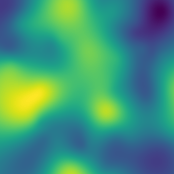
\includegraphics[interpolate=true,width=1.740000in,height=1.740000in]{random_field_regressiom-img0.png}}%
\end{pgfscope}%
\begin{pgfscope}%
\pgfsetbuttcap%
\pgfsetmiterjoin%
\definecolor{currentfill}{rgb}{1.000000,1.000000,1.000000}%
\pgfsetfillcolor{currentfill}%
\pgfsetlinewidth{0.000000pt}%
\definecolor{currentstroke}{rgb}{0.000000,0.000000,0.000000}%
\pgfsetstrokecolor{currentstroke}%
\pgfsetstrokeopacity{0.000000}%
\pgfsetdash{}{0pt}%
\pgfpathmoveto{\pgfqpoint{3.725704in}{0.096475in}}%
\pgfpathlineto{\pgfqpoint{5.462257in}{0.096475in}}%
\pgfpathlineto{\pgfqpoint{5.462257in}{1.833028in}}%
\pgfpathlineto{\pgfqpoint{3.725704in}{1.833028in}}%
\pgfpathlineto{\pgfqpoint{3.725704in}{0.096475in}}%
\pgfpathclose%
\pgfusepath{fill}%
\end{pgfscope}%
\begin{pgfscope}%
\pgfpathrectangle{\pgfqpoint{3.725704in}{0.096475in}}{\pgfqpoint{1.736553in}{1.736553in}}%
\pgfusepath{clip}%
\pgfsys@transformshift{3.725704in}{0.096475in}%
\pgftext[left,bottom]{
\includegraphics[interpolate=true,width=1.740000in,height=1.740000in]{random_field_regressiom-img1.png}}%
\end{pgfscope}%
\begin{pgfscope}%
\pgfsetbuttcap%
\pgfsetmiterjoin%
\definecolor{currentfill}{rgb}{1.000000,1.000000,1.000000}%
\pgfsetfillcolor{currentfill}%
\pgfsetlinewidth{0.000000pt}%
\definecolor{currentstroke}{rgb}{0.000000,0.000000,0.000000}%
\pgfsetstrokecolor{currentstroke}%
\pgfsetstrokeopacity{0.000000}%
\pgfsetdash{}{0pt}%
\pgfpathmoveto{\pgfqpoint{5.562257in}{0.096475in}}%
\pgfpathlineto{\pgfqpoint{5.735912in}{0.096475in}}%
\pgfpathlineto{\pgfqpoint{5.735912in}{1.833028in}}%
\pgfpathlineto{\pgfqpoint{5.562257in}{1.833028in}}%
\pgfpathlineto{\pgfqpoint{5.562257in}{0.096475in}}%
\pgfpathclose%
\pgfusepath{fill}%
\end{pgfscope}%
\begin{pgfscope}%
\pgfsys@transformshift{5.560000in}{0.109503in}%
\pgftext[left,bottom]{
\includegraphics[interpolate=true,width=0.180000in,height=1.730000in]{random_field_regressiom-img2.png}}%
\end{pgfscope}%
\begin{pgfscope}%
\pgfsetrectcap%
\pgfsetmiterjoin%
\pgfsetlinewidth{0.803000pt}%
\definecolor{currentstroke}{rgb}{0.000000,0.000000,0.000000}%
\pgfsetstrokecolor{currentstroke}%
\pgfsetdash{}{0pt}%
\pgfpathmoveto{\pgfqpoint{5.562257in}{0.096475in}}%
\pgfpathlineto{\pgfqpoint{5.649084in}{0.096475in}}%
\pgfpathlineto{\pgfqpoint{5.735912in}{0.096475in}}%
\pgfpathlineto{\pgfqpoint{5.735912in}{1.833028in}}%
\pgfpathlineto{\pgfqpoint{5.649084in}{1.833028in}}%
\pgfpathlineto{\pgfqpoint{5.562257in}{1.833028in}}%
\pgfpathlineto{\pgfqpoint{5.562257in}{0.096475in}}%
\pgfpathclose%
\pgfusepath{stroke}%
\end{pgfscope}%
\end{pgfpicture}%
\makeatother%
\endgroup%

    \caption{Gaussian random field regression: Sampled points, regression, ground truth and color bar.}
    \label{fig:random_field_regression}
\end{figure}

First we deal with the unbiasedness condition.
We can write the linear predictor as
\[
    \hat{X}_{t} = w^{T} y + c
\]
with \( w = [w_{1}, \dots, w_{n}] \) and \( y = [X_{t_{1}}, \dots, X_{t_{n}}] \).
If we require \( \hat{X_{t}} \) to be unbiased,
\[
    \mu = \E[\hat{X}_{t}] = \E[c + w^{T} y] = c + w^{T} (\mathbf{1}_{n} \mu).
\]
Here we denote by \( \mathbf{1}_{n} \) the vector of length \( n \) with all entries equal to one.
The last equality is due to the observations $y$ being distributed with mean $\mu$.
Thus the constant term must be
\[
    c = \mu - w^{T} (\mathbf{1}_{n} \mu)
\]
and the unbiased predictor is
\[
    \hat{X}_{t} = \mu + w^{T} (y- (\mathbf{1}_{n} \mu)).
\]

Before we deal with the minimization of the mean squared error, we will introduce some notation.
Let us define the vector
\[
    \begin{bmatrix}
    X_{t}\\
    \hat{X}_{M}
    \end{bmatrix},
\]
where $X_{t}$ is the random variable obtained from $X$ at a fixed $t \in T$ and $\hat{X}_{M}$ is the random vector containing measurements \( [X_{t_{1}}, \dots, X_{t_{n}}] \) at points \(M=  \{ t_{1}, \dots, t_{n} \} \subset T \).
This vector is Gaussian with mean 
\[
    \mu = \begin{bmatrix}
    \mu_{t}\\
    \mu_{M}
    \end{bmatrix}
\]
and covariance
\[
    \Sigma = \begin{bmatrix}
    \Sigma_{t,t} & \Sigma_{t, M}\\
    \Sigma_{M, t} & \Sigma_{M,M}
    \end{bmatrix},
\]
where \( \mu_{M} \coloneqq [\mu_{t_{1}}, \dots , \mu_{t_{n}}]^{T} \) 
and the covariance block matrices are given by
\begin{align*}
    \Sigma_{t,t} &= C(t,t)\\
    \Sigma_{t, M} &= [C(t,t_{i})]_{1 \leq i \leq n}\\
    \Sigma_{M, t} &= (\Sigma_{t, M})^{T}\\
    \Sigma_{M,M} &= [C(t_{i},t_{j})]_{1 \leq i,j \leq n}.
\end{align*}
Now we come to the minimization of the mean squared error.
We can reformulate it as 
\begin{align*}
    \operatorname{MSE}(\hat{X}_{t}) &= \E\left[ \left( \hat{X}_{t} - X_{t} \right)^{2} \right]\\
    &= \E\left[ (w^{T}(y-\mu)+(\mu-X_{t}))^2 \right]\\
    &= w^{T} \E[(y-\mu)(y-\mu)^{T}] w + \E[(\mu-X_{t})^2] - 2 \E[w^{T}(y-\mu)(X_{t}-\mu)]\\ 
    &= w^{T} \Sigma_{M, M} w + \Sigma_{t, t} -2 w^{T} \Sigma_{M,t}.
\end{align*}
Differentiating with respect to $w$ and setting the gradient to zero yields
\begin{align*}
    0 &= \frac{\partial}{\partial w} \left( w^{T}\Sigma_{M, M} w + \Sigma_{t, t} -2 w^{T}\Sigma_{M,t} \right) \\
    &= 2\Sigma_{M,M} w - 2 \Sigma_{M,t},
\end{align*}
which is equivalent to
\[
    \Sigma_{M,M} w = \Sigma_{M,t}.
\]
From this we derive the optimal weights \( w = \Sigma_{M,M}^{-1} \Sigma_{M,t} \).
And thus we have the Kriging predictor
\[
    \hat{X}_{t} = \mu + \Sigma_{t,M} \Sigma_{M,M}^{-1} (y-(\mathbf{1}_{n} \mu)),
\]
as well as the resulting mean squared error
\[
    \operatorname{MSE}(\hat{X}_{t}) = \Sigma_{t,t} - \Sigma_{t,M} \Sigma_{M,M}^{-1} \Sigma_{M,t}.
\]

Hence, the Kriging predictor is distributed akin to the conditional distribution of a Gaussian random vector, given the measurements, as described in \cref{lem:conditioned_gaussian_random_vector}.
That is,
\begin{equation}\label{eq:kriging_predictor}
    \hat{X}_{t} \sim \mathcal{N}\left(\mu+\Sigma_{t,M}\Sigma_{M,M}^{-1}(y-(\mathbf{1}_{n}\mu)),\,\, \Sigma_{t,t} - \Sigma_{t,M} \Sigma_{M,M}^{-1} \Sigma_{M,t} \right).
\end{equation}





% Then we know from \cref{lem:conditioned_gaussian_random_vector}, that the conditional distribution of \( X_{t^{*}} \) given \( \hat{X}_{M} \) is
% \[
%     X_{t^{*}} \mid \hat{X}_{M} \sim \mathcal{N}\left(\mu_{t^{*}} + \Sigma_{t^{*}, M} \Sigma_{M,M}^{-1} (\hat{X}_{M} - \mu_{M}),\,\, \Sigma_{t^{*},t^{*}} - \Sigma_{t^{*}, M} \Sigma_{M,M}^{-1} \Sigma_{M,t^{*}}\right).
% \]
As we have seen, Kriging provides the \textit{best linear unbiased predictor} (BLUP)\index{Kriging! BLUP property}.  
It is also an exact interpolator~\cite[p.359]{cressie1993statistics}, meaning that the predictor is exact at the measurement points.
One special property of Gaussian processes is, that the optimal predictor and optimal linear predictor are the same under squared error loss~\cite[p.110]{cressie1993statistics}.
% Without going into further detail, an alternative path to deriving Gaussian process regression is to start with a Bayesian linear regression and utilize a kernel trick as is done in~\cite[p. 156]{shahriari2015taking}.





%%%%%%%%%%%%%%%%%%%%%%%%%%%%%%%%%%%%%%%%%%%%%%%%%%%
%%%%%%%%%%%%%%%%%%%%%%%%%%%%%%%%%%%%%%%%%%%%%%%%%%%
%%% Bayesian Optimization
\section{Bayesian Optimization}~\label{sec:bayes_opt}\index{Bayesian Optimization}
% \begin{figure}[ht]
%     \centering
%     %% Creator: Matplotlib, PGF backend
%%
%% To include the figure in your LaTeX document, write
%%   \input{<filename>.pgf}
%%
%% Make sure the required packages are loaded in your preamble
%%   \usepackage{pgf}
%%
%% Also ensure that all the required font packages are loaded; for instance,
%% the lmodern package is sometimes necessary when using math font.
%%   \usepackage{lmodern}
%%
%% Figures using additional raster images can only be included by \input if
%% they are in the same directory as the main LaTeX file. For loading figures
%% from other directories you can use the `import` package
%%   \usepackage{import}
%%
%% and then include the figures with
%%   \import{<path to file>}{<filename>.pgf}
%%
%% Matplotlib used the following preamble
%%   \def\mathdefault#1{#1}
%%   \everymath=\expandafter{\the\everymath\displaystyle}
%%   \usepackage[T1]{fontenc}
%%   \usepackage{siunitx}
%%   \usepackage{amssymb}
%%   \usepackage{amsmath}
%%   \makeatletter\@ifpackageloaded{underscore}{}{\usepackage[strings]{underscore}}\makeatother
%%
\begingroup%
\makeatletter%
\begin{pgfpicture}%
\pgfpathrectangle{\pgfpointorigin}{\pgfqpoint{5.788510in}{1.929503in}}%
\pgfusepath{use as bounding box, clip}%
\begin{pgfscope}%
\pgfsetbuttcap%
\pgfsetmiterjoin%
\definecolor{currentfill}{rgb}{1.000000,1.000000,1.000000}%
\pgfsetfillcolor{currentfill}%
\pgfsetlinewidth{0.000000pt}%
\definecolor{currentstroke}{rgb}{1.000000,1.000000,1.000000}%
\pgfsetstrokecolor{currentstroke}%
\pgfsetdash{}{0pt}%
\pgfpathmoveto{\pgfqpoint{0.000000in}{0.000000in}}%
\pgfpathlineto{\pgfqpoint{5.788510in}{0.000000in}}%
\pgfpathlineto{\pgfqpoint{5.788510in}{1.929503in}}%
\pgfpathlineto{\pgfqpoint{0.000000in}{1.929503in}}%
\pgfpathlineto{\pgfqpoint{0.000000in}{0.000000in}}%
\pgfpathclose%
\pgfusepath{fill}%
\end{pgfscope}%
\begin{pgfscope}%
\pgfsetbuttcap%
\pgfsetmiterjoin%
\definecolor{currentfill}{rgb}{1.000000,1.000000,1.000000}%
\pgfsetfillcolor{currentfill}%
\pgfsetlinewidth{0.000000pt}%
\definecolor{currentstroke}{rgb}{0.000000,0.000000,0.000000}%
\pgfsetstrokecolor{currentstroke}%
\pgfsetstrokeopacity{0.000000}%
\pgfsetdash{}{0pt}%
\pgfpathmoveto{\pgfqpoint{0.000000in}{0.000000in}}%
\pgfpathlineto{\pgfqpoint{1.862837in}{0.000000in}}%
\pgfpathlineto{\pgfqpoint{1.862837in}{1.543603in}}%
\pgfpathlineto{\pgfqpoint{0.000000in}{1.543603in}}%
\pgfpathlineto{\pgfqpoint{0.000000in}{0.000000in}}%
\pgfpathclose%
\pgfusepath{fill}%
\end{pgfscope}%
\begin{pgfscope}%
\pgfpathrectangle{\pgfqpoint{0.000000in}{0.000000in}}{\pgfqpoint{1.862837in}{1.543603in}}%
\pgfusepath{clip}%
\pgfsetrectcap%
\pgfsetroundjoin%
\pgfsetlinewidth{1.505625pt}%
\definecolor{currentstroke}{rgb}{1.000000,0.745098,0.043137}%
\pgfsetstrokecolor{currentstroke}%
\pgfsetdash{}{0pt}%
\pgfpathmoveto{\pgfqpoint{0.084674in}{0.794601in}}%
\pgfpathlineto{\pgfqpoint{0.088068in}{0.800141in}}%
\pgfpathlineto{\pgfqpoint{0.091462in}{0.843520in}}%
\pgfpathlineto{\pgfqpoint{0.094856in}{0.832327in}}%
\pgfpathlineto{\pgfqpoint{0.098249in}{0.782336in}}%
\pgfpathlineto{\pgfqpoint{0.101643in}{0.838641in}}%
\pgfpathlineto{\pgfqpoint{0.108431in}{0.734274in}}%
\pgfpathlineto{\pgfqpoint{0.115218in}{0.653552in}}%
\pgfpathlineto{\pgfqpoint{0.118612in}{0.586457in}}%
\pgfpathlineto{\pgfqpoint{0.122006in}{0.573435in}}%
\pgfpathlineto{\pgfqpoint{0.128793in}{0.500916in}}%
\pgfpathlineto{\pgfqpoint{0.135581in}{0.622884in}}%
\pgfpathlineto{\pgfqpoint{0.138975in}{0.659603in}}%
\pgfpathlineto{\pgfqpoint{0.142368in}{0.636054in}}%
\pgfpathlineto{\pgfqpoint{0.145762in}{0.575947in}}%
\pgfpathlineto{\pgfqpoint{0.149156in}{0.564020in}}%
\pgfpathlineto{\pgfqpoint{0.152550in}{0.488547in}}%
\pgfpathlineto{\pgfqpoint{0.155943in}{0.479965in}}%
\pgfpathlineto{\pgfqpoint{0.159337in}{0.517646in}}%
\pgfpathlineto{\pgfqpoint{0.162731in}{0.513031in}}%
\pgfpathlineto{\pgfqpoint{0.166125in}{0.621216in}}%
\pgfpathlineto{\pgfqpoint{0.169518in}{0.580526in}}%
\pgfpathlineto{\pgfqpoint{0.172912in}{0.501333in}}%
\pgfpathlineto{\pgfqpoint{0.176306in}{0.523073in}}%
\pgfpathlineto{\pgfqpoint{0.179700in}{0.497368in}}%
\pgfpathlineto{\pgfqpoint{0.183094in}{0.423849in}}%
\pgfpathlineto{\pgfqpoint{0.186487in}{0.514603in}}%
\pgfpathlineto{\pgfqpoint{0.189881in}{0.421164in}}%
\pgfpathlineto{\pgfqpoint{0.193275in}{0.492301in}}%
\pgfpathlineto{\pgfqpoint{0.196669in}{0.499656in}}%
\pgfpathlineto{\pgfqpoint{0.200062in}{0.452382in}}%
\pgfpathlineto{\pgfqpoint{0.203456in}{0.474955in}}%
\pgfpathlineto{\pgfqpoint{0.213637in}{0.594596in}}%
\pgfpathlineto{\pgfqpoint{0.217031in}{0.610689in}}%
\pgfpathlineto{\pgfqpoint{0.223819in}{0.510253in}}%
\pgfpathlineto{\pgfqpoint{0.230606in}{0.738383in}}%
\pgfpathlineto{\pgfqpoint{0.234000in}{0.734122in}}%
\pgfpathlineto{\pgfqpoint{0.237394in}{0.879214in}}%
\pgfpathlineto{\pgfqpoint{0.240788in}{0.875446in}}%
\pgfpathlineto{\pgfqpoint{0.244181in}{0.842498in}}%
\pgfpathlineto{\pgfqpoint{0.247575in}{0.780322in}}%
\pgfpathlineto{\pgfqpoint{0.250969in}{0.670981in}}%
\pgfpathlineto{\pgfqpoint{0.254363in}{0.670008in}}%
\pgfpathlineto{\pgfqpoint{0.257756in}{0.584142in}}%
\pgfpathlineto{\pgfqpoint{0.261150in}{0.562389in}}%
\pgfpathlineto{\pgfqpoint{0.264544in}{0.549206in}}%
\pgfpathlineto{\pgfqpoint{0.267938in}{0.526757in}}%
\pgfpathlineto{\pgfqpoint{0.271331in}{0.491184in}}%
\pgfpathlineto{\pgfqpoint{0.274725in}{0.522678in}}%
\pgfpathlineto{\pgfqpoint{0.278119in}{0.447986in}}%
\pgfpathlineto{\pgfqpoint{0.281513in}{0.470525in}}%
\pgfpathlineto{\pgfqpoint{0.284906in}{0.483481in}}%
\pgfpathlineto{\pgfqpoint{0.288300in}{0.566694in}}%
\pgfpathlineto{\pgfqpoint{0.291694in}{0.575801in}}%
\pgfpathlineto{\pgfqpoint{0.295088in}{0.630565in}}%
\pgfpathlineto{\pgfqpoint{0.298481in}{0.659792in}}%
\pgfpathlineto{\pgfqpoint{0.301875in}{0.718138in}}%
\pgfpathlineto{\pgfqpoint{0.305269in}{0.805648in}}%
\pgfpathlineto{\pgfqpoint{0.308663in}{0.780472in}}%
\pgfpathlineto{\pgfqpoint{0.312057in}{0.770071in}}%
\pgfpathlineto{\pgfqpoint{0.315450in}{0.748643in}}%
\pgfpathlineto{\pgfqpoint{0.318844in}{0.829520in}}%
\pgfpathlineto{\pgfqpoint{0.322238in}{0.877246in}}%
\pgfpathlineto{\pgfqpoint{0.325632in}{0.957295in}}%
\pgfpathlineto{\pgfqpoint{0.329025in}{0.882394in}}%
\pgfpathlineto{\pgfqpoint{0.332419in}{0.908486in}}%
\pgfpathlineto{\pgfqpoint{0.335813in}{0.880731in}}%
\pgfpathlineto{\pgfqpoint{0.339207in}{0.893594in}}%
\pgfpathlineto{\pgfqpoint{0.342600in}{0.925660in}}%
\pgfpathlineto{\pgfqpoint{0.345994in}{0.890903in}}%
\pgfpathlineto{\pgfqpoint{0.352782in}{0.872103in}}%
\pgfpathlineto{\pgfqpoint{0.356175in}{1.041897in}}%
\pgfpathlineto{\pgfqpoint{0.359569in}{1.073514in}}%
\pgfpathlineto{\pgfqpoint{0.362963in}{1.077549in}}%
\pgfpathlineto{\pgfqpoint{0.366357in}{1.060886in}}%
\pgfpathlineto{\pgfqpoint{0.369751in}{0.948955in}}%
\pgfpathlineto{\pgfqpoint{0.373144in}{0.981017in}}%
\pgfpathlineto{\pgfqpoint{0.376538in}{0.981860in}}%
\pgfpathlineto{\pgfqpoint{0.379932in}{0.938528in}}%
\pgfpathlineto{\pgfqpoint{0.383326in}{0.919916in}}%
\pgfpathlineto{\pgfqpoint{0.386719in}{0.797727in}}%
\pgfpathlineto{\pgfqpoint{0.393507in}{0.703608in}}%
\pgfpathlineto{\pgfqpoint{0.396901in}{0.829789in}}%
\pgfpathlineto{\pgfqpoint{0.400294in}{0.869064in}}%
\pgfpathlineto{\pgfqpoint{0.403688in}{0.837591in}}%
\pgfpathlineto{\pgfqpoint{0.407082in}{0.856003in}}%
\pgfpathlineto{\pgfqpoint{0.410476in}{0.742361in}}%
\pgfpathlineto{\pgfqpoint{0.413869in}{0.789394in}}%
\pgfpathlineto{\pgfqpoint{0.424051in}{0.626486in}}%
\pgfpathlineto{\pgfqpoint{0.434232in}{0.819015in}}%
\pgfpathlineto{\pgfqpoint{0.437626in}{0.719856in}}%
\pgfpathlineto{\pgfqpoint{0.441020in}{0.815905in}}%
\pgfpathlineto{\pgfqpoint{0.444413in}{0.823017in}}%
\pgfpathlineto{\pgfqpoint{0.447807in}{0.900181in}}%
\pgfpathlineto{\pgfqpoint{0.451201in}{0.822757in}}%
\pgfpathlineto{\pgfqpoint{0.454595in}{0.907094in}}%
\pgfpathlineto{\pgfqpoint{0.457988in}{0.870803in}}%
\pgfpathlineto{\pgfqpoint{0.461382in}{0.922417in}}%
\pgfpathlineto{\pgfqpoint{0.464776in}{0.915768in}}%
\pgfpathlineto{\pgfqpoint{0.468170in}{0.941156in}}%
\pgfpathlineto{\pgfqpoint{0.471563in}{0.890489in}}%
\pgfpathlineto{\pgfqpoint{0.474957in}{0.938581in}}%
\pgfpathlineto{\pgfqpoint{0.478351in}{0.948544in}}%
\pgfpathlineto{\pgfqpoint{0.481745in}{0.941782in}}%
\pgfpathlineto{\pgfqpoint{0.485138in}{0.940491in}}%
\pgfpathlineto{\pgfqpoint{0.488532in}{1.041011in}}%
\pgfpathlineto{\pgfqpoint{0.491926in}{0.937540in}}%
\pgfpathlineto{\pgfqpoint{0.495320in}{0.955196in}}%
\pgfpathlineto{\pgfqpoint{0.498714in}{0.986336in}}%
\pgfpathlineto{\pgfqpoint{0.502107in}{0.990939in}}%
\pgfpathlineto{\pgfqpoint{0.508895in}{0.928581in}}%
\pgfpathlineto{\pgfqpoint{0.512289in}{1.044449in}}%
\pgfpathlineto{\pgfqpoint{0.519076in}{0.909995in}}%
\pgfpathlineto{\pgfqpoint{0.522470in}{0.914298in}}%
\pgfpathlineto{\pgfqpoint{0.529257in}{0.881311in}}%
\pgfpathlineto{\pgfqpoint{0.532651in}{0.772330in}}%
\pgfpathlineto{\pgfqpoint{0.536045in}{0.745058in}}%
\pgfpathlineto{\pgfqpoint{0.539439in}{0.731497in}}%
\pgfpathlineto{\pgfqpoint{0.542832in}{0.679800in}}%
\pgfpathlineto{\pgfqpoint{0.549620in}{0.538851in}}%
\pgfpathlineto{\pgfqpoint{0.553014in}{0.417893in}}%
\pgfpathlineto{\pgfqpoint{0.559801in}{0.488948in}}%
\pgfpathlineto{\pgfqpoint{0.563195in}{0.481162in}}%
\pgfpathlineto{\pgfqpoint{0.566589in}{0.417272in}}%
\pgfpathlineto{\pgfqpoint{0.569983in}{0.441192in}}%
\pgfpathlineto{\pgfqpoint{0.573376in}{0.406436in}}%
\pgfpathlineto{\pgfqpoint{0.576770in}{0.459620in}}%
\pgfpathlineto{\pgfqpoint{0.580164in}{0.441007in}}%
\pgfpathlineto{\pgfqpoint{0.583558in}{0.268714in}}%
\pgfpathlineto{\pgfqpoint{0.586951in}{0.231825in}}%
\pgfpathlineto{\pgfqpoint{0.590345in}{0.218376in}}%
\pgfpathlineto{\pgfqpoint{0.593739in}{0.261754in}}%
\pgfpathlineto{\pgfqpoint{0.597133in}{0.215782in}}%
\pgfpathlineto{\pgfqpoint{0.603920in}{0.280865in}}%
\pgfpathlineto{\pgfqpoint{0.607314in}{0.268995in}}%
\pgfpathlineto{\pgfqpoint{0.610708in}{0.291653in}}%
\pgfpathlineto{\pgfqpoint{0.614101in}{0.245422in}}%
\pgfpathlineto{\pgfqpoint{0.617495in}{0.376202in}}%
\pgfpathlineto{\pgfqpoint{0.620889in}{0.347949in}}%
\pgfpathlineto{\pgfqpoint{0.624283in}{0.345189in}}%
\pgfpathlineto{\pgfqpoint{0.631070in}{0.531842in}}%
\pgfpathlineto{\pgfqpoint{0.634464in}{0.606281in}}%
\pgfpathlineto{\pgfqpoint{0.637858in}{0.608076in}}%
\pgfpathlineto{\pgfqpoint{0.644645in}{0.537153in}}%
\pgfpathlineto{\pgfqpoint{0.648039in}{0.473644in}}%
\pgfpathlineto{\pgfqpoint{0.651433in}{0.378194in}}%
\pgfpathlineto{\pgfqpoint{0.654827in}{0.385370in}}%
\pgfpathlineto{\pgfqpoint{0.658220in}{0.399761in}}%
\pgfpathlineto{\pgfqpoint{0.661614in}{0.499167in}}%
\pgfpathlineto{\pgfqpoint{0.665008in}{0.557760in}}%
\pgfpathlineto{\pgfqpoint{0.668402in}{0.510117in}}%
\pgfpathlineto{\pgfqpoint{0.671795in}{0.437618in}}%
\pgfpathlineto{\pgfqpoint{0.675189in}{0.394997in}}%
\pgfpathlineto{\pgfqpoint{0.678583in}{0.379174in}}%
\pgfpathlineto{\pgfqpoint{0.681977in}{0.408936in}}%
\pgfpathlineto{\pgfqpoint{0.685370in}{0.339646in}}%
\pgfpathlineto{\pgfqpoint{0.692158in}{0.433938in}}%
\pgfpathlineto{\pgfqpoint{0.695552in}{0.440122in}}%
\pgfpathlineto{\pgfqpoint{0.698946in}{0.457137in}}%
\pgfpathlineto{\pgfqpoint{0.702339in}{0.392158in}}%
\pgfpathlineto{\pgfqpoint{0.705733in}{0.377136in}}%
\pgfpathlineto{\pgfqpoint{0.712521in}{0.261312in}}%
\pgfpathlineto{\pgfqpoint{0.715914in}{0.303187in}}%
\pgfpathlineto{\pgfqpoint{0.719308in}{0.296121in}}%
\pgfpathlineto{\pgfqpoint{0.722702in}{0.417970in}}%
\pgfpathlineto{\pgfqpoint{0.726096in}{0.410152in}}%
\pgfpathlineto{\pgfqpoint{0.729489in}{0.512061in}}%
\pgfpathlineto{\pgfqpoint{0.732883in}{0.499741in}}%
\pgfpathlineto{\pgfqpoint{0.739671in}{0.274851in}}%
\pgfpathlineto{\pgfqpoint{0.743064in}{0.211694in}}%
\pgfpathlineto{\pgfqpoint{0.746458in}{0.201734in}}%
\pgfpathlineto{\pgfqpoint{0.749852in}{0.182799in}}%
\pgfpathlineto{\pgfqpoint{0.753246in}{0.146030in}}%
\pgfpathlineto{\pgfqpoint{0.756640in}{0.144529in}}%
\pgfpathlineto{\pgfqpoint{0.760033in}{0.112254in}}%
\pgfpathlineto{\pgfqpoint{0.766821in}{0.181552in}}%
\pgfpathlineto{\pgfqpoint{0.770215in}{0.293583in}}%
\pgfpathlineto{\pgfqpoint{0.773608in}{0.291707in}}%
\pgfpathlineto{\pgfqpoint{0.777002in}{0.351681in}}%
\pgfpathlineto{\pgfqpoint{0.780396in}{0.384255in}}%
\pgfpathlineto{\pgfqpoint{0.783790in}{0.404062in}}%
\pgfpathlineto{\pgfqpoint{0.787183in}{0.403956in}}%
\pgfpathlineto{\pgfqpoint{0.790577in}{0.470485in}}%
\pgfpathlineto{\pgfqpoint{0.793971in}{0.422794in}}%
\pgfpathlineto{\pgfqpoint{0.797365in}{0.412214in}}%
\pgfpathlineto{\pgfqpoint{0.804152in}{0.498025in}}%
\pgfpathlineto{\pgfqpoint{0.807546in}{0.416758in}}%
\pgfpathlineto{\pgfqpoint{0.810940in}{0.386592in}}%
\pgfpathlineto{\pgfqpoint{0.814334in}{0.400034in}}%
\pgfpathlineto{\pgfqpoint{0.817727in}{0.534187in}}%
\pgfpathlineto{\pgfqpoint{0.821121in}{0.499206in}}%
\pgfpathlineto{\pgfqpoint{0.827909in}{0.570838in}}%
\pgfpathlineto{\pgfqpoint{0.838090in}{0.280138in}}%
\pgfpathlineto{\pgfqpoint{0.841484in}{0.345131in}}%
\pgfpathlineto{\pgfqpoint{0.844877in}{0.338009in}}%
\pgfpathlineto{\pgfqpoint{0.848271in}{0.428982in}}%
\pgfpathlineto{\pgfqpoint{0.851665in}{0.418503in}}%
\pgfpathlineto{\pgfqpoint{0.855059in}{0.441672in}}%
\pgfpathlineto{\pgfqpoint{0.858452in}{0.401483in}}%
\pgfpathlineto{\pgfqpoint{0.861846in}{0.398558in}}%
\pgfpathlineto{\pgfqpoint{0.865240in}{0.456837in}}%
\pgfpathlineto{\pgfqpoint{0.868634in}{0.489040in}}%
\pgfpathlineto{\pgfqpoint{0.872027in}{0.535954in}}%
\pgfpathlineto{\pgfqpoint{0.875421in}{0.534264in}}%
\pgfpathlineto{\pgfqpoint{0.878815in}{0.504860in}}%
\pgfpathlineto{\pgfqpoint{0.882209in}{0.377862in}}%
\pgfpathlineto{\pgfqpoint{0.888996in}{0.397333in}}%
\pgfpathlineto{\pgfqpoint{0.892390in}{0.437727in}}%
\pgfpathlineto{\pgfqpoint{0.895784in}{0.429798in}}%
\pgfpathlineto{\pgfqpoint{0.899178in}{0.429138in}}%
\pgfpathlineto{\pgfqpoint{0.902571in}{0.402263in}}%
\pgfpathlineto{\pgfqpoint{0.905965in}{0.451877in}}%
\pgfpathlineto{\pgfqpoint{0.909359in}{0.483298in}}%
\pgfpathlineto{\pgfqpoint{0.912753in}{0.463268in}}%
\pgfpathlineto{\pgfqpoint{0.916146in}{0.497053in}}%
\pgfpathlineto{\pgfqpoint{0.919540in}{0.483771in}}%
\pgfpathlineto{\pgfqpoint{0.926328in}{0.531193in}}%
\pgfpathlineto{\pgfqpoint{0.929721in}{0.639191in}}%
\pgfpathlineto{\pgfqpoint{0.933115in}{0.654669in}}%
\pgfpathlineto{\pgfqpoint{0.936509in}{0.762931in}}%
\pgfpathlineto{\pgfqpoint{0.939903in}{0.806802in}}%
\pgfpathlineto{\pgfqpoint{0.943297in}{0.923650in}}%
\pgfpathlineto{\pgfqpoint{0.946690in}{0.832904in}}%
\pgfpathlineto{\pgfqpoint{0.950084in}{0.809933in}}%
\pgfpathlineto{\pgfqpoint{0.953478in}{0.755027in}}%
\pgfpathlineto{\pgfqpoint{0.956872in}{0.743059in}}%
\pgfpathlineto{\pgfqpoint{0.960265in}{0.813688in}}%
\pgfpathlineto{\pgfqpoint{0.963659in}{0.856109in}}%
\pgfpathlineto{\pgfqpoint{0.967053in}{0.808293in}}%
\pgfpathlineto{\pgfqpoint{0.970447in}{0.731482in}}%
\pgfpathlineto{\pgfqpoint{0.973840in}{0.740658in}}%
\pgfpathlineto{\pgfqpoint{0.977234in}{0.826618in}}%
\pgfpathlineto{\pgfqpoint{0.980628in}{0.811920in}}%
\pgfpathlineto{\pgfqpoint{0.984022in}{0.815050in}}%
\pgfpathlineto{\pgfqpoint{0.987415in}{0.918094in}}%
\pgfpathlineto{\pgfqpoint{0.997597in}{0.763263in}}%
\pgfpathlineto{\pgfqpoint{1.000990in}{0.749362in}}%
\pgfpathlineto{\pgfqpoint{1.004384in}{0.849175in}}%
\pgfpathlineto{\pgfqpoint{1.007778in}{0.865090in}}%
\pgfpathlineto{\pgfqpoint{1.011172in}{0.896889in}}%
\pgfpathlineto{\pgfqpoint{1.014566in}{0.894491in}}%
\pgfpathlineto{\pgfqpoint{1.017959in}{0.944619in}}%
\pgfpathlineto{\pgfqpoint{1.021353in}{0.961588in}}%
\pgfpathlineto{\pgfqpoint{1.024747in}{0.995147in}}%
\pgfpathlineto{\pgfqpoint{1.028141in}{1.097370in}}%
\pgfpathlineto{\pgfqpoint{1.034928in}{0.980240in}}%
\pgfpathlineto{\pgfqpoint{1.038322in}{0.999775in}}%
\pgfpathlineto{\pgfqpoint{1.041716in}{1.086775in}}%
\pgfpathlineto{\pgfqpoint{1.045109in}{1.127242in}}%
\pgfpathlineto{\pgfqpoint{1.048503in}{1.123273in}}%
\pgfpathlineto{\pgfqpoint{1.051897in}{1.041224in}}%
\pgfpathlineto{\pgfqpoint{1.055291in}{1.060619in}}%
\pgfpathlineto{\pgfqpoint{1.058684in}{1.052431in}}%
\pgfpathlineto{\pgfqpoint{1.062078in}{1.056697in}}%
\pgfpathlineto{\pgfqpoint{1.065472in}{0.988305in}}%
\pgfpathlineto{\pgfqpoint{1.068866in}{1.012744in}}%
\pgfpathlineto{\pgfqpoint{1.072260in}{0.949479in}}%
\pgfpathlineto{\pgfqpoint{1.075653in}{0.986408in}}%
\pgfpathlineto{\pgfqpoint{1.079047in}{0.995747in}}%
\pgfpathlineto{\pgfqpoint{1.082441in}{0.945127in}}%
\pgfpathlineto{\pgfqpoint{1.085835in}{0.921718in}}%
\pgfpathlineto{\pgfqpoint{1.089228in}{0.925037in}}%
\pgfpathlineto{\pgfqpoint{1.092622in}{0.966926in}}%
\pgfpathlineto{\pgfqpoint{1.096016in}{0.966601in}}%
\pgfpathlineto{\pgfqpoint{1.102803in}{0.912672in}}%
\pgfpathlineto{\pgfqpoint{1.106197in}{0.923186in}}%
\pgfpathlineto{\pgfqpoint{1.109591in}{0.967564in}}%
\pgfpathlineto{\pgfqpoint{1.112985in}{0.912731in}}%
\pgfpathlineto{\pgfqpoint{1.116378in}{0.830751in}}%
\pgfpathlineto{\pgfqpoint{1.119772in}{0.894348in}}%
\pgfpathlineto{\pgfqpoint{1.123166in}{0.850159in}}%
\pgfpathlineto{\pgfqpoint{1.126560in}{0.882282in}}%
\pgfpathlineto{\pgfqpoint{1.129953in}{0.943172in}}%
\pgfpathlineto{\pgfqpoint{1.140135in}{1.049953in}}%
\pgfpathlineto{\pgfqpoint{1.143529in}{1.067706in}}%
\pgfpathlineto{\pgfqpoint{1.146922in}{1.146946in}}%
\pgfpathlineto{\pgfqpoint{1.150316in}{1.155618in}}%
\pgfpathlineto{\pgfqpoint{1.153710in}{1.204583in}}%
\pgfpathlineto{\pgfqpoint{1.157104in}{1.107286in}}%
\pgfpathlineto{\pgfqpoint{1.163891in}{1.144038in}}%
\pgfpathlineto{\pgfqpoint{1.167285in}{1.182218in}}%
\pgfpathlineto{\pgfqpoint{1.174072in}{1.139473in}}%
\pgfpathlineto{\pgfqpoint{1.177466in}{1.244435in}}%
\pgfpathlineto{\pgfqpoint{1.180860in}{1.273987in}}%
\pgfpathlineto{\pgfqpoint{1.184254in}{1.265614in}}%
\pgfpathlineto{\pgfqpoint{1.187647in}{1.269794in}}%
\pgfpathlineto{\pgfqpoint{1.191041in}{1.212851in}}%
\pgfpathlineto{\pgfqpoint{1.194435in}{1.200355in}}%
\pgfpathlineto{\pgfqpoint{1.197829in}{1.138304in}}%
\pgfpathlineto{\pgfqpoint{1.201223in}{1.020700in}}%
\pgfpathlineto{\pgfqpoint{1.204616in}{1.036248in}}%
\pgfpathlineto{\pgfqpoint{1.208010in}{1.060197in}}%
\pgfpathlineto{\pgfqpoint{1.211404in}{1.001804in}}%
\pgfpathlineto{\pgfqpoint{1.214798in}{1.010230in}}%
\pgfpathlineto{\pgfqpoint{1.218191in}{0.953972in}}%
\pgfpathlineto{\pgfqpoint{1.221585in}{0.936093in}}%
\pgfpathlineto{\pgfqpoint{1.224979in}{0.927516in}}%
\pgfpathlineto{\pgfqpoint{1.228373in}{0.879520in}}%
\pgfpathlineto{\pgfqpoint{1.231766in}{0.888602in}}%
\pgfpathlineto{\pgfqpoint{1.235160in}{0.861786in}}%
\pgfpathlineto{\pgfqpoint{1.238554in}{0.765742in}}%
\pgfpathlineto{\pgfqpoint{1.241948in}{0.845269in}}%
\pgfpathlineto{\pgfqpoint{1.245341in}{0.891173in}}%
\pgfpathlineto{\pgfqpoint{1.252129in}{0.919360in}}%
\pgfpathlineto{\pgfqpoint{1.255523in}{1.088651in}}%
\pgfpathlineto{\pgfqpoint{1.258916in}{1.060596in}}%
\pgfpathlineto{\pgfqpoint{1.262310in}{1.004946in}}%
\pgfpathlineto{\pgfqpoint{1.265704in}{1.153778in}}%
\pgfpathlineto{\pgfqpoint{1.269098in}{1.156403in}}%
\pgfpathlineto{\pgfqpoint{1.272492in}{1.160727in}}%
\pgfpathlineto{\pgfqpoint{1.275885in}{1.144723in}}%
\pgfpathlineto{\pgfqpoint{1.279279in}{1.216861in}}%
\pgfpathlineto{\pgfqpoint{1.282673in}{1.117989in}}%
\pgfpathlineto{\pgfqpoint{1.286067in}{1.209630in}}%
\pgfpathlineto{\pgfqpoint{1.289460in}{1.223398in}}%
\pgfpathlineto{\pgfqpoint{1.292854in}{1.309128in}}%
\pgfpathlineto{\pgfqpoint{1.296248in}{1.121963in}}%
\pgfpathlineto{\pgfqpoint{1.303035in}{1.115855in}}%
\pgfpathlineto{\pgfqpoint{1.306429in}{1.036648in}}%
\pgfpathlineto{\pgfqpoint{1.309823in}{1.032034in}}%
\pgfpathlineto{\pgfqpoint{1.313217in}{1.071907in}}%
\pgfpathlineto{\pgfqpoint{1.320004in}{1.260962in}}%
\pgfpathlineto{\pgfqpoint{1.323398in}{1.167687in}}%
\pgfpathlineto{\pgfqpoint{1.326792in}{1.213986in}}%
\pgfpathlineto{\pgfqpoint{1.330186in}{1.310606in}}%
\pgfpathlineto{\pgfqpoint{1.333579in}{1.335309in}}%
\pgfpathlineto{\pgfqpoint{1.336973in}{1.304312in}}%
\pgfpathlineto{\pgfqpoint{1.340367in}{1.345923in}}%
\pgfpathlineto{\pgfqpoint{1.343761in}{1.266182in}}%
\pgfpathlineto{\pgfqpoint{1.347154in}{1.253627in}}%
\pgfpathlineto{\pgfqpoint{1.350548in}{1.279891in}}%
\pgfpathlineto{\pgfqpoint{1.353942in}{1.267971in}}%
\pgfpathlineto{\pgfqpoint{1.357336in}{1.251258in}}%
\pgfpathlineto{\pgfqpoint{1.360729in}{1.110731in}}%
\pgfpathlineto{\pgfqpoint{1.364123in}{1.111223in}}%
\pgfpathlineto{\pgfqpoint{1.367517in}{1.012808in}}%
\pgfpathlineto{\pgfqpoint{1.370911in}{0.946784in}}%
\pgfpathlineto{\pgfqpoint{1.374304in}{1.015236in}}%
\pgfpathlineto{\pgfqpoint{1.377698in}{0.986713in}}%
\pgfpathlineto{\pgfqpoint{1.381092in}{0.978660in}}%
\pgfpathlineto{\pgfqpoint{1.384486in}{0.944358in}}%
\pgfpathlineto{\pgfqpoint{1.387879in}{0.829487in}}%
\pgfpathlineto{\pgfqpoint{1.391273in}{0.779146in}}%
\pgfpathlineto{\pgfqpoint{1.394667in}{0.556153in}}%
\pgfpathlineto{\pgfqpoint{1.398061in}{0.679054in}}%
\pgfpathlineto{\pgfqpoint{1.401455in}{0.612905in}}%
\pgfpathlineto{\pgfqpoint{1.404848in}{0.518401in}}%
\pgfpathlineto{\pgfqpoint{1.408242in}{0.500289in}}%
\pgfpathlineto{\pgfqpoint{1.411636in}{0.552903in}}%
\pgfpathlineto{\pgfqpoint{1.415030in}{0.655185in}}%
\pgfpathlineto{\pgfqpoint{1.418423in}{0.633972in}}%
\pgfpathlineto{\pgfqpoint{1.421817in}{0.655238in}}%
\pgfpathlineto{\pgfqpoint{1.425211in}{0.587674in}}%
\pgfpathlineto{\pgfqpoint{1.428605in}{0.567330in}}%
\pgfpathlineto{\pgfqpoint{1.431998in}{0.454111in}}%
\pgfpathlineto{\pgfqpoint{1.435392in}{0.553691in}}%
\pgfpathlineto{\pgfqpoint{1.442180in}{0.602285in}}%
\pgfpathlineto{\pgfqpoint{1.445573in}{0.571148in}}%
\pgfpathlineto{\pgfqpoint{1.448967in}{0.557171in}}%
\pgfpathlineto{\pgfqpoint{1.452361in}{0.605764in}}%
\pgfpathlineto{\pgfqpoint{1.455755in}{0.627018in}}%
\pgfpathlineto{\pgfqpoint{1.459149in}{0.480526in}}%
\pgfpathlineto{\pgfqpoint{1.462542in}{0.564506in}}%
\pgfpathlineto{\pgfqpoint{1.465936in}{0.506406in}}%
\pgfpathlineto{\pgfqpoint{1.469330in}{0.427466in}}%
\pgfpathlineto{\pgfqpoint{1.472724in}{0.460340in}}%
\pgfpathlineto{\pgfqpoint{1.476117in}{0.521534in}}%
\pgfpathlineto{\pgfqpoint{1.479511in}{0.476555in}}%
\pgfpathlineto{\pgfqpoint{1.482905in}{0.449489in}}%
\pgfpathlineto{\pgfqpoint{1.486299in}{0.412670in}}%
\pgfpathlineto{\pgfqpoint{1.489692in}{0.429609in}}%
\pgfpathlineto{\pgfqpoint{1.493086in}{0.429217in}}%
\pgfpathlineto{\pgfqpoint{1.496480in}{0.459698in}}%
\pgfpathlineto{\pgfqpoint{1.499874in}{0.462473in}}%
\pgfpathlineto{\pgfqpoint{1.503267in}{0.494901in}}%
\pgfpathlineto{\pgfqpoint{1.506661in}{0.562246in}}%
\pgfpathlineto{\pgfqpoint{1.510055in}{0.503014in}}%
\pgfpathlineto{\pgfqpoint{1.513449in}{0.474966in}}%
\pgfpathlineto{\pgfqpoint{1.516842in}{0.543716in}}%
\pgfpathlineto{\pgfqpoint{1.520236in}{0.540902in}}%
\pgfpathlineto{\pgfqpoint{1.527024in}{0.685182in}}%
\pgfpathlineto{\pgfqpoint{1.530418in}{0.622268in}}%
\pgfpathlineto{\pgfqpoint{1.533811in}{0.685064in}}%
\pgfpathlineto{\pgfqpoint{1.537205in}{0.674797in}}%
\pgfpathlineto{\pgfqpoint{1.540599in}{0.702869in}}%
\pgfpathlineto{\pgfqpoint{1.543993in}{0.719372in}}%
\pgfpathlineto{\pgfqpoint{1.547386in}{0.658541in}}%
\pgfpathlineto{\pgfqpoint{1.550780in}{0.650738in}}%
\pgfpathlineto{\pgfqpoint{1.554174in}{0.627787in}}%
\pgfpathlineto{\pgfqpoint{1.557568in}{0.628131in}}%
\pgfpathlineto{\pgfqpoint{1.560961in}{0.519515in}}%
\pgfpathlineto{\pgfqpoint{1.564355in}{0.579011in}}%
\pgfpathlineto{\pgfqpoint{1.567749in}{0.560863in}}%
\pgfpathlineto{\pgfqpoint{1.571143in}{0.490441in}}%
\pgfpathlineto{\pgfqpoint{1.574536in}{0.492444in}}%
\pgfpathlineto{\pgfqpoint{1.577930in}{0.447521in}}%
\pgfpathlineto{\pgfqpoint{1.581324in}{0.464513in}}%
\pgfpathlineto{\pgfqpoint{1.584718in}{0.354877in}}%
\pgfpathlineto{\pgfqpoint{1.588112in}{0.337778in}}%
\pgfpathlineto{\pgfqpoint{1.591505in}{0.301495in}}%
\pgfpathlineto{\pgfqpoint{1.594899in}{0.354742in}}%
\pgfpathlineto{\pgfqpoint{1.598293in}{0.324853in}}%
\pgfpathlineto{\pgfqpoint{1.601687in}{0.330543in}}%
\pgfpathlineto{\pgfqpoint{1.605080in}{0.406942in}}%
\pgfpathlineto{\pgfqpoint{1.608474in}{0.435610in}}%
\pgfpathlineto{\pgfqpoint{1.611868in}{0.259522in}}%
\pgfpathlineto{\pgfqpoint{1.615262in}{0.281960in}}%
\pgfpathlineto{\pgfqpoint{1.618655in}{0.357054in}}%
\pgfpathlineto{\pgfqpoint{1.625443in}{0.320921in}}%
\pgfpathlineto{\pgfqpoint{1.628837in}{0.434913in}}%
\pgfpathlineto{\pgfqpoint{1.632230in}{0.400834in}}%
\pgfpathlineto{\pgfqpoint{1.635624in}{0.445401in}}%
\pgfpathlineto{\pgfqpoint{1.639018in}{0.439076in}}%
\pgfpathlineto{\pgfqpoint{1.642412in}{0.334081in}}%
\pgfpathlineto{\pgfqpoint{1.645806in}{0.316220in}}%
\pgfpathlineto{\pgfqpoint{1.649199in}{0.358047in}}%
\pgfpathlineto{\pgfqpoint{1.652593in}{0.370734in}}%
\pgfpathlineto{\pgfqpoint{1.655987in}{0.405639in}}%
\pgfpathlineto{\pgfqpoint{1.659381in}{0.465890in}}%
\pgfpathlineto{\pgfqpoint{1.662774in}{0.437687in}}%
\pgfpathlineto{\pgfqpoint{1.669562in}{0.338376in}}%
\pgfpathlineto{\pgfqpoint{1.672956in}{0.321271in}}%
\pgfpathlineto{\pgfqpoint{1.676349in}{0.379725in}}%
\pgfpathlineto{\pgfqpoint{1.679743in}{0.340935in}}%
\pgfpathlineto{\pgfqpoint{1.683137in}{0.214241in}}%
\pgfpathlineto{\pgfqpoint{1.686531in}{0.192851in}}%
\pgfpathlineto{\pgfqpoint{1.693318in}{0.310462in}}%
\pgfpathlineto{\pgfqpoint{1.696712in}{0.405195in}}%
\pgfpathlineto{\pgfqpoint{1.700106in}{0.387869in}}%
\pgfpathlineto{\pgfqpoint{1.703499in}{0.323909in}}%
\pgfpathlineto{\pgfqpoint{1.706893in}{0.301187in}}%
\pgfpathlineto{\pgfqpoint{1.710287in}{0.290037in}}%
\pgfpathlineto{\pgfqpoint{1.713681in}{0.187063in}}%
\pgfpathlineto{\pgfqpoint{1.717075in}{0.177587in}}%
\pgfpathlineto{\pgfqpoint{1.720468in}{0.162924in}}%
\pgfpathlineto{\pgfqpoint{1.723862in}{0.094133in}}%
\pgfpathlineto{\pgfqpoint{1.727256in}{0.088827in}}%
\pgfpathlineto{\pgfqpoint{1.730650in}{0.135385in}}%
\pgfpathlineto{\pgfqpoint{1.734043in}{0.163753in}}%
\pgfpathlineto{\pgfqpoint{1.737437in}{0.137909in}}%
\pgfpathlineto{\pgfqpoint{1.740831in}{0.209772in}}%
\pgfpathlineto{\pgfqpoint{1.744225in}{0.177943in}}%
\pgfpathlineto{\pgfqpoint{1.747618in}{0.299179in}}%
\pgfpathlineto{\pgfqpoint{1.751012in}{0.281498in}}%
\pgfpathlineto{\pgfqpoint{1.754406in}{0.336095in}}%
\pgfpathlineto{\pgfqpoint{1.757800in}{0.325648in}}%
\pgfpathlineto{\pgfqpoint{1.761193in}{0.311020in}}%
\pgfpathlineto{\pgfqpoint{1.764587in}{0.355586in}}%
\pgfpathlineto{\pgfqpoint{1.767981in}{0.510371in}}%
\pgfpathlineto{\pgfqpoint{1.771375in}{0.461857in}}%
\pgfpathlineto{\pgfqpoint{1.774769in}{0.482427in}}%
\pgfpathlineto{\pgfqpoint{1.778162in}{0.516227in}}%
\pgfpathlineto{\pgfqpoint{1.778162in}{0.516227in}}%
\pgfusepath{stroke}%
\end{pgfscope}%
\begin{pgfscope}%
\pgfpathrectangle{\pgfqpoint{0.000000in}{0.000000in}}{\pgfqpoint{1.862837in}{1.543603in}}%
\pgfusepath{clip}%
\pgfsetrectcap%
\pgfsetroundjoin%
\pgfsetlinewidth{1.505625pt}%
\definecolor{currentstroke}{rgb}{0.984314,0.337255,0.027451}%
\pgfsetstrokecolor{currentstroke}%
\pgfsetdash{}{0pt}%
\pgfpathmoveto{\pgfqpoint{0.084674in}{0.895836in}}%
\pgfpathlineto{\pgfqpoint{0.088068in}{0.850106in}}%
\pgfpathlineto{\pgfqpoint{0.091462in}{0.985234in}}%
\pgfpathlineto{\pgfqpoint{0.098249in}{0.932101in}}%
\pgfpathlineto{\pgfqpoint{0.101643in}{1.009125in}}%
\pgfpathlineto{\pgfqpoint{0.105037in}{1.161879in}}%
\pgfpathlineto{\pgfqpoint{0.108431in}{1.094647in}}%
\pgfpathlineto{\pgfqpoint{0.111825in}{1.090751in}}%
\pgfpathlineto{\pgfqpoint{0.115218in}{1.062492in}}%
\pgfpathlineto{\pgfqpoint{0.118612in}{1.074892in}}%
\pgfpathlineto{\pgfqpoint{0.122006in}{1.158095in}}%
\pgfpathlineto{\pgfqpoint{0.128793in}{1.039811in}}%
\pgfpathlineto{\pgfqpoint{0.132187in}{1.087837in}}%
\pgfpathlineto{\pgfqpoint{0.135581in}{1.030667in}}%
\pgfpathlineto{\pgfqpoint{0.138975in}{1.061594in}}%
\pgfpathlineto{\pgfqpoint{0.142368in}{0.994452in}}%
\pgfpathlineto{\pgfqpoint{0.145762in}{0.978281in}}%
\pgfpathlineto{\pgfqpoint{0.149156in}{1.000278in}}%
\pgfpathlineto{\pgfqpoint{0.152550in}{0.980928in}}%
\pgfpathlineto{\pgfqpoint{0.155943in}{0.918155in}}%
\pgfpathlineto{\pgfqpoint{0.159337in}{0.906993in}}%
\pgfpathlineto{\pgfqpoint{0.162731in}{0.855490in}}%
\pgfpathlineto{\pgfqpoint{0.166125in}{0.837285in}}%
\pgfpathlineto{\pgfqpoint{0.169518in}{0.812044in}}%
\pgfpathlineto{\pgfqpoint{0.172912in}{0.737063in}}%
\pgfpathlineto{\pgfqpoint{0.176306in}{0.789282in}}%
\pgfpathlineto{\pgfqpoint{0.179700in}{0.780081in}}%
\pgfpathlineto{\pgfqpoint{0.183094in}{0.826518in}}%
\pgfpathlineto{\pgfqpoint{0.186487in}{0.796163in}}%
\pgfpathlineto{\pgfqpoint{0.189881in}{0.915821in}}%
\pgfpathlineto{\pgfqpoint{0.193275in}{0.831839in}}%
\pgfpathlineto{\pgfqpoint{0.196669in}{0.784452in}}%
\pgfpathlineto{\pgfqpoint{0.200062in}{0.636625in}}%
\pgfpathlineto{\pgfqpoint{0.203456in}{0.573825in}}%
\pgfpathlineto{\pgfqpoint{0.206850in}{0.638257in}}%
\pgfpathlineto{\pgfqpoint{0.210244in}{0.588974in}}%
\pgfpathlineto{\pgfqpoint{0.213637in}{0.593663in}}%
\pgfpathlineto{\pgfqpoint{0.217031in}{0.552402in}}%
\pgfpathlineto{\pgfqpoint{0.220425in}{0.577821in}}%
\pgfpathlineto{\pgfqpoint{0.223819in}{0.553821in}}%
\pgfpathlineto{\pgfqpoint{0.227212in}{0.671372in}}%
\pgfpathlineto{\pgfqpoint{0.230606in}{0.617350in}}%
\pgfpathlineto{\pgfqpoint{0.234000in}{0.540988in}}%
\pgfpathlineto{\pgfqpoint{0.240788in}{0.546738in}}%
\pgfpathlineto{\pgfqpoint{0.247575in}{0.505781in}}%
\pgfpathlineto{\pgfqpoint{0.250969in}{0.507113in}}%
\pgfpathlineto{\pgfqpoint{0.257756in}{0.440062in}}%
\pgfpathlineto{\pgfqpoint{0.261150in}{0.423803in}}%
\pgfpathlineto{\pgfqpoint{0.264544in}{0.491986in}}%
\pgfpathlineto{\pgfqpoint{0.267938in}{0.535349in}}%
\pgfpathlineto{\pgfqpoint{0.271331in}{0.533909in}}%
\pgfpathlineto{\pgfqpoint{0.274725in}{0.622120in}}%
\pgfpathlineto{\pgfqpoint{0.278119in}{0.619337in}}%
\pgfpathlineto{\pgfqpoint{0.281513in}{0.567322in}}%
\pgfpathlineto{\pgfqpoint{0.284906in}{0.463004in}}%
\pgfpathlineto{\pgfqpoint{0.288300in}{0.401308in}}%
\pgfpathlineto{\pgfqpoint{0.291694in}{0.480336in}}%
\pgfpathlineto{\pgfqpoint{0.295088in}{0.391577in}}%
\pgfpathlineto{\pgfqpoint{0.298481in}{0.426159in}}%
\pgfpathlineto{\pgfqpoint{0.305269in}{0.540093in}}%
\pgfpathlineto{\pgfqpoint{0.308663in}{0.572309in}}%
\pgfpathlineto{\pgfqpoint{0.318844in}{0.762778in}}%
\pgfpathlineto{\pgfqpoint{0.322238in}{0.788926in}}%
\pgfpathlineto{\pgfqpoint{0.325632in}{0.798617in}}%
\pgfpathlineto{\pgfqpoint{0.329025in}{0.800241in}}%
\pgfpathlineto{\pgfqpoint{0.332419in}{0.843824in}}%
\pgfpathlineto{\pgfqpoint{0.335813in}{0.908335in}}%
\pgfpathlineto{\pgfqpoint{0.339207in}{1.002679in}}%
\pgfpathlineto{\pgfqpoint{0.342600in}{1.008913in}}%
\pgfpathlineto{\pgfqpoint{0.345994in}{0.945447in}}%
\pgfpathlineto{\pgfqpoint{0.352782in}{0.901423in}}%
\pgfpathlineto{\pgfqpoint{0.359569in}{0.892210in}}%
\pgfpathlineto{\pgfqpoint{0.362963in}{0.860935in}}%
\pgfpathlineto{\pgfqpoint{0.366357in}{0.747840in}}%
\pgfpathlineto{\pgfqpoint{0.369751in}{0.770018in}}%
\pgfpathlineto{\pgfqpoint{0.373144in}{0.854413in}}%
\pgfpathlineto{\pgfqpoint{0.376538in}{0.885350in}}%
\pgfpathlineto{\pgfqpoint{0.379932in}{0.963304in}}%
\pgfpathlineto{\pgfqpoint{0.383326in}{0.862914in}}%
\pgfpathlineto{\pgfqpoint{0.386719in}{0.863297in}}%
\pgfpathlineto{\pgfqpoint{0.393507in}{1.006381in}}%
\pgfpathlineto{\pgfqpoint{0.396901in}{0.991456in}}%
\pgfpathlineto{\pgfqpoint{0.400294in}{0.968605in}}%
\pgfpathlineto{\pgfqpoint{0.403688in}{1.034616in}}%
\pgfpathlineto{\pgfqpoint{0.407082in}{0.976722in}}%
\pgfpathlineto{\pgfqpoint{0.410476in}{0.983624in}}%
\pgfpathlineto{\pgfqpoint{0.413869in}{0.859366in}}%
\pgfpathlineto{\pgfqpoint{0.417263in}{0.793128in}}%
\pgfpathlineto{\pgfqpoint{0.420657in}{0.791377in}}%
\pgfpathlineto{\pgfqpoint{0.424051in}{0.744507in}}%
\pgfpathlineto{\pgfqpoint{0.427444in}{0.755881in}}%
\pgfpathlineto{\pgfqpoint{0.430838in}{0.692168in}}%
\pgfpathlineto{\pgfqpoint{0.434232in}{0.710023in}}%
\pgfpathlineto{\pgfqpoint{0.437626in}{0.687298in}}%
\pgfpathlineto{\pgfqpoint{0.441020in}{0.602366in}}%
\pgfpathlineto{\pgfqpoint{0.444413in}{0.616018in}}%
\pgfpathlineto{\pgfqpoint{0.447807in}{0.725024in}}%
\pgfpathlineto{\pgfqpoint{0.451201in}{0.764068in}}%
\pgfpathlineto{\pgfqpoint{0.454595in}{0.680288in}}%
\pgfpathlineto{\pgfqpoint{0.457988in}{0.759315in}}%
\pgfpathlineto{\pgfqpoint{0.461382in}{0.802399in}}%
\pgfpathlineto{\pgfqpoint{0.464776in}{0.792124in}}%
\pgfpathlineto{\pgfqpoint{0.468170in}{0.830933in}}%
\pgfpathlineto{\pgfqpoint{0.471563in}{0.690886in}}%
\pgfpathlineto{\pgfqpoint{0.478351in}{0.650379in}}%
\pgfpathlineto{\pgfqpoint{0.481745in}{0.729631in}}%
\pgfpathlineto{\pgfqpoint{0.485138in}{0.731181in}}%
\pgfpathlineto{\pgfqpoint{0.488532in}{0.709936in}}%
\pgfpathlineto{\pgfqpoint{0.491926in}{0.718145in}}%
\pgfpathlineto{\pgfqpoint{0.495320in}{0.702994in}}%
\pgfpathlineto{\pgfqpoint{0.498714in}{0.758780in}}%
\pgfpathlineto{\pgfqpoint{0.502107in}{0.780591in}}%
\pgfpathlineto{\pgfqpoint{0.505501in}{0.776090in}}%
\pgfpathlineto{\pgfqpoint{0.508895in}{0.739702in}}%
\pgfpathlineto{\pgfqpoint{0.512289in}{0.688446in}}%
\pgfpathlineto{\pgfqpoint{0.515682in}{0.720868in}}%
\pgfpathlineto{\pgfqpoint{0.519076in}{0.819128in}}%
\pgfpathlineto{\pgfqpoint{0.522470in}{0.799201in}}%
\pgfpathlineto{\pgfqpoint{0.525864in}{0.798890in}}%
\pgfpathlineto{\pgfqpoint{0.529257in}{0.780569in}}%
\pgfpathlineto{\pgfqpoint{0.532651in}{0.778003in}}%
\pgfpathlineto{\pgfqpoint{0.536045in}{0.899128in}}%
\pgfpathlineto{\pgfqpoint{0.539439in}{0.860876in}}%
\pgfpathlineto{\pgfqpoint{0.542832in}{0.849603in}}%
\pgfpathlineto{\pgfqpoint{0.546226in}{0.854058in}}%
\pgfpathlineto{\pgfqpoint{0.549620in}{0.862851in}}%
\pgfpathlineto{\pgfqpoint{0.553014in}{0.952850in}}%
\pgfpathlineto{\pgfqpoint{0.556407in}{0.985329in}}%
\pgfpathlineto{\pgfqpoint{0.563195in}{0.850871in}}%
\pgfpathlineto{\pgfqpoint{0.566589in}{0.851557in}}%
\pgfpathlineto{\pgfqpoint{0.569983in}{0.874294in}}%
\pgfpathlineto{\pgfqpoint{0.573376in}{0.764568in}}%
\pgfpathlineto{\pgfqpoint{0.576770in}{0.796836in}}%
\pgfpathlineto{\pgfqpoint{0.580164in}{0.690187in}}%
\pgfpathlineto{\pgfqpoint{0.583558in}{0.714734in}}%
\pgfpathlineto{\pgfqpoint{0.586951in}{0.721682in}}%
\pgfpathlineto{\pgfqpoint{0.590345in}{0.767311in}}%
\pgfpathlineto{\pgfqpoint{0.593739in}{0.756377in}}%
\pgfpathlineto{\pgfqpoint{0.597133in}{0.810238in}}%
\pgfpathlineto{\pgfqpoint{0.600526in}{0.832121in}}%
\pgfpathlineto{\pgfqpoint{0.603920in}{0.768074in}}%
\pgfpathlineto{\pgfqpoint{0.617495in}{1.152063in}}%
\pgfpathlineto{\pgfqpoint{0.620889in}{1.203385in}}%
\pgfpathlineto{\pgfqpoint{0.627677in}{1.235155in}}%
\pgfpathlineto{\pgfqpoint{0.631070in}{1.146634in}}%
\pgfpathlineto{\pgfqpoint{0.634464in}{1.137625in}}%
\pgfpathlineto{\pgfqpoint{0.641252in}{1.038186in}}%
\pgfpathlineto{\pgfqpoint{0.644645in}{1.091007in}}%
\pgfpathlineto{\pgfqpoint{0.648039in}{1.082699in}}%
\pgfpathlineto{\pgfqpoint{0.651433in}{1.132263in}}%
\pgfpathlineto{\pgfqpoint{0.658220in}{0.903032in}}%
\pgfpathlineto{\pgfqpoint{0.661614in}{0.865083in}}%
\pgfpathlineto{\pgfqpoint{0.665008in}{0.935967in}}%
\pgfpathlineto{\pgfqpoint{0.668402in}{0.919479in}}%
\pgfpathlineto{\pgfqpoint{0.671795in}{0.938552in}}%
\pgfpathlineto{\pgfqpoint{0.675189in}{0.951206in}}%
\pgfpathlineto{\pgfqpoint{0.678583in}{0.946462in}}%
\pgfpathlineto{\pgfqpoint{0.681977in}{0.923294in}}%
\pgfpathlineto{\pgfqpoint{0.685370in}{0.989110in}}%
\pgfpathlineto{\pgfqpoint{0.688764in}{0.959799in}}%
\pgfpathlineto{\pgfqpoint{0.692158in}{0.995162in}}%
\pgfpathlineto{\pgfqpoint{0.695552in}{1.061214in}}%
\pgfpathlineto{\pgfqpoint{0.702339in}{0.966798in}}%
\pgfpathlineto{\pgfqpoint{0.705733in}{0.933222in}}%
\pgfpathlineto{\pgfqpoint{0.709127in}{0.879764in}}%
\pgfpathlineto{\pgfqpoint{0.712521in}{0.870512in}}%
\pgfpathlineto{\pgfqpoint{0.715914in}{0.870045in}}%
\pgfpathlineto{\pgfqpoint{0.719308in}{0.962657in}}%
\pgfpathlineto{\pgfqpoint{0.722702in}{0.994366in}}%
\pgfpathlineto{\pgfqpoint{0.726096in}{0.950303in}}%
\pgfpathlineto{\pgfqpoint{0.729489in}{0.941553in}}%
\pgfpathlineto{\pgfqpoint{0.732883in}{0.964184in}}%
\pgfpathlineto{\pgfqpoint{0.736277in}{1.036764in}}%
\pgfpathlineto{\pgfqpoint{0.739671in}{1.056638in}}%
\pgfpathlineto{\pgfqpoint{0.746458in}{1.000448in}}%
\pgfpathlineto{\pgfqpoint{0.749852in}{1.003938in}}%
\pgfpathlineto{\pgfqpoint{0.753246in}{0.939433in}}%
\pgfpathlineto{\pgfqpoint{0.756640in}{0.971133in}}%
\pgfpathlineto{\pgfqpoint{0.760033in}{0.959448in}}%
\pgfpathlineto{\pgfqpoint{0.766821in}{1.019183in}}%
\pgfpathlineto{\pgfqpoint{0.773608in}{0.976229in}}%
\pgfpathlineto{\pgfqpoint{0.777002in}{0.892939in}}%
\pgfpathlineto{\pgfqpoint{0.780396in}{0.844866in}}%
\pgfpathlineto{\pgfqpoint{0.783790in}{0.874253in}}%
\pgfpathlineto{\pgfqpoint{0.787183in}{0.975663in}}%
\pgfpathlineto{\pgfqpoint{0.790577in}{1.004579in}}%
\pgfpathlineto{\pgfqpoint{0.793971in}{0.960919in}}%
\pgfpathlineto{\pgfqpoint{0.797365in}{1.015222in}}%
\pgfpathlineto{\pgfqpoint{0.800758in}{0.999809in}}%
\pgfpathlineto{\pgfqpoint{0.804152in}{0.872325in}}%
\pgfpathlineto{\pgfqpoint{0.814334in}{0.914336in}}%
\pgfpathlineto{\pgfqpoint{0.817727in}{0.890317in}}%
\pgfpathlineto{\pgfqpoint{0.821121in}{0.806051in}}%
\pgfpathlineto{\pgfqpoint{0.824515in}{0.805464in}}%
\pgfpathlineto{\pgfqpoint{0.827909in}{0.831932in}}%
\pgfpathlineto{\pgfqpoint{0.831302in}{0.881420in}}%
\pgfpathlineto{\pgfqpoint{0.834696in}{0.965692in}}%
\pgfpathlineto{\pgfqpoint{0.838090in}{1.083500in}}%
\pgfpathlineto{\pgfqpoint{0.841484in}{1.160034in}}%
\pgfpathlineto{\pgfqpoint{0.844877in}{1.113596in}}%
\pgfpathlineto{\pgfqpoint{0.848271in}{1.170921in}}%
\pgfpathlineto{\pgfqpoint{0.851665in}{1.182670in}}%
\pgfpathlineto{\pgfqpoint{0.855059in}{1.162015in}}%
\pgfpathlineto{\pgfqpoint{0.858452in}{1.250748in}}%
\pgfpathlineto{\pgfqpoint{0.861846in}{1.200390in}}%
\pgfpathlineto{\pgfqpoint{0.865240in}{1.234742in}}%
\pgfpathlineto{\pgfqpoint{0.868634in}{1.283946in}}%
\pgfpathlineto{\pgfqpoint{0.875421in}{1.215273in}}%
\pgfpathlineto{\pgfqpoint{0.878815in}{1.293255in}}%
\pgfpathlineto{\pgfqpoint{0.882209in}{1.341213in}}%
\pgfpathlineto{\pgfqpoint{0.885603in}{1.354440in}}%
\pgfpathlineto{\pgfqpoint{0.888996in}{1.197866in}}%
\pgfpathlineto{\pgfqpoint{0.892390in}{1.189050in}}%
\pgfpathlineto{\pgfqpoint{0.895784in}{1.236628in}}%
\pgfpathlineto{\pgfqpoint{0.899178in}{1.202263in}}%
\pgfpathlineto{\pgfqpoint{0.902571in}{1.313218in}}%
\pgfpathlineto{\pgfqpoint{0.905965in}{1.229307in}}%
\pgfpathlineto{\pgfqpoint{0.909359in}{1.204440in}}%
\pgfpathlineto{\pgfqpoint{0.912753in}{1.129321in}}%
\pgfpathlineto{\pgfqpoint{0.916146in}{1.123066in}}%
\pgfpathlineto{\pgfqpoint{0.919540in}{1.203067in}}%
\pgfpathlineto{\pgfqpoint{0.922934in}{1.196120in}}%
\pgfpathlineto{\pgfqpoint{0.926328in}{1.177139in}}%
\pgfpathlineto{\pgfqpoint{0.929721in}{1.106607in}}%
\pgfpathlineto{\pgfqpoint{0.933115in}{1.139746in}}%
\pgfpathlineto{\pgfqpoint{0.936509in}{1.160101in}}%
\pgfpathlineto{\pgfqpoint{0.939903in}{1.092286in}}%
\pgfpathlineto{\pgfqpoint{0.943297in}{1.108007in}}%
\pgfpathlineto{\pgfqpoint{0.946690in}{1.045569in}}%
\pgfpathlineto{\pgfqpoint{0.950084in}{1.049213in}}%
\pgfpathlineto{\pgfqpoint{0.953478in}{1.084029in}}%
\pgfpathlineto{\pgfqpoint{0.956872in}{1.085478in}}%
\pgfpathlineto{\pgfqpoint{0.960265in}{1.183331in}}%
\pgfpathlineto{\pgfqpoint{0.963659in}{1.114489in}}%
\pgfpathlineto{\pgfqpoint{0.967053in}{0.978301in}}%
\pgfpathlineto{\pgfqpoint{0.973840in}{0.902437in}}%
\pgfpathlineto{\pgfqpoint{0.977234in}{0.940000in}}%
\pgfpathlineto{\pgfqpoint{0.980628in}{0.791667in}}%
\pgfpathlineto{\pgfqpoint{0.984022in}{0.856002in}}%
\pgfpathlineto{\pgfqpoint{0.987415in}{0.984450in}}%
\pgfpathlineto{\pgfqpoint{0.990809in}{0.955915in}}%
\pgfpathlineto{\pgfqpoint{0.994203in}{1.039244in}}%
\pgfpathlineto{\pgfqpoint{1.000990in}{0.938649in}}%
\pgfpathlineto{\pgfqpoint{1.004384in}{0.818005in}}%
\pgfpathlineto{\pgfqpoint{1.007778in}{0.640729in}}%
\pgfpathlineto{\pgfqpoint{1.011172in}{0.620063in}}%
\pgfpathlineto{\pgfqpoint{1.014566in}{0.665751in}}%
\pgfpathlineto{\pgfqpoint{1.017959in}{0.634492in}}%
\pgfpathlineto{\pgfqpoint{1.021353in}{0.577286in}}%
\pgfpathlineto{\pgfqpoint{1.028141in}{0.649012in}}%
\pgfpathlineto{\pgfqpoint{1.034928in}{0.807259in}}%
\pgfpathlineto{\pgfqpoint{1.038322in}{0.739240in}}%
\pgfpathlineto{\pgfqpoint{1.041716in}{0.760041in}}%
\pgfpathlineto{\pgfqpoint{1.045109in}{0.695805in}}%
\pgfpathlineto{\pgfqpoint{1.048503in}{0.705248in}}%
\pgfpathlineto{\pgfqpoint{1.051897in}{0.667188in}}%
\pgfpathlineto{\pgfqpoint{1.055291in}{0.680280in}}%
\pgfpathlineto{\pgfqpoint{1.058684in}{0.739917in}}%
\pgfpathlineto{\pgfqpoint{1.062078in}{0.756064in}}%
\pgfpathlineto{\pgfqpoint{1.065472in}{0.738864in}}%
\pgfpathlineto{\pgfqpoint{1.068866in}{0.676210in}}%
\pgfpathlineto{\pgfqpoint{1.072260in}{0.810359in}}%
\pgfpathlineto{\pgfqpoint{1.079047in}{0.832584in}}%
\pgfpathlineto{\pgfqpoint{1.082441in}{0.834721in}}%
\pgfpathlineto{\pgfqpoint{1.085835in}{0.858317in}}%
\pgfpathlineto{\pgfqpoint{1.089228in}{0.913100in}}%
\pgfpathlineto{\pgfqpoint{1.092622in}{0.940391in}}%
\pgfpathlineto{\pgfqpoint{1.096016in}{0.936476in}}%
\pgfpathlineto{\pgfqpoint{1.099410in}{1.043150in}}%
\pgfpathlineto{\pgfqpoint{1.102803in}{1.041220in}}%
\pgfpathlineto{\pgfqpoint{1.106197in}{1.032721in}}%
\pgfpathlineto{\pgfqpoint{1.109591in}{0.993362in}}%
\pgfpathlineto{\pgfqpoint{1.112985in}{0.937983in}}%
\pgfpathlineto{\pgfqpoint{1.116378in}{0.965994in}}%
\pgfpathlineto{\pgfqpoint{1.119772in}{1.028903in}}%
\pgfpathlineto{\pgfqpoint{1.126560in}{0.914390in}}%
\pgfpathlineto{\pgfqpoint{1.129953in}{0.984873in}}%
\pgfpathlineto{\pgfqpoint{1.133347in}{0.921485in}}%
\pgfpathlineto{\pgfqpoint{1.136741in}{0.800182in}}%
\pgfpathlineto{\pgfqpoint{1.140135in}{0.798907in}}%
\pgfpathlineto{\pgfqpoint{1.146922in}{0.755629in}}%
\pgfpathlineto{\pgfqpoint{1.150316in}{0.763900in}}%
\pgfpathlineto{\pgfqpoint{1.153710in}{0.740153in}}%
\pgfpathlineto{\pgfqpoint{1.157104in}{0.728854in}}%
\pgfpathlineto{\pgfqpoint{1.160497in}{0.859592in}}%
\pgfpathlineto{\pgfqpoint{1.177466in}{1.092468in}}%
\pgfpathlineto{\pgfqpoint{1.180860in}{1.096471in}}%
\pgfpathlineto{\pgfqpoint{1.184254in}{1.088916in}}%
\pgfpathlineto{\pgfqpoint{1.187647in}{1.119310in}}%
\pgfpathlineto{\pgfqpoint{1.191041in}{1.249066in}}%
\pgfpathlineto{\pgfqpoint{1.194435in}{1.266756in}}%
\pgfpathlineto{\pgfqpoint{1.197829in}{1.298028in}}%
\pgfpathlineto{\pgfqpoint{1.201223in}{1.282211in}}%
\pgfpathlineto{\pgfqpoint{1.208010in}{1.360822in}}%
\pgfpathlineto{\pgfqpoint{1.211404in}{1.323382in}}%
\pgfpathlineto{\pgfqpoint{1.214798in}{1.393188in}}%
\pgfpathlineto{\pgfqpoint{1.218191in}{1.438431in}}%
\pgfpathlineto{\pgfqpoint{1.224979in}{1.473439in}}%
\pgfpathlineto{\pgfqpoint{1.235160in}{1.248504in}}%
\pgfpathlineto{\pgfqpoint{1.238554in}{1.198949in}}%
\pgfpathlineto{\pgfqpoint{1.241948in}{1.231569in}}%
\pgfpathlineto{\pgfqpoint{1.245341in}{1.111092in}}%
\pgfpathlineto{\pgfqpoint{1.248735in}{1.065087in}}%
\pgfpathlineto{\pgfqpoint{1.255523in}{1.025482in}}%
\pgfpathlineto{\pgfqpoint{1.258916in}{1.061236in}}%
\pgfpathlineto{\pgfqpoint{1.262310in}{1.030476in}}%
\pgfpathlineto{\pgfqpoint{1.265704in}{1.045286in}}%
\pgfpathlineto{\pgfqpoint{1.269098in}{0.868841in}}%
\pgfpathlineto{\pgfqpoint{1.272492in}{0.944981in}}%
\pgfpathlineto{\pgfqpoint{1.275885in}{0.945126in}}%
\pgfpathlineto{\pgfqpoint{1.279279in}{0.965568in}}%
\pgfpathlineto{\pgfqpoint{1.286067in}{0.864484in}}%
\pgfpathlineto{\pgfqpoint{1.289460in}{0.902138in}}%
\pgfpathlineto{\pgfqpoint{1.292854in}{0.923893in}}%
\pgfpathlineto{\pgfqpoint{1.296248in}{0.903582in}}%
\pgfpathlineto{\pgfqpoint{1.299642in}{0.899069in}}%
\pgfpathlineto{\pgfqpoint{1.303035in}{0.879135in}}%
\pgfpathlineto{\pgfqpoint{1.306429in}{0.907435in}}%
\pgfpathlineto{\pgfqpoint{1.309823in}{0.877858in}}%
\pgfpathlineto{\pgfqpoint{1.313217in}{0.914172in}}%
\pgfpathlineto{\pgfqpoint{1.316610in}{0.907518in}}%
\pgfpathlineto{\pgfqpoint{1.320004in}{0.848478in}}%
\pgfpathlineto{\pgfqpoint{1.323398in}{0.904341in}}%
\pgfpathlineto{\pgfqpoint{1.326792in}{0.922716in}}%
\pgfpathlineto{\pgfqpoint{1.330186in}{1.054556in}}%
\pgfpathlineto{\pgfqpoint{1.333579in}{1.042165in}}%
\pgfpathlineto{\pgfqpoint{1.340367in}{0.930549in}}%
\pgfpathlineto{\pgfqpoint{1.343761in}{0.942414in}}%
\pgfpathlineto{\pgfqpoint{1.347154in}{0.968756in}}%
\pgfpathlineto{\pgfqpoint{1.350548in}{0.917141in}}%
\pgfpathlineto{\pgfqpoint{1.353942in}{0.912273in}}%
\pgfpathlineto{\pgfqpoint{1.357336in}{0.846764in}}%
\pgfpathlineto{\pgfqpoint{1.360729in}{0.819629in}}%
\pgfpathlineto{\pgfqpoint{1.364123in}{0.809941in}}%
\pgfpathlineto{\pgfqpoint{1.367517in}{0.825857in}}%
\pgfpathlineto{\pgfqpoint{1.370911in}{0.733352in}}%
\pgfpathlineto{\pgfqpoint{1.374304in}{0.687473in}}%
\pgfpathlineto{\pgfqpoint{1.377698in}{0.736538in}}%
\pgfpathlineto{\pgfqpoint{1.381092in}{0.689587in}}%
\pgfpathlineto{\pgfqpoint{1.384486in}{0.658113in}}%
\pgfpathlineto{\pgfqpoint{1.387879in}{0.654118in}}%
\pgfpathlineto{\pgfqpoint{1.391273in}{0.659341in}}%
\pgfpathlineto{\pgfqpoint{1.394667in}{0.580526in}}%
\pgfpathlineto{\pgfqpoint{1.398061in}{0.580021in}}%
\pgfpathlineto{\pgfqpoint{1.404848in}{0.637453in}}%
\pgfpathlineto{\pgfqpoint{1.408242in}{0.626945in}}%
\pgfpathlineto{\pgfqpoint{1.411636in}{0.625817in}}%
\pgfpathlineto{\pgfqpoint{1.415030in}{0.719171in}}%
\pgfpathlineto{\pgfqpoint{1.418423in}{0.738547in}}%
\pgfpathlineto{\pgfqpoint{1.421817in}{0.777444in}}%
\pgfpathlineto{\pgfqpoint{1.425211in}{0.616420in}}%
\pgfpathlineto{\pgfqpoint{1.428605in}{0.574716in}}%
\pgfpathlineto{\pgfqpoint{1.435392in}{0.406305in}}%
\pgfpathlineto{\pgfqpoint{1.438786in}{0.440664in}}%
\pgfpathlineto{\pgfqpoint{1.442180in}{0.382571in}}%
\pgfpathlineto{\pgfqpoint{1.445573in}{0.389843in}}%
\pgfpathlineto{\pgfqpoint{1.452361in}{0.343917in}}%
\pgfpathlineto{\pgfqpoint{1.455755in}{0.362291in}}%
\pgfpathlineto{\pgfqpoint{1.459149in}{0.297484in}}%
\pgfpathlineto{\pgfqpoint{1.462542in}{0.254957in}}%
\pgfpathlineto{\pgfqpoint{1.465936in}{0.254102in}}%
\pgfpathlineto{\pgfqpoint{1.469330in}{0.279553in}}%
\pgfpathlineto{\pgfqpoint{1.472724in}{0.314278in}}%
\pgfpathlineto{\pgfqpoint{1.482905in}{0.110440in}}%
\pgfpathlineto{\pgfqpoint{1.486299in}{0.175072in}}%
\pgfpathlineto{\pgfqpoint{1.489692in}{0.070164in}}%
\pgfpathlineto{\pgfqpoint{1.493086in}{0.135058in}}%
\pgfpathlineto{\pgfqpoint{1.496480in}{0.090530in}}%
\pgfpathlineto{\pgfqpoint{1.499874in}{0.087436in}}%
\pgfpathlineto{\pgfqpoint{1.503267in}{0.102664in}}%
\pgfpathlineto{\pgfqpoint{1.513449in}{0.336166in}}%
\pgfpathlineto{\pgfqpoint{1.516842in}{0.318725in}}%
\pgfpathlineto{\pgfqpoint{1.520236in}{0.286861in}}%
\pgfpathlineto{\pgfqpoint{1.523630in}{0.390312in}}%
\pgfpathlineto{\pgfqpoint{1.527024in}{0.458909in}}%
\pgfpathlineto{\pgfqpoint{1.530418in}{0.555050in}}%
\pgfpathlineto{\pgfqpoint{1.533811in}{0.507119in}}%
\pgfpathlineto{\pgfqpoint{1.537205in}{0.598359in}}%
\pgfpathlineto{\pgfqpoint{1.540599in}{0.568590in}}%
\pgfpathlineto{\pgfqpoint{1.543993in}{0.562498in}}%
\pgfpathlineto{\pgfqpoint{1.547386in}{0.693672in}}%
\pgfpathlineto{\pgfqpoint{1.550780in}{0.712301in}}%
\pgfpathlineto{\pgfqpoint{1.554174in}{0.701400in}}%
\pgfpathlineto{\pgfqpoint{1.557568in}{0.741238in}}%
\pgfpathlineto{\pgfqpoint{1.560961in}{0.698241in}}%
\pgfpathlineto{\pgfqpoint{1.567749in}{0.850351in}}%
\pgfpathlineto{\pgfqpoint{1.571143in}{0.850427in}}%
\pgfpathlineto{\pgfqpoint{1.574536in}{0.927422in}}%
\pgfpathlineto{\pgfqpoint{1.577930in}{0.955351in}}%
\pgfpathlineto{\pgfqpoint{1.584718in}{1.062187in}}%
\pgfpathlineto{\pgfqpoint{1.588112in}{0.987561in}}%
\pgfpathlineto{\pgfqpoint{1.591505in}{1.093746in}}%
\pgfpathlineto{\pgfqpoint{1.594899in}{1.048486in}}%
\pgfpathlineto{\pgfqpoint{1.598293in}{1.053447in}}%
\pgfpathlineto{\pgfqpoint{1.601687in}{1.028547in}}%
\pgfpathlineto{\pgfqpoint{1.605080in}{0.939517in}}%
\pgfpathlineto{\pgfqpoint{1.608474in}{0.984985in}}%
\pgfpathlineto{\pgfqpoint{1.611868in}{1.006943in}}%
\pgfpathlineto{\pgfqpoint{1.615262in}{0.865186in}}%
\pgfpathlineto{\pgfqpoint{1.618655in}{0.771683in}}%
\pgfpathlineto{\pgfqpoint{1.622049in}{0.770856in}}%
\pgfpathlineto{\pgfqpoint{1.625443in}{0.933159in}}%
\pgfpathlineto{\pgfqpoint{1.628837in}{0.857166in}}%
\pgfpathlineto{\pgfqpoint{1.635624in}{0.964870in}}%
\pgfpathlineto{\pgfqpoint{1.639018in}{0.939239in}}%
\pgfpathlineto{\pgfqpoint{1.642412in}{0.940391in}}%
\pgfpathlineto{\pgfqpoint{1.645806in}{1.067857in}}%
\pgfpathlineto{\pgfqpoint{1.649199in}{1.110209in}}%
\pgfpathlineto{\pgfqpoint{1.652593in}{0.995134in}}%
\pgfpathlineto{\pgfqpoint{1.655987in}{0.933414in}}%
\pgfpathlineto{\pgfqpoint{1.659381in}{0.952983in}}%
\pgfpathlineto{\pgfqpoint{1.662774in}{0.951835in}}%
\pgfpathlineto{\pgfqpoint{1.666168in}{0.971574in}}%
\pgfpathlineto{\pgfqpoint{1.669562in}{0.973521in}}%
\pgfpathlineto{\pgfqpoint{1.672956in}{0.933126in}}%
\pgfpathlineto{\pgfqpoint{1.676349in}{0.968712in}}%
\pgfpathlineto{\pgfqpoint{1.679743in}{1.045548in}}%
\pgfpathlineto{\pgfqpoint{1.683137in}{1.095982in}}%
\pgfpathlineto{\pgfqpoint{1.689924in}{1.126288in}}%
\pgfpathlineto{\pgfqpoint{1.693318in}{1.212105in}}%
\pgfpathlineto{\pgfqpoint{1.700106in}{1.156032in}}%
\pgfpathlineto{\pgfqpoint{1.706893in}{1.264153in}}%
\pgfpathlineto{\pgfqpoint{1.710287in}{1.350526in}}%
\pgfpathlineto{\pgfqpoint{1.713681in}{1.268598in}}%
\pgfpathlineto{\pgfqpoint{1.717075in}{1.247895in}}%
\pgfpathlineto{\pgfqpoint{1.720468in}{1.181377in}}%
\pgfpathlineto{\pgfqpoint{1.723862in}{1.194942in}}%
\pgfpathlineto{\pgfqpoint{1.727256in}{1.150314in}}%
\pgfpathlineto{\pgfqpoint{1.730650in}{1.123078in}}%
\pgfpathlineto{\pgfqpoint{1.734043in}{1.024018in}}%
\pgfpathlineto{\pgfqpoint{1.737437in}{1.024714in}}%
\pgfpathlineto{\pgfqpoint{1.740831in}{1.002981in}}%
\pgfpathlineto{\pgfqpoint{1.744225in}{1.031268in}}%
\pgfpathlineto{\pgfqpoint{1.747618in}{0.986949in}}%
\pgfpathlineto{\pgfqpoint{1.751012in}{1.022079in}}%
\pgfpathlineto{\pgfqpoint{1.754406in}{1.009965in}}%
\pgfpathlineto{\pgfqpoint{1.757800in}{0.950143in}}%
\pgfpathlineto{\pgfqpoint{1.761193in}{1.063106in}}%
\pgfpathlineto{\pgfqpoint{1.764587in}{1.024961in}}%
\pgfpathlineto{\pgfqpoint{1.767981in}{1.060631in}}%
\pgfpathlineto{\pgfqpoint{1.771375in}{0.980750in}}%
\pgfpathlineto{\pgfqpoint{1.778162in}{0.859024in}}%
\pgfpathlineto{\pgfqpoint{1.778162in}{0.859024in}}%
\pgfusepath{stroke}%
\end{pgfscope}%
\begin{pgfscope}%
\pgfpathrectangle{\pgfqpoint{0.000000in}{0.000000in}}{\pgfqpoint{1.862837in}{1.543603in}}%
\pgfusepath{clip}%
\pgfsetrectcap%
\pgfsetroundjoin%
\pgfsetlinewidth{1.505625pt}%
\definecolor{currentstroke}{rgb}{1.000000,0.000000,0.431373}%
\pgfsetstrokecolor{currentstroke}%
\pgfsetdash{}{0pt}%
\pgfpathmoveto{\pgfqpoint{0.084674in}{1.018501in}}%
\pgfpathlineto{\pgfqpoint{0.088068in}{1.018695in}}%
\pgfpathlineto{\pgfqpoint{0.091462in}{0.966860in}}%
\pgfpathlineto{\pgfqpoint{0.098249in}{0.896382in}}%
\pgfpathlineto{\pgfqpoint{0.101643in}{0.829518in}}%
\pgfpathlineto{\pgfqpoint{0.105037in}{0.924725in}}%
\pgfpathlineto{\pgfqpoint{0.108431in}{0.895018in}}%
\pgfpathlineto{\pgfqpoint{0.111825in}{0.881326in}}%
\pgfpathlineto{\pgfqpoint{0.118612in}{0.959196in}}%
\pgfpathlineto{\pgfqpoint{0.122006in}{0.973480in}}%
\pgfpathlineto{\pgfqpoint{0.128793in}{0.816761in}}%
\pgfpathlineto{\pgfqpoint{0.132187in}{0.703206in}}%
\pgfpathlineto{\pgfqpoint{0.135581in}{0.676144in}}%
\pgfpathlineto{\pgfqpoint{0.138975in}{0.617565in}}%
\pgfpathlineto{\pgfqpoint{0.142368in}{0.756018in}}%
\pgfpathlineto{\pgfqpoint{0.145762in}{0.722314in}}%
\pgfpathlineto{\pgfqpoint{0.149156in}{0.535769in}}%
\pgfpathlineto{\pgfqpoint{0.152550in}{0.523413in}}%
\pgfpathlineto{\pgfqpoint{0.155943in}{0.548442in}}%
\pgfpathlineto{\pgfqpoint{0.159337in}{0.510909in}}%
\pgfpathlineto{\pgfqpoint{0.162731in}{0.505130in}}%
\pgfpathlineto{\pgfqpoint{0.166125in}{0.433401in}}%
\pgfpathlineto{\pgfqpoint{0.172912in}{0.641884in}}%
\pgfpathlineto{\pgfqpoint{0.176306in}{0.662892in}}%
\pgfpathlineto{\pgfqpoint{0.179700in}{0.703636in}}%
\pgfpathlineto{\pgfqpoint{0.183094in}{0.762877in}}%
\pgfpathlineto{\pgfqpoint{0.186487in}{0.767348in}}%
\pgfpathlineto{\pgfqpoint{0.189881in}{0.688703in}}%
\pgfpathlineto{\pgfqpoint{0.193275in}{0.719347in}}%
\pgfpathlineto{\pgfqpoint{0.196669in}{0.808854in}}%
\pgfpathlineto{\pgfqpoint{0.206850in}{0.860876in}}%
\pgfpathlineto{\pgfqpoint{0.210244in}{0.840949in}}%
\pgfpathlineto{\pgfqpoint{0.213637in}{0.762667in}}%
\pgfpathlineto{\pgfqpoint{0.217031in}{0.791286in}}%
\pgfpathlineto{\pgfqpoint{0.220425in}{0.799213in}}%
\pgfpathlineto{\pgfqpoint{0.223819in}{0.955795in}}%
\pgfpathlineto{\pgfqpoint{0.227212in}{0.920965in}}%
\pgfpathlineto{\pgfqpoint{0.234000in}{0.811653in}}%
\pgfpathlineto{\pgfqpoint{0.237394in}{0.714313in}}%
\pgfpathlineto{\pgfqpoint{0.240788in}{0.816415in}}%
\pgfpathlineto{\pgfqpoint{0.244181in}{0.756409in}}%
\pgfpathlineto{\pgfqpoint{0.247575in}{0.727196in}}%
\pgfpathlineto{\pgfqpoint{0.250969in}{0.791687in}}%
\pgfpathlineto{\pgfqpoint{0.254363in}{0.787730in}}%
\pgfpathlineto{\pgfqpoint{0.257756in}{0.835938in}}%
\pgfpathlineto{\pgfqpoint{0.261150in}{0.843289in}}%
\pgfpathlineto{\pgfqpoint{0.264544in}{0.828289in}}%
\pgfpathlineto{\pgfqpoint{0.267938in}{0.739139in}}%
\pgfpathlineto{\pgfqpoint{0.274725in}{0.773828in}}%
\pgfpathlineto{\pgfqpoint{0.278119in}{0.865738in}}%
\pgfpathlineto{\pgfqpoint{0.281513in}{0.839048in}}%
\pgfpathlineto{\pgfqpoint{0.284906in}{0.791569in}}%
\pgfpathlineto{\pgfqpoint{0.288300in}{0.926421in}}%
\pgfpathlineto{\pgfqpoint{0.301875in}{0.768072in}}%
\pgfpathlineto{\pgfqpoint{0.305269in}{0.863218in}}%
\pgfpathlineto{\pgfqpoint{0.308663in}{0.863299in}}%
\pgfpathlineto{\pgfqpoint{0.312057in}{0.948205in}}%
\pgfpathlineto{\pgfqpoint{0.315450in}{0.931477in}}%
\pgfpathlineto{\pgfqpoint{0.318844in}{0.938756in}}%
\pgfpathlineto{\pgfqpoint{0.322238in}{0.969715in}}%
\pgfpathlineto{\pgfqpoint{0.325632in}{0.902047in}}%
\pgfpathlineto{\pgfqpoint{0.329025in}{0.960623in}}%
\pgfpathlineto{\pgfqpoint{0.332419in}{0.879074in}}%
\pgfpathlineto{\pgfqpoint{0.335813in}{0.840305in}}%
\pgfpathlineto{\pgfqpoint{0.339207in}{0.779595in}}%
\pgfpathlineto{\pgfqpoint{0.342600in}{0.778669in}}%
\pgfpathlineto{\pgfqpoint{0.345994in}{0.876620in}}%
\pgfpathlineto{\pgfqpoint{0.349388in}{0.864969in}}%
\pgfpathlineto{\pgfqpoint{0.352782in}{0.913409in}}%
\pgfpathlineto{\pgfqpoint{0.356175in}{1.011070in}}%
\pgfpathlineto{\pgfqpoint{0.359569in}{0.984155in}}%
\pgfpathlineto{\pgfqpoint{0.362963in}{0.983054in}}%
\pgfpathlineto{\pgfqpoint{0.366357in}{1.011320in}}%
\pgfpathlineto{\pgfqpoint{0.369751in}{0.959541in}}%
\pgfpathlineto{\pgfqpoint{0.373144in}{0.934872in}}%
\pgfpathlineto{\pgfqpoint{0.379932in}{1.076339in}}%
\pgfpathlineto{\pgfqpoint{0.383326in}{0.975707in}}%
\pgfpathlineto{\pgfqpoint{0.386719in}{0.960970in}}%
\pgfpathlineto{\pgfqpoint{0.390113in}{0.875360in}}%
\pgfpathlineto{\pgfqpoint{0.393507in}{0.945969in}}%
\pgfpathlineto{\pgfqpoint{0.396901in}{0.961404in}}%
\pgfpathlineto{\pgfqpoint{0.400294in}{0.922395in}}%
\pgfpathlineto{\pgfqpoint{0.403688in}{0.972571in}}%
\pgfpathlineto{\pgfqpoint{0.407082in}{0.970441in}}%
\pgfpathlineto{\pgfqpoint{0.410476in}{1.065824in}}%
\pgfpathlineto{\pgfqpoint{0.413869in}{1.019037in}}%
\pgfpathlineto{\pgfqpoint{0.417263in}{0.931626in}}%
\pgfpathlineto{\pgfqpoint{0.420657in}{0.912763in}}%
\pgfpathlineto{\pgfqpoint{0.424051in}{0.826241in}}%
\pgfpathlineto{\pgfqpoint{0.427444in}{0.845903in}}%
\pgfpathlineto{\pgfqpoint{0.430838in}{0.875464in}}%
\pgfpathlineto{\pgfqpoint{0.434232in}{0.883732in}}%
\pgfpathlineto{\pgfqpoint{0.437626in}{0.939762in}}%
\pgfpathlineto{\pgfqpoint{0.441020in}{0.931650in}}%
\pgfpathlineto{\pgfqpoint{0.444413in}{1.048057in}}%
\pgfpathlineto{\pgfqpoint{0.447807in}{1.011024in}}%
\pgfpathlineto{\pgfqpoint{0.454595in}{1.053617in}}%
\pgfpathlineto{\pgfqpoint{0.457988in}{1.005773in}}%
\pgfpathlineto{\pgfqpoint{0.461382in}{1.048368in}}%
\pgfpathlineto{\pgfqpoint{0.464776in}{0.993483in}}%
\pgfpathlineto{\pgfqpoint{0.468170in}{1.039261in}}%
\pgfpathlineto{\pgfqpoint{0.471563in}{1.066212in}}%
\pgfpathlineto{\pgfqpoint{0.474957in}{1.082003in}}%
\pgfpathlineto{\pgfqpoint{0.478351in}{1.082385in}}%
\pgfpathlineto{\pgfqpoint{0.481745in}{1.020934in}}%
\pgfpathlineto{\pgfqpoint{0.485138in}{1.021437in}}%
\pgfpathlineto{\pgfqpoint{0.488532in}{0.929726in}}%
\pgfpathlineto{\pgfqpoint{0.491926in}{0.929523in}}%
\pgfpathlineto{\pgfqpoint{0.495320in}{0.921337in}}%
\pgfpathlineto{\pgfqpoint{0.498714in}{0.963683in}}%
\pgfpathlineto{\pgfqpoint{0.502107in}{0.919516in}}%
\pgfpathlineto{\pgfqpoint{0.505501in}{0.845591in}}%
\pgfpathlineto{\pgfqpoint{0.508895in}{0.796396in}}%
\pgfpathlineto{\pgfqpoint{0.512289in}{0.793858in}}%
\pgfpathlineto{\pgfqpoint{0.515682in}{0.688459in}}%
\pgfpathlineto{\pgfqpoint{0.519076in}{0.636473in}}%
\pgfpathlineto{\pgfqpoint{0.522470in}{0.603009in}}%
\pgfpathlineto{\pgfqpoint{0.525864in}{0.539249in}}%
\pgfpathlineto{\pgfqpoint{0.529257in}{0.571190in}}%
\pgfpathlineto{\pgfqpoint{0.532651in}{0.591160in}}%
\pgfpathlineto{\pgfqpoint{0.536045in}{0.622834in}}%
\pgfpathlineto{\pgfqpoint{0.539439in}{0.543288in}}%
\pgfpathlineto{\pgfqpoint{0.546226in}{0.525086in}}%
\pgfpathlineto{\pgfqpoint{0.549620in}{0.575947in}}%
\pgfpathlineto{\pgfqpoint{0.553014in}{0.522671in}}%
\pgfpathlineto{\pgfqpoint{0.556407in}{0.536505in}}%
\pgfpathlineto{\pgfqpoint{0.559801in}{0.470912in}}%
\pgfpathlineto{\pgfqpoint{0.563195in}{0.329101in}}%
\pgfpathlineto{\pgfqpoint{0.566589in}{0.350712in}}%
\pgfpathlineto{\pgfqpoint{0.569983in}{0.384581in}}%
\pgfpathlineto{\pgfqpoint{0.576770in}{0.192003in}}%
\pgfpathlineto{\pgfqpoint{0.580164in}{0.238470in}}%
\pgfpathlineto{\pgfqpoint{0.583558in}{0.224230in}}%
\pgfpathlineto{\pgfqpoint{0.586951in}{0.227327in}}%
\pgfpathlineto{\pgfqpoint{0.590345in}{0.260031in}}%
\pgfpathlineto{\pgfqpoint{0.593739in}{0.152156in}}%
\pgfpathlineto{\pgfqpoint{0.597133in}{0.206470in}}%
\pgfpathlineto{\pgfqpoint{0.600526in}{0.095096in}}%
\pgfpathlineto{\pgfqpoint{0.603920in}{0.121643in}}%
\pgfpathlineto{\pgfqpoint{0.607314in}{0.210941in}}%
\pgfpathlineto{\pgfqpoint{0.610708in}{0.385796in}}%
\pgfpathlineto{\pgfqpoint{0.614101in}{0.337300in}}%
\pgfpathlineto{\pgfqpoint{0.617495in}{0.461571in}}%
\pgfpathlineto{\pgfqpoint{0.620889in}{0.493355in}}%
\pgfpathlineto{\pgfqpoint{0.624283in}{0.537221in}}%
\pgfpathlineto{\pgfqpoint{0.627677in}{0.521922in}}%
\pgfpathlineto{\pgfqpoint{0.631070in}{0.487539in}}%
\pgfpathlineto{\pgfqpoint{0.634464in}{0.487009in}}%
\pgfpathlineto{\pgfqpoint{0.637858in}{0.538940in}}%
\pgfpathlineto{\pgfqpoint{0.641252in}{0.566427in}}%
\pgfpathlineto{\pgfqpoint{0.644645in}{0.617656in}}%
\pgfpathlineto{\pgfqpoint{0.648039in}{0.691935in}}%
\pgfpathlineto{\pgfqpoint{0.651433in}{0.619660in}}%
\pgfpathlineto{\pgfqpoint{0.658220in}{0.780089in}}%
\pgfpathlineto{\pgfqpoint{0.661614in}{0.780846in}}%
\pgfpathlineto{\pgfqpoint{0.665008in}{0.760907in}}%
\pgfpathlineto{\pgfqpoint{0.668402in}{0.767389in}}%
\pgfpathlineto{\pgfqpoint{0.671795in}{0.881067in}}%
\pgfpathlineto{\pgfqpoint{0.675189in}{0.853303in}}%
\pgfpathlineto{\pgfqpoint{0.678583in}{0.806435in}}%
\pgfpathlineto{\pgfqpoint{0.681977in}{0.840342in}}%
\pgfpathlineto{\pgfqpoint{0.688764in}{0.718291in}}%
\pgfpathlineto{\pgfqpoint{0.692158in}{0.715625in}}%
\pgfpathlineto{\pgfqpoint{0.695552in}{0.845032in}}%
\pgfpathlineto{\pgfqpoint{0.698946in}{0.833485in}}%
\pgfpathlineto{\pgfqpoint{0.702339in}{0.891778in}}%
\pgfpathlineto{\pgfqpoint{0.705733in}{0.812979in}}%
\pgfpathlineto{\pgfqpoint{0.709127in}{0.760416in}}%
\pgfpathlineto{\pgfqpoint{0.712521in}{0.784515in}}%
\pgfpathlineto{\pgfqpoint{0.715914in}{0.703926in}}%
\pgfpathlineto{\pgfqpoint{0.726096in}{0.912272in}}%
\pgfpathlineto{\pgfqpoint{0.729489in}{0.997653in}}%
\pgfpathlineto{\pgfqpoint{0.732883in}{1.003440in}}%
\pgfpathlineto{\pgfqpoint{0.739671in}{1.018851in}}%
\pgfpathlineto{\pgfqpoint{0.743064in}{1.102361in}}%
\pgfpathlineto{\pgfqpoint{0.746458in}{1.035290in}}%
\pgfpathlineto{\pgfqpoint{0.749852in}{1.051707in}}%
\pgfpathlineto{\pgfqpoint{0.753246in}{1.017380in}}%
\pgfpathlineto{\pgfqpoint{0.756640in}{1.001423in}}%
\pgfpathlineto{\pgfqpoint{0.760033in}{1.020264in}}%
\pgfpathlineto{\pgfqpoint{0.763427in}{1.007415in}}%
\pgfpathlineto{\pgfqpoint{0.766821in}{0.986127in}}%
\pgfpathlineto{\pgfqpoint{0.770215in}{0.949764in}}%
\pgfpathlineto{\pgfqpoint{0.773608in}{0.886366in}}%
\pgfpathlineto{\pgfqpoint{0.777002in}{0.855592in}}%
\pgfpathlineto{\pgfqpoint{0.780396in}{0.939629in}}%
\pgfpathlineto{\pgfqpoint{0.783790in}{0.896107in}}%
\pgfpathlineto{\pgfqpoint{0.787183in}{0.929277in}}%
\pgfpathlineto{\pgfqpoint{0.790577in}{0.942788in}}%
\pgfpathlineto{\pgfqpoint{0.793971in}{1.064820in}}%
\pgfpathlineto{\pgfqpoint{0.797365in}{1.079473in}}%
\pgfpathlineto{\pgfqpoint{0.804152in}{0.993779in}}%
\pgfpathlineto{\pgfqpoint{0.807546in}{0.991158in}}%
\pgfpathlineto{\pgfqpoint{0.810940in}{0.969176in}}%
\pgfpathlineto{\pgfqpoint{0.821121in}{0.794600in}}%
\pgfpathlineto{\pgfqpoint{0.824515in}{0.679062in}}%
\pgfpathlineto{\pgfqpoint{0.827909in}{0.604860in}}%
\pgfpathlineto{\pgfqpoint{0.831302in}{0.584284in}}%
\pgfpathlineto{\pgfqpoint{0.834696in}{0.578718in}}%
\pgfpathlineto{\pgfqpoint{0.841484in}{0.550301in}}%
\pgfpathlineto{\pgfqpoint{0.844877in}{0.590164in}}%
\pgfpathlineto{\pgfqpoint{0.848271in}{0.610776in}}%
\pgfpathlineto{\pgfqpoint{0.851665in}{0.655828in}}%
\pgfpathlineto{\pgfqpoint{0.855059in}{0.726257in}}%
\pgfpathlineto{\pgfqpoint{0.858452in}{0.668956in}}%
\pgfpathlineto{\pgfqpoint{0.865240in}{0.688598in}}%
\pgfpathlineto{\pgfqpoint{0.868634in}{0.734884in}}%
\pgfpathlineto{\pgfqpoint{0.872027in}{0.689198in}}%
\pgfpathlineto{\pgfqpoint{0.875421in}{0.741075in}}%
\pgfpathlineto{\pgfqpoint{0.882209in}{0.749142in}}%
\pgfpathlineto{\pgfqpoint{0.885603in}{0.720440in}}%
\pgfpathlineto{\pgfqpoint{0.888996in}{0.746635in}}%
\pgfpathlineto{\pgfqpoint{0.895784in}{0.693957in}}%
\pgfpathlineto{\pgfqpoint{0.899178in}{0.776997in}}%
\pgfpathlineto{\pgfqpoint{0.905965in}{0.741816in}}%
\pgfpathlineto{\pgfqpoint{0.909359in}{0.886898in}}%
\pgfpathlineto{\pgfqpoint{0.912753in}{0.867949in}}%
\pgfpathlineto{\pgfqpoint{0.916146in}{0.859885in}}%
\pgfpathlineto{\pgfqpoint{0.919540in}{0.827626in}}%
\pgfpathlineto{\pgfqpoint{0.922934in}{0.850742in}}%
\pgfpathlineto{\pgfqpoint{0.926328in}{0.835219in}}%
\pgfpathlineto{\pgfqpoint{0.929721in}{0.793299in}}%
\pgfpathlineto{\pgfqpoint{0.933115in}{0.870820in}}%
\pgfpathlineto{\pgfqpoint{0.936509in}{0.840239in}}%
\pgfpathlineto{\pgfqpoint{0.939903in}{0.845518in}}%
\pgfpathlineto{\pgfqpoint{0.943297in}{0.807118in}}%
\pgfpathlineto{\pgfqpoint{0.946690in}{0.808102in}}%
\pgfpathlineto{\pgfqpoint{0.950084in}{0.839877in}}%
\pgfpathlineto{\pgfqpoint{0.953478in}{0.750237in}}%
\pgfpathlineto{\pgfqpoint{0.956872in}{0.731145in}}%
\pgfpathlineto{\pgfqpoint{0.960265in}{0.759737in}}%
\pgfpathlineto{\pgfqpoint{0.963659in}{0.770998in}}%
\pgfpathlineto{\pgfqpoint{0.967053in}{0.815712in}}%
\pgfpathlineto{\pgfqpoint{0.970447in}{0.825513in}}%
\pgfpathlineto{\pgfqpoint{0.973840in}{0.822392in}}%
\pgfpathlineto{\pgfqpoint{0.977234in}{0.937354in}}%
\pgfpathlineto{\pgfqpoint{0.980628in}{0.936736in}}%
\pgfpathlineto{\pgfqpoint{0.984022in}{0.890328in}}%
\pgfpathlineto{\pgfqpoint{0.987415in}{0.863647in}}%
\pgfpathlineto{\pgfqpoint{0.990809in}{0.854253in}}%
\pgfpathlineto{\pgfqpoint{0.994203in}{0.879924in}}%
\pgfpathlineto{\pgfqpoint{0.997597in}{0.800281in}}%
\pgfpathlineto{\pgfqpoint{1.000990in}{0.799598in}}%
\pgfpathlineto{\pgfqpoint{1.004384in}{0.693257in}}%
\pgfpathlineto{\pgfqpoint{1.007778in}{0.739834in}}%
\pgfpathlineto{\pgfqpoint{1.011172in}{0.677377in}}%
\pgfpathlineto{\pgfqpoint{1.014566in}{0.760010in}}%
\pgfpathlineto{\pgfqpoint{1.017959in}{0.717042in}}%
\pgfpathlineto{\pgfqpoint{1.021353in}{0.704341in}}%
\pgfpathlineto{\pgfqpoint{1.024747in}{0.643777in}}%
\pgfpathlineto{\pgfqpoint{1.028141in}{0.648968in}}%
\pgfpathlineto{\pgfqpoint{1.031534in}{0.638567in}}%
\pgfpathlineto{\pgfqpoint{1.034928in}{0.780065in}}%
\pgfpathlineto{\pgfqpoint{1.038322in}{0.797617in}}%
\pgfpathlineto{\pgfqpoint{1.041716in}{0.806078in}}%
\pgfpathlineto{\pgfqpoint{1.045109in}{0.865332in}}%
\pgfpathlineto{\pgfqpoint{1.048503in}{0.773250in}}%
\pgfpathlineto{\pgfqpoint{1.051897in}{0.740652in}}%
\pgfpathlineto{\pgfqpoint{1.055291in}{0.796772in}}%
\pgfpathlineto{\pgfqpoint{1.058684in}{0.810629in}}%
\pgfpathlineto{\pgfqpoint{1.062078in}{0.880044in}}%
\pgfpathlineto{\pgfqpoint{1.065472in}{0.859595in}}%
\pgfpathlineto{\pgfqpoint{1.068866in}{0.846098in}}%
\pgfpathlineto{\pgfqpoint{1.072260in}{0.780144in}}%
\pgfpathlineto{\pgfqpoint{1.075653in}{0.774049in}}%
\pgfpathlineto{\pgfqpoint{1.079047in}{0.712252in}}%
\pgfpathlineto{\pgfqpoint{1.082441in}{0.786649in}}%
\pgfpathlineto{\pgfqpoint{1.085835in}{0.750359in}}%
\pgfpathlineto{\pgfqpoint{1.089228in}{0.766332in}}%
\pgfpathlineto{\pgfqpoint{1.092622in}{0.735964in}}%
\pgfpathlineto{\pgfqpoint{1.096016in}{0.787007in}}%
\pgfpathlineto{\pgfqpoint{1.099410in}{0.776524in}}%
\pgfpathlineto{\pgfqpoint{1.102803in}{0.700465in}}%
\pgfpathlineto{\pgfqpoint{1.106197in}{0.738192in}}%
\pgfpathlineto{\pgfqpoint{1.116378in}{0.636726in}}%
\pgfpathlineto{\pgfqpoint{1.119772in}{0.684677in}}%
\pgfpathlineto{\pgfqpoint{1.123166in}{0.758846in}}%
\pgfpathlineto{\pgfqpoint{1.126560in}{0.755288in}}%
\pgfpathlineto{\pgfqpoint{1.133347in}{0.654003in}}%
\pgfpathlineto{\pgfqpoint{1.136741in}{0.712289in}}%
\pgfpathlineto{\pgfqpoint{1.140135in}{0.736960in}}%
\pgfpathlineto{\pgfqpoint{1.146922in}{0.757896in}}%
\pgfpathlineto{\pgfqpoint{1.150316in}{0.743347in}}%
\pgfpathlineto{\pgfqpoint{1.153710in}{0.753782in}}%
\pgfpathlineto{\pgfqpoint{1.157104in}{0.738716in}}%
\pgfpathlineto{\pgfqpoint{1.160497in}{0.822136in}}%
\pgfpathlineto{\pgfqpoint{1.163891in}{0.783778in}}%
\pgfpathlineto{\pgfqpoint{1.167285in}{0.834539in}}%
\pgfpathlineto{\pgfqpoint{1.170679in}{0.829793in}}%
\pgfpathlineto{\pgfqpoint{1.174072in}{0.847596in}}%
\pgfpathlineto{\pgfqpoint{1.180860in}{0.770385in}}%
\pgfpathlineto{\pgfqpoint{1.184254in}{0.743246in}}%
\pgfpathlineto{\pgfqpoint{1.187647in}{0.769553in}}%
\pgfpathlineto{\pgfqpoint{1.191041in}{0.878414in}}%
\pgfpathlineto{\pgfqpoint{1.194435in}{0.884213in}}%
\pgfpathlineto{\pgfqpoint{1.197829in}{0.801715in}}%
\pgfpathlineto{\pgfqpoint{1.201223in}{0.851755in}}%
\pgfpathlineto{\pgfqpoint{1.204616in}{0.871252in}}%
\pgfpathlineto{\pgfqpoint{1.208010in}{0.922244in}}%
\pgfpathlineto{\pgfqpoint{1.211404in}{0.893051in}}%
\pgfpathlineto{\pgfqpoint{1.214798in}{0.907175in}}%
\pgfpathlineto{\pgfqpoint{1.218191in}{0.911960in}}%
\pgfpathlineto{\pgfqpoint{1.221585in}{0.839484in}}%
\pgfpathlineto{\pgfqpoint{1.224979in}{0.924844in}}%
\pgfpathlineto{\pgfqpoint{1.228373in}{0.957971in}}%
\pgfpathlineto{\pgfqpoint{1.235160in}{1.216171in}}%
\pgfpathlineto{\pgfqpoint{1.238554in}{1.243186in}}%
\pgfpathlineto{\pgfqpoint{1.241948in}{1.241104in}}%
\pgfpathlineto{\pgfqpoint{1.245341in}{1.300517in}}%
\pgfpathlineto{\pgfqpoint{1.248735in}{1.303525in}}%
\pgfpathlineto{\pgfqpoint{1.252129in}{1.323119in}}%
\pgfpathlineto{\pgfqpoint{1.258916in}{1.305071in}}%
\pgfpathlineto{\pgfqpoint{1.262310in}{1.214902in}}%
\pgfpathlineto{\pgfqpoint{1.265704in}{1.212136in}}%
\pgfpathlineto{\pgfqpoint{1.272492in}{1.422168in}}%
\pgfpathlineto{\pgfqpoint{1.275885in}{1.351546in}}%
\pgfpathlineto{\pgfqpoint{1.279279in}{1.347338in}}%
\pgfpathlineto{\pgfqpoint{1.282673in}{1.267337in}}%
\pgfpathlineto{\pgfqpoint{1.286067in}{1.352578in}}%
\pgfpathlineto{\pgfqpoint{1.289460in}{1.324559in}}%
\pgfpathlineto{\pgfqpoint{1.292854in}{1.222017in}}%
\pgfpathlineto{\pgfqpoint{1.296248in}{1.243253in}}%
\pgfpathlineto{\pgfqpoint{1.299642in}{1.132546in}}%
\pgfpathlineto{\pgfqpoint{1.303035in}{1.138180in}}%
\pgfpathlineto{\pgfqpoint{1.306429in}{1.149933in}}%
\pgfpathlineto{\pgfqpoint{1.309823in}{1.169302in}}%
\pgfpathlineto{\pgfqpoint{1.313217in}{1.051385in}}%
\pgfpathlineto{\pgfqpoint{1.316610in}{1.062472in}}%
\pgfpathlineto{\pgfqpoint{1.320004in}{1.051311in}}%
\pgfpathlineto{\pgfqpoint{1.323398in}{1.014175in}}%
\pgfpathlineto{\pgfqpoint{1.326792in}{1.073269in}}%
\pgfpathlineto{\pgfqpoint{1.330186in}{0.992197in}}%
\pgfpathlineto{\pgfqpoint{1.333579in}{1.087543in}}%
\pgfpathlineto{\pgfqpoint{1.340367in}{1.046035in}}%
\pgfpathlineto{\pgfqpoint{1.343761in}{1.155863in}}%
\pgfpathlineto{\pgfqpoint{1.350548in}{1.105002in}}%
\pgfpathlineto{\pgfqpoint{1.353942in}{1.110450in}}%
\pgfpathlineto{\pgfqpoint{1.357336in}{1.193189in}}%
\pgfpathlineto{\pgfqpoint{1.360729in}{1.211341in}}%
\pgfpathlineto{\pgfqpoint{1.364123in}{1.168088in}}%
\pgfpathlineto{\pgfqpoint{1.367517in}{1.063036in}}%
\pgfpathlineto{\pgfqpoint{1.370911in}{1.091837in}}%
\pgfpathlineto{\pgfqpoint{1.374304in}{1.036273in}}%
\pgfpathlineto{\pgfqpoint{1.377698in}{1.084862in}}%
\pgfpathlineto{\pgfqpoint{1.381092in}{1.021205in}}%
\pgfpathlineto{\pgfqpoint{1.387879in}{1.123525in}}%
\pgfpathlineto{\pgfqpoint{1.391273in}{1.019910in}}%
\pgfpathlineto{\pgfqpoint{1.394667in}{0.981293in}}%
\pgfpathlineto{\pgfqpoint{1.398061in}{0.976725in}}%
\pgfpathlineto{\pgfqpoint{1.401455in}{1.006113in}}%
\pgfpathlineto{\pgfqpoint{1.404848in}{1.087790in}}%
\pgfpathlineto{\pgfqpoint{1.408242in}{1.073603in}}%
\pgfpathlineto{\pgfqpoint{1.411636in}{1.103385in}}%
\pgfpathlineto{\pgfqpoint{1.415030in}{1.094687in}}%
\pgfpathlineto{\pgfqpoint{1.418423in}{1.212968in}}%
\pgfpathlineto{\pgfqpoint{1.428605in}{1.269543in}}%
\pgfpathlineto{\pgfqpoint{1.431998in}{1.274364in}}%
\pgfpathlineto{\pgfqpoint{1.435392in}{1.228240in}}%
\pgfpathlineto{\pgfqpoint{1.438786in}{1.197392in}}%
\pgfpathlineto{\pgfqpoint{1.445573in}{1.009032in}}%
\pgfpathlineto{\pgfqpoint{1.448967in}{1.053459in}}%
\pgfpathlineto{\pgfqpoint{1.452361in}{1.042644in}}%
\pgfpathlineto{\pgfqpoint{1.459149in}{1.003946in}}%
\pgfpathlineto{\pgfqpoint{1.462542in}{0.994793in}}%
\pgfpathlineto{\pgfqpoint{1.465936in}{0.990165in}}%
\pgfpathlineto{\pgfqpoint{1.469330in}{0.922818in}}%
\pgfpathlineto{\pgfqpoint{1.472724in}{0.998006in}}%
\pgfpathlineto{\pgfqpoint{1.479511in}{1.054947in}}%
\pgfpathlineto{\pgfqpoint{1.482905in}{1.012965in}}%
\pgfpathlineto{\pgfqpoint{1.486299in}{1.084446in}}%
\pgfpathlineto{\pgfqpoint{1.489692in}{1.116293in}}%
\pgfpathlineto{\pgfqpoint{1.493086in}{0.979157in}}%
\pgfpathlineto{\pgfqpoint{1.496480in}{0.944650in}}%
\pgfpathlineto{\pgfqpoint{1.499874in}{0.980004in}}%
\pgfpathlineto{\pgfqpoint{1.506661in}{0.964365in}}%
\pgfpathlineto{\pgfqpoint{1.513449in}{0.997293in}}%
\pgfpathlineto{\pgfqpoint{1.520236in}{0.864549in}}%
\pgfpathlineto{\pgfqpoint{1.523630in}{0.936793in}}%
\pgfpathlineto{\pgfqpoint{1.527024in}{0.925361in}}%
\pgfpathlineto{\pgfqpoint{1.530418in}{0.974540in}}%
\pgfpathlineto{\pgfqpoint{1.540599in}{0.827428in}}%
\pgfpathlineto{\pgfqpoint{1.543993in}{0.861877in}}%
\pgfpathlineto{\pgfqpoint{1.547386in}{0.991589in}}%
\pgfpathlineto{\pgfqpoint{1.550780in}{0.981037in}}%
\pgfpathlineto{\pgfqpoint{1.554174in}{0.936048in}}%
\pgfpathlineto{\pgfqpoint{1.557568in}{0.972722in}}%
\pgfpathlineto{\pgfqpoint{1.560961in}{0.924111in}}%
\pgfpathlineto{\pgfqpoint{1.564355in}{0.954377in}}%
\pgfpathlineto{\pgfqpoint{1.567749in}{0.920216in}}%
\pgfpathlineto{\pgfqpoint{1.571143in}{0.977495in}}%
\pgfpathlineto{\pgfqpoint{1.574536in}{0.978174in}}%
\pgfpathlineto{\pgfqpoint{1.577930in}{1.022563in}}%
\pgfpathlineto{\pgfqpoint{1.581324in}{0.842011in}}%
\pgfpathlineto{\pgfqpoint{1.584718in}{0.820731in}}%
\pgfpathlineto{\pgfqpoint{1.588112in}{0.853162in}}%
\pgfpathlineto{\pgfqpoint{1.591505in}{0.865979in}}%
\pgfpathlineto{\pgfqpoint{1.594899in}{0.820901in}}%
\pgfpathlineto{\pgfqpoint{1.598293in}{0.854761in}}%
\pgfpathlineto{\pgfqpoint{1.605080in}{1.017341in}}%
\pgfpathlineto{\pgfqpoint{1.608474in}{0.928294in}}%
\pgfpathlineto{\pgfqpoint{1.611868in}{0.878897in}}%
\pgfpathlineto{\pgfqpoint{1.618655in}{1.070342in}}%
\pgfpathlineto{\pgfqpoint{1.622049in}{1.011801in}}%
\pgfpathlineto{\pgfqpoint{1.625443in}{1.048079in}}%
\pgfpathlineto{\pgfqpoint{1.628837in}{1.027633in}}%
\pgfpathlineto{\pgfqpoint{1.632230in}{1.099470in}}%
\pgfpathlineto{\pgfqpoint{1.635624in}{1.093509in}}%
\pgfpathlineto{\pgfqpoint{1.639018in}{1.153962in}}%
\pgfpathlineto{\pgfqpoint{1.642412in}{1.258587in}}%
\pgfpathlineto{\pgfqpoint{1.645806in}{1.210212in}}%
\pgfpathlineto{\pgfqpoint{1.649199in}{1.206554in}}%
\pgfpathlineto{\pgfqpoint{1.652593in}{1.259367in}}%
\pgfpathlineto{\pgfqpoint{1.655987in}{1.143540in}}%
\pgfpathlineto{\pgfqpoint{1.659381in}{1.098443in}}%
\pgfpathlineto{\pgfqpoint{1.662774in}{1.122260in}}%
\pgfpathlineto{\pgfqpoint{1.666168in}{1.207125in}}%
\pgfpathlineto{\pgfqpoint{1.669562in}{1.211577in}}%
\pgfpathlineto{\pgfqpoint{1.672956in}{1.193496in}}%
\pgfpathlineto{\pgfqpoint{1.676349in}{1.212355in}}%
\pgfpathlineto{\pgfqpoint{1.679743in}{1.218083in}}%
\pgfpathlineto{\pgfqpoint{1.686531in}{1.046912in}}%
\pgfpathlineto{\pgfqpoint{1.693318in}{1.007085in}}%
\pgfpathlineto{\pgfqpoint{1.696712in}{0.888181in}}%
\pgfpathlineto{\pgfqpoint{1.700106in}{0.956313in}}%
\pgfpathlineto{\pgfqpoint{1.703499in}{0.919670in}}%
\pgfpathlineto{\pgfqpoint{1.706893in}{0.935033in}}%
\pgfpathlineto{\pgfqpoint{1.710287in}{0.932264in}}%
\pgfpathlineto{\pgfqpoint{1.713681in}{0.859915in}}%
\pgfpathlineto{\pgfqpoint{1.717075in}{0.981503in}}%
\pgfpathlineto{\pgfqpoint{1.720468in}{1.005888in}}%
\pgfpathlineto{\pgfqpoint{1.723862in}{0.896252in}}%
\pgfpathlineto{\pgfqpoint{1.727256in}{0.924862in}}%
\pgfpathlineto{\pgfqpoint{1.730650in}{1.008280in}}%
\pgfpathlineto{\pgfqpoint{1.734043in}{1.037507in}}%
\pgfpathlineto{\pgfqpoint{1.737437in}{1.080588in}}%
\pgfpathlineto{\pgfqpoint{1.740831in}{1.153424in}}%
\pgfpathlineto{\pgfqpoint{1.744225in}{1.141461in}}%
\pgfpathlineto{\pgfqpoint{1.747618in}{1.114004in}}%
\pgfpathlineto{\pgfqpoint{1.751012in}{1.147706in}}%
\pgfpathlineto{\pgfqpoint{1.754406in}{1.104570in}}%
\pgfpathlineto{\pgfqpoint{1.757800in}{1.154587in}}%
\pgfpathlineto{\pgfqpoint{1.761193in}{1.138561in}}%
\pgfpathlineto{\pgfqpoint{1.764587in}{1.074492in}}%
\pgfpathlineto{\pgfqpoint{1.767981in}{1.076710in}}%
\pgfpathlineto{\pgfqpoint{1.771375in}{0.921968in}}%
\pgfpathlineto{\pgfqpoint{1.774769in}{0.875322in}}%
\pgfpathlineto{\pgfqpoint{1.778162in}{0.911605in}}%
\pgfpathlineto{\pgfqpoint{1.778162in}{0.911605in}}%
\pgfusepath{stroke}%
\end{pgfscope}%
\begin{pgfscope}%
\definecolor{textcolor}{rgb}{0.000000,0.000000,0.000000}%
\pgfsetstrokecolor{textcolor}%
\pgfsetfillcolor{textcolor}%
\pgftext[x=0.931418in,y=1.626936in,,base]{\color{textcolor}{\rmfamily\fontsize{12.000000}{14.400000}\selectfont\catcode`\^=\active\def^{\ifmmode\sp\else\^{}\fi}\catcode`\%=\active\def%{\%}$\nu=1/2$}}%
\end{pgfscope}%
\begin{pgfscope}%
\pgfsetbuttcap%
\pgfsetmiterjoin%
\definecolor{currentfill}{rgb}{1.000000,1.000000,1.000000}%
\pgfsetfillcolor{currentfill}%
\pgfsetlinewidth{0.000000pt}%
\definecolor{currentstroke}{rgb}{0.000000,0.000000,0.000000}%
\pgfsetstrokecolor{currentstroke}%
\pgfsetstrokeopacity{0.000000}%
\pgfsetdash{}{0pt}%
\pgfpathmoveto{\pgfqpoint{1.962837in}{0.000000in}}%
\pgfpathlineto{\pgfqpoint{3.825673in}{0.000000in}}%
\pgfpathlineto{\pgfqpoint{3.825673in}{1.543603in}}%
\pgfpathlineto{\pgfqpoint{1.962837in}{1.543603in}}%
\pgfpathlineto{\pgfqpoint{1.962837in}{0.000000in}}%
\pgfpathclose%
\pgfusepath{fill}%
\end{pgfscope}%
\begin{pgfscope}%
\pgfpathrectangle{\pgfqpoint{1.962837in}{0.000000in}}{\pgfqpoint{1.862837in}{1.543603in}}%
\pgfusepath{clip}%
\pgfsetrectcap%
\pgfsetroundjoin%
\pgfsetlinewidth{1.505625pt}%
\definecolor{currentstroke}{rgb}{1.000000,0.745098,0.043137}%
\pgfsetstrokecolor{currentstroke}%
\pgfsetdash{}{0pt}%
\pgfpathmoveto{\pgfqpoint{2.047511in}{0.559728in}}%
\pgfpathlineto{\pgfqpoint{2.061086in}{0.499786in}}%
\pgfpathlineto{\pgfqpoint{2.067874in}{0.455690in}}%
\pgfpathlineto{\pgfqpoint{2.084842in}{0.335269in}}%
\pgfpathlineto{\pgfqpoint{2.091630in}{0.294275in}}%
\pgfpathlineto{\pgfqpoint{2.108599in}{0.224466in}}%
\pgfpathlineto{\pgfqpoint{2.111993in}{0.217831in}}%
\pgfpathlineto{\pgfqpoint{2.115386in}{0.215199in}}%
\pgfpathlineto{\pgfqpoint{2.122174in}{0.221624in}}%
\pgfpathlineto{\pgfqpoint{2.125568in}{0.232261in}}%
\pgfpathlineto{\pgfqpoint{2.135749in}{0.273305in}}%
\pgfpathlineto{\pgfqpoint{2.139143in}{0.278587in}}%
\pgfpathlineto{\pgfqpoint{2.142536in}{0.280419in}}%
\pgfpathlineto{\pgfqpoint{2.145930in}{0.279634in}}%
\pgfpathlineto{\pgfqpoint{2.152718in}{0.282198in}}%
\pgfpathlineto{\pgfqpoint{2.159505in}{0.278717in}}%
\pgfpathlineto{\pgfqpoint{2.162899in}{0.270236in}}%
\pgfpathlineto{\pgfqpoint{2.176474in}{0.226805in}}%
\pgfpathlineto{\pgfqpoint{2.186655in}{0.200623in}}%
\pgfpathlineto{\pgfqpoint{2.190049in}{0.190740in}}%
\pgfpathlineto{\pgfqpoint{2.193443in}{0.186061in}}%
\pgfpathlineto{\pgfqpoint{2.200230in}{0.172674in}}%
\pgfpathlineto{\pgfqpoint{2.203624in}{0.168266in}}%
\pgfpathlineto{\pgfqpoint{2.207018in}{0.168096in}}%
\pgfpathlineto{\pgfqpoint{2.210412in}{0.169798in}}%
\pgfpathlineto{\pgfqpoint{2.213805in}{0.173370in}}%
\pgfpathlineto{\pgfqpoint{2.217199in}{0.173396in}}%
\pgfpathlineto{\pgfqpoint{2.220593in}{0.175786in}}%
\pgfpathlineto{\pgfqpoint{2.230774in}{0.192343in}}%
\pgfpathlineto{\pgfqpoint{2.234168in}{0.196101in}}%
\pgfpathlineto{\pgfqpoint{2.237562in}{0.193743in}}%
\pgfpathlineto{\pgfqpoint{2.240956in}{0.193279in}}%
\pgfpathlineto{\pgfqpoint{2.244349in}{0.194610in}}%
\pgfpathlineto{\pgfqpoint{2.251137in}{0.202834in}}%
\pgfpathlineto{\pgfqpoint{2.254531in}{0.204084in}}%
\pgfpathlineto{\pgfqpoint{2.257924in}{0.199983in}}%
\pgfpathlineto{\pgfqpoint{2.261318in}{0.200087in}}%
\pgfpathlineto{\pgfqpoint{2.268106in}{0.207674in}}%
\pgfpathlineto{\pgfqpoint{2.288468in}{0.254482in}}%
\pgfpathlineto{\pgfqpoint{2.291862in}{0.256704in}}%
\pgfpathlineto{\pgfqpoint{2.298650in}{0.257660in}}%
\pgfpathlineto{\pgfqpoint{2.302043in}{0.254968in}}%
\pgfpathlineto{\pgfqpoint{2.308831in}{0.241248in}}%
\pgfpathlineto{\pgfqpoint{2.315618in}{0.243668in}}%
\pgfpathlineto{\pgfqpoint{2.319012in}{0.243680in}}%
\pgfpathlineto{\pgfqpoint{2.339375in}{0.220406in}}%
\pgfpathlineto{\pgfqpoint{2.346162in}{0.221945in}}%
\pgfpathlineto{\pgfqpoint{2.349556in}{0.218360in}}%
\pgfpathlineto{\pgfqpoint{2.352950in}{0.211128in}}%
\pgfpathlineto{\pgfqpoint{2.363131in}{0.181146in}}%
\pgfpathlineto{\pgfqpoint{2.366525in}{0.180214in}}%
\pgfpathlineto{\pgfqpoint{2.369919in}{0.188561in}}%
\pgfpathlineto{\pgfqpoint{2.380100in}{0.231088in}}%
\pgfpathlineto{\pgfqpoint{2.390281in}{0.269662in}}%
\pgfpathlineto{\pgfqpoint{2.400462in}{0.328464in}}%
\pgfpathlineto{\pgfqpoint{2.407250in}{0.382829in}}%
\pgfpathlineto{\pgfqpoint{2.417431in}{0.480474in}}%
\pgfpathlineto{\pgfqpoint{2.427613in}{0.564747in}}%
\pgfpathlineto{\pgfqpoint{2.434400in}{0.616007in}}%
\pgfpathlineto{\pgfqpoint{2.444581in}{0.694851in}}%
\pgfpathlineto{\pgfqpoint{2.461550in}{0.794055in}}%
\pgfpathlineto{\pgfqpoint{2.488700in}{0.922755in}}%
\pgfpathlineto{\pgfqpoint{2.495488in}{0.949084in}}%
\pgfpathlineto{\pgfqpoint{2.498882in}{0.957197in}}%
\pgfpathlineto{\pgfqpoint{2.505669in}{0.979384in}}%
\pgfpathlineto{\pgfqpoint{2.509063in}{0.987845in}}%
\pgfpathlineto{\pgfqpoint{2.512457in}{0.990128in}}%
\pgfpathlineto{\pgfqpoint{2.519244in}{0.989916in}}%
\pgfpathlineto{\pgfqpoint{2.526032in}{0.988647in}}%
\pgfpathlineto{\pgfqpoint{2.532819in}{0.991200in}}%
\pgfpathlineto{\pgfqpoint{2.539607in}{1.003980in}}%
\pgfpathlineto{\pgfqpoint{2.546394in}{1.029986in}}%
\pgfpathlineto{\pgfqpoint{2.549788in}{1.043716in}}%
\pgfpathlineto{\pgfqpoint{2.559969in}{1.070210in}}%
\pgfpathlineto{\pgfqpoint{2.573544in}{1.111308in}}%
\pgfpathlineto{\pgfqpoint{2.583726in}{1.154935in}}%
\pgfpathlineto{\pgfqpoint{2.590513in}{1.183390in}}%
\pgfpathlineto{\pgfqpoint{2.604088in}{1.220533in}}%
\pgfpathlineto{\pgfqpoint{2.614270in}{1.262074in}}%
\pgfpathlineto{\pgfqpoint{2.617663in}{1.264793in}}%
\pgfpathlineto{\pgfqpoint{2.621057in}{1.260551in}}%
\pgfpathlineto{\pgfqpoint{2.627845in}{1.246368in}}%
\pgfpathlineto{\pgfqpoint{2.631238in}{1.236495in}}%
\pgfpathlineto{\pgfqpoint{2.644813in}{1.215639in}}%
\pgfpathlineto{\pgfqpoint{2.648207in}{1.213708in}}%
\pgfpathlineto{\pgfqpoint{2.654995in}{1.203283in}}%
\pgfpathlineto{\pgfqpoint{2.658388in}{1.196260in}}%
\pgfpathlineto{\pgfqpoint{2.661782in}{1.185532in}}%
\pgfpathlineto{\pgfqpoint{2.668570in}{1.156511in}}%
\pgfpathlineto{\pgfqpoint{2.678751in}{1.118663in}}%
\pgfpathlineto{\pgfqpoint{2.692326in}{1.057422in}}%
\pgfpathlineto{\pgfqpoint{2.699114in}{1.035476in}}%
\pgfpathlineto{\pgfqpoint{2.705901in}{1.015443in}}%
\pgfpathlineto{\pgfqpoint{2.722870in}{0.985824in}}%
\pgfpathlineto{\pgfqpoint{2.726264in}{0.983865in}}%
\pgfpathlineto{\pgfqpoint{2.729657in}{0.983414in}}%
\pgfpathlineto{\pgfqpoint{2.733051in}{0.984978in}}%
\pgfpathlineto{\pgfqpoint{2.736445in}{0.984205in}}%
\pgfpathlineto{\pgfqpoint{2.739839in}{0.980840in}}%
\pgfpathlineto{\pgfqpoint{2.743233in}{0.979999in}}%
\pgfpathlineto{\pgfqpoint{2.746626in}{0.977830in}}%
\pgfpathlineto{\pgfqpoint{2.750020in}{0.977246in}}%
\pgfpathlineto{\pgfqpoint{2.753414in}{0.972741in}}%
\pgfpathlineto{\pgfqpoint{2.760201in}{0.972315in}}%
\pgfpathlineto{\pgfqpoint{2.766989in}{0.963817in}}%
\pgfpathlineto{\pgfqpoint{2.773776in}{0.952835in}}%
\pgfpathlineto{\pgfqpoint{2.780564in}{0.926827in}}%
\pgfpathlineto{\pgfqpoint{2.787351in}{0.886256in}}%
\pgfpathlineto{\pgfqpoint{2.814502in}{0.710843in}}%
\pgfpathlineto{\pgfqpoint{2.824683in}{0.664635in}}%
\pgfpathlineto{\pgfqpoint{2.838258in}{0.601339in}}%
\pgfpathlineto{\pgfqpoint{2.841652in}{0.592410in}}%
\pgfpathlineto{\pgfqpoint{2.845045in}{0.588653in}}%
\pgfpathlineto{\pgfqpoint{2.855227in}{0.584119in}}%
\pgfpathlineto{\pgfqpoint{2.862014in}{0.587689in}}%
\pgfpathlineto{\pgfqpoint{2.865408in}{0.584894in}}%
\pgfpathlineto{\pgfqpoint{2.868802in}{0.577928in}}%
\pgfpathlineto{\pgfqpoint{2.885771in}{0.520047in}}%
\pgfpathlineto{\pgfqpoint{2.899346in}{0.455079in}}%
\pgfpathlineto{\pgfqpoint{2.906133in}{0.424191in}}%
\pgfpathlineto{\pgfqpoint{2.919708in}{0.365104in}}%
\pgfpathlineto{\pgfqpoint{2.923102in}{0.359313in}}%
\pgfpathlineto{\pgfqpoint{2.926496in}{0.358404in}}%
\pgfpathlineto{\pgfqpoint{2.929890in}{0.359430in}}%
\pgfpathlineto{\pgfqpoint{2.933283in}{0.362387in}}%
\pgfpathlineto{\pgfqpoint{2.936677in}{0.362767in}}%
\pgfpathlineto{\pgfqpoint{2.943465in}{0.354301in}}%
\pgfpathlineto{\pgfqpoint{2.953646in}{0.342508in}}%
\pgfpathlineto{\pgfqpoint{2.963827in}{0.332553in}}%
\pgfpathlineto{\pgfqpoint{2.970615in}{0.321306in}}%
\pgfpathlineto{\pgfqpoint{2.974008in}{0.318767in}}%
\pgfpathlineto{\pgfqpoint{2.977402in}{0.319602in}}%
\pgfpathlineto{\pgfqpoint{2.980796in}{0.321772in}}%
\pgfpathlineto{\pgfqpoint{2.984190in}{0.326406in}}%
\pgfpathlineto{\pgfqpoint{2.987583in}{0.327182in}}%
\pgfpathlineto{\pgfqpoint{2.990977in}{0.321319in}}%
\pgfpathlineto{\pgfqpoint{2.994371in}{0.320433in}}%
\pgfpathlineto{\pgfqpoint{2.997765in}{0.321307in}}%
\pgfpathlineto{\pgfqpoint{3.004552in}{0.311782in}}%
\pgfpathlineto{\pgfqpoint{3.007946in}{0.303741in}}%
\pgfpathlineto{\pgfqpoint{3.011340in}{0.300083in}}%
\pgfpathlineto{\pgfqpoint{3.018127in}{0.289399in}}%
\pgfpathlineto{\pgfqpoint{3.024915in}{0.283237in}}%
\pgfpathlineto{\pgfqpoint{3.031702in}{0.271672in}}%
\pgfpathlineto{\pgfqpoint{3.038490in}{0.260434in}}%
\pgfpathlineto{\pgfqpoint{3.041884in}{0.260261in}}%
\pgfpathlineto{\pgfqpoint{3.045277in}{0.262982in}}%
\pgfpathlineto{\pgfqpoint{3.048671in}{0.270324in}}%
\pgfpathlineto{\pgfqpoint{3.052065in}{0.281432in}}%
\pgfpathlineto{\pgfqpoint{3.069034in}{0.361708in}}%
\pgfpathlineto{\pgfqpoint{3.079215in}{0.418557in}}%
\pgfpathlineto{\pgfqpoint{3.096184in}{0.521452in}}%
\pgfpathlineto{\pgfqpoint{3.109759in}{0.573307in}}%
\pgfpathlineto{\pgfqpoint{3.116546in}{0.596300in}}%
\pgfpathlineto{\pgfqpoint{3.126728in}{0.626864in}}%
\pgfpathlineto{\pgfqpoint{3.130122in}{0.634473in}}%
\pgfpathlineto{\pgfqpoint{3.133515in}{0.639017in}}%
\pgfpathlineto{\pgfqpoint{3.136909in}{0.648437in}}%
\pgfpathlineto{\pgfqpoint{3.143697in}{0.657734in}}%
\pgfpathlineto{\pgfqpoint{3.150484in}{0.670229in}}%
\pgfpathlineto{\pgfqpoint{3.153878in}{0.673088in}}%
\pgfpathlineto{\pgfqpoint{3.157272in}{0.678497in}}%
\pgfpathlineto{\pgfqpoint{3.160665in}{0.681323in}}%
\pgfpathlineto{\pgfqpoint{3.167453in}{0.673078in}}%
\pgfpathlineto{\pgfqpoint{3.170847in}{0.673277in}}%
\pgfpathlineto{\pgfqpoint{3.177634in}{0.683360in}}%
\pgfpathlineto{\pgfqpoint{3.181028in}{0.683334in}}%
\pgfpathlineto{\pgfqpoint{3.184422in}{0.680178in}}%
\pgfpathlineto{\pgfqpoint{3.187816in}{0.673651in}}%
\pgfpathlineto{\pgfqpoint{3.211572in}{0.586834in}}%
\pgfpathlineto{\pgfqpoint{3.214966in}{0.582355in}}%
\pgfpathlineto{\pgfqpoint{3.218359in}{0.581072in}}%
\pgfpathlineto{\pgfqpoint{3.225147in}{0.582440in}}%
\pgfpathlineto{\pgfqpoint{3.228541in}{0.587577in}}%
\pgfpathlineto{\pgfqpoint{3.235328in}{0.605024in}}%
\pgfpathlineto{\pgfqpoint{3.242116in}{0.625558in}}%
\pgfpathlineto{\pgfqpoint{3.262478in}{0.707489in}}%
\pgfpathlineto{\pgfqpoint{3.269266in}{0.733030in}}%
\pgfpathlineto{\pgfqpoint{3.279447in}{0.767298in}}%
\pgfpathlineto{\pgfqpoint{3.286235in}{0.783929in}}%
\pgfpathlineto{\pgfqpoint{3.289628in}{0.789104in}}%
\pgfpathlineto{\pgfqpoint{3.296416in}{0.792446in}}%
\pgfpathlineto{\pgfqpoint{3.309991in}{0.827867in}}%
\pgfpathlineto{\pgfqpoint{3.313385in}{0.841025in}}%
\pgfpathlineto{\pgfqpoint{3.323566in}{0.861974in}}%
\pgfpathlineto{\pgfqpoint{3.330354in}{0.870394in}}%
\pgfpathlineto{\pgfqpoint{3.333747in}{0.876634in}}%
\pgfpathlineto{\pgfqpoint{3.340535in}{0.874309in}}%
\pgfpathlineto{\pgfqpoint{3.347322in}{0.875240in}}%
\pgfpathlineto{\pgfqpoint{3.350716in}{0.868676in}}%
\pgfpathlineto{\pgfqpoint{3.354110in}{0.866089in}}%
\pgfpathlineto{\pgfqpoint{3.357504in}{0.865702in}}%
\pgfpathlineto{\pgfqpoint{3.360897in}{0.869254in}}%
\pgfpathlineto{\pgfqpoint{3.364291in}{0.866656in}}%
\pgfpathlineto{\pgfqpoint{3.367685in}{0.862174in}}%
\pgfpathlineto{\pgfqpoint{3.374473in}{0.844741in}}%
\pgfpathlineto{\pgfqpoint{3.377866in}{0.834356in}}%
\pgfpathlineto{\pgfqpoint{3.381260in}{0.828953in}}%
\pgfpathlineto{\pgfqpoint{3.384654in}{0.827326in}}%
\pgfpathlineto{\pgfqpoint{3.388048in}{0.828935in}}%
\pgfpathlineto{\pgfqpoint{3.398229in}{0.858005in}}%
\pgfpathlineto{\pgfqpoint{3.401623in}{0.859537in}}%
\pgfpathlineto{\pgfqpoint{3.405016in}{0.863017in}}%
\pgfpathlineto{\pgfqpoint{3.428773in}{0.911193in}}%
\pgfpathlineto{\pgfqpoint{3.432166in}{0.915791in}}%
\pgfpathlineto{\pgfqpoint{3.435560in}{0.918175in}}%
\pgfpathlineto{\pgfqpoint{3.438954in}{0.918230in}}%
\pgfpathlineto{\pgfqpoint{3.442348in}{0.916485in}}%
\pgfpathlineto{\pgfqpoint{3.445742in}{0.916514in}}%
\pgfpathlineto{\pgfqpoint{3.455923in}{0.909290in}}%
\pgfpathlineto{\pgfqpoint{3.476285in}{0.919695in}}%
\pgfpathlineto{\pgfqpoint{3.479679in}{0.922251in}}%
\pgfpathlineto{\pgfqpoint{3.486467in}{0.924822in}}%
\pgfpathlineto{\pgfqpoint{3.489860in}{0.923947in}}%
\pgfpathlineto{\pgfqpoint{3.496648in}{0.916505in}}%
\pgfpathlineto{\pgfqpoint{3.510223in}{0.871252in}}%
\pgfpathlineto{\pgfqpoint{3.517011in}{0.844217in}}%
\pgfpathlineto{\pgfqpoint{3.537373in}{0.741090in}}%
\pgfpathlineto{\pgfqpoint{3.544161in}{0.705524in}}%
\pgfpathlineto{\pgfqpoint{3.547554in}{0.699508in}}%
\pgfpathlineto{\pgfqpoint{3.550948in}{0.696477in}}%
\pgfpathlineto{\pgfqpoint{3.557736in}{0.683876in}}%
\pgfpathlineto{\pgfqpoint{3.564523in}{0.681804in}}%
\pgfpathlineto{\pgfqpoint{3.567917in}{0.678109in}}%
\pgfpathlineto{\pgfqpoint{3.571311in}{0.671138in}}%
\pgfpathlineto{\pgfqpoint{3.574705in}{0.667869in}}%
\pgfpathlineto{\pgfqpoint{3.578098in}{0.666678in}}%
\pgfpathlineto{\pgfqpoint{3.581492in}{0.667847in}}%
\pgfpathlineto{\pgfqpoint{3.588280in}{0.676449in}}%
\pgfpathlineto{\pgfqpoint{3.591673in}{0.676075in}}%
\pgfpathlineto{\pgfqpoint{3.601855in}{0.660131in}}%
\pgfpathlineto{\pgfqpoint{3.605248in}{0.660727in}}%
\pgfpathlineto{\pgfqpoint{3.608642in}{0.658160in}}%
\pgfpathlineto{\pgfqpoint{3.615430in}{0.647372in}}%
\pgfpathlineto{\pgfqpoint{3.618823in}{0.646977in}}%
\pgfpathlineto{\pgfqpoint{3.622217in}{0.650832in}}%
\pgfpathlineto{\pgfqpoint{3.632399in}{0.681227in}}%
\pgfpathlineto{\pgfqpoint{3.652761in}{0.760319in}}%
\pgfpathlineto{\pgfqpoint{3.659549in}{0.770127in}}%
\pgfpathlineto{\pgfqpoint{3.666336in}{0.783100in}}%
\pgfpathlineto{\pgfqpoint{3.673124in}{0.806766in}}%
\pgfpathlineto{\pgfqpoint{3.676517in}{0.822010in}}%
\pgfpathlineto{\pgfqpoint{3.683305in}{0.836275in}}%
\pgfpathlineto{\pgfqpoint{3.690092in}{0.860974in}}%
\pgfpathlineto{\pgfqpoint{3.700274in}{0.906681in}}%
\pgfpathlineto{\pgfqpoint{3.707061in}{0.925199in}}%
\pgfpathlineto{\pgfqpoint{3.713849in}{0.935030in}}%
\pgfpathlineto{\pgfqpoint{3.717243in}{0.938058in}}%
\pgfpathlineto{\pgfqpoint{3.720636in}{0.938398in}}%
\pgfpathlineto{\pgfqpoint{3.724030in}{0.937607in}}%
\pgfpathlineto{\pgfqpoint{3.727424in}{0.942196in}}%
\pgfpathlineto{\pgfqpoint{3.730818in}{0.951063in}}%
\pgfpathlineto{\pgfqpoint{3.737605in}{0.975109in}}%
\pgfpathlineto{\pgfqpoint{3.740999in}{0.982831in}}%
\pgfpathlineto{\pgfqpoint{3.740999in}{0.982831in}}%
\pgfusepath{stroke}%
\end{pgfscope}%
\begin{pgfscope}%
\pgfpathrectangle{\pgfqpoint{1.962837in}{0.000000in}}{\pgfqpoint{1.862837in}{1.543603in}}%
\pgfusepath{clip}%
\pgfsetrectcap%
\pgfsetroundjoin%
\pgfsetlinewidth{1.505625pt}%
\definecolor{currentstroke}{rgb}{0.984314,0.337255,0.027451}%
\pgfsetstrokecolor{currentstroke}%
\pgfsetdash{}{0pt}%
\pgfpathmoveto{\pgfqpoint{2.047511in}{0.719970in}}%
\pgfpathlineto{\pgfqpoint{2.057692in}{0.738007in}}%
\pgfpathlineto{\pgfqpoint{2.064480in}{0.743237in}}%
\pgfpathlineto{\pgfqpoint{2.067874in}{0.743137in}}%
\pgfpathlineto{\pgfqpoint{2.071267in}{0.745471in}}%
\pgfpathlineto{\pgfqpoint{2.084842in}{0.761874in}}%
\pgfpathlineto{\pgfqpoint{2.088236in}{0.761267in}}%
\pgfpathlineto{\pgfqpoint{2.095024in}{0.766470in}}%
\pgfpathlineto{\pgfqpoint{2.098418in}{0.768038in}}%
\pgfpathlineto{\pgfqpoint{2.111993in}{0.785501in}}%
\pgfpathlineto{\pgfqpoint{2.115386in}{0.790881in}}%
\pgfpathlineto{\pgfqpoint{2.118780in}{0.792456in}}%
\pgfpathlineto{\pgfqpoint{2.122174in}{0.789896in}}%
\pgfpathlineto{\pgfqpoint{2.128961in}{0.776200in}}%
\pgfpathlineto{\pgfqpoint{2.135749in}{0.766133in}}%
\pgfpathlineto{\pgfqpoint{2.142536in}{0.769499in}}%
\pgfpathlineto{\pgfqpoint{2.145930in}{0.774147in}}%
\pgfpathlineto{\pgfqpoint{2.152718in}{0.799299in}}%
\pgfpathlineto{\pgfqpoint{2.166293in}{0.866767in}}%
\pgfpathlineto{\pgfqpoint{2.169687in}{0.876660in}}%
\pgfpathlineto{\pgfqpoint{2.176474in}{0.887414in}}%
\pgfpathlineto{\pgfqpoint{2.179868in}{0.895185in}}%
\pgfpathlineto{\pgfqpoint{2.186655in}{0.902649in}}%
\pgfpathlineto{\pgfqpoint{2.190049in}{0.905629in}}%
\pgfpathlineto{\pgfqpoint{2.196837in}{0.901107in}}%
\pgfpathlineto{\pgfqpoint{2.203624in}{0.893007in}}%
\pgfpathlineto{\pgfqpoint{2.207018in}{0.890874in}}%
\pgfpathlineto{\pgfqpoint{2.210412in}{0.886573in}}%
\pgfpathlineto{\pgfqpoint{2.213805in}{0.884500in}}%
\pgfpathlineto{\pgfqpoint{2.217199in}{0.887491in}}%
\pgfpathlineto{\pgfqpoint{2.220593in}{0.896824in}}%
\pgfpathlineto{\pgfqpoint{2.227381in}{0.907164in}}%
\pgfpathlineto{\pgfqpoint{2.234168in}{0.915428in}}%
\pgfpathlineto{\pgfqpoint{2.237562in}{0.925208in}}%
\pgfpathlineto{\pgfqpoint{2.244349in}{0.935797in}}%
\pgfpathlineto{\pgfqpoint{2.247743in}{0.932740in}}%
\pgfpathlineto{\pgfqpoint{2.254531in}{0.922854in}}%
\pgfpathlineto{\pgfqpoint{2.261318in}{0.927848in}}%
\pgfpathlineto{\pgfqpoint{2.264712in}{0.925481in}}%
\pgfpathlineto{\pgfqpoint{2.295256in}{0.857321in}}%
\pgfpathlineto{\pgfqpoint{2.298650in}{0.851715in}}%
\pgfpathlineto{\pgfqpoint{2.305437in}{0.834056in}}%
\pgfpathlineto{\pgfqpoint{2.312225in}{0.813674in}}%
\pgfpathlineto{\pgfqpoint{2.319012in}{0.800657in}}%
\pgfpathlineto{\pgfqpoint{2.335981in}{0.751778in}}%
\pgfpathlineto{\pgfqpoint{2.349556in}{0.681320in}}%
\pgfpathlineto{\pgfqpoint{2.356344in}{0.660749in}}%
\pgfpathlineto{\pgfqpoint{2.366525in}{0.636593in}}%
\pgfpathlineto{\pgfqpoint{2.369919in}{0.630729in}}%
\pgfpathlineto{\pgfqpoint{2.373312in}{0.630666in}}%
\pgfpathlineto{\pgfqpoint{2.380100in}{0.635411in}}%
\pgfpathlineto{\pgfqpoint{2.390281in}{0.641675in}}%
\pgfpathlineto{\pgfqpoint{2.393675in}{0.646185in}}%
\pgfpathlineto{\pgfqpoint{2.407250in}{0.649785in}}%
\pgfpathlineto{\pgfqpoint{2.410644in}{0.648004in}}%
\pgfpathlineto{\pgfqpoint{2.414037in}{0.647847in}}%
\pgfpathlineto{\pgfqpoint{2.420825in}{0.652483in}}%
\pgfpathlineto{\pgfqpoint{2.424219in}{0.656216in}}%
\pgfpathlineto{\pgfqpoint{2.434400in}{0.661295in}}%
\pgfpathlineto{\pgfqpoint{2.437794in}{0.667182in}}%
\pgfpathlineto{\pgfqpoint{2.441188in}{0.677803in}}%
\pgfpathlineto{\pgfqpoint{2.447975in}{0.711015in}}%
\pgfpathlineto{\pgfqpoint{2.461550in}{0.790297in}}%
\pgfpathlineto{\pgfqpoint{2.464944in}{0.801008in}}%
\pgfpathlineto{\pgfqpoint{2.468338in}{0.807291in}}%
\pgfpathlineto{\pgfqpoint{2.475125in}{0.816331in}}%
\pgfpathlineto{\pgfqpoint{2.478519in}{0.822847in}}%
\pgfpathlineto{\pgfqpoint{2.481913in}{0.824210in}}%
\pgfpathlineto{\pgfqpoint{2.492094in}{0.818502in}}%
\pgfpathlineto{\pgfqpoint{2.495488in}{0.814173in}}%
\pgfpathlineto{\pgfqpoint{2.502275in}{0.800520in}}%
\pgfpathlineto{\pgfqpoint{2.509063in}{0.780689in}}%
\pgfpathlineto{\pgfqpoint{2.515850in}{0.762617in}}%
\pgfpathlineto{\pgfqpoint{2.519244in}{0.751764in}}%
\pgfpathlineto{\pgfqpoint{2.532819in}{0.734392in}}%
\pgfpathlineto{\pgfqpoint{2.536213in}{0.737890in}}%
\pgfpathlineto{\pgfqpoint{2.539607in}{0.745444in}}%
\pgfpathlineto{\pgfqpoint{2.543001in}{0.756194in}}%
\pgfpathlineto{\pgfqpoint{2.556576in}{0.773858in}}%
\pgfpathlineto{\pgfqpoint{2.563363in}{0.780520in}}%
\pgfpathlineto{\pgfqpoint{2.570151in}{0.793571in}}%
\pgfpathlineto{\pgfqpoint{2.587119in}{0.847934in}}%
\pgfpathlineto{\pgfqpoint{2.593907in}{0.866927in}}%
\pgfpathlineto{\pgfqpoint{2.597301in}{0.872870in}}%
\pgfpathlineto{\pgfqpoint{2.600694in}{0.875585in}}%
\pgfpathlineto{\pgfqpoint{2.607482in}{0.878397in}}%
\pgfpathlineto{\pgfqpoint{2.610876in}{0.880821in}}%
\pgfpathlineto{\pgfqpoint{2.614270in}{0.885162in}}%
\pgfpathlineto{\pgfqpoint{2.617663in}{0.883193in}}%
\pgfpathlineto{\pgfqpoint{2.624451in}{0.882522in}}%
\pgfpathlineto{\pgfqpoint{2.631238in}{0.876255in}}%
\pgfpathlineto{\pgfqpoint{2.651601in}{0.842982in}}%
\pgfpathlineto{\pgfqpoint{2.658388in}{0.826577in}}%
\pgfpathlineto{\pgfqpoint{2.661782in}{0.821160in}}%
\pgfpathlineto{\pgfqpoint{2.665176in}{0.823310in}}%
\pgfpathlineto{\pgfqpoint{2.668570in}{0.829757in}}%
\pgfpathlineto{\pgfqpoint{2.675357in}{0.851481in}}%
\pgfpathlineto{\pgfqpoint{2.678751in}{0.859413in}}%
\pgfpathlineto{\pgfqpoint{2.685539in}{0.887931in}}%
\pgfpathlineto{\pgfqpoint{2.692326in}{0.916136in}}%
\pgfpathlineto{\pgfqpoint{2.705901in}{0.959529in}}%
\pgfpathlineto{\pgfqpoint{2.709295in}{0.962836in}}%
\pgfpathlineto{\pgfqpoint{2.716082in}{0.966078in}}%
\pgfpathlineto{\pgfqpoint{2.736445in}{0.961757in}}%
\pgfpathlineto{\pgfqpoint{2.739839in}{0.963627in}}%
\pgfpathlineto{\pgfqpoint{2.743233in}{0.960141in}}%
\pgfpathlineto{\pgfqpoint{2.750020in}{0.944115in}}%
\pgfpathlineto{\pgfqpoint{2.753414in}{0.944477in}}%
\pgfpathlineto{\pgfqpoint{2.756808in}{0.948793in}}%
\pgfpathlineto{\pgfqpoint{2.760201in}{0.955635in}}%
\pgfpathlineto{\pgfqpoint{2.763595in}{0.959787in}}%
\pgfpathlineto{\pgfqpoint{2.766989in}{0.959772in}}%
\pgfpathlineto{\pgfqpoint{2.773776in}{0.962037in}}%
\pgfpathlineto{\pgfqpoint{2.780564in}{0.957482in}}%
\pgfpathlineto{\pgfqpoint{2.783958in}{0.956583in}}%
\pgfpathlineto{\pgfqpoint{2.787351in}{0.960028in}}%
\pgfpathlineto{\pgfqpoint{2.790745in}{0.967193in}}%
\pgfpathlineto{\pgfqpoint{2.797533in}{0.997229in}}%
\pgfpathlineto{\pgfqpoint{2.804320in}{1.025743in}}%
\pgfpathlineto{\pgfqpoint{2.811108in}{1.068345in}}%
\pgfpathlineto{\pgfqpoint{2.817895in}{1.108613in}}%
\pgfpathlineto{\pgfqpoint{2.831470in}{1.174651in}}%
\pgfpathlineto{\pgfqpoint{2.834864in}{1.186444in}}%
\pgfpathlineto{\pgfqpoint{2.841652in}{1.187859in}}%
\pgfpathlineto{\pgfqpoint{2.845045in}{1.191293in}}%
\pgfpathlineto{\pgfqpoint{2.848439in}{1.191639in}}%
\pgfpathlineto{\pgfqpoint{2.851833in}{1.188361in}}%
\pgfpathlineto{\pgfqpoint{2.855227in}{1.181118in}}%
\pgfpathlineto{\pgfqpoint{2.868802in}{1.142761in}}%
\pgfpathlineto{\pgfqpoint{2.872196in}{1.138337in}}%
\pgfpathlineto{\pgfqpoint{2.875589in}{1.135831in}}%
\pgfpathlineto{\pgfqpoint{2.878983in}{1.129777in}}%
\pgfpathlineto{\pgfqpoint{2.885771in}{1.105343in}}%
\pgfpathlineto{\pgfqpoint{2.892558in}{1.074762in}}%
\pgfpathlineto{\pgfqpoint{2.899346in}{1.038925in}}%
\pgfpathlineto{\pgfqpoint{2.902739in}{1.026389in}}%
\pgfpathlineto{\pgfqpoint{2.909527in}{1.012919in}}%
\pgfpathlineto{\pgfqpoint{2.912921in}{1.012568in}}%
\pgfpathlineto{\pgfqpoint{2.919708in}{1.023496in}}%
\pgfpathlineto{\pgfqpoint{2.923102in}{1.023142in}}%
\pgfpathlineto{\pgfqpoint{2.926496in}{1.024767in}}%
\pgfpathlineto{\pgfqpoint{2.940071in}{1.046912in}}%
\pgfpathlineto{\pgfqpoint{2.957040in}{1.100172in}}%
\pgfpathlineto{\pgfqpoint{2.967221in}{1.137407in}}%
\pgfpathlineto{\pgfqpoint{2.970615in}{1.147281in}}%
\pgfpathlineto{\pgfqpoint{2.977402in}{1.149770in}}%
\pgfpathlineto{\pgfqpoint{2.980796in}{1.152532in}}%
\pgfpathlineto{\pgfqpoint{2.984190in}{1.156977in}}%
\pgfpathlineto{\pgfqpoint{2.990977in}{1.173507in}}%
\pgfpathlineto{\pgfqpoint{2.997765in}{1.189167in}}%
\pgfpathlineto{\pgfqpoint{3.004552in}{1.208012in}}%
\pgfpathlineto{\pgfqpoint{3.014734in}{1.226712in}}%
\pgfpathlineto{\pgfqpoint{3.018127in}{1.235532in}}%
\pgfpathlineto{\pgfqpoint{3.021521in}{1.240888in}}%
\pgfpathlineto{\pgfqpoint{3.024915in}{1.243908in}}%
\pgfpathlineto{\pgfqpoint{3.031702in}{1.261429in}}%
\pgfpathlineto{\pgfqpoint{3.035096in}{1.266507in}}%
\pgfpathlineto{\pgfqpoint{3.038490in}{1.266501in}}%
\pgfpathlineto{\pgfqpoint{3.041884in}{1.265241in}}%
\pgfpathlineto{\pgfqpoint{3.052065in}{1.274919in}}%
\pgfpathlineto{\pgfqpoint{3.055459in}{1.275070in}}%
\pgfpathlineto{\pgfqpoint{3.058853in}{1.271249in}}%
\pgfpathlineto{\pgfqpoint{3.072428in}{1.264553in}}%
\pgfpathlineto{\pgfqpoint{3.079215in}{1.235478in}}%
\pgfpathlineto{\pgfqpoint{3.089396in}{1.163241in}}%
\pgfpathlineto{\pgfqpoint{3.126728in}{0.831604in}}%
\pgfpathlineto{\pgfqpoint{3.136909in}{0.765977in}}%
\pgfpathlineto{\pgfqpoint{3.150484in}{0.697348in}}%
\pgfpathlineto{\pgfqpoint{3.157272in}{0.659871in}}%
\pgfpathlineto{\pgfqpoint{3.164059in}{0.631573in}}%
\pgfpathlineto{\pgfqpoint{3.170847in}{0.611366in}}%
\pgfpathlineto{\pgfqpoint{3.184422in}{0.588372in}}%
\pgfpathlineto{\pgfqpoint{3.194603in}{0.577975in}}%
\pgfpathlineto{\pgfqpoint{3.197997in}{0.569691in}}%
\pgfpathlineto{\pgfqpoint{3.228541in}{0.436674in}}%
\pgfpathlineto{\pgfqpoint{3.231934in}{0.429260in}}%
\pgfpathlineto{\pgfqpoint{3.235328in}{0.427891in}}%
\pgfpathlineto{\pgfqpoint{3.245509in}{0.429192in}}%
\pgfpathlineto{\pgfqpoint{3.248903in}{0.434713in}}%
\pgfpathlineto{\pgfqpoint{3.252297in}{0.443191in}}%
\pgfpathlineto{\pgfqpoint{3.259085in}{0.466091in}}%
\pgfpathlineto{\pgfqpoint{3.265872in}{0.477865in}}%
\pgfpathlineto{\pgfqpoint{3.279447in}{0.509664in}}%
\pgfpathlineto{\pgfqpoint{3.282841in}{0.522130in}}%
\pgfpathlineto{\pgfqpoint{3.293022in}{0.579046in}}%
\pgfpathlineto{\pgfqpoint{3.299810in}{0.630361in}}%
\pgfpathlineto{\pgfqpoint{3.313385in}{0.762123in}}%
\pgfpathlineto{\pgfqpoint{3.320172in}{0.815643in}}%
\pgfpathlineto{\pgfqpoint{3.333747in}{0.909321in}}%
\pgfpathlineto{\pgfqpoint{3.347322in}{1.004624in}}%
\pgfpathlineto{\pgfqpoint{3.364291in}{1.103148in}}%
\pgfpathlineto{\pgfqpoint{3.374473in}{1.132635in}}%
\pgfpathlineto{\pgfqpoint{3.377866in}{1.137657in}}%
\pgfpathlineto{\pgfqpoint{3.391441in}{1.139830in}}%
\pgfpathlineto{\pgfqpoint{3.398229in}{1.136154in}}%
\pgfpathlineto{\pgfqpoint{3.415198in}{1.114662in}}%
\pgfpathlineto{\pgfqpoint{3.421985in}{1.096082in}}%
\pgfpathlineto{\pgfqpoint{3.428773in}{1.066045in}}%
\pgfpathlineto{\pgfqpoint{3.435560in}{1.034811in}}%
\pgfpathlineto{\pgfqpoint{3.442348in}{1.007329in}}%
\pgfpathlineto{\pgfqpoint{3.449135in}{0.972099in}}%
\pgfpathlineto{\pgfqpoint{3.462710in}{0.920630in}}%
\pgfpathlineto{\pgfqpoint{3.472892in}{0.901817in}}%
\pgfpathlineto{\pgfqpoint{3.476285in}{0.899673in}}%
\pgfpathlineto{\pgfqpoint{3.479679in}{0.901768in}}%
\pgfpathlineto{\pgfqpoint{3.483073in}{0.908917in}}%
\pgfpathlineto{\pgfqpoint{3.486467in}{0.910385in}}%
\pgfpathlineto{\pgfqpoint{3.493254in}{0.908824in}}%
\pgfpathlineto{\pgfqpoint{3.496648in}{0.904982in}}%
\pgfpathlineto{\pgfqpoint{3.500042in}{0.897229in}}%
\pgfpathlineto{\pgfqpoint{3.510223in}{0.861561in}}%
\pgfpathlineto{\pgfqpoint{3.517011in}{0.834448in}}%
\pgfpathlineto{\pgfqpoint{3.523798in}{0.811404in}}%
\pgfpathlineto{\pgfqpoint{3.533979in}{0.788804in}}%
\pgfpathlineto{\pgfqpoint{3.537373in}{0.786436in}}%
\pgfpathlineto{\pgfqpoint{3.540767in}{0.779502in}}%
\pgfpathlineto{\pgfqpoint{3.550948in}{0.750056in}}%
\pgfpathlineto{\pgfqpoint{3.554342in}{0.745201in}}%
\pgfpathlineto{\pgfqpoint{3.561129in}{0.728028in}}%
\pgfpathlineto{\pgfqpoint{3.564523in}{0.721095in}}%
\pgfpathlineto{\pgfqpoint{3.567917in}{0.716936in}}%
\pgfpathlineto{\pgfqpoint{3.571311in}{0.710241in}}%
\pgfpathlineto{\pgfqpoint{3.578098in}{0.692607in}}%
\pgfpathlineto{\pgfqpoint{3.581492in}{0.685671in}}%
\pgfpathlineto{\pgfqpoint{3.588280in}{0.664725in}}%
\pgfpathlineto{\pgfqpoint{3.605248in}{0.633356in}}%
\pgfpathlineto{\pgfqpoint{3.615430in}{0.614585in}}%
\pgfpathlineto{\pgfqpoint{3.632399in}{0.579302in}}%
\pgfpathlineto{\pgfqpoint{3.635792in}{0.576319in}}%
\pgfpathlineto{\pgfqpoint{3.642580in}{0.567936in}}%
\pgfpathlineto{\pgfqpoint{3.645974in}{0.567065in}}%
\pgfpathlineto{\pgfqpoint{3.652761in}{0.568048in}}%
\pgfpathlineto{\pgfqpoint{3.656155in}{0.570856in}}%
\pgfpathlineto{\pgfqpoint{3.659549in}{0.570975in}}%
\pgfpathlineto{\pgfqpoint{3.662942in}{0.567750in}}%
\pgfpathlineto{\pgfqpoint{3.666336in}{0.559909in}}%
\pgfpathlineto{\pgfqpoint{3.676517in}{0.519928in}}%
\pgfpathlineto{\pgfqpoint{3.683305in}{0.509775in}}%
\pgfpathlineto{\pgfqpoint{3.686699in}{0.508833in}}%
\pgfpathlineto{\pgfqpoint{3.690092in}{0.504787in}}%
\pgfpathlineto{\pgfqpoint{3.700274in}{0.482548in}}%
\pgfpathlineto{\pgfqpoint{3.707061in}{0.454723in}}%
\pgfpathlineto{\pgfqpoint{3.710455in}{0.439024in}}%
\pgfpathlineto{\pgfqpoint{3.713849in}{0.429823in}}%
\pgfpathlineto{\pgfqpoint{3.720636in}{0.420484in}}%
\pgfpathlineto{\pgfqpoint{3.724030in}{0.419796in}}%
\pgfpathlineto{\pgfqpoint{3.727424in}{0.416048in}}%
\pgfpathlineto{\pgfqpoint{3.730818in}{0.415177in}}%
\pgfpathlineto{\pgfqpoint{3.740999in}{0.417214in}}%
\pgfpathlineto{\pgfqpoint{3.740999in}{0.417214in}}%
\pgfusepath{stroke}%
\end{pgfscope}%
\begin{pgfscope}%
\pgfpathrectangle{\pgfqpoint{1.962837in}{0.000000in}}{\pgfqpoint{1.862837in}{1.543603in}}%
\pgfusepath{clip}%
\pgfsetrectcap%
\pgfsetroundjoin%
\pgfsetlinewidth{1.505625pt}%
\definecolor{currentstroke}{rgb}{1.000000,0.000000,0.431373}%
\pgfsetstrokecolor{currentstroke}%
\pgfsetdash{}{0pt}%
\pgfpathmoveto{\pgfqpoint{2.047511in}{0.833185in}}%
\pgfpathlineto{\pgfqpoint{2.057692in}{0.799890in}}%
\pgfpathlineto{\pgfqpoint{2.061086in}{0.792216in}}%
\pgfpathlineto{\pgfqpoint{2.067874in}{0.784701in}}%
\pgfpathlineto{\pgfqpoint{2.071267in}{0.781346in}}%
\pgfpathlineto{\pgfqpoint{2.078055in}{0.782133in}}%
\pgfpathlineto{\pgfqpoint{2.081449in}{0.786584in}}%
\pgfpathlineto{\pgfqpoint{2.088236in}{0.800979in}}%
\pgfpathlineto{\pgfqpoint{2.091630in}{0.809339in}}%
\pgfpathlineto{\pgfqpoint{2.095024in}{0.821131in}}%
\pgfpathlineto{\pgfqpoint{2.111993in}{0.921313in}}%
\pgfpathlineto{\pgfqpoint{2.122174in}{0.968269in}}%
\pgfpathlineto{\pgfqpoint{2.128961in}{0.993156in}}%
\pgfpathlineto{\pgfqpoint{2.132355in}{1.000312in}}%
\pgfpathlineto{\pgfqpoint{2.139143in}{1.022921in}}%
\pgfpathlineto{\pgfqpoint{2.142536in}{1.031001in}}%
\pgfpathlineto{\pgfqpoint{2.152718in}{1.076285in}}%
\pgfpathlineto{\pgfqpoint{2.156111in}{1.080741in}}%
\pgfpathlineto{\pgfqpoint{2.159505in}{1.079960in}}%
\pgfpathlineto{\pgfqpoint{2.162899in}{1.081648in}}%
\pgfpathlineto{\pgfqpoint{2.166293in}{1.082093in}}%
\pgfpathlineto{\pgfqpoint{2.169687in}{1.075711in}}%
\pgfpathlineto{\pgfqpoint{2.173080in}{1.063507in}}%
\pgfpathlineto{\pgfqpoint{2.183262in}{1.011690in}}%
\pgfpathlineto{\pgfqpoint{2.193443in}{0.968503in}}%
\pgfpathlineto{\pgfqpoint{2.200230in}{0.942144in}}%
\pgfpathlineto{\pgfqpoint{2.203624in}{0.931280in}}%
\pgfpathlineto{\pgfqpoint{2.210412in}{0.898099in}}%
\pgfpathlineto{\pgfqpoint{2.220593in}{0.847373in}}%
\pgfpathlineto{\pgfqpoint{2.223987in}{0.832759in}}%
\pgfpathlineto{\pgfqpoint{2.257924in}{0.634280in}}%
\pgfpathlineto{\pgfqpoint{2.264712in}{0.604645in}}%
\pgfpathlineto{\pgfqpoint{2.281681in}{0.557214in}}%
\pgfpathlineto{\pgfqpoint{2.288468in}{0.542009in}}%
\pgfpathlineto{\pgfqpoint{2.295256in}{0.541424in}}%
\pgfpathlineto{\pgfqpoint{2.302043in}{0.542032in}}%
\pgfpathlineto{\pgfqpoint{2.305437in}{0.539996in}}%
\pgfpathlineto{\pgfqpoint{2.308831in}{0.542682in}}%
\pgfpathlineto{\pgfqpoint{2.312225in}{0.541816in}}%
\pgfpathlineto{\pgfqpoint{2.315618in}{0.539676in}}%
\pgfpathlineto{\pgfqpoint{2.319012in}{0.541079in}}%
\pgfpathlineto{\pgfqpoint{2.335981in}{0.560000in}}%
\pgfpathlineto{\pgfqpoint{2.339375in}{0.565706in}}%
\pgfpathlineto{\pgfqpoint{2.342768in}{0.568018in}}%
\pgfpathlineto{\pgfqpoint{2.346162in}{0.567816in}}%
\pgfpathlineto{\pgfqpoint{2.349556in}{0.571203in}}%
\pgfpathlineto{\pgfqpoint{2.356344in}{0.571583in}}%
\pgfpathlineto{\pgfqpoint{2.363131in}{0.565311in}}%
\pgfpathlineto{\pgfqpoint{2.366525in}{0.564285in}}%
\pgfpathlineto{\pgfqpoint{2.369919in}{0.565542in}}%
\pgfpathlineto{\pgfqpoint{2.376706in}{0.576933in}}%
\pgfpathlineto{\pgfqpoint{2.380100in}{0.580046in}}%
\pgfpathlineto{\pgfqpoint{2.383494in}{0.590386in}}%
\pgfpathlineto{\pgfqpoint{2.390281in}{0.621532in}}%
\pgfpathlineto{\pgfqpoint{2.400462in}{0.676511in}}%
\pgfpathlineto{\pgfqpoint{2.410644in}{0.716657in}}%
\pgfpathlineto{\pgfqpoint{2.414037in}{0.729802in}}%
\pgfpathlineto{\pgfqpoint{2.417431in}{0.738268in}}%
\pgfpathlineto{\pgfqpoint{2.420825in}{0.743059in}}%
\pgfpathlineto{\pgfqpoint{2.437794in}{0.792352in}}%
\pgfpathlineto{\pgfqpoint{2.444581in}{0.822803in}}%
\pgfpathlineto{\pgfqpoint{2.451369in}{0.842026in}}%
\pgfpathlineto{\pgfqpoint{2.461550in}{0.867223in}}%
\pgfpathlineto{\pgfqpoint{2.485307in}{0.915560in}}%
\pgfpathlineto{\pgfqpoint{2.488700in}{0.918759in}}%
\pgfpathlineto{\pgfqpoint{2.502275in}{0.940149in}}%
\pgfpathlineto{\pgfqpoint{2.509063in}{0.948951in}}%
\pgfpathlineto{\pgfqpoint{2.529425in}{0.980078in}}%
\pgfpathlineto{\pgfqpoint{2.532819in}{0.979558in}}%
\pgfpathlineto{\pgfqpoint{2.539607in}{0.984083in}}%
\pgfpathlineto{\pgfqpoint{2.543001in}{0.983404in}}%
\pgfpathlineto{\pgfqpoint{2.549788in}{0.968666in}}%
\pgfpathlineto{\pgfqpoint{2.553182in}{0.963452in}}%
\pgfpathlineto{\pgfqpoint{2.556576in}{0.960901in}}%
\pgfpathlineto{\pgfqpoint{2.559969in}{0.961370in}}%
\pgfpathlineto{\pgfqpoint{2.563363in}{0.960242in}}%
\pgfpathlineto{\pgfqpoint{2.566757in}{0.957386in}}%
\pgfpathlineto{\pgfqpoint{2.576938in}{0.940973in}}%
\pgfpathlineto{\pgfqpoint{2.583726in}{0.933272in}}%
\pgfpathlineto{\pgfqpoint{2.590513in}{0.931118in}}%
\pgfpathlineto{\pgfqpoint{2.593907in}{0.926883in}}%
\pgfpathlineto{\pgfqpoint{2.600694in}{0.922992in}}%
\pgfpathlineto{\pgfqpoint{2.604088in}{0.915806in}}%
\pgfpathlineto{\pgfqpoint{2.617663in}{0.873446in}}%
\pgfpathlineto{\pgfqpoint{2.624451in}{0.851132in}}%
\pgfpathlineto{\pgfqpoint{2.634632in}{0.820342in}}%
\pgfpathlineto{\pgfqpoint{2.641420in}{0.792052in}}%
\pgfpathlineto{\pgfqpoint{2.665176in}{0.665255in}}%
\pgfpathlineto{\pgfqpoint{2.668570in}{0.655191in}}%
\pgfpathlineto{\pgfqpoint{2.678751in}{0.637260in}}%
\pgfpathlineto{\pgfqpoint{2.688932in}{0.598067in}}%
\pgfpathlineto{\pgfqpoint{2.692326in}{0.593093in}}%
\pgfpathlineto{\pgfqpoint{2.695720in}{0.590251in}}%
\pgfpathlineto{\pgfqpoint{2.699114in}{0.589035in}}%
\pgfpathlineto{\pgfqpoint{2.702507in}{0.590054in}}%
\pgfpathlineto{\pgfqpoint{2.712689in}{0.596695in}}%
\pgfpathlineto{\pgfqpoint{2.716082in}{0.595958in}}%
\pgfpathlineto{\pgfqpoint{2.719476in}{0.592226in}}%
\pgfpathlineto{\pgfqpoint{2.722870in}{0.591209in}}%
\pgfpathlineto{\pgfqpoint{2.726264in}{0.591455in}}%
\pgfpathlineto{\pgfqpoint{2.733051in}{0.590130in}}%
\pgfpathlineto{\pgfqpoint{2.739839in}{0.591483in}}%
\pgfpathlineto{\pgfqpoint{2.746626in}{0.582397in}}%
\pgfpathlineto{\pgfqpoint{2.750020in}{0.578766in}}%
\pgfpathlineto{\pgfqpoint{2.753414in}{0.572441in}}%
\pgfpathlineto{\pgfqpoint{2.760201in}{0.570935in}}%
\pgfpathlineto{\pgfqpoint{2.763595in}{0.567511in}}%
\pgfpathlineto{\pgfqpoint{2.766989in}{0.561435in}}%
\pgfpathlineto{\pgfqpoint{2.770383in}{0.558792in}}%
\pgfpathlineto{\pgfqpoint{2.773776in}{0.560760in}}%
\pgfpathlineto{\pgfqpoint{2.777170in}{0.561235in}}%
\pgfpathlineto{\pgfqpoint{2.780564in}{0.563315in}}%
\pgfpathlineto{\pgfqpoint{2.790745in}{0.556056in}}%
\pgfpathlineto{\pgfqpoint{2.794139in}{0.551290in}}%
\pgfpathlineto{\pgfqpoint{2.800927in}{0.537818in}}%
\pgfpathlineto{\pgfqpoint{2.804320in}{0.534476in}}%
\pgfpathlineto{\pgfqpoint{2.807714in}{0.534422in}}%
\pgfpathlineto{\pgfqpoint{2.811108in}{0.531933in}}%
\pgfpathlineto{\pgfqpoint{2.821289in}{0.516457in}}%
\pgfpathlineto{\pgfqpoint{2.824683in}{0.513683in}}%
\pgfpathlineto{\pgfqpoint{2.831470in}{0.515702in}}%
\pgfpathlineto{\pgfqpoint{2.834864in}{0.522473in}}%
\pgfpathlineto{\pgfqpoint{2.838258in}{0.534433in}}%
\pgfpathlineto{\pgfqpoint{2.855227in}{0.619259in}}%
\pgfpathlineto{\pgfqpoint{2.868802in}{0.696608in}}%
\pgfpathlineto{\pgfqpoint{2.875589in}{0.735228in}}%
\pgfpathlineto{\pgfqpoint{2.882377in}{0.776595in}}%
\pgfpathlineto{\pgfqpoint{2.892558in}{0.818653in}}%
\pgfpathlineto{\pgfqpoint{2.899346in}{0.842901in}}%
\pgfpathlineto{\pgfqpoint{2.906133in}{0.860435in}}%
\pgfpathlineto{\pgfqpoint{2.909527in}{0.862547in}}%
\pgfpathlineto{\pgfqpoint{2.912921in}{0.862341in}}%
\pgfpathlineto{\pgfqpoint{2.919708in}{0.858584in}}%
\pgfpathlineto{\pgfqpoint{2.923102in}{0.854130in}}%
\pgfpathlineto{\pgfqpoint{2.929890in}{0.852054in}}%
\pgfpathlineto{\pgfqpoint{2.933283in}{0.852325in}}%
\pgfpathlineto{\pgfqpoint{2.936677in}{0.850717in}}%
\pgfpathlineto{\pgfqpoint{2.943465in}{0.850728in}}%
\pgfpathlineto{\pgfqpoint{2.946858in}{0.851779in}}%
\pgfpathlineto{\pgfqpoint{2.950252in}{0.848618in}}%
\pgfpathlineto{\pgfqpoint{2.957040in}{0.840314in}}%
\pgfpathlineto{\pgfqpoint{2.960433in}{0.840443in}}%
\pgfpathlineto{\pgfqpoint{2.963827in}{0.843662in}}%
\pgfpathlineto{\pgfqpoint{2.967221in}{0.845014in}}%
\pgfpathlineto{\pgfqpoint{2.970615in}{0.842452in}}%
\pgfpathlineto{\pgfqpoint{2.974008in}{0.837645in}}%
\pgfpathlineto{\pgfqpoint{2.980796in}{0.825946in}}%
\pgfpathlineto{\pgfqpoint{2.984190in}{0.825113in}}%
\pgfpathlineto{\pgfqpoint{2.990977in}{0.826672in}}%
\pgfpathlineto{\pgfqpoint{2.994371in}{0.828895in}}%
\pgfpathlineto{\pgfqpoint{3.001159in}{0.830252in}}%
\pgfpathlineto{\pgfqpoint{3.004552in}{0.826703in}}%
\pgfpathlineto{\pgfqpoint{3.007946in}{0.827961in}}%
\pgfpathlineto{\pgfqpoint{3.011340in}{0.832428in}}%
\pgfpathlineto{\pgfqpoint{3.021521in}{0.867016in}}%
\pgfpathlineto{\pgfqpoint{3.035096in}{0.924278in}}%
\pgfpathlineto{\pgfqpoint{3.045277in}{0.957586in}}%
\pgfpathlineto{\pgfqpoint{3.052065in}{0.971239in}}%
\pgfpathlineto{\pgfqpoint{3.055459in}{0.973117in}}%
\pgfpathlineto{\pgfqpoint{3.062246in}{0.968805in}}%
\pgfpathlineto{\pgfqpoint{3.069034in}{0.962958in}}%
\pgfpathlineto{\pgfqpoint{3.075821in}{0.965514in}}%
\pgfpathlineto{\pgfqpoint{3.079215in}{0.962314in}}%
\pgfpathlineto{\pgfqpoint{3.086003in}{0.947610in}}%
\pgfpathlineto{\pgfqpoint{3.089396in}{0.946176in}}%
\pgfpathlineto{\pgfqpoint{3.092790in}{0.946923in}}%
\pgfpathlineto{\pgfqpoint{3.099578in}{0.956292in}}%
\pgfpathlineto{\pgfqpoint{3.106365in}{0.974925in}}%
\pgfpathlineto{\pgfqpoint{3.119940in}{1.017694in}}%
\pgfpathlineto{\pgfqpoint{3.136909in}{1.042895in}}%
\pgfpathlineto{\pgfqpoint{3.143697in}{1.051174in}}%
\pgfpathlineto{\pgfqpoint{3.147090in}{1.051447in}}%
\pgfpathlineto{\pgfqpoint{3.150484in}{1.047465in}}%
\pgfpathlineto{\pgfqpoint{3.160665in}{1.025602in}}%
\pgfpathlineto{\pgfqpoint{3.170847in}{1.030947in}}%
\pgfpathlineto{\pgfqpoint{3.174240in}{1.033558in}}%
\pgfpathlineto{\pgfqpoint{3.177634in}{1.032513in}}%
\pgfpathlineto{\pgfqpoint{3.181028in}{1.029130in}}%
\pgfpathlineto{\pgfqpoint{3.184422in}{1.023546in}}%
\pgfpathlineto{\pgfqpoint{3.191209in}{0.996181in}}%
\pgfpathlineto{\pgfqpoint{3.197997in}{0.966938in}}%
\pgfpathlineto{\pgfqpoint{3.204784in}{0.954017in}}%
\pgfpathlineto{\pgfqpoint{3.211572in}{0.942713in}}%
\pgfpathlineto{\pgfqpoint{3.214966in}{0.938601in}}%
\pgfpathlineto{\pgfqpoint{3.225147in}{0.920565in}}%
\pgfpathlineto{\pgfqpoint{3.228541in}{0.918637in}}%
\pgfpathlineto{\pgfqpoint{3.255691in}{0.864782in}}%
\pgfpathlineto{\pgfqpoint{3.262478in}{0.865062in}}%
\pgfpathlineto{\pgfqpoint{3.265872in}{0.865119in}}%
\pgfpathlineto{\pgfqpoint{3.269266in}{0.866607in}}%
\pgfpathlineto{\pgfqpoint{3.272660in}{0.864557in}}%
\pgfpathlineto{\pgfqpoint{3.282841in}{0.867979in}}%
\pgfpathlineto{\pgfqpoint{3.299810in}{0.918264in}}%
\pgfpathlineto{\pgfqpoint{3.303203in}{0.922191in}}%
\pgfpathlineto{\pgfqpoint{3.306597in}{0.921217in}}%
\pgfpathlineto{\pgfqpoint{3.316779in}{0.910007in}}%
\pgfpathlineto{\pgfqpoint{3.323566in}{0.898662in}}%
\pgfpathlineto{\pgfqpoint{3.330354in}{0.894294in}}%
\pgfpathlineto{\pgfqpoint{3.333747in}{0.894937in}}%
\pgfpathlineto{\pgfqpoint{3.340535in}{0.900511in}}%
\pgfpathlineto{\pgfqpoint{3.343929in}{0.906669in}}%
\pgfpathlineto{\pgfqpoint{3.347322in}{0.916181in}}%
\pgfpathlineto{\pgfqpoint{3.350716in}{0.931757in}}%
\pgfpathlineto{\pgfqpoint{3.360897in}{0.998307in}}%
\pgfpathlineto{\pgfqpoint{3.364291in}{1.014086in}}%
\pgfpathlineto{\pgfqpoint{3.377866in}{1.049642in}}%
\pgfpathlineto{\pgfqpoint{3.384654in}{1.069503in}}%
\pgfpathlineto{\pgfqpoint{3.391441in}{1.086140in}}%
\pgfpathlineto{\pgfqpoint{3.394835in}{1.096451in}}%
\pgfpathlineto{\pgfqpoint{3.401623in}{1.107664in}}%
\pgfpathlineto{\pgfqpoint{3.415198in}{1.155703in}}%
\pgfpathlineto{\pgfqpoint{3.418591in}{1.163592in}}%
\pgfpathlineto{\pgfqpoint{3.421985in}{1.168597in}}%
\pgfpathlineto{\pgfqpoint{3.425379in}{1.171104in}}%
\pgfpathlineto{\pgfqpoint{3.432166in}{1.184001in}}%
\pgfpathlineto{\pgfqpoint{3.435560in}{1.184216in}}%
\pgfpathlineto{\pgfqpoint{3.438954in}{1.182931in}}%
\pgfpathlineto{\pgfqpoint{3.442348in}{1.179153in}}%
\pgfpathlineto{\pgfqpoint{3.452529in}{1.155253in}}%
\pgfpathlineto{\pgfqpoint{3.459317in}{1.158599in}}%
\pgfpathlineto{\pgfqpoint{3.466104in}{1.164929in}}%
\pgfpathlineto{\pgfqpoint{3.469498in}{1.169110in}}%
\pgfpathlineto{\pgfqpoint{3.486467in}{1.225189in}}%
\pgfpathlineto{\pgfqpoint{3.496648in}{1.245723in}}%
\pgfpathlineto{\pgfqpoint{3.506829in}{1.257698in}}%
\pgfpathlineto{\pgfqpoint{3.510223in}{1.259019in}}%
\pgfpathlineto{\pgfqpoint{3.513617in}{1.256485in}}%
\pgfpathlineto{\pgfqpoint{3.523798in}{1.243199in}}%
\pgfpathlineto{\pgfqpoint{3.527192in}{1.233526in}}%
\pgfpathlineto{\pgfqpoint{3.533979in}{1.222991in}}%
\pgfpathlineto{\pgfqpoint{3.540767in}{1.207997in}}%
\pgfpathlineto{\pgfqpoint{3.544161in}{1.203168in}}%
\pgfpathlineto{\pgfqpoint{3.547554in}{1.202023in}}%
\pgfpathlineto{\pgfqpoint{3.554342in}{1.191691in}}%
\pgfpathlineto{\pgfqpoint{3.557736in}{1.191137in}}%
\pgfpathlineto{\pgfqpoint{3.567917in}{1.162599in}}%
\pgfpathlineto{\pgfqpoint{3.571311in}{1.153814in}}%
\pgfpathlineto{\pgfqpoint{3.578098in}{1.124617in}}%
\pgfpathlineto{\pgfqpoint{3.588280in}{1.065397in}}%
\pgfpathlineto{\pgfqpoint{3.595067in}{1.038193in}}%
\pgfpathlineto{\pgfqpoint{3.598461in}{1.028564in}}%
\pgfpathlineto{\pgfqpoint{3.612036in}{0.965334in}}%
\pgfpathlineto{\pgfqpoint{3.615430in}{0.953063in}}%
\pgfpathlineto{\pgfqpoint{3.625611in}{0.931891in}}%
\pgfpathlineto{\pgfqpoint{3.635792in}{0.915788in}}%
\pgfpathlineto{\pgfqpoint{3.639186in}{0.915719in}}%
\pgfpathlineto{\pgfqpoint{3.642580in}{0.914387in}}%
\pgfpathlineto{\pgfqpoint{3.649367in}{0.925490in}}%
\pgfpathlineto{\pgfqpoint{3.656155in}{0.938405in}}%
\pgfpathlineto{\pgfqpoint{3.659549in}{0.939409in}}%
\pgfpathlineto{\pgfqpoint{3.662942in}{0.939112in}}%
\pgfpathlineto{\pgfqpoint{3.666336in}{0.939981in}}%
\pgfpathlineto{\pgfqpoint{3.669730in}{0.942867in}}%
\pgfpathlineto{\pgfqpoint{3.679911in}{0.963431in}}%
\pgfpathlineto{\pgfqpoint{3.686699in}{0.981952in}}%
\pgfpathlineto{\pgfqpoint{3.693486in}{0.985885in}}%
\pgfpathlineto{\pgfqpoint{3.707061in}{1.010960in}}%
\pgfpathlineto{\pgfqpoint{3.727424in}{1.082695in}}%
\pgfpathlineto{\pgfqpoint{3.740999in}{1.153448in}}%
\pgfpathlineto{\pgfqpoint{3.740999in}{1.153448in}}%
\pgfusepath{stroke}%
\end{pgfscope}%
\begin{pgfscope}%
\definecolor{textcolor}{rgb}{0.000000,0.000000,0.000000}%
\pgfsetstrokecolor{textcolor}%
\pgfsetfillcolor{textcolor}%
\pgftext[x=2.894255in,y=1.626936in,,base]{\color{textcolor}{\rmfamily\fontsize{12.000000}{14.400000}\selectfont\catcode`\^=\active\def^{\ifmmode\sp\else\^{}\fi}\catcode`\%=\active\def%{\%}$\nu=3/2$}}%
\end{pgfscope}%
\begin{pgfscope}%
\pgfsetbuttcap%
\pgfsetmiterjoin%
\definecolor{currentfill}{rgb}{1.000000,1.000000,1.000000}%
\pgfsetfillcolor{currentfill}%
\pgfsetlinewidth{0.000000pt}%
\definecolor{currentstroke}{rgb}{0.000000,0.000000,0.000000}%
\pgfsetstrokecolor{currentstroke}%
\pgfsetstrokeopacity{0.000000}%
\pgfsetdash{}{0pt}%
\pgfpathmoveto{\pgfqpoint{3.925673in}{0.000000in}}%
\pgfpathlineto{\pgfqpoint{5.788510in}{0.000000in}}%
\pgfpathlineto{\pgfqpoint{5.788510in}{1.543603in}}%
\pgfpathlineto{\pgfqpoint{3.925673in}{1.543603in}}%
\pgfpathlineto{\pgfqpoint{3.925673in}{0.000000in}}%
\pgfpathclose%
\pgfusepath{fill}%
\end{pgfscope}%
\begin{pgfscope}%
\pgfpathrectangle{\pgfqpoint{3.925673in}{0.000000in}}{\pgfqpoint{1.862837in}{1.543603in}}%
\pgfusepath{clip}%
\pgfsetrectcap%
\pgfsetroundjoin%
\pgfsetlinewidth{1.505625pt}%
\definecolor{currentstroke}{rgb}{1.000000,0.745098,0.043137}%
\pgfsetstrokecolor{currentstroke}%
\pgfsetdash{}{0pt}%
\pgfpathmoveto{\pgfqpoint{4.010348in}{0.424799in}}%
\pgfpathlineto{\pgfqpoint{4.027317in}{0.381569in}}%
\pgfpathlineto{\pgfqpoint{4.037498in}{0.359630in}}%
\pgfpathlineto{\pgfqpoint{4.047679in}{0.343458in}}%
\pgfpathlineto{\pgfqpoint{4.064648in}{0.321383in}}%
\pgfpathlineto{\pgfqpoint{4.095192in}{0.277889in}}%
\pgfpathlineto{\pgfqpoint{4.108767in}{0.263708in}}%
\pgfpathlineto{\pgfqpoint{4.115554in}{0.259009in}}%
\pgfpathlineto{\pgfqpoint{4.125736in}{0.253396in}}%
\pgfpathlineto{\pgfqpoint{4.132523in}{0.246418in}}%
\pgfpathlineto{\pgfqpoint{4.139311in}{0.236411in}}%
\pgfpathlineto{\pgfqpoint{4.146098in}{0.223422in}}%
\pgfpathlineto{\pgfqpoint{4.156280in}{0.197723in}}%
\pgfpathlineto{\pgfqpoint{4.180036in}{0.133708in}}%
\pgfpathlineto{\pgfqpoint{4.186823in}{0.120828in}}%
\pgfpathlineto{\pgfqpoint{4.193611in}{0.113594in}}%
\pgfpathlineto{\pgfqpoint{4.200398in}{0.111499in}}%
\pgfpathlineto{\pgfqpoint{4.207186in}{0.113783in}}%
\pgfpathlineto{\pgfqpoint{4.213974in}{0.120280in}}%
\pgfpathlineto{\pgfqpoint{4.220761in}{0.130807in}}%
\pgfpathlineto{\pgfqpoint{4.234336in}{0.159367in}}%
\pgfpathlineto{\pgfqpoint{4.244517in}{0.179274in}}%
\pgfpathlineto{\pgfqpoint{4.258092in}{0.199916in}}%
\pgfpathlineto{\pgfqpoint{4.264880in}{0.207601in}}%
\pgfpathlineto{\pgfqpoint{4.271668in}{0.212142in}}%
\pgfpathlineto{\pgfqpoint{4.295424in}{0.222023in}}%
\pgfpathlineto{\pgfqpoint{4.308999in}{0.227408in}}%
\pgfpathlineto{\pgfqpoint{4.315786in}{0.233190in}}%
\pgfpathlineto{\pgfqpoint{4.322574in}{0.243217in}}%
\pgfpathlineto{\pgfqpoint{4.329361in}{0.259090in}}%
\pgfpathlineto{\pgfqpoint{4.342937in}{0.300353in}}%
\pgfpathlineto{\pgfqpoint{4.356512in}{0.350385in}}%
\pgfpathlineto{\pgfqpoint{4.370087in}{0.410670in}}%
\pgfpathlineto{\pgfqpoint{4.383662in}{0.482498in}}%
\pgfpathlineto{\pgfqpoint{4.404024in}{0.610147in}}%
\pgfpathlineto{\pgfqpoint{4.424387in}{0.733637in}}%
\pgfpathlineto{\pgfqpoint{4.434568in}{0.783553in}}%
\pgfpathlineto{\pgfqpoint{4.468506in}{0.925318in}}%
\pgfpathlineto{\pgfqpoint{4.512625in}{1.100252in}}%
\pgfpathlineto{\pgfqpoint{4.522806in}{1.135079in}}%
\pgfpathlineto{\pgfqpoint{4.536381in}{1.171712in}}%
\pgfpathlineto{\pgfqpoint{4.546562in}{1.194329in}}%
\pgfpathlineto{\pgfqpoint{4.560137in}{1.218761in}}%
\pgfpathlineto{\pgfqpoint{4.566925in}{1.228033in}}%
\pgfpathlineto{\pgfqpoint{4.573712in}{1.233131in}}%
\pgfpathlineto{\pgfqpoint{4.577106in}{1.233576in}}%
\pgfpathlineto{\pgfqpoint{4.580500in}{1.232582in}}%
\pgfpathlineto{\pgfqpoint{4.583894in}{1.230027in}}%
\pgfpathlineto{\pgfqpoint{4.590681in}{1.220874in}}%
\pgfpathlineto{\pgfqpoint{4.597469in}{1.206944in}}%
\pgfpathlineto{\pgfqpoint{4.611044in}{1.171755in}}%
\pgfpathlineto{\pgfqpoint{4.644981in}{1.077210in}}%
\pgfpathlineto{\pgfqpoint{4.655163in}{1.059166in}}%
\pgfpathlineto{\pgfqpoint{4.672132in}{1.037442in}}%
\pgfpathlineto{\pgfqpoint{4.689100in}{1.014192in}}%
\pgfpathlineto{\pgfqpoint{4.726432in}{0.951598in}}%
\pgfpathlineto{\pgfqpoint{4.736613in}{0.931325in}}%
\pgfpathlineto{\pgfqpoint{4.743401in}{0.912594in}}%
\pgfpathlineto{\pgfqpoint{4.753582in}{0.875985in}}%
\pgfpathlineto{\pgfqpoint{4.767157in}{0.818640in}}%
\pgfpathlineto{\pgfqpoint{4.784126in}{0.736685in}}%
\pgfpathlineto{\pgfqpoint{4.821457in}{0.543981in}}%
\pgfpathlineto{\pgfqpoint{4.835032in}{0.486557in}}%
\pgfpathlineto{\pgfqpoint{4.845213in}{0.451073in}}%
\pgfpathlineto{\pgfqpoint{4.855395in}{0.423129in}}%
\pgfpathlineto{\pgfqpoint{4.865576in}{0.402175in}}%
\pgfpathlineto{\pgfqpoint{4.875757in}{0.384768in}}%
\pgfpathlineto{\pgfqpoint{4.899514in}{0.349253in}}%
\pgfpathlineto{\pgfqpoint{4.926664in}{0.317197in}}%
\pgfpathlineto{\pgfqpoint{4.933451in}{0.313360in}}%
\pgfpathlineto{\pgfqpoint{4.940239in}{0.311888in}}%
\pgfpathlineto{\pgfqpoint{4.950420in}{0.312091in}}%
\pgfpathlineto{\pgfqpoint{4.957208in}{0.313655in}}%
\pgfpathlineto{\pgfqpoint{4.963995in}{0.317688in}}%
\pgfpathlineto{\pgfqpoint{4.974176in}{0.327737in}}%
\pgfpathlineto{\pgfqpoint{4.984358in}{0.337129in}}%
\pgfpathlineto{\pgfqpoint{4.994539in}{0.341918in}}%
\pgfpathlineto{\pgfqpoint{5.001327in}{0.343694in}}%
\pgfpathlineto{\pgfqpoint{5.008114in}{0.343567in}}%
\pgfpathlineto{\pgfqpoint{5.018295in}{0.342849in}}%
\pgfpathlineto{\pgfqpoint{5.025083in}{0.345261in}}%
\pgfpathlineto{\pgfqpoint{5.031870in}{0.351618in}}%
\pgfpathlineto{\pgfqpoint{5.038658in}{0.362945in}}%
\pgfpathlineto{\pgfqpoint{5.045446in}{0.379311in}}%
\pgfpathlineto{\pgfqpoint{5.055627in}{0.412140in}}%
\pgfpathlineto{\pgfqpoint{5.069202in}{0.469048in}}%
\pgfpathlineto{\pgfqpoint{5.086171in}{0.537108in}}%
\pgfpathlineto{\pgfqpoint{5.099746in}{0.582490in}}%
\pgfpathlineto{\pgfqpoint{5.109927in}{0.609361in}}%
\pgfpathlineto{\pgfqpoint{5.120108in}{0.629182in}}%
\pgfpathlineto{\pgfqpoint{5.130290in}{0.644006in}}%
\pgfpathlineto{\pgfqpoint{5.140471in}{0.654697in}}%
\pgfpathlineto{\pgfqpoint{5.150652in}{0.661341in}}%
\pgfpathlineto{\pgfqpoint{5.160833in}{0.663870in}}%
\pgfpathlineto{\pgfqpoint{5.171015in}{0.666436in}}%
\pgfpathlineto{\pgfqpoint{5.181196in}{0.672908in}}%
\pgfpathlineto{\pgfqpoint{5.191377in}{0.682725in}}%
\pgfpathlineto{\pgfqpoint{5.204952in}{0.698847in}}%
\pgfpathlineto{\pgfqpoint{5.221921in}{0.723989in}}%
\pgfpathlineto{\pgfqpoint{5.238890in}{0.750761in}}%
\pgfpathlineto{\pgfqpoint{5.249071in}{0.762497in}}%
\pgfpathlineto{\pgfqpoint{5.255859in}{0.767713in}}%
\pgfpathlineto{\pgfqpoint{5.272828in}{0.777978in}}%
\pgfpathlineto{\pgfqpoint{5.306765in}{0.807138in}}%
\pgfpathlineto{\pgfqpoint{5.316947in}{0.820521in}}%
\pgfpathlineto{\pgfqpoint{5.350884in}{0.872558in}}%
\pgfpathlineto{\pgfqpoint{5.378034in}{0.922392in}}%
\pgfpathlineto{\pgfqpoint{5.388216in}{0.936022in}}%
\pgfpathlineto{\pgfqpoint{5.395003in}{0.942195in}}%
\pgfpathlineto{\pgfqpoint{5.401791in}{0.945162in}}%
\pgfpathlineto{\pgfqpoint{5.408578in}{0.946547in}}%
\pgfpathlineto{\pgfqpoint{5.415366in}{0.945428in}}%
\pgfpathlineto{\pgfqpoint{5.422153in}{0.941245in}}%
\pgfpathlineto{\pgfqpoint{5.428941in}{0.934905in}}%
\pgfpathlineto{\pgfqpoint{5.439122in}{0.921622in}}%
\pgfpathlineto{\pgfqpoint{5.445910in}{0.909566in}}%
\pgfpathlineto{\pgfqpoint{5.456091in}{0.884221in}}%
\pgfpathlineto{\pgfqpoint{5.469666in}{0.842961in}}%
\pgfpathlineto{\pgfqpoint{5.486635in}{0.783614in}}%
\pgfpathlineto{\pgfqpoint{5.510391in}{0.698779in}}%
\pgfpathlineto{\pgfqpoint{5.520572in}{0.673714in}}%
\pgfpathlineto{\pgfqpoint{5.527360in}{0.661663in}}%
\pgfpathlineto{\pgfqpoint{5.534147in}{0.654527in}}%
\pgfpathlineto{\pgfqpoint{5.537541in}{0.653003in}}%
\pgfpathlineto{\pgfqpoint{5.544329in}{0.653425in}}%
\pgfpathlineto{\pgfqpoint{5.547722in}{0.655064in}}%
\pgfpathlineto{\pgfqpoint{5.554510in}{0.662555in}}%
\pgfpathlineto{\pgfqpoint{5.564691in}{0.680837in}}%
\pgfpathlineto{\pgfqpoint{5.585054in}{0.723032in}}%
\pgfpathlineto{\pgfqpoint{5.598629in}{0.756426in}}%
\pgfpathlineto{\pgfqpoint{5.615598in}{0.797138in}}%
\pgfpathlineto{\pgfqpoint{5.632567in}{0.832076in}}%
\pgfpathlineto{\pgfqpoint{5.639354in}{0.841584in}}%
\pgfpathlineto{\pgfqpoint{5.649535in}{0.851133in}}%
\pgfpathlineto{\pgfqpoint{5.659717in}{0.858031in}}%
\pgfpathlineto{\pgfqpoint{5.673292in}{0.863478in}}%
\pgfpathlineto{\pgfqpoint{5.680079in}{0.866027in}}%
\pgfpathlineto{\pgfqpoint{5.686867in}{0.871637in}}%
\pgfpathlineto{\pgfqpoint{5.693654in}{0.881743in}}%
\pgfpathlineto{\pgfqpoint{5.703836in}{0.902021in}}%
\pgfpathlineto{\pgfqpoint{5.703836in}{0.902021in}}%
\pgfusepath{stroke}%
\end{pgfscope}%
\begin{pgfscope}%
\pgfpathrectangle{\pgfqpoint{3.925673in}{0.000000in}}{\pgfqpoint{1.862837in}{1.543603in}}%
\pgfusepath{clip}%
\pgfsetrectcap%
\pgfsetroundjoin%
\pgfsetlinewidth{1.505625pt}%
\definecolor{currentstroke}{rgb}{0.984314,0.337255,0.027451}%
\pgfsetstrokecolor{currentstroke}%
\pgfsetdash{}{0pt}%
\pgfpathmoveto{\pgfqpoint{4.010348in}{0.666767in}}%
\pgfpathlineto{\pgfqpoint{4.023923in}{0.698813in}}%
\pgfpathlineto{\pgfqpoint{4.047679in}{0.756614in}}%
\pgfpathlineto{\pgfqpoint{4.061254in}{0.787074in}}%
\pgfpathlineto{\pgfqpoint{4.074829in}{0.817538in}}%
\pgfpathlineto{\pgfqpoint{4.088404in}{0.843185in}}%
\pgfpathlineto{\pgfqpoint{4.101979in}{0.863716in}}%
\pgfpathlineto{\pgfqpoint{4.108767in}{0.871089in}}%
\pgfpathlineto{\pgfqpoint{4.115554in}{0.875061in}}%
\pgfpathlineto{\pgfqpoint{4.122342in}{0.876024in}}%
\pgfpathlineto{\pgfqpoint{4.132523in}{0.873798in}}%
\pgfpathlineto{\pgfqpoint{4.146098in}{0.870125in}}%
\pgfpathlineto{\pgfqpoint{4.152886in}{0.870834in}}%
\pgfpathlineto{\pgfqpoint{4.176642in}{0.875762in}}%
\pgfpathlineto{\pgfqpoint{4.183430in}{0.874112in}}%
\pgfpathlineto{\pgfqpoint{4.193611in}{0.867686in}}%
\pgfpathlineto{\pgfqpoint{4.210580in}{0.857095in}}%
\pgfpathlineto{\pgfqpoint{4.217367in}{0.855019in}}%
\pgfpathlineto{\pgfqpoint{4.224155in}{0.855405in}}%
\pgfpathlineto{\pgfqpoint{4.241124in}{0.858312in}}%
\pgfpathlineto{\pgfqpoint{4.247911in}{0.854325in}}%
\pgfpathlineto{\pgfqpoint{4.254699in}{0.847473in}}%
\pgfpathlineto{\pgfqpoint{4.264880in}{0.832276in}}%
\pgfpathlineto{\pgfqpoint{4.305605in}{0.765084in}}%
\pgfpathlineto{\pgfqpoint{4.315786in}{0.739538in}}%
\pgfpathlineto{\pgfqpoint{4.346330in}{0.658552in}}%
\pgfpathlineto{\pgfqpoint{4.356512in}{0.639297in}}%
\pgfpathlineto{\pgfqpoint{4.363299in}{0.632231in}}%
\pgfpathlineto{\pgfqpoint{4.370087in}{0.629508in}}%
\pgfpathlineto{\pgfqpoint{4.376874in}{0.630445in}}%
\pgfpathlineto{\pgfqpoint{4.383662in}{0.635866in}}%
\pgfpathlineto{\pgfqpoint{4.390449in}{0.645345in}}%
\pgfpathlineto{\pgfqpoint{4.397237in}{0.658764in}}%
\pgfpathlineto{\pgfqpoint{4.410812in}{0.693393in}}%
\pgfpathlineto{\pgfqpoint{4.424387in}{0.728827in}}%
\pgfpathlineto{\pgfqpoint{4.434568in}{0.746447in}}%
\pgfpathlineto{\pgfqpoint{4.444749in}{0.758766in}}%
\pgfpathlineto{\pgfqpoint{4.454931in}{0.768462in}}%
\pgfpathlineto{\pgfqpoint{4.465112in}{0.774857in}}%
\pgfpathlineto{\pgfqpoint{4.475293in}{0.779220in}}%
\pgfpathlineto{\pgfqpoint{4.485475in}{0.782834in}}%
\pgfpathlineto{\pgfqpoint{4.492262in}{0.787092in}}%
\pgfpathlineto{\pgfqpoint{4.499050in}{0.793815in}}%
\pgfpathlineto{\pgfqpoint{4.512625in}{0.811462in}}%
\pgfpathlineto{\pgfqpoint{4.539775in}{0.849475in}}%
\pgfpathlineto{\pgfqpoint{4.546562in}{0.852460in}}%
\pgfpathlineto{\pgfqpoint{4.553350in}{0.851175in}}%
\pgfpathlineto{\pgfqpoint{4.560137in}{0.845904in}}%
\pgfpathlineto{\pgfqpoint{4.570319in}{0.831761in}}%
\pgfpathlineto{\pgfqpoint{4.580500in}{0.818811in}}%
\pgfpathlineto{\pgfqpoint{4.587287in}{0.813332in}}%
\pgfpathlineto{\pgfqpoint{4.594075in}{0.810676in}}%
\pgfpathlineto{\pgfqpoint{4.600863in}{0.810641in}}%
\pgfpathlineto{\pgfqpoint{4.607650in}{0.812830in}}%
\pgfpathlineto{\pgfqpoint{4.614438in}{0.818436in}}%
\pgfpathlineto{\pgfqpoint{4.621225in}{0.827897in}}%
\pgfpathlineto{\pgfqpoint{4.631406in}{0.847435in}}%
\pgfpathlineto{\pgfqpoint{4.641588in}{0.872275in}}%
\pgfpathlineto{\pgfqpoint{4.665344in}{0.934769in}}%
\pgfpathlineto{\pgfqpoint{4.678919in}{0.961094in}}%
\pgfpathlineto{\pgfqpoint{4.685707in}{0.970493in}}%
\pgfpathlineto{\pgfqpoint{4.692494in}{0.976174in}}%
\pgfpathlineto{\pgfqpoint{4.699282in}{0.978293in}}%
\pgfpathlineto{\pgfqpoint{4.712857in}{0.981071in}}%
\pgfpathlineto{\pgfqpoint{4.719644in}{0.985460in}}%
\pgfpathlineto{\pgfqpoint{4.726432in}{0.993056in}}%
\pgfpathlineto{\pgfqpoint{4.736613in}{1.009431in}}%
\pgfpathlineto{\pgfqpoint{4.767157in}{1.061736in}}%
\pgfpathlineto{\pgfqpoint{4.780732in}{1.078384in}}%
\pgfpathlineto{\pgfqpoint{4.797701in}{1.094485in}}%
\pgfpathlineto{\pgfqpoint{4.811276in}{1.104011in}}%
\pgfpathlineto{\pgfqpoint{4.821457in}{1.106064in}}%
\pgfpathlineto{\pgfqpoint{4.831638in}{1.105247in}}%
\pgfpathlineto{\pgfqpoint{4.841820in}{1.101141in}}%
\pgfpathlineto{\pgfqpoint{4.848607in}{1.096549in}}%
\pgfpathlineto{\pgfqpoint{4.865576in}{1.082483in}}%
\pgfpathlineto{\pgfqpoint{4.872364in}{1.082357in}}%
\pgfpathlineto{\pgfqpoint{4.879151in}{1.086744in}}%
\pgfpathlineto{\pgfqpoint{4.889332in}{1.096675in}}%
\pgfpathlineto{\pgfqpoint{4.906301in}{1.119032in}}%
\pgfpathlineto{\pgfqpoint{4.940239in}{1.174601in}}%
\pgfpathlineto{\pgfqpoint{4.987752in}{1.222320in}}%
\pgfpathlineto{\pgfqpoint{4.994539in}{1.225423in}}%
\pgfpathlineto{\pgfqpoint{4.997933in}{1.225573in}}%
\pgfpathlineto{\pgfqpoint{5.001327in}{1.224446in}}%
\pgfpathlineto{\pgfqpoint{5.004720in}{1.222009in}}%
\pgfpathlineto{\pgfqpoint{5.011508in}{1.213132in}}%
\pgfpathlineto{\pgfqpoint{5.018295in}{1.200668in}}%
\pgfpathlineto{\pgfqpoint{5.028477in}{1.177383in}}%
\pgfpathlineto{\pgfqpoint{5.038658in}{1.146979in}}%
\pgfpathlineto{\pgfqpoint{5.052233in}{1.093488in}}%
\pgfpathlineto{\pgfqpoint{5.062414in}{1.042852in}}%
\pgfpathlineto{\pgfqpoint{5.075989in}{0.962561in}}%
\pgfpathlineto{\pgfqpoint{5.106533in}{0.778519in}}%
\pgfpathlineto{\pgfqpoint{5.120108in}{0.712284in}}%
\pgfpathlineto{\pgfqpoint{5.133683in}{0.654701in}}%
\pgfpathlineto{\pgfqpoint{5.147258in}{0.607255in}}%
\pgfpathlineto{\pgfqpoint{5.181196in}{0.501597in}}%
\pgfpathlineto{\pgfqpoint{5.191377in}{0.476001in}}%
\pgfpathlineto{\pgfqpoint{5.198165in}{0.464505in}}%
\pgfpathlineto{\pgfqpoint{5.204952in}{0.458380in}}%
\pgfpathlineto{\pgfqpoint{5.208346in}{0.458305in}}%
\pgfpathlineto{\pgfqpoint{5.211740in}{0.460374in}}%
\pgfpathlineto{\pgfqpoint{5.218527in}{0.469056in}}%
\pgfpathlineto{\pgfqpoint{5.225315in}{0.483034in}}%
\pgfpathlineto{\pgfqpoint{5.235496in}{0.512631in}}%
\pgfpathlineto{\pgfqpoint{5.245678in}{0.551341in}}%
\pgfpathlineto{\pgfqpoint{5.255859in}{0.600651in}}%
\pgfpathlineto{\pgfqpoint{5.266040in}{0.662059in}}%
\pgfpathlineto{\pgfqpoint{5.306765in}{0.925968in}}%
\pgfpathlineto{\pgfqpoint{5.323734in}{1.017262in}}%
\pgfpathlineto{\pgfqpoint{5.333915in}{1.060542in}}%
\pgfpathlineto{\pgfqpoint{5.340703in}{1.081753in}}%
\pgfpathlineto{\pgfqpoint{5.347490in}{1.095668in}}%
\pgfpathlineto{\pgfqpoint{5.354278in}{1.102897in}}%
\pgfpathlineto{\pgfqpoint{5.357672in}{1.104479in}}%
\pgfpathlineto{\pgfqpoint{5.361066in}{1.104713in}}%
\pgfpathlineto{\pgfqpoint{5.364459in}{1.103629in}}%
\pgfpathlineto{\pgfqpoint{5.371247in}{1.097316in}}%
\pgfpathlineto{\pgfqpoint{5.378034in}{1.087411in}}%
\pgfpathlineto{\pgfqpoint{5.388216in}{1.066363in}}%
\pgfpathlineto{\pgfqpoint{5.398397in}{1.040031in}}%
\pgfpathlineto{\pgfqpoint{5.422153in}{0.966232in}}%
\pgfpathlineto{\pgfqpoint{5.435728in}{0.926089in}}%
\pgfpathlineto{\pgfqpoint{5.445910in}{0.902228in}}%
\pgfpathlineto{\pgfqpoint{5.456091in}{0.883575in}}%
\pgfpathlineto{\pgfqpoint{5.476453in}{0.849397in}}%
\pgfpathlineto{\pgfqpoint{5.493422in}{0.817020in}}%
\pgfpathlineto{\pgfqpoint{5.506997in}{0.783939in}}%
\pgfpathlineto{\pgfqpoint{5.547722in}{0.670394in}}%
\pgfpathlineto{\pgfqpoint{5.561298in}{0.638033in}}%
\pgfpathlineto{\pgfqpoint{5.571479in}{0.619539in}}%
\pgfpathlineto{\pgfqpoint{5.618992in}{0.544839in}}%
\pgfpathlineto{\pgfqpoint{5.659717in}{0.473039in}}%
\pgfpathlineto{\pgfqpoint{5.673292in}{0.453680in}}%
\pgfpathlineto{\pgfqpoint{5.683473in}{0.442622in}}%
\pgfpathlineto{\pgfqpoint{5.690261in}{0.437238in}}%
\pgfpathlineto{\pgfqpoint{5.693654in}{0.436040in}}%
\pgfpathlineto{\pgfqpoint{5.697048in}{0.436113in}}%
\pgfpathlineto{\pgfqpoint{5.700442in}{0.437590in}}%
\pgfpathlineto{\pgfqpoint{5.703836in}{0.440539in}}%
\pgfpathlineto{\pgfqpoint{5.703836in}{0.440539in}}%
\pgfusepath{stroke}%
\end{pgfscope}%
\begin{pgfscope}%
\pgfpathrectangle{\pgfqpoint{3.925673in}{0.000000in}}{\pgfqpoint{1.862837in}{1.543603in}}%
\pgfusepath{clip}%
\pgfsetrectcap%
\pgfsetroundjoin%
\pgfsetlinewidth{1.505625pt}%
\definecolor{currentstroke}{rgb}{1.000000,0.000000,0.431373}%
\pgfsetstrokecolor{currentstroke}%
\pgfsetdash{}{0pt}%
\pgfpathmoveto{\pgfqpoint{4.010348in}{0.845074in}}%
\pgfpathlineto{\pgfqpoint{4.027317in}{0.855649in}}%
\pgfpathlineto{\pgfqpoint{4.047679in}{0.868862in}}%
\pgfpathlineto{\pgfqpoint{4.057860in}{0.880484in}}%
\pgfpathlineto{\pgfqpoint{4.064648in}{0.891200in}}%
\pgfpathlineto{\pgfqpoint{4.071435in}{0.906134in}}%
\pgfpathlineto{\pgfqpoint{4.105373in}{0.991379in}}%
\pgfpathlineto{\pgfqpoint{4.112161in}{1.001969in}}%
\pgfpathlineto{\pgfqpoint{4.115554in}{1.004933in}}%
\pgfpathlineto{\pgfqpoint{4.118948in}{1.005944in}}%
\pgfpathlineto{\pgfqpoint{4.122342in}{1.005154in}}%
\pgfpathlineto{\pgfqpoint{4.125736in}{1.002808in}}%
\pgfpathlineto{\pgfqpoint{4.132523in}{0.993919in}}%
\pgfpathlineto{\pgfqpoint{4.139311in}{0.979960in}}%
\pgfpathlineto{\pgfqpoint{4.149492in}{0.953361in}}%
\pgfpathlineto{\pgfqpoint{4.163067in}{0.911958in}}%
\pgfpathlineto{\pgfqpoint{4.176642in}{0.860342in}}%
\pgfpathlineto{\pgfqpoint{4.200398in}{0.759236in}}%
\pgfpathlineto{\pgfqpoint{4.220761in}{0.673439in}}%
\pgfpathlineto{\pgfqpoint{4.234336in}{0.623444in}}%
\pgfpathlineto{\pgfqpoint{4.247911in}{0.581890in}}%
\pgfpathlineto{\pgfqpoint{4.258092in}{0.557256in}}%
\pgfpathlineto{\pgfqpoint{4.268274in}{0.538484in}}%
\pgfpathlineto{\pgfqpoint{4.275061in}{0.529322in}}%
\pgfpathlineto{\pgfqpoint{4.281849in}{0.523262in}}%
\pgfpathlineto{\pgfqpoint{4.288636in}{0.520469in}}%
\pgfpathlineto{\pgfqpoint{4.295424in}{0.520968in}}%
\pgfpathlineto{\pgfqpoint{4.302211in}{0.525207in}}%
\pgfpathlineto{\pgfqpoint{4.308999in}{0.532980in}}%
\pgfpathlineto{\pgfqpoint{4.315786in}{0.543971in}}%
\pgfpathlineto{\pgfqpoint{4.322574in}{0.558709in}}%
\pgfpathlineto{\pgfqpoint{4.332755in}{0.587927in}}%
\pgfpathlineto{\pgfqpoint{4.342937in}{0.624830in}}%
\pgfpathlineto{\pgfqpoint{4.366693in}{0.712075in}}%
\pgfpathlineto{\pgfqpoint{4.404024in}{0.834121in}}%
\pgfpathlineto{\pgfqpoint{4.414206in}{0.861838in}}%
\pgfpathlineto{\pgfqpoint{4.420993in}{0.875746in}}%
\pgfpathlineto{\pgfqpoint{4.431174in}{0.890801in}}%
\pgfpathlineto{\pgfqpoint{4.444749in}{0.907430in}}%
\pgfpathlineto{\pgfqpoint{4.454931in}{0.914929in}}%
\pgfpathlineto{\pgfqpoint{4.465112in}{0.919942in}}%
\pgfpathlineto{\pgfqpoint{4.478687in}{0.923521in}}%
\pgfpathlineto{\pgfqpoint{4.492262in}{0.923590in}}%
\pgfpathlineto{\pgfqpoint{4.516018in}{0.921532in}}%
\pgfpathlineto{\pgfqpoint{4.532987in}{0.921436in}}%
\pgfpathlineto{\pgfqpoint{4.543169in}{0.918154in}}%
\pgfpathlineto{\pgfqpoint{4.553350in}{0.912704in}}%
\pgfpathlineto{\pgfqpoint{4.560137in}{0.907139in}}%
\pgfpathlineto{\pgfqpoint{4.566925in}{0.898901in}}%
\pgfpathlineto{\pgfqpoint{4.583894in}{0.872981in}}%
\pgfpathlineto{\pgfqpoint{4.590681in}{0.858626in}}%
\pgfpathlineto{\pgfqpoint{4.597469in}{0.838853in}}%
\pgfpathlineto{\pgfqpoint{4.607650in}{0.800131in}}%
\pgfpathlineto{\pgfqpoint{4.641588in}{0.653804in}}%
\pgfpathlineto{\pgfqpoint{4.655163in}{0.611110in}}%
\pgfpathlineto{\pgfqpoint{4.665344in}{0.586241in}}%
\pgfpathlineto{\pgfqpoint{4.675525in}{0.568110in}}%
\pgfpathlineto{\pgfqpoint{4.685707in}{0.555797in}}%
\pgfpathlineto{\pgfqpoint{4.695888in}{0.545776in}}%
\pgfpathlineto{\pgfqpoint{4.702675in}{0.541630in}}%
\pgfpathlineto{\pgfqpoint{4.719644in}{0.533956in}}%
\pgfpathlineto{\pgfqpoint{4.729826in}{0.528608in}}%
\pgfpathlineto{\pgfqpoint{4.736613in}{0.527189in}}%
\pgfpathlineto{\pgfqpoint{4.743401in}{0.527452in}}%
\pgfpathlineto{\pgfqpoint{4.750188in}{0.529602in}}%
\pgfpathlineto{\pgfqpoint{4.756976in}{0.534804in}}%
\pgfpathlineto{\pgfqpoint{4.763763in}{0.543371in}}%
\pgfpathlineto{\pgfqpoint{4.770551in}{0.555653in}}%
\pgfpathlineto{\pgfqpoint{4.787520in}{0.595129in}}%
\pgfpathlineto{\pgfqpoint{4.862182in}{0.777682in}}%
\pgfpathlineto{\pgfqpoint{4.872364in}{0.790236in}}%
\pgfpathlineto{\pgfqpoint{4.879151in}{0.796353in}}%
\pgfpathlineto{\pgfqpoint{4.885939in}{0.799859in}}%
\pgfpathlineto{\pgfqpoint{4.896120in}{0.802355in}}%
\pgfpathlineto{\pgfqpoint{4.902907in}{0.801620in}}%
\pgfpathlineto{\pgfqpoint{4.916483in}{0.798696in}}%
\pgfpathlineto{\pgfqpoint{4.926664in}{0.798645in}}%
\pgfpathlineto{\pgfqpoint{4.933451in}{0.801084in}}%
\pgfpathlineto{\pgfqpoint{4.936845in}{0.803925in}}%
\pgfpathlineto{\pgfqpoint{4.943633in}{0.814600in}}%
\pgfpathlineto{\pgfqpoint{4.950420in}{0.830894in}}%
\pgfpathlineto{\pgfqpoint{4.963995in}{0.871283in}}%
\pgfpathlineto{\pgfqpoint{4.980964in}{0.924109in}}%
\pgfpathlineto{\pgfqpoint{4.987752in}{0.940873in}}%
\pgfpathlineto{\pgfqpoint{4.997933in}{0.959106in}}%
\pgfpathlineto{\pgfqpoint{5.004720in}{0.966804in}}%
\pgfpathlineto{\pgfqpoint{5.014902in}{0.974707in}}%
\pgfpathlineto{\pgfqpoint{5.035264in}{0.987708in}}%
\pgfpathlineto{\pgfqpoint{5.042052in}{0.988992in}}%
\pgfpathlineto{\pgfqpoint{5.048839in}{0.988841in}}%
\pgfpathlineto{\pgfqpoint{5.055627in}{0.986339in}}%
\pgfpathlineto{\pgfqpoint{5.079383in}{0.975093in}}%
\pgfpathlineto{\pgfqpoint{5.086171in}{0.974300in}}%
\pgfpathlineto{\pgfqpoint{5.103140in}{0.973990in}}%
\pgfpathlineto{\pgfqpoint{5.123502in}{0.972071in}}%
\pgfpathlineto{\pgfqpoint{5.130290in}{0.973107in}}%
\pgfpathlineto{\pgfqpoint{5.137077in}{0.976001in}}%
\pgfpathlineto{\pgfqpoint{5.147258in}{0.981257in}}%
\pgfpathlineto{\pgfqpoint{5.154046in}{0.983268in}}%
\pgfpathlineto{\pgfqpoint{5.160833in}{0.983194in}}%
\pgfpathlineto{\pgfqpoint{5.167621in}{0.981317in}}%
\pgfpathlineto{\pgfqpoint{5.187984in}{0.970436in}}%
\pgfpathlineto{\pgfqpoint{5.211740in}{0.951844in}}%
\pgfpathlineto{\pgfqpoint{5.221921in}{0.947595in}}%
\pgfpathlineto{\pgfqpoint{5.228709in}{0.942554in}}%
\pgfpathlineto{\pgfqpoint{5.238890in}{0.930432in}}%
\pgfpathlineto{\pgfqpoint{5.262646in}{0.897764in}}%
\pgfpathlineto{\pgfqpoint{5.269434in}{0.891917in}}%
\pgfpathlineto{\pgfqpoint{5.276221in}{0.888737in}}%
\pgfpathlineto{\pgfqpoint{5.283009in}{0.889412in}}%
\pgfpathlineto{\pgfqpoint{5.289796in}{0.892876in}}%
\pgfpathlineto{\pgfqpoint{5.296584in}{0.898538in}}%
\pgfpathlineto{\pgfqpoint{5.303372in}{0.906735in}}%
\pgfpathlineto{\pgfqpoint{5.313553in}{0.923734in}}%
\pgfpathlineto{\pgfqpoint{5.323734in}{0.946594in}}%
\pgfpathlineto{\pgfqpoint{5.333915in}{0.976149in}}%
\pgfpathlineto{\pgfqpoint{5.344097in}{1.012193in}}%
\pgfpathlineto{\pgfqpoint{5.361066in}{1.082430in}}%
\pgfpathlineto{\pgfqpoint{5.374641in}{1.138157in}}%
\pgfpathlineto{\pgfqpoint{5.384822in}{1.172492in}}%
\pgfpathlineto{\pgfqpoint{5.398397in}{1.210192in}}%
\pgfpathlineto{\pgfqpoint{5.408578in}{1.230396in}}%
\pgfpathlineto{\pgfqpoint{5.415366in}{1.239027in}}%
\pgfpathlineto{\pgfqpoint{5.422153in}{1.244726in}}%
\pgfpathlineto{\pgfqpoint{5.428941in}{1.247137in}}%
\pgfpathlineto{\pgfqpoint{5.435728in}{1.246201in}}%
\pgfpathlineto{\pgfqpoint{5.442516in}{1.241771in}}%
\pgfpathlineto{\pgfqpoint{5.452697in}{1.230295in}}%
\pgfpathlineto{\pgfqpoint{5.469666in}{1.210599in}}%
\pgfpathlineto{\pgfqpoint{5.486635in}{1.196842in}}%
\pgfpathlineto{\pgfqpoint{5.493422in}{1.187946in}}%
\pgfpathlineto{\pgfqpoint{5.503604in}{1.169716in}}%
\pgfpathlineto{\pgfqpoint{5.513785in}{1.146540in}}%
\pgfpathlineto{\pgfqpoint{5.537541in}{1.087966in}}%
\pgfpathlineto{\pgfqpoint{5.551116in}{1.062655in}}%
\pgfpathlineto{\pgfqpoint{5.561298in}{1.047790in}}%
\pgfpathlineto{\pgfqpoint{5.595235in}{1.010489in}}%
\pgfpathlineto{\pgfqpoint{5.608810in}{1.000286in}}%
\pgfpathlineto{\pgfqpoint{5.618992in}{0.995220in}}%
\pgfpathlineto{\pgfqpoint{5.632567in}{0.991325in}}%
\pgfpathlineto{\pgfqpoint{5.642748in}{0.991237in}}%
\pgfpathlineto{\pgfqpoint{5.649535in}{0.992786in}}%
\pgfpathlineto{\pgfqpoint{5.669898in}{1.000371in}}%
\pgfpathlineto{\pgfqpoint{5.680079in}{0.999393in}}%
\pgfpathlineto{\pgfqpoint{5.690261in}{0.995612in}}%
\pgfpathlineto{\pgfqpoint{5.700442in}{0.988753in}}%
\pgfpathlineto{\pgfqpoint{5.703836in}{0.985606in}}%
\pgfpathlineto{\pgfqpoint{5.703836in}{0.985606in}}%
\pgfusepath{stroke}%
\end{pgfscope}%
\begin{pgfscope}%
\definecolor{textcolor}{rgb}{0.000000,0.000000,0.000000}%
\pgfsetstrokecolor{textcolor}%
\pgfsetfillcolor{textcolor}%
\pgftext[x=4.857092in,y=1.626936in,,base]{\color{textcolor}{\rmfamily\fontsize{12.000000}{14.400000}\selectfont\catcode`\^=\active\def^{\ifmmode\sp\else\^{}\fi}\catcode`\%=\active\def%{\%}$\nu=5/2$}}%
\end{pgfscope}%
\end{pgfpicture}%
\makeatother%
\endgroup%

%     \caption{Samples drawn from Matérn \textcolor{red}{this can possibly be left out  because I have a similar one already in chapter 2} }
% \end{figure}
% 
% 
% 
% 
Bayesian optimization has its roots in the 60s and 70s with the works of Kushner~\cite{kushner1962versatile} and Mockus~\cite{vzilinskas1972bayes}. 
But due to practical considerations, like the computational cost of inverting ill-conditioned \( n \times n \) covariance matrices~\cite{zhigljavsky2021bayesian}, it was not until the 90s that it gained popularity~\cite{jones1998efficient}.
As mentioned in the introduction of the chapter, Bayesian optimization is a minimization scheme that consists of two key ingredients.
% 
\begin{algorithm}
    \caption{Bayesian Optimization}\label{alg:bayes_opt}
    \index{Bayesian Optimization!algorithm}
    \begin{algorithmic}[1]
        \For {$n=1,2,\dots$}
        \State select new point $x_{n}$ to evaluate by maximizing the acquisition function $\alpha$
        \[
            x_{n} = \argmax_{x \in \mathcal{X}} \alpha(x,\mathcal{D}_{n-1})
        \]
        \State evaluate $f(x_{n})$
        \State extend the data set $\mathcal{D}_{n} = \mathcal{D}_{n-1} \cup \{ (x_{n}, f(x_{n})) \}$
        \State update the surrogate model
        \EndFor
    \end{algorithmic}
\end{algorithm} 
% 
% 
% 
% 
The first is a probabilistic surrogate model, which captures our beliefs about the behavior of the unknown objective function and an observation model that describes the data generation mechanism. 
The second is a utility function, that describes, how optimal a sequence of observations is.
The expected utility is then maximized to select an optimal sequence of observations, while after each observation the surrogate model is again updated.
Computing the expected utility is often intractable, so heuristics are used to approximate it~\cite{shahriari2015taking}. These heuristics are often called \textit{acquisition functions}\index{Bayesian Optimization!acquisition function}.
This can be formalized as in \cref{alg:bayes_opt}.
The objective function $f$ is usually expensive to evaluate and does not necessarily have a closed form expression. 
It is often nonconvex and multimodal. 
If gradient information is available, this can be incorporated into the algorithm~\cite[Sec. 4.2.1]{lizotte2008practical}, but is beyond the scope of this thesis.
% The presented methods are all one-step optimal. 
% Another approach, which we will not go into further detail on, is multi-step optimality~\cite{frazier2009knowledge}.

With the previous section in mind, we already have a structure for a surrogate model, so let us look at the acquisition functions.
\begin{figure}[t]
    \centering
    %% Creator: Matplotlib, PGF backend
%%
%% To include the figure in your LaTeX document, write
%%   \input{<filename>.pgf}
%%
%% Make sure the required packages are loaded in your preamble
%%   \usepackage{pgf}
%%
%% Also ensure that all the required font packages are loaded; for instance,
%% the lmodern package is sometimes necessary when using math font.
%%   \usepackage{lmodern}
%%
%% Figures using additional raster images can only be included by \input if
%% they are in the same directory as the main LaTeX file. For loading figures
%% from other directories you can use the `import` package
%%   \usepackage{import}
%%
%% and then include the figures with
%%   \import{<path to file>}{<filename>.pgf}
%%
%% Matplotlib used the following preamble
%%   \def\mathdefault#1{#1}
%%   \everymath=\expandafter{\the\everymath\displaystyle}
%%   \usepackage[T1]{fontenc}
%%   \usepackage{siunitx}
%%   \usepackage{amssymb}
%%   \usepackage{amsmath}
%%   \makeatletter\@ifpackageloaded{underscore}{}{\usepackage[strings]{underscore}}\makeatother
%%
\begingroup%
\makeatletter%
\begin{pgfpicture}%
\pgfpathrectangle{\pgfpointorigin}{\pgfqpoint{5.788510in}{2.000000in}}%
\pgfusepath{use as bounding box, clip}%
\begin{pgfscope}%
\pgfsetbuttcap%
\pgfsetmiterjoin%
\definecolor{currentfill}{rgb}{1.000000,1.000000,1.000000}%
\pgfsetfillcolor{currentfill}%
\pgfsetlinewidth{0.000000pt}%
\definecolor{currentstroke}{rgb}{1.000000,1.000000,1.000000}%
\pgfsetstrokecolor{currentstroke}%
\pgfsetdash{}{0pt}%
\pgfpathmoveto{\pgfqpoint{0.000000in}{0.000000in}}%
\pgfpathlineto{\pgfqpoint{5.788510in}{0.000000in}}%
\pgfpathlineto{\pgfqpoint{5.788510in}{2.000000in}}%
\pgfpathlineto{\pgfqpoint{0.000000in}{2.000000in}}%
\pgfpathlineto{\pgfqpoint{0.000000in}{0.000000in}}%
\pgfpathclose%
\pgfusepath{fill}%
\end{pgfscope}%
\begin{pgfscope}%
\pgfsetbuttcap%
\pgfsetmiterjoin%
\definecolor{currentfill}{rgb}{1.000000,1.000000,1.000000}%
\pgfsetfillcolor{currentfill}%
\pgfsetlinewidth{0.000000pt}%
\definecolor{currentstroke}{rgb}{0.000000,0.000000,0.000000}%
\pgfsetstrokecolor{currentstroke}%
\pgfsetstrokeopacity{0.000000}%
\pgfsetdash{}{0pt}%
\pgfpathmoveto{\pgfqpoint{0.000000in}{0.000000in}}%
\pgfpathlineto{\pgfqpoint{5.788510in}{0.000000in}}%
\pgfpathlineto{\pgfqpoint{5.788510in}{1.920000in}}%
\pgfpathlineto{\pgfqpoint{0.000000in}{1.920000in}}%
\pgfpathlineto{\pgfqpoint{0.000000in}{0.000000in}}%
\pgfpathclose%
\pgfusepath{fill}%
\end{pgfscope}%
\begin{pgfscope}%
\pgfpathrectangle{\pgfqpoint{0.000000in}{0.000000in}}{\pgfqpoint{5.788510in}{1.920000in}}%
\pgfusepath{clip}%
\pgfsetbuttcap%
\pgfsetroundjoin%
\definecolor{currentfill}{rgb}{0.164706,0.615686,0.560784}%
\pgfsetfillcolor{currentfill}%
\pgfsetfillopacity{0.100000}%
\pgfsetlinewidth{1.003750pt}%
\definecolor{currentstroke}{rgb}{0.164706,0.615686,0.560784}%
\pgfsetstrokecolor{currentstroke}%
\pgfsetstrokeopacity{0.100000}%
\pgfsetdash{}{0pt}%
\pgfsys@defobject{currentmarker}{\pgfqpoint{0.047447in}{0.689642in}}{\pgfqpoint{5.741063in}{1.788680in}}{%
\pgfpathmoveto{\pgfqpoint{0.047447in}{0.950841in}}%
\pgfpathlineto{\pgfqpoint{0.047447in}{0.949836in}}%
\pgfpathlineto{\pgfqpoint{0.053146in}{0.944026in}}%
\pgfpathlineto{\pgfqpoint{0.058845in}{0.937801in}}%
\pgfpathlineto{\pgfqpoint{0.064545in}{0.931630in}}%
\pgfpathlineto{\pgfqpoint{0.070244in}{0.925520in}}%
\pgfpathlineto{\pgfqpoint{0.075943in}{0.919474in}}%
\pgfpathlineto{\pgfqpoint{0.081643in}{0.913495in}}%
\pgfpathlineto{\pgfqpoint{0.087342in}{0.907585in}}%
\pgfpathlineto{\pgfqpoint{0.093041in}{0.901747in}}%
\pgfpathlineto{\pgfqpoint{0.098741in}{0.895981in}}%
\pgfpathlineto{\pgfqpoint{0.104440in}{0.890290in}}%
\pgfpathlineto{\pgfqpoint{0.110139in}{0.884674in}}%
\pgfpathlineto{\pgfqpoint{0.115839in}{0.879137in}}%
\pgfpathlineto{\pgfqpoint{0.121538in}{0.873678in}}%
\pgfpathlineto{\pgfqpoint{0.127237in}{0.868299in}}%
\pgfpathlineto{\pgfqpoint{0.132937in}{0.863001in}}%
\pgfpathlineto{\pgfqpoint{0.138636in}{0.857786in}}%
\pgfpathlineto{\pgfqpoint{0.144335in}{0.852653in}}%
\pgfpathlineto{\pgfqpoint{0.150034in}{0.847604in}}%
\pgfpathlineto{\pgfqpoint{0.155734in}{0.842639in}}%
\pgfpathlineto{\pgfqpoint{0.161433in}{0.837759in}}%
\pgfpathlineto{\pgfqpoint{0.167132in}{0.832965in}}%
\pgfpathlineto{\pgfqpoint{0.172832in}{0.828256in}}%
\pgfpathlineto{\pgfqpoint{0.178531in}{0.823634in}}%
\pgfpathlineto{\pgfqpoint{0.184230in}{0.819099in}}%
\pgfpathlineto{\pgfqpoint{0.189930in}{0.814650in}}%
\pgfpathlineto{\pgfqpoint{0.195629in}{0.810288in}}%
\pgfpathlineto{\pgfqpoint{0.201328in}{0.806012in}}%
\pgfpathlineto{\pgfqpoint{0.207028in}{0.801824in}}%
\pgfpathlineto{\pgfqpoint{0.212727in}{0.797723in}}%
\pgfpathlineto{\pgfqpoint{0.218426in}{0.793709in}}%
\pgfpathlineto{\pgfqpoint{0.224126in}{0.789781in}}%
\pgfpathlineto{\pgfqpoint{0.229825in}{0.785940in}}%
\pgfpathlineto{\pgfqpoint{0.235524in}{0.782184in}}%
\pgfpathlineto{\pgfqpoint{0.241224in}{0.778515in}}%
\pgfpathlineto{\pgfqpoint{0.246923in}{0.774931in}}%
\pgfpathlineto{\pgfqpoint{0.252622in}{0.771433in}}%
\pgfpathlineto{\pgfqpoint{0.258321in}{0.768019in}}%
\pgfpathlineto{\pgfqpoint{0.264021in}{0.764689in}}%
\pgfpathlineto{\pgfqpoint{0.269720in}{0.761444in}}%
\pgfpathlineto{\pgfqpoint{0.275419in}{0.758281in}}%
\pgfpathlineto{\pgfqpoint{0.281119in}{0.755201in}}%
\pgfpathlineto{\pgfqpoint{0.286818in}{0.752203in}}%
\pgfpathlineto{\pgfqpoint{0.292517in}{0.749287in}}%
\pgfpathlineto{\pgfqpoint{0.298217in}{0.746451in}}%
\pgfpathlineto{\pgfqpoint{0.303916in}{0.743696in}}%
\pgfpathlineto{\pgfqpoint{0.309615in}{0.741019in}}%
\pgfpathlineto{\pgfqpoint{0.315315in}{0.738422in}}%
\pgfpathlineto{\pgfqpoint{0.321014in}{0.735903in}}%
\pgfpathlineto{\pgfqpoint{0.326713in}{0.733461in}}%
\pgfpathlineto{\pgfqpoint{0.332413in}{0.731095in}}%
\pgfpathlineto{\pgfqpoint{0.338112in}{0.728805in}}%
\pgfpathlineto{\pgfqpoint{0.343811in}{0.726590in}}%
\pgfpathlineto{\pgfqpoint{0.349511in}{0.724449in}}%
\pgfpathlineto{\pgfqpoint{0.355210in}{0.722381in}}%
\pgfpathlineto{\pgfqpoint{0.360909in}{0.720386in}}%
\pgfpathlineto{\pgfqpoint{0.366608in}{0.718462in}}%
\pgfpathlineto{\pgfqpoint{0.372308in}{0.716609in}}%
\pgfpathlineto{\pgfqpoint{0.378007in}{0.714826in}}%
\pgfpathlineto{\pgfqpoint{0.383706in}{0.713112in}}%
\pgfpathlineto{\pgfqpoint{0.389406in}{0.711467in}}%
\pgfpathlineto{\pgfqpoint{0.395105in}{0.709889in}}%
\pgfpathlineto{\pgfqpoint{0.400804in}{0.708377in}}%
\pgfpathlineto{\pgfqpoint{0.406504in}{0.706931in}}%
\pgfpathlineto{\pgfqpoint{0.412203in}{0.705549in}}%
\pgfpathlineto{\pgfqpoint{0.417902in}{0.704232in}}%
\pgfpathlineto{\pgfqpoint{0.423602in}{0.702977in}}%
\pgfpathlineto{\pgfqpoint{0.429301in}{0.701785in}}%
\pgfpathlineto{\pgfqpoint{0.435000in}{0.700654in}}%
\pgfpathlineto{\pgfqpoint{0.440700in}{0.699584in}}%
\pgfpathlineto{\pgfqpoint{0.446399in}{0.698573in}}%
\pgfpathlineto{\pgfqpoint{0.452098in}{0.697622in}}%
\pgfpathlineto{\pgfqpoint{0.457798in}{0.696728in}}%
\pgfpathlineto{\pgfqpoint{0.463497in}{0.695891in}}%
\pgfpathlineto{\pgfqpoint{0.469196in}{0.695111in}}%
\pgfpathlineto{\pgfqpoint{0.474895in}{0.694386in}}%
\pgfpathlineto{\pgfqpoint{0.480595in}{0.693716in}}%
\pgfpathlineto{\pgfqpoint{0.486294in}{0.693100in}}%
\pgfpathlineto{\pgfqpoint{0.491993in}{0.692537in}}%
\pgfpathlineto{\pgfqpoint{0.497693in}{0.692027in}}%
\pgfpathlineto{\pgfqpoint{0.503392in}{0.691568in}}%
\pgfpathlineto{\pgfqpoint{0.509091in}{0.691160in}}%
\pgfpathlineto{\pgfqpoint{0.514791in}{0.690802in}}%
\pgfpathlineto{\pgfqpoint{0.520490in}{0.690493in}}%
\pgfpathlineto{\pgfqpoint{0.526189in}{0.690234in}}%
\pgfpathlineto{\pgfqpoint{0.531889in}{0.690022in}}%
\pgfpathlineto{\pgfqpoint{0.537588in}{0.689858in}}%
\pgfpathlineto{\pgfqpoint{0.543287in}{0.689740in}}%
\pgfpathlineto{\pgfqpoint{0.548987in}{0.689668in}}%
\pgfpathlineto{\pgfqpoint{0.554686in}{0.689642in}}%
\pgfpathlineto{\pgfqpoint{0.560385in}{0.689660in}}%
\pgfpathlineto{\pgfqpoint{0.566085in}{0.689723in}}%
\pgfpathlineto{\pgfqpoint{0.571784in}{0.689828in}}%
\pgfpathlineto{\pgfqpoint{0.577483in}{0.689977in}}%
\pgfpathlineto{\pgfqpoint{0.583182in}{0.690168in}}%
\pgfpathlineto{\pgfqpoint{0.588882in}{0.690401in}}%
\pgfpathlineto{\pgfqpoint{0.594581in}{0.690675in}}%
\pgfpathlineto{\pgfqpoint{0.600280in}{0.690990in}}%
\pgfpathlineto{\pgfqpoint{0.605980in}{0.691345in}}%
\pgfpathlineto{\pgfqpoint{0.611679in}{0.691740in}}%
\pgfpathlineto{\pgfqpoint{0.617378in}{0.692174in}}%
\pgfpathlineto{\pgfqpoint{0.623078in}{0.692647in}}%
\pgfpathlineto{\pgfqpoint{0.628777in}{0.693158in}}%
\pgfpathlineto{\pgfqpoint{0.634476in}{0.693707in}}%
\pgfpathlineto{\pgfqpoint{0.640176in}{0.694293in}}%
\pgfpathlineto{\pgfqpoint{0.645875in}{0.694917in}}%
\pgfpathlineto{\pgfqpoint{0.651574in}{0.695577in}}%
\pgfpathlineto{\pgfqpoint{0.657274in}{0.696274in}}%
\pgfpathlineto{\pgfqpoint{0.662973in}{0.697007in}}%
\pgfpathlineto{\pgfqpoint{0.668672in}{0.697775in}}%
\pgfpathlineto{\pgfqpoint{0.674372in}{0.698579in}}%
\pgfpathlineto{\pgfqpoint{0.680071in}{0.699418in}}%
\pgfpathlineto{\pgfqpoint{0.685770in}{0.700292in}}%
\pgfpathlineto{\pgfqpoint{0.691469in}{0.701201in}}%
\pgfpathlineto{\pgfqpoint{0.697169in}{0.702144in}}%
\pgfpathlineto{\pgfqpoint{0.702868in}{0.703121in}}%
\pgfpathlineto{\pgfqpoint{0.708567in}{0.704132in}}%
\pgfpathlineto{\pgfqpoint{0.714267in}{0.705178in}}%
\pgfpathlineto{\pgfqpoint{0.719966in}{0.706256in}}%
\pgfpathlineto{\pgfqpoint{0.725665in}{0.707369in}}%
\pgfpathlineto{\pgfqpoint{0.731365in}{0.708514in}}%
\pgfpathlineto{\pgfqpoint{0.737064in}{0.709693in}}%
\pgfpathlineto{\pgfqpoint{0.742763in}{0.710905in}}%
\pgfpathlineto{\pgfqpoint{0.748463in}{0.712151in}}%
\pgfpathlineto{\pgfqpoint{0.754162in}{0.713429in}}%
\pgfpathlineto{\pgfqpoint{0.759861in}{0.714741in}}%
\pgfpathlineto{\pgfqpoint{0.765561in}{0.716085in}}%
\pgfpathlineto{\pgfqpoint{0.771260in}{0.717463in}}%
\pgfpathlineto{\pgfqpoint{0.776959in}{0.718873in}}%
\pgfpathlineto{\pgfqpoint{0.782659in}{0.720317in}}%
\pgfpathlineto{\pgfqpoint{0.788358in}{0.721794in}}%
\pgfpathlineto{\pgfqpoint{0.794057in}{0.723304in}}%
\pgfpathlineto{\pgfqpoint{0.799756in}{0.724847in}}%
\pgfpathlineto{\pgfqpoint{0.805456in}{0.726424in}}%
\pgfpathlineto{\pgfqpoint{0.811155in}{0.728035in}}%
\pgfpathlineto{\pgfqpoint{0.816854in}{0.729679in}}%
\pgfpathlineto{\pgfqpoint{0.822554in}{0.731357in}}%
\pgfpathlineto{\pgfqpoint{0.828253in}{0.733069in}}%
\pgfpathlineto{\pgfqpoint{0.833952in}{0.734815in}}%
\pgfpathlineto{\pgfqpoint{0.839652in}{0.736596in}}%
\pgfpathlineto{\pgfqpoint{0.845351in}{0.738411in}}%
\pgfpathlineto{\pgfqpoint{0.851050in}{0.740261in}}%
\pgfpathlineto{\pgfqpoint{0.856750in}{0.742146in}}%
\pgfpathlineto{\pgfqpoint{0.862449in}{0.744067in}}%
\pgfpathlineto{\pgfqpoint{0.868148in}{0.746023in}}%
\pgfpathlineto{\pgfqpoint{0.873848in}{0.748016in}}%
\pgfpathlineto{\pgfqpoint{0.879547in}{0.750044in}}%
\pgfpathlineto{\pgfqpoint{0.885246in}{0.752109in}}%
\pgfpathlineto{\pgfqpoint{0.890946in}{0.754212in}}%
\pgfpathlineto{\pgfqpoint{0.896645in}{0.756351in}}%
\pgfpathlineto{\pgfqpoint{0.902344in}{0.758529in}}%
\pgfpathlineto{\pgfqpoint{0.908043in}{0.760744in}}%
\pgfpathlineto{\pgfqpoint{0.913743in}{0.762998in}}%
\pgfpathlineto{\pgfqpoint{0.919442in}{0.765291in}}%
\pgfpathlineto{\pgfqpoint{0.925141in}{0.767623in}}%
\pgfpathlineto{\pgfqpoint{0.930841in}{0.769995in}}%
\pgfpathlineto{\pgfqpoint{0.936540in}{0.772407in}}%
\pgfpathlineto{\pgfqpoint{0.942239in}{0.774860in}}%
\pgfpathlineto{\pgfqpoint{0.947939in}{0.777354in}}%
\pgfpathlineto{\pgfqpoint{0.953638in}{0.779889in}}%
\pgfpathlineto{\pgfqpoint{0.959337in}{0.782467in}}%
\pgfpathlineto{\pgfqpoint{0.965037in}{0.785088in}}%
\pgfpathlineto{\pgfqpoint{0.970736in}{0.787752in}}%
\pgfpathlineto{\pgfqpoint{0.976435in}{0.790459in}}%
\pgfpathlineto{\pgfqpoint{0.982135in}{0.793211in}}%
\pgfpathlineto{\pgfqpoint{0.987834in}{0.796007in}}%
\pgfpathlineto{\pgfqpoint{0.993533in}{0.798849in}}%
\pgfpathlineto{\pgfqpoint{0.999233in}{0.801737in}}%
\pgfpathlineto{\pgfqpoint{1.004932in}{0.804672in}}%
\pgfpathlineto{\pgfqpoint{1.010631in}{0.807653in}}%
\pgfpathlineto{\pgfqpoint{1.016330in}{0.810682in}}%
\pgfpathlineto{\pgfqpoint{1.022030in}{0.813760in}}%
\pgfpathlineto{\pgfqpoint{1.027729in}{0.816886in}}%
\pgfpathlineto{\pgfqpoint{1.033428in}{0.820062in}}%
\pgfpathlineto{\pgfqpoint{1.039128in}{0.823288in}}%
\pgfpathlineto{\pgfqpoint{1.044827in}{0.826565in}}%
\pgfpathlineto{\pgfqpoint{1.050526in}{0.829893in}}%
\pgfpathlineto{\pgfqpoint{1.056226in}{0.833273in}}%
\pgfpathlineto{\pgfqpoint{1.061925in}{0.836706in}}%
\pgfpathlineto{\pgfqpoint{1.067624in}{0.840192in}}%
\pgfpathlineto{\pgfqpoint{1.073324in}{0.843731in}}%
\pgfpathlineto{\pgfqpoint{1.079023in}{0.847326in}}%
\pgfpathlineto{\pgfqpoint{1.084722in}{0.850975in}}%
\pgfpathlineto{\pgfqpoint{1.090422in}{0.854680in}}%
\pgfpathlineto{\pgfqpoint{1.096121in}{0.858442in}}%
\pgfpathlineto{\pgfqpoint{1.101820in}{0.862261in}}%
\pgfpathlineto{\pgfqpoint{1.107520in}{0.866137in}}%
\pgfpathlineto{\pgfqpoint{1.113219in}{0.870072in}}%
\pgfpathlineto{\pgfqpoint{1.118918in}{0.874065in}}%
\pgfpathlineto{\pgfqpoint{1.124617in}{0.878118in}}%
\pgfpathlineto{\pgfqpoint{1.130317in}{0.882231in}}%
\pgfpathlineto{\pgfqpoint{1.136016in}{0.886405in}}%
\pgfpathlineto{\pgfqpoint{1.141715in}{0.890640in}}%
\pgfpathlineto{\pgfqpoint{1.147415in}{0.894937in}}%
\pgfpathlineto{\pgfqpoint{1.153114in}{0.899296in}}%
\pgfpathlineto{\pgfqpoint{1.158813in}{0.903718in}}%
\pgfpathlineto{\pgfqpoint{1.164513in}{0.908204in}}%
\pgfpathlineto{\pgfqpoint{1.170212in}{0.912754in}}%
\pgfpathlineto{\pgfqpoint{1.175911in}{0.917369in}}%
\pgfpathlineto{\pgfqpoint{1.181611in}{0.922048in}}%
\pgfpathlineto{\pgfqpoint{1.187310in}{0.926794in}}%
\pgfpathlineto{\pgfqpoint{1.193009in}{0.931605in}}%
\pgfpathlineto{\pgfqpoint{1.198709in}{0.936483in}}%
\pgfpathlineto{\pgfqpoint{1.204408in}{0.941427in}}%
\pgfpathlineto{\pgfqpoint{1.210107in}{0.946439in}}%
\pgfpathlineto{\pgfqpoint{1.215807in}{0.951519in}}%
\pgfpathlineto{\pgfqpoint{1.221506in}{0.956667in}}%
\pgfpathlineto{\pgfqpoint{1.227205in}{0.961883in}}%
\pgfpathlineto{\pgfqpoint{1.232904in}{0.967168in}}%
\pgfpathlineto{\pgfqpoint{1.238604in}{0.972522in}}%
\pgfpathlineto{\pgfqpoint{1.244303in}{0.977946in}}%
\pgfpathlineto{\pgfqpoint{1.250002in}{0.983438in}}%
\pgfpathlineto{\pgfqpoint{1.255702in}{0.989001in}}%
\pgfpathlineto{\pgfqpoint{1.261401in}{0.994633in}}%
\pgfpathlineto{\pgfqpoint{1.267100in}{1.000335in}}%
\pgfpathlineto{\pgfqpoint{1.272800in}{1.006107in}}%
\pgfpathlineto{\pgfqpoint{1.278499in}{1.011949in}}%
\pgfpathlineto{\pgfqpoint{1.284198in}{1.017861in}}%
\pgfpathlineto{\pgfqpoint{1.289898in}{1.023844in}}%
\pgfpathlineto{\pgfqpoint{1.295597in}{1.029896in}}%
\pgfpathlineto{\pgfqpoint{1.301296in}{1.036017in}}%
\pgfpathlineto{\pgfqpoint{1.306996in}{1.042209in}}%
\pgfpathlineto{\pgfqpoint{1.312695in}{1.048469in}}%
\pgfpathlineto{\pgfqpoint{1.318394in}{1.054799in}}%
\pgfpathlineto{\pgfqpoint{1.324094in}{1.061197in}}%
\pgfpathlineto{\pgfqpoint{1.329793in}{1.067663in}}%
\pgfpathlineto{\pgfqpoint{1.335492in}{1.074198in}}%
\pgfpathlineto{\pgfqpoint{1.341191in}{1.080799in}}%
\pgfpathlineto{\pgfqpoint{1.346891in}{1.087467in}}%
\pgfpathlineto{\pgfqpoint{1.352590in}{1.094201in}}%
\pgfpathlineto{\pgfqpoint{1.358289in}{1.101001in}}%
\pgfpathlineto{\pgfqpoint{1.363989in}{1.107864in}}%
\pgfpathlineto{\pgfqpoint{1.369688in}{1.114792in}}%
\pgfpathlineto{\pgfqpoint{1.375387in}{1.121782in}}%
\pgfpathlineto{\pgfqpoint{1.381087in}{1.128833in}}%
\pgfpathlineto{\pgfqpoint{1.386786in}{1.135945in}}%
\pgfpathlineto{\pgfqpoint{1.392485in}{1.143117in}}%
\pgfpathlineto{\pgfqpoint{1.398185in}{1.150346in}}%
\pgfpathlineto{\pgfqpoint{1.403884in}{1.157632in}}%
\pgfpathlineto{\pgfqpoint{1.409583in}{1.164973in}}%
\pgfpathlineto{\pgfqpoint{1.415283in}{1.172368in}}%
\pgfpathlineto{\pgfqpoint{1.420982in}{1.179815in}}%
\pgfpathlineto{\pgfqpoint{1.426681in}{1.187312in}}%
\pgfpathlineto{\pgfqpoint{1.432381in}{1.194857in}}%
\pgfpathlineto{\pgfqpoint{1.438080in}{1.202449in}}%
\pgfpathlineto{\pgfqpoint{1.443779in}{1.210085in}}%
\pgfpathlineto{\pgfqpoint{1.449478in}{1.217764in}}%
\pgfpathlineto{\pgfqpoint{1.455178in}{1.225482in}}%
\pgfpathlineto{\pgfqpoint{1.460877in}{1.233238in}}%
\pgfpathlineto{\pgfqpoint{1.466576in}{1.241029in}}%
\pgfpathlineto{\pgfqpoint{1.472276in}{1.248852in}}%
\pgfpathlineto{\pgfqpoint{1.477975in}{1.256705in}}%
\pgfpathlineto{\pgfqpoint{1.483674in}{1.264584in}}%
\pgfpathlineto{\pgfqpoint{1.489374in}{1.272487in}}%
\pgfpathlineto{\pgfqpoint{1.495073in}{1.280411in}}%
\pgfpathlineto{\pgfqpoint{1.500772in}{1.288352in}}%
\pgfpathlineto{\pgfqpoint{1.506472in}{1.296306in}}%
\pgfpathlineto{\pgfqpoint{1.512171in}{1.304271in}}%
\pgfpathlineto{\pgfqpoint{1.517870in}{1.312242in}}%
\pgfpathlineto{\pgfqpoint{1.523570in}{1.320216in}}%
\pgfpathlineto{\pgfqpoint{1.529269in}{1.328189in}}%
\pgfpathlineto{\pgfqpoint{1.534968in}{1.336156in}}%
\pgfpathlineto{\pgfqpoint{1.540668in}{1.344113in}}%
\pgfpathlineto{\pgfqpoint{1.546367in}{1.352055in}}%
\pgfpathlineto{\pgfqpoint{1.552066in}{1.359979in}}%
\pgfpathlineto{\pgfqpoint{1.557765in}{1.367879in}}%
\pgfpathlineto{\pgfqpoint{1.563465in}{1.375750in}}%
\pgfpathlineto{\pgfqpoint{1.569164in}{1.383587in}}%
\pgfpathlineto{\pgfqpoint{1.574863in}{1.391384in}}%
\pgfpathlineto{\pgfqpoint{1.580563in}{1.399137in}}%
\pgfpathlineto{\pgfqpoint{1.586262in}{1.406840in}}%
\pgfpathlineto{\pgfqpoint{1.591961in}{1.414487in}}%
\pgfpathlineto{\pgfqpoint{1.597661in}{1.422071in}}%
\pgfpathlineto{\pgfqpoint{1.603360in}{1.429586in}}%
\pgfpathlineto{\pgfqpoint{1.609059in}{1.437024in}}%
\pgfpathlineto{\pgfqpoint{1.614759in}{1.444378in}}%
\pgfpathlineto{\pgfqpoint{1.620458in}{1.451620in}}%
\pgfpathlineto{\pgfqpoint{1.626157in}{1.457136in}}%
\pgfpathlineto{\pgfqpoint{1.631857in}{1.458450in}}%
\pgfpathlineto{\pgfqpoint{1.637556in}{1.459803in}}%
\pgfpathlineto{\pgfqpoint{1.643255in}{1.461287in}}%
\pgfpathlineto{\pgfqpoint{1.648955in}{1.462908in}}%
\pgfpathlineto{\pgfqpoint{1.654654in}{1.464669in}}%
\pgfpathlineto{\pgfqpoint{1.660353in}{1.466571in}}%
\pgfpathlineto{\pgfqpoint{1.666052in}{1.468613in}}%
\pgfpathlineto{\pgfqpoint{1.671752in}{1.470795in}}%
\pgfpathlineto{\pgfqpoint{1.677451in}{1.473115in}}%
\pgfpathlineto{\pgfqpoint{1.683150in}{1.475571in}}%
\pgfpathlineto{\pgfqpoint{1.688850in}{1.478163in}}%
\pgfpathlineto{\pgfqpoint{1.694549in}{1.480886in}}%
\pgfpathlineto{\pgfqpoint{1.700248in}{1.483738in}}%
\pgfpathlineto{\pgfqpoint{1.705948in}{1.486716in}}%
\pgfpathlineto{\pgfqpoint{1.711647in}{1.489816in}}%
\pgfpathlineto{\pgfqpoint{1.717346in}{1.493033in}}%
\pgfpathlineto{\pgfqpoint{1.723046in}{1.496362in}}%
\pgfpathlineto{\pgfqpoint{1.728745in}{1.499799in}}%
\pgfpathlineto{\pgfqpoint{1.734444in}{1.503338in}}%
\pgfpathlineto{\pgfqpoint{1.740144in}{1.506973in}}%
\pgfpathlineto{\pgfqpoint{1.745843in}{1.510697in}}%
\pgfpathlineto{\pgfqpoint{1.751542in}{1.514505in}}%
\pgfpathlineto{\pgfqpoint{1.757242in}{1.518389in}}%
\pgfpathlineto{\pgfqpoint{1.762941in}{1.522341in}}%
\pgfpathlineto{\pgfqpoint{1.768640in}{1.526355in}}%
\pgfpathlineto{\pgfqpoint{1.774339in}{1.530421in}}%
\pgfpathlineto{\pgfqpoint{1.780039in}{1.534532in}}%
\pgfpathlineto{\pgfqpoint{1.785738in}{1.538679in}}%
\pgfpathlineto{\pgfqpoint{1.791437in}{1.542852in}}%
\pgfpathlineto{\pgfqpoint{1.797137in}{1.547043in}}%
\pgfpathlineto{\pgfqpoint{1.802836in}{1.551241in}}%
\pgfpathlineto{\pgfqpoint{1.808535in}{1.555437in}}%
\pgfpathlineto{\pgfqpoint{1.814235in}{1.559621in}}%
\pgfpathlineto{\pgfqpoint{1.819934in}{1.563782in}}%
\pgfpathlineto{\pgfqpoint{1.825633in}{1.567909in}}%
\pgfpathlineto{\pgfqpoint{1.831333in}{1.571992in}}%
\pgfpathlineto{\pgfqpoint{1.837032in}{1.576020in}}%
\pgfpathlineto{\pgfqpoint{1.842731in}{1.579980in}}%
\pgfpathlineto{\pgfqpoint{1.848431in}{1.583861in}}%
\pgfpathlineto{\pgfqpoint{1.854130in}{1.587653in}}%
\pgfpathlineto{\pgfqpoint{1.859829in}{1.591342in}}%
\pgfpathlineto{\pgfqpoint{1.865529in}{1.594917in}}%
\pgfpathlineto{\pgfqpoint{1.871228in}{1.598366in}}%
\pgfpathlineto{\pgfqpoint{1.876927in}{1.601676in}}%
\pgfpathlineto{\pgfqpoint{1.882626in}{1.604835in}}%
\pgfpathlineto{\pgfqpoint{1.888326in}{1.607830in}}%
\pgfpathlineto{\pgfqpoint{1.894025in}{1.610647in}}%
\pgfpathlineto{\pgfqpoint{1.899724in}{1.613270in}}%
\pgfpathlineto{\pgfqpoint{1.905424in}{1.615667in}}%
\pgfpathlineto{\pgfqpoint{1.911123in}{1.617566in}}%
\pgfpathlineto{\pgfqpoint{1.916822in}{1.617619in}}%
\pgfpathlineto{\pgfqpoint{1.922522in}{1.617177in}}%
\pgfpathlineto{\pgfqpoint{1.928221in}{1.616663in}}%
\pgfpathlineto{\pgfqpoint{1.933920in}{1.616112in}}%
\pgfpathlineto{\pgfqpoint{1.939620in}{1.615536in}}%
\pgfpathlineto{\pgfqpoint{1.945319in}{1.614943in}}%
\pgfpathlineto{\pgfqpoint{1.951018in}{1.614340in}}%
\pgfpathlineto{\pgfqpoint{1.956718in}{1.613733in}}%
\pgfpathlineto{\pgfqpoint{1.962417in}{1.613127in}}%
\pgfpathlineto{\pgfqpoint{1.968116in}{1.612524in}}%
\pgfpathlineto{\pgfqpoint{1.973816in}{1.611929in}}%
\pgfpathlineto{\pgfqpoint{1.979515in}{1.611343in}}%
\pgfpathlineto{\pgfqpoint{1.985214in}{1.610767in}}%
\pgfpathlineto{\pgfqpoint{1.990913in}{1.610202in}}%
\pgfpathlineto{\pgfqpoint{1.996613in}{1.609646in}}%
\pgfpathlineto{\pgfqpoint{2.002312in}{1.609099in}}%
\pgfpathlineto{\pgfqpoint{2.008011in}{1.608557in}}%
\pgfpathlineto{\pgfqpoint{2.013711in}{1.608013in}}%
\pgfpathlineto{\pgfqpoint{2.019410in}{1.607448in}}%
\pgfpathlineto{\pgfqpoint{2.025109in}{1.606661in}}%
\pgfpathlineto{\pgfqpoint{2.030809in}{1.603966in}}%
\pgfpathlineto{\pgfqpoint{2.036508in}{1.600447in}}%
\pgfpathlineto{\pgfqpoint{2.042207in}{1.596671in}}%
\pgfpathlineto{\pgfqpoint{2.047907in}{1.592678in}}%
\pgfpathlineto{\pgfqpoint{2.053606in}{1.588484in}}%
\pgfpathlineto{\pgfqpoint{2.059305in}{1.584101in}}%
\pgfpathlineto{\pgfqpoint{2.065005in}{1.579540in}}%
\pgfpathlineto{\pgfqpoint{2.070704in}{1.574812in}}%
\pgfpathlineto{\pgfqpoint{2.076403in}{1.569928in}}%
\pgfpathlineto{\pgfqpoint{2.082103in}{1.564898in}}%
\pgfpathlineto{\pgfqpoint{2.087802in}{1.559732in}}%
\pgfpathlineto{\pgfqpoint{2.093501in}{1.554442in}}%
\pgfpathlineto{\pgfqpoint{2.099200in}{1.549036in}}%
\pgfpathlineto{\pgfqpoint{2.104900in}{1.543526in}}%
\pgfpathlineto{\pgfqpoint{2.110599in}{1.537922in}}%
\pgfpathlineto{\pgfqpoint{2.116298in}{1.532232in}}%
\pgfpathlineto{\pgfqpoint{2.121998in}{1.526468in}}%
\pgfpathlineto{\pgfqpoint{2.127697in}{1.520637in}}%
\pgfpathlineto{\pgfqpoint{2.133396in}{1.514751in}}%
\pgfpathlineto{\pgfqpoint{2.139096in}{1.508818in}}%
\pgfpathlineto{\pgfqpoint{2.144795in}{1.502847in}}%
\pgfpathlineto{\pgfqpoint{2.150494in}{1.496847in}}%
\pgfpathlineto{\pgfqpoint{2.156194in}{1.490828in}}%
\pgfpathlineto{\pgfqpoint{2.161893in}{1.484796in}}%
\pgfpathlineto{\pgfqpoint{2.167592in}{1.478762in}}%
\pgfpathlineto{\pgfqpoint{2.173292in}{1.472732in}}%
\pgfpathlineto{\pgfqpoint{2.178991in}{1.466716in}}%
\pgfpathlineto{\pgfqpoint{2.184690in}{1.460719in}}%
\pgfpathlineto{\pgfqpoint{2.190390in}{1.454752in}}%
\pgfpathlineto{\pgfqpoint{2.196089in}{1.448819in}}%
\pgfpathlineto{\pgfqpoint{2.201788in}{1.442930in}}%
\pgfpathlineto{\pgfqpoint{2.207487in}{1.437089in}}%
\pgfpathlineto{\pgfqpoint{2.213187in}{1.431306in}}%
\pgfpathlineto{\pgfqpoint{2.218886in}{1.425584in}}%
\pgfpathlineto{\pgfqpoint{2.224585in}{1.419932in}}%
\pgfpathlineto{\pgfqpoint{2.230285in}{1.414355in}}%
\pgfpathlineto{\pgfqpoint{2.235984in}{1.408858in}}%
\pgfpathlineto{\pgfqpoint{2.241683in}{1.403448in}}%
\pgfpathlineto{\pgfqpoint{2.247383in}{1.398129in}}%
\pgfpathlineto{\pgfqpoint{2.253082in}{1.392907in}}%
\pgfpathlineto{\pgfqpoint{2.258781in}{1.387787in}}%
\pgfpathlineto{\pgfqpoint{2.264481in}{1.382773in}}%
\pgfpathlineto{\pgfqpoint{2.270180in}{1.377870in}}%
\pgfpathlineto{\pgfqpoint{2.275879in}{1.373082in}}%
\pgfpathlineto{\pgfqpoint{2.281579in}{1.368413in}}%
\pgfpathlineto{\pgfqpoint{2.287278in}{1.363868in}}%
\pgfpathlineto{\pgfqpoint{2.292977in}{1.359448in}}%
\pgfpathlineto{\pgfqpoint{2.298677in}{1.355159in}}%
\pgfpathlineto{\pgfqpoint{2.304376in}{1.351002in}}%
\pgfpathlineto{\pgfqpoint{2.310075in}{1.346982in}}%
\pgfpathlineto{\pgfqpoint{2.315774in}{1.343100in}}%
\pgfpathlineto{\pgfqpoint{2.321474in}{1.339359in}}%
\pgfpathlineto{\pgfqpoint{2.327173in}{1.335762in}}%
\pgfpathlineto{\pgfqpoint{2.332872in}{1.332310in}}%
\pgfpathlineto{\pgfqpoint{2.338572in}{1.329006in}}%
\pgfpathlineto{\pgfqpoint{2.344271in}{1.325851in}}%
\pgfpathlineto{\pgfqpoint{2.349970in}{1.322846in}}%
\pgfpathlineto{\pgfqpoint{2.355670in}{1.319994in}}%
\pgfpathlineto{\pgfqpoint{2.361369in}{1.317295in}}%
\pgfpathlineto{\pgfqpoint{2.367068in}{1.314750in}}%
\pgfpathlineto{\pgfqpoint{2.372768in}{1.312359in}}%
\pgfpathlineto{\pgfqpoint{2.378467in}{1.310124in}}%
\pgfpathlineto{\pgfqpoint{2.384166in}{1.308044in}}%
\pgfpathlineto{\pgfqpoint{2.389866in}{1.306121in}}%
\pgfpathlineto{\pgfqpoint{2.395565in}{1.304353in}}%
\pgfpathlineto{\pgfqpoint{2.401264in}{1.302742in}}%
\pgfpathlineto{\pgfqpoint{2.406964in}{1.301285in}}%
\pgfpathlineto{\pgfqpoint{2.412663in}{1.299984in}}%
\pgfpathlineto{\pgfqpoint{2.418362in}{1.298838in}}%
\pgfpathlineto{\pgfqpoint{2.424061in}{1.297845in}}%
\pgfpathlineto{\pgfqpoint{2.429761in}{1.297005in}}%
\pgfpathlineto{\pgfqpoint{2.435460in}{1.296317in}}%
\pgfpathlineto{\pgfqpoint{2.441159in}{1.295779in}}%
\pgfpathlineto{\pgfqpoint{2.446859in}{1.295391in}}%
\pgfpathlineto{\pgfqpoint{2.452558in}{1.295150in}}%
\pgfpathlineto{\pgfqpoint{2.458257in}{1.295054in}}%
\pgfpathlineto{\pgfqpoint{2.463957in}{1.295100in}}%
\pgfpathlineto{\pgfqpoint{2.469656in}{1.295258in}}%
\pgfpathlineto{\pgfqpoint{2.475355in}{1.290714in}}%
\pgfpathlineto{\pgfqpoint{2.481055in}{1.283661in}}%
\pgfpathlineto{\pgfqpoint{2.486754in}{1.276594in}}%
\pgfpathlineto{\pgfqpoint{2.492453in}{1.269526in}}%
\pgfpathlineto{\pgfqpoint{2.498153in}{1.262462in}}%
\pgfpathlineto{\pgfqpoint{2.503852in}{1.255405in}}%
\pgfpathlineto{\pgfqpoint{2.509551in}{1.248358in}}%
\pgfpathlineto{\pgfqpoint{2.515251in}{1.241323in}}%
\pgfpathlineto{\pgfqpoint{2.520950in}{1.234304in}}%
\pgfpathlineto{\pgfqpoint{2.526649in}{1.227302in}}%
\pgfpathlineto{\pgfqpoint{2.532348in}{1.220322in}}%
\pgfpathlineto{\pgfqpoint{2.538048in}{1.213365in}}%
\pgfpathlineto{\pgfqpoint{2.543747in}{1.206434in}}%
\pgfpathlineto{\pgfqpoint{2.549446in}{1.199531in}}%
\pgfpathlineto{\pgfqpoint{2.555146in}{1.192658in}}%
\pgfpathlineto{\pgfqpoint{2.560845in}{1.185819in}}%
\pgfpathlineto{\pgfqpoint{2.566544in}{1.179014in}}%
\pgfpathlineto{\pgfqpoint{2.572244in}{1.172247in}}%
\pgfpathlineto{\pgfqpoint{2.577943in}{1.165519in}}%
\pgfpathlineto{\pgfqpoint{2.583642in}{1.158832in}}%
\pgfpathlineto{\pgfqpoint{2.589342in}{1.152188in}}%
\pgfpathlineto{\pgfqpoint{2.595041in}{1.145589in}}%
\pgfpathlineto{\pgfqpoint{2.600740in}{1.139038in}}%
\pgfpathlineto{\pgfqpoint{2.606440in}{1.132534in}}%
\pgfpathlineto{\pgfqpoint{2.612139in}{1.126081in}}%
\pgfpathlineto{\pgfqpoint{2.617838in}{1.119680in}}%
\pgfpathlineto{\pgfqpoint{2.623538in}{1.113332in}}%
\pgfpathlineto{\pgfqpoint{2.629237in}{1.107039in}}%
\pgfpathlineto{\pgfqpoint{2.634936in}{1.100801in}}%
\pgfpathlineto{\pgfqpoint{2.640635in}{1.094621in}}%
\pgfpathlineto{\pgfqpoint{2.646335in}{1.088500in}}%
\pgfpathlineto{\pgfqpoint{2.652034in}{1.082439in}}%
\pgfpathlineto{\pgfqpoint{2.657733in}{1.076438in}}%
\pgfpathlineto{\pgfqpoint{2.663433in}{1.070500in}}%
\pgfpathlineto{\pgfqpoint{2.669132in}{1.064624in}}%
\pgfpathlineto{\pgfqpoint{2.674831in}{1.058813in}}%
\pgfpathlineto{\pgfqpoint{2.680531in}{1.053065in}}%
\pgfpathlineto{\pgfqpoint{2.686230in}{1.047384in}}%
\pgfpathlineto{\pgfqpoint{2.691929in}{1.041769in}}%
\pgfpathlineto{\pgfqpoint{2.697629in}{1.036220in}}%
\pgfpathlineto{\pgfqpoint{2.703328in}{1.030739in}}%
\pgfpathlineto{\pgfqpoint{2.709027in}{1.025326in}}%
\pgfpathlineto{\pgfqpoint{2.714727in}{1.019982in}}%
\pgfpathlineto{\pgfqpoint{2.720426in}{1.014706in}}%
\pgfpathlineto{\pgfqpoint{2.726125in}{1.009500in}}%
\pgfpathlineto{\pgfqpoint{2.731825in}{1.004364in}}%
\pgfpathlineto{\pgfqpoint{2.737524in}{0.999298in}}%
\pgfpathlineto{\pgfqpoint{2.743223in}{0.994303in}}%
\pgfpathlineto{\pgfqpoint{2.748922in}{0.989377in}}%
\pgfpathlineto{\pgfqpoint{2.754622in}{0.984523in}}%
\pgfpathlineto{\pgfqpoint{2.760321in}{0.979739in}}%
\pgfpathlineto{\pgfqpoint{2.766020in}{0.975026in}}%
\pgfpathlineto{\pgfqpoint{2.771720in}{0.970385in}}%
\pgfpathlineto{\pgfqpoint{2.777419in}{0.965814in}}%
\pgfpathlineto{\pgfqpoint{2.783118in}{0.961314in}}%
\pgfpathlineto{\pgfqpoint{2.788818in}{0.956884in}}%
\pgfpathlineto{\pgfqpoint{2.794517in}{0.952526in}}%
\pgfpathlineto{\pgfqpoint{2.800216in}{0.948238in}}%
\pgfpathlineto{\pgfqpoint{2.805916in}{0.944020in}}%
\pgfpathlineto{\pgfqpoint{2.811615in}{0.939872in}}%
\pgfpathlineto{\pgfqpoint{2.817314in}{0.935795in}}%
\pgfpathlineto{\pgfqpoint{2.823014in}{0.931787in}}%
\pgfpathlineto{\pgfqpoint{2.828713in}{0.927848in}}%
\pgfpathlineto{\pgfqpoint{2.834412in}{0.923978in}}%
\pgfpathlineto{\pgfqpoint{2.840112in}{0.920177in}}%
\pgfpathlineto{\pgfqpoint{2.845811in}{0.916444in}}%
\pgfpathlineto{\pgfqpoint{2.851510in}{0.912779in}}%
\pgfpathlineto{\pgfqpoint{2.857209in}{0.909181in}}%
\pgfpathlineto{\pgfqpoint{2.862909in}{0.905650in}}%
\pgfpathlineto{\pgfqpoint{2.868608in}{0.902186in}}%
\pgfpathlineto{\pgfqpoint{2.874307in}{0.898787in}}%
\pgfpathlineto{\pgfqpoint{2.880007in}{0.895454in}}%
\pgfpathlineto{\pgfqpoint{2.885706in}{0.892186in}}%
\pgfpathlineto{\pgfqpoint{2.891405in}{0.888982in}}%
\pgfpathlineto{\pgfqpoint{2.897105in}{0.885842in}}%
\pgfpathlineto{\pgfqpoint{2.902804in}{0.882766in}}%
\pgfpathlineto{\pgfqpoint{2.908503in}{0.879752in}}%
\pgfpathlineto{\pgfqpoint{2.914203in}{0.876799in}}%
\pgfpathlineto{\pgfqpoint{2.919902in}{0.873909in}}%
\pgfpathlineto{\pgfqpoint{2.925601in}{0.871079in}}%
\pgfpathlineto{\pgfqpoint{2.931301in}{0.868309in}}%
\pgfpathlineto{\pgfqpoint{2.937000in}{0.865598in}}%
\pgfpathlineto{\pgfqpoint{2.942699in}{0.862947in}}%
\pgfpathlineto{\pgfqpoint{2.948398in}{0.860353in}}%
\pgfpathlineto{\pgfqpoint{2.954098in}{0.857817in}}%
\pgfpathlineto{\pgfqpoint{2.959797in}{0.855338in}}%
\pgfpathlineto{\pgfqpoint{2.965496in}{0.852915in}}%
\pgfpathlineto{\pgfqpoint{2.971196in}{0.850547in}}%
\pgfpathlineto{\pgfqpoint{2.976895in}{0.848234in}}%
\pgfpathlineto{\pgfqpoint{2.982594in}{0.845975in}}%
\pgfpathlineto{\pgfqpoint{2.988294in}{0.843769in}}%
\pgfpathlineto{\pgfqpoint{2.993993in}{0.841615in}}%
\pgfpathlineto{\pgfqpoint{2.999692in}{0.839514in}}%
\pgfpathlineto{\pgfqpoint{3.005392in}{0.837463in}}%
\pgfpathlineto{\pgfqpoint{3.011091in}{0.835463in}}%
\pgfpathlineto{\pgfqpoint{3.016790in}{0.833512in}}%
\pgfpathlineto{\pgfqpoint{3.022490in}{0.831611in}}%
\pgfpathlineto{\pgfqpoint{3.028189in}{0.829757in}}%
\pgfpathlineto{\pgfqpoint{3.033888in}{0.827951in}}%
\pgfpathlineto{\pgfqpoint{3.039588in}{0.826192in}}%
\pgfpathlineto{\pgfqpoint{3.045287in}{0.824478in}}%
\pgfpathlineto{\pgfqpoint{3.050986in}{0.822810in}}%
\pgfpathlineto{\pgfqpoint{3.056685in}{0.821186in}}%
\pgfpathlineto{\pgfqpoint{3.062385in}{0.819607in}}%
\pgfpathlineto{\pgfqpoint{3.068084in}{0.818070in}}%
\pgfpathlineto{\pgfqpoint{3.073783in}{0.816575in}}%
\pgfpathlineto{\pgfqpoint{3.079483in}{0.815123in}}%
\pgfpathlineto{\pgfqpoint{3.085182in}{0.813711in}}%
\pgfpathlineto{\pgfqpoint{3.090881in}{0.812339in}}%
\pgfpathlineto{\pgfqpoint{3.096581in}{0.811007in}}%
\pgfpathlineto{\pgfqpoint{3.102280in}{0.809714in}}%
\pgfpathlineto{\pgfqpoint{3.107979in}{0.808459in}}%
\pgfpathlineto{\pgfqpoint{3.113679in}{0.807241in}}%
\pgfpathlineto{\pgfqpoint{3.119378in}{0.806060in}}%
\pgfpathlineto{\pgfqpoint{3.125077in}{0.804915in}}%
\pgfpathlineto{\pgfqpoint{3.130777in}{0.803806in}}%
\pgfpathlineto{\pgfqpoint{3.136476in}{0.802731in}}%
\pgfpathlineto{\pgfqpoint{3.142175in}{0.801690in}}%
\pgfpathlineto{\pgfqpoint{3.147875in}{0.800682in}}%
\pgfpathlineto{\pgfqpoint{3.153574in}{0.799707in}}%
\pgfpathlineto{\pgfqpoint{3.159273in}{0.798765in}}%
\pgfpathlineto{\pgfqpoint{3.164972in}{0.797853in}}%
\pgfpathlineto{\pgfqpoint{3.170672in}{0.796973in}}%
\pgfpathlineto{\pgfqpoint{3.176371in}{0.796122in}}%
\pgfpathlineto{\pgfqpoint{3.182070in}{0.795301in}}%
\pgfpathlineto{\pgfqpoint{3.187770in}{0.794509in}}%
\pgfpathlineto{\pgfqpoint{3.193469in}{0.793745in}}%
\pgfpathlineto{\pgfqpoint{3.199168in}{0.793009in}}%
\pgfpathlineto{\pgfqpoint{3.204868in}{0.792300in}}%
\pgfpathlineto{\pgfqpoint{3.210567in}{0.791617in}}%
\pgfpathlineto{\pgfqpoint{3.216266in}{0.790960in}}%
\pgfpathlineto{\pgfqpoint{3.221966in}{0.790328in}}%
\pgfpathlineto{\pgfqpoint{3.227665in}{0.789722in}}%
\pgfpathlineto{\pgfqpoint{3.233364in}{0.789139in}}%
\pgfpathlineto{\pgfqpoint{3.239064in}{0.788580in}}%
\pgfpathlineto{\pgfqpoint{3.244763in}{0.788044in}}%
\pgfpathlineto{\pgfqpoint{3.250462in}{0.787530in}}%
\pgfpathlineto{\pgfqpoint{3.256162in}{0.787039in}}%
\pgfpathlineto{\pgfqpoint{3.261861in}{0.786568in}}%
\pgfpathlineto{\pgfqpoint{3.267560in}{0.786119in}}%
\pgfpathlineto{\pgfqpoint{3.273259in}{0.785690in}}%
\pgfpathlineto{\pgfqpoint{3.278959in}{0.785281in}}%
\pgfpathlineto{\pgfqpoint{3.284658in}{0.784892in}}%
\pgfpathlineto{\pgfqpoint{3.290357in}{0.784521in}}%
\pgfpathlineto{\pgfqpoint{3.296057in}{0.784169in}}%
\pgfpathlineto{\pgfqpoint{3.301756in}{0.783834in}}%
\pgfpathlineto{\pgfqpoint{3.307455in}{0.783518in}}%
\pgfpathlineto{\pgfqpoint{3.313155in}{0.783218in}}%
\pgfpathlineto{\pgfqpoint{3.318854in}{0.782934in}}%
\pgfpathlineto{\pgfqpoint{3.324553in}{0.782667in}}%
\pgfpathlineto{\pgfqpoint{3.330253in}{0.782415in}}%
\pgfpathlineto{\pgfqpoint{3.335952in}{0.782179in}}%
\pgfpathlineto{\pgfqpoint{3.341651in}{0.781957in}}%
\pgfpathlineto{\pgfqpoint{3.347351in}{0.781750in}}%
\pgfpathlineto{\pgfqpoint{3.353050in}{0.781557in}}%
\pgfpathlineto{\pgfqpoint{3.358749in}{0.781377in}}%
\pgfpathlineto{\pgfqpoint{3.364449in}{0.781211in}}%
\pgfpathlineto{\pgfqpoint{3.370148in}{0.781057in}}%
\pgfpathlineto{\pgfqpoint{3.375847in}{0.780915in}}%
\pgfpathlineto{\pgfqpoint{3.381546in}{0.780786in}}%
\pgfpathlineto{\pgfqpoint{3.387246in}{0.780668in}}%
\pgfpathlineto{\pgfqpoint{3.392945in}{0.780561in}}%
\pgfpathlineto{\pgfqpoint{3.398644in}{0.780466in}}%
\pgfpathlineto{\pgfqpoint{3.404344in}{0.780380in}}%
\pgfpathlineto{\pgfqpoint{3.410043in}{0.780305in}}%
\pgfpathlineto{\pgfqpoint{3.415742in}{0.780240in}}%
\pgfpathlineto{\pgfqpoint{3.421442in}{0.780185in}}%
\pgfpathlineto{\pgfqpoint{3.427141in}{0.780138in}}%
\pgfpathlineto{\pgfqpoint{3.432840in}{0.780101in}}%
\pgfpathlineto{\pgfqpoint{3.438540in}{0.780072in}}%
\pgfpathlineto{\pgfqpoint{3.444239in}{0.780051in}}%
\pgfpathlineto{\pgfqpoint{3.449938in}{0.780038in}}%
\pgfpathlineto{\pgfqpoint{3.455638in}{0.780033in}}%
\pgfpathlineto{\pgfqpoint{3.461337in}{0.780035in}}%
\pgfpathlineto{\pgfqpoint{3.467036in}{0.780044in}}%
\pgfpathlineto{\pgfqpoint{3.472736in}{0.780061in}}%
\pgfpathlineto{\pgfqpoint{3.478435in}{0.780083in}}%
\pgfpathlineto{\pgfqpoint{3.484134in}{0.780112in}}%
\pgfpathlineto{\pgfqpoint{3.489833in}{0.780147in}}%
\pgfpathlineto{\pgfqpoint{3.495533in}{0.780188in}}%
\pgfpathlineto{\pgfqpoint{3.501232in}{0.780234in}}%
\pgfpathlineto{\pgfqpoint{3.506931in}{0.780285in}}%
\pgfpathlineto{\pgfqpoint{3.512631in}{0.780342in}}%
\pgfpathlineto{\pgfqpoint{3.518330in}{0.780403in}}%
\pgfpathlineto{\pgfqpoint{3.524029in}{0.780468in}}%
\pgfpathlineto{\pgfqpoint{3.529729in}{0.780538in}}%
\pgfpathlineto{\pgfqpoint{3.535428in}{0.780612in}}%
\pgfpathlineto{\pgfqpoint{3.541127in}{0.780690in}}%
\pgfpathlineto{\pgfqpoint{3.546827in}{0.780772in}}%
\pgfpathlineto{\pgfqpoint{3.552526in}{0.780857in}}%
\pgfpathlineto{\pgfqpoint{3.558225in}{0.780945in}}%
\pgfpathlineto{\pgfqpoint{3.563925in}{0.781037in}}%
\pgfpathlineto{\pgfqpoint{3.569624in}{0.781131in}}%
\pgfpathlineto{\pgfqpoint{3.575323in}{0.781228in}}%
\pgfpathlineto{\pgfqpoint{3.581023in}{0.781327in}}%
\pgfpathlineto{\pgfqpoint{3.586722in}{0.781429in}}%
\pgfpathlineto{\pgfqpoint{3.592421in}{0.781533in}}%
\pgfpathlineto{\pgfqpoint{3.598120in}{0.781639in}}%
\pgfpathlineto{\pgfqpoint{3.603820in}{0.781747in}}%
\pgfpathlineto{\pgfqpoint{3.609519in}{0.781856in}}%
\pgfpathlineto{\pgfqpoint{3.615218in}{0.781967in}}%
\pgfpathlineto{\pgfqpoint{3.620918in}{0.782079in}}%
\pgfpathlineto{\pgfqpoint{3.626617in}{0.782192in}}%
\pgfpathlineto{\pgfqpoint{3.632316in}{0.782306in}}%
\pgfpathlineto{\pgfqpoint{3.638016in}{0.782421in}}%
\pgfpathlineto{\pgfqpoint{3.643715in}{0.782537in}}%
\pgfpathlineto{\pgfqpoint{3.649414in}{0.782654in}}%
\pgfpathlineto{\pgfqpoint{3.655114in}{0.782770in}}%
\pgfpathlineto{\pgfqpoint{3.660813in}{0.782888in}}%
\pgfpathlineto{\pgfqpoint{3.666512in}{0.783005in}}%
\pgfpathlineto{\pgfqpoint{3.672212in}{0.783123in}}%
\pgfpathlineto{\pgfqpoint{3.677911in}{0.783240in}}%
\pgfpathlineto{\pgfqpoint{3.683610in}{0.783357in}}%
\pgfpathlineto{\pgfqpoint{3.689310in}{0.783474in}}%
\pgfpathlineto{\pgfqpoint{3.695009in}{0.783591in}}%
\pgfpathlineto{\pgfqpoint{3.700708in}{0.783707in}}%
\pgfpathlineto{\pgfqpoint{3.706407in}{0.783822in}}%
\pgfpathlineto{\pgfqpoint{3.712107in}{0.783937in}}%
\pgfpathlineto{\pgfqpoint{3.717806in}{0.784051in}}%
\pgfpathlineto{\pgfqpoint{3.723505in}{0.784164in}}%
\pgfpathlineto{\pgfqpoint{3.729205in}{0.784275in}}%
\pgfpathlineto{\pgfqpoint{3.734904in}{0.784386in}}%
\pgfpathlineto{\pgfqpoint{3.740603in}{0.784496in}}%
\pgfpathlineto{\pgfqpoint{3.746303in}{0.784604in}}%
\pgfpathlineto{\pgfqpoint{3.752002in}{0.784711in}}%
\pgfpathlineto{\pgfqpoint{3.757701in}{0.784816in}}%
\pgfpathlineto{\pgfqpoint{3.763401in}{0.784920in}}%
\pgfpathlineto{\pgfqpoint{3.769100in}{0.785022in}}%
\pgfpathlineto{\pgfqpoint{3.774799in}{0.785122in}}%
\pgfpathlineto{\pgfqpoint{3.780499in}{0.785221in}}%
\pgfpathlineto{\pgfqpoint{3.786198in}{0.785317in}}%
\pgfpathlineto{\pgfqpoint{3.791897in}{0.785412in}}%
\pgfpathlineto{\pgfqpoint{3.797597in}{0.785504in}}%
\pgfpathlineto{\pgfqpoint{3.803296in}{0.785595in}}%
\pgfpathlineto{\pgfqpoint{3.808995in}{0.785683in}}%
\pgfpathlineto{\pgfqpoint{3.814694in}{0.785769in}}%
\pgfpathlineto{\pgfqpoint{3.820394in}{0.785853in}}%
\pgfpathlineto{\pgfqpoint{3.826093in}{0.785934in}}%
\pgfpathlineto{\pgfqpoint{3.831792in}{0.786013in}}%
\pgfpathlineto{\pgfqpoint{3.837492in}{0.786089in}}%
\pgfpathlineto{\pgfqpoint{3.843191in}{0.786163in}}%
\pgfpathlineto{\pgfqpoint{3.848890in}{0.786234in}}%
\pgfpathlineto{\pgfqpoint{3.854590in}{0.786303in}}%
\pgfpathlineto{\pgfqpoint{3.860289in}{0.786368in}}%
\pgfpathlineto{\pgfqpoint{3.865988in}{0.786431in}}%
\pgfpathlineto{\pgfqpoint{3.871688in}{0.786491in}}%
\pgfpathlineto{\pgfqpoint{3.877387in}{0.786548in}}%
\pgfpathlineto{\pgfqpoint{3.883086in}{0.786603in}}%
\pgfpathlineto{\pgfqpoint{3.888786in}{0.786654in}}%
\pgfpathlineto{\pgfqpoint{3.894485in}{0.786702in}}%
\pgfpathlineto{\pgfqpoint{3.900184in}{0.786747in}}%
\pgfpathlineto{\pgfqpoint{3.905884in}{0.786789in}}%
\pgfpathlineto{\pgfqpoint{3.911583in}{0.786827in}}%
\pgfpathlineto{\pgfqpoint{3.917282in}{0.786862in}}%
\pgfpathlineto{\pgfqpoint{3.922981in}{0.786895in}}%
\pgfpathlineto{\pgfqpoint{3.928681in}{0.786923in}}%
\pgfpathlineto{\pgfqpoint{3.934380in}{0.786949in}}%
\pgfpathlineto{\pgfqpoint{3.940079in}{0.786970in}}%
\pgfpathlineto{\pgfqpoint{3.945779in}{0.786989in}}%
\pgfpathlineto{\pgfqpoint{3.951478in}{0.787004in}}%
\pgfpathlineto{\pgfqpoint{3.957177in}{0.787015in}}%
\pgfpathlineto{\pgfqpoint{3.962877in}{0.787023in}}%
\pgfpathlineto{\pgfqpoint{3.968576in}{0.787027in}}%
\pgfpathlineto{\pgfqpoint{3.974275in}{0.787027in}}%
\pgfpathlineto{\pgfqpoint{3.979975in}{0.787024in}}%
\pgfpathlineto{\pgfqpoint{3.985674in}{0.787017in}}%
\pgfpathlineto{\pgfqpoint{3.991373in}{0.787006in}}%
\pgfpathlineto{\pgfqpoint{3.997073in}{0.786992in}}%
\pgfpathlineto{\pgfqpoint{4.002772in}{0.786973in}}%
\pgfpathlineto{\pgfqpoint{4.008471in}{0.786951in}}%
\pgfpathlineto{\pgfqpoint{4.014171in}{0.786924in}}%
\pgfpathlineto{\pgfqpoint{4.019870in}{0.786894in}}%
\pgfpathlineto{\pgfqpoint{4.025569in}{0.786860in}}%
\pgfpathlineto{\pgfqpoint{4.031268in}{0.786821in}}%
\pgfpathlineto{\pgfqpoint{4.036968in}{0.786779in}}%
\pgfpathlineto{\pgfqpoint{4.042667in}{0.786732in}}%
\pgfpathlineto{\pgfqpoint{4.048366in}{0.786682in}}%
\pgfpathlineto{\pgfqpoint{4.054066in}{0.786627in}}%
\pgfpathlineto{\pgfqpoint{4.059765in}{0.786568in}}%
\pgfpathlineto{\pgfqpoint{4.065464in}{0.786505in}}%
\pgfpathlineto{\pgfqpoint{4.071164in}{0.786437in}}%
\pgfpathlineto{\pgfqpoint{4.076863in}{0.786366in}}%
\pgfpathlineto{\pgfqpoint{4.082562in}{0.786289in}}%
\pgfpathlineto{\pgfqpoint{4.088262in}{0.786209in}}%
\pgfpathlineto{\pgfqpoint{4.093961in}{0.786124in}}%
\pgfpathlineto{\pgfqpoint{4.099660in}{0.786035in}}%
\pgfpathlineto{\pgfqpoint{4.105360in}{0.785941in}}%
\pgfpathlineto{\pgfqpoint{4.111059in}{0.785843in}}%
\pgfpathlineto{\pgfqpoint{4.116758in}{0.785740in}}%
\pgfpathlineto{\pgfqpoint{4.122458in}{0.785633in}}%
\pgfpathlineto{\pgfqpoint{4.128157in}{0.785521in}}%
\pgfpathlineto{\pgfqpoint{4.133856in}{0.785404in}}%
\pgfpathlineto{\pgfqpoint{4.139555in}{0.785283in}}%
\pgfpathlineto{\pgfqpoint{4.145255in}{0.785158in}}%
\pgfpathlineto{\pgfqpoint{4.150954in}{0.785027in}}%
\pgfpathlineto{\pgfqpoint{4.156653in}{0.784892in}}%
\pgfpathlineto{\pgfqpoint{4.162353in}{0.784752in}}%
\pgfpathlineto{\pgfqpoint{4.168052in}{0.784607in}}%
\pgfpathlineto{\pgfqpoint{4.173751in}{0.784458in}}%
\pgfpathlineto{\pgfqpoint{4.179451in}{0.784303in}}%
\pgfpathlineto{\pgfqpoint{4.185150in}{0.784144in}}%
\pgfpathlineto{\pgfqpoint{4.190849in}{0.783980in}}%
\pgfpathlineto{\pgfqpoint{4.196549in}{0.783811in}}%
\pgfpathlineto{\pgfqpoint{4.202248in}{0.783637in}}%
\pgfpathlineto{\pgfqpoint{4.207947in}{0.783458in}}%
\pgfpathlineto{\pgfqpoint{4.213647in}{0.783274in}}%
\pgfpathlineto{\pgfqpoint{4.219346in}{0.783085in}}%
\pgfpathlineto{\pgfqpoint{4.225045in}{0.782891in}}%
\pgfpathlineto{\pgfqpoint{4.230745in}{0.782692in}}%
\pgfpathlineto{\pgfqpoint{4.236444in}{0.782488in}}%
\pgfpathlineto{\pgfqpoint{4.242143in}{0.782278in}}%
\pgfpathlineto{\pgfqpoint{4.247842in}{0.782063in}}%
\pgfpathlineto{\pgfqpoint{4.253542in}{0.781844in}}%
\pgfpathlineto{\pgfqpoint{4.259241in}{0.781619in}}%
\pgfpathlineto{\pgfqpoint{4.264940in}{0.781388in}}%
\pgfpathlineto{\pgfqpoint{4.270640in}{0.781153in}}%
\pgfpathlineto{\pgfqpoint{4.276339in}{0.780912in}}%
\pgfpathlineto{\pgfqpoint{4.282038in}{0.780666in}}%
\pgfpathlineto{\pgfqpoint{4.287738in}{0.780414in}}%
\pgfpathlineto{\pgfqpoint{4.293437in}{0.780157in}}%
\pgfpathlineto{\pgfqpoint{4.299136in}{0.779894in}}%
\pgfpathlineto{\pgfqpoint{4.304836in}{0.779627in}}%
\pgfpathlineto{\pgfqpoint{4.310535in}{0.779353in}}%
\pgfpathlineto{\pgfqpoint{4.316234in}{0.779075in}}%
\pgfpathlineto{\pgfqpoint{4.321934in}{0.778790in}}%
\pgfpathlineto{\pgfqpoint{4.327633in}{0.778500in}}%
\pgfpathlineto{\pgfqpoint{4.333332in}{0.778205in}}%
\pgfpathlineto{\pgfqpoint{4.339032in}{0.777904in}}%
\pgfpathlineto{\pgfqpoint{4.344731in}{0.777597in}}%
\pgfpathlineto{\pgfqpoint{4.350430in}{0.777285in}}%
\pgfpathlineto{\pgfqpoint{4.356129in}{0.776967in}}%
\pgfpathlineto{\pgfqpoint{4.361829in}{0.776644in}}%
\pgfpathlineto{\pgfqpoint{4.367528in}{0.776314in}}%
\pgfpathlineto{\pgfqpoint{4.373227in}{0.775979in}}%
\pgfpathlineto{\pgfqpoint{4.378927in}{0.775639in}}%
\pgfpathlineto{\pgfqpoint{4.384626in}{0.775292in}}%
\pgfpathlineto{\pgfqpoint{4.390325in}{0.774940in}}%
\pgfpathlineto{\pgfqpoint{4.396025in}{0.774582in}}%
\pgfpathlineto{\pgfqpoint{4.401724in}{0.774218in}}%
\pgfpathlineto{\pgfqpoint{4.407423in}{0.773849in}}%
\pgfpathlineto{\pgfqpoint{4.413123in}{0.773473in}}%
\pgfpathlineto{\pgfqpoint{4.418822in}{0.773092in}}%
\pgfpathlineto{\pgfqpoint{4.424521in}{0.772704in}}%
\pgfpathlineto{\pgfqpoint{4.430221in}{0.772311in}}%
\pgfpathlineto{\pgfqpoint{4.435920in}{0.771912in}}%
\pgfpathlineto{\pgfqpoint{4.441619in}{0.771507in}}%
\pgfpathlineto{\pgfqpoint{4.447319in}{0.771096in}}%
\pgfpathlineto{\pgfqpoint{4.453018in}{0.770680in}}%
\pgfpathlineto{\pgfqpoint{4.458717in}{0.770257in}}%
\pgfpathlineto{\pgfqpoint{4.464416in}{0.769828in}}%
\pgfpathlineto{\pgfqpoint{4.470116in}{0.769394in}}%
\pgfpathlineto{\pgfqpoint{4.475815in}{0.768953in}}%
\pgfpathlineto{\pgfqpoint{4.481514in}{0.768507in}}%
\pgfpathlineto{\pgfqpoint{4.487214in}{0.768054in}}%
\pgfpathlineto{\pgfqpoint{4.492913in}{0.767595in}}%
\pgfpathlineto{\pgfqpoint{4.498612in}{0.767131in}}%
\pgfpathlineto{\pgfqpoint{4.504312in}{0.766661in}}%
\pgfpathlineto{\pgfqpoint{4.510011in}{0.766184in}}%
\pgfpathlineto{\pgfqpoint{4.515710in}{0.765702in}}%
\pgfpathlineto{\pgfqpoint{4.521410in}{0.765213in}}%
\pgfpathlineto{\pgfqpoint{4.527109in}{0.764719in}}%
\pgfpathlineto{\pgfqpoint{4.532808in}{0.764219in}}%
\pgfpathlineto{\pgfqpoint{4.538508in}{0.763713in}}%
\pgfpathlineto{\pgfqpoint{4.544207in}{0.763200in}}%
\pgfpathlineto{\pgfqpoint{4.549906in}{0.762682in}}%
\pgfpathlineto{\pgfqpoint{4.555606in}{0.762158in}}%
\pgfpathlineto{\pgfqpoint{4.561305in}{0.761629in}}%
\pgfpathlineto{\pgfqpoint{4.567004in}{0.761093in}}%
\pgfpathlineto{\pgfqpoint{4.572703in}{0.760551in}}%
\pgfpathlineto{\pgfqpoint{4.578403in}{0.760004in}}%
\pgfpathlineto{\pgfqpoint{4.584102in}{0.759451in}}%
\pgfpathlineto{\pgfqpoint{4.589801in}{0.758892in}}%
\pgfpathlineto{\pgfqpoint{4.595501in}{0.758327in}}%
\pgfpathlineto{\pgfqpoint{4.601200in}{0.757757in}}%
\pgfpathlineto{\pgfqpoint{4.606899in}{0.757181in}}%
\pgfpathlineto{\pgfqpoint{4.612599in}{0.756599in}}%
\pgfpathlineto{\pgfqpoint{4.618298in}{0.756012in}}%
\pgfpathlineto{\pgfqpoint{4.623997in}{0.755419in}}%
\pgfpathlineto{\pgfqpoint{4.629697in}{0.754821in}}%
\pgfpathlineto{\pgfqpoint{4.635396in}{0.754217in}}%
\pgfpathlineto{\pgfqpoint{4.641095in}{0.753608in}}%
\pgfpathlineto{\pgfqpoint{4.646795in}{0.752994in}}%
\pgfpathlineto{\pgfqpoint{4.652494in}{0.752374in}}%
\pgfpathlineto{\pgfqpoint{4.658193in}{0.751749in}}%
\pgfpathlineto{\pgfqpoint{4.663893in}{0.751119in}}%
\pgfpathlineto{\pgfqpoint{4.669592in}{0.750483in}}%
\pgfpathlineto{\pgfqpoint{4.675291in}{0.749843in}}%
\pgfpathlineto{\pgfqpoint{4.680990in}{0.749198in}}%
\pgfpathlineto{\pgfqpoint{4.686690in}{0.748547in}}%
\pgfpathlineto{\pgfqpoint{4.692389in}{0.747892in}}%
\pgfpathlineto{\pgfqpoint{4.698088in}{0.747233in}}%
\pgfpathlineto{\pgfqpoint{4.703788in}{0.746568in}}%
\pgfpathlineto{\pgfqpoint{4.709487in}{0.745900in}}%
\pgfpathlineto{\pgfqpoint{4.715186in}{0.745226in}}%
\pgfpathlineto{\pgfqpoint{4.720886in}{0.744549in}}%
\pgfpathlineto{\pgfqpoint{4.726585in}{0.743867in}}%
\pgfpathlineto{\pgfqpoint{4.732284in}{0.743181in}}%
\pgfpathlineto{\pgfqpoint{4.737984in}{0.742491in}}%
\pgfpathlineto{\pgfqpoint{4.743683in}{0.741797in}}%
\pgfpathlineto{\pgfqpoint{4.749382in}{0.741099in}}%
\pgfpathlineto{\pgfqpoint{4.755082in}{0.740397in}}%
\pgfpathlineto{\pgfqpoint{4.760781in}{0.739693in}}%
\pgfpathlineto{\pgfqpoint{4.766480in}{0.738984in}}%
\pgfpathlineto{\pgfqpoint{4.772180in}{0.738273in}}%
\pgfpathlineto{\pgfqpoint{4.777879in}{0.737558in}}%
\pgfpathlineto{\pgfqpoint{4.783578in}{0.736841in}}%
\pgfpathlineto{\pgfqpoint{4.789277in}{0.736120in}}%
\pgfpathlineto{\pgfqpoint{4.794977in}{0.735397in}}%
\pgfpathlineto{\pgfqpoint{4.800676in}{0.734672in}}%
\pgfpathlineto{\pgfqpoint{4.806375in}{0.733944in}}%
\pgfpathlineto{\pgfqpoint{4.812075in}{0.733214in}}%
\pgfpathlineto{\pgfqpoint{4.817774in}{0.732483in}}%
\pgfpathlineto{\pgfqpoint{4.823473in}{0.731749in}}%
\pgfpathlineto{\pgfqpoint{4.829173in}{0.731014in}}%
\pgfpathlineto{\pgfqpoint{4.834872in}{0.730278in}}%
\pgfpathlineto{\pgfqpoint{4.840571in}{0.729540in}}%
\pgfpathlineto{\pgfqpoint{4.846271in}{0.728802in}}%
\pgfpathlineto{\pgfqpoint{4.851970in}{0.728063in}}%
\pgfpathlineto{\pgfqpoint{4.857669in}{0.727324in}}%
\pgfpathlineto{\pgfqpoint{4.863369in}{0.726584in}}%
\pgfpathlineto{\pgfqpoint{4.869068in}{0.725844in}}%
\pgfpathlineto{\pgfqpoint{4.874767in}{0.725105in}}%
\pgfpathlineto{\pgfqpoint{4.880467in}{0.724366in}}%
\pgfpathlineto{\pgfqpoint{4.886166in}{0.723628in}}%
\pgfpathlineto{\pgfqpoint{4.891865in}{0.722892in}}%
\pgfpathlineto{\pgfqpoint{4.897564in}{0.722156in}}%
\pgfpathlineto{\pgfqpoint{4.903264in}{0.721422in}}%
\pgfpathlineto{\pgfqpoint{4.908963in}{0.720690in}}%
\pgfpathlineto{\pgfqpoint{4.914662in}{0.719961in}}%
\pgfpathlineto{\pgfqpoint{4.920362in}{0.719234in}}%
\pgfpathlineto{\pgfqpoint{4.926061in}{0.718509in}}%
\pgfpathlineto{\pgfqpoint{4.931760in}{0.717788in}}%
\pgfpathlineto{\pgfqpoint{4.937460in}{0.717071in}}%
\pgfpathlineto{\pgfqpoint{4.943159in}{0.716357in}}%
\pgfpathlineto{\pgfqpoint{4.948858in}{0.715648in}}%
\pgfpathlineto{\pgfqpoint{4.954558in}{0.714943in}}%
\pgfpathlineto{\pgfqpoint{4.960257in}{0.714243in}}%
\pgfpathlineto{\pgfqpoint{4.965956in}{0.713549in}}%
\pgfpathlineto{\pgfqpoint{4.971656in}{0.712860in}}%
\pgfpathlineto{\pgfqpoint{4.977355in}{0.712178in}}%
\pgfpathlineto{\pgfqpoint{4.983054in}{0.711502in}}%
\pgfpathlineto{\pgfqpoint{4.988754in}{0.710833in}}%
\pgfpathlineto{\pgfqpoint{4.994453in}{0.710171in}}%
\pgfpathlineto{\pgfqpoint{5.000152in}{0.709517in}}%
\pgfpathlineto{\pgfqpoint{5.005851in}{0.708872in}}%
\pgfpathlineto{\pgfqpoint{5.011551in}{0.708235in}}%
\pgfpathlineto{\pgfqpoint{5.017250in}{0.707607in}}%
\pgfpathlineto{\pgfqpoint{5.022949in}{0.706989in}}%
\pgfpathlineto{\pgfqpoint{5.028649in}{0.706381in}}%
\pgfpathlineto{\pgfqpoint{5.034348in}{0.705784in}}%
\pgfpathlineto{\pgfqpoint{5.040047in}{0.705198in}}%
\pgfpathlineto{\pgfqpoint{5.045747in}{0.704623in}}%
\pgfpathlineto{\pgfqpoint{5.051446in}{0.704061in}}%
\pgfpathlineto{\pgfqpoint{5.057145in}{0.703511in}}%
\pgfpathlineto{\pgfqpoint{5.062845in}{0.702975in}}%
\pgfpathlineto{\pgfqpoint{5.068544in}{0.702452in}}%
\pgfpathlineto{\pgfqpoint{5.074243in}{0.701944in}}%
\pgfpathlineto{\pgfqpoint{5.079943in}{0.701451in}}%
\pgfpathlineto{\pgfqpoint{5.085642in}{0.700973in}}%
\pgfpathlineto{\pgfqpoint{5.091341in}{0.700511in}}%
\pgfpathlineto{\pgfqpoint{5.097041in}{0.700067in}}%
\pgfpathlineto{\pgfqpoint{5.102740in}{0.699639in}}%
\pgfpathlineto{\pgfqpoint{5.108439in}{0.699230in}}%
\pgfpathlineto{\pgfqpoint{5.114138in}{0.698839in}}%
\pgfpathlineto{\pgfqpoint{5.119838in}{0.698467in}}%
\pgfpathlineto{\pgfqpoint{5.125537in}{0.698116in}}%
\pgfpathlineto{\pgfqpoint{5.131236in}{0.697785in}}%
\pgfpathlineto{\pgfqpoint{5.136936in}{0.697475in}}%
\pgfpathlineto{\pgfqpoint{5.142635in}{0.697188in}}%
\pgfpathlineto{\pgfqpoint{5.148334in}{0.696923in}}%
\pgfpathlineto{\pgfqpoint{5.154034in}{0.696682in}}%
\pgfpathlineto{\pgfqpoint{5.159733in}{0.696464in}}%
\pgfpathlineto{\pgfqpoint{5.165432in}{0.696272in}}%
\pgfpathlineto{\pgfqpoint{5.171132in}{0.696106in}}%
\pgfpathlineto{\pgfqpoint{5.176831in}{0.695965in}}%
\pgfpathlineto{\pgfqpoint{5.182530in}{0.695852in}}%
\pgfpathlineto{\pgfqpoint{5.188230in}{0.695767in}}%
\pgfpathlineto{\pgfqpoint{5.193929in}{0.695711in}}%
\pgfpathlineto{\pgfqpoint{5.199628in}{0.695685in}}%
\pgfpathlineto{\pgfqpoint{5.205328in}{0.695689in}}%
\pgfpathlineto{\pgfqpoint{5.211027in}{0.695724in}}%
\pgfpathlineto{\pgfqpoint{5.216726in}{0.695791in}}%
\pgfpathlineto{\pgfqpoint{5.222425in}{0.695891in}}%
\pgfpathlineto{\pgfqpoint{5.228125in}{0.696025in}}%
\pgfpathlineto{\pgfqpoint{5.233824in}{0.696193in}}%
\pgfpathlineto{\pgfqpoint{5.239523in}{0.696397in}}%
\pgfpathlineto{\pgfqpoint{5.245223in}{0.696637in}}%
\pgfpathlineto{\pgfqpoint{5.250922in}{0.696915in}}%
\pgfpathlineto{\pgfqpoint{5.256621in}{0.697231in}}%
\pgfpathlineto{\pgfqpoint{5.262321in}{0.697586in}}%
\pgfpathlineto{\pgfqpoint{5.268020in}{0.697981in}}%
\pgfpathlineto{\pgfqpoint{5.273719in}{0.698417in}}%
\pgfpathlineto{\pgfqpoint{5.279419in}{0.698895in}}%
\pgfpathlineto{\pgfqpoint{5.285118in}{0.699416in}}%
\pgfpathlineto{\pgfqpoint{5.290817in}{0.699980in}}%
\pgfpathlineto{\pgfqpoint{5.296517in}{0.700589in}}%
\pgfpathlineto{\pgfqpoint{5.302216in}{0.701244in}}%
\pgfpathlineto{\pgfqpoint{5.307915in}{0.701946in}}%
\pgfpathlineto{\pgfqpoint{5.313615in}{0.702695in}}%
\pgfpathlineto{\pgfqpoint{5.319314in}{0.703493in}}%
\pgfpathlineto{\pgfqpoint{5.325013in}{0.704340in}}%
\pgfpathlineto{\pgfqpoint{5.330712in}{0.705239in}}%
\pgfpathlineto{\pgfqpoint{5.336412in}{0.706188in}}%
\pgfpathlineto{\pgfqpoint{5.342111in}{0.707191in}}%
\pgfpathlineto{\pgfqpoint{5.347810in}{0.708247in}}%
\pgfpathlineto{\pgfqpoint{5.353510in}{0.709357in}}%
\pgfpathlineto{\pgfqpoint{5.359209in}{0.710523in}}%
\pgfpathlineto{\pgfqpoint{5.364908in}{0.711746in}}%
\pgfpathlineto{\pgfqpoint{5.370608in}{0.713026in}}%
\pgfpathlineto{\pgfqpoint{5.376307in}{0.714365in}}%
\pgfpathlineto{\pgfqpoint{5.382006in}{0.715764in}}%
\pgfpathlineto{\pgfqpoint{5.387706in}{0.717223in}}%
\pgfpathlineto{\pgfqpoint{5.393405in}{0.718744in}}%
\pgfpathlineto{\pgfqpoint{5.399104in}{0.720328in}}%
\pgfpathlineto{\pgfqpoint{5.404804in}{0.721975in}}%
\pgfpathlineto{\pgfqpoint{5.410503in}{0.723687in}}%
\pgfpathlineto{\pgfqpoint{5.416202in}{0.725464in}}%
\pgfpathlineto{\pgfqpoint{5.421902in}{0.727308in}}%
\pgfpathlineto{\pgfqpoint{5.427601in}{0.729220in}}%
\pgfpathlineto{\pgfqpoint{5.433300in}{0.731200in}}%
\pgfpathlineto{\pgfqpoint{5.438999in}{0.733249in}}%
\pgfpathlineto{\pgfqpoint{5.444699in}{0.735369in}}%
\pgfpathlineto{\pgfqpoint{5.450398in}{0.737560in}}%
\pgfpathlineto{\pgfqpoint{5.456097in}{0.739823in}}%
\pgfpathlineto{\pgfqpoint{5.461797in}{0.742160in}}%
\pgfpathlineto{\pgfqpoint{5.467496in}{0.744570in}}%
\pgfpathlineto{\pgfqpoint{5.473195in}{0.747055in}}%
\pgfpathlineto{\pgfqpoint{5.478895in}{0.749616in}}%
\pgfpathlineto{\pgfqpoint{5.484594in}{0.752254in}}%
\pgfpathlineto{\pgfqpoint{5.490293in}{0.754969in}}%
\pgfpathlineto{\pgfqpoint{5.495993in}{0.757762in}}%
\pgfpathlineto{\pgfqpoint{5.501692in}{0.760634in}}%
\pgfpathlineto{\pgfqpoint{5.507391in}{0.763585in}}%
\pgfpathlineto{\pgfqpoint{5.513091in}{0.766617in}}%
\pgfpathlineto{\pgfqpoint{5.518790in}{0.769730in}}%
\pgfpathlineto{\pgfqpoint{5.524489in}{0.772924in}}%
\pgfpathlineto{\pgfqpoint{5.530189in}{0.776201in}}%
\pgfpathlineto{\pgfqpoint{5.535888in}{0.779560in}}%
\pgfpathlineto{\pgfqpoint{5.541587in}{0.783003in}}%
\pgfpathlineto{\pgfqpoint{5.547286in}{0.786529in}}%
\pgfpathlineto{\pgfqpoint{5.552986in}{0.790140in}}%
\pgfpathlineto{\pgfqpoint{5.558685in}{0.793836in}}%
\pgfpathlineto{\pgfqpoint{5.564384in}{0.797616in}}%
\pgfpathlineto{\pgfqpoint{5.570084in}{0.801482in}}%
\pgfpathlineto{\pgfqpoint{5.575783in}{0.805434in}}%
\pgfpathlineto{\pgfqpoint{5.581482in}{0.809471in}}%
\pgfpathlineto{\pgfqpoint{5.587182in}{0.813595in}}%
\pgfpathlineto{\pgfqpoint{5.592881in}{0.817805in}}%
\pgfpathlineto{\pgfqpoint{5.598580in}{0.822101in}}%
\pgfpathlineto{\pgfqpoint{5.604280in}{0.826483in}}%
\pgfpathlineto{\pgfqpoint{5.609979in}{0.830951in}}%
\pgfpathlineto{\pgfqpoint{5.615678in}{0.835505in}}%
\pgfpathlineto{\pgfqpoint{5.621378in}{0.840144in}}%
\pgfpathlineto{\pgfqpoint{5.627077in}{0.844870in}}%
\pgfpathlineto{\pgfqpoint{5.632776in}{0.849680in}}%
\pgfpathlineto{\pgfqpoint{5.638476in}{0.854574in}}%
\pgfpathlineto{\pgfqpoint{5.644175in}{0.859553in}}%
\pgfpathlineto{\pgfqpoint{5.649874in}{0.864615in}}%
\pgfpathlineto{\pgfqpoint{5.655573in}{0.869760in}}%
\pgfpathlineto{\pgfqpoint{5.661273in}{0.874986in}}%
\pgfpathlineto{\pgfqpoint{5.666972in}{0.880293in}}%
\pgfpathlineto{\pgfqpoint{5.672671in}{0.885680in}}%
\pgfpathlineto{\pgfqpoint{5.678371in}{0.891146in}}%
\pgfpathlineto{\pgfqpoint{5.684070in}{0.896689in}}%
\pgfpathlineto{\pgfqpoint{5.689769in}{0.902308in}}%
\pgfpathlineto{\pgfqpoint{5.695469in}{0.908002in}}%
\pgfpathlineto{\pgfqpoint{5.701168in}{0.913769in}}%
\pgfpathlineto{\pgfqpoint{5.706867in}{0.919606in}}%
\pgfpathlineto{\pgfqpoint{5.712567in}{0.925513in}}%
\pgfpathlineto{\pgfqpoint{5.718266in}{0.931487in}}%
\pgfpathlineto{\pgfqpoint{5.723965in}{0.937525in}}%
\pgfpathlineto{\pgfqpoint{5.729665in}{0.943625in}}%
\pgfpathlineto{\pgfqpoint{5.735364in}{0.949778in}}%
\pgfpathlineto{\pgfqpoint{5.741063in}{0.955500in}}%
\pgfpathlineto{\pgfqpoint{5.741063in}{0.956505in}}%
\pgfpathlineto{\pgfqpoint{5.741063in}{0.956505in}}%
\pgfpathlineto{\pgfqpoint{5.735364in}{0.962279in}}%
\pgfpathlineto{\pgfqpoint{5.729665in}{0.968593in}}%
\pgfpathlineto{\pgfqpoint{5.723965in}{0.974964in}}%
\pgfpathlineto{\pgfqpoint{5.718266in}{0.981383in}}%
\pgfpathlineto{\pgfqpoint{5.712567in}{0.987846in}}%
\pgfpathlineto{\pgfqpoint{5.706867in}{0.994351in}}%
\pgfpathlineto{\pgfqpoint{5.701168in}{1.000893in}}%
\pgfpathlineto{\pgfqpoint{5.695469in}{1.007471in}}%
\pgfpathlineto{\pgfqpoint{5.689769in}{1.014082in}}%
\pgfpathlineto{\pgfqpoint{5.684070in}{1.020722in}}%
\pgfpathlineto{\pgfqpoint{5.678371in}{1.027391in}}%
\pgfpathlineto{\pgfqpoint{5.672671in}{1.034084in}}%
\pgfpathlineto{\pgfqpoint{5.666972in}{1.040799in}}%
\pgfpathlineto{\pgfqpoint{5.661273in}{1.047535in}}%
\pgfpathlineto{\pgfqpoint{5.655573in}{1.054288in}}%
\pgfpathlineto{\pgfqpoint{5.649874in}{1.061056in}}%
\pgfpathlineto{\pgfqpoint{5.644175in}{1.067836in}}%
\pgfpathlineto{\pgfqpoint{5.638476in}{1.074628in}}%
\pgfpathlineto{\pgfqpoint{5.632776in}{1.081427in}}%
\pgfpathlineto{\pgfqpoint{5.627077in}{1.088233in}}%
\pgfpathlineto{\pgfqpoint{5.621378in}{1.095042in}}%
\pgfpathlineto{\pgfqpoint{5.615678in}{1.101853in}}%
\pgfpathlineto{\pgfqpoint{5.609979in}{1.108664in}}%
\pgfpathlineto{\pgfqpoint{5.604280in}{1.115473in}}%
\pgfpathlineto{\pgfqpoint{5.598580in}{1.122277in}}%
\pgfpathlineto{\pgfqpoint{5.592881in}{1.129076in}}%
\pgfpathlineto{\pgfqpoint{5.587182in}{1.135866in}}%
\pgfpathlineto{\pgfqpoint{5.581482in}{1.142646in}}%
\pgfpathlineto{\pgfqpoint{5.575783in}{1.149415in}}%
\pgfpathlineto{\pgfqpoint{5.570084in}{1.156171in}}%
\pgfpathlineto{\pgfqpoint{5.564384in}{1.162911in}}%
\pgfpathlineto{\pgfqpoint{5.558685in}{1.169635in}}%
\pgfpathlineto{\pgfqpoint{5.552986in}{1.176341in}}%
\pgfpathlineto{\pgfqpoint{5.547286in}{1.183027in}}%
\pgfpathlineto{\pgfqpoint{5.541587in}{1.189692in}}%
\pgfpathlineto{\pgfqpoint{5.535888in}{1.196334in}}%
\pgfpathlineto{\pgfqpoint{5.530189in}{1.202952in}}%
\pgfpathlineto{\pgfqpoint{5.524489in}{1.209545in}}%
\pgfpathlineto{\pgfqpoint{5.518790in}{1.216111in}}%
\pgfpathlineto{\pgfqpoint{5.513091in}{1.222650in}}%
\pgfpathlineto{\pgfqpoint{5.507391in}{1.229159in}}%
\pgfpathlineto{\pgfqpoint{5.501692in}{1.235638in}}%
\pgfpathlineto{\pgfqpoint{5.495993in}{1.242085in}}%
\pgfpathlineto{\pgfqpoint{5.490293in}{1.248501in}}%
\pgfpathlineto{\pgfqpoint{5.484594in}{1.254882in}}%
\pgfpathlineto{\pgfqpoint{5.478895in}{1.261229in}}%
\pgfpathlineto{\pgfqpoint{5.473195in}{1.267541in}}%
\pgfpathlineto{\pgfqpoint{5.467496in}{1.273816in}}%
\pgfpathlineto{\pgfqpoint{5.461797in}{1.280054in}}%
\pgfpathlineto{\pgfqpoint{5.456097in}{1.286254in}}%
\pgfpathlineto{\pgfqpoint{5.450398in}{1.292415in}}%
\pgfpathlineto{\pgfqpoint{5.444699in}{1.298537in}}%
\pgfpathlineto{\pgfqpoint{5.438999in}{1.304618in}}%
\pgfpathlineto{\pgfqpoint{5.433300in}{1.310657in}}%
\pgfpathlineto{\pgfqpoint{5.427601in}{1.316656in}}%
\pgfpathlineto{\pgfqpoint{5.421902in}{1.322611in}}%
\pgfpathlineto{\pgfqpoint{5.416202in}{1.328524in}}%
\pgfpathlineto{\pgfqpoint{5.410503in}{1.334394in}}%
\pgfpathlineto{\pgfqpoint{5.404804in}{1.340219in}}%
\pgfpathlineto{\pgfqpoint{5.399104in}{1.346000in}}%
\pgfpathlineto{\pgfqpoint{5.393405in}{1.351736in}}%
\pgfpathlineto{\pgfqpoint{5.387706in}{1.357426in}}%
\pgfpathlineto{\pgfqpoint{5.382006in}{1.363071in}}%
\pgfpathlineto{\pgfqpoint{5.376307in}{1.368669in}}%
\pgfpathlineto{\pgfqpoint{5.370608in}{1.374221in}}%
\pgfpathlineto{\pgfqpoint{5.364908in}{1.379726in}}%
\pgfpathlineto{\pgfqpoint{5.359209in}{1.385184in}}%
\pgfpathlineto{\pgfqpoint{5.353510in}{1.390594in}}%
\pgfpathlineto{\pgfqpoint{5.347810in}{1.395957in}}%
\pgfpathlineto{\pgfqpoint{5.342111in}{1.401272in}}%
\pgfpathlineto{\pgfqpoint{5.336412in}{1.406539in}}%
\pgfpathlineto{\pgfqpoint{5.330712in}{1.411758in}}%
\pgfpathlineto{\pgfqpoint{5.325013in}{1.416928in}}%
\pgfpathlineto{\pgfqpoint{5.319314in}{1.422050in}}%
\pgfpathlineto{\pgfqpoint{5.313615in}{1.427123in}}%
\pgfpathlineto{\pgfqpoint{5.307915in}{1.432147in}}%
\pgfpathlineto{\pgfqpoint{5.302216in}{1.437123in}}%
\pgfpathlineto{\pgfqpoint{5.296517in}{1.442050in}}%
\pgfpathlineto{\pgfqpoint{5.290817in}{1.446928in}}%
\pgfpathlineto{\pgfqpoint{5.285118in}{1.451758in}}%
\pgfpathlineto{\pgfqpoint{5.279419in}{1.456538in}}%
\pgfpathlineto{\pgfqpoint{5.273719in}{1.461270in}}%
\pgfpathlineto{\pgfqpoint{5.268020in}{1.465953in}}%
\pgfpathlineto{\pgfqpoint{5.262321in}{1.470588in}}%
\pgfpathlineto{\pgfqpoint{5.256621in}{1.475174in}}%
\pgfpathlineto{\pgfqpoint{5.250922in}{1.479711in}}%
\pgfpathlineto{\pgfqpoint{5.245223in}{1.484200in}}%
\pgfpathlineto{\pgfqpoint{5.239523in}{1.488641in}}%
\pgfpathlineto{\pgfqpoint{5.233824in}{1.493033in}}%
\pgfpathlineto{\pgfqpoint{5.228125in}{1.497378in}}%
\pgfpathlineto{\pgfqpoint{5.222425in}{1.501674in}}%
\pgfpathlineto{\pgfqpoint{5.216726in}{1.505924in}}%
\pgfpathlineto{\pgfqpoint{5.211027in}{1.510125in}}%
\pgfpathlineto{\pgfqpoint{5.205328in}{1.514280in}}%
\pgfpathlineto{\pgfqpoint{5.199628in}{1.518387in}}%
\pgfpathlineto{\pgfqpoint{5.193929in}{1.522447in}}%
\pgfpathlineto{\pgfqpoint{5.188230in}{1.526461in}}%
\pgfpathlineto{\pgfqpoint{5.182530in}{1.530429in}}%
\pgfpathlineto{\pgfqpoint{5.176831in}{1.534350in}}%
\pgfpathlineto{\pgfqpoint{5.171132in}{1.538225in}}%
\pgfpathlineto{\pgfqpoint{5.165432in}{1.542055in}}%
\pgfpathlineto{\pgfqpoint{5.159733in}{1.545840in}}%
\pgfpathlineto{\pgfqpoint{5.154034in}{1.549579in}}%
\pgfpathlineto{\pgfqpoint{5.148334in}{1.553273in}}%
\pgfpathlineto{\pgfqpoint{5.142635in}{1.556923in}}%
\pgfpathlineto{\pgfqpoint{5.136936in}{1.560529in}}%
\pgfpathlineto{\pgfqpoint{5.131236in}{1.564091in}}%
\pgfpathlineto{\pgfqpoint{5.125537in}{1.567609in}}%
\pgfpathlineto{\pgfqpoint{5.119838in}{1.571084in}}%
\pgfpathlineto{\pgfqpoint{5.114138in}{1.574516in}}%
\pgfpathlineto{\pgfqpoint{5.108439in}{1.577905in}}%
\pgfpathlineto{\pgfqpoint{5.102740in}{1.581252in}}%
\pgfpathlineto{\pgfqpoint{5.097041in}{1.584557in}}%
\pgfpathlineto{\pgfqpoint{5.091341in}{1.587820in}}%
\pgfpathlineto{\pgfqpoint{5.085642in}{1.591042in}}%
\pgfpathlineto{\pgfqpoint{5.079943in}{1.594223in}}%
\pgfpathlineto{\pgfqpoint{5.074243in}{1.597363in}}%
\pgfpathlineto{\pgfqpoint{5.068544in}{1.600463in}}%
\pgfpathlineto{\pgfqpoint{5.062845in}{1.603522in}}%
\pgfpathlineto{\pgfqpoint{5.057145in}{1.606543in}}%
\pgfpathlineto{\pgfqpoint{5.051446in}{1.609523in}}%
\pgfpathlineto{\pgfqpoint{5.045747in}{1.612465in}}%
\pgfpathlineto{\pgfqpoint{5.040047in}{1.615369in}}%
\pgfpathlineto{\pgfqpoint{5.034348in}{1.618234in}}%
\pgfpathlineto{\pgfqpoint{5.028649in}{1.621062in}}%
\pgfpathlineto{\pgfqpoint{5.022949in}{1.623851in}}%
\pgfpathlineto{\pgfqpoint{5.017250in}{1.626604in}}%
\pgfpathlineto{\pgfqpoint{5.011551in}{1.629320in}}%
\pgfpathlineto{\pgfqpoint{5.005851in}{1.632000in}}%
\pgfpathlineto{\pgfqpoint{5.000152in}{1.634643in}}%
\pgfpathlineto{\pgfqpoint{4.994453in}{1.637251in}}%
\pgfpathlineto{\pgfqpoint{4.988754in}{1.639824in}}%
\pgfpathlineto{\pgfqpoint{4.983054in}{1.642362in}}%
\pgfpathlineto{\pgfqpoint{4.977355in}{1.644865in}}%
\pgfpathlineto{\pgfqpoint{4.971656in}{1.647333in}}%
\pgfpathlineto{\pgfqpoint{4.965956in}{1.649768in}}%
\pgfpathlineto{\pgfqpoint{4.960257in}{1.652170in}}%
\pgfpathlineto{\pgfqpoint{4.954558in}{1.654538in}}%
\pgfpathlineto{\pgfqpoint{4.948858in}{1.656873in}}%
\pgfpathlineto{\pgfqpoint{4.943159in}{1.659176in}}%
\pgfpathlineto{\pgfqpoint{4.937460in}{1.661447in}}%
\pgfpathlineto{\pgfqpoint{4.931760in}{1.663686in}}%
\pgfpathlineto{\pgfqpoint{4.926061in}{1.665894in}}%
\pgfpathlineto{\pgfqpoint{4.920362in}{1.668071in}}%
\pgfpathlineto{\pgfqpoint{4.914662in}{1.670217in}}%
\pgfpathlineto{\pgfqpoint{4.908963in}{1.672333in}}%
\pgfpathlineto{\pgfqpoint{4.903264in}{1.674418in}}%
\pgfpathlineto{\pgfqpoint{4.897564in}{1.676474in}}%
\pgfpathlineto{\pgfqpoint{4.891865in}{1.678501in}}%
\pgfpathlineto{\pgfqpoint{4.886166in}{1.680499in}}%
\pgfpathlineto{\pgfqpoint{4.880467in}{1.682468in}}%
\pgfpathlineto{\pgfqpoint{4.874767in}{1.684409in}}%
\pgfpathlineto{\pgfqpoint{4.869068in}{1.686322in}}%
\pgfpathlineto{\pgfqpoint{4.863369in}{1.688207in}}%
\pgfpathlineto{\pgfqpoint{4.857669in}{1.690066in}}%
\pgfpathlineto{\pgfqpoint{4.851970in}{1.691897in}}%
\pgfpathlineto{\pgfqpoint{4.846271in}{1.693701in}}%
\pgfpathlineto{\pgfqpoint{4.840571in}{1.695479in}}%
\pgfpathlineto{\pgfqpoint{4.834872in}{1.697231in}}%
\pgfpathlineto{\pgfqpoint{4.829173in}{1.698958in}}%
\pgfpathlineto{\pgfqpoint{4.823473in}{1.700659in}}%
\pgfpathlineto{\pgfqpoint{4.817774in}{1.702334in}}%
\pgfpathlineto{\pgfqpoint{4.812075in}{1.703986in}}%
\pgfpathlineto{\pgfqpoint{4.806375in}{1.705612in}}%
\pgfpathlineto{\pgfqpoint{4.800676in}{1.707215in}}%
\pgfpathlineto{\pgfqpoint{4.794977in}{1.708794in}}%
\pgfpathlineto{\pgfqpoint{4.789277in}{1.710349in}}%
\pgfpathlineto{\pgfqpoint{4.783578in}{1.711881in}}%
\pgfpathlineto{\pgfqpoint{4.777879in}{1.713390in}}%
\pgfpathlineto{\pgfqpoint{4.772180in}{1.714876in}}%
\pgfpathlineto{\pgfqpoint{4.766480in}{1.716340in}}%
\pgfpathlineto{\pgfqpoint{4.760781in}{1.717782in}}%
\pgfpathlineto{\pgfqpoint{4.755082in}{1.719202in}}%
\pgfpathlineto{\pgfqpoint{4.749382in}{1.720600in}}%
\pgfpathlineto{\pgfqpoint{4.743683in}{1.721977in}}%
\pgfpathlineto{\pgfqpoint{4.737984in}{1.723333in}}%
\pgfpathlineto{\pgfqpoint{4.732284in}{1.724669in}}%
\pgfpathlineto{\pgfqpoint{4.726585in}{1.725983in}}%
\pgfpathlineto{\pgfqpoint{4.720886in}{1.727278in}}%
\pgfpathlineto{\pgfqpoint{4.715186in}{1.728553in}}%
\pgfpathlineto{\pgfqpoint{4.709487in}{1.729808in}}%
\pgfpathlineto{\pgfqpoint{4.703788in}{1.731043in}}%
\pgfpathlineto{\pgfqpoint{4.698088in}{1.732260in}}%
\pgfpathlineto{\pgfqpoint{4.692389in}{1.733457in}}%
\pgfpathlineto{\pgfqpoint{4.686690in}{1.734636in}}%
\pgfpathlineto{\pgfqpoint{4.680990in}{1.735796in}}%
\pgfpathlineto{\pgfqpoint{4.675291in}{1.736938in}}%
\pgfpathlineto{\pgfqpoint{4.669592in}{1.738062in}}%
\pgfpathlineto{\pgfqpoint{4.663893in}{1.739168in}}%
\pgfpathlineto{\pgfqpoint{4.658193in}{1.740257in}}%
\pgfpathlineto{\pgfqpoint{4.652494in}{1.741329in}}%
\pgfpathlineto{\pgfqpoint{4.646795in}{1.742383in}}%
\pgfpathlineto{\pgfqpoint{4.641095in}{1.743421in}}%
\pgfpathlineto{\pgfqpoint{4.635396in}{1.744441in}}%
\pgfpathlineto{\pgfqpoint{4.629697in}{1.745446in}}%
\pgfpathlineto{\pgfqpoint{4.623997in}{1.746434in}}%
\pgfpathlineto{\pgfqpoint{4.618298in}{1.747406in}}%
\pgfpathlineto{\pgfqpoint{4.612599in}{1.748363in}}%
\pgfpathlineto{\pgfqpoint{4.606899in}{1.749304in}}%
\pgfpathlineto{\pgfqpoint{4.601200in}{1.750229in}}%
\pgfpathlineto{\pgfqpoint{4.595501in}{1.751139in}}%
\pgfpathlineto{\pgfqpoint{4.589801in}{1.752035in}}%
\pgfpathlineto{\pgfqpoint{4.584102in}{1.752915in}}%
\pgfpathlineto{\pgfqpoint{4.578403in}{1.753781in}}%
\pgfpathlineto{\pgfqpoint{4.572703in}{1.754632in}}%
\pgfpathlineto{\pgfqpoint{4.567004in}{1.755470in}}%
\pgfpathlineto{\pgfqpoint{4.561305in}{1.756293in}}%
\pgfpathlineto{\pgfqpoint{4.555606in}{1.757102in}}%
\pgfpathlineto{\pgfqpoint{4.549906in}{1.757897in}}%
\pgfpathlineto{\pgfqpoint{4.544207in}{1.758679in}}%
\pgfpathlineto{\pgfqpoint{4.538508in}{1.759448in}}%
\pgfpathlineto{\pgfqpoint{4.532808in}{1.760203in}}%
\pgfpathlineto{\pgfqpoint{4.527109in}{1.760946in}}%
\pgfpathlineto{\pgfqpoint{4.521410in}{1.761675in}}%
\pgfpathlineto{\pgfqpoint{4.515710in}{1.762392in}}%
\pgfpathlineto{\pgfqpoint{4.510011in}{1.763096in}}%
\pgfpathlineto{\pgfqpoint{4.504312in}{1.763788in}}%
\pgfpathlineto{\pgfqpoint{4.498612in}{1.764468in}}%
\pgfpathlineto{\pgfqpoint{4.492913in}{1.765135in}}%
\pgfpathlineto{\pgfqpoint{4.487214in}{1.765791in}}%
\pgfpathlineto{\pgfqpoint{4.481514in}{1.766435in}}%
\pgfpathlineto{\pgfqpoint{4.475815in}{1.767067in}}%
\pgfpathlineto{\pgfqpoint{4.470116in}{1.767687in}}%
\pgfpathlineto{\pgfqpoint{4.464416in}{1.768297in}}%
\pgfpathlineto{\pgfqpoint{4.458717in}{1.768895in}}%
\pgfpathlineto{\pgfqpoint{4.453018in}{1.769482in}}%
\pgfpathlineto{\pgfqpoint{4.447319in}{1.770058in}}%
\pgfpathlineto{\pgfqpoint{4.441619in}{1.770623in}}%
\pgfpathlineto{\pgfqpoint{4.435920in}{1.771177in}}%
\pgfpathlineto{\pgfqpoint{4.430221in}{1.771721in}}%
\pgfpathlineto{\pgfqpoint{4.424521in}{1.772254in}}%
\pgfpathlineto{\pgfqpoint{4.418822in}{1.772777in}}%
\pgfpathlineto{\pgfqpoint{4.413123in}{1.773290in}}%
\pgfpathlineto{\pgfqpoint{4.407423in}{1.773792in}}%
\pgfpathlineto{\pgfqpoint{4.401724in}{1.774285in}}%
\pgfpathlineto{\pgfqpoint{4.396025in}{1.774768in}}%
\pgfpathlineto{\pgfqpoint{4.390325in}{1.775241in}}%
\pgfpathlineto{\pgfqpoint{4.384626in}{1.775704in}}%
\pgfpathlineto{\pgfqpoint{4.378927in}{1.776158in}}%
\pgfpathlineto{\pgfqpoint{4.373227in}{1.776602in}}%
\pgfpathlineto{\pgfqpoint{4.367528in}{1.777037in}}%
\pgfpathlineto{\pgfqpoint{4.361829in}{1.777462in}}%
\pgfpathlineto{\pgfqpoint{4.356129in}{1.777879in}}%
\pgfpathlineto{\pgfqpoint{4.350430in}{1.778286in}}%
\pgfpathlineto{\pgfqpoint{4.344731in}{1.778684in}}%
\pgfpathlineto{\pgfqpoint{4.339032in}{1.779074in}}%
\pgfpathlineto{\pgfqpoint{4.333332in}{1.779454in}}%
\pgfpathlineto{\pgfqpoint{4.327633in}{1.779826in}}%
\pgfpathlineto{\pgfqpoint{4.321934in}{1.780190in}}%
\pgfpathlineto{\pgfqpoint{4.316234in}{1.780544in}}%
\pgfpathlineto{\pgfqpoint{4.310535in}{1.780891in}}%
\pgfpathlineto{\pgfqpoint{4.304836in}{1.781229in}}%
\pgfpathlineto{\pgfqpoint{4.299136in}{1.781558in}}%
\pgfpathlineto{\pgfqpoint{4.293437in}{1.781879in}}%
\pgfpathlineto{\pgfqpoint{4.287738in}{1.782193in}}%
\pgfpathlineto{\pgfqpoint{4.282038in}{1.782498in}}%
\pgfpathlineto{\pgfqpoint{4.276339in}{1.782795in}}%
\pgfpathlineto{\pgfqpoint{4.270640in}{1.783084in}}%
\pgfpathlineto{\pgfqpoint{4.264940in}{1.783365in}}%
\pgfpathlineto{\pgfqpoint{4.259241in}{1.783638in}}%
\pgfpathlineto{\pgfqpoint{4.253542in}{1.783904in}}%
\pgfpathlineto{\pgfqpoint{4.247842in}{1.784162in}}%
\pgfpathlineto{\pgfqpoint{4.242143in}{1.784412in}}%
\pgfpathlineto{\pgfqpoint{4.236444in}{1.784655in}}%
\pgfpathlineto{\pgfqpoint{4.230745in}{1.784890in}}%
\pgfpathlineto{\pgfqpoint{4.225045in}{1.785118in}}%
\pgfpathlineto{\pgfqpoint{4.219346in}{1.785338in}}%
\pgfpathlineto{\pgfqpoint{4.213647in}{1.785551in}}%
\pgfpathlineto{\pgfqpoint{4.207947in}{1.785756in}}%
\pgfpathlineto{\pgfqpoint{4.202248in}{1.785954in}}%
\pgfpathlineto{\pgfqpoint{4.196549in}{1.786145in}}%
\pgfpathlineto{\pgfqpoint{4.190849in}{1.786329in}}%
\pgfpathlineto{\pgfqpoint{4.185150in}{1.786506in}}%
\pgfpathlineto{\pgfqpoint{4.179451in}{1.786675in}}%
\pgfpathlineto{\pgfqpoint{4.173751in}{1.786838in}}%
\pgfpathlineto{\pgfqpoint{4.168052in}{1.786993in}}%
\pgfpathlineto{\pgfqpoint{4.162353in}{1.787141in}}%
\pgfpathlineto{\pgfqpoint{4.156653in}{1.787283in}}%
\pgfpathlineto{\pgfqpoint{4.150954in}{1.787417in}}%
\pgfpathlineto{\pgfqpoint{4.145255in}{1.787545in}}%
\pgfpathlineto{\pgfqpoint{4.139555in}{1.787665in}}%
\pgfpathlineto{\pgfqpoint{4.133856in}{1.787779in}}%
\pgfpathlineto{\pgfqpoint{4.128157in}{1.787886in}}%
\pgfpathlineto{\pgfqpoint{4.122458in}{1.787986in}}%
\pgfpathlineto{\pgfqpoint{4.116758in}{1.788079in}}%
\pgfpathlineto{\pgfqpoint{4.111059in}{1.788166in}}%
\pgfpathlineto{\pgfqpoint{4.105360in}{1.788246in}}%
\pgfpathlineto{\pgfqpoint{4.099660in}{1.788319in}}%
\pgfpathlineto{\pgfqpoint{4.093961in}{1.788385in}}%
\pgfpathlineto{\pgfqpoint{4.088262in}{1.788445in}}%
\pgfpathlineto{\pgfqpoint{4.082562in}{1.788497in}}%
\pgfpathlineto{\pgfqpoint{4.076863in}{1.788544in}}%
\pgfpathlineto{\pgfqpoint{4.071164in}{1.788583in}}%
\pgfpathlineto{\pgfqpoint{4.065464in}{1.788616in}}%
\pgfpathlineto{\pgfqpoint{4.059765in}{1.788642in}}%
\pgfpathlineto{\pgfqpoint{4.054066in}{1.788661in}}%
\pgfpathlineto{\pgfqpoint{4.048366in}{1.788674in}}%
\pgfpathlineto{\pgfqpoint{4.042667in}{1.788680in}}%
\pgfpathlineto{\pgfqpoint{4.036968in}{1.788680in}}%
\pgfpathlineto{\pgfqpoint{4.031268in}{1.788672in}}%
\pgfpathlineto{\pgfqpoint{4.025569in}{1.788658in}}%
\pgfpathlineto{\pgfqpoint{4.019870in}{1.788638in}}%
\pgfpathlineto{\pgfqpoint{4.014171in}{1.788610in}}%
\pgfpathlineto{\pgfqpoint{4.008471in}{1.788576in}}%
\pgfpathlineto{\pgfqpoint{4.002772in}{1.788535in}}%
\pgfpathlineto{\pgfqpoint{3.997073in}{1.788488in}}%
\pgfpathlineto{\pgfqpoint{3.991373in}{1.788433in}}%
\pgfpathlineto{\pgfqpoint{3.985674in}{1.788372in}}%
\pgfpathlineto{\pgfqpoint{3.979975in}{1.788304in}}%
\pgfpathlineto{\pgfqpoint{3.974275in}{1.788230in}}%
\pgfpathlineto{\pgfqpoint{3.968576in}{1.788148in}}%
\pgfpathlineto{\pgfqpoint{3.962877in}{1.788060in}}%
\pgfpathlineto{\pgfqpoint{3.957177in}{1.787964in}}%
\pgfpathlineto{\pgfqpoint{3.951478in}{1.787862in}}%
\pgfpathlineto{\pgfqpoint{3.945779in}{1.787753in}}%
\pgfpathlineto{\pgfqpoint{3.940079in}{1.787637in}}%
\pgfpathlineto{\pgfqpoint{3.934380in}{1.787513in}}%
\pgfpathlineto{\pgfqpoint{3.928681in}{1.787383in}}%
\pgfpathlineto{\pgfqpoint{3.922981in}{1.787246in}}%
\pgfpathlineto{\pgfqpoint{3.917282in}{1.787101in}}%
\pgfpathlineto{\pgfqpoint{3.911583in}{1.786950in}}%
\pgfpathlineto{\pgfqpoint{3.905884in}{1.786791in}}%
\pgfpathlineto{\pgfqpoint{3.900184in}{1.786625in}}%
\pgfpathlineto{\pgfqpoint{3.894485in}{1.786451in}}%
\pgfpathlineto{\pgfqpoint{3.888786in}{1.786270in}}%
\pgfpathlineto{\pgfqpoint{3.883086in}{1.786082in}}%
\pgfpathlineto{\pgfqpoint{3.877387in}{1.785887in}}%
\pgfpathlineto{\pgfqpoint{3.871688in}{1.785683in}}%
\pgfpathlineto{\pgfqpoint{3.865988in}{1.785473in}}%
\pgfpathlineto{\pgfqpoint{3.860289in}{1.785254in}}%
\pgfpathlineto{\pgfqpoint{3.854590in}{1.785028in}}%
\pgfpathlineto{\pgfqpoint{3.848890in}{1.784795in}}%
\pgfpathlineto{\pgfqpoint{3.843191in}{1.784553in}}%
\pgfpathlineto{\pgfqpoint{3.837492in}{1.784304in}}%
\pgfpathlineto{\pgfqpoint{3.831792in}{1.784046in}}%
\pgfpathlineto{\pgfqpoint{3.826093in}{1.783781in}}%
\pgfpathlineto{\pgfqpoint{3.820394in}{1.783507in}}%
\pgfpathlineto{\pgfqpoint{3.814694in}{1.783226in}}%
\pgfpathlineto{\pgfqpoint{3.808995in}{1.782936in}}%
\pgfpathlineto{\pgfqpoint{3.803296in}{1.782638in}}%
\pgfpathlineto{\pgfqpoint{3.797597in}{1.782331in}}%
\pgfpathlineto{\pgfqpoint{3.791897in}{1.782016in}}%
\pgfpathlineto{\pgfqpoint{3.786198in}{1.781692in}}%
\pgfpathlineto{\pgfqpoint{3.780499in}{1.781360in}}%
\pgfpathlineto{\pgfqpoint{3.774799in}{1.781019in}}%
\pgfpathlineto{\pgfqpoint{3.769100in}{1.780669in}}%
\pgfpathlineto{\pgfqpoint{3.763401in}{1.780310in}}%
\pgfpathlineto{\pgfqpoint{3.757701in}{1.779943in}}%
\pgfpathlineto{\pgfqpoint{3.752002in}{1.779566in}}%
\pgfpathlineto{\pgfqpoint{3.746303in}{1.779180in}}%
\pgfpathlineto{\pgfqpoint{3.740603in}{1.778784in}}%
\pgfpathlineto{\pgfqpoint{3.734904in}{1.778380in}}%
\pgfpathlineto{\pgfqpoint{3.729205in}{1.777965in}}%
\pgfpathlineto{\pgfqpoint{3.723505in}{1.777541in}}%
\pgfpathlineto{\pgfqpoint{3.717806in}{1.777108in}}%
\pgfpathlineto{\pgfqpoint{3.712107in}{1.776664in}}%
\pgfpathlineto{\pgfqpoint{3.706407in}{1.776211in}}%
\pgfpathlineto{\pgfqpoint{3.700708in}{1.775747in}}%
\pgfpathlineto{\pgfqpoint{3.695009in}{1.775273in}}%
\pgfpathlineto{\pgfqpoint{3.689310in}{1.774789in}}%
\pgfpathlineto{\pgfqpoint{3.683610in}{1.774295in}}%
\pgfpathlineto{\pgfqpoint{3.677911in}{1.773790in}}%
\pgfpathlineto{\pgfqpoint{3.672212in}{1.773274in}}%
\pgfpathlineto{\pgfqpoint{3.666512in}{1.772747in}}%
\pgfpathlineto{\pgfqpoint{3.660813in}{1.772209in}}%
\pgfpathlineto{\pgfqpoint{3.655114in}{1.771661in}}%
\pgfpathlineto{\pgfqpoint{3.649414in}{1.771101in}}%
\pgfpathlineto{\pgfqpoint{3.643715in}{1.770529in}}%
\pgfpathlineto{\pgfqpoint{3.638016in}{1.769946in}}%
\pgfpathlineto{\pgfqpoint{3.632316in}{1.769352in}}%
\pgfpathlineto{\pgfqpoint{3.626617in}{1.768745in}}%
\pgfpathlineto{\pgfqpoint{3.620918in}{1.768127in}}%
\pgfpathlineto{\pgfqpoint{3.615218in}{1.767496in}}%
\pgfpathlineto{\pgfqpoint{3.609519in}{1.766853in}}%
\pgfpathlineto{\pgfqpoint{3.603820in}{1.766198in}}%
\pgfpathlineto{\pgfqpoint{3.598120in}{1.765530in}}%
\pgfpathlineto{\pgfqpoint{3.592421in}{1.764849in}}%
\pgfpathlineto{\pgfqpoint{3.586722in}{1.764156in}}%
\pgfpathlineto{\pgfqpoint{3.581023in}{1.763449in}}%
\pgfpathlineto{\pgfqpoint{3.575323in}{1.762729in}}%
\pgfpathlineto{\pgfqpoint{3.569624in}{1.761995in}}%
\pgfpathlineto{\pgfqpoint{3.563925in}{1.761248in}}%
\pgfpathlineto{\pgfqpoint{3.558225in}{1.760487in}}%
\pgfpathlineto{\pgfqpoint{3.552526in}{1.759712in}}%
\pgfpathlineto{\pgfqpoint{3.546827in}{1.758923in}}%
\pgfpathlineto{\pgfqpoint{3.541127in}{1.758120in}}%
\pgfpathlineto{\pgfqpoint{3.535428in}{1.757302in}}%
\pgfpathlineto{\pgfqpoint{3.529729in}{1.756469in}}%
\pgfpathlineto{\pgfqpoint{3.524029in}{1.755622in}}%
\pgfpathlineto{\pgfqpoint{3.518330in}{1.754759in}}%
\pgfpathlineto{\pgfqpoint{3.512631in}{1.753881in}}%
\pgfpathlineto{\pgfqpoint{3.506931in}{1.752987in}}%
\pgfpathlineto{\pgfqpoint{3.501232in}{1.752078in}}%
\pgfpathlineto{\pgfqpoint{3.495533in}{1.751152in}}%
\pgfpathlineto{\pgfqpoint{3.489833in}{1.750211in}}%
\pgfpathlineto{\pgfqpoint{3.484134in}{1.749253in}}%
\pgfpathlineto{\pgfqpoint{3.478435in}{1.748279in}}%
\pgfpathlineto{\pgfqpoint{3.472736in}{1.747288in}}%
\pgfpathlineto{\pgfqpoint{3.467036in}{1.746280in}}%
\pgfpathlineto{\pgfqpoint{3.461337in}{1.745254in}}%
\pgfpathlineto{\pgfqpoint{3.455638in}{1.744212in}}%
\pgfpathlineto{\pgfqpoint{3.449938in}{1.743151in}}%
\pgfpathlineto{\pgfqpoint{3.444239in}{1.742073in}}%
\pgfpathlineto{\pgfqpoint{3.438540in}{1.740977in}}%
\pgfpathlineto{\pgfqpoint{3.432840in}{1.739862in}}%
\pgfpathlineto{\pgfqpoint{3.427141in}{1.738729in}}%
\pgfpathlineto{\pgfqpoint{3.421442in}{1.737577in}}%
\pgfpathlineto{\pgfqpoint{3.415742in}{1.736406in}}%
\pgfpathlineto{\pgfqpoint{3.410043in}{1.735215in}}%
\pgfpathlineto{\pgfqpoint{3.404344in}{1.734005in}}%
\pgfpathlineto{\pgfqpoint{3.398644in}{1.732776in}}%
\pgfpathlineto{\pgfqpoint{3.392945in}{1.731526in}}%
\pgfpathlineto{\pgfqpoint{3.387246in}{1.730257in}}%
\pgfpathlineto{\pgfqpoint{3.381546in}{1.728967in}}%
\pgfpathlineto{\pgfqpoint{3.375847in}{1.727656in}}%
\pgfpathlineto{\pgfqpoint{3.370148in}{1.726324in}}%
\pgfpathlineto{\pgfqpoint{3.364449in}{1.724971in}}%
\pgfpathlineto{\pgfqpoint{3.358749in}{1.723596in}}%
\pgfpathlineto{\pgfqpoint{3.353050in}{1.722200in}}%
\pgfpathlineto{\pgfqpoint{3.347351in}{1.720782in}}%
\pgfpathlineto{\pgfqpoint{3.341651in}{1.719342in}}%
\pgfpathlineto{\pgfqpoint{3.335952in}{1.717879in}}%
\pgfpathlineto{\pgfqpoint{3.330253in}{1.716394in}}%
\pgfpathlineto{\pgfqpoint{3.324553in}{1.714886in}}%
\pgfpathlineto{\pgfqpoint{3.318854in}{1.713354in}}%
\pgfpathlineto{\pgfqpoint{3.313155in}{1.711799in}}%
\pgfpathlineto{\pgfqpoint{3.307455in}{1.710221in}}%
\pgfpathlineto{\pgfqpoint{3.301756in}{1.708618in}}%
\pgfpathlineto{\pgfqpoint{3.296057in}{1.706992in}}%
\pgfpathlineto{\pgfqpoint{3.290357in}{1.705341in}}%
\pgfpathlineto{\pgfqpoint{3.284658in}{1.703665in}}%
\pgfpathlineto{\pgfqpoint{3.278959in}{1.701964in}}%
\pgfpathlineto{\pgfqpoint{3.273259in}{1.700238in}}%
\pgfpathlineto{\pgfqpoint{3.267560in}{1.698487in}}%
\pgfpathlineto{\pgfqpoint{3.261861in}{1.696710in}}%
\pgfpathlineto{\pgfqpoint{3.256162in}{1.694907in}}%
\pgfpathlineto{\pgfqpoint{3.250462in}{1.693078in}}%
\pgfpathlineto{\pgfqpoint{3.244763in}{1.691223in}}%
\pgfpathlineto{\pgfqpoint{3.239064in}{1.689341in}}%
\pgfpathlineto{\pgfqpoint{3.233364in}{1.687433in}}%
\pgfpathlineto{\pgfqpoint{3.227665in}{1.685497in}}%
\pgfpathlineto{\pgfqpoint{3.221966in}{1.683534in}}%
\pgfpathlineto{\pgfqpoint{3.216266in}{1.681543in}}%
\pgfpathlineto{\pgfqpoint{3.210567in}{1.679525in}}%
\pgfpathlineto{\pgfqpoint{3.204868in}{1.677479in}}%
\pgfpathlineto{\pgfqpoint{3.199168in}{1.675404in}}%
\pgfpathlineto{\pgfqpoint{3.193469in}{1.673302in}}%
\pgfpathlineto{\pgfqpoint{3.187770in}{1.671170in}}%
\pgfpathlineto{\pgfqpoint{3.182070in}{1.669010in}}%
\pgfpathlineto{\pgfqpoint{3.176371in}{1.666821in}}%
\pgfpathlineto{\pgfqpoint{3.170672in}{1.664603in}}%
\pgfpathlineto{\pgfqpoint{3.164972in}{1.662355in}}%
\pgfpathlineto{\pgfqpoint{3.159273in}{1.660078in}}%
\pgfpathlineto{\pgfqpoint{3.153574in}{1.657772in}}%
\pgfpathlineto{\pgfqpoint{3.147875in}{1.655435in}}%
\pgfpathlineto{\pgfqpoint{3.142175in}{1.653069in}}%
\pgfpathlineto{\pgfqpoint{3.136476in}{1.650672in}}%
\pgfpathlineto{\pgfqpoint{3.130777in}{1.648246in}}%
\pgfpathlineto{\pgfqpoint{3.125077in}{1.645788in}}%
\pgfpathlineto{\pgfqpoint{3.119378in}{1.643301in}}%
\pgfpathlineto{\pgfqpoint{3.113679in}{1.640782in}}%
\pgfpathlineto{\pgfqpoint{3.107979in}{1.638233in}}%
\pgfpathlineto{\pgfqpoint{3.102280in}{1.635653in}}%
\pgfpathlineto{\pgfqpoint{3.096581in}{1.633043in}}%
\pgfpathlineto{\pgfqpoint{3.090881in}{1.630401in}}%
\pgfpathlineto{\pgfqpoint{3.085182in}{1.627728in}}%
\pgfpathlineto{\pgfqpoint{3.079483in}{1.625024in}}%
\pgfpathlineto{\pgfqpoint{3.073783in}{1.622290in}}%
\pgfpathlineto{\pgfqpoint{3.068084in}{1.619524in}}%
\pgfpathlineto{\pgfqpoint{3.062385in}{1.616726in}}%
\pgfpathlineto{\pgfqpoint{3.056685in}{1.613898in}}%
\pgfpathlineto{\pgfqpoint{3.050986in}{1.611039in}}%
\pgfpathlineto{\pgfqpoint{3.045287in}{1.608149in}}%
\pgfpathlineto{\pgfqpoint{3.039588in}{1.605227in}}%
\pgfpathlineto{\pgfqpoint{3.033888in}{1.602275in}}%
\pgfpathlineto{\pgfqpoint{3.028189in}{1.599292in}}%
\pgfpathlineto{\pgfqpoint{3.022490in}{1.596278in}}%
\pgfpathlineto{\pgfqpoint{3.016790in}{1.593233in}}%
\pgfpathlineto{\pgfqpoint{3.011091in}{1.590158in}}%
\pgfpathlineto{\pgfqpoint{3.005392in}{1.587053in}}%
\pgfpathlineto{\pgfqpoint{2.999692in}{1.583917in}}%
\pgfpathlineto{\pgfqpoint{2.993993in}{1.580752in}}%
\pgfpathlineto{\pgfqpoint{2.988294in}{1.577557in}}%
\pgfpathlineto{\pgfqpoint{2.982594in}{1.574332in}}%
\pgfpathlineto{\pgfqpoint{2.976895in}{1.571078in}}%
\pgfpathlineto{\pgfqpoint{2.971196in}{1.567795in}}%
\pgfpathlineto{\pgfqpoint{2.965496in}{1.564484in}}%
\pgfpathlineto{\pgfqpoint{2.959797in}{1.561144in}}%
\pgfpathlineto{\pgfqpoint{2.954098in}{1.557777in}}%
\pgfpathlineto{\pgfqpoint{2.948398in}{1.554381in}}%
\pgfpathlineto{\pgfqpoint{2.942699in}{1.550959in}}%
\pgfpathlineto{\pgfqpoint{2.937000in}{1.547510in}}%
\pgfpathlineto{\pgfqpoint{2.931301in}{1.544035in}}%
\pgfpathlineto{\pgfqpoint{2.925601in}{1.540534in}}%
\pgfpathlineto{\pgfqpoint{2.919902in}{1.537008in}}%
\pgfpathlineto{\pgfqpoint{2.914203in}{1.533457in}}%
\pgfpathlineto{\pgfqpoint{2.908503in}{1.529883in}}%
\pgfpathlineto{\pgfqpoint{2.902804in}{1.526285in}}%
\pgfpathlineto{\pgfqpoint{2.897105in}{1.522664in}}%
\pgfpathlineto{\pgfqpoint{2.891405in}{1.519021in}}%
\pgfpathlineto{\pgfqpoint{2.885706in}{1.515357in}}%
\pgfpathlineto{\pgfqpoint{2.880007in}{1.511672in}}%
\pgfpathlineto{\pgfqpoint{2.874307in}{1.507967in}}%
\pgfpathlineto{\pgfqpoint{2.868608in}{1.504244in}}%
\pgfpathlineto{\pgfqpoint{2.862909in}{1.500503in}}%
\pgfpathlineto{\pgfqpoint{2.857209in}{1.496744in}}%
\pgfpathlineto{\pgfqpoint{2.851510in}{1.492969in}}%
\pgfpathlineto{\pgfqpoint{2.845811in}{1.489179in}}%
\pgfpathlineto{\pgfqpoint{2.840112in}{1.485375in}}%
\pgfpathlineto{\pgfqpoint{2.834412in}{1.481557in}}%
\pgfpathlineto{\pgfqpoint{2.828713in}{1.477728in}}%
\pgfpathlineto{\pgfqpoint{2.823014in}{1.473888in}}%
\pgfpathlineto{\pgfqpoint{2.817314in}{1.470038in}}%
\pgfpathlineto{\pgfqpoint{2.811615in}{1.466180in}}%
\pgfpathlineto{\pgfqpoint{2.805916in}{1.462315in}}%
\pgfpathlineto{\pgfqpoint{2.800216in}{1.458444in}}%
\pgfpathlineto{\pgfqpoint{2.794517in}{1.454569in}}%
\pgfpathlineto{\pgfqpoint{2.788818in}{1.450691in}}%
\pgfpathlineto{\pgfqpoint{2.783118in}{1.446811in}}%
\pgfpathlineto{\pgfqpoint{2.777419in}{1.442932in}}%
\pgfpathlineto{\pgfqpoint{2.771720in}{1.439054in}}%
\pgfpathlineto{\pgfqpoint{2.766020in}{1.435179in}}%
\pgfpathlineto{\pgfqpoint{2.760321in}{1.431310in}}%
\pgfpathlineto{\pgfqpoint{2.754622in}{1.427447in}}%
\pgfpathlineto{\pgfqpoint{2.748922in}{1.423593in}}%
\pgfpathlineto{\pgfqpoint{2.743223in}{1.419749in}}%
\pgfpathlineto{\pgfqpoint{2.737524in}{1.415918in}}%
\pgfpathlineto{\pgfqpoint{2.731825in}{1.412100in}}%
\pgfpathlineto{\pgfqpoint{2.726125in}{1.408299in}}%
\pgfpathlineto{\pgfqpoint{2.720426in}{1.404517in}}%
\pgfpathlineto{\pgfqpoint{2.714727in}{1.400754in}}%
\pgfpathlineto{\pgfqpoint{2.709027in}{1.397014in}}%
\pgfpathlineto{\pgfqpoint{2.703328in}{1.393299in}}%
\pgfpathlineto{\pgfqpoint{2.697629in}{1.389611in}}%
\pgfpathlineto{\pgfqpoint{2.691929in}{1.385952in}}%
\pgfpathlineto{\pgfqpoint{2.686230in}{1.382324in}}%
\pgfpathlineto{\pgfqpoint{2.680531in}{1.378731in}}%
\pgfpathlineto{\pgfqpoint{2.674831in}{1.375174in}}%
\pgfpathlineto{\pgfqpoint{2.669132in}{1.371657in}}%
\pgfpathlineto{\pgfqpoint{2.663433in}{1.368181in}}%
\pgfpathlineto{\pgfqpoint{2.657733in}{1.364749in}}%
\pgfpathlineto{\pgfqpoint{2.652034in}{1.361364in}}%
\pgfpathlineto{\pgfqpoint{2.646335in}{1.358029in}}%
\pgfpathlineto{\pgfqpoint{2.640635in}{1.354746in}}%
\pgfpathlineto{\pgfqpoint{2.634936in}{1.351518in}}%
\pgfpathlineto{\pgfqpoint{2.629237in}{1.348348in}}%
\pgfpathlineto{\pgfqpoint{2.623538in}{1.345239in}}%
\pgfpathlineto{\pgfqpoint{2.617838in}{1.342194in}}%
\pgfpathlineto{\pgfqpoint{2.612139in}{1.339216in}}%
\pgfpathlineto{\pgfqpoint{2.606440in}{1.336307in}}%
\pgfpathlineto{\pgfqpoint{2.600740in}{1.333471in}}%
\pgfpathlineto{\pgfqpoint{2.595041in}{1.330711in}}%
\pgfpathlineto{\pgfqpoint{2.589342in}{1.328030in}}%
\pgfpathlineto{\pgfqpoint{2.583642in}{1.325430in}}%
\pgfpathlineto{\pgfqpoint{2.577943in}{1.322915in}}%
\pgfpathlineto{\pgfqpoint{2.572244in}{1.320489in}}%
\pgfpathlineto{\pgfqpoint{2.566544in}{1.318153in}}%
\pgfpathlineto{\pgfqpoint{2.560845in}{1.315912in}}%
\pgfpathlineto{\pgfqpoint{2.555146in}{1.313769in}}%
\pgfpathlineto{\pgfqpoint{2.549446in}{1.311725in}}%
\pgfpathlineto{\pgfqpoint{2.543747in}{1.309785in}}%
\pgfpathlineto{\pgfqpoint{2.538048in}{1.307952in}}%
\pgfpathlineto{\pgfqpoint{2.532348in}{1.306228in}}%
\pgfpathlineto{\pgfqpoint{2.526649in}{1.304617in}}%
\pgfpathlineto{\pgfqpoint{2.520950in}{1.303121in}}%
\pgfpathlineto{\pgfqpoint{2.515251in}{1.301744in}}%
\pgfpathlineto{\pgfqpoint{2.509551in}{1.300488in}}%
\pgfpathlineto{\pgfqpoint{2.503852in}{1.299356in}}%
\pgfpathlineto{\pgfqpoint{2.498153in}{1.298351in}}%
\pgfpathlineto{\pgfqpoint{2.492453in}{1.297476in}}%
\pgfpathlineto{\pgfqpoint{2.486754in}{1.296733in}}%
\pgfpathlineto{\pgfqpoint{2.481055in}{1.296126in}}%
\pgfpathlineto{\pgfqpoint{2.475355in}{1.295668in}}%
\pgfpathlineto{\pgfqpoint{2.469656in}{1.297853in}}%
\pgfpathlineto{\pgfqpoint{2.463957in}{1.304873in}}%
\pgfpathlineto{\pgfqpoint{2.458257in}{1.311912in}}%
\pgfpathlineto{\pgfqpoint{2.452558in}{1.318940in}}%
\pgfpathlineto{\pgfqpoint{2.446859in}{1.325951in}}%
\pgfpathlineto{\pgfqpoint{2.441159in}{1.332941in}}%
\pgfpathlineto{\pgfqpoint{2.435460in}{1.339906in}}%
\pgfpathlineto{\pgfqpoint{2.429761in}{1.346842in}}%
\pgfpathlineto{\pgfqpoint{2.424061in}{1.353745in}}%
\pgfpathlineto{\pgfqpoint{2.418362in}{1.360611in}}%
\pgfpathlineto{\pgfqpoint{2.412663in}{1.367438in}}%
\pgfpathlineto{\pgfqpoint{2.406964in}{1.374219in}}%
\pgfpathlineto{\pgfqpoint{2.401264in}{1.380953in}}%
\pgfpathlineto{\pgfqpoint{2.395565in}{1.387635in}}%
\pgfpathlineto{\pgfqpoint{2.389866in}{1.394260in}}%
\pgfpathlineto{\pgfqpoint{2.384166in}{1.400826in}}%
\pgfpathlineto{\pgfqpoint{2.378467in}{1.407329in}}%
\pgfpathlineto{\pgfqpoint{2.372768in}{1.413763in}}%
\pgfpathlineto{\pgfqpoint{2.367068in}{1.420127in}}%
\pgfpathlineto{\pgfqpoint{2.361369in}{1.426416in}}%
\pgfpathlineto{\pgfqpoint{2.355670in}{1.432626in}}%
\pgfpathlineto{\pgfqpoint{2.349970in}{1.438754in}}%
\pgfpathlineto{\pgfqpoint{2.344271in}{1.444797in}}%
\pgfpathlineto{\pgfqpoint{2.338572in}{1.450750in}}%
\pgfpathlineto{\pgfqpoint{2.332872in}{1.456612in}}%
\pgfpathlineto{\pgfqpoint{2.327173in}{1.462378in}}%
\pgfpathlineto{\pgfqpoint{2.321474in}{1.468045in}}%
\pgfpathlineto{\pgfqpoint{2.315774in}{1.473612in}}%
\pgfpathlineto{\pgfqpoint{2.310075in}{1.479074in}}%
\pgfpathlineto{\pgfqpoint{2.304376in}{1.484429in}}%
\pgfpathlineto{\pgfqpoint{2.298677in}{1.489674in}}%
\pgfpathlineto{\pgfqpoint{2.292977in}{1.494808in}}%
\pgfpathlineto{\pgfqpoint{2.287278in}{1.499828in}}%
\pgfpathlineto{\pgfqpoint{2.281579in}{1.504731in}}%
\pgfpathlineto{\pgfqpoint{2.275879in}{1.509517in}}%
\pgfpathlineto{\pgfqpoint{2.270180in}{1.514182in}}%
\pgfpathlineto{\pgfqpoint{2.264481in}{1.518726in}}%
\pgfpathlineto{\pgfqpoint{2.258781in}{1.523147in}}%
\pgfpathlineto{\pgfqpoint{2.253082in}{1.527443in}}%
\pgfpathlineto{\pgfqpoint{2.247383in}{1.531614in}}%
\pgfpathlineto{\pgfqpoint{2.241683in}{1.535659in}}%
\pgfpathlineto{\pgfqpoint{2.235984in}{1.539577in}}%
\pgfpathlineto{\pgfqpoint{2.230285in}{1.543367in}}%
\pgfpathlineto{\pgfqpoint{2.224585in}{1.547030in}}%
\pgfpathlineto{\pgfqpoint{2.218886in}{1.550564in}}%
\pgfpathlineto{\pgfqpoint{2.213187in}{1.553970in}}%
\pgfpathlineto{\pgfqpoint{2.207487in}{1.557249in}}%
\pgfpathlineto{\pgfqpoint{2.201788in}{1.560401in}}%
\pgfpathlineto{\pgfqpoint{2.196089in}{1.563425in}}%
\pgfpathlineto{\pgfqpoint{2.190390in}{1.566324in}}%
\pgfpathlineto{\pgfqpoint{2.184690in}{1.569099in}}%
\pgfpathlineto{\pgfqpoint{2.178991in}{1.571750in}}%
\pgfpathlineto{\pgfqpoint{2.173292in}{1.574279in}}%
\pgfpathlineto{\pgfqpoint{2.167592in}{1.576688in}}%
\pgfpathlineto{\pgfqpoint{2.161893in}{1.578979in}}%
\pgfpathlineto{\pgfqpoint{2.156194in}{1.581153in}}%
\pgfpathlineto{\pgfqpoint{2.150494in}{1.583214in}}%
\pgfpathlineto{\pgfqpoint{2.144795in}{1.585163in}}%
\pgfpathlineto{\pgfqpoint{2.139096in}{1.587004in}}%
\pgfpathlineto{\pgfqpoint{2.133396in}{1.588739in}}%
\pgfpathlineto{\pgfqpoint{2.127697in}{1.590372in}}%
\pgfpathlineto{\pgfqpoint{2.121998in}{1.591906in}}%
\pgfpathlineto{\pgfqpoint{2.116298in}{1.593344in}}%
\pgfpathlineto{\pgfqpoint{2.110599in}{1.594691in}}%
\pgfpathlineto{\pgfqpoint{2.104900in}{1.595950in}}%
\pgfpathlineto{\pgfqpoint{2.099200in}{1.597125in}}%
\pgfpathlineto{\pgfqpoint{2.093501in}{1.598221in}}%
\pgfpathlineto{\pgfqpoint{2.087802in}{1.599243in}}%
\pgfpathlineto{\pgfqpoint{2.082103in}{1.600195in}}%
\pgfpathlineto{\pgfqpoint{2.076403in}{1.601082in}}%
\pgfpathlineto{\pgfqpoint{2.070704in}{1.601909in}}%
\pgfpathlineto{\pgfqpoint{2.065005in}{1.602682in}}%
\pgfpathlineto{\pgfqpoint{2.059305in}{1.603405in}}%
\pgfpathlineto{\pgfqpoint{2.053606in}{1.604086in}}%
\pgfpathlineto{\pgfqpoint{2.047907in}{1.604730in}}%
\pgfpathlineto{\pgfqpoint{2.042207in}{1.605344in}}%
\pgfpathlineto{\pgfqpoint{2.036508in}{1.605941in}}%
\pgfpathlineto{\pgfqpoint{2.030809in}{1.606554in}}%
\pgfpathlineto{\pgfqpoint{2.025109in}{1.607748in}}%
\pgfpathlineto{\pgfqpoint{2.019410in}{1.610602in}}%
\pgfpathlineto{\pgfqpoint{2.013711in}{1.613425in}}%
\pgfpathlineto{\pgfqpoint{2.008011in}{1.616014in}}%
\pgfpathlineto{\pgfqpoint{2.002312in}{1.618345in}}%
\pgfpathlineto{\pgfqpoint{1.996613in}{1.620408in}}%
\pgfpathlineto{\pgfqpoint{1.990913in}{1.622197in}}%
\pgfpathlineto{\pgfqpoint{1.985214in}{1.623708in}}%
\pgfpathlineto{\pgfqpoint{1.979515in}{1.624936in}}%
\pgfpathlineto{\pgfqpoint{1.973816in}{1.625880in}}%
\pgfpathlineto{\pgfqpoint{1.968116in}{1.626539in}}%
\pgfpathlineto{\pgfqpoint{1.962417in}{1.626912in}}%
\pgfpathlineto{\pgfqpoint{1.956718in}{1.627002in}}%
\pgfpathlineto{\pgfqpoint{1.951018in}{1.626810in}}%
\pgfpathlineto{\pgfqpoint{1.945319in}{1.626341in}}%
\pgfpathlineto{\pgfqpoint{1.939620in}{1.625599in}}%
\pgfpathlineto{\pgfqpoint{1.933920in}{1.624591in}}%
\pgfpathlineto{\pgfqpoint{1.928221in}{1.623325in}}%
\pgfpathlineto{\pgfqpoint{1.922522in}{1.621815in}}%
\pgfpathlineto{\pgfqpoint{1.916822in}{1.620095in}}%
\pgfpathlineto{\pgfqpoint{1.911123in}{1.618589in}}%
\pgfpathlineto{\pgfqpoint{1.905424in}{1.618651in}}%
\pgfpathlineto{\pgfqpoint{1.899724in}{1.618936in}}%
\pgfpathlineto{\pgfqpoint{1.894025in}{1.619174in}}%
\pgfpathlineto{\pgfqpoint{1.888326in}{1.619335in}}%
\pgfpathlineto{\pgfqpoint{1.882626in}{1.619407in}}%
\pgfpathlineto{\pgfqpoint{1.876927in}{1.619381in}}%
\pgfpathlineto{\pgfqpoint{1.871228in}{1.619247in}}%
\pgfpathlineto{\pgfqpoint{1.865529in}{1.618998in}}%
\pgfpathlineto{\pgfqpoint{1.859829in}{1.618626in}}%
\pgfpathlineto{\pgfqpoint{1.854130in}{1.618124in}}%
\pgfpathlineto{\pgfqpoint{1.848431in}{1.617486in}}%
\pgfpathlineto{\pgfqpoint{1.842731in}{1.616705in}}%
\pgfpathlineto{\pgfqpoint{1.837032in}{1.615776in}}%
\pgfpathlineto{\pgfqpoint{1.831333in}{1.614694in}}%
\pgfpathlineto{\pgfqpoint{1.825633in}{1.613452in}}%
\pgfpathlineto{\pgfqpoint{1.819934in}{1.612048in}}%
\pgfpathlineto{\pgfqpoint{1.814235in}{1.610475in}}%
\pgfpathlineto{\pgfqpoint{1.808535in}{1.608732in}}%
\pgfpathlineto{\pgfqpoint{1.802836in}{1.606813in}}%
\pgfpathlineto{\pgfqpoint{1.797137in}{1.604717in}}%
\pgfpathlineto{\pgfqpoint{1.791437in}{1.602440in}}%
\pgfpathlineto{\pgfqpoint{1.785738in}{1.599981in}}%
\pgfpathlineto{\pgfqpoint{1.780039in}{1.597336in}}%
\pgfpathlineto{\pgfqpoint{1.774339in}{1.594506in}}%
\pgfpathlineto{\pgfqpoint{1.768640in}{1.591488in}}%
\pgfpathlineto{\pgfqpoint{1.762941in}{1.588282in}}%
\pgfpathlineto{\pgfqpoint{1.757242in}{1.584887in}}%
\pgfpathlineto{\pgfqpoint{1.751542in}{1.581303in}}%
\pgfpathlineto{\pgfqpoint{1.745843in}{1.577531in}}%
\pgfpathlineto{\pgfqpoint{1.740144in}{1.573571in}}%
\pgfpathlineto{\pgfqpoint{1.734444in}{1.569424in}}%
\pgfpathlineto{\pgfqpoint{1.728745in}{1.565092in}}%
\pgfpathlineto{\pgfqpoint{1.723046in}{1.560576in}}%
\pgfpathlineto{\pgfqpoint{1.717346in}{1.555879in}}%
\pgfpathlineto{\pgfqpoint{1.711647in}{1.551002in}}%
\pgfpathlineto{\pgfqpoint{1.705948in}{1.545948in}}%
\pgfpathlineto{\pgfqpoint{1.700248in}{1.540720in}}%
\pgfpathlineto{\pgfqpoint{1.694549in}{1.535323in}}%
\pgfpathlineto{\pgfqpoint{1.688850in}{1.529758in}}%
\pgfpathlineto{\pgfqpoint{1.683150in}{1.524030in}}%
\pgfpathlineto{\pgfqpoint{1.677451in}{1.518144in}}%
\pgfpathlineto{\pgfqpoint{1.671752in}{1.512104in}}%
\pgfpathlineto{\pgfqpoint{1.666052in}{1.505915in}}%
\pgfpathlineto{\pgfqpoint{1.660353in}{1.499581in}}%
\pgfpathlineto{\pgfqpoint{1.654654in}{1.493109in}}%
\pgfpathlineto{\pgfqpoint{1.648955in}{1.486504in}}%
\pgfpathlineto{\pgfqpoint{1.643255in}{1.479773in}}%
\pgfpathlineto{\pgfqpoint{1.637556in}{1.472923in}}%
\pgfpathlineto{\pgfqpoint{1.631857in}{1.465968in}}%
\pgfpathlineto{\pgfqpoint{1.626157in}{1.459002in}}%
\pgfpathlineto{\pgfqpoint{1.620458in}{1.456272in}}%
\pgfpathlineto{\pgfqpoint{1.614759in}{1.455308in}}%
\pgfpathlineto{\pgfqpoint{1.609059in}{1.454497in}}%
\pgfpathlineto{\pgfqpoint{1.603360in}{1.453818in}}%
\pgfpathlineto{\pgfqpoint{1.597661in}{1.453266in}}%
\pgfpathlineto{\pgfqpoint{1.591961in}{1.452837in}}%
\pgfpathlineto{\pgfqpoint{1.586262in}{1.452528in}}%
\pgfpathlineto{\pgfqpoint{1.580563in}{1.452335in}}%
\pgfpathlineto{\pgfqpoint{1.574863in}{1.452256in}}%
\pgfpathlineto{\pgfqpoint{1.569164in}{1.452286in}}%
\pgfpathlineto{\pgfqpoint{1.563465in}{1.452424in}}%
\pgfpathlineto{\pgfqpoint{1.557765in}{1.452665in}}%
\pgfpathlineto{\pgfqpoint{1.552066in}{1.453008in}}%
\pgfpathlineto{\pgfqpoint{1.546367in}{1.453448in}}%
\pgfpathlineto{\pgfqpoint{1.540668in}{1.453982in}}%
\pgfpathlineto{\pgfqpoint{1.534968in}{1.454608in}}%
\pgfpathlineto{\pgfqpoint{1.529269in}{1.455322in}}%
\pgfpathlineto{\pgfqpoint{1.523570in}{1.456121in}}%
\pgfpathlineto{\pgfqpoint{1.517870in}{1.457002in}}%
\pgfpathlineto{\pgfqpoint{1.512171in}{1.457962in}}%
\pgfpathlineto{\pgfqpoint{1.506472in}{1.458997in}}%
\pgfpathlineto{\pgfqpoint{1.500772in}{1.460105in}}%
\pgfpathlineto{\pgfqpoint{1.495073in}{1.461282in}}%
\pgfpathlineto{\pgfqpoint{1.489374in}{1.462527in}}%
\pgfpathlineto{\pgfqpoint{1.483674in}{1.463834in}}%
\pgfpathlineto{\pgfqpoint{1.477975in}{1.465203in}}%
\pgfpathlineto{\pgfqpoint{1.472276in}{1.466629in}}%
\pgfpathlineto{\pgfqpoint{1.466576in}{1.468110in}}%
\pgfpathlineto{\pgfqpoint{1.460877in}{1.469643in}}%
\pgfpathlineto{\pgfqpoint{1.455178in}{1.471226in}}%
\pgfpathlineto{\pgfqpoint{1.449478in}{1.472855in}}%
\pgfpathlineto{\pgfqpoint{1.443779in}{1.474528in}}%
\pgfpathlineto{\pgfqpoint{1.438080in}{1.476242in}}%
\pgfpathlineto{\pgfqpoint{1.432381in}{1.477995in}}%
\pgfpathlineto{\pgfqpoint{1.426681in}{1.479784in}}%
\pgfpathlineto{\pgfqpoint{1.420982in}{1.481606in}}%
\pgfpathlineto{\pgfqpoint{1.415283in}{1.483460in}}%
\pgfpathlineto{\pgfqpoint{1.409583in}{1.485342in}}%
\pgfpathlineto{\pgfqpoint{1.403884in}{1.487251in}}%
\pgfpathlineto{\pgfqpoint{1.398185in}{1.489183in}}%
\pgfpathlineto{\pgfqpoint{1.392485in}{1.491138in}}%
\pgfpathlineto{\pgfqpoint{1.386786in}{1.493112in}}%
\pgfpathlineto{\pgfqpoint{1.381087in}{1.495103in}}%
\pgfpathlineto{\pgfqpoint{1.375387in}{1.497110in}}%
\pgfpathlineto{\pgfqpoint{1.369688in}{1.499130in}}%
\pgfpathlineto{\pgfqpoint{1.363989in}{1.501161in}}%
\pgfpathlineto{\pgfqpoint{1.358289in}{1.503201in}}%
\pgfpathlineto{\pgfqpoint{1.352590in}{1.505248in}}%
\pgfpathlineto{\pgfqpoint{1.346891in}{1.507302in}}%
\pgfpathlineto{\pgfqpoint{1.341191in}{1.509358in}}%
\pgfpathlineto{\pgfqpoint{1.335492in}{1.511417in}}%
\pgfpathlineto{\pgfqpoint{1.329793in}{1.513475in}}%
\pgfpathlineto{\pgfqpoint{1.324094in}{1.515532in}}%
\pgfpathlineto{\pgfqpoint{1.318394in}{1.517586in}}%
\pgfpathlineto{\pgfqpoint{1.312695in}{1.519635in}}%
\pgfpathlineto{\pgfqpoint{1.306996in}{1.521678in}}%
\pgfpathlineto{\pgfqpoint{1.301296in}{1.523712in}}%
\pgfpathlineto{\pgfqpoint{1.295597in}{1.525738in}}%
\pgfpathlineto{\pgfqpoint{1.289898in}{1.527752in}}%
\pgfpathlineto{\pgfqpoint{1.284198in}{1.529755in}}%
\pgfpathlineto{\pgfqpoint{1.278499in}{1.531744in}}%
\pgfpathlineto{\pgfqpoint{1.272800in}{1.533718in}}%
\pgfpathlineto{\pgfqpoint{1.267100in}{1.535676in}}%
\pgfpathlineto{\pgfqpoint{1.261401in}{1.537617in}}%
\pgfpathlineto{\pgfqpoint{1.255702in}{1.539539in}}%
\pgfpathlineto{\pgfqpoint{1.250002in}{1.541442in}}%
\pgfpathlineto{\pgfqpoint{1.244303in}{1.543323in}}%
\pgfpathlineto{\pgfqpoint{1.238604in}{1.545184in}}%
\pgfpathlineto{\pgfqpoint{1.232904in}{1.547021in}}%
\pgfpathlineto{\pgfqpoint{1.227205in}{1.548834in}}%
\pgfpathlineto{\pgfqpoint{1.221506in}{1.550622in}}%
\pgfpathlineto{\pgfqpoint{1.215807in}{1.552385in}}%
\pgfpathlineto{\pgfqpoint{1.210107in}{1.554121in}}%
\pgfpathlineto{\pgfqpoint{1.204408in}{1.555829in}}%
\pgfpathlineto{\pgfqpoint{1.198709in}{1.557509in}}%
\pgfpathlineto{\pgfqpoint{1.193009in}{1.559159in}}%
\pgfpathlineto{\pgfqpoint{1.187310in}{1.560779in}}%
\pgfpathlineto{\pgfqpoint{1.181611in}{1.562368in}}%
\pgfpathlineto{\pgfqpoint{1.175911in}{1.563926in}}%
\pgfpathlineto{\pgfqpoint{1.170212in}{1.565451in}}%
\pgfpathlineto{\pgfqpoint{1.164513in}{1.566943in}}%
\pgfpathlineto{\pgfqpoint{1.158813in}{1.568402in}}%
\pgfpathlineto{\pgfqpoint{1.153114in}{1.569826in}}%
\pgfpathlineto{\pgfqpoint{1.147415in}{1.571215in}}%
\pgfpathlineto{\pgfqpoint{1.141715in}{1.572568in}}%
\pgfpathlineto{\pgfqpoint{1.136016in}{1.573885in}}%
\pgfpathlineto{\pgfqpoint{1.130317in}{1.575166in}}%
\pgfpathlineto{\pgfqpoint{1.124617in}{1.576409in}}%
\pgfpathlineto{\pgfqpoint{1.118918in}{1.577614in}}%
\pgfpathlineto{\pgfqpoint{1.113219in}{1.578780in}}%
\pgfpathlineto{\pgfqpoint{1.107520in}{1.579908in}}%
\pgfpathlineto{\pgfqpoint{1.101820in}{1.580997in}}%
\pgfpathlineto{\pgfqpoint{1.096121in}{1.582046in}}%
\pgfpathlineto{\pgfqpoint{1.090422in}{1.583054in}}%
\pgfpathlineto{\pgfqpoint{1.084722in}{1.584022in}}%
\pgfpathlineto{\pgfqpoint{1.079023in}{1.584949in}}%
\pgfpathlineto{\pgfqpoint{1.073324in}{1.585834in}}%
\pgfpathlineto{\pgfqpoint{1.067624in}{1.586678in}}%
\pgfpathlineto{\pgfqpoint{1.061925in}{1.587479in}}%
\pgfpathlineto{\pgfqpoint{1.056226in}{1.588238in}}%
\pgfpathlineto{\pgfqpoint{1.050526in}{1.588953in}}%
\pgfpathlineto{\pgfqpoint{1.044827in}{1.589626in}}%
\pgfpathlineto{\pgfqpoint{1.039128in}{1.590255in}}%
\pgfpathlineto{\pgfqpoint{1.033428in}{1.590840in}}%
\pgfpathlineto{\pgfqpoint{1.027729in}{1.591381in}}%
\pgfpathlineto{\pgfqpoint{1.022030in}{1.591878in}}%
\pgfpathlineto{\pgfqpoint{1.016330in}{1.592330in}}%
\pgfpathlineto{\pgfqpoint{1.010631in}{1.592736in}}%
\pgfpathlineto{\pgfqpoint{1.004932in}{1.593098in}}%
\pgfpathlineto{\pgfqpoint{0.999233in}{1.593414in}}%
\pgfpathlineto{\pgfqpoint{0.993533in}{1.593684in}}%
\pgfpathlineto{\pgfqpoint{0.987834in}{1.593908in}}%
\pgfpathlineto{\pgfqpoint{0.982135in}{1.594086in}}%
\pgfpathlineto{\pgfqpoint{0.976435in}{1.594217in}}%
\pgfpathlineto{\pgfqpoint{0.970736in}{1.594302in}}%
\pgfpathlineto{\pgfqpoint{0.965037in}{1.594340in}}%
\pgfpathlineto{\pgfqpoint{0.959337in}{1.594330in}}%
\pgfpathlineto{\pgfqpoint{0.953638in}{1.594273in}}%
\pgfpathlineto{\pgfqpoint{0.947939in}{1.594169in}}%
\pgfpathlineto{\pgfqpoint{0.942239in}{1.594017in}}%
\pgfpathlineto{\pgfqpoint{0.936540in}{1.593816in}}%
\pgfpathlineto{\pgfqpoint{0.930841in}{1.593568in}}%
\pgfpathlineto{\pgfqpoint{0.925141in}{1.593271in}}%
\pgfpathlineto{\pgfqpoint{0.919442in}{1.592926in}}%
\pgfpathlineto{\pgfqpoint{0.913743in}{1.592532in}}%
\pgfpathlineto{\pgfqpoint{0.908043in}{1.592089in}}%
\pgfpathlineto{\pgfqpoint{0.902344in}{1.591597in}}%
\pgfpathlineto{\pgfqpoint{0.896645in}{1.591056in}}%
\pgfpathlineto{\pgfqpoint{0.890946in}{1.590465in}}%
\pgfpathlineto{\pgfqpoint{0.885246in}{1.589825in}}%
\pgfpathlineto{\pgfqpoint{0.879547in}{1.589135in}}%
\pgfpathlineto{\pgfqpoint{0.873848in}{1.588395in}}%
\pgfpathlineto{\pgfqpoint{0.868148in}{1.587605in}}%
\pgfpathlineto{\pgfqpoint{0.862449in}{1.586764in}}%
\pgfpathlineto{\pgfqpoint{0.856750in}{1.585874in}}%
\pgfpathlineto{\pgfqpoint{0.851050in}{1.584932in}}%
\pgfpathlineto{\pgfqpoint{0.845351in}{1.583940in}}%
\pgfpathlineto{\pgfqpoint{0.839652in}{1.582896in}}%
\pgfpathlineto{\pgfqpoint{0.833952in}{1.581802in}}%
\pgfpathlineto{\pgfqpoint{0.828253in}{1.580656in}}%
\pgfpathlineto{\pgfqpoint{0.822554in}{1.579459in}}%
\pgfpathlineto{\pgfqpoint{0.816854in}{1.578210in}}%
\pgfpathlineto{\pgfqpoint{0.811155in}{1.576910in}}%
\pgfpathlineto{\pgfqpoint{0.805456in}{1.575557in}}%
\pgfpathlineto{\pgfqpoint{0.799756in}{1.574153in}}%
\pgfpathlineto{\pgfqpoint{0.794057in}{1.572696in}}%
\pgfpathlineto{\pgfqpoint{0.788358in}{1.571186in}}%
\pgfpathlineto{\pgfqpoint{0.782659in}{1.569624in}}%
\pgfpathlineto{\pgfqpoint{0.776959in}{1.568010in}}%
\pgfpathlineto{\pgfqpoint{0.771260in}{1.566342in}}%
\pgfpathlineto{\pgfqpoint{0.765561in}{1.564622in}}%
\pgfpathlineto{\pgfqpoint{0.759861in}{1.562848in}}%
\pgfpathlineto{\pgfqpoint{0.754162in}{1.561020in}}%
\pgfpathlineto{\pgfqpoint{0.748463in}{1.559140in}}%
\pgfpathlineto{\pgfqpoint{0.742763in}{1.557205in}}%
\pgfpathlineto{\pgfqpoint{0.737064in}{1.555217in}}%
\pgfpathlineto{\pgfqpoint{0.731365in}{1.553174in}}%
\pgfpathlineto{\pgfqpoint{0.725665in}{1.551078in}}%
\pgfpathlineto{\pgfqpoint{0.719966in}{1.548927in}}%
\pgfpathlineto{\pgfqpoint{0.714267in}{1.546721in}}%
\pgfpathlineto{\pgfqpoint{0.708567in}{1.544461in}}%
\pgfpathlineto{\pgfqpoint{0.702868in}{1.542146in}}%
\pgfpathlineto{\pgfqpoint{0.697169in}{1.539776in}}%
\pgfpathlineto{\pgfqpoint{0.691469in}{1.537351in}}%
\pgfpathlineto{\pgfqpoint{0.685770in}{1.534871in}}%
\pgfpathlineto{\pgfqpoint{0.680071in}{1.532335in}}%
\pgfpathlineto{\pgfqpoint{0.674372in}{1.529744in}}%
\pgfpathlineto{\pgfqpoint{0.668672in}{1.527097in}}%
\pgfpathlineto{\pgfqpoint{0.662973in}{1.524395in}}%
\pgfpathlineto{\pgfqpoint{0.657274in}{1.521636in}}%
\pgfpathlineto{\pgfqpoint{0.651574in}{1.518822in}}%
\pgfpathlineto{\pgfqpoint{0.645875in}{1.515951in}}%
\pgfpathlineto{\pgfqpoint{0.640176in}{1.513024in}}%
\pgfpathlineto{\pgfqpoint{0.634476in}{1.510040in}}%
\pgfpathlineto{\pgfqpoint{0.628777in}{1.507000in}}%
\pgfpathlineto{\pgfqpoint{0.623078in}{1.503903in}}%
\pgfpathlineto{\pgfqpoint{0.617378in}{1.500750in}}%
\pgfpathlineto{\pgfqpoint{0.611679in}{1.497539in}}%
\pgfpathlineto{\pgfqpoint{0.605980in}{1.494272in}}%
\pgfpathlineto{\pgfqpoint{0.600280in}{1.490947in}}%
\pgfpathlineto{\pgfqpoint{0.594581in}{1.487566in}}%
\pgfpathlineto{\pgfqpoint{0.588882in}{1.484127in}}%
\pgfpathlineto{\pgfqpoint{0.583182in}{1.480631in}}%
\pgfpathlineto{\pgfqpoint{0.577483in}{1.477078in}}%
\pgfpathlineto{\pgfqpoint{0.571784in}{1.473468in}}%
\pgfpathlineto{\pgfqpoint{0.566085in}{1.469800in}}%
\pgfpathlineto{\pgfqpoint{0.560385in}{1.466074in}}%
\pgfpathlineto{\pgfqpoint{0.554686in}{1.462292in}}%
\pgfpathlineto{\pgfqpoint{0.548987in}{1.458451in}}%
\pgfpathlineto{\pgfqpoint{0.543287in}{1.454554in}}%
\pgfpathlineto{\pgfqpoint{0.537588in}{1.450599in}}%
\pgfpathlineto{\pgfqpoint{0.531889in}{1.446586in}}%
\pgfpathlineto{\pgfqpoint{0.526189in}{1.442516in}}%
\pgfpathlineto{\pgfqpoint{0.520490in}{1.438389in}}%
\pgfpathlineto{\pgfqpoint{0.514791in}{1.434205in}}%
\pgfpathlineto{\pgfqpoint{0.509091in}{1.429963in}}%
\pgfpathlineto{\pgfqpoint{0.503392in}{1.425664in}}%
\pgfpathlineto{\pgfqpoint{0.497693in}{1.421309in}}%
\pgfpathlineto{\pgfqpoint{0.491993in}{1.416896in}}%
\pgfpathlineto{\pgfqpoint{0.486294in}{1.412427in}}%
\pgfpathlineto{\pgfqpoint{0.480595in}{1.407901in}}%
\pgfpathlineto{\pgfqpoint{0.474895in}{1.403318in}}%
\pgfpathlineto{\pgfqpoint{0.469196in}{1.398680in}}%
\pgfpathlineto{\pgfqpoint{0.463497in}{1.393985in}}%
\pgfpathlineto{\pgfqpoint{0.457798in}{1.389235in}}%
\pgfpathlineto{\pgfqpoint{0.452098in}{1.384428in}}%
\pgfpathlineto{\pgfqpoint{0.446399in}{1.379567in}}%
\pgfpathlineto{\pgfqpoint{0.440700in}{1.374651in}}%
\pgfpathlineto{\pgfqpoint{0.435000in}{1.369680in}}%
\pgfpathlineto{\pgfqpoint{0.429301in}{1.364654in}}%
\pgfpathlineto{\pgfqpoint{0.423602in}{1.359574in}}%
\pgfpathlineto{\pgfqpoint{0.417902in}{1.354441in}}%
\pgfpathlineto{\pgfqpoint{0.412203in}{1.349255in}}%
\pgfpathlineto{\pgfqpoint{0.406504in}{1.344015in}}%
\pgfpathlineto{\pgfqpoint{0.400804in}{1.338724in}}%
\pgfpathlineto{\pgfqpoint{0.395105in}{1.333380in}}%
\pgfpathlineto{\pgfqpoint{0.389406in}{1.327985in}}%
\pgfpathlineto{\pgfqpoint{0.383706in}{1.322539in}}%
\pgfpathlineto{\pgfqpoint{0.378007in}{1.317042in}}%
\pgfpathlineto{\pgfqpoint{0.372308in}{1.311496in}}%
\pgfpathlineto{\pgfqpoint{0.366608in}{1.305901in}}%
\pgfpathlineto{\pgfqpoint{0.360909in}{1.300257in}}%
\pgfpathlineto{\pgfqpoint{0.355210in}{1.294565in}}%
\pgfpathlineto{\pgfqpoint{0.349511in}{1.288827in}}%
\pgfpathlineto{\pgfqpoint{0.343811in}{1.283042in}}%
\pgfpathlineto{\pgfqpoint{0.338112in}{1.277211in}}%
\pgfpathlineto{\pgfqpoint{0.332413in}{1.271336in}}%
\pgfpathlineto{\pgfqpoint{0.326713in}{1.265416in}}%
\pgfpathlineto{\pgfqpoint{0.321014in}{1.259454in}}%
\pgfpathlineto{\pgfqpoint{0.315315in}{1.253449in}}%
\pgfpathlineto{\pgfqpoint{0.309615in}{1.247404in}}%
\pgfpathlineto{\pgfqpoint{0.303916in}{1.241318in}}%
\pgfpathlineto{\pgfqpoint{0.298217in}{1.235193in}}%
\pgfpathlineto{\pgfqpoint{0.292517in}{1.229030in}}%
\pgfpathlineto{\pgfqpoint{0.286818in}{1.222830in}}%
\pgfpathlineto{\pgfqpoint{0.281119in}{1.216594in}}%
\pgfpathlineto{\pgfqpoint{0.275419in}{1.210323in}}%
\pgfpathlineto{\pgfqpoint{0.269720in}{1.204020in}}%
\pgfpathlineto{\pgfqpoint{0.264021in}{1.197684in}}%
\pgfpathlineto{\pgfqpoint{0.258321in}{1.191317in}}%
\pgfpathlineto{\pgfqpoint{0.252622in}{1.184921in}}%
\pgfpathlineto{\pgfqpoint{0.246923in}{1.178497in}}%
\pgfpathlineto{\pgfqpoint{0.241224in}{1.172046in}}%
\pgfpathlineto{\pgfqpoint{0.235524in}{1.165570in}}%
\pgfpathlineto{\pgfqpoint{0.229825in}{1.159071in}}%
\pgfpathlineto{\pgfqpoint{0.224126in}{1.152550in}}%
\pgfpathlineto{\pgfqpoint{0.218426in}{1.146008in}}%
\pgfpathlineto{\pgfqpoint{0.212727in}{1.139448in}}%
\pgfpathlineto{\pgfqpoint{0.207028in}{1.132871in}}%
\pgfpathlineto{\pgfqpoint{0.201328in}{1.126279in}}%
\pgfpathlineto{\pgfqpoint{0.195629in}{1.119673in}}%
\pgfpathlineto{\pgfqpoint{0.189930in}{1.113057in}}%
\pgfpathlineto{\pgfqpoint{0.184230in}{1.106430in}}%
\pgfpathlineto{\pgfqpoint{0.178531in}{1.099796in}}%
\pgfpathlineto{\pgfqpoint{0.172832in}{1.093157in}}%
\pgfpathlineto{\pgfqpoint{0.167132in}{1.086514in}}%
\pgfpathlineto{\pgfqpoint{0.161433in}{1.079870in}}%
\pgfpathlineto{\pgfqpoint{0.155734in}{1.073226in}}%
\pgfpathlineto{\pgfqpoint{0.150034in}{1.066586in}}%
\pgfpathlineto{\pgfqpoint{0.144335in}{1.059950in}}%
\pgfpathlineto{\pgfqpoint{0.138636in}{1.053323in}}%
\pgfpathlineto{\pgfqpoint{0.132937in}{1.046705in}}%
\pgfpathlineto{\pgfqpoint{0.127237in}{1.040099in}}%
\pgfpathlineto{\pgfqpoint{0.121538in}{1.033508in}}%
\pgfpathlineto{\pgfqpoint{0.115839in}{1.026935in}}%
\pgfpathlineto{\pgfqpoint{0.110139in}{1.020380in}}%
\pgfpathlineto{\pgfqpoint{0.104440in}{1.013849in}}%
\pgfpathlineto{\pgfqpoint{0.098741in}{1.007342in}}%
\pgfpathlineto{\pgfqpoint{0.093041in}{1.000862in}}%
\pgfpathlineto{\pgfqpoint{0.087342in}{0.994413in}}%
\pgfpathlineto{\pgfqpoint{0.081643in}{0.987997in}}%
\pgfpathlineto{\pgfqpoint{0.075943in}{0.981616in}}%
\pgfpathlineto{\pgfqpoint{0.070244in}{0.975274in}}%
\pgfpathlineto{\pgfqpoint{0.064545in}{0.968974in}}%
\pgfpathlineto{\pgfqpoint{0.058845in}{0.962720in}}%
\pgfpathlineto{\pgfqpoint{0.053146in}{0.956520in}}%
\pgfpathlineto{\pgfqpoint{0.047447in}{0.950841in}}%
\pgfpathlineto{\pgfqpoint{0.047447in}{0.950841in}}%
\pgfpathclose%
\pgfusepath{stroke,fill}%
}%
\begin{pgfscope}%
\pgfsys@transformshift{0.000000in}{0.000000in}%
\pgfsys@useobject{currentmarker}{}%
\end{pgfscope}%
\end{pgfscope}%
\begin{pgfscope}%
\pgfpathrectangle{\pgfqpoint{0.000000in}{0.000000in}}{\pgfqpoint{5.788510in}{1.920000in}}%
\pgfusepath{clip}%
\pgfsetbuttcap%
\pgfsetroundjoin%
\definecolor{currentfill}{rgb}{0.956863,0.635294,0.380392}%
\pgfsetfillcolor{currentfill}%
\pgfsetfillopacity{0.100000}%
\pgfsetlinewidth{1.003750pt}%
\definecolor{currentstroke}{rgb}{0.956863,0.635294,0.380392}%
\pgfsetstrokecolor{currentstroke}%
\pgfsetstrokeopacity{0.100000}%
\pgfsetdash{}{0pt}%
\pgfsys@defobject{currentmarker}{\pgfqpoint{0.047447in}{-0.837715in}}{\pgfqpoint{5.741063in}{0.391464in}}{%
\pgfpathmoveto{\pgfqpoint{0.047447in}{-0.837715in}}%
\pgfpathlineto{\pgfqpoint{0.047447in}{0.056312in}}%
\pgfpathlineto{\pgfqpoint{0.053146in}{0.056279in}}%
\pgfpathlineto{\pgfqpoint{0.058845in}{0.056273in}}%
\pgfpathlineto{\pgfqpoint{0.064545in}{0.056294in}}%
\pgfpathlineto{\pgfqpoint{0.070244in}{0.056341in}}%
\pgfpathlineto{\pgfqpoint{0.075943in}{0.056415in}}%
\pgfpathlineto{\pgfqpoint{0.081643in}{0.056516in}}%
\pgfpathlineto{\pgfqpoint{0.087342in}{0.056642in}}%
\pgfpathlineto{\pgfqpoint{0.093041in}{0.056795in}}%
\pgfpathlineto{\pgfqpoint{0.098741in}{0.056973in}}%
\pgfpathlineto{\pgfqpoint{0.104440in}{0.057178in}}%
\pgfpathlineto{\pgfqpoint{0.110139in}{0.057408in}}%
\pgfpathlineto{\pgfqpoint{0.115839in}{0.057666in}}%
\pgfpathlineto{\pgfqpoint{0.121538in}{0.057953in}}%
\pgfpathlineto{\pgfqpoint{0.127237in}{0.058269in}}%
\pgfpathlineto{\pgfqpoint{0.132937in}{0.058616in}}%
\pgfpathlineto{\pgfqpoint{0.138636in}{0.058996in}}%
\pgfpathlineto{\pgfqpoint{0.144335in}{0.059408in}}%
\pgfpathlineto{\pgfqpoint{0.150034in}{0.059853in}}%
\pgfpathlineto{\pgfqpoint{0.155734in}{0.060331in}}%
\pgfpathlineto{\pgfqpoint{0.161433in}{0.060841in}}%
\pgfpathlineto{\pgfqpoint{0.167132in}{0.061382in}}%
\pgfpathlineto{\pgfqpoint{0.172832in}{0.061954in}}%
\pgfpathlineto{\pgfqpoint{0.178531in}{0.062556in}}%
\pgfpathlineto{\pgfqpoint{0.184230in}{0.063185in}}%
\pgfpathlineto{\pgfqpoint{0.189930in}{0.063841in}}%
\pgfpathlineto{\pgfqpoint{0.195629in}{0.064523in}}%
\pgfpathlineto{\pgfqpoint{0.201328in}{0.065229in}}%
\pgfpathlineto{\pgfqpoint{0.207028in}{0.065958in}}%
\pgfpathlineto{\pgfqpoint{0.212727in}{0.066709in}}%
\pgfpathlineto{\pgfqpoint{0.218426in}{0.067480in}}%
\pgfpathlineto{\pgfqpoint{0.224126in}{0.068271in}}%
\pgfpathlineto{\pgfqpoint{0.229825in}{0.069079in}}%
\pgfpathlineto{\pgfqpoint{0.235524in}{0.069905in}}%
\pgfpathlineto{\pgfqpoint{0.241224in}{0.070747in}}%
\pgfpathlineto{\pgfqpoint{0.246923in}{0.071604in}}%
\pgfpathlineto{\pgfqpoint{0.252622in}{0.072475in}}%
\pgfpathlineto{\pgfqpoint{0.258321in}{0.073359in}}%
\pgfpathlineto{\pgfqpoint{0.264021in}{0.074256in}}%
\pgfpathlineto{\pgfqpoint{0.269720in}{0.075165in}}%
\pgfpathlineto{\pgfqpoint{0.275419in}{0.076084in}}%
\pgfpathlineto{\pgfqpoint{0.281119in}{0.077013in}}%
\pgfpathlineto{\pgfqpoint{0.286818in}{0.077952in}}%
\pgfpathlineto{\pgfqpoint{0.292517in}{0.078899in}}%
\pgfpathlineto{\pgfqpoint{0.298217in}{0.079855in}}%
\pgfpathlineto{\pgfqpoint{0.303916in}{0.080818in}}%
\pgfpathlineto{\pgfqpoint{0.309615in}{0.081788in}}%
\pgfpathlineto{\pgfqpoint{0.315315in}{0.082764in}}%
\pgfpathlineto{\pgfqpoint{0.321014in}{0.083746in}}%
\pgfpathlineto{\pgfqpoint{0.326713in}{0.084733in}}%
\pgfpathlineto{\pgfqpoint{0.332413in}{0.085725in}}%
\pgfpathlineto{\pgfqpoint{0.338112in}{0.086722in}}%
\pgfpathlineto{\pgfqpoint{0.343811in}{0.087722in}}%
\pgfpathlineto{\pgfqpoint{0.349511in}{0.088726in}}%
\pgfpathlineto{\pgfqpoint{0.355210in}{0.089733in}}%
\pgfpathlineto{\pgfqpoint{0.360909in}{0.090743in}}%
\pgfpathlineto{\pgfqpoint{0.366608in}{0.091755in}}%
\pgfpathlineto{\pgfqpoint{0.372308in}{0.092769in}}%
\pgfpathlineto{\pgfqpoint{0.378007in}{0.093784in}}%
\pgfpathlineto{\pgfqpoint{0.383706in}{0.094801in}}%
\pgfpathlineto{\pgfqpoint{0.389406in}{0.095818in}}%
\pgfpathlineto{\pgfqpoint{0.395105in}{0.096836in}}%
\pgfpathlineto{\pgfqpoint{0.400804in}{0.097854in}}%
\pgfpathlineto{\pgfqpoint{0.406504in}{0.098872in}}%
\pgfpathlineto{\pgfqpoint{0.412203in}{0.099890in}}%
\pgfpathlineto{\pgfqpoint{0.417902in}{0.100907in}}%
\pgfpathlineto{\pgfqpoint{0.423602in}{0.101923in}}%
\pgfpathlineto{\pgfqpoint{0.429301in}{0.102938in}}%
\pgfpathlineto{\pgfqpoint{0.435000in}{0.103952in}}%
\pgfpathlineto{\pgfqpoint{0.440700in}{0.104964in}}%
\pgfpathlineto{\pgfqpoint{0.446399in}{0.105974in}}%
\pgfpathlineto{\pgfqpoint{0.452098in}{0.106982in}}%
\pgfpathlineto{\pgfqpoint{0.457798in}{0.107988in}}%
\pgfpathlineto{\pgfqpoint{0.463497in}{0.108991in}}%
\pgfpathlineto{\pgfqpoint{0.469196in}{0.109992in}}%
\pgfpathlineto{\pgfqpoint{0.474895in}{0.110990in}}%
\pgfpathlineto{\pgfqpoint{0.480595in}{0.111984in}}%
\pgfpathlineto{\pgfqpoint{0.486294in}{0.112975in}}%
\pgfpathlineto{\pgfqpoint{0.491993in}{0.113963in}}%
\pgfpathlineto{\pgfqpoint{0.497693in}{0.114947in}}%
\pgfpathlineto{\pgfqpoint{0.503392in}{0.115927in}}%
\pgfpathlineto{\pgfqpoint{0.509091in}{0.116904in}}%
\pgfpathlineto{\pgfqpoint{0.514791in}{0.117876in}}%
\pgfpathlineto{\pgfqpoint{0.520490in}{0.118844in}}%
\pgfpathlineto{\pgfqpoint{0.526189in}{0.119808in}}%
\pgfpathlineto{\pgfqpoint{0.531889in}{0.120767in}}%
\pgfpathlineto{\pgfqpoint{0.537588in}{0.121722in}}%
\pgfpathlineto{\pgfqpoint{0.543287in}{0.122671in}}%
\pgfpathlineto{\pgfqpoint{0.548987in}{0.123616in}}%
\pgfpathlineto{\pgfqpoint{0.554686in}{0.124556in}}%
\pgfpathlineto{\pgfqpoint{0.560385in}{0.125491in}}%
\pgfpathlineto{\pgfqpoint{0.566085in}{0.126421in}}%
\pgfpathlineto{\pgfqpoint{0.571784in}{0.127346in}}%
\pgfpathlineto{\pgfqpoint{0.577483in}{0.128265in}}%
\pgfpathlineto{\pgfqpoint{0.583182in}{0.129178in}}%
\pgfpathlineto{\pgfqpoint{0.588882in}{0.130087in}}%
\pgfpathlineto{\pgfqpoint{0.594581in}{0.130989in}}%
\pgfpathlineto{\pgfqpoint{0.600280in}{0.131886in}}%
\pgfpathlineto{\pgfqpoint{0.605980in}{0.132778in}}%
\pgfpathlineto{\pgfqpoint{0.611679in}{0.133663in}}%
\pgfpathlineto{\pgfqpoint{0.617378in}{0.134543in}}%
\pgfpathlineto{\pgfqpoint{0.623078in}{0.135417in}}%
\pgfpathlineto{\pgfqpoint{0.628777in}{0.136284in}}%
\pgfpathlineto{\pgfqpoint{0.634476in}{0.137146in}}%
\pgfpathlineto{\pgfqpoint{0.640176in}{0.138002in}}%
\pgfpathlineto{\pgfqpoint{0.645875in}{0.138852in}}%
\pgfpathlineto{\pgfqpoint{0.651574in}{0.139696in}}%
\pgfpathlineto{\pgfqpoint{0.657274in}{0.140534in}}%
\pgfpathlineto{\pgfqpoint{0.662973in}{0.141366in}}%
\pgfpathlineto{\pgfqpoint{0.668672in}{0.142192in}}%
\pgfpathlineto{\pgfqpoint{0.674372in}{0.143011in}}%
\pgfpathlineto{\pgfqpoint{0.680071in}{0.143825in}}%
\pgfpathlineto{\pgfqpoint{0.685770in}{0.144632in}}%
\pgfpathlineto{\pgfqpoint{0.691469in}{0.145433in}}%
\pgfpathlineto{\pgfqpoint{0.697169in}{0.146229in}}%
\pgfpathlineto{\pgfqpoint{0.702868in}{0.147018in}}%
\pgfpathlineto{\pgfqpoint{0.708567in}{0.147801in}}%
\pgfpathlineto{\pgfqpoint{0.714267in}{0.148578in}}%
\pgfpathlineto{\pgfqpoint{0.719966in}{0.149349in}}%
\pgfpathlineto{\pgfqpoint{0.725665in}{0.150114in}}%
\pgfpathlineto{\pgfqpoint{0.731365in}{0.150873in}}%
\pgfpathlineto{\pgfqpoint{0.737064in}{0.151626in}}%
\pgfpathlineto{\pgfqpoint{0.742763in}{0.152373in}}%
\pgfpathlineto{\pgfqpoint{0.748463in}{0.153115in}}%
\pgfpathlineto{\pgfqpoint{0.754162in}{0.153850in}}%
\pgfpathlineto{\pgfqpoint{0.759861in}{0.154580in}}%
\pgfpathlineto{\pgfqpoint{0.765561in}{0.155304in}}%
\pgfpathlineto{\pgfqpoint{0.771260in}{0.156023in}}%
\pgfpathlineto{\pgfqpoint{0.776959in}{0.156736in}}%
\pgfpathlineto{\pgfqpoint{0.782659in}{0.157444in}}%
\pgfpathlineto{\pgfqpoint{0.788358in}{0.158146in}}%
\pgfpathlineto{\pgfqpoint{0.794057in}{0.158843in}}%
\pgfpathlineto{\pgfqpoint{0.799756in}{0.159535in}}%
\pgfpathlineto{\pgfqpoint{0.805456in}{0.160222in}}%
\pgfpathlineto{\pgfqpoint{0.811155in}{0.160904in}}%
\pgfpathlineto{\pgfqpoint{0.816854in}{0.161580in}}%
\pgfpathlineto{\pgfqpoint{0.822554in}{0.162252in}}%
\pgfpathlineto{\pgfqpoint{0.828253in}{0.162919in}}%
\pgfpathlineto{\pgfqpoint{0.833952in}{0.163582in}}%
\pgfpathlineto{\pgfqpoint{0.839652in}{0.164240in}}%
\pgfpathlineto{\pgfqpoint{0.845351in}{0.164894in}}%
\pgfpathlineto{\pgfqpoint{0.851050in}{0.165543in}}%
\pgfpathlineto{\pgfqpoint{0.856750in}{0.166188in}}%
\pgfpathlineto{\pgfqpoint{0.862449in}{0.166830in}}%
\pgfpathlineto{\pgfqpoint{0.868148in}{0.167467in}}%
\pgfpathlineto{\pgfqpoint{0.873848in}{0.168101in}}%
\pgfpathlineto{\pgfqpoint{0.879547in}{0.168731in}}%
\pgfpathlineto{\pgfqpoint{0.885246in}{0.169357in}}%
\pgfpathlineto{\pgfqpoint{0.890946in}{0.169981in}}%
\pgfpathlineto{\pgfqpoint{0.896645in}{0.170601in}}%
\pgfpathlineto{\pgfqpoint{0.902344in}{0.171218in}}%
\pgfpathlineto{\pgfqpoint{0.908043in}{0.171833in}}%
\pgfpathlineto{\pgfqpoint{0.913743in}{0.172444in}}%
\pgfpathlineto{\pgfqpoint{0.919442in}{0.173054in}}%
\pgfpathlineto{\pgfqpoint{0.925141in}{0.173661in}}%
\pgfpathlineto{\pgfqpoint{0.930841in}{0.174266in}}%
\pgfpathlineto{\pgfqpoint{0.936540in}{0.174869in}}%
\pgfpathlineto{\pgfqpoint{0.942239in}{0.175471in}}%
\pgfpathlineto{\pgfqpoint{0.947939in}{0.176071in}}%
\pgfpathlineto{\pgfqpoint{0.953638in}{0.176669in}}%
\pgfpathlineto{\pgfqpoint{0.959337in}{0.177267in}}%
\pgfpathlineto{\pgfqpoint{0.965037in}{0.177864in}}%
\pgfpathlineto{\pgfqpoint{0.970736in}{0.178460in}}%
\pgfpathlineto{\pgfqpoint{0.976435in}{0.179056in}}%
\pgfpathlineto{\pgfqpoint{0.982135in}{0.179651in}}%
\pgfpathlineto{\pgfqpoint{0.987834in}{0.180247in}}%
\pgfpathlineto{\pgfqpoint{0.993533in}{0.180843in}}%
\pgfpathlineto{\pgfqpoint{0.999233in}{0.181439in}}%
\pgfpathlineto{\pgfqpoint{1.004932in}{0.182036in}}%
\pgfpathlineto{\pgfqpoint{1.010631in}{0.182634in}}%
\pgfpathlineto{\pgfqpoint{1.016330in}{0.183234in}}%
\pgfpathlineto{\pgfqpoint{1.022030in}{0.183834in}}%
\pgfpathlineto{\pgfqpoint{1.027729in}{0.184437in}}%
\pgfpathlineto{\pgfqpoint{1.033428in}{0.185042in}}%
\pgfpathlineto{\pgfqpoint{1.039128in}{0.185649in}}%
\pgfpathlineto{\pgfqpoint{1.044827in}{0.186259in}}%
\pgfpathlineto{\pgfqpoint{1.050526in}{0.186871in}}%
\pgfpathlineto{\pgfqpoint{1.056226in}{0.187487in}}%
\pgfpathlineto{\pgfqpoint{1.061925in}{0.188106in}}%
\pgfpathlineto{\pgfqpoint{1.067624in}{0.188729in}}%
\pgfpathlineto{\pgfqpoint{1.073324in}{0.189355in}}%
\pgfpathlineto{\pgfqpoint{1.079023in}{0.189987in}}%
\pgfpathlineto{\pgfqpoint{1.084722in}{0.190622in}}%
\pgfpathlineto{\pgfqpoint{1.090422in}{0.191263in}}%
\pgfpathlineto{\pgfqpoint{1.096121in}{0.191909in}}%
\pgfpathlineto{\pgfqpoint{1.101820in}{0.192560in}}%
\pgfpathlineto{\pgfqpoint{1.107520in}{0.193217in}}%
\pgfpathlineto{\pgfqpoint{1.113219in}{0.193880in}}%
\pgfpathlineto{\pgfqpoint{1.118918in}{0.194550in}}%
\pgfpathlineto{\pgfqpoint{1.124617in}{0.195226in}}%
\pgfpathlineto{\pgfqpoint{1.130317in}{0.195909in}}%
\pgfpathlineto{\pgfqpoint{1.136016in}{0.196600in}}%
\pgfpathlineto{\pgfqpoint{1.141715in}{0.197298in}}%
\pgfpathlineto{\pgfqpoint{1.147415in}{0.198004in}}%
\pgfpathlineto{\pgfqpoint{1.153114in}{0.198718in}}%
\pgfpathlineto{\pgfqpoint{1.158813in}{0.199441in}}%
\pgfpathlineto{\pgfqpoint{1.164513in}{0.200173in}}%
\pgfpathlineto{\pgfqpoint{1.170212in}{0.200913in}}%
\pgfpathlineto{\pgfqpoint{1.175911in}{0.201663in}}%
\pgfpathlineto{\pgfqpoint{1.181611in}{0.202423in}}%
\pgfpathlineto{\pgfqpoint{1.187310in}{0.203192in}}%
\pgfpathlineto{\pgfqpoint{1.193009in}{0.203972in}}%
\pgfpathlineto{\pgfqpoint{1.198709in}{0.204763in}}%
\pgfpathlineto{\pgfqpoint{1.204408in}{0.205564in}}%
\pgfpathlineto{\pgfqpoint{1.210107in}{0.206376in}}%
\pgfpathlineto{\pgfqpoint{1.215807in}{0.207199in}}%
\pgfpathlineto{\pgfqpoint{1.221506in}{0.208034in}}%
\pgfpathlineto{\pgfqpoint{1.227205in}{0.208881in}}%
\pgfpathlineto{\pgfqpoint{1.232904in}{0.209740in}}%
\pgfpathlineto{\pgfqpoint{1.238604in}{0.210611in}}%
\pgfpathlineto{\pgfqpoint{1.244303in}{0.211495in}}%
\pgfpathlineto{\pgfqpoint{1.250002in}{0.212391in}}%
\pgfpathlineto{\pgfqpoint{1.255702in}{0.213301in}}%
\pgfpathlineto{\pgfqpoint{1.261401in}{0.214224in}}%
\pgfpathlineto{\pgfqpoint{1.267100in}{0.215160in}}%
\pgfpathlineto{\pgfqpoint{1.272800in}{0.216111in}}%
\pgfpathlineto{\pgfqpoint{1.278499in}{0.217075in}}%
\pgfpathlineto{\pgfqpoint{1.284198in}{0.218054in}}%
\pgfpathlineto{\pgfqpoint{1.289898in}{0.219047in}}%
\pgfpathlineto{\pgfqpoint{1.295597in}{0.220055in}}%
\pgfpathlineto{\pgfqpoint{1.301296in}{0.221078in}}%
\pgfpathlineto{\pgfqpoint{1.306996in}{0.222116in}}%
\pgfpathlineto{\pgfqpoint{1.312695in}{0.223170in}}%
\pgfpathlineto{\pgfqpoint{1.318394in}{0.224240in}}%
\pgfpathlineto{\pgfqpoint{1.324094in}{0.225326in}}%
\pgfpathlineto{\pgfqpoint{1.329793in}{0.226428in}}%
\pgfpathlineto{\pgfqpoint{1.335492in}{0.227546in}}%
\pgfpathlineto{\pgfqpoint{1.341191in}{0.228682in}}%
\pgfpathlineto{\pgfqpoint{1.346891in}{0.229835in}}%
\pgfpathlineto{\pgfqpoint{1.352590in}{0.231005in}}%
\pgfpathlineto{\pgfqpoint{1.358289in}{0.232193in}}%
\pgfpathlineto{\pgfqpoint{1.363989in}{0.233399in}}%
\pgfpathlineto{\pgfqpoint{1.369688in}{0.234623in}}%
\pgfpathlineto{\pgfqpoint{1.375387in}{0.235865in}}%
\pgfpathlineto{\pgfqpoint{1.381087in}{0.237127in}}%
\pgfpathlineto{\pgfqpoint{1.386786in}{0.238407in}}%
\pgfpathlineto{\pgfqpoint{1.392485in}{0.239706in}}%
\pgfpathlineto{\pgfqpoint{1.398185in}{0.241025in}}%
\pgfpathlineto{\pgfqpoint{1.403884in}{0.242363in}}%
\pgfpathlineto{\pgfqpoint{1.409583in}{0.243721in}}%
\pgfpathlineto{\pgfqpoint{1.415283in}{0.245099in}}%
\pgfpathlineto{\pgfqpoint{1.420982in}{0.246498in}}%
\pgfpathlineto{\pgfqpoint{1.426681in}{0.247916in}}%
\pgfpathlineto{\pgfqpoint{1.432381in}{0.249356in}}%
\pgfpathlineto{\pgfqpoint{1.438080in}{0.250815in}}%
\pgfpathlineto{\pgfqpoint{1.443779in}{0.252296in}}%
\pgfpathlineto{\pgfqpoint{1.449478in}{0.253797in}}%
\pgfpathlineto{\pgfqpoint{1.455178in}{0.255320in}}%
\pgfpathlineto{\pgfqpoint{1.460877in}{0.256863in}}%
\pgfpathlineto{\pgfqpoint{1.466576in}{0.258427in}}%
\pgfpathlineto{\pgfqpoint{1.472276in}{0.260013in}}%
\pgfpathlineto{\pgfqpoint{1.477975in}{0.261619in}}%
\pgfpathlineto{\pgfqpoint{1.483674in}{0.263247in}}%
\pgfpathlineto{\pgfqpoint{1.489374in}{0.264896in}}%
\pgfpathlineto{\pgfqpoint{1.495073in}{0.266566in}}%
\pgfpathlineto{\pgfqpoint{1.500772in}{0.268257in}}%
\pgfpathlineto{\pgfqpoint{1.506472in}{0.269968in}}%
\pgfpathlineto{\pgfqpoint{1.512171in}{0.271701in}}%
\pgfpathlineto{\pgfqpoint{1.517870in}{0.273454in}}%
\pgfpathlineto{\pgfqpoint{1.523570in}{0.275227in}}%
\pgfpathlineto{\pgfqpoint{1.529269in}{0.277020in}}%
\pgfpathlineto{\pgfqpoint{1.534968in}{0.278833in}}%
\pgfpathlineto{\pgfqpoint{1.540668in}{0.280666in}}%
\pgfpathlineto{\pgfqpoint{1.546367in}{0.282518in}}%
\pgfpathlineto{\pgfqpoint{1.552066in}{0.284389in}}%
\pgfpathlineto{\pgfqpoint{1.557765in}{0.286279in}}%
\pgfpathlineto{\pgfqpoint{1.563465in}{0.288186in}}%
\pgfpathlineto{\pgfqpoint{1.569164in}{0.290111in}}%
\pgfpathlineto{\pgfqpoint{1.574863in}{0.292053in}}%
\pgfpathlineto{\pgfqpoint{1.580563in}{0.294011in}}%
\pgfpathlineto{\pgfqpoint{1.586262in}{0.295985in}}%
\pgfpathlineto{\pgfqpoint{1.591961in}{0.297974in}}%
\pgfpathlineto{\pgfqpoint{1.597661in}{0.299977in}}%
\pgfpathlineto{\pgfqpoint{1.603360in}{0.301993in}}%
\pgfpathlineto{\pgfqpoint{1.609059in}{0.304023in}}%
\pgfpathlineto{\pgfqpoint{1.614759in}{0.306064in}}%
\pgfpathlineto{\pgfqpoint{1.620458in}{0.308116in}}%
\pgfpathlineto{\pgfqpoint{1.626157in}{0.310177in}}%
\pgfpathlineto{\pgfqpoint{1.631857in}{0.312247in}}%
\pgfpathlineto{\pgfqpoint{1.637556in}{0.314324in}}%
\pgfpathlineto{\pgfqpoint{1.643255in}{0.316408in}}%
\pgfpathlineto{\pgfqpoint{1.648955in}{0.318496in}}%
\pgfpathlineto{\pgfqpoint{1.654654in}{0.320587in}}%
\pgfpathlineto{\pgfqpoint{1.660353in}{0.322681in}}%
\pgfpathlineto{\pgfqpoint{1.666052in}{0.324774in}}%
\pgfpathlineto{\pgfqpoint{1.671752in}{0.326867in}}%
\pgfpathlineto{\pgfqpoint{1.677451in}{0.328957in}}%
\pgfpathlineto{\pgfqpoint{1.683150in}{0.331043in}}%
\pgfpathlineto{\pgfqpoint{1.688850in}{0.333123in}}%
\pgfpathlineto{\pgfqpoint{1.694549in}{0.335195in}}%
\pgfpathlineto{\pgfqpoint{1.700248in}{0.337257in}}%
\pgfpathlineto{\pgfqpoint{1.705948in}{0.339309in}}%
\pgfpathlineto{\pgfqpoint{1.711647in}{0.341347in}}%
\pgfpathlineto{\pgfqpoint{1.717346in}{0.343370in}}%
\pgfpathlineto{\pgfqpoint{1.723046in}{0.345377in}}%
\pgfpathlineto{\pgfqpoint{1.728745in}{0.347365in}}%
\pgfpathlineto{\pgfqpoint{1.734444in}{0.349333in}}%
\pgfpathlineto{\pgfqpoint{1.740144in}{0.351278in}}%
\pgfpathlineto{\pgfqpoint{1.745843in}{0.353200in}}%
\pgfpathlineto{\pgfqpoint{1.751542in}{0.355094in}}%
\pgfpathlineto{\pgfqpoint{1.757242in}{0.356961in}}%
\pgfpathlineto{\pgfqpoint{1.762941in}{0.358798in}}%
\pgfpathlineto{\pgfqpoint{1.768640in}{0.360603in}}%
\pgfpathlineto{\pgfqpoint{1.774339in}{0.362374in}}%
\pgfpathlineto{\pgfqpoint{1.780039in}{0.364110in}}%
\pgfpathlineto{\pgfqpoint{1.785738in}{0.365807in}}%
\pgfpathlineto{\pgfqpoint{1.791437in}{0.367466in}}%
\pgfpathlineto{\pgfqpoint{1.797137in}{0.369082in}}%
\pgfpathlineto{\pgfqpoint{1.802836in}{0.370656in}}%
\pgfpathlineto{\pgfqpoint{1.808535in}{0.372185in}}%
\pgfpathlineto{\pgfqpoint{1.814235in}{0.373667in}}%
\pgfpathlineto{\pgfqpoint{1.819934in}{0.375100in}}%
\pgfpathlineto{\pgfqpoint{1.825633in}{0.376483in}}%
\pgfpathlineto{\pgfqpoint{1.831333in}{0.377814in}}%
\pgfpathlineto{\pgfqpoint{1.837032in}{0.379092in}}%
\pgfpathlineto{\pgfqpoint{1.842731in}{0.380314in}}%
\pgfpathlineto{\pgfqpoint{1.848431in}{0.381479in}}%
\pgfpathlineto{\pgfqpoint{1.854130in}{0.382587in}}%
\pgfpathlineto{\pgfqpoint{1.859829in}{0.383635in}}%
\pgfpathlineto{\pgfqpoint{1.865529in}{0.384621in}}%
\pgfpathlineto{\pgfqpoint{1.871228in}{0.385546in}}%
\pgfpathlineto{\pgfqpoint{1.876927in}{0.386407in}}%
\pgfpathlineto{\pgfqpoint{1.882626in}{0.387203in}}%
\pgfpathlineto{\pgfqpoint{1.888326in}{0.387934in}}%
\pgfpathlineto{\pgfqpoint{1.894025in}{0.388598in}}%
\pgfpathlineto{\pgfqpoint{1.899724in}{0.389194in}}%
\pgfpathlineto{\pgfqpoint{1.905424in}{0.389722in}}%
\pgfpathlineto{\pgfqpoint{1.911123in}{0.390181in}}%
\pgfpathlineto{\pgfqpoint{1.916822in}{0.390571in}}%
\pgfpathlineto{\pgfqpoint{1.922522in}{0.390890in}}%
\pgfpathlineto{\pgfqpoint{1.928221in}{0.391140in}}%
\pgfpathlineto{\pgfqpoint{1.933920in}{0.391318in}}%
\pgfpathlineto{\pgfqpoint{1.939620in}{0.391426in}}%
\pgfpathlineto{\pgfqpoint{1.945319in}{0.391464in}}%
\pgfpathlineto{\pgfqpoint{1.951018in}{0.391430in}}%
\pgfpathlineto{\pgfqpoint{1.956718in}{0.391326in}}%
\pgfpathlineto{\pgfqpoint{1.962417in}{0.391152in}}%
\pgfpathlineto{\pgfqpoint{1.968116in}{0.390908in}}%
\pgfpathlineto{\pgfqpoint{1.973816in}{0.390595in}}%
\pgfpathlineto{\pgfqpoint{1.979515in}{0.390212in}}%
\pgfpathlineto{\pgfqpoint{1.985214in}{0.389761in}}%
\pgfpathlineto{\pgfqpoint{1.990913in}{0.389242in}}%
\pgfpathlineto{\pgfqpoint{1.996613in}{0.388656in}}%
\pgfpathlineto{\pgfqpoint{2.002312in}{0.388004in}}%
\pgfpathlineto{\pgfqpoint{2.008011in}{0.387285in}}%
\pgfpathlineto{\pgfqpoint{2.013711in}{0.386502in}}%
\pgfpathlineto{\pgfqpoint{2.019410in}{0.385655in}}%
\pgfpathlineto{\pgfqpoint{2.025109in}{0.384745in}}%
\pgfpathlineto{\pgfqpoint{2.030809in}{0.383773in}}%
\pgfpathlineto{\pgfqpoint{2.036508in}{0.382739in}}%
\pgfpathlineto{\pgfqpoint{2.042207in}{0.381646in}}%
\pgfpathlineto{\pgfqpoint{2.047907in}{0.380495in}}%
\pgfpathlineto{\pgfqpoint{2.053606in}{0.379285in}}%
\pgfpathlineto{\pgfqpoint{2.059305in}{0.378019in}}%
\pgfpathlineto{\pgfqpoint{2.065005in}{0.376698in}}%
\pgfpathlineto{\pgfqpoint{2.070704in}{0.375323in}}%
\pgfpathlineto{\pgfqpoint{2.076403in}{0.373895in}}%
\pgfpathlineto{\pgfqpoint{2.082103in}{0.372416in}}%
\pgfpathlineto{\pgfqpoint{2.087802in}{0.370886in}}%
\pgfpathlineto{\pgfqpoint{2.093501in}{0.369308in}}%
\pgfpathlineto{\pgfqpoint{2.099200in}{0.367683in}}%
\pgfpathlineto{\pgfqpoint{2.104900in}{0.366012in}}%
\pgfpathlineto{\pgfqpoint{2.110599in}{0.364296in}}%
\pgfpathlineto{\pgfqpoint{2.116298in}{0.362537in}}%
\pgfpathlineto{\pgfqpoint{2.121998in}{0.360736in}}%
\pgfpathlineto{\pgfqpoint{2.127697in}{0.358895in}}%
\pgfpathlineto{\pgfqpoint{2.133396in}{0.357015in}}%
\pgfpathlineto{\pgfqpoint{2.139096in}{0.355098in}}%
\pgfpathlineto{\pgfqpoint{2.144795in}{0.353145in}}%
\pgfpathlineto{\pgfqpoint{2.150494in}{0.351158in}}%
\pgfpathlineto{\pgfqpoint{2.156194in}{0.349138in}}%
\pgfpathlineto{\pgfqpoint{2.161893in}{0.347086in}}%
\pgfpathlineto{\pgfqpoint{2.167592in}{0.345005in}}%
\pgfpathlineto{\pgfqpoint{2.173292in}{0.342895in}}%
\pgfpathlineto{\pgfqpoint{2.178991in}{0.340759in}}%
\pgfpathlineto{\pgfqpoint{2.184690in}{0.338597in}}%
\pgfpathlineto{\pgfqpoint{2.190390in}{0.336412in}}%
\pgfpathlineto{\pgfqpoint{2.196089in}{0.334204in}}%
\pgfpathlineto{\pgfqpoint{2.201788in}{0.331975in}}%
\pgfpathlineto{\pgfqpoint{2.207487in}{0.329727in}}%
\pgfpathlineto{\pgfqpoint{2.213187in}{0.327462in}}%
\pgfpathlineto{\pgfqpoint{2.218886in}{0.325180in}}%
\pgfpathlineto{\pgfqpoint{2.224585in}{0.322883in}}%
\pgfpathlineto{\pgfqpoint{2.230285in}{0.320573in}}%
\pgfpathlineto{\pgfqpoint{2.235984in}{0.318251in}}%
\pgfpathlineto{\pgfqpoint{2.241683in}{0.315919in}}%
\pgfpathlineto{\pgfqpoint{2.247383in}{0.313578in}}%
\pgfpathlineto{\pgfqpoint{2.253082in}{0.311230in}}%
\pgfpathlineto{\pgfqpoint{2.258781in}{0.308876in}}%
\pgfpathlineto{\pgfqpoint{2.264481in}{0.306517in}}%
\pgfpathlineto{\pgfqpoint{2.270180in}{0.304156in}}%
\pgfpathlineto{\pgfqpoint{2.275879in}{0.301792in}}%
\pgfpathlineto{\pgfqpoint{2.281579in}{0.299429in}}%
\pgfpathlineto{\pgfqpoint{2.287278in}{0.297066in}}%
\pgfpathlineto{\pgfqpoint{2.292977in}{0.294707in}}%
\pgfpathlineto{\pgfqpoint{2.298677in}{0.292351in}}%
\pgfpathlineto{\pgfqpoint{2.304376in}{0.290000in}}%
\pgfpathlineto{\pgfqpoint{2.310075in}{0.287656in}}%
\pgfpathlineto{\pgfqpoint{2.315774in}{0.285320in}}%
\pgfpathlineto{\pgfqpoint{2.321474in}{0.282994in}}%
\pgfpathlineto{\pgfqpoint{2.327173in}{0.280677in}}%
\pgfpathlineto{\pgfqpoint{2.332872in}{0.278373in}}%
\pgfpathlineto{\pgfqpoint{2.338572in}{0.276082in}}%
\pgfpathlineto{\pgfqpoint{2.344271in}{0.273804in}}%
\pgfpathlineto{\pgfqpoint{2.349970in}{0.271543in}}%
\pgfpathlineto{\pgfqpoint{2.355670in}{0.269298in}}%
\pgfpathlineto{\pgfqpoint{2.361369in}{0.267070in}}%
\pgfpathlineto{\pgfqpoint{2.367068in}{0.264862in}}%
\pgfpathlineto{\pgfqpoint{2.372768in}{0.262673in}}%
\pgfpathlineto{\pgfqpoint{2.378467in}{0.260506in}}%
\pgfpathlineto{\pgfqpoint{2.384166in}{0.258360in}}%
\pgfpathlineto{\pgfqpoint{2.389866in}{0.256238in}}%
\pgfpathlineto{\pgfqpoint{2.395565in}{0.254140in}}%
\pgfpathlineto{\pgfqpoint{2.401264in}{0.252066in}}%
\pgfpathlineto{\pgfqpoint{2.406964in}{0.250019in}}%
\pgfpathlineto{\pgfqpoint{2.412663in}{0.247998in}}%
\pgfpathlineto{\pgfqpoint{2.418362in}{0.246005in}}%
\pgfpathlineto{\pgfqpoint{2.424061in}{0.244040in}}%
\pgfpathlineto{\pgfqpoint{2.429761in}{0.242104in}}%
\pgfpathlineto{\pgfqpoint{2.435460in}{0.240198in}}%
\pgfpathlineto{\pgfqpoint{2.441159in}{0.238323in}}%
\pgfpathlineto{\pgfqpoint{2.446859in}{0.236478in}}%
\pgfpathlineto{\pgfqpoint{2.452558in}{0.234665in}}%
\pgfpathlineto{\pgfqpoint{2.458257in}{0.232884in}}%
\pgfpathlineto{\pgfqpoint{2.463957in}{0.231136in}}%
\pgfpathlineto{\pgfqpoint{2.469656in}{0.229420in}}%
\pgfpathlineto{\pgfqpoint{2.475355in}{0.227738in}}%
\pgfpathlineto{\pgfqpoint{2.481055in}{0.226089in}}%
\pgfpathlineto{\pgfqpoint{2.486754in}{0.224474in}}%
\pgfpathlineto{\pgfqpoint{2.492453in}{0.222893in}}%
\pgfpathlineto{\pgfqpoint{2.498153in}{0.221346in}}%
\pgfpathlineto{\pgfqpoint{2.503852in}{0.219833in}}%
\pgfpathlineto{\pgfqpoint{2.509551in}{0.218354in}}%
\pgfpathlineto{\pgfqpoint{2.515251in}{0.216909in}}%
\pgfpathlineto{\pgfqpoint{2.520950in}{0.215499in}}%
\pgfpathlineto{\pgfqpoint{2.526649in}{0.214122in}}%
\pgfpathlineto{\pgfqpoint{2.532348in}{0.212780in}}%
\pgfpathlineto{\pgfqpoint{2.538048in}{0.211472in}}%
\pgfpathlineto{\pgfqpoint{2.543747in}{0.210197in}}%
\pgfpathlineto{\pgfqpoint{2.549446in}{0.208957in}}%
\pgfpathlineto{\pgfqpoint{2.555146in}{0.207749in}}%
\pgfpathlineto{\pgfqpoint{2.560845in}{0.206575in}}%
\pgfpathlineto{\pgfqpoint{2.566544in}{0.205434in}}%
\pgfpathlineto{\pgfqpoint{2.572244in}{0.204326in}}%
\pgfpathlineto{\pgfqpoint{2.577943in}{0.203251in}}%
\pgfpathlineto{\pgfqpoint{2.583642in}{0.202208in}}%
\pgfpathlineto{\pgfqpoint{2.589342in}{0.201197in}}%
\pgfpathlineto{\pgfqpoint{2.595041in}{0.200218in}}%
\pgfpathlineto{\pgfqpoint{2.600740in}{0.199270in}}%
\pgfpathlineto{\pgfqpoint{2.606440in}{0.198353in}}%
\pgfpathlineto{\pgfqpoint{2.612139in}{0.197467in}}%
\pgfpathlineto{\pgfqpoint{2.617838in}{0.196611in}}%
\pgfpathlineto{\pgfqpoint{2.623538in}{0.195785in}}%
\pgfpathlineto{\pgfqpoint{2.629237in}{0.194989in}}%
\pgfpathlineto{\pgfqpoint{2.634936in}{0.194222in}}%
\pgfpathlineto{\pgfqpoint{2.640635in}{0.193484in}}%
\pgfpathlineto{\pgfqpoint{2.646335in}{0.192775in}}%
\pgfpathlineto{\pgfqpoint{2.652034in}{0.192093in}}%
\pgfpathlineto{\pgfqpoint{2.657733in}{0.191439in}}%
\pgfpathlineto{\pgfqpoint{2.663433in}{0.190813in}}%
\pgfpathlineto{\pgfqpoint{2.669132in}{0.190213in}}%
\pgfpathlineto{\pgfqpoint{2.674831in}{0.189639in}}%
\pgfpathlineto{\pgfqpoint{2.680531in}{0.189092in}}%
\pgfpathlineto{\pgfqpoint{2.686230in}{0.188570in}}%
\pgfpathlineto{\pgfqpoint{2.691929in}{0.188073in}}%
\pgfpathlineto{\pgfqpoint{2.697629in}{0.187600in}}%
\pgfpathlineto{\pgfqpoint{2.703328in}{0.187152in}}%
\pgfpathlineto{\pgfqpoint{2.709027in}{0.186728in}}%
\pgfpathlineto{\pgfqpoint{2.714727in}{0.186327in}}%
\pgfpathlineto{\pgfqpoint{2.720426in}{0.185949in}}%
\pgfpathlineto{\pgfqpoint{2.726125in}{0.185594in}}%
\pgfpathlineto{\pgfqpoint{2.731825in}{0.185261in}}%
\pgfpathlineto{\pgfqpoint{2.737524in}{0.184950in}}%
\pgfpathlineto{\pgfqpoint{2.743223in}{0.184660in}}%
\pgfpathlineto{\pgfqpoint{2.748922in}{0.184391in}}%
\pgfpathlineto{\pgfqpoint{2.754622in}{0.184143in}}%
\pgfpathlineto{\pgfqpoint{2.760321in}{0.183916in}}%
\pgfpathlineto{\pgfqpoint{2.766020in}{0.183708in}}%
\pgfpathlineto{\pgfqpoint{2.771720in}{0.183520in}}%
\pgfpathlineto{\pgfqpoint{2.777419in}{0.183351in}}%
\pgfpathlineto{\pgfqpoint{2.783118in}{0.183201in}}%
\pgfpathlineto{\pgfqpoint{2.788818in}{0.183070in}}%
\pgfpathlineto{\pgfqpoint{2.794517in}{0.182956in}}%
\pgfpathlineto{\pgfqpoint{2.800216in}{0.182861in}}%
\pgfpathlineto{\pgfqpoint{2.805916in}{0.182783in}}%
\pgfpathlineto{\pgfqpoint{2.811615in}{0.182722in}}%
\pgfpathlineto{\pgfqpoint{2.817314in}{0.182678in}}%
\pgfpathlineto{\pgfqpoint{2.823014in}{0.182650in}}%
\pgfpathlineto{\pgfqpoint{2.828713in}{0.182638in}}%
\pgfpathlineto{\pgfqpoint{2.834412in}{0.182642in}}%
\pgfpathlineto{\pgfqpoint{2.840112in}{0.182661in}}%
\pgfpathlineto{\pgfqpoint{2.845811in}{0.182695in}}%
\pgfpathlineto{\pgfqpoint{2.851510in}{0.182744in}}%
\pgfpathlineto{\pgfqpoint{2.857209in}{0.182806in}}%
\pgfpathlineto{\pgfqpoint{2.862909in}{0.182882in}}%
\pgfpathlineto{\pgfqpoint{2.868608in}{0.182972in}}%
\pgfpathlineto{\pgfqpoint{2.874307in}{0.183075in}}%
\pgfpathlineto{\pgfqpoint{2.880007in}{0.183190in}}%
\pgfpathlineto{\pgfqpoint{2.885706in}{0.183317in}}%
\pgfpathlineto{\pgfqpoint{2.891405in}{0.183456in}}%
\pgfpathlineto{\pgfqpoint{2.897105in}{0.183607in}}%
\pgfpathlineto{\pgfqpoint{2.902804in}{0.183769in}}%
\pgfpathlineto{\pgfqpoint{2.908503in}{0.183941in}}%
\pgfpathlineto{\pgfqpoint{2.914203in}{0.184124in}}%
\pgfpathlineto{\pgfqpoint{2.919902in}{0.184317in}}%
\pgfpathlineto{\pgfqpoint{2.925601in}{0.184519in}}%
\pgfpathlineto{\pgfqpoint{2.931301in}{0.184731in}}%
\pgfpathlineto{\pgfqpoint{2.937000in}{0.184952in}}%
\pgfpathlineto{\pgfqpoint{2.942699in}{0.185181in}}%
\pgfpathlineto{\pgfqpoint{2.948398in}{0.185418in}}%
\pgfpathlineto{\pgfqpoint{2.954098in}{0.185664in}}%
\pgfpathlineto{\pgfqpoint{2.959797in}{0.185917in}}%
\pgfpathlineto{\pgfqpoint{2.965496in}{0.186177in}}%
\pgfpathlineto{\pgfqpoint{2.971196in}{0.186444in}}%
\pgfpathlineto{\pgfqpoint{2.976895in}{0.186718in}}%
\pgfpathlineto{\pgfqpoint{2.982594in}{0.186999in}}%
\pgfpathlineto{\pgfqpoint{2.988294in}{0.187285in}}%
\pgfpathlineto{\pgfqpoint{2.993993in}{0.187577in}}%
\pgfpathlineto{\pgfqpoint{2.999692in}{0.187875in}}%
\pgfpathlineto{\pgfqpoint{3.005392in}{0.188178in}}%
\pgfpathlineto{\pgfqpoint{3.011091in}{0.188486in}}%
\pgfpathlineto{\pgfqpoint{3.016790in}{0.188798in}}%
\pgfpathlineto{\pgfqpoint{3.022490in}{0.189115in}}%
\pgfpathlineto{\pgfqpoint{3.028189in}{0.189436in}}%
\pgfpathlineto{\pgfqpoint{3.033888in}{0.189761in}}%
\pgfpathlineto{\pgfqpoint{3.039588in}{0.190090in}}%
\pgfpathlineto{\pgfqpoint{3.045287in}{0.190422in}}%
\pgfpathlineto{\pgfqpoint{3.050986in}{0.190758in}}%
\pgfpathlineto{\pgfqpoint{3.056685in}{0.191096in}}%
\pgfpathlineto{\pgfqpoint{3.062385in}{0.191437in}}%
\pgfpathlineto{\pgfqpoint{3.068084in}{0.191781in}}%
\pgfpathlineto{\pgfqpoint{3.073783in}{0.192128in}}%
\pgfpathlineto{\pgfqpoint{3.079483in}{0.192476in}}%
\pgfpathlineto{\pgfqpoint{3.085182in}{0.192827in}}%
\pgfpathlineto{\pgfqpoint{3.090881in}{0.193179in}}%
\pgfpathlineto{\pgfqpoint{3.096581in}{0.193533in}}%
\pgfpathlineto{\pgfqpoint{3.102280in}{0.193889in}}%
\pgfpathlineto{\pgfqpoint{3.107979in}{0.194246in}}%
\pgfpathlineto{\pgfqpoint{3.113679in}{0.194604in}}%
\pgfpathlineto{\pgfqpoint{3.119378in}{0.194963in}}%
\pgfpathlineto{\pgfqpoint{3.125077in}{0.195322in}}%
\pgfpathlineto{\pgfqpoint{3.130777in}{0.195683in}}%
\pgfpathlineto{\pgfqpoint{3.136476in}{0.196044in}}%
\pgfpathlineto{\pgfqpoint{3.142175in}{0.196405in}}%
\pgfpathlineto{\pgfqpoint{3.147875in}{0.196767in}}%
\pgfpathlineto{\pgfqpoint{3.153574in}{0.197129in}}%
\pgfpathlineto{\pgfqpoint{3.159273in}{0.197491in}}%
\pgfpathlineto{\pgfqpoint{3.164972in}{0.197853in}}%
\pgfpathlineto{\pgfqpoint{3.170672in}{0.198215in}}%
\pgfpathlineto{\pgfqpoint{3.176371in}{0.198576in}}%
\pgfpathlineto{\pgfqpoint{3.182070in}{0.198937in}}%
\pgfpathlineto{\pgfqpoint{3.187770in}{0.199297in}}%
\pgfpathlineto{\pgfqpoint{3.193469in}{0.199657in}}%
\pgfpathlineto{\pgfqpoint{3.199168in}{0.200015in}}%
\pgfpathlineto{\pgfqpoint{3.204868in}{0.200373in}}%
\pgfpathlineto{\pgfqpoint{3.210567in}{0.200730in}}%
\pgfpathlineto{\pgfqpoint{3.216266in}{0.201087in}}%
\pgfpathlineto{\pgfqpoint{3.221966in}{0.201441in}}%
\pgfpathlineto{\pgfqpoint{3.227665in}{0.201795in}}%
\pgfpathlineto{\pgfqpoint{3.233364in}{0.202148in}}%
\pgfpathlineto{\pgfqpoint{3.239064in}{0.202499in}}%
\pgfpathlineto{\pgfqpoint{3.244763in}{0.202848in}}%
\pgfpathlineto{\pgfqpoint{3.250462in}{0.203197in}}%
\pgfpathlineto{\pgfqpoint{3.256162in}{0.203543in}}%
\pgfpathlineto{\pgfqpoint{3.261861in}{0.203888in}}%
\pgfpathlineto{\pgfqpoint{3.267560in}{0.204231in}}%
\pgfpathlineto{\pgfqpoint{3.273259in}{0.204573in}}%
\pgfpathlineto{\pgfqpoint{3.278959in}{0.204913in}}%
\pgfpathlineto{\pgfqpoint{3.284658in}{0.205250in}}%
\pgfpathlineto{\pgfqpoint{3.290357in}{0.205586in}}%
\pgfpathlineto{\pgfqpoint{3.296057in}{0.205920in}}%
\pgfpathlineto{\pgfqpoint{3.301756in}{0.206252in}}%
\pgfpathlineto{\pgfqpoint{3.307455in}{0.206582in}}%
\pgfpathlineto{\pgfqpoint{3.313155in}{0.206910in}}%
\pgfpathlineto{\pgfqpoint{3.318854in}{0.207235in}}%
\pgfpathlineto{\pgfqpoint{3.324553in}{0.207559in}}%
\pgfpathlineto{\pgfqpoint{3.330253in}{0.207880in}}%
\pgfpathlineto{\pgfqpoint{3.335952in}{0.208198in}}%
\pgfpathlineto{\pgfqpoint{3.341651in}{0.208515in}}%
\pgfpathlineto{\pgfqpoint{3.347351in}{0.208829in}}%
\pgfpathlineto{\pgfqpoint{3.353050in}{0.209141in}}%
\pgfpathlineto{\pgfqpoint{3.358749in}{0.209450in}}%
\pgfpathlineto{\pgfqpoint{3.364449in}{0.209757in}}%
\pgfpathlineto{\pgfqpoint{3.370148in}{0.210062in}}%
\pgfpathlineto{\pgfqpoint{3.375847in}{0.210364in}}%
\pgfpathlineto{\pgfqpoint{3.381546in}{0.210663in}}%
\pgfpathlineto{\pgfqpoint{3.387246in}{0.210960in}}%
\pgfpathlineto{\pgfqpoint{3.392945in}{0.211254in}}%
\pgfpathlineto{\pgfqpoint{3.398644in}{0.211546in}}%
\pgfpathlineto{\pgfqpoint{3.404344in}{0.211835in}}%
\pgfpathlineto{\pgfqpoint{3.410043in}{0.212121in}}%
\pgfpathlineto{\pgfqpoint{3.415742in}{0.212405in}}%
\pgfpathlineto{\pgfqpoint{3.421442in}{0.212686in}}%
\pgfpathlineto{\pgfqpoint{3.427141in}{0.212965in}}%
\pgfpathlineto{\pgfqpoint{3.432840in}{0.213241in}}%
\pgfpathlineto{\pgfqpoint{3.438540in}{0.213514in}}%
\pgfpathlineto{\pgfqpoint{3.444239in}{0.213784in}}%
\pgfpathlineto{\pgfqpoint{3.449938in}{0.214052in}}%
\pgfpathlineto{\pgfqpoint{3.455638in}{0.214317in}}%
\pgfpathlineto{\pgfqpoint{3.461337in}{0.214579in}}%
\pgfpathlineto{\pgfqpoint{3.467036in}{0.214838in}}%
\pgfpathlineto{\pgfqpoint{3.472736in}{0.215095in}}%
\pgfpathlineto{\pgfqpoint{3.478435in}{0.215349in}}%
\pgfpathlineto{\pgfqpoint{3.484134in}{0.215600in}}%
\pgfpathlineto{\pgfqpoint{3.489833in}{0.215848in}}%
\pgfpathlineto{\pgfqpoint{3.495533in}{0.216094in}}%
\pgfpathlineto{\pgfqpoint{3.501232in}{0.216336in}}%
\pgfpathlineto{\pgfqpoint{3.506931in}{0.216576in}}%
\pgfpathlineto{\pgfqpoint{3.512631in}{0.216813in}}%
\pgfpathlineto{\pgfqpoint{3.518330in}{0.217048in}}%
\pgfpathlineto{\pgfqpoint{3.524029in}{0.217279in}}%
\pgfpathlineto{\pgfqpoint{3.529729in}{0.217508in}}%
\pgfpathlineto{\pgfqpoint{3.535428in}{0.217734in}}%
\pgfpathlineto{\pgfqpoint{3.541127in}{0.217957in}}%
\pgfpathlineto{\pgfqpoint{3.546827in}{0.218177in}}%
\pgfpathlineto{\pgfqpoint{3.552526in}{0.218394in}}%
\pgfpathlineto{\pgfqpoint{3.558225in}{0.218609in}}%
\pgfpathlineto{\pgfqpoint{3.563925in}{0.218821in}}%
\pgfpathlineto{\pgfqpoint{3.569624in}{0.219030in}}%
\pgfpathlineto{\pgfqpoint{3.575323in}{0.219236in}}%
\pgfpathlineto{\pgfqpoint{3.581023in}{0.219440in}}%
\pgfpathlineto{\pgfqpoint{3.586722in}{0.219640in}}%
\pgfpathlineto{\pgfqpoint{3.592421in}{0.219838in}}%
\pgfpathlineto{\pgfqpoint{3.598120in}{0.220033in}}%
\pgfpathlineto{\pgfqpoint{3.603820in}{0.220225in}}%
\pgfpathlineto{\pgfqpoint{3.609519in}{0.220415in}}%
\pgfpathlineto{\pgfqpoint{3.615218in}{0.220601in}}%
\pgfpathlineto{\pgfqpoint{3.620918in}{0.220785in}}%
\pgfpathlineto{\pgfqpoint{3.626617in}{0.220966in}}%
\pgfpathlineto{\pgfqpoint{3.632316in}{0.221144in}}%
\pgfpathlineto{\pgfqpoint{3.638016in}{0.221320in}}%
\pgfpathlineto{\pgfqpoint{3.643715in}{0.221493in}}%
\pgfpathlineto{\pgfqpoint{3.649414in}{0.221663in}}%
\pgfpathlineto{\pgfqpoint{3.655114in}{0.221830in}}%
\pgfpathlineto{\pgfqpoint{3.660813in}{0.221995in}}%
\pgfpathlineto{\pgfqpoint{3.666512in}{0.222156in}}%
\pgfpathlineto{\pgfqpoint{3.672212in}{0.222315in}}%
\pgfpathlineto{\pgfqpoint{3.677911in}{0.222472in}}%
\pgfpathlineto{\pgfqpoint{3.683610in}{0.222625in}}%
\pgfpathlineto{\pgfqpoint{3.689310in}{0.222776in}}%
\pgfpathlineto{\pgfqpoint{3.695009in}{0.222924in}}%
\pgfpathlineto{\pgfqpoint{3.700708in}{0.223070in}}%
\pgfpathlineto{\pgfqpoint{3.706407in}{0.223213in}}%
\pgfpathlineto{\pgfqpoint{3.712107in}{0.223353in}}%
\pgfpathlineto{\pgfqpoint{3.717806in}{0.223490in}}%
\pgfpathlineto{\pgfqpoint{3.723505in}{0.223625in}}%
\pgfpathlineto{\pgfqpoint{3.729205in}{0.223757in}}%
\pgfpathlineto{\pgfqpoint{3.734904in}{0.223886in}}%
\pgfpathlineto{\pgfqpoint{3.740603in}{0.224013in}}%
\pgfpathlineto{\pgfqpoint{3.746303in}{0.224137in}}%
\pgfpathlineto{\pgfqpoint{3.752002in}{0.224258in}}%
\pgfpathlineto{\pgfqpoint{3.757701in}{0.224377in}}%
\pgfpathlineto{\pgfqpoint{3.763401in}{0.224493in}}%
\pgfpathlineto{\pgfqpoint{3.769100in}{0.224606in}}%
\pgfpathlineto{\pgfqpoint{3.774799in}{0.224717in}}%
\pgfpathlineto{\pgfqpoint{3.780499in}{0.224825in}}%
\pgfpathlineto{\pgfqpoint{3.786198in}{0.224931in}}%
\pgfpathlineto{\pgfqpoint{3.791897in}{0.225034in}}%
\pgfpathlineto{\pgfqpoint{3.797597in}{0.225134in}}%
\pgfpathlineto{\pgfqpoint{3.803296in}{0.225232in}}%
\pgfpathlineto{\pgfqpoint{3.808995in}{0.225327in}}%
\pgfpathlineto{\pgfqpoint{3.814694in}{0.225419in}}%
\pgfpathlineto{\pgfqpoint{3.820394in}{0.225509in}}%
\pgfpathlineto{\pgfqpoint{3.826093in}{0.225596in}}%
\pgfpathlineto{\pgfqpoint{3.831792in}{0.225681in}}%
\pgfpathlineto{\pgfqpoint{3.837492in}{0.225763in}}%
\pgfpathlineto{\pgfqpoint{3.843191in}{0.225843in}}%
\pgfpathlineto{\pgfqpoint{3.848890in}{0.225920in}}%
\pgfpathlineto{\pgfqpoint{3.854590in}{0.225994in}}%
\pgfpathlineto{\pgfqpoint{3.860289in}{0.226066in}}%
\pgfpathlineto{\pgfqpoint{3.865988in}{0.226135in}}%
\pgfpathlineto{\pgfqpoint{3.871688in}{0.226202in}}%
\pgfpathlineto{\pgfqpoint{3.877387in}{0.226266in}}%
\pgfpathlineto{\pgfqpoint{3.883086in}{0.226327in}}%
\pgfpathlineto{\pgfqpoint{3.888786in}{0.226386in}}%
\pgfpathlineto{\pgfqpoint{3.894485in}{0.226443in}}%
\pgfpathlineto{\pgfqpoint{3.900184in}{0.226497in}}%
\pgfpathlineto{\pgfqpoint{3.905884in}{0.226548in}}%
\pgfpathlineto{\pgfqpoint{3.911583in}{0.226597in}}%
\pgfpathlineto{\pgfqpoint{3.917282in}{0.226643in}}%
\pgfpathlineto{\pgfqpoint{3.922981in}{0.226686in}}%
\pgfpathlineto{\pgfqpoint{3.928681in}{0.226728in}}%
\pgfpathlineto{\pgfqpoint{3.934380in}{0.226766in}}%
\pgfpathlineto{\pgfqpoint{3.940079in}{0.226802in}}%
\pgfpathlineto{\pgfqpoint{3.945779in}{0.226835in}}%
\pgfpathlineto{\pgfqpoint{3.951478in}{0.226866in}}%
\pgfpathlineto{\pgfqpoint{3.957177in}{0.226894in}}%
\pgfpathlineto{\pgfqpoint{3.962877in}{0.226920in}}%
\pgfpathlineto{\pgfqpoint{3.968576in}{0.226943in}}%
\pgfpathlineto{\pgfqpoint{3.974275in}{0.226964in}}%
\pgfpathlineto{\pgfqpoint{3.979975in}{0.226982in}}%
\pgfpathlineto{\pgfqpoint{3.985674in}{0.226997in}}%
\pgfpathlineto{\pgfqpoint{3.991373in}{0.227010in}}%
\pgfpathlineto{\pgfqpoint{3.997073in}{0.227021in}}%
\pgfpathlineto{\pgfqpoint{4.002772in}{0.227028in}}%
\pgfpathlineto{\pgfqpoint{4.008471in}{0.227033in}}%
\pgfpathlineto{\pgfqpoint{4.014171in}{0.227036in}}%
\pgfpathlineto{\pgfqpoint{4.019870in}{0.227036in}}%
\pgfpathlineto{\pgfqpoint{4.025569in}{0.227033in}}%
\pgfpathlineto{\pgfqpoint{4.031268in}{0.227028in}}%
\pgfpathlineto{\pgfqpoint{4.036968in}{0.227020in}}%
\pgfpathlineto{\pgfqpoint{4.042667in}{0.227009in}}%
\pgfpathlineto{\pgfqpoint{4.048366in}{0.226996in}}%
\pgfpathlineto{\pgfqpoint{4.054066in}{0.226980in}}%
\pgfpathlineto{\pgfqpoint{4.059765in}{0.226962in}}%
\pgfpathlineto{\pgfqpoint{4.065464in}{0.226941in}}%
\pgfpathlineto{\pgfqpoint{4.071164in}{0.226917in}}%
\pgfpathlineto{\pgfqpoint{4.076863in}{0.226891in}}%
\pgfpathlineto{\pgfqpoint{4.082562in}{0.226862in}}%
\pgfpathlineto{\pgfqpoint{4.088262in}{0.226830in}}%
\pgfpathlineto{\pgfqpoint{4.093961in}{0.226796in}}%
\pgfpathlineto{\pgfqpoint{4.099660in}{0.226759in}}%
\pgfpathlineto{\pgfqpoint{4.105360in}{0.226719in}}%
\pgfpathlineto{\pgfqpoint{4.111059in}{0.226676in}}%
\pgfpathlineto{\pgfqpoint{4.116758in}{0.226631in}}%
\pgfpathlineto{\pgfqpoint{4.122458in}{0.226583in}}%
\pgfpathlineto{\pgfqpoint{4.128157in}{0.226532in}}%
\pgfpathlineto{\pgfqpoint{4.133856in}{0.226479in}}%
\pgfpathlineto{\pgfqpoint{4.139555in}{0.226422in}}%
\pgfpathlineto{\pgfqpoint{4.145255in}{0.226363in}}%
\pgfpathlineto{\pgfqpoint{4.150954in}{0.226301in}}%
\pgfpathlineto{\pgfqpoint{4.156653in}{0.226237in}}%
\pgfpathlineto{\pgfqpoint{4.162353in}{0.226169in}}%
\pgfpathlineto{\pgfqpoint{4.168052in}{0.226099in}}%
\pgfpathlineto{\pgfqpoint{4.173751in}{0.226025in}}%
\pgfpathlineto{\pgfqpoint{4.179451in}{0.225949in}}%
\pgfpathlineto{\pgfqpoint{4.185150in}{0.225870in}}%
\pgfpathlineto{\pgfqpoint{4.190849in}{0.225788in}}%
\pgfpathlineto{\pgfqpoint{4.196549in}{0.225704in}}%
\pgfpathlineto{\pgfqpoint{4.202248in}{0.225616in}}%
\pgfpathlineto{\pgfqpoint{4.207947in}{0.225525in}}%
\pgfpathlineto{\pgfqpoint{4.213647in}{0.225431in}}%
\pgfpathlineto{\pgfqpoint{4.219346in}{0.225335in}}%
\pgfpathlineto{\pgfqpoint{4.225045in}{0.225235in}}%
\pgfpathlineto{\pgfqpoint{4.230745in}{0.225132in}}%
\pgfpathlineto{\pgfqpoint{4.236444in}{0.225027in}}%
\pgfpathlineto{\pgfqpoint{4.242143in}{0.224918in}}%
\pgfpathlineto{\pgfqpoint{4.247842in}{0.224806in}}%
\pgfpathlineto{\pgfqpoint{4.253542in}{0.224691in}}%
\pgfpathlineto{\pgfqpoint{4.259241in}{0.224573in}}%
\pgfpathlineto{\pgfqpoint{4.264940in}{0.224452in}}%
\pgfpathlineto{\pgfqpoint{4.270640in}{0.224327in}}%
\pgfpathlineto{\pgfqpoint{4.276339in}{0.224200in}}%
\pgfpathlineto{\pgfqpoint{4.282038in}{0.224069in}}%
\pgfpathlineto{\pgfqpoint{4.287738in}{0.223935in}}%
\pgfpathlineto{\pgfqpoint{4.293437in}{0.223797in}}%
\pgfpathlineto{\pgfqpoint{4.299136in}{0.223657in}}%
\pgfpathlineto{\pgfqpoint{4.304836in}{0.223513in}}%
\pgfpathlineto{\pgfqpoint{4.310535in}{0.223366in}}%
\pgfpathlineto{\pgfqpoint{4.316234in}{0.223215in}}%
\pgfpathlineto{\pgfqpoint{4.321934in}{0.223061in}}%
\pgfpathlineto{\pgfqpoint{4.327633in}{0.222904in}}%
\pgfpathlineto{\pgfqpoint{4.333332in}{0.222743in}}%
\pgfpathlineto{\pgfqpoint{4.339032in}{0.222579in}}%
\pgfpathlineto{\pgfqpoint{4.344731in}{0.222412in}}%
\pgfpathlineto{\pgfqpoint{4.350430in}{0.222241in}}%
\pgfpathlineto{\pgfqpoint{4.356129in}{0.222066in}}%
\pgfpathlineto{\pgfqpoint{4.361829in}{0.221888in}}%
\pgfpathlineto{\pgfqpoint{4.367528in}{0.221706in}}%
\pgfpathlineto{\pgfqpoint{4.373227in}{0.221521in}}%
\pgfpathlineto{\pgfqpoint{4.378927in}{0.221332in}}%
\pgfpathlineto{\pgfqpoint{4.384626in}{0.221139in}}%
\pgfpathlineto{\pgfqpoint{4.390325in}{0.220943in}}%
\pgfpathlineto{\pgfqpoint{4.396025in}{0.220743in}}%
\pgfpathlineto{\pgfqpoint{4.401724in}{0.220539in}}%
\pgfpathlineto{\pgfqpoint{4.407423in}{0.220331in}}%
\pgfpathlineto{\pgfqpoint{4.413123in}{0.220120in}}%
\pgfpathlineto{\pgfqpoint{4.418822in}{0.219904in}}%
\pgfpathlineto{\pgfqpoint{4.424521in}{0.219685in}}%
\pgfpathlineto{\pgfqpoint{4.430221in}{0.219462in}}%
\pgfpathlineto{\pgfqpoint{4.435920in}{0.219235in}}%
\pgfpathlineto{\pgfqpoint{4.441619in}{0.219004in}}%
\pgfpathlineto{\pgfqpoint{4.447319in}{0.218769in}}%
\pgfpathlineto{\pgfqpoint{4.453018in}{0.218530in}}%
\pgfpathlineto{\pgfqpoint{4.458717in}{0.218287in}}%
\pgfpathlineto{\pgfqpoint{4.464416in}{0.218040in}}%
\pgfpathlineto{\pgfqpoint{4.470116in}{0.217789in}}%
\pgfpathlineto{\pgfqpoint{4.475815in}{0.217533in}}%
\pgfpathlineto{\pgfqpoint{4.481514in}{0.217274in}}%
\pgfpathlineto{\pgfqpoint{4.487214in}{0.217010in}}%
\pgfpathlineto{\pgfqpoint{4.492913in}{0.216742in}}%
\pgfpathlineto{\pgfqpoint{4.498612in}{0.216469in}}%
\pgfpathlineto{\pgfqpoint{4.504312in}{0.216192in}}%
\pgfpathlineto{\pgfqpoint{4.510011in}{0.215911in}}%
\pgfpathlineto{\pgfqpoint{4.515710in}{0.215626in}}%
\pgfpathlineto{\pgfqpoint{4.521410in}{0.215336in}}%
\pgfpathlineto{\pgfqpoint{4.527109in}{0.215041in}}%
\pgfpathlineto{\pgfqpoint{4.532808in}{0.214742in}}%
\pgfpathlineto{\pgfqpoint{4.538508in}{0.214439in}}%
\pgfpathlineto{\pgfqpoint{4.544207in}{0.214130in}}%
\pgfpathlineto{\pgfqpoint{4.549906in}{0.213818in}}%
\pgfpathlineto{\pgfqpoint{4.555606in}{0.213500in}}%
\pgfpathlineto{\pgfqpoint{4.561305in}{0.213178in}}%
\pgfpathlineto{\pgfqpoint{4.567004in}{0.212851in}}%
\pgfpathlineto{\pgfqpoint{4.572703in}{0.212520in}}%
\pgfpathlineto{\pgfqpoint{4.578403in}{0.212183in}}%
\pgfpathlineto{\pgfqpoint{4.584102in}{0.211842in}}%
\pgfpathlineto{\pgfqpoint{4.589801in}{0.211495in}}%
\pgfpathlineto{\pgfqpoint{4.595501in}{0.211144in}}%
\pgfpathlineto{\pgfqpoint{4.601200in}{0.210788in}}%
\pgfpathlineto{\pgfqpoint{4.606899in}{0.210427in}}%
\pgfpathlineto{\pgfqpoint{4.612599in}{0.210061in}}%
\pgfpathlineto{\pgfqpoint{4.618298in}{0.209690in}}%
\pgfpathlineto{\pgfqpoint{4.623997in}{0.209313in}}%
\pgfpathlineto{\pgfqpoint{4.629697in}{0.208932in}}%
\pgfpathlineto{\pgfqpoint{4.635396in}{0.208545in}}%
\pgfpathlineto{\pgfqpoint{4.641095in}{0.208153in}}%
\pgfpathlineto{\pgfqpoint{4.646795in}{0.207756in}}%
\pgfpathlineto{\pgfqpoint{4.652494in}{0.207353in}}%
\pgfpathlineto{\pgfqpoint{4.658193in}{0.206945in}}%
\pgfpathlineto{\pgfqpoint{4.663893in}{0.206532in}}%
\pgfpathlineto{\pgfqpoint{4.669592in}{0.206113in}}%
\pgfpathlineto{\pgfqpoint{4.675291in}{0.205689in}}%
\pgfpathlineto{\pgfqpoint{4.680990in}{0.205259in}}%
\pgfpathlineto{\pgfqpoint{4.686690in}{0.204824in}}%
\pgfpathlineto{\pgfqpoint{4.692389in}{0.204383in}}%
\pgfpathlineto{\pgfqpoint{4.698088in}{0.203936in}}%
\pgfpathlineto{\pgfqpoint{4.703788in}{0.203484in}}%
\pgfpathlineto{\pgfqpoint{4.709487in}{0.203026in}}%
\pgfpathlineto{\pgfqpoint{4.715186in}{0.202563in}}%
\pgfpathlineto{\pgfqpoint{4.720886in}{0.202093in}}%
\pgfpathlineto{\pgfqpoint{4.726585in}{0.201618in}}%
\pgfpathlineto{\pgfqpoint{4.732284in}{0.201137in}}%
\pgfpathlineto{\pgfqpoint{4.737984in}{0.200650in}}%
\pgfpathlineto{\pgfqpoint{4.743683in}{0.200157in}}%
\pgfpathlineto{\pgfqpoint{4.749382in}{0.199659in}}%
\pgfpathlineto{\pgfqpoint{4.755082in}{0.199154in}}%
\pgfpathlineto{\pgfqpoint{4.760781in}{0.198643in}}%
\pgfpathlineto{\pgfqpoint{4.766480in}{0.198126in}}%
\pgfpathlineto{\pgfqpoint{4.772180in}{0.197603in}}%
\pgfpathlineto{\pgfqpoint{4.777879in}{0.197074in}}%
\pgfpathlineto{\pgfqpoint{4.783578in}{0.196538in}}%
\pgfpathlineto{\pgfqpoint{4.789277in}{0.195997in}}%
\pgfpathlineto{\pgfqpoint{4.794977in}{0.195449in}}%
\pgfpathlineto{\pgfqpoint{4.800676in}{0.194895in}}%
\pgfpathlineto{\pgfqpoint{4.806375in}{0.194335in}}%
\pgfpathlineto{\pgfqpoint{4.812075in}{0.193768in}}%
\pgfpathlineto{\pgfqpoint{4.817774in}{0.193195in}}%
\pgfpathlineto{\pgfqpoint{4.823473in}{0.192616in}}%
\pgfpathlineto{\pgfqpoint{4.829173in}{0.192030in}}%
\pgfpathlineto{\pgfqpoint{4.834872in}{0.191438in}}%
\pgfpathlineto{\pgfqpoint{4.840571in}{0.190839in}}%
\pgfpathlineto{\pgfqpoint{4.846271in}{0.190233in}}%
\pgfpathlineto{\pgfqpoint{4.851970in}{0.189622in}}%
\pgfpathlineto{\pgfqpoint{4.857669in}{0.189003in}}%
\pgfpathlineto{\pgfqpoint{4.863369in}{0.188378in}}%
\pgfpathlineto{\pgfqpoint{4.869068in}{0.187747in}}%
\pgfpathlineto{\pgfqpoint{4.874767in}{0.187108in}}%
\pgfpathlineto{\pgfqpoint{4.880467in}{0.186463in}}%
\pgfpathlineto{\pgfqpoint{4.886166in}{0.185812in}}%
\pgfpathlineto{\pgfqpoint{4.891865in}{0.185154in}}%
\pgfpathlineto{\pgfqpoint{4.897564in}{0.184489in}}%
\pgfpathlineto{\pgfqpoint{4.903264in}{0.183817in}}%
\pgfpathlineto{\pgfqpoint{4.908963in}{0.183138in}}%
\pgfpathlineto{\pgfqpoint{4.914662in}{0.182453in}}%
\pgfpathlineto{\pgfqpoint{4.920362in}{0.181761in}}%
\pgfpathlineto{\pgfqpoint{4.926061in}{0.181062in}}%
\pgfpathlineto{\pgfqpoint{4.931760in}{0.180356in}}%
\pgfpathlineto{\pgfqpoint{4.937460in}{0.179644in}}%
\pgfpathlineto{\pgfqpoint{4.943159in}{0.178924in}}%
\pgfpathlineto{\pgfqpoint{4.948858in}{0.178198in}}%
\pgfpathlineto{\pgfqpoint{4.954558in}{0.177465in}}%
\pgfpathlineto{\pgfqpoint{4.960257in}{0.176725in}}%
\pgfpathlineto{\pgfqpoint{4.965956in}{0.175978in}}%
\pgfpathlineto{\pgfqpoint{4.971656in}{0.175224in}}%
\pgfpathlineto{\pgfqpoint{4.977355in}{0.174463in}}%
\pgfpathlineto{\pgfqpoint{4.983054in}{0.173696in}}%
\pgfpathlineto{\pgfqpoint{4.988754in}{0.172921in}}%
\pgfpathlineto{\pgfqpoint{4.994453in}{0.172140in}}%
\pgfpathlineto{\pgfqpoint{5.000152in}{0.171352in}}%
\pgfpathlineto{\pgfqpoint{5.005851in}{0.170557in}}%
\pgfpathlineto{\pgfqpoint{5.011551in}{0.169755in}}%
\pgfpathlineto{\pgfqpoint{5.017250in}{0.168946in}}%
\pgfpathlineto{\pgfqpoint{5.022949in}{0.168131in}}%
\pgfpathlineto{\pgfqpoint{5.028649in}{0.167308in}}%
\pgfpathlineto{\pgfqpoint{5.034348in}{0.166479in}}%
\pgfpathlineto{\pgfqpoint{5.040047in}{0.165643in}}%
\pgfpathlineto{\pgfqpoint{5.045747in}{0.164800in}}%
\pgfpathlineto{\pgfqpoint{5.051446in}{0.163950in}}%
\pgfpathlineto{\pgfqpoint{5.057145in}{0.163094in}}%
\pgfpathlineto{\pgfqpoint{5.062845in}{0.162231in}}%
\pgfpathlineto{\pgfqpoint{5.068544in}{0.161361in}}%
\pgfpathlineto{\pgfqpoint{5.074243in}{0.160485in}}%
\pgfpathlineto{\pgfqpoint{5.079943in}{0.159601in}}%
\pgfpathlineto{\pgfqpoint{5.085642in}{0.158712in}}%
\pgfpathlineto{\pgfqpoint{5.091341in}{0.157816in}}%
\pgfpathlineto{\pgfqpoint{5.097041in}{0.156913in}}%
\pgfpathlineto{\pgfqpoint{5.102740in}{0.156004in}}%
\pgfpathlineto{\pgfqpoint{5.108439in}{0.155088in}}%
\pgfpathlineto{\pgfqpoint{5.114138in}{0.154166in}}%
\pgfpathlineto{\pgfqpoint{5.119838in}{0.153238in}}%
\pgfpathlineto{\pgfqpoint{5.125537in}{0.152303in}}%
\pgfpathlineto{\pgfqpoint{5.131236in}{0.151362in}}%
\pgfpathlineto{\pgfqpoint{5.136936in}{0.150415in}}%
\pgfpathlineto{\pgfqpoint{5.142635in}{0.149462in}}%
\pgfpathlineto{\pgfqpoint{5.148334in}{0.148503in}}%
\pgfpathlineto{\pgfqpoint{5.154034in}{0.147538in}}%
\pgfpathlineto{\pgfqpoint{5.159733in}{0.146567in}}%
\pgfpathlineto{\pgfqpoint{5.165432in}{0.145590in}}%
\pgfpathlineto{\pgfqpoint{5.171132in}{0.144607in}}%
\pgfpathlineto{\pgfqpoint{5.176831in}{0.143619in}}%
\pgfpathlineto{\pgfqpoint{5.182530in}{0.142625in}}%
\pgfpathlineto{\pgfqpoint{5.188230in}{0.141626in}}%
\pgfpathlineto{\pgfqpoint{5.193929in}{0.140621in}}%
\pgfpathlineto{\pgfqpoint{5.199628in}{0.139611in}}%
\pgfpathlineto{\pgfqpoint{5.205328in}{0.138595in}}%
\pgfpathlineto{\pgfqpoint{5.211027in}{0.137575in}}%
\pgfpathlineto{\pgfqpoint{5.216726in}{0.136549in}}%
\pgfpathlineto{\pgfqpoint{5.222425in}{0.135519in}}%
\pgfpathlineto{\pgfqpoint{5.228125in}{0.134484in}}%
\pgfpathlineto{\pgfqpoint{5.233824in}{0.133444in}}%
\pgfpathlineto{\pgfqpoint{5.239523in}{0.132400in}}%
\pgfpathlineto{\pgfqpoint{5.245223in}{0.131351in}}%
\pgfpathlineto{\pgfqpoint{5.250922in}{0.130298in}}%
\pgfpathlineto{\pgfqpoint{5.256621in}{0.129241in}}%
\pgfpathlineto{\pgfqpoint{5.262321in}{0.128180in}}%
\pgfpathlineto{\pgfqpoint{5.268020in}{0.127115in}}%
\pgfpathlineto{\pgfqpoint{5.273719in}{0.126046in}}%
\pgfpathlineto{\pgfqpoint{5.279419in}{0.124974in}}%
\pgfpathlineto{\pgfqpoint{5.285118in}{0.123899in}}%
\pgfpathlineto{\pgfqpoint{5.290817in}{0.122820in}}%
\pgfpathlineto{\pgfqpoint{5.296517in}{0.121738in}}%
\pgfpathlineto{\pgfqpoint{5.302216in}{0.120653in}}%
\pgfpathlineto{\pgfqpoint{5.307915in}{0.119566in}}%
\pgfpathlineto{\pgfqpoint{5.313615in}{0.118476in}}%
\pgfpathlineto{\pgfqpoint{5.319314in}{0.117384in}}%
\pgfpathlineto{\pgfqpoint{5.325013in}{0.116290in}}%
\pgfpathlineto{\pgfqpoint{5.330712in}{0.115194in}}%
\pgfpathlineto{\pgfqpoint{5.336412in}{0.114096in}}%
\pgfpathlineto{\pgfqpoint{5.342111in}{0.112997in}}%
\pgfpathlineto{\pgfqpoint{5.347810in}{0.111896in}}%
\pgfpathlineto{\pgfqpoint{5.353510in}{0.110795in}}%
\pgfpathlineto{\pgfqpoint{5.359209in}{0.109693in}}%
\pgfpathlineto{\pgfqpoint{5.364908in}{0.108591in}}%
\pgfpathlineto{\pgfqpoint{5.370608in}{0.107488in}}%
\pgfpathlineto{\pgfqpoint{5.376307in}{0.106385in}}%
\pgfpathlineto{\pgfqpoint{5.382006in}{0.105283in}}%
\pgfpathlineto{\pgfqpoint{5.387706in}{0.104181in}}%
\pgfpathlineto{\pgfqpoint{5.393405in}{0.103080in}}%
\pgfpathlineto{\pgfqpoint{5.399104in}{0.101981in}}%
\pgfpathlineto{\pgfqpoint{5.404804in}{0.100883in}}%
\pgfpathlineto{\pgfqpoint{5.410503in}{0.099787in}}%
\pgfpathlineto{\pgfqpoint{5.416202in}{0.098693in}}%
\pgfpathlineto{\pgfqpoint{5.421902in}{0.097602in}}%
\pgfpathlineto{\pgfqpoint{5.427601in}{0.096514in}}%
\pgfpathlineto{\pgfqpoint{5.433300in}{0.095429in}}%
\pgfpathlineto{\pgfqpoint{5.438999in}{0.094348in}}%
\pgfpathlineto{\pgfqpoint{5.444699in}{0.093271in}}%
\pgfpathlineto{\pgfqpoint{5.450398in}{0.092198in}}%
\pgfpathlineto{\pgfqpoint{5.456097in}{0.091131in}}%
\pgfpathlineto{\pgfqpoint{5.461797in}{0.090069in}}%
\pgfpathlineto{\pgfqpoint{5.467496in}{0.089013in}}%
\pgfpathlineto{\pgfqpoint{5.473195in}{0.087964in}}%
\pgfpathlineto{\pgfqpoint{5.478895in}{0.086921in}}%
\pgfpathlineto{\pgfqpoint{5.484594in}{0.085886in}}%
\pgfpathlineto{\pgfqpoint{5.490293in}{0.084859in}}%
\pgfpathlineto{\pgfqpoint{5.495993in}{0.083841in}}%
\pgfpathlineto{\pgfqpoint{5.501692in}{0.082832in}}%
\pgfpathlineto{\pgfqpoint{5.507391in}{0.081833in}}%
\pgfpathlineto{\pgfqpoint{5.513091in}{0.080844in}}%
\pgfpathlineto{\pgfqpoint{5.518790in}{0.079867in}}%
\pgfpathlineto{\pgfqpoint{5.524489in}{0.078901in}}%
\pgfpathlineto{\pgfqpoint{5.530189in}{0.077949in}}%
\pgfpathlineto{\pgfqpoint{5.535888in}{0.077010in}}%
\pgfpathlineto{\pgfqpoint{5.541587in}{0.076086in}}%
\pgfpathlineto{\pgfqpoint{5.547286in}{0.075176in}}%
\pgfpathlineto{\pgfqpoint{5.552986in}{0.074283in}}%
\pgfpathlineto{\pgfqpoint{5.558685in}{0.073408in}}%
\pgfpathlineto{\pgfqpoint{5.564384in}{0.072550in}}%
\pgfpathlineto{\pgfqpoint{5.570084in}{0.071712in}}%
\pgfpathlineto{\pgfqpoint{5.575783in}{0.070894in}}%
\pgfpathlineto{\pgfqpoint{5.581482in}{0.070097in}}%
\pgfpathlineto{\pgfqpoint{5.587182in}{0.069323in}}%
\pgfpathlineto{\pgfqpoint{5.592881in}{0.068572in}}%
\pgfpathlineto{\pgfqpoint{5.598580in}{0.067847in}}%
\pgfpathlineto{\pgfqpoint{5.604280in}{0.067148in}}%
\pgfpathlineto{\pgfqpoint{5.609979in}{0.066475in}}%
\pgfpathlineto{\pgfqpoint{5.615678in}{0.065832in}}%
\pgfpathlineto{\pgfqpoint{5.621378in}{0.065217in}}%
\pgfpathlineto{\pgfqpoint{5.627077in}{0.064633in}}%
\pgfpathlineto{\pgfqpoint{5.632776in}{0.064080in}}%
\pgfpathlineto{\pgfqpoint{5.638476in}{0.063558in}}%
\pgfpathlineto{\pgfqpoint{5.644175in}{0.063069in}}%
\pgfpathlineto{\pgfqpoint{5.649874in}{0.062611in}}%
\pgfpathlineto{\pgfqpoint{5.655573in}{0.062185in}}%
\pgfpathlineto{\pgfqpoint{5.661273in}{0.061789in}}%
\pgfpathlineto{\pgfqpoint{5.666972in}{0.061423in}}%
\pgfpathlineto{\pgfqpoint{5.672671in}{0.061087in}}%
\pgfpathlineto{\pgfqpoint{5.678371in}{0.060778in}}%
\pgfpathlineto{\pgfqpoint{5.684070in}{0.060496in}}%
\pgfpathlineto{\pgfqpoint{5.689769in}{0.060240in}}%
\pgfpathlineto{\pgfqpoint{5.695469in}{0.060011in}}%
\pgfpathlineto{\pgfqpoint{5.701168in}{0.059808in}}%
\pgfpathlineto{\pgfqpoint{5.706867in}{0.059632in}}%
\pgfpathlineto{\pgfqpoint{5.712567in}{0.059482in}}%
\pgfpathlineto{\pgfqpoint{5.718266in}{0.059360in}}%
\pgfpathlineto{\pgfqpoint{5.723965in}{0.059265in}}%
\pgfpathlineto{\pgfqpoint{5.729665in}{0.059197in}}%
\pgfpathlineto{\pgfqpoint{5.735364in}{0.059157in}}%
\pgfpathlineto{\pgfqpoint{5.741063in}{0.059144in}}%
\pgfpathlineto{\pgfqpoint{5.741063in}{-0.837715in}}%
\pgfpathlineto{\pgfqpoint{5.741063in}{-0.837715in}}%
\pgfpathlineto{\pgfqpoint{5.735364in}{-0.837715in}}%
\pgfpathlineto{\pgfqpoint{5.729665in}{-0.837715in}}%
\pgfpathlineto{\pgfqpoint{5.723965in}{-0.837715in}}%
\pgfpathlineto{\pgfqpoint{5.718266in}{-0.837715in}}%
\pgfpathlineto{\pgfqpoint{5.712567in}{-0.837715in}}%
\pgfpathlineto{\pgfqpoint{5.706867in}{-0.837715in}}%
\pgfpathlineto{\pgfqpoint{5.701168in}{-0.837715in}}%
\pgfpathlineto{\pgfqpoint{5.695469in}{-0.837715in}}%
\pgfpathlineto{\pgfqpoint{5.689769in}{-0.837715in}}%
\pgfpathlineto{\pgfqpoint{5.684070in}{-0.837715in}}%
\pgfpathlineto{\pgfqpoint{5.678371in}{-0.837715in}}%
\pgfpathlineto{\pgfqpoint{5.672671in}{-0.837715in}}%
\pgfpathlineto{\pgfqpoint{5.666972in}{-0.837715in}}%
\pgfpathlineto{\pgfqpoint{5.661273in}{-0.837715in}}%
\pgfpathlineto{\pgfqpoint{5.655573in}{-0.837715in}}%
\pgfpathlineto{\pgfqpoint{5.649874in}{-0.837715in}}%
\pgfpathlineto{\pgfqpoint{5.644175in}{-0.837715in}}%
\pgfpathlineto{\pgfqpoint{5.638476in}{-0.837715in}}%
\pgfpathlineto{\pgfqpoint{5.632776in}{-0.837715in}}%
\pgfpathlineto{\pgfqpoint{5.627077in}{-0.837715in}}%
\pgfpathlineto{\pgfqpoint{5.621378in}{-0.837715in}}%
\pgfpathlineto{\pgfqpoint{5.615678in}{-0.837715in}}%
\pgfpathlineto{\pgfqpoint{5.609979in}{-0.837715in}}%
\pgfpathlineto{\pgfqpoint{5.604280in}{-0.837715in}}%
\pgfpathlineto{\pgfqpoint{5.598580in}{-0.837715in}}%
\pgfpathlineto{\pgfqpoint{5.592881in}{-0.837715in}}%
\pgfpathlineto{\pgfqpoint{5.587182in}{-0.837715in}}%
\pgfpathlineto{\pgfqpoint{5.581482in}{-0.837715in}}%
\pgfpathlineto{\pgfqpoint{5.575783in}{-0.837715in}}%
\pgfpathlineto{\pgfqpoint{5.570084in}{-0.837715in}}%
\pgfpathlineto{\pgfqpoint{5.564384in}{-0.837715in}}%
\pgfpathlineto{\pgfqpoint{5.558685in}{-0.837715in}}%
\pgfpathlineto{\pgfqpoint{5.552986in}{-0.837715in}}%
\pgfpathlineto{\pgfqpoint{5.547286in}{-0.837715in}}%
\pgfpathlineto{\pgfqpoint{5.541587in}{-0.837715in}}%
\pgfpathlineto{\pgfqpoint{5.535888in}{-0.837715in}}%
\pgfpathlineto{\pgfqpoint{5.530189in}{-0.837715in}}%
\pgfpathlineto{\pgfqpoint{5.524489in}{-0.837715in}}%
\pgfpathlineto{\pgfqpoint{5.518790in}{-0.837715in}}%
\pgfpathlineto{\pgfqpoint{5.513091in}{-0.837715in}}%
\pgfpathlineto{\pgfqpoint{5.507391in}{-0.837715in}}%
\pgfpathlineto{\pgfqpoint{5.501692in}{-0.837715in}}%
\pgfpathlineto{\pgfqpoint{5.495993in}{-0.837715in}}%
\pgfpathlineto{\pgfqpoint{5.490293in}{-0.837715in}}%
\pgfpathlineto{\pgfqpoint{5.484594in}{-0.837715in}}%
\pgfpathlineto{\pgfqpoint{5.478895in}{-0.837715in}}%
\pgfpathlineto{\pgfqpoint{5.473195in}{-0.837715in}}%
\pgfpathlineto{\pgfqpoint{5.467496in}{-0.837715in}}%
\pgfpathlineto{\pgfqpoint{5.461797in}{-0.837715in}}%
\pgfpathlineto{\pgfqpoint{5.456097in}{-0.837715in}}%
\pgfpathlineto{\pgfqpoint{5.450398in}{-0.837715in}}%
\pgfpathlineto{\pgfqpoint{5.444699in}{-0.837715in}}%
\pgfpathlineto{\pgfqpoint{5.438999in}{-0.837715in}}%
\pgfpathlineto{\pgfqpoint{5.433300in}{-0.837715in}}%
\pgfpathlineto{\pgfqpoint{5.427601in}{-0.837715in}}%
\pgfpathlineto{\pgfqpoint{5.421902in}{-0.837715in}}%
\pgfpathlineto{\pgfqpoint{5.416202in}{-0.837715in}}%
\pgfpathlineto{\pgfqpoint{5.410503in}{-0.837715in}}%
\pgfpathlineto{\pgfqpoint{5.404804in}{-0.837715in}}%
\pgfpathlineto{\pgfqpoint{5.399104in}{-0.837715in}}%
\pgfpathlineto{\pgfqpoint{5.393405in}{-0.837715in}}%
\pgfpathlineto{\pgfqpoint{5.387706in}{-0.837715in}}%
\pgfpathlineto{\pgfqpoint{5.382006in}{-0.837715in}}%
\pgfpathlineto{\pgfqpoint{5.376307in}{-0.837715in}}%
\pgfpathlineto{\pgfqpoint{5.370608in}{-0.837715in}}%
\pgfpathlineto{\pgfqpoint{5.364908in}{-0.837715in}}%
\pgfpathlineto{\pgfqpoint{5.359209in}{-0.837715in}}%
\pgfpathlineto{\pgfqpoint{5.353510in}{-0.837715in}}%
\pgfpathlineto{\pgfqpoint{5.347810in}{-0.837715in}}%
\pgfpathlineto{\pgfqpoint{5.342111in}{-0.837715in}}%
\pgfpathlineto{\pgfqpoint{5.336412in}{-0.837715in}}%
\pgfpathlineto{\pgfqpoint{5.330712in}{-0.837715in}}%
\pgfpathlineto{\pgfqpoint{5.325013in}{-0.837715in}}%
\pgfpathlineto{\pgfqpoint{5.319314in}{-0.837715in}}%
\pgfpathlineto{\pgfqpoint{5.313615in}{-0.837715in}}%
\pgfpathlineto{\pgfqpoint{5.307915in}{-0.837715in}}%
\pgfpathlineto{\pgfqpoint{5.302216in}{-0.837715in}}%
\pgfpathlineto{\pgfqpoint{5.296517in}{-0.837715in}}%
\pgfpathlineto{\pgfqpoint{5.290817in}{-0.837715in}}%
\pgfpathlineto{\pgfqpoint{5.285118in}{-0.837715in}}%
\pgfpathlineto{\pgfqpoint{5.279419in}{-0.837715in}}%
\pgfpathlineto{\pgfqpoint{5.273719in}{-0.837715in}}%
\pgfpathlineto{\pgfqpoint{5.268020in}{-0.837715in}}%
\pgfpathlineto{\pgfqpoint{5.262321in}{-0.837715in}}%
\pgfpathlineto{\pgfqpoint{5.256621in}{-0.837715in}}%
\pgfpathlineto{\pgfqpoint{5.250922in}{-0.837715in}}%
\pgfpathlineto{\pgfqpoint{5.245223in}{-0.837715in}}%
\pgfpathlineto{\pgfqpoint{5.239523in}{-0.837715in}}%
\pgfpathlineto{\pgfqpoint{5.233824in}{-0.837715in}}%
\pgfpathlineto{\pgfqpoint{5.228125in}{-0.837715in}}%
\pgfpathlineto{\pgfqpoint{5.222425in}{-0.837715in}}%
\pgfpathlineto{\pgfqpoint{5.216726in}{-0.837715in}}%
\pgfpathlineto{\pgfqpoint{5.211027in}{-0.837715in}}%
\pgfpathlineto{\pgfqpoint{5.205328in}{-0.837715in}}%
\pgfpathlineto{\pgfqpoint{5.199628in}{-0.837715in}}%
\pgfpathlineto{\pgfqpoint{5.193929in}{-0.837715in}}%
\pgfpathlineto{\pgfqpoint{5.188230in}{-0.837715in}}%
\pgfpathlineto{\pgfqpoint{5.182530in}{-0.837715in}}%
\pgfpathlineto{\pgfqpoint{5.176831in}{-0.837715in}}%
\pgfpathlineto{\pgfqpoint{5.171132in}{-0.837715in}}%
\pgfpathlineto{\pgfqpoint{5.165432in}{-0.837715in}}%
\pgfpathlineto{\pgfqpoint{5.159733in}{-0.837715in}}%
\pgfpathlineto{\pgfqpoint{5.154034in}{-0.837715in}}%
\pgfpathlineto{\pgfqpoint{5.148334in}{-0.837715in}}%
\pgfpathlineto{\pgfqpoint{5.142635in}{-0.837715in}}%
\pgfpathlineto{\pgfqpoint{5.136936in}{-0.837715in}}%
\pgfpathlineto{\pgfqpoint{5.131236in}{-0.837715in}}%
\pgfpathlineto{\pgfqpoint{5.125537in}{-0.837715in}}%
\pgfpathlineto{\pgfqpoint{5.119838in}{-0.837715in}}%
\pgfpathlineto{\pgfqpoint{5.114138in}{-0.837715in}}%
\pgfpathlineto{\pgfqpoint{5.108439in}{-0.837715in}}%
\pgfpathlineto{\pgfqpoint{5.102740in}{-0.837715in}}%
\pgfpathlineto{\pgfqpoint{5.097041in}{-0.837715in}}%
\pgfpathlineto{\pgfqpoint{5.091341in}{-0.837715in}}%
\pgfpathlineto{\pgfqpoint{5.085642in}{-0.837715in}}%
\pgfpathlineto{\pgfqpoint{5.079943in}{-0.837715in}}%
\pgfpathlineto{\pgfqpoint{5.074243in}{-0.837715in}}%
\pgfpathlineto{\pgfqpoint{5.068544in}{-0.837715in}}%
\pgfpathlineto{\pgfqpoint{5.062845in}{-0.837715in}}%
\pgfpathlineto{\pgfqpoint{5.057145in}{-0.837715in}}%
\pgfpathlineto{\pgfqpoint{5.051446in}{-0.837715in}}%
\pgfpathlineto{\pgfqpoint{5.045747in}{-0.837715in}}%
\pgfpathlineto{\pgfqpoint{5.040047in}{-0.837715in}}%
\pgfpathlineto{\pgfqpoint{5.034348in}{-0.837715in}}%
\pgfpathlineto{\pgfqpoint{5.028649in}{-0.837715in}}%
\pgfpathlineto{\pgfqpoint{5.022949in}{-0.837715in}}%
\pgfpathlineto{\pgfqpoint{5.017250in}{-0.837715in}}%
\pgfpathlineto{\pgfqpoint{5.011551in}{-0.837715in}}%
\pgfpathlineto{\pgfqpoint{5.005851in}{-0.837715in}}%
\pgfpathlineto{\pgfqpoint{5.000152in}{-0.837715in}}%
\pgfpathlineto{\pgfqpoint{4.994453in}{-0.837715in}}%
\pgfpathlineto{\pgfqpoint{4.988754in}{-0.837715in}}%
\pgfpathlineto{\pgfqpoint{4.983054in}{-0.837715in}}%
\pgfpathlineto{\pgfqpoint{4.977355in}{-0.837715in}}%
\pgfpathlineto{\pgfqpoint{4.971656in}{-0.837715in}}%
\pgfpathlineto{\pgfqpoint{4.965956in}{-0.837715in}}%
\pgfpathlineto{\pgfqpoint{4.960257in}{-0.837715in}}%
\pgfpathlineto{\pgfqpoint{4.954558in}{-0.837715in}}%
\pgfpathlineto{\pgfqpoint{4.948858in}{-0.837715in}}%
\pgfpathlineto{\pgfqpoint{4.943159in}{-0.837715in}}%
\pgfpathlineto{\pgfqpoint{4.937460in}{-0.837715in}}%
\pgfpathlineto{\pgfqpoint{4.931760in}{-0.837715in}}%
\pgfpathlineto{\pgfqpoint{4.926061in}{-0.837715in}}%
\pgfpathlineto{\pgfqpoint{4.920362in}{-0.837715in}}%
\pgfpathlineto{\pgfqpoint{4.914662in}{-0.837715in}}%
\pgfpathlineto{\pgfqpoint{4.908963in}{-0.837715in}}%
\pgfpathlineto{\pgfqpoint{4.903264in}{-0.837715in}}%
\pgfpathlineto{\pgfqpoint{4.897564in}{-0.837715in}}%
\pgfpathlineto{\pgfqpoint{4.891865in}{-0.837715in}}%
\pgfpathlineto{\pgfqpoint{4.886166in}{-0.837715in}}%
\pgfpathlineto{\pgfqpoint{4.880467in}{-0.837715in}}%
\pgfpathlineto{\pgfqpoint{4.874767in}{-0.837715in}}%
\pgfpathlineto{\pgfqpoint{4.869068in}{-0.837715in}}%
\pgfpathlineto{\pgfqpoint{4.863369in}{-0.837715in}}%
\pgfpathlineto{\pgfqpoint{4.857669in}{-0.837715in}}%
\pgfpathlineto{\pgfqpoint{4.851970in}{-0.837715in}}%
\pgfpathlineto{\pgfqpoint{4.846271in}{-0.837715in}}%
\pgfpathlineto{\pgfqpoint{4.840571in}{-0.837715in}}%
\pgfpathlineto{\pgfqpoint{4.834872in}{-0.837715in}}%
\pgfpathlineto{\pgfqpoint{4.829173in}{-0.837715in}}%
\pgfpathlineto{\pgfqpoint{4.823473in}{-0.837715in}}%
\pgfpathlineto{\pgfqpoint{4.817774in}{-0.837715in}}%
\pgfpathlineto{\pgfqpoint{4.812075in}{-0.837715in}}%
\pgfpathlineto{\pgfqpoint{4.806375in}{-0.837715in}}%
\pgfpathlineto{\pgfqpoint{4.800676in}{-0.837715in}}%
\pgfpathlineto{\pgfqpoint{4.794977in}{-0.837715in}}%
\pgfpathlineto{\pgfqpoint{4.789277in}{-0.837715in}}%
\pgfpathlineto{\pgfqpoint{4.783578in}{-0.837715in}}%
\pgfpathlineto{\pgfqpoint{4.777879in}{-0.837715in}}%
\pgfpathlineto{\pgfqpoint{4.772180in}{-0.837715in}}%
\pgfpathlineto{\pgfqpoint{4.766480in}{-0.837715in}}%
\pgfpathlineto{\pgfqpoint{4.760781in}{-0.837715in}}%
\pgfpathlineto{\pgfqpoint{4.755082in}{-0.837715in}}%
\pgfpathlineto{\pgfqpoint{4.749382in}{-0.837715in}}%
\pgfpathlineto{\pgfqpoint{4.743683in}{-0.837715in}}%
\pgfpathlineto{\pgfqpoint{4.737984in}{-0.837715in}}%
\pgfpathlineto{\pgfqpoint{4.732284in}{-0.837715in}}%
\pgfpathlineto{\pgfqpoint{4.726585in}{-0.837715in}}%
\pgfpathlineto{\pgfqpoint{4.720886in}{-0.837715in}}%
\pgfpathlineto{\pgfqpoint{4.715186in}{-0.837715in}}%
\pgfpathlineto{\pgfqpoint{4.709487in}{-0.837715in}}%
\pgfpathlineto{\pgfqpoint{4.703788in}{-0.837715in}}%
\pgfpathlineto{\pgfqpoint{4.698088in}{-0.837715in}}%
\pgfpathlineto{\pgfqpoint{4.692389in}{-0.837715in}}%
\pgfpathlineto{\pgfqpoint{4.686690in}{-0.837715in}}%
\pgfpathlineto{\pgfqpoint{4.680990in}{-0.837715in}}%
\pgfpathlineto{\pgfqpoint{4.675291in}{-0.837715in}}%
\pgfpathlineto{\pgfqpoint{4.669592in}{-0.837715in}}%
\pgfpathlineto{\pgfqpoint{4.663893in}{-0.837715in}}%
\pgfpathlineto{\pgfqpoint{4.658193in}{-0.837715in}}%
\pgfpathlineto{\pgfqpoint{4.652494in}{-0.837715in}}%
\pgfpathlineto{\pgfqpoint{4.646795in}{-0.837715in}}%
\pgfpathlineto{\pgfqpoint{4.641095in}{-0.837715in}}%
\pgfpathlineto{\pgfqpoint{4.635396in}{-0.837715in}}%
\pgfpathlineto{\pgfqpoint{4.629697in}{-0.837715in}}%
\pgfpathlineto{\pgfqpoint{4.623997in}{-0.837715in}}%
\pgfpathlineto{\pgfqpoint{4.618298in}{-0.837715in}}%
\pgfpathlineto{\pgfqpoint{4.612599in}{-0.837715in}}%
\pgfpathlineto{\pgfqpoint{4.606899in}{-0.837715in}}%
\pgfpathlineto{\pgfqpoint{4.601200in}{-0.837715in}}%
\pgfpathlineto{\pgfqpoint{4.595501in}{-0.837715in}}%
\pgfpathlineto{\pgfqpoint{4.589801in}{-0.837715in}}%
\pgfpathlineto{\pgfqpoint{4.584102in}{-0.837715in}}%
\pgfpathlineto{\pgfqpoint{4.578403in}{-0.837715in}}%
\pgfpathlineto{\pgfqpoint{4.572703in}{-0.837715in}}%
\pgfpathlineto{\pgfqpoint{4.567004in}{-0.837715in}}%
\pgfpathlineto{\pgfqpoint{4.561305in}{-0.837715in}}%
\pgfpathlineto{\pgfqpoint{4.555606in}{-0.837715in}}%
\pgfpathlineto{\pgfqpoint{4.549906in}{-0.837715in}}%
\pgfpathlineto{\pgfqpoint{4.544207in}{-0.837715in}}%
\pgfpathlineto{\pgfqpoint{4.538508in}{-0.837715in}}%
\pgfpathlineto{\pgfqpoint{4.532808in}{-0.837715in}}%
\pgfpathlineto{\pgfqpoint{4.527109in}{-0.837715in}}%
\pgfpathlineto{\pgfqpoint{4.521410in}{-0.837715in}}%
\pgfpathlineto{\pgfqpoint{4.515710in}{-0.837715in}}%
\pgfpathlineto{\pgfqpoint{4.510011in}{-0.837715in}}%
\pgfpathlineto{\pgfqpoint{4.504312in}{-0.837715in}}%
\pgfpathlineto{\pgfqpoint{4.498612in}{-0.837715in}}%
\pgfpathlineto{\pgfqpoint{4.492913in}{-0.837715in}}%
\pgfpathlineto{\pgfqpoint{4.487214in}{-0.837715in}}%
\pgfpathlineto{\pgfqpoint{4.481514in}{-0.837715in}}%
\pgfpathlineto{\pgfqpoint{4.475815in}{-0.837715in}}%
\pgfpathlineto{\pgfqpoint{4.470116in}{-0.837715in}}%
\pgfpathlineto{\pgfqpoint{4.464416in}{-0.837715in}}%
\pgfpathlineto{\pgfqpoint{4.458717in}{-0.837715in}}%
\pgfpathlineto{\pgfqpoint{4.453018in}{-0.837715in}}%
\pgfpathlineto{\pgfqpoint{4.447319in}{-0.837715in}}%
\pgfpathlineto{\pgfqpoint{4.441619in}{-0.837715in}}%
\pgfpathlineto{\pgfqpoint{4.435920in}{-0.837715in}}%
\pgfpathlineto{\pgfqpoint{4.430221in}{-0.837715in}}%
\pgfpathlineto{\pgfqpoint{4.424521in}{-0.837715in}}%
\pgfpathlineto{\pgfqpoint{4.418822in}{-0.837715in}}%
\pgfpathlineto{\pgfqpoint{4.413123in}{-0.837715in}}%
\pgfpathlineto{\pgfqpoint{4.407423in}{-0.837715in}}%
\pgfpathlineto{\pgfqpoint{4.401724in}{-0.837715in}}%
\pgfpathlineto{\pgfqpoint{4.396025in}{-0.837715in}}%
\pgfpathlineto{\pgfqpoint{4.390325in}{-0.837715in}}%
\pgfpathlineto{\pgfqpoint{4.384626in}{-0.837715in}}%
\pgfpathlineto{\pgfqpoint{4.378927in}{-0.837715in}}%
\pgfpathlineto{\pgfqpoint{4.373227in}{-0.837715in}}%
\pgfpathlineto{\pgfqpoint{4.367528in}{-0.837715in}}%
\pgfpathlineto{\pgfqpoint{4.361829in}{-0.837715in}}%
\pgfpathlineto{\pgfqpoint{4.356129in}{-0.837715in}}%
\pgfpathlineto{\pgfqpoint{4.350430in}{-0.837715in}}%
\pgfpathlineto{\pgfqpoint{4.344731in}{-0.837715in}}%
\pgfpathlineto{\pgfqpoint{4.339032in}{-0.837715in}}%
\pgfpathlineto{\pgfqpoint{4.333332in}{-0.837715in}}%
\pgfpathlineto{\pgfqpoint{4.327633in}{-0.837715in}}%
\pgfpathlineto{\pgfqpoint{4.321934in}{-0.837715in}}%
\pgfpathlineto{\pgfqpoint{4.316234in}{-0.837715in}}%
\pgfpathlineto{\pgfqpoint{4.310535in}{-0.837715in}}%
\pgfpathlineto{\pgfqpoint{4.304836in}{-0.837715in}}%
\pgfpathlineto{\pgfqpoint{4.299136in}{-0.837715in}}%
\pgfpathlineto{\pgfqpoint{4.293437in}{-0.837715in}}%
\pgfpathlineto{\pgfqpoint{4.287738in}{-0.837715in}}%
\pgfpathlineto{\pgfqpoint{4.282038in}{-0.837715in}}%
\pgfpathlineto{\pgfqpoint{4.276339in}{-0.837715in}}%
\pgfpathlineto{\pgfqpoint{4.270640in}{-0.837715in}}%
\pgfpathlineto{\pgfqpoint{4.264940in}{-0.837715in}}%
\pgfpathlineto{\pgfqpoint{4.259241in}{-0.837715in}}%
\pgfpathlineto{\pgfqpoint{4.253542in}{-0.837715in}}%
\pgfpathlineto{\pgfqpoint{4.247842in}{-0.837715in}}%
\pgfpathlineto{\pgfqpoint{4.242143in}{-0.837715in}}%
\pgfpathlineto{\pgfqpoint{4.236444in}{-0.837715in}}%
\pgfpathlineto{\pgfqpoint{4.230745in}{-0.837715in}}%
\pgfpathlineto{\pgfqpoint{4.225045in}{-0.837715in}}%
\pgfpathlineto{\pgfqpoint{4.219346in}{-0.837715in}}%
\pgfpathlineto{\pgfqpoint{4.213647in}{-0.837715in}}%
\pgfpathlineto{\pgfqpoint{4.207947in}{-0.837715in}}%
\pgfpathlineto{\pgfqpoint{4.202248in}{-0.837715in}}%
\pgfpathlineto{\pgfqpoint{4.196549in}{-0.837715in}}%
\pgfpathlineto{\pgfqpoint{4.190849in}{-0.837715in}}%
\pgfpathlineto{\pgfqpoint{4.185150in}{-0.837715in}}%
\pgfpathlineto{\pgfqpoint{4.179451in}{-0.837715in}}%
\pgfpathlineto{\pgfqpoint{4.173751in}{-0.837715in}}%
\pgfpathlineto{\pgfqpoint{4.168052in}{-0.837715in}}%
\pgfpathlineto{\pgfqpoint{4.162353in}{-0.837715in}}%
\pgfpathlineto{\pgfqpoint{4.156653in}{-0.837715in}}%
\pgfpathlineto{\pgfqpoint{4.150954in}{-0.837715in}}%
\pgfpathlineto{\pgfqpoint{4.145255in}{-0.837715in}}%
\pgfpathlineto{\pgfqpoint{4.139555in}{-0.837715in}}%
\pgfpathlineto{\pgfqpoint{4.133856in}{-0.837715in}}%
\pgfpathlineto{\pgfqpoint{4.128157in}{-0.837715in}}%
\pgfpathlineto{\pgfqpoint{4.122458in}{-0.837715in}}%
\pgfpathlineto{\pgfqpoint{4.116758in}{-0.837715in}}%
\pgfpathlineto{\pgfqpoint{4.111059in}{-0.837715in}}%
\pgfpathlineto{\pgfqpoint{4.105360in}{-0.837715in}}%
\pgfpathlineto{\pgfqpoint{4.099660in}{-0.837715in}}%
\pgfpathlineto{\pgfqpoint{4.093961in}{-0.837715in}}%
\pgfpathlineto{\pgfqpoint{4.088262in}{-0.837715in}}%
\pgfpathlineto{\pgfqpoint{4.082562in}{-0.837715in}}%
\pgfpathlineto{\pgfqpoint{4.076863in}{-0.837715in}}%
\pgfpathlineto{\pgfqpoint{4.071164in}{-0.837715in}}%
\pgfpathlineto{\pgfqpoint{4.065464in}{-0.837715in}}%
\pgfpathlineto{\pgfqpoint{4.059765in}{-0.837715in}}%
\pgfpathlineto{\pgfqpoint{4.054066in}{-0.837715in}}%
\pgfpathlineto{\pgfqpoint{4.048366in}{-0.837715in}}%
\pgfpathlineto{\pgfqpoint{4.042667in}{-0.837715in}}%
\pgfpathlineto{\pgfqpoint{4.036968in}{-0.837715in}}%
\pgfpathlineto{\pgfqpoint{4.031268in}{-0.837715in}}%
\pgfpathlineto{\pgfqpoint{4.025569in}{-0.837715in}}%
\pgfpathlineto{\pgfqpoint{4.019870in}{-0.837715in}}%
\pgfpathlineto{\pgfqpoint{4.014171in}{-0.837715in}}%
\pgfpathlineto{\pgfqpoint{4.008471in}{-0.837715in}}%
\pgfpathlineto{\pgfqpoint{4.002772in}{-0.837715in}}%
\pgfpathlineto{\pgfqpoint{3.997073in}{-0.837715in}}%
\pgfpathlineto{\pgfqpoint{3.991373in}{-0.837715in}}%
\pgfpathlineto{\pgfqpoint{3.985674in}{-0.837715in}}%
\pgfpathlineto{\pgfqpoint{3.979975in}{-0.837715in}}%
\pgfpathlineto{\pgfqpoint{3.974275in}{-0.837715in}}%
\pgfpathlineto{\pgfqpoint{3.968576in}{-0.837715in}}%
\pgfpathlineto{\pgfqpoint{3.962877in}{-0.837715in}}%
\pgfpathlineto{\pgfqpoint{3.957177in}{-0.837715in}}%
\pgfpathlineto{\pgfqpoint{3.951478in}{-0.837715in}}%
\pgfpathlineto{\pgfqpoint{3.945779in}{-0.837715in}}%
\pgfpathlineto{\pgfqpoint{3.940079in}{-0.837715in}}%
\pgfpathlineto{\pgfqpoint{3.934380in}{-0.837715in}}%
\pgfpathlineto{\pgfqpoint{3.928681in}{-0.837715in}}%
\pgfpathlineto{\pgfqpoint{3.922981in}{-0.837715in}}%
\pgfpathlineto{\pgfqpoint{3.917282in}{-0.837715in}}%
\pgfpathlineto{\pgfqpoint{3.911583in}{-0.837715in}}%
\pgfpathlineto{\pgfqpoint{3.905884in}{-0.837715in}}%
\pgfpathlineto{\pgfqpoint{3.900184in}{-0.837715in}}%
\pgfpathlineto{\pgfqpoint{3.894485in}{-0.837715in}}%
\pgfpathlineto{\pgfqpoint{3.888786in}{-0.837715in}}%
\pgfpathlineto{\pgfqpoint{3.883086in}{-0.837715in}}%
\pgfpathlineto{\pgfqpoint{3.877387in}{-0.837715in}}%
\pgfpathlineto{\pgfqpoint{3.871688in}{-0.837715in}}%
\pgfpathlineto{\pgfqpoint{3.865988in}{-0.837715in}}%
\pgfpathlineto{\pgfqpoint{3.860289in}{-0.837715in}}%
\pgfpathlineto{\pgfqpoint{3.854590in}{-0.837715in}}%
\pgfpathlineto{\pgfqpoint{3.848890in}{-0.837715in}}%
\pgfpathlineto{\pgfqpoint{3.843191in}{-0.837715in}}%
\pgfpathlineto{\pgfqpoint{3.837492in}{-0.837715in}}%
\pgfpathlineto{\pgfqpoint{3.831792in}{-0.837715in}}%
\pgfpathlineto{\pgfqpoint{3.826093in}{-0.837715in}}%
\pgfpathlineto{\pgfqpoint{3.820394in}{-0.837715in}}%
\pgfpathlineto{\pgfqpoint{3.814694in}{-0.837715in}}%
\pgfpathlineto{\pgfqpoint{3.808995in}{-0.837715in}}%
\pgfpathlineto{\pgfqpoint{3.803296in}{-0.837715in}}%
\pgfpathlineto{\pgfqpoint{3.797597in}{-0.837715in}}%
\pgfpathlineto{\pgfqpoint{3.791897in}{-0.837715in}}%
\pgfpathlineto{\pgfqpoint{3.786198in}{-0.837715in}}%
\pgfpathlineto{\pgfqpoint{3.780499in}{-0.837715in}}%
\pgfpathlineto{\pgfqpoint{3.774799in}{-0.837715in}}%
\pgfpathlineto{\pgfqpoint{3.769100in}{-0.837715in}}%
\pgfpathlineto{\pgfqpoint{3.763401in}{-0.837715in}}%
\pgfpathlineto{\pgfqpoint{3.757701in}{-0.837715in}}%
\pgfpathlineto{\pgfqpoint{3.752002in}{-0.837715in}}%
\pgfpathlineto{\pgfqpoint{3.746303in}{-0.837715in}}%
\pgfpathlineto{\pgfqpoint{3.740603in}{-0.837715in}}%
\pgfpathlineto{\pgfqpoint{3.734904in}{-0.837715in}}%
\pgfpathlineto{\pgfqpoint{3.729205in}{-0.837715in}}%
\pgfpathlineto{\pgfqpoint{3.723505in}{-0.837715in}}%
\pgfpathlineto{\pgfqpoint{3.717806in}{-0.837715in}}%
\pgfpathlineto{\pgfqpoint{3.712107in}{-0.837715in}}%
\pgfpathlineto{\pgfqpoint{3.706407in}{-0.837715in}}%
\pgfpathlineto{\pgfqpoint{3.700708in}{-0.837715in}}%
\pgfpathlineto{\pgfqpoint{3.695009in}{-0.837715in}}%
\pgfpathlineto{\pgfqpoint{3.689310in}{-0.837715in}}%
\pgfpathlineto{\pgfqpoint{3.683610in}{-0.837715in}}%
\pgfpathlineto{\pgfqpoint{3.677911in}{-0.837715in}}%
\pgfpathlineto{\pgfqpoint{3.672212in}{-0.837715in}}%
\pgfpathlineto{\pgfqpoint{3.666512in}{-0.837715in}}%
\pgfpathlineto{\pgfqpoint{3.660813in}{-0.837715in}}%
\pgfpathlineto{\pgfqpoint{3.655114in}{-0.837715in}}%
\pgfpathlineto{\pgfqpoint{3.649414in}{-0.837715in}}%
\pgfpathlineto{\pgfqpoint{3.643715in}{-0.837715in}}%
\pgfpathlineto{\pgfqpoint{3.638016in}{-0.837715in}}%
\pgfpathlineto{\pgfqpoint{3.632316in}{-0.837715in}}%
\pgfpathlineto{\pgfqpoint{3.626617in}{-0.837715in}}%
\pgfpathlineto{\pgfqpoint{3.620918in}{-0.837715in}}%
\pgfpathlineto{\pgfqpoint{3.615218in}{-0.837715in}}%
\pgfpathlineto{\pgfqpoint{3.609519in}{-0.837715in}}%
\pgfpathlineto{\pgfqpoint{3.603820in}{-0.837715in}}%
\pgfpathlineto{\pgfqpoint{3.598120in}{-0.837715in}}%
\pgfpathlineto{\pgfqpoint{3.592421in}{-0.837715in}}%
\pgfpathlineto{\pgfqpoint{3.586722in}{-0.837715in}}%
\pgfpathlineto{\pgfqpoint{3.581023in}{-0.837715in}}%
\pgfpathlineto{\pgfqpoint{3.575323in}{-0.837715in}}%
\pgfpathlineto{\pgfqpoint{3.569624in}{-0.837715in}}%
\pgfpathlineto{\pgfqpoint{3.563925in}{-0.837715in}}%
\pgfpathlineto{\pgfqpoint{3.558225in}{-0.837715in}}%
\pgfpathlineto{\pgfqpoint{3.552526in}{-0.837715in}}%
\pgfpathlineto{\pgfqpoint{3.546827in}{-0.837715in}}%
\pgfpathlineto{\pgfqpoint{3.541127in}{-0.837715in}}%
\pgfpathlineto{\pgfqpoint{3.535428in}{-0.837715in}}%
\pgfpathlineto{\pgfqpoint{3.529729in}{-0.837715in}}%
\pgfpathlineto{\pgfqpoint{3.524029in}{-0.837715in}}%
\pgfpathlineto{\pgfqpoint{3.518330in}{-0.837715in}}%
\pgfpathlineto{\pgfqpoint{3.512631in}{-0.837715in}}%
\pgfpathlineto{\pgfqpoint{3.506931in}{-0.837715in}}%
\pgfpathlineto{\pgfqpoint{3.501232in}{-0.837715in}}%
\pgfpathlineto{\pgfqpoint{3.495533in}{-0.837715in}}%
\pgfpathlineto{\pgfqpoint{3.489833in}{-0.837715in}}%
\pgfpathlineto{\pgfqpoint{3.484134in}{-0.837715in}}%
\pgfpathlineto{\pgfqpoint{3.478435in}{-0.837715in}}%
\pgfpathlineto{\pgfqpoint{3.472736in}{-0.837715in}}%
\pgfpathlineto{\pgfqpoint{3.467036in}{-0.837715in}}%
\pgfpathlineto{\pgfqpoint{3.461337in}{-0.837715in}}%
\pgfpathlineto{\pgfqpoint{3.455638in}{-0.837715in}}%
\pgfpathlineto{\pgfqpoint{3.449938in}{-0.837715in}}%
\pgfpathlineto{\pgfqpoint{3.444239in}{-0.837715in}}%
\pgfpathlineto{\pgfqpoint{3.438540in}{-0.837715in}}%
\pgfpathlineto{\pgfqpoint{3.432840in}{-0.837715in}}%
\pgfpathlineto{\pgfqpoint{3.427141in}{-0.837715in}}%
\pgfpathlineto{\pgfqpoint{3.421442in}{-0.837715in}}%
\pgfpathlineto{\pgfqpoint{3.415742in}{-0.837715in}}%
\pgfpathlineto{\pgfqpoint{3.410043in}{-0.837715in}}%
\pgfpathlineto{\pgfqpoint{3.404344in}{-0.837715in}}%
\pgfpathlineto{\pgfqpoint{3.398644in}{-0.837715in}}%
\pgfpathlineto{\pgfqpoint{3.392945in}{-0.837715in}}%
\pgfpathlineto{\pgfqpoint{3.387246in}{-0.837715in}}%
\pgfpathlineto{\pgfqpoint{3.381546in}{-0.837715in}}%
\pgfpathlineto{\pgfqpoint{3.375847in}{-0.837715in}}%
\pgfpathlineto{\pgfqpoint{3.370148in}{-0.837715in}}%
\pgfpathlineto{\pgfqpoint{3.364449in}{-0.837715in}}%
\pgfpathlineto{\pgfqpoint{3.358749in}{-0.837715in}}%
\pgfpathlineto{\pgfqpoint{3.353050in}{-0.837715in}}%
\pgfpathlineto{\pgfqpoint{3.347351in}{-0.837715in}}%
\pgfpathlineto{\pgfqpoint{3.341651in}{-0.837715in}}%
\pgfpathlineto{\pgfqpoint{3.335952in}{-0.837715in}}%
\pgfpathlineto{\pgfqpoint{3.330253in}{-0.837715in}}%
\pgfpathlineto{\pgfqpoint{3.324553in}{-0.837715in}}%
\pgfpathlineto{\pgfqpoint{3.318854in}{-0.837715in}}%
\pgfpathlineto{\pgfqpoint{3.313155in}{-0.837715in}}%
\pgfpathlineto{\pgfqpoint{3.307455in}{-0.837715in}}%
\pgfpathlineto{\pgfqpoint{3.301756in}{-0.837715in}}%
\pgfpathlineto{\pgfqpoint{3.296057in}{-0.837715in}}%
\pgfpathlineto{\pgfqpoint{3.290357in}{-0.837715in}}%
\pgfpathlineto{\pgfqpoint{3.284658in}{-0.837715in}}%
\pgfpathlineto{\pgfqpoint{3.278959in}{-0.837715in}}%
\pgfpathlineto{\pgfqpoint{3.273259in}{-0.837715in}}%
\pgfpathlineto{\pgfqpoint{3.267560in}{-0.837715in}}%
\pgfpathlineto{\pgfqpoint{3.261861in}{-0.837715in}}%
\pgfpathlineto{\pgfqpoint{3.256162in}{-0.837715in}}%
\pgfpathlineto{\pgfqpoint{3.250462in}{-0.837715in}}%
\pgfpathlineto{\pgfqpoint{3.244763in}{-0.837715in}}%
\pgfpathlineto{\pgfqpoint{3.239064in}{-0.837715in}}%
\pgfpathlineto{\pgfqpoint{3.233364in}{-0.837715in}}%
\pgfpathlineto{\pgfqpoint{3.227665in}{-0.837715in}}%
\pgfpathlineto{\pgfqpoint{3.221966in}{-0.837715in}}%
\pgfpathlineto{\pgfqpoint{3.216266in}{-0.837715in}}%
\pgfpathlineto{\pgfqpoint{3.210567in}{-0.837715in}}%
\pgfpathlineto{\pgfqpoint{3.204868in}{-0.837715in}}%
\pgfpathlineto{\pgfqpoint{3.199168in}{-0.837715in}}%
\pgfpathlineto{\pgfqpoint{3.193469in}{-0.837715in}}%
\pgfpathlineto{\pgfqpoint{3.187770in}{-0.837715in}}%
\pgfpathlineto{\pgfqpoint{3.182070in}{-0.837715in}}%
\pgfpathlineto{\pgfqpoint{3.176371in}{-0.837715in}}%
\pgfpathlineto{\pgfqpoint{3.170672in}{-0.837715in}}%
\pgfpathlineto{\pgfqpoint{3.164972in}{-0.837715in}}%
\pgfpathlineto{\pgfqpoint{3.159273in}{-0.837715in}}%
\pgfpathlineto{\pgfqpoint{3.153574in}{-0.837715in}}%
\pgfpathlineto{\pgfqpoint{3.147875in}{-0.837715in}}%
\pgfpathlineto{\pgfqpoint{3.142175in}{-0.837715in}}%
\pgfpathlineto{\pgfqpoint{3.136476in}{-0.837715in}}%
\pgfpathlineto{\pgfqpoint{3.130777in}{-0.837715in}}%
\pgfpathlineto{\pgfqpoint{3.125077in}{-0.837715in}}%
\pgfpathlineto{\pgfqpoint{3.119378in}{-0.837715in}}%
\pgfpathlineto{\pgfqpoint{3.113679in}{-0.837715in}}%
\pgfpathlineto{\pgfqpoint{3.107979in}{-0.837715in}}%
\pgfpathlineto{\pgfqpoint{3.102280in}{-0.837715in}}%
\pgfpathlineto{\pgfqpoint{3.096581in}{-0.837715in}}%
\pgfpathlineto{\pgfqpoint{3.090881in}{-0.837715in}}%
\pgfpathlineto{\pgfqpoint{3.085182in}{-0.837715in}}%
\pgfpathlineto{\pgfqpoint{3.079483in}{-0.837715in}}%
\pgfpathlineto{\pgfqpoint{3.073783in}{-0.837715in}}%
\pgfpathlineto{\pgfqpoint{3.068084in}{-0.837715in}}%
\pgfpathlineto{\pgfqpoint{3.062385in}{-0.837715in}}%
\pgfpathlineto{\pgfqpoint{3.056685in}{-0.837715in}}%
\pgfpathlineto{\pgfqpoint{3.050986in}{-0.837715in}}%
\pgfpathlineto{\pgfqpoint{3.045287in}{-0.837715in}}%
\pgfpathlineto{\pgfqpoint{3.039588in}{-0.837715in}}%
\pgfpathlineto{\pgfqpoint{3.033888in}{-0.837715in}}%
\pgfpathlineto{\pgfqpoint{3.028189in}{-0.837715in}}%
\pgfpathlineto{\pgfqpoint{3.022490in}{-0.837715in}}%
\pgfpathlineto{\pgfqpoint{3.016790in}{-0.837715in}}%
\pgfpathlineto{\pgfqpoint{3.011091in}{-0.837715in}}%
\pgfpathlineto{\pgfqpoint{3.005392in}{-0.837715in}}%
\pgfpathlineto{\pgfqpoint{2.999692in}{-0.837715in}}%
\pgfpathlineto{\pgfqpoint{2.993993in}{-0.837715in}}%
\pgfpathlineto{\pgfqpoint{2.988294in}{-0.837715in}}%
\pgfpathlineto{\pgfqpoint{2.982594in}{-0.837715in}}%
\pgfpathlineto{\pgfqpoint{2.976895in}{-0.837715in}}%
\pgfpathlineto{\pgfqpoint{2.971196in}{-0.837715in}}%
\pgfpathlineto{\pgfqpoint{2.965496in}{-0.837715in}}%
\pgfpathlineto{\pgfqpoint{2.959797in}{-0.837715in}}%
\pgfpathlineto{\pgfqpoint{2.954098in}{-0.837715in}}%
\pgfpathlineto{\pgfqpoint{2.948398in}{-0.837715in}}%
\pgfpathlineto{\pgfqpoint{2.942699in}{-0.837715in}}%
\pgfpathlineto{\pgfqpoint{2.937000in}{-0.837715in}}%
\pgfpathlineto{\pgfqpoint{2.931301in}{-0.837715in}}%
\pgfpathlineto{\pgfqpoint{2.925601in}{-0.837715in}}%
\pgfpathlineto{\pgfqpoint{2.919902in}{-0.837715in}}%
\pgfpathlineto{\pgfqpoint{2.914203in}{-0.837715in}}%
\pgfpathlineto{\pgfqpoint{2.908503in}{-0.837715in}}%
\pgfpathlineto{\pgfqpoint{2.902804in}{-0.837715in}}%
\pgfpathlineto{\pgfqpoint{2.897105in}{-0.837715in}}%
\pgfpathlineto{\pgfqpoint{2.891405in}{-0.837715in}}%
\pgfpathlineto{\pgfqpoint{2.885706in}{-0.837715in}}%
\pgfpathlineto{\pgfqpoint{2.880007in}{-0.837715in}}%
\pgfpathlineto{\pgfqpoint{2.874307in}{-0.837715in}}%
\pgfpathlineto{\pgfqpoint{2.868608in}{-0.837715in}}%
\pgfpathlineto{\pgfqpoint{2.862909in}{-0.837715in}}%
\pgfpathlineto{\pgfqpoint{2.857209in}{-0.837715in}}%
\pgfpathlineto{\pgfqpoint{2.851510in}{-0.837715in}}%
\pgfpathlineto{\pgfqpoint{2.845811in}{-0.837715in}}%
\pgfpathlineto{\pgfqpoint{2.840112in}{-0.837715in}}%
\pgfpathlineto{\pgfqpoint{2.834412in}{-0.837715in}}%
\pgfpathlineto{\pgfqpoint{2.828713in}{-0.837715in}}%
\pgfpathlineto{\pgfqpoint{2.823014in}{-0.837715in}}%
\pgfpathlineto{\pgfqpoint{2.817314in}{-0.837715in}}%
\pgfpathlineto{\pgfqpoint{2.811615in}{-0.837715in}}%
\pgfpathlineto{\pgfqpoint{2.805916in}{-0.837715in}}%
\pgfpathlineto{\pgfqpoint{2.800216in}{-0.837715in}}%
\pgfpathlineto{\pgfqpoint{2.794517in}{-0.837715in}}%
\pgfpathlineto{\pgfqpoint{2.788818in}{-0.837715in}}%
\pgfpathlineto{\pgfqpoint{2.783118in}{-0.837715in}}%
\pgfpathlineto{\pgfqpoint{2.777419in}{-0.837715in}}%
\pgfpathlineto{\pgfqpoint{2.771720in}{-0.837715in}}%
\pgfpathlineto{\pgfqpoint{2.766020in}{-0.837715in}}%
\pgfpathlineto{\pgfqpoint{2.760321in}{-0.837715in}}%
\pgfpathlineto{\pgfqpoint{2.754622in}{-0.837715in}}%
\pgfpathlineto{\pgfqpoint{2.748922in}{-0.837715in}}%
\pgfpathlineto{\pgfqpoint{2.743223in}{-0.837715in}}%
\pgfpathlineto{\pgfqpoint{2.737524in}{-0.837715in}}%
\pgfpathlineto{\pgfqpoint{2.731825in}{-0.837715in}}%
\pgfpathlineto{\pgfqpoint{2.726125in}{-0.837715in}}%
\pgfpathlineto{\pgfqpoint{2.720426in}{-0.837715in}}%
\pgfpathlineto{\pgfqpoint{2.714727in}{-0.837715in}}%
\pgfpathlineto{\pgfqpoint{2.709027in}{-0.837715in}}%
\pgfpathlineto{\pgfqpoint{2.703328in}{-0.837715in}}%
\pgfpathlineto{\pgfqpoint{2.697629in}{-0.837715in}}%
\pgfpathlineto{\pgfqpoint{2.691929in}{-0.837715in}}%
\pgfpathlineto{\pgfqpoint{2.686230in}{-0.837715in}}%
\pgfpathlineto{\pgfqpoint{2.680531in}{-0.837715in}}%
\pgfpathlineto{\pgfqpoint{2.674831in}{-0.837715in}}%
\pgfpathlineto{\pgfqpoint{2.669132in}{-0.837715in}}%
\pgfpathlineto{\pgfqpoint{2.663433in}{-0.837715in}}%
\pgfpathlineto{\pgfqpoint{2.657733in}{-0.837715in}}%
\pgfpathlineto{\pgfqpoint{2.652034in}{-0.837715in}}%
\pgfpathlineto{\pgfqpoint{2.646335in}{-0.837715in}}%
\pgfpathlineto{\pgfqpoint{2.640635in}{-0.837715in}}%
\pgfpathlineto{\pgfqpoint{2.634936in}{-0.837715in}}%
\pgfpathlineto{\pgfqpoint{2.629237in}{-0.837715in}}%
\pgfpathlineto{\pgfqpoint{2.623538in}{-0.837715in}}%
\pgfpathlineto{\pgfqpoint{2.617838in}{-0.837715in}}%
\pgfpathlineto{\pgfqpoint{2.612139in}{-0.837715in}}%
\pgfpathlineto{\pgfqpoint{2.606440in}{-0.837715in}}%
\pgfpathlineto{\pgfqpoint{2.600740in}{-0.837715in}}%
\pgfpathlineto{\pgfqpoint{2.595041in}{-0.837715in}}%
\pgfpathlineto{\pgfqpoint{2.589342in}{-0.837715in}}%
\pgfpathlineto{\pgfqpoint{2.583642in}{-0.837715in}}%
\pgfpathlineto{\pgfqpoint{2.577943in}{-0.837715in}}%
\pgfpathlineto{\pgfqpoint{2.572244in}{-0.837715in}}%
\pgfpathlineto{\pgfqpoint{2.566544in}{-0.837715in}}%
\pgfpathlineto{\pgfqpoint{2.560845in}{-0.837715in}}%
\pgfpathlineto{\pgfqpoint{2.555146in}{-0.837715in}}%
\pgfpathlineto{\pgfqpoint{2.549446in}{-0.837715in}}%
\pgfpathlineto{\pgfqpoint{2.543747in}{-0.837715in}}%
\pgfpathlineto{\pgfqpoint{2.538048in}{-0.837715in}}%
\pgfpathlineto{\pgfqpoint{2.532348in}{-0.837715in}}%
\pgfpathlineto{\pgfqpoint{2.526649in}{-0.837715in}}%
\pgfpathlineto{\pgfqpoint{2.520950in}{-0.837715in}}%
\pgfpathlineto{\pgfqpoint{2.515251in}{-0.837715in}}%
\pgfpathlineto{\pgfqpoint{2.509551in}{-0.837715in}}%
\pgfpathlineto{\pgfqpoint{2.503852in}{-0.837715in}}%
\pgfpathlineto{\pgfqpoint{2.498153in}{-0.837715in}}%
\pgfpathlineto{\pgfqpoint{2.492453in}{-0.837715in}}%
\pgfpathlineto{\pgfqpoint{2.486754in}{-0.837715in}}%
\pgfpathlineto{\pgfqpoint{2.481055in}{-0.837715in}}%
\pgfpathlineto{\pgfqpoint{2.475355in}{-0.837715in}}%
\pgfpathlineto{\pgfqpoint{2.469656in}{-0.837715in}}%
\pgfpathlineto{\pgfqpoint{2.463957in}{-0.837715in}}%
\pgfpathlineto{\pgfqpoint{2.458257in}{-0.837715in}}%
\pgfpathlineto{\pgfqpoint{2.452558in}{-0.837715in}}%
\pgfpathlineto{\pgfqpoint{2.446859in}{-0.837715in}}%
\pgfpathlineto{\pgfqpoint{2.441159in}{-0.837715in}}%
\pgfpathlineto{\pgfqpoint{2.435460in}{-0.837715in}}%
\pgfpathlineto{\pgfqpoint{2.429761in}{-0.837715in}}%
\pgfpathlineto{\pgfqpoint{2.424061in}{-0.837715in}}%
\pgfpathlineto{\pgfqpoint{2.418362in}{-0.837715in}}%
\pgfpathlineto{\pgfqpoint{2.412663in}{-0.837715in}}%
\pgfpathlineto{\pgfqpoint{2.406964in}{-0.837715in}}%
\pgfpathlineto{\pgfqpoint{2.401264in}{-0.837715in}}%
\pgfpathlineto{\pgfqpoint{2.395565in}{-0.837715in}}%
\pgfpathlineto{\pgfqpoint{2.389866in}{-0.837715in}}%
\pgfpathlineto{\pgfqpoint{2.384166in}{-0.837715in}}%
\pgfpathlineto{\pgfqpoint{2.378467in}{-0.837715in}}%
\pgfpathlineto{\pgfqpoint{2.372768in}{-0.837715in}}%
\pgfpathlineto{\pgfqpoint{2.367068in}{-0.837715in}}%
\pgfpathlineto{\pgfqpoint{2.361369in}{-0.837715in}}%
\pgfpathlineto{\pgfqpoint{2.355670in}{-0.837715in}}%
\pgfpathlineto{\pgfqpoint{2.349970in}{-0.837715in}}%
\pgfpathlineto{\pgfqpoint{2.344271in}{-0.837715in}}%
\pgfpathlineto{\pgfqpoint{2.338572in}{-0.837715in}}%
\pgfpathlineto{\pgfqpoint{2.332872in}{-0.837715in}}%
\pgfpathlineto{\pgfqpoint{2.327173in}{-0.837715in}}%
\pgfpathlineto{\pgfqpoint{2.321474in}{-0.837715in}}%
\pgfpathlineto{\pgfqpoint{2.315774in}{-0.837715in}}%
\pgfpathlineto{\pgfqpoint{2.310075in}{-0.837715in}}%
\pgfpathlineto{\pgfqpoint{2.304376in}{-0.837715in}}%
\pgfpathlineto{\pgfqpoint{2.298677in}{-0.837715in}}%
\pgfpathlineto{\pgfqpoint{2.292977in}{-0.837715in}}%
\pgfpathlineto{\pgfqpoint{2.287278in}{-0.837715in}}%
\pgfpathlineto{\pgfqpoint{2.281579in}{-0.837715in}}%
\pgfpathlineto{\pgfqpoint{2.275879in}{-0.837715in}}%
\pgfpathlineto{\pgfqpoint{2.270180in}{-0.837715in}}%
\pgfpathlineto{\pgfqpoint{2.264481in}{-0.837715in}}%
\pgfpathlineto{\pgfqpoint{2.258781in}{-0.837715in}}%
\pgfpathlineto{\pgfqpoint{2.253082in}{-0.837715in}}%
\pgfpathlineto{\pgfqpoint{2.247383in}{-0.837715in}}%
\pgfpathlineto{\pgfqpoint{2.241683in}{-0.837715in}}%
\pgfpathlineto{\pgfqpoint{2.235984in}{-0.837715in}}%
\pgfpathlineto{\pgfqpoint{2.230285in}{-0.837715in}}%
\pgfpathlineto{\pgfqpoint{2.224585in}{-0.837715in}}%
\pgfpathlineto{\pgfqpoint{2.218886in}{-0.837715in}}%
\pgfpathlineto{\pgfqpoint{2.213187in}{-0.837715in}}%
\pgfpathlineto{\pgfqpoint{2.207487in}{-0.837715in}}%
\pgfpathlineto{\pgfqpoint{2.201788in}{-0.837715in}}%
\pgfpathlineto{\pgfqpoint{2.196089in}{-0.837715in}}%
\pgfpathlineto{\pgfqpoint{2.190390in}{-0.837715in}}%
\pgfpathlineto{\pgfqpoint{2.184690in}{-0.837715in}}%
\pgfpathlineto{\pgfqpoint{2.178991in}{-0.837715in}}%
\pgfpathlineto{\pgfqpoint{2.173292in}{-0.837715in}}%
\pgfpathlineto{\pgfqpoint{2.167592in}{-0.837715in}}%
\pgfpathlineto{\pgfqpoint{2.161893in}{-0.837715in}}%
\pgfpathlineto{\pgfqpoint{2.156194in}{-0.837715in}}%
\pgfpathlineto{\pgfqpoint{2.150494in}{-0.837715in}}%
\pgfpathlineto{\pgfqpoint{2.144795in}{-0.837715in}}%
\pgfpathlineto{\pgfqpoint{2.139096in}{-0.837715in}}%
\pgfpathlineto{\pgfqpoint{2.133396in}{-0.837715in}}%
\pgfpathlineto{\pgfqpoint{2.127697in}{-0.837715in}}%
\pgfpathlineto{\pgfqpoint{2.121998in}{-0.837715in}}%
\pgfpathlineto{\pgfqpoint{2.116298in}{-0.837715in}}%
\pgfpathlineto{\pgfqpoint{2.110599in}{-0.837715in}}%
\pgfpathlineto{\pgfqpoint{2.104900in}{-0.837715in}}%
\pgfpathlineto{\pgfqpoint{2.099200in}{-0.837715in}}%
\pgfpathlineto{\pgfqpoint{2.093501in}{-0.837715in}}%
\pgfpathlineto{\pgfqpoint{2.087802in}{-0.837715in}}%
\pgfpathlineto{\pgfqpoint{2.082103in}{-0.837715in}}%
\pgfpathlineto{\pgfqpoint{2.076403in}{-0.837715in}}%
\pgfpathlineto{\pgfqpoint{2.070704in}{-0.837715in}}%
\pgfpathlineto{\pgfqpoint{2.065005in}{-0.837715in}}%
\pgfpathlineto{\pgfqpoint{2.059305in}{-0.837715in}}%
\pgfpathlineto{\pgfqpoint{2.053606in}{-0.837715in}}%
\pgfpathlineto{\pgfqpoint{2.047907in}{-0.837715in}}%
\pgfpathlineto{\pgfqpoint{2.042207in}{-0.837715in}}%
\pgfpathlineto{\pgfqpoint{2.036508in}{-0.837715in}}%
\pgfpathlineto{\pgfqpoint{2.030809in}{-0.837715in}}%
\pgfpathlineto{\pgfqpoint{2.025109in}{-0.837715in}}%
\pgfpathlineto{\pgfqpoint{2.019410in}{-0.837715in}}%
\pgfpathlineto{\pgfqpoint{2.013711in}{-0.837715in}}%
\pgfpathlineto{\pgfqpoint{2.008011in}{-0.837715in}}%
\pgfpathlineto{\pgfqpoint{2.002312in}{-0.837715in}}%
\pgfpathlineto{\pgfqpoint{1.996613in}{-0.837715in}}%
\pgfpathlineto{\pgfqpoint{1.990913in}{-0.837715in}}%
\pgfpathlineto{\pgfqpoint{1.985214in}{-0.837715in}}%
\pgfpathlineto{\pgfqpoint{1.979515in}{-0.837715in}}%
\pgfpathlineto{\pgfqpoint{1.973816in}{-0.837715in}}%
\pgfpathlineto{\pgfqpoint{1.968116in}{-0.837715in}}%
\pgfpathlineto{\pgfqpoint{1.962417in}{-0.837715in}}%
\pgfpathlineto{\pgfqpoint{1.956718in}{-0.837715in}}%
\pgfpathlineto{\pgfqpoint{1.951018in}{-0.837715in}}%
\pgfpathlineto{\pgfqpoint{1.945319in}{-0.837715in}}%
\pgfpathlineto{\pgfqpoint{1.939620in}{-0.837715in}}%
\pgfpathlineto{\pgfqpoint{1.933920in}{-0.837715in}}%
\pgfpathlineto{\pgfqpoint{1.928221in}{-0.837715in}}%
\pgfpathlineto{\pgfqpoint{1.922522in}{-0.837715in}}%
\pgfpathlineto{\pgfqpoint{1.916822in}{-0.837715in}}%
\pgfpathlineto{\pgfqpoint{1.911123in}{-0.837715in}}%
\pgfpathlineto{\pgfqpoint{1.905424in}{-0.837715in}}%
\pgfpathlineto{\pgfqpoint{1.899724in}{-0.837715in}}%
\pgfpathlineto{\pgfqpoint{1.894025in}{-0.837715in}}%
\pgfpathlineto{\pgfqpoint{1.888326in}{-0.837715in}}%
\pgfpathlineto{\pgfqpoint{1.882626in}{-0.837715in}}%
\pgfpathlineto{\pgfqpoint{1.876927in}{-0.837715in}}%
\pgfpathlineto{\pgfqpoint{1.871228in}{-0.837715in}}%
\pgfpathlineto{\pgfqpoint{1.865529in}{-0.837715in}}%
\pgfpathlineto{\pgfqpoint{1.859829in}{-0.837715in}}%
\pgfpathlineto{\pgfqpoint{1.854130in}{-0.837715in}}%
\pgfpathlineto{\pgfqpoint{1.848431in}{-0.837715in}}%
\pgfpathlineto{\pgfqpoint{1.842731in}{-0.837715in}}%
\pgfpathlineto{\pgfqpoint{1.837032in}{-0.837715in}}%
\pgfpathlineto{\pgfqpoint{1.831333in}{-0.837715in}}%
\pgfpathlineto{\pgfqpoint{1.825633in}{-0.837715in}}%
\pgfpathlineto{\pgfqpoint{1.819934in}{-0.837715in}}%
\pgfpathlineto{\pgfqpoint{1.814235in}{-0.837715in}}%
\pgfpathlineto{\pgfqpoint{1.808535in}{-0.837715in}}%
\pgfpathlineto{\pgfqpoint{1.802836in}{-0.837715in}}%
\pgfpathlineto{\pgfqpoint{1.797137in}{-0.837715in}}%
\pgfpathlineto{\pgfqpoint{1.791437in}{-0.837715in}}%
\pgfpathlineto{\pgfqpoint{1.785738in}{-0.837715in}}%
\pgfpathlineto{\pgfqpoint{1.780039in}{-0.837715in}}%
\pgfpathlineto{\pgfqpoint{1.774339in}{-0.837715in}}%
\pgfpathlineto{\pgfqpoint{1.768640in}{-0.837715in}}%
\pgfpathlineto{\pgfqpoint{1.762941in}{-0.837715in}}%
\pgfpathlineto{\pgfqpoint{1.757242in}{-0.837715in}}%
\pgfpathlineto{\pgfqpoint{1.751542in}{-0.837715in}}%
\pgfpathlineto{\pgfqpoint{1.745843in}{-0.837715in}}%
\pgfpathlineto{\pgfqpoint{1.740144in}{-0.837715in}}%
\pgfpathlineto{\pgfqpoint{1.734444in}{-0.837715in}}%
\pgfpathlineto{\pgfqpoint{1.728745in}{-0.837715in}}%
\pgfpathlineto{\pgfqpoint{1.723046in}{-0.837715in}}%
\pgfpathlineto{\pgfqpoint{1.717346in}{-0.837715in}}%
\pgfpathlineto{\pgfqpoint{1.711647in}{-0.837715in}}%
\pgfpathlineto{\pgfqpoint{1.705948in}{-0.837715in}}%
\pgfpathlineto{\pgfqpoint{1.700248in}{-0.837715in}}%
\pgfpathlineto{\pgfqpoint{1.694549in}{-0.837715in}}%
\pgfpathlineto{\pgfqpoint{1.688850in}{-0.837715in}}%
\pgfpathlineto{\pgfqpoint{1.683150in}{-0.837715in}}%
\pgfpathlineto{\pgfqpoint{1.677451in}{-0.837715in}}%
\pgfpathlineto{\pgfqpoint{1.671752in}{-0.837715in}}%
\pgfpathlineto{\pgfqpoint{1.666052in}{-0.837715in}}%
\pgfpathlineto{\pgfqpoint{1.660353in}{-0.837715in}}%
\pgfpathlineto{\pgfqpoint{1.654654in}{-0.837715in}}%
\pgfpathlineto{\pgfqpoint{1.648955in}{-0.837715in}}%
\pgfpathlineto{\pgfqpoint{1.643255in}{-0.837715in}}%
\pgfpathlineto{\pgfqpoint{1.637556in}{-0.837715in}}%
\pgfpathlineto{\pgfqpoint{1.631857in}{-0.837715in}}%
\pgfpathlineto{\pgfqpoint{1.626157in}{-0.837715in}}%
\pgfpathlineto{\pgfqpoint{1.620458in}{-0.837715in}}%
\pgfpathlineto{\pgfqpoint{1.614759in}{-0.837715in}}%
\pgfpathlineto{\pgfqpoint{1.609059in}{-0.837715in}}%
\pgfpathlineto{\pgfqpoint{1.603360in}{-0.837715in}}%
\pgfpathlineto{\pgfqpoint{1.597661in}{-0.837715in}}%
\pgfpathlineto{\pgfqpoint{1.591961in}{-0.837715in}}%
\pgfpathlineto{\pgfqpoint{1.586262in}{-0.837715in}}%
\pgfpathlineto{\pgfqpoint{1.580563in}{-0.837715in}}%
\pgfpathlineto{\pgfqpoint{1.574863in}{-0.837715in}}%
\pgfpathlineto{\pgfqpoint{1.569164in}{-0.837715in}}%
\pgfpathlineto{\pgfqpoint{1.563465in}{-0.837715in}}%
\pgfpathlineto{\pgfqpoint{1.557765in}{-0.837715in}}%
\pgfpathlineto{\pgfqpoint{1.552066in}{-0.837715in}}%
\pgfpathlineto{\pgfqpoint{1.546367in}{-0.837715in}}%
\pgfpathlineto{\pgfqpoint{1.540668in}{-0.837715in}}%
\pgfpathlineto{\pgfqpoint{1.534968in}{-0.837715in}}%
\pgfpathlineto{\pgfqpoint{1.529269in}{-0.837715in}}%
\pgfpathlineto{\pgfqpoint{1.523570in}{-0.837715in}}%
\pgfpathlineto{\pgfqpoint{1.517870in}{-0.837715in}}%
\pgfpathlineto{\pgfqpoint{1.512171in}{-0.837715in}}%
\pgfpathlineto{\pgfqpoint{1.506472in}{-0.837715in}}%
\pgfpathlineto{\pgfqpoint{1.500772in}{-0.837715in}}%
\pgfpathlineto{\pgfqpoint{1.495073in}{-0.837715in}}%
\pgfpathlineto{\pgfqpoint{1.489374in}{-0.837715in}}%
\pgfpathlineto{\pgfqpoint{1.483674in}{-0.837715in}}%
\pgfpathlineto{\pgfqpoint{1.477975in}{-0.837715in}}%
\pgfpathlineto{\pgfqpoint{1.472276in}{-0.837715in}}%
\pgfpathlineto{\pgfqpoint{1.466576in}{-0.837715in}}%
\pgfpathlineto{\pgfqpoint{1.460877in}{-0.837715in}}%
\pgfpathlineto{\pgfqpoint{1.455178in}{-0.837715in}}%
\pgfpathlineto{\pgfqpoint{1.449478in}{-0.837715in}}%
\pgfpathlineto{\pgfqpoint{1.443779in}{-0.837715in}}%
\pgfpathlineto{\pgfqpoint{1.438080in}{-0.837715in}}%
\pgfpathlineto{\pgfqpoint{1.432381in}{-0.837715in}}%
\pgfpathlineto{\pgfqpoint{1.426681in}{-0.837715in}}%
\pgfpathlineto{\pgfqpoint{1.420982in}{-0.837715in}}%
\pgfpathlineto{\pgfqpoint{1.415283in}{-0.837715in}}%
\pgfpathlineto{\pgfqpoint{1.409583in}{-0.837715in}}%
\pgfpathlineto{\pgfqpoint{1.403884in}{-0.837715in}}%
\pgfpathlineto{\pgfqpoint{1.398185in}{-0.837715in}}%
\pgfpathlineto{\pgfqpoint{1.392485in}{-0.837715in}}%
\pgfpathlineto{\pgfqpoint{1.386786in}{-0.837715in}}%
\pgfpathlineto{\pgfqpoint{1.381087in}{-0.837715in}}%
\pgfpathlineto{\pgfqpoint{1.375387in}{-0.837715in}}%
\pgfpathlineto{\pgfqpoint{1.369688in}{-0.837715in}}%
\pgfpathlineto{\pgfqpoint{1.363989in}{-0.837715in}}%
\pgfpathlineto{\pgfqpoint{1.358289in}{-0.837715in}}%
\pgfpathlineto{\pgfqpoint{1.352590in}{-0.837715in}}%
\pgfpathlineto{\pgfqpoint{1.346891in}{-0.837715in}}%
\pgfpathlineto{\pgfqpoint{1.341191in}{-0.837715in}}%
\pgfpathlineto{\pgfqpoint{1.335492in}{-0.837715in}}%
\pgfpathlineto{\pgfqpoint{1.329793in}{-0.837715in}}%
\pgfpathlineto{\pgfqpoint{1.324094in}{-0.837715in}}%
\pgfpathlineto{\pgfqpoint{1.318394in}{-0.837715in}}%
\pgfpathlineto{\pgfqpoint{1.312695in}{-0.837715in}}%
\pgfpathlineto{\pgfqpoint{1.306996in}{-0.837715in}}%
\pgfpathlineto{\pgfqpoint{1.301296in}{-0.837715in}}%
\pgfpathlineto{\pgfqpoint{1.295597in}{-0.837715in}}%
\pgfpathlineto{\pgfqpoint{1.289898in}{-0.837715in}}%
\pgfpathlineto{\pgfqpoint{1.284198in}{-0.837715in}}%
\pgfpathlineto{\pgfqpoint{1.278499in}{-0.837715in}}%
\pgfpathlineto{\pgfqpoint{1.272800in}{-0.837715in}}%
\pgfpathlineto{\pgfqpoint{1.267100in}{-0.837715in}}%
\pgfpathlineto{\pgfqpoint{1.261401in}{-0.837715in}}%
\pgfpathlineto{\pgfqpoint{1.255702in}{-0.837715in}}%
\pgfpathlineto{\pgfqpoint{1.250002in}{-0.837715in}}%
\pgfpathlineto{\pgfqpoint{1.244303in}{-0.837715in}}%
\pgfpathlineto{\pgfqpoint{1.238604in}{-0.837715in}}%
\pgfpathlineto{\pgfqpoint{1.232904in}{-0.837715in}}%
\pgfpathlineto{\pgfqpoint{1.227205in}{-0.837715in}}%
\pgfpathlineto{\pgfqpoint{1.221506in}{-0.837715in}}%
\pgfpathlineto{\pgfqpoint{1.215807in}{-0.837715in}}%
\pgfpathlineto{\pgfqpoint{1.210107in}{-0.837715in}}%
\pgfpathlineto{\pgfqpoint{1.204408in}{-0.837715in}}%
\pgfpathlineto{\pgfqpoint{1.198709in}{-0.837715in}}%
\pgfpathlineto{\pgfqpoint{1.193009in}{-0.837715in}}%
\pgfpathlineto{\pgfqpoint{1.187310in}{-0.837715in}}%
\pgfpathlineto{\pgfqpoint{1.181611in}{-0.837715in}}%
\pgfpathlineto{\pgfqpoint{1.175911in}{-0.837715in}}%
\pgfpathlineto{\pgfqpoint{1.170212in}{-0.837715in}}%
\pgfpathlineto{\pgfqpoint{1.164513in}{-0.837715in}}%
\pgfpathlineto{\pgfqpoint{1.158813in}{-0.837715in}}%
\pgfpathlineto{\pgfqpoint{1.153114in}{-0.837715in}}%
\pgfpathlineto{\pgfqpoint{1.147415in}{-0.837715in}}%
\pgfpathlineto{\pgfqpoint{1.141715in}{-0.837715in}}%
\pgfpathlineto{\pgfqpoint{1.136016in}{-0.837715in}}%
\pgfpathlineto{\pgfqpoint{1.130317in}{-0.837715in}}%
\pgfpathlineto{\pgfqpoint{1.124617in}{-0.837715in}}%
\pgfpathlineto{\pgfqpoint{1.118918in}{-0.837715in}}%
\pgfpathlineto{\pgfqpoint{1.113219in}{-0.837715in}}%
\pgfpathlineto{\pgfqpoint{1.107520in}{-0.837715in}}%
\pgfpathlineto{\pgfqpoint{1.101820in}{-0.837715in}}%
\pgfpathlineto{\pgfqpoint{1.096121in}{-0.837715in}}%
\pgfpathlineto{\pgfqpoint{1.090422in}{-0.837715in}}%
\pgfpathlineto{\pgfqpoint{1.084722in}{-0.837715in}}%
\pgfpathlineto{\pgfqpoint{1.079023in}{-0.837715in}}%
\pgfpathlineto{\pgfqpoint{1.073324in}{-0.837715in}}%
\pgfpathlineto{\pgfqpoint{1.067624in}{-0.837715in}}%
\pgfpathlineto{\pgfqpoint{1.061925in}{-0.837715in}}%
\pgfpathlineto{\pgfqpoint{1.056226in}{-0.837715in}}%
\pgfpathlineto{\pgfqpoint{1.050526in}{-0.837715in}}%
\pgfpathlineto{\pgfqpoint{1.044827in}{-0.837715in}}%
\pgfpathlineto{\pgfqpoint{1.039128in}{-0.837715in}}%
\pgfpathlineto{\pgfqpoint{1.033428in}{-0.837715in}}%
\pgfpathlineto{\pgfqpoint{1.027729in}{-0.837715in}}%
\pgfpathlineto{\pgfqpoint{1.022030in}{-0.837715in}}%
\pgfpathlineto{\pgfqpoint{1.016330in}{-0.837715in}}%
\pgfpathlineto{\pgfqpoint{1.010631in}{-0.837715in}}%
\pgfpathlineto{\pgfqpoint{1.004932in}{-0.837715in}}%
\pgfpathlineto{\pgfqpoint{0.999233in}{-0.837715in}}%
\pgfpathlineto{\pgfqpoint{0.993533in}{-0.837715in}}%
\pgfpathlineto{\pgfqpoint{0.987834in}{-0.837715in}}%
\pgfpathlineto{\pgfqpoint{0.982135in}{-0.837715in}}%
\pgfpathlineto{\pgfqpoint{0.976435in}{-0.837715in}}%
\pgfpathlineto{\pgfqpoint{0.970736in}{-0.837715in}}%
\pgfpathlineto{\pgfqpoint{0.965037in}{-0.837715in}}%
\pgfpathlineto{\pgfqpoint{0.959337in}{-0.837715in}}%
\pgfpathlineto{\pgfqpoint{0.953638in}{-0.837715in}}%
\pgfpathlineto{\pgfqpoint{0.947939in}{-0.837715in}}%
\pgfpathlineto{\pgfqpoint{0.942239in}{-0.837715in}}%
\pgfpathlineto{\pgfqpoint{0.936540in}{-0.837715in}}%
\pgfpathlineto{\pgfqpoint{0.930841in}{-0.837715in}}%
\pgfpathlineto{\pgfqpoint{0.925141in}{-0.837715in}}%
\pgfpathlineto{\pgfqpoint{0.919442in}{-0.837715in}}%
\pgfpathlineto{\pgfqpoint{0.913743in}{-0.837715in}}%
\pgfpathlineto{\pgfqpoint{0.908043in}{-0.837715in}}%
\pgfpathlineto{\pgfqpoint{0.902344in}{-0.837715in}}%
\pgfpathlineto{\pgfqpoint{0.896645in}{-0.837715in}}%
\pgfpathlineto{\pgfqpoint{0.890946in}{-0.837715in}}%
\pgfpathlineto{\pgfqpoint{0.885246in}{-0.837715in}}%
\pgfpathlineto{\pgfqpoint{0.879547in}{-0.837715in}}%
\pgfpathlineto{\pgfqpoint{0.873848in}{-0.837715in}}%
\pgfpathlineto{\pgfqpoint{0.868148in}{-0.837715in}}%
\pgfpathlineto{\pgfqpoint{0.862449in}{-0.837715in}}%
\pgfpathlineto{\pgfqpoint{0.856750in}{-0.837715in}}%
\pgfpathlineto{\pgfqpoint{0.851050in}{-0.837715in}}%
\pgfpathlineto{\pgfqpoint{0.845351in}{-0.837715in}}%
\pgfpathlineto{\pgfqpoint{0.839652in}{-0.837715in}}%
\pgfpathlineto{\pgfqpoint{0.833952in}{-0.837715in}}%
\pgfpathlineto{\pgfqpoint{0.828253in}{-0.837715in}}%
\pgfpathlineto{\pgfqpoint{0.822554in}{-0.837715in}}%
\pgfpathlineto{\pgfqpoint{0.816854in}{-0.837715in}}%
\pgfpathlineto{\pgfqpoint{0.811155in}{-0.837715in}}%
\pgfpathlineto{\pgfqpoint{0.805456in}{-0.837715in}}%
\pgfpathlineto{\pgfqpoint{0.799756in}{-0.837715in}}%
\pgfpathlineto{\pgfqpoint{0.794057in}{-0.837715in}}%
\pgfpathlineto{\pgfqpoint{0.788358in}{-0.837715in}}%
\pgfpathlineto{\pgfqpoint{0.782659in}{-0.837715in}}%
\pgfpathlineto{\pgfqpoint{0.776959in}{-0.837715in}}%
\pgfpathlineto{\pgfqpoint{0.771260in}{-0.837715in}}%
\pgfpathlineto{\pgfqpoint{0.765561in}{-0.837715in}}%
\pgfpathlineto{\pgfqpoint{0.759861in}{-0.837715in}}%
\pgfpathlineto{\pgfqpoint{0.754162in}{-0.837715in}}%
\pgfpathlineto{\pgfqpoint{0.748463in}{-0.837715in}}%
\pgfpathlineto{\pgfqpoint{0.742763in}{-0.837715in}}%
\pgfpathlineto{\pgfqpoint{0.737064in}{-0.837715in}}%
\pgfpathlineto{\pgfqpoint{0.731365in}{-0.837715in}}%
\pgfpathlineto{\pgfqpoint{0.725665in}{-0.837715in}}%
\pgfpathlineto{\pgfqpoint{0.719966in}{-0.837715in}}%
\pgfpathlineto{\pgfqpoint{0.714267in}{-0.837715in}}%
\pgfpathlineto{\pgfqpoint{0.708567in}{-0.837715in}}%
\pgfpathlineto{\pgfqpoint{0.702868in}{-0.837715in}}%
\pgfpathlineto{\pgfqpoint{0.697169in}{-0.837715in}}%
\pgfpathlineto{\pgfqpoint{0.691469in}{-0.837715in}}%
\pgfpathlineto{\pgfqpoint{0.685770in}{-0.837715in}}%
\pgfpathlineto{\pgfqpoint{0.680071in}{-0.837715in}}%
\pgfpathlineto{\pgfqpoint{0.674372in}{-0.837715in}}%
\pgfpathlineto{\pgfqpoint{0.668672in}{-0.837715in}}%
\pgfpathlineto{\pgfqpoint{0.662973in}{-0.837715in}}%
\pgfpathlineto{\pgfqpoint{0.657274in}{-0.837715in}}%
\pgfpathlineto{\pgfqpoint{0.651574in}{-0.837715in}}%
\pgfpathlineto{\pgfqpoint{0.645875in}{-0.837715in}}%
\pgfpathlineto{\pgfqpoint{0.640176in}{-0.837715in}}%
\pgfpathlineto{\pgfqpoint{0.634476in}{-0.837715in}}%
\pgfpathlineto{\pgfqpoint{0.628777in}{-0.837715in}}%
\pgfpathlineto{\pgfqpoint{0.623078in}{-0.837715in}}%
\pgfpathlineto{\pgfqpoint{0.617378in}{-0.837715in}}%
\pgfpathlineto{\pgfqpoint{0.611679in}{-0.837715in}}%
\pgfpathlineto{\pgfqpoint{0.605980in}{-0.837715in}}%
\pgfpathlineto{\pgfqpoint{0.600280in}{-0.837715in}}%
\pgfpathlineto{\pgfqpoint{0.594581in}{-0.837715in}}%
\pgfpathlineto{\pgfqpoint{0.588882in}{-0.837715in}}%
\pgfpathlineto{\pgfqpoint{0.583182in}{-0.837715in}}%
\pgfpathlineto{\pgfqpoint{0.577483in}{-0.837715in}}%
\pgfpathlineto{\pgfqpoint{0.571784in}{-0.837715in}}%
\pgfpathlineto{\pgfqpoint{0.566085in}{-0.837715in}}%
\pgfpathlineto{\pgfqpoint{0.560385in}{-0.837715in}}%
\pgfpathlineto{\pgfqpoint{0.554686in}{-0.837715in}}%
\pgfpathlineto{\pgfqpoint{0.548987in}{-0.837715in}}%
\pgfpathlineto{\pgfqpoint{0.543287in}{-0.837715in}}%
\pgfpathlineto{\pgfqpoint{0.537588in}{-0.837715in}}%
\pgfpathlineto{\pgfqpoint{0.531889in}{-0.837715in}}%
\pgfpathlineto{\pgfqpoint{0.526189in}{-0.837715in}}%
\pgfpathlineto{\pgfqpoint{0.520490in}{-0.837715in}}%
\pgfpathlineto{\pgfqpoint{0.514791in}{-0.837715in}}%
\pgfpathlineto{\pgfqpoint{0.509091in}{-0.837715in}}%
\pgfpathlineto{\pgfqpoint{0.503392in}{-0.837715in}}%
\pgfpathlineto{\pgfqpoint{0.497693in}{-0.837715in}}%
\pgfpathlineto{\pgfqpoint{0.491993in}{-0.837715in}}%
\pgfpathlineto{\pgfqpoint{0.486294in}{-0.837715in}}%
\pgfpathlineto{\pgfqpoint{0.480595in}{-0.837715in}}%
\pgfpathlineto{\pgfqpoint{0.474895in}{-0.837715in}}%
\pgfpathlineto{\pgfqpoint{0.469196in}{-0.837715in}}%
\pgfpathlineto{\pgfqpoint{0.463497in}{-0.837715in}}%
\pgfpathlineto{\pgfqpoint{0.457798in}{-0.837715in}}%
\pgfpathlineto{\pgfqpoint{0.452098in}{-0.837715in}}%
\pgfpathlineto{\pgfqpoint{0.446399in}{-0.837715in}}%
\pgfpathlineto{\pgfqpoint{0.440700in}{-0.837715in}}%
\pgfpathlineto{\pgfqpoint{0.435000in}{-0.837715in}}%
\pgfpathlineto{\pgfqpoint{0.429301in}{-0.837715in}}%
\pgfpathlineto{\pgfqpoint{0.423602in}{-0.837715in}}%
\pgfpathlineto{\pgfqpoint{0.417902in}{-0.837715in}}%
\pgfpathlineto{\pgfqpoint{0.412203in}{-0.837715in}}%
\pgfpathlineto{\pgfqpoint{0.406504in}{-0.837715in}}%
\pgfpathlineto{\pgfqpoint{0.400804in}{-0.837715in}}%
\pgfpathlineto{\pgfqpoint{0.395105in}{-0.837715in}}%
\pgfpathlineto{\pgfqpoint{0.389406in}{-0.837715in}}%
\pgfpathlineto{\pgfqpoint{0.383706in}{-0.837715in}}%
\pgfpathlineto{\pgfqpoint{0.378007in}{-0.837715in}}%
\pgfpathlineto{\pgfqpoint{0.372308in}{-0.837715in}}%
\pgfpathlineto{\pgfqpoint{0.366608in}{-0.837715in}}%
\pgfpathlineto{\pgfqpoint{0.360909in}{-0.837715in}}%
\pgfpathlineto{\pgfqpoint{0.355210in}{-0.837715in}}%
\pgfpathlineto{\pgfqpoint{0.349511in}{-0.837715in}}%
\pgfpathlineto{\pgfqpoint{0.343811in}{-0.837715in}}%
\pgfpathlineto{\pgfqpoint{0.338112in}{-0.837715in}}%
\pgfpathlineto{\pgfqpoint{0.332413in}{-0.837715in}}%
\pgfpathlineto{\pgfqpoint{0.326713in}{-0.837715in}}%
\pgfpathlineto{\pgfqpoint{0.321014in}{-0.837715in}}%
\pgfpathlineto{\pgfqpoint{0.315315in}{-0.837715in}}%
\pgfpathlineto{\pgfqpoint{0.309615in}{-0.837715in}}%
\pgfpathlineto{\pgfqpoint{0.303916in}{-0.837715in}}%
\pgfpathlineto{\pgfqpoint{0.298217in}{-0.837715in}}%
\pgfpathlineto{\pgfqpoint{0.292517in}{-0.837715in}}%
\pgfpathlineto{\pgfqpoint{0.286818in}{-0.837715in}}%
\pgfpathlineto{\pgfqpoint{0.281119in}{-0.837715in}}%
\pgfpathlineto{\pgfqpoint{0.275419in}{-0.837715in}}%
\pgfpathlineto{\pgfqpoint{0.269720in}{-0.837715in}}%
\pgfpathlineto{\pgfqpoint{0.264021in}{-0.837715in}}%
\pgfpathlineto{\pgfqpoint{0.258321in}{-0.837715in}}%
\pgfpathlineto{\pgfqpoint{0.252622in}{-0.837715in}}%
\pgfpathlineto{\pgfqpoint{0.246923in}{-0.837715in}}%
\pgfpathlineto{\pgfqpoint{0.241224in}{-0.837715in}}%
\pgfpathlineto{\pgfqpoint{0.235524in}{-0.837715in}}%
\pgfpathlineto{\pgfqpoint{0.229825in}{-0.837715in}}%
\pgfpathlineto{\pgfqpoint{0.224126in}{-0.837715in}}%
\pgfpathlineto{\pgfqpoint{0.218426in}{-0.837715in}}%
\pgfpathlineto{\pgfqpoint{0.212727in}{-0.837715in}}%
\pgfpathlineto{\pgfqpoint{0.207028in}{-0.837715in}}%
\pgfpathlineto{\pgfqpoint{0.201328in}{-0.837715in}}%
\pgfpathlineto{\pgfqpoint{0.195629in}{-0.837715in}}%
\pgfpathlineto{\pgfqpoint{0.189930in}{-0.837715in}}%
\pgfpathlineto{\pgfqpoint{0.184230in}{-0.837715in}}%
\pgfpathlineto{\pgfqpoint{0.178531in}{-0.837715in}}%
\pgfpathlineto{\pgfqpoint{0.172832in}{-0.837715in}}%
\pgfpathlineto{\pgfqpoint{0.167132in}{-0.837715in}}%
\pgfpathlineto{\pgfqpoint{0.161433in}{-0.837715in}}%
\pgfpathlineto{\pgfqpoint{0.155734in}{-0.837715in}}%
\pgfpathlineto{\pgfqpoint{0.150034in}{-0.837715in}}%
\pgfpathlineto{\pgfqpoint{0.144335in}{-0.837715in}}%
\pgfpathlineto{\pgfqpoint{0.138636in}{-0.837715in}}%
\pgfpathlineto{\pgfqpoint{0.132937in}{-0.837715in}}%
\pgfpathlineto{\pgfqpoint{0.127237in}{-0.837715in}}%
\pgfpathlineto{\pgfqpoint{0.121538in}{-0.837715in}}%
\pgfpathlineto{\pgfqpoint{0.115839in}{-0.837715in}}%
\pgfpathlineto{\pgfqpoint{0.110139in}{-0.837715in}}%
\pgfpathlineto{\pgfqpoint{0.104440in}{-0.837715in}}%
\pgfpathlineto{\pgfqpoint{0.098741in}{-0.837715in}}%
\pgfpathlineto{\pgfqpoint{0.093041in}{-0.837715in}}%
\pgfpathlineto{\pgfqpoint{0.087342in}{-0.837715in}}%
\pgfpathlineto{\pgfqpoint{0.081643in}{-0.837715in}}%
\pgfpathlineto{\pgfqpoint{0.075943in}{-0.837715in}}%
\pgfpathlineto{\pgfqpoint{0.070244in}{-0.837715in}}%
\pgfpathlineto{\pgfqpoint{0.064545in}{-0.837715in}}%
\pgfpathlineto{\pgfqpoint{0.058845in}{-0.837715in}}%
\pgfpathlineto{\pgfqpoint{0.053146in}{-0.837715in}}%
\pgfpathlineto{\pgfqpoint{0.047447in}{-0.837715in}}%
\pgfpathlineto{\pgfqpoint{0.047447in}{-0.837715in}}%
\pgfpathclose%
\pgfusepath{stroke,fill}%
}%
\begin{pgfscope}%
\pgfsys@transformshift{0.000000in}{0.000000in}%
\pgfsys@useobject{currentmarker}{}%
\end{pgfscope}%
\end{pgfscope}%
\begin{pgfscope}%
\pgfpathrectangle{\pgfqpoint{0.000000in}{0.000000in}}{\pgfqpoint{5.788510in}{1.920000in}}%
\pgfusepath{clip}%
\pgfsetbuttcap%
\pgfsetroundjoin%
\pgfsetlinewidth{1.003750pt}%
\definecolor{currentstroke}{rgb}{0.149020,0.274510,0.325490}%
\pgfsetstrokecolor{currentstroke}%
\pgfsetdash{{3.700000pt}{1.600000pt}}{0.000000pt}%
\pgfpathmoveto{\pgfqpoint{0.047447in}{0.950338in}}%
\pgfpathlineto{\pgfqpoint{0.115839in}{0.964545in}}%
\pgfpathlineto{\pgfqpoint{0.178531in}{0.979779in}}%
\pgfpathlineto{\pgfqpoint{0.235524in}{0.995807in}}%
\pgfpathlineto{\pgfqpoint{0.292517in}{1.014267in}}%
\pgfpathlineto{\pgfqpoint{0.343811in}{1.033279in}}%
\pgfpathlineto{\pgfqpoint{0.389406in}{1.052338in}}%
\pgfpathlineto{\pgfqpoint{0.435000in}{1.073650in}}%
\pgfpathlineto{\pgfqpoint{0.480595in}{1.097410in}}%
\pgfpathlineto{\pgfqpoint{0.526189in}{1.123764in}}%
\pgfpathlineto{\pgfqpoint{0.571784in}{1.152776in}}%
\pgfpathlineto{\pgfqpoint{0.617378in}{1.184360in}}%
\pgfpathlineto{\pgfqpoint{0.668672in}{1.222569in}}%
\pgfpathlineto{\pgfqpoint{0.748463in}{1.285308in}}%
\pgfpathlineto{\pgfqpoint{0.811155in}{1.333584in}}%
\pgfpathlineto{\pgfqpoint{0.851050in}{1.361490in}}%
\pgfpathlineto{\pgfqpoint{0.885246in}{1.382396in}}%
\pgfpathlineto{\pgfqpoint{0.913743in}{1.397036in}}%
\pgfpathlineto{\pgfqpoint{0.936540in}{1.406621in}}%
\pgfpathlineto{\pgfqpoint{0.959337in}{1.414134in}}%
\pgfpathlineto{\pgfqpoint{0.982135in}{1.419470in}}%
\pgfpathlineto{\pgfqpoint{1.004932in}{1.422593in}}%
\pgfpathlineto{\pgfqpoint{1.027729in}{1.423541in}}%
\pgfpathlineto{\pgfqpoint{1.050526in}{1.422426in}}%
\pgfpathlineto{\pgfqpoint{1.079023in}{1.418415in}}%
\pgfpathlineto{\pgfqpoint{1.107520in}{1.411958in}}%
\pgfpathlineto{\pgfqpoint{1.141715in}{1.401830in}}%
\pgfpathlineto{\pgfqpoint{1.210107in}{1.378270in}}%
\pgfpathlineto{\pgfqpoint{1.255702in}{1.363813in}}%
\pgfpathlineto{\pgfqpoint{1.289898in}{1.355323in}}%
\pgfpathlineto{\pgfqpoint{1.318394in}{1.350426in}}%
\pgfpathlineto{\pgfqpoint{1.346891in}{1.347878in}}%
\pgfpathlineto{\pgfqpoint{1.375387in}{1.347922in}}%
\pgfpathlineto{\pgfqpoint{1.398185in}{1.349930in}}%
\pgfpathlineto{\pgfqpoint{1.420982in}{1.353731in}}%
\pgfpathlineto{\pgfqpoint{1.449478in}{1.361001in}}%
\pgfpathlineto{\pgfqpoint{1.477975in}{1.370995in}}%
\pgfpathlineto{\pgfqpoint{1.506472in}{1.383558in}}%
\pgfpathlineto{\pgfqpoint{1.534968in}{1.398464in}}%
\pgfpathlineto{\pgfqpoint{1.569164in}{1.419019in}}%
\pgfpathlineto{\pgfqpoint{1.609059in}{1.445875in}}%
\pgfpathlineto{\pgfqpoint{1.666052in}{1.487336in}}%
\pgfpathlineto{\pgfqpoint{1.734444in}{1.536867in}}%
\pgfpathlineto{\pgfqpoint{1.774339in}{1.563017in}}%
\pgfpathlineto{\pgfqpoint{1.808535in}{1.582550in}}%
\pgfpathlineto{\pgfqpoint{1.837032in}{1.596220in}}%
\pgfpathlineto{\pgfqpoint{1.865529in}{1.607122in}}%
\pgfpathlineto{\pgfqpoint{1.888326in}{1.613644in}}%
\pgfpathlineto{\pgfqpoint{1.911123in}{1.618079in}}%
\pgfpathlineto{\pgfqpoint{1.933920in}{1.620342in}}%
\pgfpathlineto{\pgfqpoint{1.956718in}{1.620382in}}%
\pgfpathlineto{\pgfqpoint{1.979515in}{1.618186in}}%
\pgfpathlineto{\pgfqpoint{2.002312in}{1.613775in}}%
\pgfpathlineto{\pgfqpoint{2.025109in}{1.607208in}}%
\pgfpathlineto{\pgfqpoint{2.047907in}{1.598576in}}%
\pgfpathlineto{\pgfqpoint{2.076403in}{1.585072in}}%
\pgfpathlineto{\pgfqpoint{2.104900in}{1.568837in}}%
\pgfpathlineto{\pgfqpoint{2.133396in}{1.550228in}}%
\pgfpathlineto{\pgfqpoint{2.167592in}{1.525336in}}%
\pgfpathlineto{\pgfqpoint{2.213187in}{1.489043in}}%
\pgfpathlineto{\pgfqpoint{2.367068in}{1.363057in}}%
\pgfpathlineto{\pgfqpoint{2.406964in}{1.334575in}}%
\pgfpathlineto{\pgfqpoint{2.441159in}{1.312687in}}%
\pgfpathlineto{\pgfqpoint{2.475355in}{1.293419in}}%
\pgfpathlineto{\pgfqpoint{2.509551in}{1.276935in}}%
\pgfpathlineto{\pgfqpoint{2.543747in}{1.263298in}}%
\pgfpathlineto{\pgfqpoint{2.577943in}{1.252485in}}%
\pgfpathlineto{\pgfqpoint{2.612139in}{1.244399in}}%
\pgfpathlineto{\pgfqpoint{2.646335in}{1.238884in}}%
\pgfpathlineto{\pgfqpoint{2.680531in}{1.235744in}}%
\pgfpathlineto{\pgfqpoint{2.714727in}{1.234750in}}%
\pgfpathlineto{\pgfqpoint{2.754622in}{1.235979in}}%
\pgfpathlineto{\pgfqpoint{2.794517in}{1.239407in}}%
\pgfpathlineto{\pgfqpoint{2.840112in}{1.245529in}}%
\pgfpathlineto{\pgfqpoint{2.891405in}{1.254595in}}%
\pgfpathlineto{\pgfqpoint{2.959797in}{1.269175in}}%
\pgfpathlineto{\pgfqpoint{3.056685in}{1.292450in}}%
\pgfpathlineto{\pgfqpoint{3.256162in}{1.340775in}}%
\pgfpathlineto{\pgfqpoint{3.347351in}{1.360359in}}%
\pgfpathlineto{\pgfqpoint{3.427141in}{1.375389in}}%
\pgfpathlineto{\pgfqpoint{3.506931in}{1.388104in}}%
\pgfpathlineto{\pgfqpoint{3.581023in}{1.397608in}}%
\pgfpathlineto{\pgfqpoint{3.649414in}{1.404264in}}%
\pgfpathlineto{\pgfqpoint{3.717806in}{1.408780in}}%
\pgfpathlineto{\pgfqpoint{3.786198in}{1.411086in}}%
\pgfpathlineto{\pgfqpoint{3.854590in}{1.411136in}}%
\pgfpathlineto{\pgfqpoint{3.922981in}{1.408917in}}%
\pgfpathlineto{\pgfqpoint{3.991373in}{1.404444in}}%
\pgfpathlineto{\pgfqpoint{4.059765in}{1.397759in}}%
\pgfpathlineto{\pgfqpoint{4.128157in}{1.388936in}}%
\pgfpathlineto{\pgfqpoint{4.202248in}{1.377078in}}%
\pgfpathlineto{\pgfqpoint{4.276339in}{1.362981in}}%
\pgfpathlineto{\pgfqpoint{4.356129in}{1.345510in}}%
\pgfpathlineto{\pgfqpoint{4.441619in}{1.324451in}}%
\pgfpathlineto{\pgfqpoint{4.532808in}{1.299716in}}%
\pgfpathlineto{\pgfqpoint{4.641095in}{1.267927in}}%
\pgfpathlineto{\pgfqpoint{4.777879in}{1.225219in}}%
\pgfpathlineto{\pgfqpoint{5.216726in}{1.086258in}}%
\pgfpathlineto{\pgfqpoint{5.336412in}{1.051734in}}%
\pgfpathlineto{\pgfqpoint{5.444699in}{1.022731in}}%
\pgfpathlineto{\pgfqpoint{5.547286in}{0.997460in}}%
\pgfpathlineto{\pgfqpoint{5.649874in}{0.974471in}}%
\pgfpathlineto{\pgfqpoint{5.741063in}{0.955999in}}%
\pgfpathlineto{\pgfqpoint{5.741063in}{0.955999in}}%
\pgfusepath{stroke}%
\end{pgfscope}%
\begin{pgfscope}%
\pgfpathrectangle{\pgfqpoint{0.000000in}{0.000000in}}{\pgfqpoint{5.788510in}{1.920000in}}%
\pgfusepath{clip}%
\pgfsetrectcap%
\pgfsetroundjoin%
\pgfsetlinewidth{1.505625pt}%
\definecolor{currentstroke}{rgb}{0.164706,0.615686,0.560784}%
\pgfsetstrokecolor{currentstroke}%
\pgfsetdash{}{0pt}%
\pgfpathmoveto{\pgfqpoint{0.047447in}{0.950339in}}%
\pgfpathlineto{\pgfqpoint{0.081643in}{0.950746in}}%
\pgfpathlineto{\pgfqpoint{0.121538in}{0.953593in}}%
\pgfpathlineto{\pgfqpoint{0.161433in}{0.958814in}}%
\pgfpathlineto{\pgfqpoint{0.201328in}{0.966146in}}%
\pgfpathlineto{\pgfqpoint{0.246923in}{0.976714in}}%
\pgfpathlineto{\pgfqpoint{0.298217in}{0.990822in}}%
\pgfpathlineto{\pgfqpoint{0.366608in}{1.012181in}}%
\pgfpathlineto{\pgfqpoint{0.474895in}{1.048852in}}%
\pgfpathlineto{\pgfqpoint{0.611679in}{1.094640in}}%
\pgfpathlineto{\pgfqpoint{0.702868in}{1.122634in}}%
\pgfpathlineto{\pgfqpoint{0.788358in}{1.146490in}}%
\pgfpathlineto{\pgfqpoint{0.879547in}{1.169590in}}%
\pgfpathlineto{\pgfqpoint{1.010631in}{1.200195in}}%
\pgfpathlineto{\pgfqpoint{1.136016in}{1.230145in}}%
\pgfpathlineto{\pgfqpoint{1.204408in}{1.248628in}}%
\pgfpathlineto{\pgfqpoint{1.261401in}{1.266125in}}%
\pgfpathlineto{\pgfqpoint{1.312695in}{1.284052in}}%
\pgfpathlineto{\pgfqpoint{1.358289in}{1.302101in}}%
\pgfpathlineto{\pgfqpoint{1.403884in}{1.322441in}}%
\pgfpathlineto{\pgfqpoint{1.449478in}{1.345309in}}%
\pgfpathlineto{\pgfqpoint{1.495073in}{1.370847in}}%
\pgfpathlineto{\pgfqpoint{1.540668in}{1.399048in}}%
\pgfpathlineto{\pgfqpoint{1.591961in}{1.433662in}}%
\pgfpathlineto{\pgfqpoint{1.660353in}{1.483076in}}%
\pgfpathlineto{\pgfqpoint{1.734444in}{1.536381in}}%
\pgfpathlineto{\pgfqpoint{1.774339in}{1.562463in}}%
\pgfpathlineto{\pgfqpoint{1.808535in}{1.582085in}}%
\pgfpathlineto{\pgfqpoint{1.837032in}{1.595898in}}%
\pgfpathlineto{\pgfqpoint{1.865529in}{1.606957in}}%
\pgfpathlineto{\pgfqpoint{1.888326in}{1.613582in}}%
\pgfpathlineto{\pgfqpoint{1.911123in}{1.618077in}}%
\pgfpathlineto{\pgfqpoint{1.933920in}{1.620351in}}%
\pgfpathlineto{\pgfqpoint{1.956718in}{1.620368in}}%
\pgfpathlineto{\pgfqpoint{1.979515in}{1.618139in}}%
\pgfpathlineto{\pgfqpoint{2.002312in}{1.613722in}}%
\pgfpathlineto{\pgfqpoint{2.025109in}{1.607205in}}%
\pgfpathlineto{\pgfqpoint{2.047907in}{1.598704in}}%
\pgfpathlineto{\pgfqpoint{2.076403in}{1.585505in}}%
\pgfpathlineto{\pgfqpoint{2.104900in}{1.569738in}}%
\pgfpathlineto{\pgfqpoint{2.139096in}{1.547911in}}%
\pgfpathlineto{\pgfqpoint{2.178991in}{1.519233in}}%
\pgfpathlineto{\pgfqpoint{2.224585in}{1.483481in}}%
\pgfpathlineto{\pgfqpoint{2.395565in}{1.345994in}}%
\pgfpathlineto{\pgfqpoint{2.435460in}{1.318111in}}%
\pgfpathlineto{\pgfqpoint{2.469656in}{1.296556in}}%
\pgfpathlineto{\pgfqpoint{2.503852in}{1.277381in}}%
\pgfpathlineto{\pgfqpoint{2.538048in}{1.260659in}}%
\pgfpathlineto{\pgfqpoint{2.572244in}{1.246368in}}%
\pgfpathlineto{\pgfqpoint{2.606440in}{1.234421in}}%
\pgfpathlineto{\pgfqpoint{2.640635in}{1.224684in}}%
\pgfpathlineto{\pgfqpoint{2.674831in}{1.216993in}}%
\pgfpathlineto{\pgfqpoint{2.714727in}{1.210368in}}%
\pgfpathlineto{\pgfqpoint{2.754622in}{1.205985in}}%
\pgfpathlineto{\pgfqpoint{2.800216in}{1.203341in}}%
\pgfpathlineto{\pgfqpoint{2.851510in}{1.202874in}}%
\pgfpathlineto{\pgfqpoint{2.908503in}{1.204817in}}%
\pgfpathlineto{\pgfqpoint{2.976895in}{1.209656in}}%
\pgfpathlineto{\pgfqpoint{3.062385in}{1.218166in}}%
\pgfpathlineto{\pgfqpoint{3.216266in}{1.236252in}}%
\pgfpathlineto{\pgfqpoint{3.381546in}{1.254876in}}%
\pgfpathlineto{\pgfqpoint{3.501232in}{1.266156in}}%
\pgfpathlineto{\pgfqpoint{3.615218in}{1.274731in}}%
\pgfpathlineto{\pgfqpoint{3.729205in}{1.281120in}}%
\pgfpathlineto{\pgfqpoint{3.843191in}{1.285358in}}%
\pgfpathlineto{\pgfqpoint{3.962877in}{1.287541in}}%
\pgfpathlineto{\pgfqpoint{4.076863in}{1.287455in}}%
\pgfpathlineto{\pgfqpoint{4.190849in}{1.285155in}}%
\pgfpathlineto{\pgfqpoint{4.299136in}{1.280726in}}%
\pgfpathlineto{\pgfqpoint{4.401724in}{1.274252in}}%
\pgfpathlineto{\pgfqpoint{4.492913in}{1.266365in}}%
\pgfpathlineto{\pgfqpoint{4.578403in}{1.256893in}}%
\pgfpathlineto{\pgfqpoint{4.663893in}{1.245144in}}%
\pgfpathlineto{\pgfqpoint{4.743683in}{1.231887in}}%
\pgfpathlineto{\pgfqpoint{4.817774in}{1.217409in}}%
\pgfpathlineto{\pgfqpoint{4.891865in}{1.200696in}}%
\pgfpathlineto{\pgfqpoint{4.965956in}{1.181659in}}%
\pgfpathlineto{\pgfqpoint{5.040047in}{1.160283in}}%
\pgfpathlineto{\pgfqpoint{5.114138in}{1.136677in}}%
\pgfpathlineto{\pgfqpoint{5.199628in}{1.107036in}}%
\pgfpathlineto{\pgfqpoint{5.319314in}{1.062771in}}%
\pgfpathlineto{\pgfqpoint{5.438999in}{1.018933in}}%
\pgfpathlineto{\pgfqpoint{5.501692in}{0.998136in}}%
\pgfpathlineto{\pgfqpoint{5.552986in}{0.983240in}}%
\pgfpathlineto{\pgfqpoint{5.598580in}{0.972189in}}%
\pgfpathlineto{\pgfqpoint{5.638476in}{0.964601in}}%
\pgfpathlineto{\pgfqpoint{5.678371in}{0.959268in}}%
\pgfpathlineto{\pgfqpoint{5.718266in}{0.956435in}}%
\pgfpathlineto{\pgfqpoint{5.741063in}{0.956002in}}%
\pgfpathlineto{\pgfqpoint{5.741063in}{0.956002in}}%
\pgfusepath{stroke}%
\end{pgfscope}%
\begin{pgfscope}%
\pgfpathrectangle{\pgfqpoint{0.000000in}{0.000000in}}{\pgfqpoint{5.788510in}{1.920000in}}%
\pgfusepath{clip}%
\pgfsetrectcap%
\pgfsetroundjoin%
\pgfsetlinewidth{1.505625pt}%
\definecolor{currentstroke}{rgb}{0.956863,0.635294,0.380392}%
\pgfsetstrokecolor{currentstroke}%
\pgfsetdash{}{0pt}%
\pgfpathmoveto{\pgfqpoint{0.047447in}{0.056312in}}%
\pgfpathlineto{\pgfqpoint{0.098741in}{0.056973in}}%
\pgfpathlineto{\pgfqpoint{0.150034in}{0.059853in}}%
\pgfpathlineto{\pgfqpoint{0.201328in}{0.065229in}}%
\pgfpathlineto{\pgfqpoint{0.264021in}{0.074256in}}%
\pgfpathlineto{\pgfqpoint{0.360909in}{0.090743in}}%
\pgfpathlineto{\pgfqpoint{0.583182in}{0.129178in}}%
\pgfpathlineto{\pgfqpoint{0.697169in}{0.146229in}}%
\pgfpathlineto{\pgfqpoint{0.811155in}{0.160904in}}%
\pgfpathlineto{\pgfqpoint{0.947939in}{0.176071in}}%
\pgfpathlineto{\pgfqpoint{1.153114in}{0.198718in}}%
\pgfpathlineto{\pgfqpoint{1.238604in}{0.210611in}}%
\pgfpathlineto{\pgfqpoint{1.312695in}{0.223170in}}%
\pgfpathlineto{\pgfqpoint{1.381087in}{0.237127in}}%
\pgfpathlineto{\pgfqpoint{1.443779in}{0.252296in}}%
\pgfpathlineto{\pgfqpoint{1.500772in}{0.268257in}}%
\pgfpathlineto{\pgfqpoint{1.563465in}{0.288186in}}%
\pgfpathlineto{\pgfqpoint{1.637556in}{0.314324in}}%
\pgfpathlineto{\pgfqpoint{1.757242in}{0.356961in}}%
\pgfpathlineto{\pgfqpoint{1.802836in}{0.370656in}}%
\pgfpathlineto{\pgfqpoint{1.842731in}{0.380314in}}%
\pgfpathlineto{\pgfqpoint{1.876927in}{0.386407in}}%
\pgfpathlineto{\pgfqpoint{1.911123in}{0.390181in}}%
\pgfpathlineto{\pgfqpoint{1.945319in}{0.391464in}}%
\pgfpathlineto{\pgfqpoint{1.979515in}{0.390212in}}%
\pgfpathlineto{\pgfqpoint{2.013711in}{0.386502in}}%
\pgfpathlineto{\pgfqpoint{2.047907in}{0.380495in}}%
\pgfpathlineto{\pgfqpoint{2.082103in}{0.372416in}}%
\pgfpathlineto{\pgfqpoint{2.121998in}{0.360736in}}%
\pgfpathlineto{\pgfqpoint{2.167592in}{0.345005in}}%
\pgfpathlineto{\pgfqpoint{2.224585in}{0.322883in}}%
\pgfpathlineto{\pgfqpoint{2.406964in}{0.250019in}}%
\pgfpathlineto{\pgfqpoint{2.458257in}{0.232884in}}%
\pgfpathlineto{\pgfqpoint{2.503852in}{0.219833in}}%
\pgfpathlineto{\pgfqpoint{2.549446in}{0.208957in}}%
\pgfpathlineto{\pgfqpoint{2.595041in}{0.200218in}}%
\pgfpathlineto{\pgfqpoint{2.646335in}{0.192775in}}%
\pgfpathlineto{\pgfqpoint{2.697629in}{0.187600in}}%
\pgfpathlineto{\pgfqpoint{2.754622in}{0.184143in}}%
\pgfpathlineto{\pgfqpoint{2.817314in}{0.182678in}}%
\pgfpathlineto{\pgfqpoint{2.885706in}{0.183317in}}%
\pgfpathlineto{\pgfqpoint{2.971196in}{0.186444in}}%
\pgfpathlineto{\pgfqpoint{3.096581in}{0.193533in}}%
\pgfpathlineto{\pgfqpoint{3.421442in}{0.212686in}}%
\pgfpathlineto{\pgfqpoint{3.581023in}{0.219440in}}%
\pgfpathlineto{\pgfqpoint{3.740603in}{0.224013in}}%
\pgfpathlineto{\pgfqpoint{3.905884in}{0.226548in}}%
\pgfpathlineto{\pgfqpoint{4.071164in}{0.226917in}}%
\pgfpathlineto{\pgfqpoint{4.230745in}{0.225132in}}%
\pgfpathlineto{\pgfqpoint{4.378927in}{0.221332in}}%
\pgfpathlineto{\pgfqpoint{4.515710in}{0.215626in}}%
\pgfpathlineto{\pgfqpoint{4.641095in}{0.208153in}}%
\pgfpathlineto{\pgfqpoint{4.755082in}{0.199154in}}%
\pgfpathlineto{\pgfqpoint{4.863369in}{0.188378in}}%
\pgfpathlineto{\pgfqpoint{4.965956in}{0.175978in}}%
\pgfpathlineto{\pgfqpoint{5.068544in}{0.161361in}}%
\pgfpathlineto{\pgfqpoint{5.176831in}{0.143619in}}%
\pgfpathlineto{\pgfqpoint{5.302216in}{0.120653in}}%
\pgfpathlineto{\pgfqpoint{5.541587in}{0.076086in}}%
\pgfpathlineto{\pgfqpoint{5.604280in}{0.067148in}}%
\pgfpathlineto{\pgfqpoint{5.655573in}{0.062185in}}%
\pgfpathlineto{\pgfqpoint{5.706867in}{0.059632in}}%
\pgfpathlineto{\pgfqpoint{5.741063in}{0.059144in}}%
\pgfpathlineto{\pgfqpoint{5.741063in}{0.059144in}}%
\pgfusepath{stroke}%
\end{pgfscope}%
\begin{pgfscope}%
\pgfpathrectangle{\pgfqpoint{0.000000in}{0.000000in}}{\pgfqpoint{5.788510in}{1.920000in}}%
\pgfusepath{clip}%
\pgfsetbuttcap%
\pgfsetroundjoin%
\definecolor{currentfill}{rgb}{0.000000,0.000000,0.000000}%
\pgfsetfillcolor{currentfill}%
\pgfsetlinewidth{1.003750pt}%
\definecolor{currentstroke}{rgb}{0.000000,0.000000,0.000000}%
\pgfsetstrokecolor{currentstroke}%
\pgfsetdash{}{0pt}%
\pgfsys@defobject{currentmarker}{\pgfqpoint{-0.026896in}{-0.026896in}}{\pgfqpoint{0.026896in}{0.026896in}}{%
\pgfpathmoveto{\pgfqpoint{0.000000in}{-0.026896in}}%
\pgfpathcurveto{\pgfqpoint{0.007133in}{-0.026896in}}{\pgfqpoint{0.013974in}{-0.024062in}}{\pgfqpoint{0.019018in}{-0.019018in}}%
\pgfpathcurveto{\pgfqpoint{0.024062in}{-0.013974in}}{\pgfqpoint{0.026896in}{-0.007133in}}{\pgfqpoint{0.026896in}{0.000000in}}%
\pgfpathcurveto{\pgfqpoint{0.026896in}{0.007133in}}{\pgfqpoint{0.024062in}{0.013974in}}{\pgfqpoint{0.019018in}{0.019018in}}%
\pgfpathcurveto{\pgfqpoint{0.013974in}{0.024062in}}{\pgfqpoint{0.007133in}{0.026896in}}{\pgfqpoint{0.000000in}{0.026896in}}%
\pgfpathcurveto{\pgfqpoint{-0.007133in}{0.026896in}}{\pgfqpoint{-0.013974in}{0.024062in}}{\pgfqpoint{-0.019018in}{0.019018in}}%
\pgfpathcurveto{\pgfqpoint{-0.024062in}{0.013974in}}{\pgfqpoint{-0.026896in}{0.007133in}}{\pgfqpoint{-0.026896in}{0.000000in}}%
\pgfpathcurveto{\pgfqpoint{-0.026896in}{-0.007133in}}{\pgfqpoint{-0.024062in}{-0.013974in}}{\pgfqpoint{-0.019018in}{-0.019018in}}%
\pgfpathcurveto{\pgfqpoint{-0.013974in}{-0.024062in}}{\pgfqpoint{-0.007133in}{-0.026896in}}{\pgfqpoint{0.000000in}{-0.026896in}}%
\pgfpathlineto{\pgfqpoint{0.000000in}{-0.026896in}}%
\pgfpathclose%
\pgfusepath{stroke,fill}%
}%
\begin{pgfscope}%
\pgfsys@transformshift{2.471341in}{1.295539in}%
\pgfsys@useobject{currentmarker}{}%
\end{pgfscope}%
\begin{pgfscope}%
\pgfsys@transformshift{5.741048in}{0.956002in}%
\pgfsys@useobject{currentmarker}{}%
\end{pgfscope}%
\begin{pgfscope}%
\pgfsys@transformshift{2.471843in}{1.295272in}%
\pgfsys@useobject{currentmarker}{}%
\end{pgfscope}%
\begin{pgfscope}%
\pgfsys@transformshift{1.911517in}{1.618137in}%
\pgfsys@useobject{currentmarker}{}%
\end{pgfscope}%
\begin{pgfscope}%
\pgfsys@transformshift{1.624667in}{1.456989in}%
\pgfsys@useobject{currentmarker}{}%
\end{pgfscope}%
\begin{pgfscope}%
\pgfsys@transformshift{2.026024in}{1.606901in}%
\pgfsys@useobject{currentmarker}{}%
\end{pgfscope}%
\begin{pgfscope}%
\pgfsys@transformshift{0.047447in}{0.950338in}%
\pgfsys@useobject{currentmarker}{}%
\end{pgfscope}%
\end{pgfscope}%
\begin{pgfscope}%
\pgfsetbuttcap%
\pgfsetroundjoin%
\definecolor{currentfill}{rgb}{0.000000,0.000000,0.000000}%
\pgfsetfillcolor{currentfill}%
\pgfsetlinewidth{1.003750pt}%
\definecolor{currentstroke}{rgb}{0.000000,0.000000,0.000000}%
\pgfsetstrokecolor{currentstroke}%
\pgfsetdash{}{0pt}%
\pgfsys@defobject{currentmarker}{\pgfqpoint{-0.026896in}{-0.026896in}}{\pgfqpoint{0.026896in}{0.026896in}}{%
\pgfpathmoveto{\pgfqpoint{0.000000in}{-0.026896in}}%
\pgfpathcurveto{\pgfqpoint{0.007133in}{-0.026896in}}{\pgfqpoint{0.013974in}{-0.024062in}}{\pgfqpoint{0.019018in}{-0.019018in}}%
\pgfpathcurveto{\pgfqpoint{0.024062in}{-0.013974in}}{\pgfqpoint{0.026896in}{-0.007133in}}{\pgfqpoint{0.026896in}{0.000000in}}%
\pgfpathcurveto{\pgfqpoint{0.026896in}{0.007133in}}{\pgfqpoint{0.024062in}{0.013974in}}{\pgfqpoint{0.019018in}{0.019018in}}%
\pgfpathcurveto{\pgfqpoint{0.013974in}{0.024062in}}{\pgfqpoint{0.007133in}{0.026896in}}{\pgfqpoint{0.000000in}{0.026896in}}%
\pgfpathcurveto{\pgfqpoint{-0.007133in}{0.026896in}}{\pgfqpoint{-0.013974in}{0.024062in}}{\pgfqpoint{-0.019018in}{0.019018in}}%
\pgfpathcurveto{\pgfqpoint{-0.024062in}{0.013974in}}{\pgfqpoint{-0.026896in}{0.007133in}}{\pgfqpoint{-0.026896in}{0.000000in}}%
\pgfpathcurveto{\pgfqpoint{-0.026896in}{-0.007133in}}{\pgfqpoint{-0.024062in}{-0.013974in}}{\pgfqpoint{-0.019018in}{-0.019018in}}%
\pgfpathcurveto{\pgfqpoint{-0.013974in}{-0.024062in}}{\pgfqpoint{-0.007133in}{-0.026896in}}{\pgfqpoint{0.000000in}{-0.026896in}}%
\pgfpathlineto{\pgfqpoint{0.000000in}{-0.026896in}}%
\pgfpathclose%
\pgfusepath{stroke,fill}%
}%
\begin{pgfscope}%
\pgfsys@transformshift{0.168769in}{1.895312in}%
\pgfsys@useobject{currentmarker}{}%
\end{pgfscope}%
\end{pgfscope}%
\begin{pgfscope}%
\definecolor{textcolor}{rgb}{0.000000,0.000000,0.000000}%
\pgfsetstrokecolor{textcolor}%
\pgfsetfillcolor{textcolor}%
\pgftext[x=0.393769in,y=1.862500in,left,base]{\color{textcolor}{\rmfamily\fontsize{9.000000}{10.800000}\selectfont\catcode`\^=\active\def^{\ifmmode\sp\else\^{}\fi}\catcode`\%=\active\def%{\%}Samples}}%
\end{pgfscope}%
\begin{pgfscope}%
\pgfsetbuttcap%
\pgfsetroundjoin%
\pgfsetlinewidth{1.003750pt}%
\definecolor{currentstroke}{rgb}{0.149020,0.274510,0.325490}%
\pgfsetstrokecolor{currentstroke}%
\pgfsetdash{{3.700000pt}{1.600000pt}}{0.000000pt}%
\pgfpathmoveto{\pgfqpoint{1.101209in}{1.906250in}}%
\pgfpathlineto{\pgfqpoint{1.226209in}{1.906250in}}%
\pgfpathlineto{\pgfqpoint{1.351209in}{1.906250in}}%
\pgfusepath{stroke}%
\end{pgfscope}%
\begin{pgfscope}%
\definecolor{textcolor}{rgb}{0.000000,0.000000,0.000000}%
\pgfsetstrokecolor{textcolor}%
\pgfsetfillcolor{textcolor}%
\pgftext[x=1.451209in,y=1.862500in,left,base]{\color{textcolor}{\rmfamily\fontsize{9.000000}{10.800000}\selectfont\catcode`\^=\active\def^{\ifmmode\sp\else\^{}\fi}\catcode`\%=\active\def%{\%}Target}}%
\end{pgfscope}%
\begin{pgfscope}%
\pgfsetrectcap%
\pgfsetroundjoin%
\pgfsetlinewidth{1.505625pt}%
\definecolor{currentstroke}{rgb}{0.164706,0.615686,0.560784}%
\pgfsetstrokecolor{currentstroke}%
\pgfsetdash{}{0pt}%
\pgfpathmoveto{\pgfqpoint{2.069030in}{1.906250in}}%
\pgfpathlineto{\pgfqpoint{2.194030in}{1.906250in}}%
\pgfpathlineto{\pgfqpoint{2.319030in}{1.906250in}}%
\pgfusepath{stroke}%
\end{pgfscope}%
\begin{pgfscope}%
\definecolor{textcolor}{rgb}{0.000000,0.000000,0.000000}%
\pgfsetstrokecolor{textcolor}%
\pgfsetfillcolor{textcolor}%
\pgftext[x=2.419030in,y=1.862500in,left,base]{\color{textcolor}{\rmfamily\fontsize{9.000000}{10.800000}\selectfont\catcode`\^=\active\def^{\ifmmode\sp\else\^{}\fi}\catcode`\%=\active\def%{\%}Prediction}}%
\end{pgfscope}%
\begin{pgfscope}%
\pgfsetbuttcap%
\pgfsetmiterjoin%
\definecolor{currentfill}{rgb}{0.164706,0.615686,0.560784}%
\pgfsetfillcolor{currentfill}%
\pgfsetfillopacity{0.100000}%
\pgfsetlinewidth{1.003750pt}%
\definecolor{currentstroke}{rgb}{0.164706,0.615686,0.560784}%
\pgfsetstrokecolor{currentstroke}%
\pgfsetstrokeopacity{0.100000}%
\pgfsetdash{}{0pt}%
\pgfpathmoveto{\pgfqpoint{3.249125in}{1.862500in}}%
\pgfpathlineto{\pgfqpoint{3.499125in}{1.862500in}}%
\pgfpathlineto{\pgfqpoint{3.499125in}{1.950000in}}%
\pgfpathlineto{\pgfqpoint{3.249125in}{1.950000in}}%
\pgfpathlineto{\pgfqpoint{3.249125in}{1.862500in}}%
\pgfpathclose%
\pgfusepath{stroke,fill}%
\end{pgfscope}%
\begin{pgfscope}%
\definecolor{textcolor}{rgb}{0.000000,0.000000,0.000000}%
\pgfsetstrokecolor{textcolor}%
\pgfsetfillcolor{textcolor}%
\pgftext[x=3.599125in,y=1.862500in,left,base]{\color{textcolor}{\rmfamily\fontsize{9.000000}{10.800000}\selectfont\catcode`\^=\active\def^{\ifmmode\sp\else\^{}\fi}\catcode`\%=\active\def%{\%}$95\%$ credible interval}}%
\end{pgfscope}%
\begin{pgfscope}%
\pgfsetrectcap%
\pgfsetroundjoin%
\pgfsetlinewidth{1.505625pt}%
\definecolor{currentstroke}{rgb}{0.956863,0.635294,0.380392}%
\pgfsetstrokecolor{currentstroke}%
\pgfsetdash{}{0pt}%
\pgfpathmoveto{\pgfqpoint{5.027278in}{1.906250in}}%
\pgfpathlineto{\pgfqpoint{5.152278in}{1.906250in}}%
\pgfpathlineto{\pgfqpoint{5.277278in}{1.906250in}}%
\pgfusepath{stroke}%
\end{pgfscope}%
\begin{pgfscope}%
\definecolor{textcolor}{rgb}{0.000000,0.000000,0.000000}%
\pgfsetstrokecolor{textcolor}%
\pgfsetfillcolor{textcolor}%
\pgftext[x=5.377277in,y=1.862500in,left,base]{\color{textcolor}{\rmfamily\fontsize{9.000000}{10.800000}\selectfont\catcode`\^=\active\def^{\ifmmode\sp\else\^{}\fi}\catcode`\%=\active\def%{\%}Utility}}%
\end{pgfscope}%
\end{pgfpicture}%
\makeatother%
\endgroup%

    \caption{Bayesian Optimization with Expected Improvement.}
    \label{fig:bayes_opt_ei}
\end{figure}
%%%%%%%%%%%%%%%%%%%%%%%%%%%%%%%%%%%%%%%%%%%%%%%%%%%%%%%%%%%
We are looking to build a function $\alpha$, such that we can choose the next evaluation point with
\[
    x_{n+1} = \argmax_{x \in T} \alpha(x,\mathcal{D}_{n}),
\]
where $n$ is the number of previous observations, $\mathcal{D}_{n}$ is the data gained from the previous observations and $T$ is the space over which we optimize.
For a Gaussian process surrogate model $\{ G_{x} \}_{x \in T}$ we define the improvement at $x \in T$ as
\[
    I(x) = \max(G_{x}-g^{*},0),
\]
where $g^{*}$ is the best solution encountered thus far.
This is a random variable, so for one sample $\omega$
\[
    I(x)(\omega) = \max(G_{x}(\omega)-g^{*},0).
\]
We denote by $\Phi$ the \textsc{cdf} of the standard normal distribution.
Then the probability of improvement is
\begin{align*}
    \Prob(I(x) > 0) &= \Prob(G_{x} > g^{*})\\
    &= 1- \Prob(G_{x}\leq g^{*})\\
    &= 1-  \Phi\left(\frac{g^{*}-\mu(x)}{\sigma(x)}\right)\\
    &=\Phi\left(\frac{\mu(x)-g^{*}}{\sigma(x)}\right)
\end{align*}
since $G_{x}$ is normally distributed.
This gives us the probability of improvement acquisition function
\[
    \alpha_{\operatorname{PI}}(x) \coloneqq \Phi\left(\frac{\mu(x)-g^{*}}{\sigma(x)}\right).
\]
One drawback of this acquisition function is, that it does not account for the size of the improvement.
This leads to the expected improvement\index{Bayesian Optimization!expected improvement}, shown in \cref{fig:bayes_opt_ei},
\[
    \alpha_{\operatorname{EI}} \coloneqq \E[I] = \E[\max(G_{x}-g^{*},0)].
\]
To bring this into an explicit form, recall that for non-negative random variables $X$ we have
\[
    \E[X] = \int_{0}^{\infty} \Prob(X > t) \dx[t].
\]
Hence
\begin{align*}
    \E[I] &= \int_{0}^{\infty} \Prob(I > t) \dx[t]\\
    &= \int_{0}^{\infty} \Prob(G_{x}> g^{*}+t) \dx[t]\\
    &= \int_{0}^{\infty} \Phi \left( \frac{\mu(x)-g^{*}-t}{\sigma(x)} \right) \dx[t].
\end{align*}
To solve this integral, we substitute
\(
    z(t) = \frac{\mu(x)-g^{*}-t}{\sigma(x)}
\)
with \( z'(t)= -\frac{1}{\sigma(x)} \). Then
\[
    \E[I] = -\sigma \int_{-\infty}^{0} \Phi(z) dz.
\]
Integrating by parts yields
\[
    \E[I] = \sigma z \Phi(z(t)) + \varphi(z(t)) \bigg|_{-\infty}^{0}
\],
where $\varphi$ is the \textsc{pdf} of the standard normal distribution.
Plugging in $\varphi$ and $\Phi$ and taking care of the limit, we arrive at the explicit form of the expected improvement
\[
    \E[I] = (\mu(x)-g^{*}) \Phi(\frac{\mu(x)-g^{*}}{\sigma(x)}) + \sigma \varphi(\frac{\mu(x)-g^{*}}{\sigma(x)}).
\]
The expected improvement has monotonicity properties~\cite{jones1998efficient}
\[
    \frac{\partial \operatorname{EI}}{\partial u} = - \Phi(u) \left(\frac{f_{n}^{*}-u}{\sigma_{n}}\right) < 0
\]
and
\[
    \frac{\partial \operatorname{EI}}{\partial \sigma_{n}} = \varphi(u) \left( \frac{f_{n}^{*}-u}{\sigma_{n}} \right) > 0.
\]
This means, that the $\operatorname{EI}$ function is monotonely increasing in Kriging uncertainty and monotonely decreasing in Kriging prediction. 
We can nicely see, that the expected improvement is quantifying the trade-off between exploration and exploitation.
Some convergence rates for expected improvement are established in~\cite{bull2011convergence}.
One more acquisition function, shown in \cref{fig:bayes_opt_ucb}, is the Upper Confidence Bound method~\cite{auer2002using}\index{Bayesian Optimization!upper confidence bound}.
It is given by
\[
    \alpha_{\operatorname{UCB}}(x,D) = -\mu_{n}(x) + \beta_{n}\sigma_{n}(x)
\]
with a parameter $\beta_{n}$ that controls the confidence level, $\mu_{n}$ the mean and $\sigma_{n}$ the standard deviation of the surrogate model.






\begin{figure}[t]
    \centering
    %% Creator: Matplotlib, PGF backend
%%
%% To include the figure in your LaTeX document, write
%%   \input{<filename>.pgf}
%%
%% Make sure the required packages are loaded in your preamble
%%   \usepackage{pgf}
%%
%% Also ensure that all the required font packages are loaded; for instance,
%% the lmodern package is sometimes necessary when using math font.
%%   \usepackage{lmodern}
%%
%% Figures using additional raster images can only be included by \input if
%% they are in the same directory as the main LaTeX file. For loading figures
%% from other directories you can use the `import` package
%%   \usepackage{import}
%%
%% and then include the figures with
%%   \import{<path to file>}{<filename>.pgf}
%%
%% Matplotlib used the following preamble
%%   \def\mathdefault#1{#1}
%%   \everymath=\expandafter{\the\everymath\displaystyle}
%%   \usepackage[T1]{fontenc}
%%   \usepackage{siunitx}
%%   \usepackage{amssymb}
%%   \usepackage{amsmath}
%%   \makeatletter\@ifpackageloaded{underscore}{}{\usepackage[strings]{underscore}}\makeatother
%%
\begingroup%
\makeatletter%
\begin{pgfpicture}%
\pgfpathrectangle{\pgfpointorigin}{\pgfqpoint{5.788510in}{2.000000in}}%
\pgfusepath{use as bounding box, clip}%
\begin{pgfscope}%
\pgfsetbuttcap%
\pgfsetmiterjoin%
\definecolor{currentfill}{rgb}{1.000000,1.000000,1.000000}%
\pgfsetfillcolor{currentfill}%
\pgfsetlinewidth{0.000000pt}%
\definecolor{currentstroke}{rgb}{1.000000,1.000000,1.000000}%
\pgfsetstrokecolor{currentstroke}%
\pgfsetdash{}{0pt}%
\pgfpathmoveto{\pgfqpoint{0.000000in}{0.000000in}}%
\pgfpathlineto{\pgfqpoint{5.788510in}{0.000000in}}%
\pgfpathlineto{\pgfqpoint{5.788510in}{2.000000in}}%
\pgfpathlineto{\pgfqpoint{0.000000in}{2.000000in}}%
\pgfpathlineto{\pgfqpoint{0.000000in}{0.000000in}}%
\pgfpathclose%
\pgfusepath{fill}%
\end{pgfscope}%
\begin{pgfscope}%
\pgfsetbuttcap%
\pgfsetmiterjoin%
\definecolor{currentfill}{rgb}{1.000000,1.000000,1.000000}%
\pgfsetfillcolor{currentfill}%
\pgfsetlinewidth{0.000000pt}%
\definecolor{currentstroke}{rgb}{0.000000,0.000000,0.000000}%
\pgfsetstrokecolor{currentstroke}%
\pgfsetstrokeopacity{0.000000}%
\pgfsetdash{}{0pt}%
\pgfpathmoveto{\pgfqpoint{0.000000in}{0.000000in}}%
\pgfpathlineto{\pgfqpoint{5.788510in}{0.000000in}}%
\pgfpathlineto{\pgfqpoint{5.788510in}{1.920000in}}%
\pgfpathlineto{\pgfqpoint{0.000000in}{1.920000in}}%
\pgfpathlineto{\pgfqpoint{0.000000in}{0.000000in}}%
\pgfpathclose%
\pgfusepath{fill}%
\end{pgfscope}%
\begin{pgfscope}%
\pgfpathrectangle{\pgfqpoint{0.000000in}{0.000000in}}{\pgfqpoint{5.788510in}{1.920000in}}%
\pgfusepath{clip}%
\pgfsetbuttcap%
\pgfsetroundjoin%
\definecolor{currentfill}{rgb}{0.164706,0.615686,0.560784}%
\pgfsetfillcolor{currentfill}%
\pgfsetfillopacity{0.100000}%
\pgfsetlinewidth{1.003750pt}%
\definecolor{currentstroke}{rgb}{0.164706,0.615686,0.560784}%
\pgfsetstrokecolor{currentstroke}%
\pgfsetstrokeopacity{0.100000}%
\pgfsetdash{}{0pt}%
\pgfsys@defobject{currentmarker}{\pgfqpoint{0.047447in}{0.835853in}}{\pgfqpoint{5.741063in}{1.784671in}}{%
\pgfpathmoveto{\pgfqpoint{0.047447in}{1.046318in}}%
\pgfpathlineto{\pgfqpoint{0.047447in}{1.045375in}}%
\pgfpathlineto{\pgfqpoint{0.053146in}{1.040417in}}%
\pgfpathlineto{\pgfqpoint{0.058845in}{1.035075in}}%
\pgfpathlineto{\pgfqpoint{0.064545in}{1.029783in}}%
\pgfpathlineto{\pgfqpoint{0.070244in}{1.024548in}}%
\pgfpathlineto{\pgfqpoint{0.075943in}{1.019373in}}%
\pgfpathlineto{\pgfqpoint{0.081643in}{1.014261in}}%
\pgfpathlineto{\pgfqpoint{0.087342in}{1.009212in}}%
\pgfpathlineto{\pgfqpoint{0.093041in}{1.004228in}}%
\pgfpathlineto{\pgfqpoint{0.098741in}{0.999311in}}%
\pgfpathlineto{\pgfqpoint{0.104440in}{0.994462in}}%
\pgfpathlineto{\pgfqpoint{0.110139in}{0.989681in}}%
\pgfpathlineto{\pgfqpoint{0.115839in}{0.984970in}}%
\pgfpathlineto{\pgfqpoint{0.121538in}{0.980330in}}%
\pgfpathlineto{\pgfqpoint{0.127237in}{0.975762in}}%
\pgfpathlineto{\pgfqpoint{0.132937in}{0.971266in}}%
\pgfpathlineto{\pgfqpoint{0.138636in}{0.966844in}}%
\pgfpathlineto{\pgfqpoint{0.144335in}{0.962495in}}%
\pgfpathlineto{\pgfqpoint{0.150034in}{0.958221in}}%
\pgfpathlineto{\pgfqpoint{0.155734in}{0.954022in}}%
\pgfpathlineto{\pgfqpoint{0.161433in}{0.949898in}}%
\pgfpathlineto{\pgfqpoint{0.167132in}{0.945851in}}%
\pgfpathlineto{\pgfqpoint{0.172832in}{0.941879in}}%
\pgfpathlineto{\pgfqpoint{0.178531in}{0.937984in}}%
\pgfpathlineto{\pgfqpoint{0.184230in}{0.934166in}}%
\pgfpathlineto{\pgfqpoint{0.189930in}{0.930424in}}%
\pgfpathlineto{\pgfqpoint{0.195629in}{0.926760in}}%
\pgfpathlineto{\pgfqpoint{0.201328in}{0.923173in}}%
\pgfpathlineto{\pgfqpoint{0.207028in}{0.919663in}}%
\pgfpathlineto{\pgfqpoint{0.212727in}{0.916230in}}%
\pgfpathlineto{\pgfqpoint{0.218426in}{0.912875in}}%
\pgfpathlineto{\pgfqpoint{0.224126in}{0.909596in}}%
\pgfpathlineto{\pgfqpoint{0.229825in}{0.906395in}}%
\pgfpathlineto{\pgfqpoint{0.235524in}{0.903271in}}%
\pgfpathlineto{\pgfqpoint{0.241224in}{0.900223in}}%
\pgfpathlineto{\pgfqpoint{0.246923in}{0.897251in}}%
\pgfpathlineto{\pgfqpoint{0.252622in}{0.894357in}}%
\pgfpathlineto{\pgfqpoint{0.258321in}{0.891538in}}%
\pgfpathlineto{\pgfqpoint{0.264021in}{0.888794in}}%
\pgfpathlineto{\pgfqpoint{0.269720in}{0.886126in}}%
\pgfpathlineto{\pgfqpoint{0.275419in}{0.883534in}}%
\pgfpathlineto{\pgfqpoint{0.281119in}{0.881016in}}%
\pgfpathlineto{\pgfqpoint{0.286818in}{0.878572in}}%
\pgfpathlineto{\pgfqpoint{0.292517in}{0.876202in}}%
\pgfpathlineto{\pgfqpoint{0.298217in}{0.873906in}}%
\pgfpathlineto{\pgfqpoint{0.303916in}{0.871683in}}%
\pgfpathlineto{\pgfqpoint{0.309615in}{0.869532in}}%
\pgfpathlineto{\pgfqpoint{0.315315in}{0.867454in}}%
\pgfpathlineto{\pgfqpoint{0.321014in}{0.865447in}}%
\pgfpathlineto{\pgfqpoint{0.326713in}{0.863511in}}%
\pgfpathlineto{\pgfqpoint{0.332413in}{0.861646in}}%
\pgfpathlineto{\pgfqpoint{0.338112in}{0.859852in}}%
\pgfpathlineto{\pgfqpoint{0.343811in}{0.858127in}}%
\pgfpathlineto{\pgfqpoint{0.349511in}{0.856471in}}%
\pgfpathlineto{\pgfqpoint{0.355210in}{0.854883in}}%
\pgfpathlineto{\pgfqpoint{0.360909in}{0.853364in}}%
\pgfpathlineto{\pgfqpoint{0.366608in}{0.851912in}}%
\pgfpathlineto{\pgfqpoint{0.372308in}{0.850527in}}%
\pgfpathlineto{\pgfqpoint{0.378007in}{0.849209in}}%
\pgfpathlineto{\pgfqpoint{0.383706in}{0.847956in}}%
\pgfpathlineto{\pgfqpoint{0.389406in}{0.846769in}}%
\pgfpathlineto{\pgfqpoint{0.395105in}{0.845646in}}%
\pgfpathlineto{\pgfqpoint{0.400804in}{0.844587in}}%
\pgfpathlineto{\pgfqpoint{0.406504in}{0.843592in}}%
\pgfpathlineto{\pgfqpoint{0.412203in}{0.842660in}}%
\pgfpathlineto{\pgfqpoint{0.417902in}{0.841790in}}%
\pgfpathlineto{\pgfqpoint{0.423602in}{0.840982in}}%
\pgfpathlineto{\pgfqpoint{0.429301in}{0.840235in}}%
\pgfpathlineto{\pgfqpoint{0.435000in}{0.839549in}}%
\pgfpathlineto{\pgfqpoint{0.440700in}{0.838923in}}%
\pgfpathlineto{\pgfqpoint{0.446399in}{0.838357in}}%
\pgfpathlineto{\pgfqpoint{0.452098in}{0.837850in}}%
\pgfpathlineto{\pgfqpoint{0.457798in}{0.837401in}}%
\pgfpathlineto{\pgfqpoint{0.463497in}{0.837010in}}%
\pgfpathlineto{\pgfqpoint{0.469196in}{0.836676in}}%
\pgfpathlineto{\pgfqpoint{0.474895in}{0.836400in}}%
\pgfpathlineto{\pgfqpoint{0.480595in}{0.836180in}}%
\pgfpathlineto{\pgfqpoint{0.486294in}{0.836016in}}%
\pgfpathlineto{\pgfqpoint{0.491993in}{0.835907in}}%
\pgfpathlineto{\pgfqpoint{0.497693in}{0.835853in}}%
\pgfpathlineto{\pgfqpoint{0.503392in}{0.835853in}}%
\pgfpathlineto{\pgfqpoint{0.509091in}{0.835907in}}%
\pgfpathlineto{\pgfqpoint{0.514791in}{0.836015in}}%
\pgfpathlineto{\pgfqpoint{0.520490in}{0.836175in}}%
\pgfpathlineto{\pgfqpoint{0.526189in}{0.836388in}}%
\pgfpathlineto{\pgfqpoint{0.531889in}{0.836653in}}%
\pgfpathlineto{\pgfqpoint{0.537588in}{0.836970in}}%
\pgfpathlineto{\pgfqpoint{0.543287in}{0.837338in}}%
\pgfpathlineto{\pgfqpoint{0.548987in}{0.837757in}}%
\pgfpathlineto{\pgfqpoint{0.554686in}{0.838226in}}%
\pgfpathlineto{\pgfqpoint{0.560385in}{0.838745in}}%
\pgfpathlineto{\pgfqpoint{0.566085in}{0.839313in}}%
\pgfpathlineto{\pgfqpoint{0.571784in}{0.839931in}}%
\pgfpathlineto{\pgfqpoint{0.577483in}{0.840598in}}%
\pgfpathlineto{\pgfqpoint{0.583182in}{0.841313in}}%
\pgfpathlineto{\pgfqpoint{0.588882in}{0.842077in}}%
\pgfpathlineto{\pgfqpoint{0.594581in}{0.842888in}}%
\pgfpathlineto{\pgfqpoint{0.600280in}{0.843747in}}%
\pgfpathlineto{\pgfqpoint{0.605980in}{0.844653in}}%
\pgfpathlineto{\pgfqpoint{0.611679in}{0.845606in}}%
\pgfpathlineto{\pgfqpoint{0.617378in}{0.846606in}}%
\pgfpathlineto{\pgfqpoint{0.623078in}{0.847653in}}%
\pgfpathlineto{\pgfqpoint{0.628777in}{0.848745in}}%
\pgfpathlineto{\pgfqpoint{0.634476in}{0.849884in}}%
\pgfpathlineto{\pgfqpoint{0.640176in}{0.851068in}}%
\pgfpathlineto{\pgfqpoint{0.645875in}{0.852298in}}%
\pgfpathlineto{\pgfqpoint{0.651574in}{0.853573in}}%
\pgfpathlineto{\pgfqpoint{0.657274in}{0.854893in}}%
\pgfpathlineto{\pgfqpoint{0.662973in}{0.856258in}}%
\pgfpathlineto{\pgfqpoint{0.668672in}{0.857668in}}%
\pgfpathlineto{\pgfqpoint{0.674372in}{0.859123in}}%
\pgfpathlineto{\pgfqpoint{0.680071in}{0.860622in}}%
\pgfpathlineto{\pgfqpoint{0.685770in}{0.862166in}}%
\pgfpathlineto{\pgfqpoint{0.691469in}{0.863754in}}%
\pgfpathlineto{\pgfqpoint{0.697169in}{0.865386in}}%
\pgfpathlineto{\pgfqpoint{0.702868in}{0.867063in}}%
\pgfpathlineto{\pgfqpoint{0.708567in}{0.868783in}}%
\pgfpathlineto{\pgfqpoint{0.714267in}{0.870547in}}%
\pgfpathlineto{\pgfqpoint{0.719966in}{0.872356in}}%
\pgfpathlineto{\pgfqpoint{0.725665in}{0.874208in}}%
\pgfpathlineto{\pgfqpoint{0.731365in}{0.876104in}}%
\pgfpathlineto{\pgfqpoint{0.737064in}{0.878044in}}%
\pgfpathlineto{\pgfqpoint{0.742763in}{0.880028in}}%
\pgfpathlineto{\pgfqpoint{0.748463in}{0.882056in}}%
\pgfpathlineto{\pgfqpoint{0.754162in}{0.884127in}}%
\pgfpathlineto{\pgfqpoint{0.759861in}{0.886243in}}%
\pgfpathlineto{\pgfqpoint{0.765561in}{0.888403in}}%
\pgfpathlineto{\pgfqpoint{0.771260in}{0.890606in}}%
\pgfpathlineto{\pgfqpoint{0.776959in}{0.892854in}}%
\pgfpathlineto{\pgfqpoint{0.782659in}{0.895146in}}%
\pgfpathlineto{\pgfqpoint{0.788358in}{0.897482in}}%
\pgfpathlineto{\pgfqpoint{0.794057in}{0.899863in}}%
\pgfpathlineto{\pgfqpoint{0.799756in}{0.902288in}}%
\pgfpathlineto{\pgfqpoint{0.805456in}{0.904758in}}%
\pgfpathlineto{\pgfqpoint{0.811155in}{0.907272in}}%
\pgfpathlineto{\pgfqpoint{0.816854in}{0.909832in}}%
\pgfpathlineto{\pgfqpoint{0.822554in}{0.912436in}}%
\pgfpathlineto{\pgfqpoint{0.828253in}{0.915086in}}%
\pgfpathlineto{\pgfqpoint{0.833952in}{0.917781in}}%
\pgfpathlineto{\pgfqpoint{0.839652in}{0.920521in}}%
\pgfpathlineto{\pgfqpoint{0.845351in}{0.923307in}}%
\pgfpathlineto{\pgfqpoint{0.851050in}{0.926140in}}%
\pgfpathlineto{\pgfqpoint{0.856750in}{0.929018in}}%
\pgfpathlineto{\pgfqpoint{0.862449in}{0.931942in}}%
\pgfpathlineto{\pgfqpoint{0.868148in}{0.934913in}}%
\pgfpathlineto{\pgfqpoint{0.873848in}{0.937931in}}%
\pgfpathlineto{\pgfqpoint{0.879547in}{0.940995in}}%
\pgfpathlineto{\pgfqpoint{0.885246in}{0.944107in}}%
\pgfpathlineto{\pgfqpoint{0.890946in}{0.947266in}}%
\pgfpathlineto{\pgfqpoint{0.896645in}{0.950472in}}%
\pgfpathlineto{\pgfqpoint{0.902344in}{0.953727in}}%
\pgfpathlineto{\pgfqpoint{0.908043in}{0.957029in}}%
\pgfpathlineto{\pgfqpoint{0.913743in}{0.960380in}}%
\pgfpathlineto{\pgfqpoint{0.919442in}{0.963780in}}%
\pgfpathlineto{\pgfqpoint{0.925141in}{0.967228in}}%
\pgfpathlineto{\pgfqpoint{0.930841in}{0.970725in}}%
\pgfpathlineto{\pgfqpoint{0.936540in}{0.974272in}}%
\pgfpathlineto{\pgfqpoint{0.942239in}{0.977868in}}%
\pgfpathlineto{\pgfqpoint{0.947939in}{0.981514in}}%
\pgfpathlineto{\pgfqpoint{0.953638in}{0.985211in}}%
\pgfpathlineto{\pgfqpoint{0.959337in}{0.988957in}}%
\pgfpathlineto{\pgfqpoint{0.965037in}{0.992754in}}%
\pgfpathlineto{\pgfqpoint{0.970736in}{0.996602in}}%
\pgfpathlineto{\pgfqpoint{0.976435in}{1.000501in}}%
\pgfpathlineto{\pgfqpoint{0.982135in}{1.004452in}}%
\pgfpathlineto{\pgfqpoint{0.987834in}{1.008454in}}%
\pgfpathlineto{\pgfqpoint{0.993533in}{1.012507in}}%
\pgfpathlineto{\pgfqpoint{0.999233in}{1.016613in}}%
\pgfpathlineto{\pgfqpoint{1.004932in}{1.020771in}}%
\pgfpathlineto{\pgfqpoint{1.010631in}{1.024982in}}%
\pgfpathlineto{\pgfqpoint{1.016330in}{1.029245in}}%
\pgfpathlineto{\pgfqpoint{1.022030in}{1.033561in}}%
\pgfpathlineto{\pgfqpoint{1.027729in}{1.037931in}}%
\pgfpathlineto{\pgfqpoint{1.033428in}{1.042353in}}%
\pgfpathlineto{\pgfqpoint{1.039128in}{1.046829in}}%
\pgfpathlineto{\pgfqpoint{1.044827in}{1.051359in}}%
\pgfpathlineto{\pgfqpoint{1.050526in}{1.055942in}}%
\pgfpathlineto{\pgfqpoint{1.056226in}{1.060580in}}%
\pgfpathlineto{\pgfqpoint{1.061925in}{1.065271in}}%
\pgfpathlineto{\pgfqpoint{1.067624in}{1.070016in}}%
\pgfpathlineto{\pgfqpoint{1.073324in}{1.074816in}}%
\pgfpathlineto{\pgfqpoint{1.079023in}{1.079670in}}%
\pgfpathlineto{\pgfqpoint{1.084722in}{1.084579in}}%
\pgfpathlineto{\pgfqpoint{1.090422in}{1.089542in}}%
\pgfpathlineto{\pgfqpoint{1.096121in}{1.094559in}}%
\pgfpathlineto{\pgfqpoint{1.101820in}{1.099631in}}%
\pgfpathlineto{\pgfqpoint{1.107520in}{1.104757in}}%
\pgfpathlineto{\pgfqpoint{1.113219in}{1.109938in}}%
\pgfpathlineto{\pgfqpoint{1.118918in}{1.115173in}}%
\pgfpathlineto{\pgfqpoint{1.124617in}{1.120462in}}%
\pgfpathlineto{\pgfqpoint{1.130317in}{1.125806in}}%
\pgfpathlineto{\pgfqpoint{1.136016in}{1.131203in}}%
\pgfpathlineto{\pgfqpoint{1.141715in}{1.136655in}}%
\pgfpathlineto{\pgfqpoint{1.147415in}{1.142160in}}%
\pgfpathlineto{\pgfqpoint{1.153114in}{1.147718in}}%
\pgfpathlineto{\pgfqpoint{1.158813in}{1.153330in}}%
\pgfpathlineto{\pgfqpoint{1.164513in}{1.158995in}}%
\pgfpathlineto{\pgfqpoint{1.170212in}{1.164712in}}%
\pgfpathlineto{\pgfqpoint{1.175911in}{1.170482in}}%
\pgfpathlineto{\pgfqpoint{1.181611in}{1.176303in}}%
\pgfpathlineto{\pgfqpoint{1.187310in}{1.182177in}}%
\pgfpathlineto{\pgfqpoint{1.193009in}{1.188101in}}%
\pgfpathlineto{\pgfqpoint{1.198709in}{1.194075in}}%
\pgfpathlineto{\pgfqpoint{1.204408in}{1.200100in}}%
\pgfpathlineto{\pgfqpoint{1.210107in}{1.206174in}}%
\pgfpathlineto{\pgfqpoint{1.215807in}{1.212296in}}%
\pgfpathlineto{\pgfqpoint{1.221506in}{1.218467in}}%
\pgfpathlineto{\pgfqpoint{1.227205in}{1.224685in}}%
\pgfpathlineto{\pgfqpoint{1.232904in}{1.230950in}}%
\pgfpathlineto{\pgfqpoint{1.238604in}{1.237261in}}%
\pgfpathlineto{\pgfqpoint{1.244303in}{1.243616in}}%
\pgfpathlineto{\pgfqpoint{1.250002in}{1.250016in}}%
\pgfpathlineto{\pgfqpoint{1.255702in}{1.256459in}}%
\pgfpathlineto{\pgfqpoint{1.261401in}{1.262943in}}%
\pgfpathlineto{\pgfqpoint{1.267100in}{1.269469in}}%
\pgfpathlineto{\pgfqpoint{1.272800in}{1.276035in}}%
\pgfpathlineto{\pgfqpoint{1.278499in}{1.282639in}}%
\pgfpathlineto{\pgfqpoint{1.284198in}{1.289280in}}%
\pgfpathlineto{\pgfqpoint{1.289898in}{1.295958in}}%
\pgfpathlineto{\pgfqpoint{1.295597in}{1.302670in}}%
\pgfpathlineto{\pgfqpoint{1.301296in}{1.309416in}}%
\pgfpathlineto{\pgfqpoint{1.306996in}{1.316193in}}%
\pgfpathlineto{\pgfqpoint{1.312695in}{1.323000in}}%
\pgfpathlineto{\pgfqpoint{1.318394in}{1.329836in}}%
\pgfpathlineto{\pgfqpoint{1.324094in}{1.336698in}}%
\pgfpathlineto{\pgfqpoint{1.329793in}{1.343586in}}%
\pgfpathlineto{\pgfqpoint{1.335492in}{1.350496in}}%
\pgfpathlineto{\pgfqpoint{1.341191in}{1.357428in}}%
\pgfpathlineto{\pgfqpoint{1.346891in}{1.364379in}}%
\pgfpathlineto{\pgfqpoint{1.352590in}{1.371346in}}%
\pgfpathlineto{\pgfqpoint{1.358289in}{1.378329in}}%
\pgfpathlineto{\pgfqpoint{1.363989in}{1.385324in}}%
\pgfpathlineto{\pgfqpoint{1.369688in}{1.392329in}}%
\pgfpathlineto{\pgfqpoint{1.375387in}{1.399342in}}%
\pgfpathlineto{\pgfqpoint{1.381087in}{1.406360in}}%
\pgfpathlineto{\pgfqpoint{1.386786in}{1.413380in}}%
\pgfpathlineto{\pgfqpoint{1.392485in}{1.420401in}}%
\pgfpathlineto{\pgfqpoint{1.398185in}{1.427418in}}%
\pgfpathlineto{\pgfqpoint{1.403884in}{1.434430in}}%
\pgfpathlineto{\pgfqpoint{1.409583in}{1.441433in}}%
\pgfpathlineto{\pgfqpoint{1.415283in}{1.448424in}}%
\pgfpathlineto{\pgfqpoint{1.420982in}{1.455400in}}%
\pgfpathlineto{\pgfqpoint{1.426681in}{1.462357in}}%
\pgfpathlineto{\pgfqpoint{1.432381in}{1.469293in}}%
\pgfpathlineto{\pgfqpoint{1.438080in}{1.476202in}}%
\pgfpathlineto{\pgfqpoint{1.443779in}{1.483082in}}%
\pgfpathlineto{\pgfqpoint{1.449478in}{1.489924in}}%
\pgfpathlineto{\pgfqpoint{1.455178in}{1.496704in}}%
\pgfpathlineto{\pgfqpoint{1.460877in}{1.501245in}}%
\pgfpathlineto{\pgfqpoint{1.466576in}{1.502191in}}%
\pgfpathlineto{\pgfqpoint{1.472276in}{1.503193in}}%
\pgfpathlineto{\pgfqpoint{1.477975in}{1.504304in}}%
\pgfpathlineto{\pgfqpoint{1.483674in}{1.505531in}}%
\pgfpathlineto{\pgfqpoint{1.489374in}{1.506877in}}%
\pgfpathlineto{\pgfqpoint{1.495073in}{1.508343in}}%
\pgfpathlineto{\pgfqpoint{1.500772in}{1.509932in}}%
\pgfpathlineto{\pgfqpoint{1.506472in}{1.511644in}}%
\pgfpathlineto{\pgfqpoint{1.512171in}{1.513481in}}%
\pgfpathlineto{\pgfqpoint{1.517870in}{1.515443in}}%
\pgfpathlineto{\pgfqpoint{1.523570in}{1.517531in}}%
\pgfpathlineto{\pgfqpoint{1.529269in}{1.519745in}}%
\pgfpathlineto{\pgfqpoint{1.534968in}{1.522084in}}%
\pgfpathlineto{\pgfqpoint{1.540668in}{1.524550in}}%
\pgfpathlineto{\pgfqpoint{1.546367in}{1.527141in}}%
\pgfpathlineto{\pgfqpoint{1.552066in}{1.529856in}}%
\pgfpathlineto{\pgfqpoint{1.557765in}{1.532696in}}%
\pgfpathlineto{\pgfqpoint{1.563465in}{1.535658in}}%
\pgfpathlineto{\pgfqpoint{1.569164in}{1.538741in}}%
\pgfpathlineto{\pgfqpoint{1.574863in}{1.541945in}}%
\pgfpathlineto{\pgfqpoint{1.580563in}{1.545267in}}%
\pgfpathlineto{\pgfqpoint{1.586262in}{1.548705in}}%
\pgfpathlineto{\pgfqpoint{1.591961in}{1.552257in}}%
\pgfpathlineto{\pgfqpoint{1.597661in}{1.555921in}}%
\pgfpathlineto{\pgfqpoint{1.603360in}{1.559694in}}%
\pgfpathlineto{\pgfqpoint{1.609059in}{1.563574in}}%
\pgfpathlineto{\pgfqpoint{1.614759in}{1.567558in}}%
\pgfpathlineto{\pgfqpoint{1.620458in}{1.571641in}}%
\pgfpathlineto{\pgfqpoint{1.626157in}{1.575822in}}%
\pgfpathlineto{\pgfqpoint{1.631857in}{1.580097in}}%
\pgfpathlineto{\pgfqpoint{1.637556in}{1.584461in}}%
\pgfpathlineto{\pgfqpoint{1.643255in}{1.588910in}}%
\pgfpathlineto{\pgfqpoint{1.648955in}{1.593442in}}%
\pgfpathlineto{\pgfqpoint{1.654654in}{1.598050in}}%
\pgfpathlineto{\pgfqpoint{1.660353in}{1.602731in}}%
\pgfpathlineto{\pgfqpoint{1.666052in}{1.607480in}}%
\pgfpathlineto{\pgfqpoint{1.671752in}{1.612292in}}%
\pgfpathlineto{\pgfqpoint{1.677451in}{1.617162in}}%
\pgfpathlineto{\pgfqpoint{1.683150in}{1.622085in}}%
\pgfpathlineto{\pgfqpoint{1.688850in}{1.627054in}}%
\pgfpathlineto{\pgfqpoint{1.694549in}{1.632064in}}%
\pgfpathlineto{\pgfqpoint{1.700248in}{1.637110in}}%
\pgfpathlineto{\pgfqpoint{1.705948in}{1.642185in}}%
\pgfpathlineto{\pgfqpoint{1.711647in}{1.647284in}}%
\pgfpathlineto{\pgfqpoint{1.717346in}{1.652399in}}%
\pgfpathlineto{\pgfqpoint{1.723046in}{1.657524in}}%
\pgfpathlineto{\pgfqpoint{1.728745in}{1.662652in}}%
\pgfpathlineto{\pgfqpoint{1.734444in}{1.667777in}}%
\pgfpathlineto{\pgfqpoint{1.740144in}{1.672892in}}%
\pgfpathlineto{\pgfqpoint{1.745843in}{1.677988in}}%
\pgfpathlineto{\pgfqpoint{1.751542in}{1.683060in}}%
\pgfpathlineto{\pgfqpoint{1.757242in}{1.688099in}}%
\pgfpathlineto{\pgfqpoint{1.762941in}{1.693097in}}%
\pgfpathlineto{\pgfqpoint{1.768640in}{1.698048in}}%
\pgfpathlineto{\pgfqpoint{1.774339in}{1.702942in}}%
\pgfpathlineto{\pgfqpoint{1.780039in}{1.707773in}}%
\pgfpathlineto{\pgfqpoint{1.785738in}{1.712532in}}%
\pgfpathlineto{\pgfqpoint{1.791437in}{1.717210in}}%
\pgfpathlineto{\pgfqpoint{1.797137in}{1.721800in}}%
\pgfpathlineto{\pgfqpoint{1.802836in}{1.726293in}}%
\pgfpathlineto{\pgfqpoint{1.808535in}{1.730681in}}%
\pgfpathlineto{\pgfqpoint{1.814235in}{1.734955in}}%
\pgfpathlineto{\pgfqpoint{1.819934in}{1.739107in}}%
\pgfpathlineto{\pgfqpoint{1.825633in}{1.743128in}}%
\pgfpathlineto{\pgfqpoint{1.831333in}{1.747010in}}%
\pgfpathlineto{\pgfqpoint{1.837032in}{1.750743in}}%
\pgfpathlineto{\pgfqpoint{1.842731in}{1.754321in}}%
\pgfpathlineto{\pgfqpoint{1.848431in}{1.757733in}}%
\pgfpathlineto{\pgfqpoint{1.854130in}{1.760970in}}%
\pgfpathlineto{\pgfqpoint{1.859829in}{1.764024in}}%
\pgfpathlineto{\pgfqpoint{1.865529in}{1.766883in}}%
\pgfpathlineto{\pgfqpoint{1.871228in}{1.769527in}}%
\pgfpathlineto{\pgfqpoint{1.876927in}{1.771898in}}%
\pgfpathlineto{\pgfqpoint{1.882626in}{1.773716in}}%
\pgfpathlineto{\pgfqpoint{1.888326in}{1.774910in}}%
\pgfpathlineto{\pgfqpoint{1.894025in}{1.775927in}}%
\pgfpathlineto{\pgfqpoint{1.899724in}{1.776880in}}%
\pgfpathlineto{\pgfqpoint{1.905424in}{1.777784in}}%
\pgfpathlineto{\pgfqpoint{1.911123in}{1.778641in}}%
\pgfpathlineto{\pgfqpoint{1.916822in}{1.779447in}}%
\pgfpathlineto{\pgfqpoint{1.922522in}{1.780194in}}%
\pgfpathlineto{\pgfqpoint{1.928221in}{1.780874in}}%
\pgfpathlineto{\pgfqpoint{1.933920in}{1.781476in}}%
\pgfpathlineto{\pgfqpoint{1.939620in}{1.781988in}}%
\pgfpathlineto{\pgfqpoint{1.945319in}{1.782392in}}%
\pgfpathlineto{\pgfqpoint{1.951018in}{1.782658in}}%
\pgfpathlineto{\pgfqpoint{1.956718in}{1.782706in}}%
\pgfpathlineto{\pgfqpoint{1.962417in}{1.782340in}}%
\pgfpathlineto{\pgfqpoint{1.968116in}{1.781554in}}%
\pgfpathlineto{\pgfqpoint{1.973816in}{1.780526in}}%
\pgfpathlineto{\pgfqpoint{1.979515in}{1.779332in}}%
\pgfpathlineto{\pgfqpoint{1.985214in}{1.777998in}}%
\pgfpathlineto{\pgfqpoint{1.990913in}{1.776544in}}%
\pgfpathlineto{\pgfqpoint{1.996613in}{1.774982in}}%
\pgfpathlineto{\pgfqpoint{2.002312in}{1.773324in}}%
\pgfpathlineto{\pgfqpoint{2.008011in}{1.771580in}}%
\pgfpathlineto{\pgfqpoint{2.013711in}{1.769760in}}%
\pgfpathlineto{\pgfqpoint{2.019410in}{1.767870in}}%
\pgfpathlineto{\pgfqpoint{2.025109in}{1.765919in}}%
\pgfpathlineto{\pgfqpoint{2.030809in}{1.763913in}}%
\pgfpathlineto{\pgfqpoint{2.036508in}{1.761855in}}%
\pgfpathlineto{\pgfqpoint{2.042207in}{1.759750in}}%
\pgfpathlineto{\pgfqpoint{2.047907in}{1.757596in}}%
\pgfpathlineto{\pgfqpoint{2.053606in}{1.755385in}}%
\pgfpathlineto{\pgfqpoint{2.059305in}{1.753054in}}%
\pgfpathlineto{\pgfqpoint{2.065005in}{1.750129in}}%
\pgfpathlineto{\pgfqpoint{2.070704in}{1.746388in}}%
\pgfpathlineto{\pgfqpoint{2.076403in}{1.742337in}}%
\pgfpathlineto{\pgfqpoint{2.082103in}{1.738074in}}%
\pgfpathlineto{\pgfqpoint{2.087802in}{1.733624in}}%
\pgfpathlineto{\pgfqpoint{2.093501in}{1.729000in}}%
\pgfpathlineto{\pgfqpoint{2.099200in}{1.724210in}}%
\pgfpathlineto{\pgfqpoint{2.104900in}{1.719266in}}%
\pgfpathlineto{\pgfqpoint{2.110599in}{1.714177in}}%
\pgfpathlineto{\pgfqpoint{2.116298in}{1.708951in}}%
\pgfpathlineto{\pgfqpoint{2.121998in}{1.703599in}}%
\pgfpathlineto{\pgfqpoint{2.127697in}{1.698129in}}%
\pgfpathlineto{\pgfqpoint{2.133396in}{1.692550in}}%
\pgfpathlineto{\pgfqpoint{2.139096in}{1.686871in}}%
\pgfpathlineto{\pgfqpoint{2.144795in}{1.681103in}}%
\pgfpathlineto{\pgfqpoint{2.150494in}{1.675252in}}%
\pgfpathlineto{\pgfqpoint{2.156194in}{1.669330in}}%
\pgfpathlineto{\pgfqpoint{2.161893in}{1.663343in}}%
\pgfpathlineto{\pgfqpoint{2.167592in}{1.657302in}}%
\pgfpathlineto{\pgfqpoint{2.173292in}{1.651215in}}%
\pgfpathlineto{\pgfqpoint{2.178991in}{1.645089in}}%
\pgfpathlineto{\pgfqpoint{2.184690in}{1.638935in}}%
\pgfpathlineto{\pgfqpoint{2.190390in}{1.632759in}}%
\pgfpathlineto{\pgfqpoint{2.196089in}{1.626570in}}%
\pgfpathlineto{\pgfqpoint{2.201788in}{1.620376in}}%
\pgfpathlineto{\pgfqpoint{2.207487in}{1.614185in}}%
\pgfpathlineto{\pgfqpoint{2.213187in}{1.608004in}}%
\pgfpathlineto{\pgfqpoint{2.218886in}{1.601841in}}%
\pgfpathlineto{\pgfqpoint{2.224585in}{1.595703in}}%
\pgfpathlineto{\pgfqpoint{2.230285in}{1.589597in}}%
\pgfpathlineto{\pgfqpoint{2.235984in}{1.583531in}}%
\pgfpathlineto{\pgfqpoint{2.241683in}{1.577510in}}%
\pgfpathlineto{\pgfqpoint{2.247383in}{1.571542in}}%
\pgfpathlineto{\pgfqpoint{2.253082in}{1.565632in}}%
\pgfpathlineto{\pgfqpoint{2.258781in}{1.559788in}}%
\pgfpathlineto{\pgfqpoint{2.264481in}{1.554014in}}%
\pgfpathlineto{\pgfqpoint{2.270180in}{1.548317in}}%
\pgfpathlineto{\pgfqpoint{2.275879in}{1.542702in}}%
\pgfpathlineto{\pgfqpoint{2.281579in}{1.537174in}}%
\pgfpathlineto{\pgfqpoint{2.287278in}{1.531739in}}%
\pgfpathlineto{\pgfqpoint{2.292977in}{1.526402in}}%
\pgfpathlineto{\pgfqpoint{2.298677in}{1.521166in}}%
\pgfpathlineto{\pgfqpoint{2.304376in}{1.516038in}}%
\pgfpathlineto{\pgfqpoint{2.310075in}{1.511020in}}%
\pgfpathlineto{\pgfqpoint{2.315774in}{1.506117in}}%
\pgfpathlineto{\pgfqpoint{2.321474in}{1.501333in}}%
\pgfpathlineto{\pgfqpoint{2.327173in}{1.496671in}}%
\pgfpathlineto{\pgfqpoint{2.332872in}{1.492135in}}%
\pgfpathlineto{\pgfqpoint{2.338572in}{1.487728in}}%
\pgfpathlineto{\pgfqpoint{2.344271in}{1.483452in}}%
\pgfpathlineto{\pgfqpoint{2.349970in}{1.479311in}}%
\pgfpathlineto{\pgfqpoint{2.355670in}{1.475308in}}%
\pgfpathlineto{\pgfqpoint{2.361369in}{1.471443in}}%
\pgfpathlineto{\pgfqpoint{2.367068in}{1.467720in}}%
\pgfpathlineto{\pgfqpoint{2.372768in}{1.464140in}}%
\pgfpathlineto{\pgfqpoint{2.378467in}{1.460705in}}%
\pgfpathlineto{\pgfqpoint{2.384166in}{1.457416in}}%
\pgfpathlineto{\pgfqpoint{2.389866in}{1.454275in}}%
\pgfpathlineto{\pgfqpoint{2.395565in}{1.451282in}}%
\pgfpathlineto{\pgfqpoint{2.401264in}{1.448439in}}%
\pgfpathlineto{\pgfqpoint{2.406964in}{1.445744in}}%
\pgfpathlineto{\pgfqpoint{2.412663in}{1.443200in}}%
\pgfpathlineto{\pgfqpoint{2.418362in}{1.440806in}}%
\pgfpathlineto{\pgfqpoint{2.424061in}{1.438562in}}%
\pgfpathlineto{\pgfqpoint{2.429761in}{1.436467in}}%
\pgfpathlineto{\pgfqpoint{2.435460in}{1.434522in}}%
\pgfpathlineto{\pgfqpoint{2.441159in}{1.432724in}}%
\pgfpathlineto{\pgfqpoint{2.446859in}{1.431074in}}%
\pgfpathlineto{\pgfqpoint{2.452558in}{1.429569in}}%
\pgfpathlineto{\pgfqpoint{2.458257in}{1.428207in}}%
\pgfpathlineto{\pgfqpoint{2.463957in}{1.426984in}}%
\pgfpathlineto{\pgfqpoint{2.469656in}{1.425865in}}%
\pgfpathlineto{\pgfqpoint{2.475355in}{1.421507in}}%
\pgfpathlineto{\pgfqpoint{2.481055in}{1.415410in}}%
\pgfpathlineto{\pgfqpoint{2.486754in}{1.409328in}}%
\pgfpathlineto{\pgfqpoint{2.492453in}{1.403277in}}%
\pgfpathlineto{\pgfqpoint{2.498153in}{1.397263in}}%
\pgfpathlineto{\pgfqpoint{2.503852in}{1.391290in}}%
\pgfpathlineto{\pgfqpoint{2.509551in}{1.385361in}}%
\pgfpathlineto{\pgfqpoint{2.515251in}{1.379480in}}%
\pgfpathlineto{\pgfqpoint{2.520950in}{1.373650in}}%
\pgfpathlineto{\pgfqpoint{2.526649in}{1.367874in}}%
\pgfpathlineto{\pgfqpoint{2.532348in}{1.362157in}}%
\pgfpathlineto{\pgfqpoint{2.538048in}{1.356500in}}%
\pgfpathlineto{\pgfqpoint{2.543747in}{1.350908in}}%
\pgfpathlineto{\pgfqpoint{2.549446in}{1.345382in}}%
\pgfpathlineto{\pgfqpoint{2.555146in}{1.339926in}}%
\pgfpathlineto{\pgfqpoint{2.560845in}{1.334542in}}%
\pgfpathlineto{\pgfqpoint{2.566544in}{1.329233in}}%
\pgfpathlineto{\pgfqpoint{2.572244in}{1.324002in}}%
\pgfpathlineto{\pgfqpoint{2.577943in}{1.318850in}}%
\pgfpathlineto{\pgfqpoint{2.583642in}{1.313781in}}%
\pgfpathlineto{\pgfqpoint{2.589342in}{1.308797in}}%
\pgfpathlineto{\pgfqpoint{2.595041in}{1.303900in}}%
\pgfpathlineto{\pgfqpoint{2.600740in}{1.299092in}}%
\pgfpathlineto{\pgfqpoint{2.606440in}{1.294375in}}%
\pgfpathlineto{\pgfqpoint{2.612139in}{1.289752in}}%
\pgfpathlineto{\pgfqpoint{2.617838in}{1.285223in}}%
\pgfpathlineto{\pgfqpoint{2.623538in}{1.280791in}}%
\pgfpathlineto{\pgfqpoint{2.629237in}{1.276458in}}%
\pgfpathlineto{\pgfqpoint{2.634936in}{1.272225in}}%
\pgfpathlineto{\pgfqpoint{2.640635in}{1.268094in}}%
\pgfpathlineto{\pgfqpoint{2.646335in}{1.264066in}}%
\pgfpathlineto{\pgfqpoint{2.652034in}{1.260144in}}%
\pgfpathlineto{\pgfqpoint{2.657733in}{1.256327in}}%
\pgfpathlineto{\pgfqpoint{2.663433in}{1.252618in}}%
\pgfpathlineto{\pgfqpoint{2.669132in}{1.249018in}}%
\pgfpathlineto{\pgfqpoint{2.674831in}{1.245528in}}%
\pgfpathlineto{\pgfqpoint{2.680531in}{1.242149in}}%
\pgfpathlineto{\pgfqpoint{2.686230in}{1.238882in}}%
\pgfpathlineto{\pgfqpoint{2.691929in}{1.235728in}}%
\pgfpathlineto{\pgfqpoint{2.697629in}{1.232688in}}%
\pgfpathlineto{\pgfqpoint{2.703328in}{1.229764in}}%
\pgfpathlineto{\pgfqpoint{2.709027in}{1.226955in}}%
\pgfpathlineto{\pgfqpoint{2.714727in}{1.224262in}}%
\pgfpathlineto{\pgfqpoint{2.720426in}{1.221687in}}%
\pgfpathlineto{\pgfqpoint{2.726125in}{1.219229in}}%
\pgfpathlineto{\pgfqpoint{2.731825in}{1.216890in}}%
\pgfpathlineto{\pgfqpoint{2.737524in}{1.214669in}}%
\pgfpathlineto{\pgfqpoint{2.743223in}{1.212568in}}%
\pgfpathlineto{\pgfqpoint{2.748922in}{1.210587in}}%
\pgfpathlineto{\pgfqpoint{2.754622in}{1.208726in}}%
\pgfpathlineto{\pgfqpoint{2.760321in}{1.206985in}}%
\pgfpathlineto{\pgfqpoint{2.766020in}{1.205365in}}%
\pgfpathlineto{\pgfqpoint{2.771720in}{1.203866in}}%
\pgfpathlineto{\pgfqpoint{2.777419in}{1.202489in}}%
\pgfpathlineto{\pgfqpoint{2.783118in}{1.201232in}}%
\pgfpathlineto{\pgfqpoint{2.788818in}{1.200097in}}%
\pgfpathlineto{\pgfqpoint{2.794517in}{1.199083in}}%
\pgfpathlineto{\pgfqpoint{2.800216in}{1.198191in}}%
\pgfpathlineto{\pgfqpoint{2.805916in}{1.197419in}}%
\pgfpathlineto{\pgfqpoint{2.811615in}{1.196769in}}%
\pgfpathlineto{\pgfqpoint{2.817314in}{1.196240in}}%
\pgfpathlineto{\pgfqpoint{2.823014in}{1.195832in}}%
\pgfpathlineto{\pgfqpoint{2.828713in}{1.195545in}}%
\pgfpathlineto{\pgfqpoint{2.834412in}{1.195378in}}%
\pgfpathlineto{\pgfqpoint{2.840112in}{1.195332in}}%
\pgfpathlineto{\pgfqpoint{2.845811in}{1.195405in}}%
\pgfpathlineto{\pgfqpoint{2.851510in}{1.195597in}}%
\pgfpathlineto{\pgfqpoint{2.857209in}{1.195909in}}%
\pgfpathlineto{\pgfqpoint{2.862909in}{1.196339in}}%
\pgfpathlineto{\pgfqpoint{2.868608in}{1.196888in}}%
\pgfpathlineto{\pgfqpoint{2.874307in}{1.197554in}}%
\pgfpathlineto{\pgfqpoint{2.880007in}{1.198337in}}%
\pgfpathlineto{\pgfqpoint{2.885706in}{1.199236in}}%
\pgfpathlineto{\pgfqpoint{2.891405in}{1.200251in}}%
\pgfpathlineto{\pgfqpoint{2.897105in}{1.201382in}}%
\pgfpathlineto{\pgfqpoint{2.902804in}{1.202626in}}%
\pgfpathlineto{\pgfqpoint{2.908503in}{1.203985in}}%
\pgfpathlineto{\pgfqpoint{2.914203in}{1.205457in}}%
\pgfpathlineto{\pgfqpoint{2.919902in}{1.207040in}}%
\pgfpathlineto{\pgfqpoint{2.925601in}{1.208735in}}%
\pgfpathlineto{\pgfqpoint{2.931301in}{1.210541in}}%
\pgfpathlineto{\pgfqpoint{2.937000in}{1.212456in}}%
\pgfpathlineto{\pgfqpoint{2.942699in}{1.214480in}}%
\pgfpathlineto{\pgfqpoint{2.948398in}{1.216611in}}%
\pgfpathlineto{\pgfqpoint{2.954098in}{1.218849in}}%
\pgfpathlineto{\pgfqpoint{2.959797in}{1.221192in}}%
\pgfpathlineto{\pgfqpoint{2.965496in}{1.223640in}}%
\pgfpathlineto{\pgfqpoint{2.971196in}{1.226192in}}%
\pgfpathlineto{\pgfqpoint{2.976895in}{1.228845in}}%
\pgfpathlineto{\pgfqpoint{2.982594in}{1.231600in}}%
\pgfpathlineto{\pgfqpoint{2.988294in}{1.234454in}}%
\pgfpathlineto{\pgfqpoint{2.993993in}{1.237407in}}%
\pgfpathlineto{\pgfqpoint{2.999692in}{1.240458in}}%
\pgfpathlineto{\pgfqpoint{3.005392in}{1.243604in}}%
\pgfpathlineto{\pgfqpoint{3.011091in}{1.246845in}}%
\pgfpathlineto{\pgfqpoint{3.016790in}{1.250179in}}%
\pgfpathlineto{\pgfqpoint{3.022490in}{1.253604in}}%
\pgfpathlineto{\pgfqpoint{3.028189in}{1.257120in}}%
\pgfpathlineto{\pgfqpoint{3.033888in}{1.260725in}}%
\pgfpathlineto{\pgfqpoint{3.039588in}{1.264417in}}%
\pgfpathlineto{\pgfqpoint{3.045287in}{1.268194in}}%
\pgfpathlineto{\pgfqpoint{3.050986in}{1.272055in}}%
\pgfpathlineto{\pgfqpoint{3.056685in}{1.275999in}}%
\pgfpathlineto{\pgfqpoint{3.062385in}{1.280022in}}%
\pgfpathlineto{\pgfqpoint{3.068084in}{1.284125in}}%
\pgfpathlineto{\pgfqpoint{3.073783in}{1.288304in}}%
\pgfpathlineto{\pgfqpoint{3.079483in}{1.292559in}}%
\pgfpathlineto{\pgfqpoint{3.085182in}{1.296887in}}%
\pgfpathlineto{\pgfqpoint{3.090881in}{1.301285in}}%
\pgfpathlineto{\pgfqpoint{3.096581in}{1.305753in}}%
\pgfpathlineto{\pgfqpoint{3.102280in}{1.310289in}}%
\pgfpathlineto{\pgfqpoint{3.107979in}{1.314889in}}%
\pgfpathlineto{\pgfqpoint{3.113679in}{1.319552in}}%
\pgfpathlineto{\pgfqpoint{3.119378in}{1.324276in}}%
\pgfpathlineto{\pgfqpoint{3.125077in}{1.329059in}}%
\pgfpathlineto{\pgfqpoint{3.130777in}{1.333898in}}%
\pgfpathlineto{\pgfqpoint{3.136476in}{1.338791in}}%
\pgfpathlineto{\pgfqpoint{3.142175in}{1.343736in}}%
\pgfpathlineto{\pgfqpoint{3.147875in}{1.348729in}}%
\pgfpathlineto{\pgfqpoint{3.153574in}{1.353770in}}%
\pgfpathlineto{\pgfqpoint{3.159273in}{1.358854in}}%
\pgfpathlineto{\pgfqpoint{3.164972in}{1.363981in}}%
\pgfpathlineto{\pgfqpoint{3.170672in}{1.369146in}}%
\pgfpathlineto{\pgfqpoint{3.176371in}{1.374347in}}%
\pgfpathlineto{\pgfqpoint{3.182070in}{1.379582in}}%
\pgfpathlineto{\pgfqpoint{3.187770in}{1.384848in}}%
\pgfpathlineto{\pgfqpoint{3.193469in}{1.390141in}}%
\pgfpathlineto{\pgfqpoint{3.199168in}{1.395459in}}%
\pgfpathlineto{\pgfqpoint{3.204868in}{1.400800in}}%
\pgfpathlineto{\pgfqpoint{3.210567in}{1.406159in}}%
\pgfpathlineto{\pgfqpoint{3.216266in}{1.411534in}}%
\pgfpathlineto{\pgfqpoint{3.221966in}{1.416922in}}%
\pgfpathlineto{\pgfqpoint{3.227665in}{1.422319in}}%
\pgfpathlineto{\pgfqpoint{3.233364in}{1.427723in}}%
\pgfpathlineto{\pgfqpoint{3.239064in}{1.433129in}}%
\pgfpathlineto{\pgfqpoint{3.244763in}{1.438535in}}%
\pgfpathlineto{\pgfqpoint{3.250462in}{1.443937in}}%
\pgfpathlineto{\pgfqpoint{3.256162in}{1.449331in}}%
\pgfpathlineto{\pgfqpoint{3.261861in}{1.454714in}}%
\pgfpathlineto{\pgfqpoint{3.267560in}{1.460082in}}%
\pgfpathlineto{\pgfqpoint{3.273259in}{1.465431in}}%
\pgfpathlineto{\pgfqpoint{3.278959in}{1.470756in}}%
\pgfpathlineto{\pgfqpoint{3.284658in}{1.476052in}}%
\pgfpathlineto{\pgfqpoint{3.290357in}{1.481298in}}%
\pgfpathlineto{\pgfqpoint{3.296057in}{1.483991in}}%
\pgfpathlineto{\pgfqpoint{3.301756in}{1.481956in}}%
\pgfpathlineto{\pgfqpoint{3.307455in}{1.479881in}}%
\pgfpathlineto{\pgfqpoint{3.313155in}{1.477814in}}%
\pgfpathlineto{\pgfqpoint{3.318854in}{1.475765in}}%
\pgfpathlineto{\pgfqpoint{3.324553in}{1.473736in}}%
\pgfpathlineto{\pgfqpoint{3.330253in}{1.471731in}}%
\pgfpathlineto{\pgfqpoint{3.335952in}{1.469754in}}%
\pgfpathlineto{\pgfqpoint{3.341651in}{1.467808in}}%
\pgfpathlineto{\pgfqpoint{3.347351in}{1.465895in}}%
\pgfpathlineto{\pgfqpoint{3.353050in}{1.464018in}}%
\pgfpathlineto{\pgfqpoint{3.358749in}{1.462180in}}%
\pgfpathlineto{\pgfqpoint{3.364449in}{1.460383in}}%
\pgfpathlineto{\pgfqpoint{3.370148in}{1.458631in}}%
\pgfpathlineto{\pgfqpoint{3.375847in}{1.456925in}}%
\pgfpathlineto{\pgfqpoint{3.381546in}{1.455269in}}%
\pgfpathlineto{\pgfqpoint{3.387246in}{1.453663in}}%
\pgfpathlineto{\pgfqpoint{3.392945in}{1.452111in}}%
\pgfpathlineto{\pgfqpoint{3.398644in}{1.450615in}}%
\pgfpathlineto{\pgfqpoint{3.404344in}{1.449176in}}%
\pgfpathlineto{\pgfqpoint{3.410043in}{1.447797in}}%
\pgfpathlineto{\pgfqpoint{3.415742in}{1.446480in}}%
\pgfpathlineto{\pgfqpoint{3.421442in}{1.445226in}}%
\pgfpathlineto{\pgfqpoint{3.427141in}{1.444038in}}%
\pgfpathlineto{\pgfqpoint{3.432840in}{1.442916in}}%
\pgfpathlineto{\pgfqpoint{3.438540in}{1.441863in}}%
\pgfpathlineto{\pgfqpoint{3.444239in}{1.440880in}}%
\pgfpathlineto{\pgfqpoint{3.449938in}{1.439969in}}%
\pgfpathlineto{\pgfqpoint{3.455638in}{1.439130in}}%
\pgfpathlineto{\pgfqpoint{3.461337in}{1.438366in}}%
\pgfpathlineto{\pgfqpoint{3.467036in}{1.437678in}}%
\pgfpathlineto{\pgfqpoint{3.472736in}{1.437066in}}%
\pgfpathlineto{\pgfqpoint{3.478435in}{1.436532in}}%
\pgfpathlineto{\pgfqpoint{3.484134in}{1.436076in}}%
\pgfpathlineto{\pgfqpoint{3.489833in}{1.435701in}}%
\pgfpathlineto{\pgfqpoint{3.495533in}{1.435406in}}%
\pgfpathlineto{\pgfqpoint{3.501232in}{1.435192in}}%
\pgfpathlineto{\pgfqpoint{3.506931in}{1.435060in}}%
\pgfpathlineto{\pgfqpoint{3.512631in}{1.435012in}}%
\pgfpathlineto{\pgfqpoint{3.518330in}{1.435046in}}%
\pgfpathlineto{\pgfqpoint{3.524029in}{1.435165in}}%
\pgfpathlineto{\pgfqpoint{3.529729in}{1.435367in}}%
\pgfpathlineto{\pgfqpoint{3.535428in}{1.435654in}}%
\pgfpathlineto{\pgfqpoint{3.541127in}{1.436026in}}%
\pgfpathlineto{\pgfqpoint{3.546827in}{1.436483in}}%
\pgfpathlineto{\pgfqpoint{3.552526in}{1.437026in}}%
\pgfpathlineto{\pgfqpoint{3.558225in}{1.437653in}}%
\pgfpathlineto{\pgfqpoint{3.563925in}{1.438366in}}%
\pgfpathlineto{\pgfqpoint{3.569624in}{1.439164in}}%
\pgfpathlineto{\pgfqpoint{3.575323in}{1.440046in}}%
\pgfpathlineto{\pgfqpoint{3.581023in}{1.441014in}}%
\pgfpathlineto{\pgfqpoint{3.586722in}{1.442066in}}%
\pgfpathlineto{\pgfqpoint{3.592421in}{1.443202in}}%
\pgfpathlineto{\pgfqpoint{3.598120in}{1.444421in}}%
\pgfpathlineto{\pgfqpoint{3.603820in}{1.445724in}}%
\pgfpathlineto{\pgfqpoint{3.609519in}{1.447108in}}%
\pgfpathlineto{\pgfqpoint{3.615218in}{1.448575in}}%
\pgfpathlineto{\pgfqpoint{3.620918in}{1.450122in}}%
\pgfpathlineto{\pgfqpoint{3.626617in}{1.451749in}}%
\pgfpathlineto{\pgfqpoint{3.632316in}{1.453456in}}%
\pgfpathlineto{\pgfqpoint{3.638016in}{1.455241in}}%
\pgfpathlineto{\pgfqpoint{3.643715in}{1.457102in}}%
\pgfpathlineto{\pgfqpoint{3.649414in}{1.459040in}}%
\pgfpathlineto{\pgfqpoint{3.655114in}{1.461052in}}%
\pgfpathlineto{\pgfqpoint{3.660813in}{1.463138in}}%
\pgfpathlineto{\pgfqpoint{3.666512in}{1.465296in}}%
\pgfpathlineto{\pgfqpoint{3.672212in}{1.467524in}}%
\pgfpathlineto{\pgfqpoint{3.677911in}{1.469821in}}%
\pgfpathlineto{\pgfqpoint{3.683610in}{1.472185in}}%
\pgfpathlineto{\pgfqpoint{3.689310in}{1.474616in}}%
\pgfpathlineto{\pgfqpoint{3.695009in}{1.477110in}}%
\pgfpathlineto{\pgfqpoint{3.700708in}{1.479666in}}%
\pgfpathlineto{\pgfqpoint{3.706407in}{1.482282in}}%
\pgfpathlineto{\pgfqpoint{3.712107in}{1.484956in}}%
\pgfpathlineto{\pgfqpoint{3.717806in}{1.487686in}}%
\pgfpathlineto{\pgfqpoint{3.723505in}{1.490470in}}%
\pgfpathlineto{\pgfqpoint{3.729205in}{1.493306in}}%
\pgfpathlineto{\pgfqpoint{3.734904in}{1.496191in}}%
\pgfpathlineto{\pgfqpoint{3.740603in}{1.499122in}}%
\pgfpathlineto{\pgfqpoint{3.746303in}{1.502098in}}%
\pgfpathlineto{\pgfqpoint{3.752002in}{1.505115in}}%
\pgfpathlineto{\pgfqpoint{3.757701in}{1.508171in}}%
\pgfpathlineto{\pgfqpoint{3.763401in}{1.511263in}}%
\pgfpathlineto{\pgfqpoint{3.769100in}{1.514389in}}%
\pgfpathlineto{\pgfqpoint{3.774799in}{1.517545in}}%
\pgfpathlineto{\pgfqpoint{3.780499in}{1.520729in}}%
\pgfpathlineto{\pgfqpoint{3.786198in}{1.523936in}}%
\pgfpathlineto{\pgfqpoint{3.791897in}{1.527165in}}%
\pgfpathlineto{\pgfqpoint{3.797597in}{1.530412in}}%
\pgfpathlineto{\pgfqpoint{3.803296in}{1.533672in}}%
\pgfpathlineto{\pgfqpoint{3.808995in}{1.536944in}}%
\pgfpathlineto{\pgfqpoint{3.814694in}{1.540222in}}%
\pgfpathlineto{\pgfqpoint{3.820394in}{1.543504in}}%
\pgfpathlineto{\pgfqpoint{3.826093in}{1.546782in}}%
\pgfpathlineto{\pgfqpoint{3.831792in}{1.550046in}}%
\pgfpathlineto{\pgfqpoint{3.837492in}{1.552659in}}%
\pgfpathlineto{\pgfqpoint{3.843191in}{1.549278in}}%
\pgfpathlineto{\pgfqpoint{3.848890in}{1.545598in}}%
\pgfpathlineto{\pgfqpoint{3.854590in}{1.541889in}}%
\pgfpathlineto{\pgfqpoint{3.860289in}{1.538162in}}%
\pgfpathlineto{\pgfqpoint{3.865988in}{1.534422in}}%
\pgfpathlineto{\pgfqpoint{3.871688in}{1.530675in}}%
\pgfpathlineto{\pgfqpoint{3.877387in}{1.526923in}}%
\pgfpathlineto{\pgfqpoint{3.883086in}{1.523171in}}%
\pgfpathlineto{\pgfqpoint{3.888786in}{1.519423in}}%
\pgfpathlineto{\pgfqpoint{3.894485in}{1.515681in}}%
\pgfpathlineto{\pgfqpoint{3.900184in}{1.511950in}}%
\pgfpathlineto{\pgfqpoint{3.905884in}{1.508232in}}%
\pgfpathlineto{\pgfqpoint{3.911583in}{1.504532in}}%
\pgfpathlineto{\pgfqpoint{3.917282in}{1.500852in}}%
\pgfpathlineto{\pgfqpoint{3.922981in}{1.497195in}}%
\pgfpathlineto{\pgfqpoint{3.928681in}{1.493564in}}%
\pgfpathlineto{\pgfqpoint{3.934380in}{1.489963in}}%
\pgfpathlineto{\pgfqpoint{3.940079in}{1.486395in}}%
\pgfpathlineto{\pgfqpoint{3.945779in}{1.482862in}}%
\pgfpathlineto{\pgfqpoint{3.951478in}{1.479366in}}%
\pgfpathlineto{\pgfqpoint{3.957177in}{1.475912in}}%
\pgfpathlineto{\pgfqpoint{3.962877in}{1.472501in}}%
\pgfpathlineto{\pgfqpoint{3.968576in}{1.469135in}}%
\pgfpathlineto{\pgfqpoint{3.974275in}{1.465818in}}%
\pgfpathlineto{\pgfqpoint{3.979975in}{1.462552in}}%
\pgfpathlineto{\pgfqpoint{3.985674in}{1.459339in}}%
\pgfpathlineto{\pgfqpoint{3.991373in}{1.456181in}}%
\pgfpathlineto{\pgfqpoint{3.997073in}{1.453081in}}%
\pgfpathlineto{\pgfqpoint{4.002772in}{1.450041in}}%
\pgfpathlineto{\pgfqpoint{4.008471in}{1.447063in}}%
\pgfpathlineto{\pgfqpoint{4.014171in}{1.444148in}}%
\pgfpathlineto{\pgfqpoint{4.019870in}{1.441299in}}%
\pgfpathlineto{\pgfqpoint{4.025569in}{1.438517in}}%
\pgfpathlineto{\pgfqpoint{4.031268in}{1.435805in}}%
\pgfpathlineto{\pgfqpoint{4.036968in}{1.433164in}}%
\pgfpathlineto{\pgfqpoint{4.042667in}{1.430596in}}%
\pgfpathlineto{\pgfqpoint{4.048366in}{1.428102in}}%
\pgfpathlineto{\pgfqpoint{4.054066in}{1.425683in}}%
\pgfpathlineto{\pgfqpoint{4.059765in}{1.423343in}}%
\pgfpathlineto{\pgfqpoint{4.065464in}{1.421081in}}%
\pgfpathlineto{\pgfqpoint{4.071164in}{1.418898in}}%
\pgfpathlineto{\pgfqpoint{4.076863in}{1.416798in}}%
\pgfpathlineto{\pgfqpoint{4.082562in}{1.414780in}}%
\pgfpathlineto{\pgfqpoint{4.088262in}{1.412845in}}%
\pgfpathlineto{\pgfqpoint{4.093961in}{1.410995in}}%
\pgfpathlineto{\pgfqpoint{4.099660in}{1.409231in}}%
\pgfpathlineto{\pgfqpoint{4.105360in}{1.407554in}}%
\pgfpathlineto{\pgfqpoint{4.111059in}{1.405964in}}%
\pgfpathlineto{\pgfqpoint{4.116758in}{1.404463in}}%
\pgfpathlineto{\pgfqpoint{4.122458in}{1.403051in}}%
\pgfpathlineto{\pgfqpoint{4.128157in}{1.401729in}}%
\pgfpathlineto{\pgfqpoint{4.133856in}{1.400498in}}%
\pgfpathlineto{\pgfqpoint{4.139555in}{1.399358in}}%
\pgfpathlineto{\pgfqpoint{4.145255in}{1.398309in}}%
\pgfpathlineto{\pgfqpoint{4.150954in}{1.397353in}}%
\pgfpathlineto{\pgfqpoint{4.156653in}{1.396489in}}%
\pgfpathlineto{\pgfqpoint{4.162353in}{1.395718in}}%
\pgfpathlineto{\pgfqpoint{4.168052in}{1.395041in}}%
\pgfpathlineto{\pgfqpoint{4.173751in}{1.394457in}}%
\pgfpathlineto{\pgfqpoint{4.179451in}{1.393967in}}%
\pgfpathlineto{\pgfqpoint{4.185150in}{1.393570in}}%
\pgfpathlineto{\pgfqpoint{4.190849in}{1.393267in}}%
\pgfpathlineto{\pgfqpoint{4.196549in}{1.393058in}}%
\pgfpathlineto{\pgfqpoint{4.202248in}{1.392943in}}%
\pgfpathlineto{\pgfqpoint{4.207947in}{1.392921in}}%
\pgfpathlineto{\pgfqpoint{4.213647in}{1.392993in}}%
\pgfpathlineto{\pgfqpoint{4.219346in}{1.393158in}}%
\pgfpathlineto{\pgfqpoint{4.225045in}{1.393416in}}%
\pgfpathlineto{\pgfqpoint{4.230745in}{1.393766in}}%
\pgfpathlineto{\pgfqpoint{4.236444in}{1.394208in}}%
\pgfpathlineto{\pgfqpoint{4.242143in}{1.394742in}}%
\pgfpathlineto{\pgfqpoint{4.247842in}{1.395366in}}%
\pgfpathlineto{\pgfqpoint{4.253542in}{1.396081in}}%
\pgfpathlineto{\pgfqpoint{4.259241in}{1.396886in}}%
\pgfpathlineto{\pgfqpoint{4.264940in}{1.397779in}}%
\pgfpathlineto{\pgfqpoint{4.270640in}{1.398761in}}%
\pgfpathlineto{\pgfqpoint{4.276339in}{1.399830in}}%
\pgfpathlineto{\pgfqpoint{4.282038in}{1.400985in}}%
\pgfpathlineto{\pgfqpoint{4.287738in}{1.402226in}}%
\pgfpathlineto{\pgfqpoint{4.293437in}{1.403550in}}%
\pgfpathlineto{\pgfqpoint{4.299136in}{1.404958in}}%
\pgfpathlineto{\pgfqpoint{4.304836in}{1.406448in}}%
\pgfpathlineto{\pgfqpoint{4.310535in}{1.408018in}}%
\pgfpathlineto{\pgfqpoint{4.316234in}{1.409668in}}%
\pgfpathlineto{\pgfqpoint{4.321934in}{1.411395in}}%
\pgfpathlineto{\pgfqpoint{4.327633in}{1.413199in}}%
\pgfpathlineto{\pgfqpoint{4.333332in}{1.415078in}}%
\pgfpathlineto{\pgfqpoint{4.339032in}{1.417030in}}%
\pgfpathlineto{\pgfqpoint{4.344731in}{1.419054in}}%
\pgfpathlineto{\pgfqpoint{4.350430in}{1.421147in}}%
\pgfpathlineto{\pgfqpoint{4.356129in}{1.423309in}}%
\pgfpathlineto{\pgfqpoint{4.361829in}{1.425537in}}%
\pgfpathlineto{\pgfqpoint{4.367528in}{1.427828in}}%
\pgfpathlineto{\pgfqpoint{4.373227in}{1.430182in}}%
\pgfpathlineto{\pgfqpoint{4.378927in}{1.432596in}}%
\pgfpathlineto{\pgfqpoint{4.384626in}{1.435067in}}%
\pgfpathlineto{\pgfqpoint{4.390325in}{1.437595in}}%
\pgfpathlineto{\pgfqpoint{4.396025in}{1.440175in}}%
\pgfpathlineto{\pgfqpoint{4.401724in}{1.442805in}}%
\pgfpathlineto{\pgfqpoint{4.407423in}{1.445484in}}%
\pgfpathlineto{\pgfqpoint{4.413123in}{1.448208in}}%
\pgfpathlineto{\pgfqpoint{4.418822in}{1.450974in}}%
\pgfpathlineto{\pgfqpoint{4.424521in}{1.453778in}}%
\pgfpathlineto{\pgfqpoint{4.430221in}{1.456609in}}%
\pgfpathlineto{\pgfqpoint{4.435920in}{1.458633in}}%
\pgfpathlineto{\pgfqpoint{4.441619in}{1.453322in}}%
\pgfpathlineto{\pgfqpoint{4.447319in}{1.447759in}}%
\pgfpathlineto{\pgfqpoint{4.453018in}{1.442152in}}%
\pgfpathlineto{\pgfqpoint{4.458717in}{1.436511in}}%
\pgfpathlineto{\pgfqpoint{4.464416in}{1.430839in}}%
\pgfpathlineto{\pgfqpoint{4.470116in}{1.425139in}}%
\pgfpathlineto{\pgfqpoint{4.475815in}{1.419414in}}%
\pgfpathlineto{\pgfqpoint{4.481514in}{1.413668in}}%
\pgfpathlineto{\pgfqpoint{4.487214in}{1.407901in}}%
\pgfpathlineto{\pgfqpoint{4.492913in}{1.402117in}}%
\pgfpathlineto{\pgfqpoint{4.498612in}{1.396318in}}%
\pgfpathlineto{\pgfqpoint{4.504312in}{1.390507in}}%
\pgfpathlineto{\pgfqpoint{4.510011in}{1.384685in}}%
\pgfpathlineto{\pgfqpoint{4.515710in}{1.378855in}}%
\pgfpathlineto{\pgfqpoint{4.521410in}{1.373019in}}%
\pgfpathlineto{\pgfqpoint{4.527109in}{1.367179in}}%
\pgfpathlineto{\pgfqpoint{4.532808in}{1.361336in}}%
\pgfpathlineto{\pgfqpoint{4.538508in}{1.355493in}}%
\pgfpathlineto{\pgfqpoint{4.544207in}{1.349652in}}%
\pgfpathlineto{\pgfqpoint{4.549906in}{1.343814in}}%
\pgfpathlineto{\pgfqpoint{4.555606in}{1.337981in}}%
\pgfpathlineto{\pgfqpoint{4.561305in}{1.332155in}}%
\pgfpathlineto{\pgfqpoint{4.567004in}{1.326337in}}%
\pgfpathlineto{\pgfqpoint{4.572703in}{1.320529in}}%
\pgfpathlineto{\pgfqpoint{4.578403in}{1.314732in}}%
\pgfpathlineto{\pgfqpoint{4.584102in}{1.308949in}}%
\pgfpathlineto{\pgfqpoint{4.589801in}{1.303179in}}%
\pgfpathlineto{\pgfqpoint{4.595501in}{1.297425in}}%
\pgfpathlineto{\pgfqpoint{4.601200in}{1.291688in}}%
\pgfpathlineto{\pgfqpoint{4.606899in}{1.285969in}}%
\pgfpathlineto{\pgfqpoint{4.612599in}{1.280270in}}%
\pgfpathlineto{\pgfqpoint{4.618298in}{1.274591in}}%
\pgfpathlineto{\pgfqpoint{4.623997in}{1.268934in}}%
\pgfpathlineto{\pgfqpoint{4.629697in}{1.263300in}}%
\pgfpathlineto{\pgfqpoint{4.635396in}{1.257689in}}%
\pgfpathlineto{\pgfqpoint{4.641095in}{1.252103in}}%
\pgfpathlineto{\pgfqpoint{4.646795in}{1.246543in}}%
\pgfpathlineto{\pgfqpoint{4.652494in}{1.241010in}}%
\pgfpathlineto{\pgfqpoint{4.658193in}{1.235504in}}%
\pgfpathlineto{\pgfqpoint{4.663893in}{1.230026in}}%
\pgfpathlineto{\pgfqpoint{4.669592in}{1.224578in}}%
\pgfpathlineto{\pgfqpoint{4.675291in}{1.219160in}}%
\pgfpathlineto{\pgfqpoint{4.680990in}{1.213772in}}%
\pgfpathlineto{\pgfqpoint{4.686690in}{1.208416in}}%
\pgfpathlineto{\pgfqpoint{4.692389in}{1.203092in}}%
\pgfpathlineto{\pgfqpoint{4.698088in}{1.197801in}}%
\pgfpathlineto{\pgfqpoint{4.703788in}{1.192543in}}%
\pgfpathlineto{\pgfqpoint{4.709487in}{1.187320in}}%
\pgfpathlineto{\pgfqpoint{4.715186in}{1.182130in}}%
\pgfpathlineto{\pgfqpoint{4.720886in}{1.176976in}}%
\pgfpathlineto{\pgfqpoint{4.726585in}{1.171857in}}%
\pgfpathlineto{\pgfqpoint{4.732284in}{1.166774in}}%
\pgfpathlineto{\pgfqpoint{4.737984in}{1.161728in}}%
\pgfpathlineto{\pgfqpoint{4.743683in}{1.156719in}}%
\pgfpathlineto{\pgfqpoint{4.749382in}{1.151747in}}%
\pgfpathlineto{\pgfqpoint{4.755082in}{1.146812in}}%
\pgfpathlineto{\pgfqpoint{4.760781in}{1.141916in}}%
\pgfpathlineto{\pgfqpoint{4.766480in}{1.137058in}}%
\pgfpathlineto{\pgfqpoint{4.772180in}{1.132239in}}%
\pgfpathlineto{\pgfqpoint{4.777879in}{1.127459in}}%
\pgfpathlineto{\pgfqpoint{4.783578in}{1.122718in}}%
\pgfpathlineto{\pgfqpoint{4.789277in}{1.118017in}}%
\pgfpathlineto{\pgfqpoint{4.794977in}{1.113356in}}%
\pgfpathlineto{\pgfqpoint{4.800676in}{1.108735in}}%
\pgfpathlineto{\pgfqpoint{4.806375in}{1.104154in}}%
\pgfpathlineto{\pgfqpoint{4.812075in}{1.099614in}}%
\pgfpathlineto{\pgfqpoint{4.817774in}{1.095115in}}%
\pgfpathlineto{\pgfqpoint{4.823473in}{1.090656in}}%
\pgfpathlineto{\pgfqpoint{4.829173in}{1.086239in}}%
\pgfpathlineto{\pgfqpoint{4.834872in}{1.081862in}}%
\pgfpathlineto{\pgfqpoint{4.840571in}{1.077528in}}%
\pgfpathlineto{\pgfqpoint{4.846271in}{1.073235in}}%
\pgfpathlineto{\pgfqpoint{4.851970in}{1.068983in}}%
\pgfpathlineto{\pgfqpoint{4.857669in}{1.064774in}}%
\pgfpathlineto{\pgfqpoint{4.863369in}{1.060606in}}%
\pgfpathlineto{\pgfqpoint{4.869068in}{1.056480in}}%
\pgfpathlineto{\pgfqpoint{4.874767in}{1.052397in}}%
\pgfpathlineto{\pgfqpoint{4.880467in}{1.048356in}}%
\pgfpathlineto{\pgfqpoint{4.886166in}{1.044357in}}%
\pgfpathlineto{\pgfqpoint{4.891865in}{1.040401in}}%
\pgfpathlineto{\pgfqpoint{4.897564in}{1.036487in}}%
\pgfpathlineto{\pgfqpoint{4.903264in}{1.032616in}}%
\pgfpathlineto{\pgfqpoint{4.908963in}{1.028787in}}%
\pgfpathlineto{\pgfqpoint{4.914662in}{1.025001in}}%
\pgfpathlineto{\pgfqpoint{4.920362in}{1.021258in}}%
\pgfpathlineto{\pgfqpoint{4.926061in}{1.017558in}}%
\pgfpathlineto{\pgfqpoint{4.931760in}{1.013901in}}%
\pgfpathlineto{\pgfqpoint{4.937460in}{1.010287in}}%
\pgfpathlineto{\pgfqpoint{4.943159in}{1.006716in}}%
\pgfpathlineto{\pgfqpoint{4.948858in}{1.003189in}}%
\pgfpathlineto{\pgfqpoint{4.954558in}{0.999704in}}%
\pgfpathlineto{\pgfqpoint{4.960257in}{0.996263in}}%
\pgfpathlineto{\pgfqpoint{4.965956in}{0.992865in}}%
\pgfpathlineto{\pgfqpoint{4.971656in}{0.989511in}}%
\pgfpathlineto{\pgfqpoint{4.977355in}{0.986200in}}%
\pgfpathlineto{\pgfqpoint{4.983054in}{0.982933in}}%
\pgfpathlineto{\pgfqpoint{4.988754in}{0.979709in}}%
\pgfpathlineto{\pgfqpoint{4.994453in}{0.976529in}}%
\pgfpathlineto{\pgfqpoint{5.000152in}{0.973393in}}%
\pgfpathlineto{\pgfqpoint{5.005851in}{0.970301in}}%
\pgfpathlineto{\pgfqpoint{5.011551in}{0.967253in}}%
\pgfpathlineto{\pgfqpoint{5.017250in}{0.964249in}}%
\pgfpathlineto{\pgfqpoint{5.022949in}{0.961290in}}%
\pgfpathlineto{\pgfqpoint{5.028649in}{0.958375in}}%
\pgfpathlineto{\pgfqpoint{5.034348in}{0.955504in}}%
\pgfpathlineto{\pgfqpoint{5.040047in}{0.952678in}}%
\pgfpathlineto{\pgfqpoint{5.045747in}{0.949896in}}%
\pgfpathlineto{\pgfqpoint{5.051446in}{0.947160in}}%
\pgfpathlineto{\pgfqpoint{5.057145in}{0.944468in}}%
\pgfpathlineto{\pgfqpoint{5.062845in}{0.941822in}}%
\pgfpathlineto{\pgfqpoint{5.068544in}{0.939221in}}%
\pgfpathlineto{\pgfqpoint{5.074243in}{0.936665in}}%
\pgfpathlineto{\pgfqpoint{5.079943in}{0.934155in}}%
\pgfpathlineto{\pgfqpoint{5.085642in}{0.931691in}}%
\pgfpathlineto{\pgfqpoint{5.091341in}{0.929273in}}%
\pgfpathlineto{\pgfqpoint{5.097041in}{0.926901in}}%
\pgfpathlineto{\pgfqpoint{5.102740in}{0.924576in}}%
\pgfpathlineto{\pgfqpoint{5.108439in}{0.922297in}}%
\pgfpathlineto{\pgfqpoint{5.114138in}{0.920065in}}%
\pgfpathlineto{\pgfqpoint{5.119838in}{0.917880in}}%
\pgfpathlineto{\pgfqpoint{5.125537in}{0.915742in}}%
\pgfpathlineto{\pgfqpoint{5.131236in}{0.913652in}}%
\pgfpathlineto{\pgfqpoint{5.136936in}{0.911610in}}%
\pgfpathlineto{\pgfqpoint{5.142635in}{0.909616in}}%
\pgfpathlineto{\pgfqpoint{5.148334in}{0.907670in}}%
\pgfpathlineto{\pgfqpoint{5.154034in}{0.905773in}}%
\pgfpathlineto{\pgfqpoint{5.159733in}{0.903924in}}%
\pgfpathlineto{\pgfqpoint{5.165432in}{0.902125in}}%
\pgfpathlineto{\pgfqpoint{5.171132in}{0.900376in}}%
\pgfpathlineto{\pgfqpoint{5.176831in}{0.898677in}}%
\pgfpathlineto{\pgfqpoint{5.182530in}{0.897027in}}%
\pgfpathlineto{\pgfqpoint{5.188230in}{0.895429in}}%
\pgfpathlineto{\pgfqpoint{5.193929in}{0.893881in}}%
\pgfpathlineto{\pgfqpoint{5.199628in}{0.892384in}}%
\pgfpathlineto{\pgfqpoint{5.205328in}{0.890940in}}%
\pgfpathlineto{\pgfqpoint{5.211027in}{0.889547in}}%
\pgfpathlineto{\pgfqpoint{5.216726in}{0.888207in}}%
\pgfpathlineto{\pgfqpoint{5.222425in}{0.886919in}}%
\pgfpathlineto{\pgfqpoint{5.228125in}{0.885685in}}%
\pgfpathlineto{\pgfqpoint{5.233824in}{0.884504in}}%
\pgfpathlineto{\pgfqpoint{5.239523in}{0.883378in}}%
\pgfpathlineto{\pgfqpoint{5.245223in}{0.882306in}}%
\pgfpathlineto{\pgfqpoint{5.250922in}{0.881289in}}%
\pgfpathlineto{\pgfqpoint{5.256621in}{0.880328in}}%
\pgfpathlineto{\pgfqpoint{5.262321in}{0.879422in}}%
\pgfpathlineto{\pgfqpoint{5.268020in}{0.878573in}}%
\pgfpathlineto{\pgfqpoint{5.273719in}{0.877780in}}%
\pgfpathlineto{\pgfqpoint{5.279419in}{0.877046in}}%
\pgfpathlineto{\pgfqpoint{5.285118in}{0.876368in}}%
\pgfpathlineto{\pgfqpoint{5.290817in}{0.875750in}}%
\pgfpathlineto{\pgfqpoint{5.296517in}{0.875190in}}%
\pgfpathlineto{\pgfqpoint{5.302216in}{0.874689in}}%
\pgfpathlineto{\pgfqpoint{5.307915in}{0.874249in}}%
\pgfpathlineto{\pgfqpoint{5.313615in}{0.873868in}}%
\pgfpathlineto{\pgfqpoint{5.319314in}{0.873549in}}%
\pgfpathlineto{\pgfqpoint{5.325013in}{0.873292in}}%
\pgfpathlineto{\pgfqpoint{5.330712in}{0.873096in}}%
\pgfpathlineto{\pgfqpoint{5.336412in}{0.872963in}}%
\pgfpathlineto{\pgfqpoint{5.342111in}{0.872894in}}%
\pgfpathlineto{\pgfqpoint{5.347810in}{0.872888in}}%
\pgfpathlineto{\pgfqpoint{5.353510in}{0.872946in}}%
\pgfpathlineto{\pgfqpoint{5.359209in}{0.873069in}}%
\pgfpathlineto{\pgfqpoint{5.364908in}{0.873258in}}%
\pgfpathlineto{\pgfqpoint{5.370608in}{0.873513in}}%
\pgfpathlineto{\pgfqpoint{5.376307in}{0.873834in}}%
\pgfpathlineto{\pgfqpoint{5.382006in}{0.874223in}}%
\pgfpathlineto{\pgfqpoint{5.387706in}{0.874679in}}%
\pgfpathlineto{\pgfqpoint{5.393405in}{0.875204in}}%
\pgfpathlineto{\pgfqpoint{5.399104in}{0.875798in}}%
\pgfpathlineto{\pgfqpoint{5.404804in}{0.876461in}}%
\pgfpathlineto{\pgfqpoint{5.410503in}{0.877195in}}%
\pgfpathlineto{\pgfqpoint{5.416202in}{0.877999in}}%
\pgfpathlineto{\pgfqpoint{5.421902in}{0.878874in}}%
\pgfpathlineto{\pgfqpoint{5.427601in}{0.879822in}}%
\pgfpathlineto{\pgfqpoint{5.433300in}{0.880841in}}%
\pgfpathlineto{\pgfqpoint{5.438999in}{0.881934in}}%
\pgfpathlineto{\pgfqpoint{5.444699in}{0.883100in}}%
\pgfpathlineto{\pgfqpoint{5.450398in}{0.884340in}}%
\pgfpathlineto{\pgfqpoint{5.456097in}{0.885654in}}%
\pgfpathlineto{\pgfqpoint{5.461797in}{0.887044in}}%
\pgfpathlineto{\pgfqpoint{5.467496in}{0.888510in}}%
\pgfpathlineto{\pgfqpoint{5.473195in}{0.890051in}}%
\pgfpathlineto{\pgfqpoint{5.478895in}{0.891669in}}%
\pgfpathlineto{\pgfqpoint{5.484594in}{0.893365in}}%
\pgfpathlineto{\pgfqpoint{5.490293in}{0.895137in}}%
\pgfpathlineto{\pgfqpoint{5.495993in}{0.896988in}}%
\pgfpathlineto{\pgfqpoint{5.501692in}{0.898917in}}%
\pgfpathlineto{\pgfqpoint{5.507391in}{0.900926in}}%
\pgfpathlineto{\pgfqpoint{5.513091in}{0.903013in}}%
\pgfpathlineto{\pgfqpoint{5.518790in}{0.905180in}}%
\pgfpathlineto{\pgfqpoint{5.524489in}{0.907427in}}%
\pgfpathlineto{\pgfqpoint{5.530189in}{0.909755in}}%
\pgfpathlineto{\pgfqpoint{5.535888in}{0.912163in}}%
\pgfpathlineto{\pgfqpoint{5.541587in}{0.914652in}}%
\pgfpathlineto{\pgfqpoint{5.547286in}{0.917222in}}%
\pgfpathlineto{\pgfqpoint{5.552986in}{0.919874in}}%
\pgfpathlineto{\pgfqpoint{5.558685in}{0.922607in}}%
\pgfpathlineto{\pgfqpoint{5.564384in}{0.925422in}}%
\pgfpathlineto{\pgfqpoint{5.570084in}{0.928320in}}%
\pgfpathlineto{\pgfqpoint{5.575783in}{0.931299in}}%
\pgfpathlineto{\pgfqpoint{5.581482in}{0.934360in}}%
\pgfpathlineto{\pgfqpoint{5.587182in}{0.937503in}}%
\pgfpathlineto{\pgfqpoint{5.592881in}{0.940729in}}%
\pgfpathlineto{\pgfqpoint{5.598580in}{0.944036in}}%
\pgfpathlineto{\pgfqpoint{5.604280in}{0.947426in}}%
\pgfpathlineto{\pgfqpoint{5.609979in}{0.950897in}}%
\pgfpathlineto{\pgfqpoint{5.615678in}{0.954450in}}%
\pgfpathlineto{\pgfqpoint{5.621378in}{0.958084in}}%
\pgfpathlineto{\pgfqpoint{5.627077in}{0.961800in}}%
\pgfpathlineto{\pgfqpoint{5.632776in}{0.965596in}}%
\pgfpathlineto{\pgfqpoint{5.638476in}{0.969472in}}%
\pgfpathlineto{\pgfqpoint{5.644175in}{0.973428in}}%
\pgfpathlineto{\pgfqpoint{5.649874in}{0.977463in}}%
\pgfpathlineto{\pgfqpoint{5.655573in}{0.981578in}}%
\pgfpathlineto{\pgfqpoint{5.661273in}{0.985770in}}%
\pgfpathlineto{\pgfqpoint{5.666972in}{0.990039in}}%
\pgfpathlineto{\pgfqpoint{5.672671in}{0.994385in}}%
\pgfpathlineto{\pgfqpoint{5.678371in}{0.998806in}}%
\pgfpathlineto{\pgfqpoint{5.684070in}{1.003302in}}%
\pgfpathlineto{\pgfqpoint{5.689769in}{1.007871in}}%
\pgfpathlineto{\pgfqpoint{5.695469in}{1.012513in}}%
\pgfpathlineto{\pgfqpoint{5.701168in}{1.017226in}}%
\pgfpathlineto{\pgfqpoint{5.706867in}{1.022009in}}%
\pgfpathlineto{\pgfqpoint{5.712567in}{1.026860in}}%
\pgfpathlineto{\pgfqpoint{5.718266in}{1.031778in}}%
\pgfpathlineto{\pgfqpoint{5.723965in}{1.036760in}}%
\pgfpathlineto{\pgfqpoint{5.729665in}{1.041804in}}%
\pgfpathlineto{\pgfqpoint{5.735364in}{1.046903in}}%
\pgfpathlineto{\pgfqpoint{5.741063in}{1.051608in}}%
\pgfpathlineto{\pgfqpoint{5.741063in}{1.052551in}}%
\pgfpathlineto{\pgfqpoint{5.741063in}{1.052551in}}%
\pgfpathlineto{\pgfqpoint{5.735364in}{1.057343in}}%
\pgfpathlineto{\pgfqpoint{5.729665in}{1.062637in}}%
\pgfpathlineto{\pgfqpoint{5.723965in}{1.067984in}}%
\pgfpathlineto{\pgfqpoint{5.718266in}{1.073378in}}%
\pgfpathlineto{\pgfqpoint{5.712567in}{1.078815in}}%
\pgfpathlineto{\pgfqpoint{5.706867in}{1.084292in}}%
\pgfpathlineto{\pgfqpoint{5.701168in}{1.089808in}}%
\pgfpathlineto{\pgfqpoint{5.695469in}{1.095359in}}%
\pgfpathlineto{\pgfqpoint{5.689769in}{1.100945in}}%
\pgfpathlineto{\pgfqpoint{5.684070in}{1.106563in}}%
\pgfpathlineto{\pgfqpoint{5.678371in}{1.112211in}}%
\pgfpathlineto{\pgfqpoint{5.672671in}{1.117886in}}%
\pgfpathlineto{\pgfqpoint{5.666972in}{1.123588in}}%
\pgfpathlineto{\pgfqpoint{5.661273in}{1.129313in}}%
\pgfpathlineto{\pgfqpoint{5.655573in}{1.135060in}}%
\pgfpathlineto{\pgfqpoint{5.649874in}{1.140828in}}%
\pgfpathlineto{\pgfqpoint{5.644175in}{1.146613in}}%
\pgfpathlineto{\pgfqpoint{5.638476in}{1.152415in}}%
\pgfpathlineto{\pgfqpoint{5.632776in}{1.158231in}}%
\pgfpathlineto{\pgfqpoint{5.627077in}{1.164059in}}%
\pgfpathlineto{\pgfqpoint{5.621378in}{1.169898in}}%
\pgfpathlineto{\pgfqpoint{5.615678in}{1.175746in}}%
\pgfpathlineto{\pgfqpoint{5.609979in}{1.181601in}}%
\pgfpathlineto{\pgfqpoint{5.604280in}{1.187461in}}%
\pgfpathlineto{\pgfqpoint{5.598580in}{1.193325in}}%
\pgfpathlineto{\pgfqpoint{5.592881in}{1.199190in}}%
\pgfpathlineto{\pgfqpoint{5.587182in}{1.205056in}}%
\pgfpathlineto{\pgfqpoint{5.581482in}{1.210920in}}%
\pgfpathlineto{\pgfqpoint{5.575783in}{1.216781in}}%
\pgfpathlineto{\pgfqpoint{5.570084in}{1.222638in}}%
\pgfpathlineto{\pgfqpoint{5.564384in}{1.228488in}}%
\pgfpathlineto{\pgfqpoint{5.558685in}{1.234330in}}%
\pgfpathlineto{\pgfqpoint{5.552986in}{1.240163in}}%
\pgfpathlineto{\pgfqpoint{5.547286in}{1.245986in}}%
\pgfpathlineto{\pgfqpoint{5.541587in}{1.251796in}}%
\pgfpathlineto{\pgfqpoint{5.535888in}{1.257592in}}%
\pgfpathlineto{\pgfqpoint{5.530189in}{1.263374in}}%
\pgfpathlineto{\pgfqpoint{5.524489in}{1.269138in}}%
\pgfpathlineto{\pgfqpoint{5.518790in}{1.274885in}}%
\pgfpathlineto{\pgfqpoint{5.513091in}{1.280613in}}%
\pgfpathlineto{\pgfqpoint{5.507391in}{1.286321in}}%
\pgfpathlineto{\pgfqpoint{5.501692in}{1.292006in}}%
\pgfpathlineto{\pgfqpoint{5.495993in}{1.297669in}}%
\pgfpathlineto{\pgfqpoint{5.490293in}{1.303308in}}%
\pgfpathlineto{\pgfqpoint{5.484594in}{1.308921in}}%
\pgfpathlineto{\pgfqpoint{5.478895in}{1.314508in}}%
\pgfpathlineto{\pgfqpoint{5.473195in}{1.320068in}}%
\pgfpathlineto{\pgfqpoint{5.467496in}{1.325598in}}%
\pgfpathlineto{\pgfqpoint{5.461797in}{1.331099in}}%
\pgfpathlineto{\pgfqpoint{5.456097in}{1.336569in}}%
\pgfpathlineto{\pgfqpoint{5.450398in}{1.342007in}}%
\pgfpathlineto{\pgfqpoint{5.444699in}{1.347412in}}%
\pgfpathlineto{\pgfqpoint{5.438999in}{1.352783in}}%
\pgfpathlineto{\pgfqpoint{5.433300in}{1.358119in}}%
\pgfpathlineto{\pgfqpoint{5.427601in}{1.363420in}}%
\pgfpathlineto{\pgfqpoint{5.421902in}{1.368684in}}%
\pgfpathlineto{\pgfqpoint{5.416202in}{1.373910in}}%
\pgfpathlineto{\pgfqpoint{5.410503in}{1.379098in}}%
\pgfpathlineto{\pgfqpoint{5.404804in}{1.384246in}}%
\pgfpathlineto{\pgfqpoint{5.399104in}{1.389354in}}%
\pgfpathlineto{\pgfqpoint{5.393405in}{1.394422in}}%
\pgfpathlineto{\pgfqpoint{5.387706in}{1.399448in}}%
\pgfpathlineto{\pgfqpoint{5.382006in}{1.404431in}}%
\pgfpathlineto{\pgfqpoint{5.376307in}{1.409371in}}%
\pgfpathlineto{\pgfqpoint{5.370608in}{1.414267in}}%
\pgfpathlineto{\pgfqpoint{5.364908in}{1.419118in}}%
\pgfpathlineto{\pgfqpoint{5.359209in}{1.423924in}}%
\pgfpathlineto{\pgfqpoint{5.353510in}{1.428684in}}%
\pgfpathlineto{\pgfqpoint{5.347810in}{1.433398in}}%
\pgfpathlineto{\pgfqpoint{5.342111in}{1.438064in}}%
\pgfpathlineto{\pgfqpoint{5.336412in}{1.442682in}}%
\pgfpathlineto{\pgfqpoint{5.330712in}{1.447252in}}%
\pgfpathlineto{\pgfqpoint{5.325013in}{1.451773in}}%
\pgfpathlineto{\pgfqpoint{5.319314in}{1.456244in}}%
\pgfpathlineto{\pgfqpoint{5.313615in}{1.460665in}}%
\pgfpathlineto{\pgfqpoint{5.307915in}{1.465036in}}%
\pgfpathlineto{\pgfqpoint{5.302216in}{1.469355in}}%
\pgfpathlineto{\pgfqpoint{5.296517in}{1.473622in}}%
\pgfpathlineto{\pgfqpoint{5.290817in}{1.477837in}}%
\pgfpathlineto{\pgfqpoint{5.285118in}{1.482000in}}%
\pgfpathlineto{\pgfqpoint{5.279419in}{1.486110in}}%
\pgfpathlineto{\pgfqpoint{5.273719in}{1.490166in}}%
\pgfpathlineto{\pgfqpoint{5.268020in}{1.494168in}}%
\pgfpathlineto{\pgfqpoint{5.262321in}{1.498115in}}%
\pgfpathlineto{\pgfqpoint{5.256621in}{1.502008in}}%
\pgfpathlineto{\pgfqpoint{5.250922in}{1.505846in}}%
\pgfpathlineto{\pgfqpoint{5.245223in}{1.509628in}}%
\pgfpathlineto{\pgfqpoint{5.239523in}{1.513354in}}%
\pgfpathlineto{\pgfqpoint{5.233824in}{1.517024in}}%
\pgfpathlineto{\pgfqpoint{5.228125in}{1.520637in}}%
\pgfpathlineto{\pgfqpoint{5.222425in}{1.524193in}}%
\pgfpathlineto{\pgfqpoint{5.216726in}{1.527692in}}%
\pgfpathlineto{\pgfqpoint{5.211027in}{1.531134in}}%
\pgfpathlineto{\pgfqpoint{5.205328in}{1.534517in}}%
\pgfpathlineto{\pgfqpoint{5.199628in}{1.537842in}}%
\pgfpathlineto{\pgfqpoint{5.193929in}{1.541109in}}%
\pgfpathlineto{\pgfqpoint{5.188230in}{1.544317in}}%
\pgfpathlineto{\pgfqpoint{5.182530in}{1.547466in}}%
\pgfpathlineto{\pgfqpoint{5.176831in}{1.550555in}}%
\pgfpathlineto{\pgfqpoint{5.171132in}{1.553585in}}%
\pgfpathlineto{\pgfqpoint{5.165432in}{1.556556in}}%
\pgfpathlineto{\pgfqpoint{5.159733in}{1.559466in}}%
\pgfpathlineto{\pgfqpoint{5.154034in}{1.562316in}}%
\pgfpathlineto{\pgfqpoint{5.148334in}{1.565105in}}%
\pgfpathlineto{\pgfqpoint{5.142635in}{1.567834in}}%
\pgfpathlineto{\pgfqpoint{5.136936in}{1.570502in}}%
\pgfpathlineto{\pgfqpoint{5.131236in}{1.573108in}}%
\pgfpathlineto{\pgfqpoint{5.125537in}{1.575654in}}%
\pgfpathlineto{\pgfqpoint{5.119838in}{1.578138in}}%
\pgfpathlineto{\pgfqpoint{5.114138in}{1.580560in}}%
\pgfpathlineto{\pgfqpoint{5.108439in}{1.582920in}}%
\pgfpathlineto{\pgfqpoint{5.102740in}{1.585219in}}%
\pgfpathlineto{\pgfqpoint{5.097041in}{1.587455in}}%
\pgfpathlineto{\pgfqpoint{5.091341in}{1.589629in}}%
\pgfpathlineto{\pgfqpoint{5.085642in}{1.591741in}}%
\pgfpathlineto{\pgfqpoint{5.079943in}{1.593790in}}%
\pgfpathlineto{\pgfqpoint{5.074243in}{1.595777in}}%
\pgfpathlineto{\pgfqpoint{5.068544in}{1.597700in}}%
\pgfpathlineto{\pgfqpoint{5.062845in}{1.599561in}}%
\pgfpathlineto{\pgfqpoint{5.057145in}{1.601358in}}%
\pgfpathlineto{\pgfqpoint{5.051446in}{1.603093in}}%
\pgfpathlineto{\pgfqpoint{5.045747in}{1.604764in}}%
\pgfpathlineto{\pgfqpoint{5.040047in}{1.606371in}}%
\pgfpathlineto{\pgfqpoint{5.034348in}{1.607916in}}%
\pgfpathlineto{\pgfqpoint{5.028649in}{1.609396in}}%
\pgfpathlineto{\pgfqpoint{5.022949in}{1.610813in}}%
\pgfpathlineto{\pgfqpoint{5.017250in}{1.612167in}}%
\pgfpathlineto{\pgfqpoint{5.011551in}{1.613456in}}%
\pgfpathlineto{\pgfqpoint{5.005851in}{1.614682in}}%
\pgfpathlineto{\pgfqpoint{5.000152in}{1.615844in}}%
\pgfpathlineto{\pgfqpoint{4.994453in}{1.616942in}}%
\pgfpathlineto{\pgfqpoint{4.988754in}{1.617976in}}%
\pgfpathlineto{\pgfqpoint{4.983054in}{1.618946in}}%
\pgfpathlineto{\pgfqpoint{4.977355in}{1.619853in}}%
\pgfpathlineto{\pgfqpoint{4.971656in}{1.620695in}}%
\pgfpathlineto{\pgfqpoint{4.965956in}{1.621473in}}%
\pgfpathlineto{\pgfqpoint{4.960257in}{1.622187in}}%
\pgfpathlineto{\pgfqpoint{4.954558in}{1.622837in}}%
\pgfpathlineto{\pgfqpoint{4.948858in}{1.623422in}}%
\pgfpathlineto{\pgfqpoint{4.943159in}{1.623944in}}%
\pgfpathlineto{\pgfqpoint{4.937460in}{1.624402in}}%
\pgfpathlineto{\pgfqpoint{4.931760in}{1.624796in}}%
\pgfpathlineto{\pgfqpoint{4.926061in}{1.625126in}}%
\pgfpathlineto{\pgfqpoint{4.920362in}{1.625393in}}%
\pgfpathlineto{\pgfqpoint{4.914662in}{1.625595in}}%
\pgfpathlineto{\pgfqpoint{4.908963in}{1.625734in}}%
\pgfpathlineto{\pgfqpoint{4.903264in}{1.625809in}}%
\pgfpathlineto{\pgfqpoint{4.897564in}{1.625821in}}%
\pgfpathlineto{\pgfqpoint{4.891865in}{1.625769in}}%
\pgfpathlineto{\pgfqpoint{4.886166in}{1.625654in}}%
\pgfpathlineto{\pgfqpoint{4.880467in}{1.625475in}}%
\pgfpathlineto{\pgfqpoint{4.874767in}{1.625234in}}%
\pgfpathlineto{\pgfqpoint{4.869068in}{1.624930in}}%
\pgfpathlineto{\pgfqpoint{4.863369in}{1.624562in}}%
\pgfpathlineto{\pgfqpoint{4.857669in}{1.624133in}}%
\pgfpathlineto{\pgfqpoint{4.851970in}{1.623641in}}%
\pgfpathlineto{\pgfqpoint{4.846271in}{1.623087in}}%
\pgfpathlineto{\pgfqpoint{4.840571in}{1.622470in}}%
\pgfpathlineto{\pgfqpoint{4.834872in}{1.621792in}}%
\pgfpathlineto{\pgfqpoint{4.829173in}{1.621053in}}%
\pgfpathlineto{\pgfqpoint{4.823473in}{1.620252in}}%
\pgfpathlineto{\pgfqpoint{4.817774in}{1.619390in}}%
\pgfpathlineto{\pgfqpoint{4.812075in}{1.618468in}}%
\pgfpathlineto{\pgfqpoint{4.806375in}{1.617485in}}%
\pgfpathlineto{\pgfqpoint{4.800676in}{1.616442in}}%
\pgfpathlineto{\pgfqpoint{4.794977in}{1.615339in}}%
\pgfpathlineto{\pgfqpoint{4.789277in}{1.614177in}}%
\pgfpathlineto{\pgfqpoint{4.783578in}{1.612956in}}%
\pgfpathlineto{\pgfqpoint{4.777879in}{1.611677in}}%
\pgfpathlineto{\pgfqpoint{4.772180in}{1.610339in}}%
\pgfpathlineto{\pgfqpoint{4.766480in}{1.608943in}}%
\pgfpathlineto{\pgfqpoint{4.760781in}{1.607490in}}%
\pgfpathlineto{\pgfqpoint{4.755082in}{1.605981in}}%
\pgfpathlineto{\pgfqpoint{4.749382in}{1.604415in}}%
\pgfpathlineto{\pgfqpoint{4.743683in}{1.602793in}}%
\pgfpathlineto{\pgfqpoint{4.737984in}{1.601116in}}%
\pgfpathlineto{\pgfqpoint{4.732284in}{1.599384in}}%
\pgfpathlineto{\pgfqpoint{4.726585in}{1.597598in}}%
\pgfpathlineto{\pgfqpoint{4.720886in}{1.595759in}}%
\pgfpathlineto{\pgfqpoint{4.715186in}{1.593867in}}%
\pgfpathlineto{\pgfqpoint{4.709487in}{1.591923in}}%
\pgfpathlineto{\pgfqpoint{4.703788in}{1.589928in}}%
\pgfpathlineto{\pgfqpoint{4.698088in}{1.587882in}}%
\pgfpathlineto{\pgfqpoint{4.692389in}{1.585786in}}%
\pgfpathlineto{\pgfqpoint{4.686690in}{1.583640in}}%
\pgfpathlineto{\pgfqpoint{4.680990in}{1.581447in}}%
\pgfpathlineto{\pgfqpoint{4.675291in}{1.579206in}}%
\pgfpathlineto{\pgfqpoint{4.669592in}{1.576919in}}%
\pgfpathlineto{\pgfqpoint{4.663893in}{1.574586in}}%
\pgfpathlineto{\pgfqpoint{4.658193in}{1.572208in}}%
\pgfpathlineto{\pgfqpoint{4.652494in}{1.569787in}}%
\pgfpathlineto{\pgfqpoint{4.646795in}{1.567323in}}%
\pgfpathlineto{\pgfqpoint{4.641095in}{1.564817in}}%
\pgfpathlineto{\pgfqpoint{4.635396in}{1.562272in}}%
\pgfpathlineto{\pgfqpoint{4.629697in}{1.559686in}}%
\pgfpathlineto{\pgfqpoint{4.623997in}{1.557063in}}%
\pgfpathlineto{\pgfqpoint{4.618298in}{1.554403in}}%
\pgfpathlineto{\pgfqpoint{4.612599in}{1.551707in}}%
\pgfpathlineto{\pgfqpoint{4.606899in}{1.548977in}}%
\pgfpathlineto{\pgfqpoint{4.601200in}{1.546213in}}%
\pgfpathlineto{\pgfqpoint{4.595501in}{1.543418in}}%
\pgfpathlineto{\pgfqpoint{4.589801in}{1.540593in}}%
\pgfpathlineto{\pgfqpoint{4.584102in}{1.537740in}}%
\pgfpathlineto{\pgfqpoint{4.578403in}{1.534859in}}%
\pgfpathlineto{\pgfqpoint{4.572703in}{1.531952in}}%
\pgfpathlineto{\pgfqpoint{4.567004in}{1.529022in}}%
\pgfpathlineto{\pgfqpoint{4.561305in}{1.526069in}}%
\pgfpathlineto{\pgfqpoint{4.555606in}{1.523096in}}%
\pgfpathlineto{\pgfqpoint{4.549906in}{1.520104in}}%
\pgfpathlineto{\pgfqpoint{4.544207in}{1.517095in}}%
\pgfpathlineto{\pgfqpoint{4.538508in}{1.514071in}}%
\pgfpathlineto{\pgfqpoint{4.532808in}{1.511034in}}%
\pgfpathlineto{\pgfqpoint{4.527109in}{1.507985in}}%
\pgfpathlineto{\pgfqpoint{4.521410in}{1.504927in}}%
\pgfpathlineto{\pgfqpoint{4.515710in}{1.501863in}}%
\pgfpathlineto{\pgfqpoint{4.510011in}{1.498793in}}%
\pgfpathlineto{\pgfqpoint{4.504312in}{1.495720in}}%
\pgfpathlineto{\pgfqpoint{4.498612in}{1.492648in}}%
\pgfpathlineto{\pgfqpoint{4.492913in}{1.489577in}}%
\pgfpathlineto{\pgfqpoint{4.487214in}{1.486510in}}%
\pgfpathlineto{\pgfqpoint{4.481514in}{1.483450in}}%
\pgfpathlineto{\pgfqpoint{4.475815in}{1.480399in}}%
\pgfpathlineto{\pgfqpoint{4.470116in}{1.477361in}}%
\pgfpathlineto{\pgfqpoint{4.464416in}{1.474336in}}%
\pgfpathlineto{\pgfqpoint{4.458717in}{1.471330in}}%
\pgfpathlineto{\pgfqpoint{4.453018in}{1.468343in}}%
\pgfpathlineto{\pgfqpoint{4.447319in}{1.465382in}}%
\pgfpathlineto{\pgfqpoint{4.441619in}{1.462454in}}%
\pgfpathlineto{\pgfqpoint{4.435920in}{1.459768in}}%
\pgfpathlineto{\pgfqpoint{4.430221in}{1.464408in}}%
\pgfpathlineto{\pgfqpoint{4.424521in}{1.469844in}}%
\pgfpathlineto{\pgfqpoint{4.418822in}{1.475243in}}%
\pgfpathlineto{\pgfqpoint{4.413123in}{1.480594in}}%
\pgfpathlineto{\pgfqpoint{4.407423in}{1.485894in}}%
\pgfpathlineto{\pgfqpoint{4.401724in}{1.491138in}}%
\pgfpathlineto{\pgfqpoint{4.396025in}{1.496324in}}%
\pgfpathlineto{\pgfqpoint{4.390325in}{1.501450in}}%
\pgfpathlineto{\pgfqpoint{4.384626in}{1.506513in}}%
\pgfpathlineto{\pgfqpoint{4.378927in}{1.511510in}}%
\pgfpathlineto{\pgfqpoint{4.373227in}{1.516439in}}%
\pgfpathlineto{\pgfqpoint{4.367528in}{1.521298in}}%
\pgfpathlineto{\pgfqpoint{4.361829in}{1.526084in}}%
\pgfpathlineto{\pgfqpoint{4.356129in}{1.530797in}}%
\pgfpathlineto{\pgfqpoint{4.350430in}{1.535432in}}%
\pgfpathlineto{\pgfqpoint{4.344731in}{1.539989in}}%
\pgfpathlineto{\pgfqpoint{4.339032in}{1.544466in}}%
\pgfpathlineto{\pgfqpoint{4.333332in}{1.548860in}}%
\pgfpathlineto{\pgfqpoint{4.327633in}{1.553170in}}%
\pgfpathlineto{\pgfqpoint{4.321934in}{1.557395in}}%
\pgfpathlineto{\pgfqpoint{4.316234in}{1.561531in}}%
\pgfpathlineto{\pgfqpoint{4.310535in}{1.565579in}}%
\pgfpathlineto{\pgfqpoint{4.304836in}{1.569536in}}%
\pgfpathlineto{\pgfqpoint{4.299136in}{1.573401in}}%
\pgfpathlineto{\pgfqpoint{4.293437in}{1.577172in}}%
\pgfpathlineto{\pgfqpoint{4.287738in}{1.580848in}}%
\pgfpathlineto{\pgfqpoint{4.282038in}{1.584428in}}%
\pgfpathlineto{\pgfqpoint{4.276339in}{1.587910in}}%
\pgfpathlineto{\pgfqpoint{4.270640in}{1.591294in}}%
\pgfpathlineto{\pgfqpoint{4.264940in}{1.594578in}}%
\pgfpathlineto{\pgfqpoint{4.259241in}{1.597761in}}%
\pgfpathlineto{\pgfqpoint{4.253542in}{1.600842in}}%
\pgfpathlineto{\pgfqpoint{4.247842in}{1.603820in}}%
\pgfpathlineto{\pgfqpoint{4.242143in}{1.606694in}}%
\pgfpathlineto{\pgfqpoint{4.236444in}{1.609463in}}%
\pgfpathlineto{\pgfqpoint{4.230745in}{1.612127in}}%
\pgfpathlineto{\pgfqpoint{4.225045in}{1.614685in}}%
\pgfpathlineto{\pgfqpoint{4.219346in}{1.617136in}}%
\pgfpathlineto{\pgfqpoint{4.213647in}{1.619479in}}%
\pgfpathlineto{\pgfqpoint{4.207947in}{1.621714in}}%
\pgfpathlineto{\pgfqpoint{4.202248in}{1.623841in}}%
\pgfpathlineto{\pgfqpoint{4.196549in}{1.625858in}}%
\pgfpathlineto{\pgfqpoint{4.190849in}{1.627766in}}%
\pgfpathlineto{\pgfqpoint{4.185150in}{1.629564in}}%
\pgfpathlineto{\pgfqpoint{4.179451in}{1.631252in}}%
\pgfpathlineto{\pgfqpoint{4.173751in}{1.632830in}}%
\pgfpathlineto{\pgfqpoint{4.168052in}{1.634296in}}%
\pgfpathlineto{\pgfqpoint{4.162353in}{1.635652in}}%
\pgfpathlineto{\pgfqpoint{4.156653in}{1.636898in}}%
\pgfpathlineto{\pgfqpoint{4.150954in}{1.638032in}}%
\pgfpathlineto{\pgfqpoint{4.145255in}{1.639055in}}%
\pgfpathlineto{\pgfqpoint{4.139555in}{1.639968in}}%
\pgfpathlineto{\pgfqpoint{4.133856in}{1.640770in}}%
\pgfpathlineto{\pgfqpoint{4.128157in}{1.641461in}}%
\pgfpathlineto{\pgfqpoint{4.122458in}{1.642042in}}%
\pgfpathlineto{\pgfqpoint{4.116758in}{1.642513in}}%
\pgfpathlineto{\pgfqpoint{4.111059in}{1.642874in}}%
\pgfpathlineto{\pgfqpoint{4.105360in}{1.643127in}}%
\pgfpathlineto{\pgfqpoint{4.099660in}{1.643270in}}%
\pgfpathlineto{\pgfqpoint{4.093961in}{1.643305in}}%
\pgfpathlineto{\pgfqpoint{4.088262in}{1.643233in}}%
\pgfpathlineto{\pgfqpoint{4.082562in}{1.643053in}}%
\pgfpathlineto{\pgfqpoint{4.076863in}{1.642767in}}%
\pgfpathlineto{\pgfqpoint{4.071164in}{1.642375in}}%
\pgfpathlineto{\pgfqpoint{4.065464in}{1.641879in}}%
\pgfpathlineto{\pgfqpoint{4.059765in}{1.641279in}}%
\pgfpathlineto{\pgfqpoint{4.054066in}{1.640575in}}%
\pgfpathlineto{\pgfqpoint{4.048366in}{1.639770in}}%
\pgfpathlineto{\pgfqpoint{4.042667in}{1.638864in}}%
\pgfpathlineto{\pgfqpoint{4.036968in}{1.637857in}}%
\pgfpathlineto{\pgfqpoint{4.031268in}{1.636752in}}%
\pgfpathlineto{\pgfqpoint{4.025569in}{1.635550in}}%
\pgfpathlineto{\pgfqpoint{4.019870in}{1.634251in}}%
\pgfpathlineto{\pgfqpoint{4.014171in}{1.632857in}}%
\pgfpathlineto{\pgfqpoint{4.008471in}{1.631371in}}%
\pgfpathlineto{\pgfqpoint{4.002772in}{1.629792in}}%
\pgfpathlineto{\pgfqpoint{3.997073in}{1.628123in}}%
\pgfpathlineto{\pgfqpoint{3.991373in}{1.626365in}}%
\pgfpathlineto{\pgfqpoint{3.985674in}{1.624520in}}%
\pgfpathlineto{\pgfqpoint{3.979975in}{1.622590in}}%
\pgfpathlineto{\pgfqpoint{3.974275in}{1.620576in}}%
\pgfpathlineto{\pgfqpoint{3.968576in}{1.618482in}}%
\pgfpathlineto{\pgfqpoint{3.962877in}{1.616307in}}%
\pgfpathlineto{\pgfqpoint{3.957177in}{1.614055in}}%
\pgfpathlineto{\pgfqpoint{3.951478in}{1.611728in}}%
\pgfpathlineto{\pgfqpoint{3.945779in}{1.609328in}}%
\pgfpathlineto{\pgfqpoint{3.940079in}{1.606857in}}%
\pgfpathlineto{\pgfqpoint{3.934380in}{1.604317in}}%
\pgfpathlineto{\pgfqpoint{3.928681in}{1.601712in}}%
\pgfpathlineto{\pgfqpoint{3.922981in}{1.599043in}}%
\pgfpathlineto{\pgfqpoint{3.917282in}{1.596313in}}%
\pgfpathlineto{\pgfqpoint{3.911583in}{1.593525in}}%
\pgfpathlineto{\pgfqpoint{3.905884in}{1.590681in}}%
\pgfpathlineto{\pgfqpoint{3.900184in}{1.587785in}}%
\pgfpathlineto{\pgfqpoint{3.894485in}{1.584839in}}%
\pgfpathlineto{\pgfqpoint{3.888786in}{1.581847in}}%
\pgfpathlineto{\pgfqpoint{3.883086in}{1.578811in}}%
\pgfpathlineto{\pgfqpoint{3.877387in}{1.575735in}}%
\pgfpathlineto{\pgfqpoint{3.871688in}{1.572622in}}%
\pgfpathlineto{\pgfqpoint{3.865988in}{1.569476in}}%
\pgfpathlineto{\pgfqpoint{3.860289in}{1.566300in}}%
\pgfpathlineto{\pgfqpoint{3.854590in}{1.563098in}}%
\pgfpathlineto{\pgfqpoint{3.848890in}{1.559876in}}%
\pgfpathlineto{\pgfqpoint{3.843191in}{1.556645in}}%
\pgfpathlineto{\pgfqpoint{3.837492in}{1.553673in}}%
\pgfpathlineto{\pgfqpoint{3.831792in}{1.556658in}}%
\pgfpathlineto{\pgfqpoint{3.826093in}{1.560253in}}%
\pgfpathlineto{\pgfqpoint{3.820394in}{1.563824in}}%
\pgfpathlineto{\pgfqpoint{3.814694in}{1.567359in}}%
\pgfpathlineto{\pgfqpoint{3.808995in}{1.570851in}}%
\pgfpathlineto{\pgfqpoint{3.803296in}{1.574297in}}%
\pgfpathlineto{\pgfqpoint{3.797597in}{1.577692in}}%
\pgfpathlineto{\pgfqpoint{3.791897in}{1.581034in}}%
\pgfpathlineto{\pgfqpoint{3.786198in}{1.584318in}}%
\pgfpathlineto{\pgfqpoint{3.780499in}{1.587541in}}%
\pgfpathlineto{\pgfqpoint{3.774799in}{1.590700in}}%
\pgfpathlineto{\pgfqpoint{3.769100in}{1.593792in}}%
\pgfpathlineto{\pgfqpoint{3.763401in}{1.596814in}}%
\pgfpathlineto{\pgfqpoint{3.757701in}{1.599763in}}%
\pgfpathlineto{\pgfqpoint{3.752002in}{1.602636in}}%
\pgfpathlineto{\pgfqpoint{3.746303in}{1.605430in}}%
\pgfpathlineto{\pgfqpoint{3.740603in}{1.608144in}}%
\pgfpathlineto{\pgfqpoint{3.734904in}{1.610773in}}%
\pgfpathlineto{\pgfqpoint{3.729205in}{1.613316in}}%
\pgfpathlineto{\pgfqpoint{3.723505in}{1.615770in}}%
\pgfpathlineto{\pgfqpoint{3.717806in}{1.618133in}}%
\pgfpathlineto{\pgfqpoint{3.712107in}{1.620404in}}%
\pgfpathlineto{\pgfqpoint{3.706407in}{1.622579in}}%
\pgfpathlineto{\pgfqpoint{3.700708in}{1.624656in}}%
\pgfpathlineto{\pgfqpoint{3.695009in}{1.626635in}}%
\pgfpathlineto{\pgfqpoint{3.689310in}{1.628512in}}%
\pgfpathlineto{\pgfqpoint{3.683610in}{1.630287in}}%
\pgfpathlineto{\pgfqpoint{3.677911in}{1.631957in}}%
\pgfpathlineto{\pgfqpoint{3.672212in}{1.633521in}}%
\pgfpathlineto{\pgfqpoint{3.666512in}{1.634977in}}%
\pgfpathlineto{\pgfqpoint{3.660813in}{1.636324in}}%
\pgfpathlineto{\pgfqpoint{3.655114in}{1.637560in}}%
\pgfpathlineto{\pgfqpoint{3.649414in}{1.638685in}}%
\pgfpathlineto{\pgfqpoint{3.643715in}{1.639696in}}%
\pgfpathlineto{\pgfqpoint{3.638016in}{1.640593in}}%
\pgfpathlineto{\pgfqpoint{3.632316in}{1.641375in}}%
\pgfpathlineto{\pgfqpoint{3.626617in}{1.642041in}}%
\pgfpathlineto{\pgfqpoint{3.620918in}{1.642589in}}%
\pgfpathlineto{\pgfqpoint{3.615218in}{1.643020in}}%
\pgfpathlineto{\pgfqpoint{3.609519in}{1.643331in}}%
\pgfpathlineto{\pgfqpoint{3.603820in}{1.643524in}}%
\pgfpathlineto{\pgfqpoint{3.598120in}{1.643595in}}%
\pgfpathlineto{\pgfqpoint{3.592421in}{1.643547in}}%
\pgfpathlineto{\pgfqpoint{3.586722in}{1.643377in}}%
\pgfpathlineto{\pgfqpoint{3.581023in}{1.643085in}}%
\pgfpathlineto{\pgfqpoint{3.575323in}{1.642672in}}%
\pgfpathlineto{\pgfqpoint{3.569624in}{1.642136in}}%
\pgfpathlineto{\pgfqpoint{3.563925in}{1.641479in}}%
\pgfpathlineto{\pgfqpoint{3.558225in}{1.640698in}}%
\pgfpathlineto{\pgfqpoint{3.552526in}{1.639796in}}%
\pgfpathlineto{\pgfqpoint{3.546827in}{1.638770in}}%
\pgfpathlineto{\pgfqpoint{3.541127in}{1.637623in}}%
\pgfpathlineto{\pgfqpoint{3.535428in}{1.636353in}}%
\pgfpathlineto{\pgfqpoint{3.529729in}{1.634962in}}%
\pgfpathlineto{\pgfqpoint{3.524029in}{1.633449in}}%
\pgfpathlineto{\pgfqpoint{3.518330in}{1.631815in}}%
\pgfpathlineto{\pgfqpoint{3.512631in}{1.630060in}}%
\pgfpathlineto{\pgfqpoint{3.506931in}{1.628185in}}%
\pgfpathlineto{\pgfqpoint{3.501232in}{1.626190in}}%
\pgfpathlineto{\pgfqpoint{3.495533in}{1.624077in}}%
\pgfpathlineto{\pgfqpoint{3.489833in}{1.621846in}}%
\pgfpathlineto{\pgfqpoint{3.484134in}{1.619497in}}%
\pgfpathlineto{\pgfqpoint{3.478435in}{1.617033in}}%
\pgfpathlineto{\pgfqpoint{3.472736in}{1.614453in}}%
\pgfpathlineto{\pgfqpoint{3.467036in}{1.611759in}}%
\pgfpathlineto{\pgfqpoint{3.461337in}{1.608952in}}%
\pgfpathlineto{\pgfqpoint{3.455638in}{1.606033in}}%
\pgfpathlineto{\pgfqpoint{3.449938in}{1.603004in}}%
\pgfpathlineto{\pgfqpoint{3.444239in}{1.599865in}}%
\pgfpathlineto{\pgfqpoint{3.438540in}{1.596620in}}%
\pgfpathlineto{\pgfqpoint{3.432840in}{1.593268in}}%
\pgfpathlineto{\pgfqpoint{3.427141in}{1.589811in}}%
\pgfpathlineto{\pgfqpoint{3.421442in}{1.586253in}}%
\pgfpathlineto{\pgfqpoint{3.415742in}{1.582593in}}%
\pgfpathlineto{\pgfqpoint{3.410043in}{1.578834in}}%
\pgfpathlineto{\pgfqpoint{3.404344in}{1.574979in}}%
\pgfpathlineto{\pgfqpoint{3.398644in}{1.571028in}}%
\pgfpathlineto{\pgfqpoint{3.392945in}{1.566985in}}%
\pgfpathlineto{\pgfqpoint{3.387246in}{1.562851in}}%
\pgfpathlineto{\pgfqpoint{3.381546in}{1.558629in}}%
\pgfpathlineto{\pgfqpoint{3.375847in}{1.554321in}}%
\pgfpathlineto{\pgfqpoint{3.370148in}{1.549930in}}%
\pgfpathlineto{\pgfqpoint{3.364449in}{1.545459in}}%
\pgfpathlineto{\pgfqpoint{3.358749in}{1.540909in}}%
\pgfpathlineto{\pgfqpoint{3.353050in}{1.536285in}}%
\pgfpathlineto{\pgfqpoint{3.347351in}{1.531588in}}%
\pgfpathlineto{\pgfqpoint{3.341651in}{1.526821in}}%
\pgfpathlineto{\pgfqpoint{3.335952in}{1.521989in}}%
\pgfpathlineto{\pgfqpoint{3.330253in}{1.517094in}}%
\pgfpathlineto{\pgfqpoint{3.324553in}{1.512139in}}%
\pgfpathlineto{\pgfqpoint{3.318854in}{1.507129in}}%
\pgfpathlineto{\pgfqpoint{3.313155in}{1.502066in}}%
\pgfpathlineto{\pgfqpoint{3.307455in}{1.496956in}}%
\pgfpathlineto{\pgfqpoint{3.301756in}{1.491806in}}%
\pgfpathlineto{\pgfqpoint{3.296057in}{1.486668in}}%
\pgfpathlineto{\pgfqpoint{3.290357in}{1.486228in}}%
\pgfpathlineto{\pgfqpoint{3.284658in}{1.488311in}}%
\pgfpathlineto{\pgfqpoint{3.278959in}{1.490417in}}%
\pgfpathlineto{\pgfqpoint{3.273259in}{1.492524in}}%
\pgfpathlineto{\pgfqpoint{3.267560in}{1.494629in}}%
\pgfpathlineto{\pgfqpoint{3.261861in}{1.496726in}}%
\pgfpathlineto{\pgfqpoint{3.256162in}{1.498812in}}%
\pgfpathlineto{\pgfqpoint{3.250462in}{1.500885in}}%
\pgfpathlineto{\pgfqpoint{3.244763in}{1.502942in}}%
\pgfpathlineto{\pgfqpoint{3.239064in}{1.504979in}}%
\pgfpathlineto{\pgfqpoint{3.233364in}{1.506995in}}%
\pgfpathlineto{\pgfqpoint{3.227665in}{1.508986in}}%
\pgfpathlineto{\pgfqpoint{3.221966in}{1.510950in}}%
\pgfpathlineto{\pgfqpoint{3.216266in}{1.512885in}}%
\pgfpathlineto{\pgfqpoint{3.210567in}{1.514788in}}%
\pgfpathlineto{\pgfqpoint{3.204868in}{1.516658in}}%
\pgfpathlineto{\pgfqpoint{3.199168in}{1.518491in}}%
\pgfpathlineto{\pgfqpoint{3.193469in}{1.520287in}}%
\pgfpathlineto{\pgfqpoint{3.187770in}{1.522042in}}%
\pgfpathlineto{\pgfqpoint{3.182070in}{1.523756in}}%
\pgfpathlineto{\pgfqpoint{3.176371in}{1.525426in}}%
\pgfpathlineto{\pgfqpoint{3.170672in}{1.527050in}}%
\pgfpathlineto{\pgfqpoint{3.164972in}{1.528628in}}%
\pgfpathlineto{\pgfqpoint{3.159273in}{1.530156in}}%
\pgfpathlineto{\pgfqpoint{3.153574in}{1.531635in}}%
\pgfpathlineto{\pgfqpoint{3.147875in}{1.533062in}}%
\pgfpathlineto{\pgfqpoint{3.142175in}{1.534435in}}%
\pgfpathlineto{\pgfqpoint{3.136476in}{1.535755in}}%
\pgfpathlineto{\pgfqpoint{3.130777in}{1.537019in}}%
\pgfpathlineto{\pgfqpoint{3.125077in}{1.538226in}}%
\pgfpathlineto{\pgfqpoint{3.119378in}{1.539375in}}%
\pgfpathlineto{\pgfqpoint{3.113679in}{1.540465in}}%
\pgfpathlineto{\pgfqpoint{3.107979in}{1.541496in}}%
\pgfpathlineto{\pgfqpoint{3.102280in}{1.542465in}}%
\pgfpathlineto{\pgfqpoint{3.096581in}{1.543374in}}%
\pgfpathlineto{\pgfqpoint{3.090881in}{1.544219in}}%
\pgfpathlineto{\pgfqpoint{3.085182in}{1.545002in}}%
\pgfpathlineto{\pgfqpoint{3.079483in}{1.545721in}}%
\pgfpathlineto{\pgfqpoint{3.073783in}{1.546376in}}%
\pgfpathlineto{\pgfqpoint{3.068084in}{1.546966in}}%
\pgfpathlineto{\pgfqpoint{3.062385in}{1.547490in}}%
\pgfpathlineto{\pgfqpoint{3.056685in}{1.547949in}}%
\pgfpathlineto{\pgfqpoint{3.050986in}{1.548342in}}%
\pgfpathlineto{\pgfqpoint{3.045287in}{1.548669in}}%
\pgfpathlineto{\pgfqpoint{3.039588in}{1.548929in}}%
\pgfpathlineto{\pgfqpoint{3.033888in}{1.549122in}}%
\pgfpathlineto{\pgfqpoint{3.028189in}{1.549249in}}%
\pgfpathlineto{\pgfqpoint{3.022490in}{1.549309in}}%
\pgfpathlineto{\pgfqpoint{3.016790in}{1.549302in}}%
\pgfpathlineto{\pgfqpoint{3.011091in}{1.549228in}}%
\pgfpathlineto{\pgfqpoint{3.005392in}{1.549087in}}%
\pgfpathlineto{\pgfqpoint{2.999692in}{1.548880in}}%
\pgfpathlineto{\pgfqpoint{2.993993in}{1.548607in}}%
\pgfpathlineto{\pgfqpoint{2.988294in}{1.548267in}}%
\pgfpathlineto{\pgfqpoint{2.982594in}{1.547862in}}%
\pgfpathlineto{\pgfqpoint{2.976895in}{1.547391in}}%
\pgfpathlineto{\pgfqpoint{2.971196in}{1.546856in}}%
\pgfpathlineto{\pgfqpoint{2.965496in}{1.546256in}}%
\pgfpathlineto{\pgfqpoint{2.959797in}{1.545592in}}%
\pgfpathlineto{\pgfqpoint{2.954098in}{1.544865in}}%
\pgfpathlineto{\pgfqpoint{2.948398in}{1.544075in}}%
\pgfpathlineto{\pgfqpoint{2.942699in}{1.543224in}}%
\pgfpathlineto{\pgfqpoint{2.937000in}{1.542311in}}%
\pgfpathlineto{\pgfqpoint{2.931301in}{1.541337in}}%
\pgfpathlineto{\pgfqpoint{2.925601in}{1.540304in}}%
\pgfpathlineto{\pgfqpoint{2.919902in}{1.539212in}}%
\pgfpathlineto{\pgfqpoint{2.914203in}{1.538063in}}%
\pgfpathlineto{\pgfqpoint{2.908503in}{1.536856in}}%
\pgfpathlineto{\pgfqpoint{2.902804in}{1.535594in}}%
\pgfpathlineto{\pgfqpoint{2.897105in}{1.534277in}}%
\pgfpathlineto{\pgfqpoint{2.891405in}{1.532907in}}%
\pgfpathlineto{\pgfqpoint{2.885706in}{1.531485in}}%
\pgfpathlineto{\pgfqpoint{2.880007in}{1.530011in}}%
\pgfpathlineto{\pgfqpoint{2.874307in}{1.528487in}}%
\pgfpathlineto{\pgfqpoint{2.868608in}{1.526915in}}%
\pgfpathlineto{\pgfqpoint{2.862909in}{1.525296in}}%
\pgfpathlineto{\pgfqpoint{2.857209in}{1.523631in}}%
\pgfpathlineto{\pgfqpoint{2.851510in}{1.521922in}}%
\pgfpathlineto{\pgfqpoint{2.845811in}{1.520171in}}%
\pgfpathlineto{\pgfqpoint{2.840112in}{1.518378in}}%
\pgfpathlineto{\pgfqpoint{2.834412in}{1.516546in}}%
\pgfpathlineto{\pgfqpoint{2.828713in}{1.514676in}}%
\pgfpathlineto{\pgfqpoint{2.823014in}{1.512770in}}%
\pgfpathlineto{\pgfqpoint{2.817314in}{1.510830in}}%
\pgfpathlineto{\pgfqpoint{2.811615in}{1.508857in}}%
\pgfpathlineto{\pgfqpoint{2.805916in}{1.506854in}}%
\pgfpathlineto{\pgfqpoint{2.800216in}{1.504822in}}%
\pgfpathlineto{\pgfqpoint{2.794517in}{1.502764in}}%
\pgfpathlineto{\pgfqpoint{2.788818in}{1.500681in}}%
\pgfpathlineto{\pgfqpoint{2.783118in}{1.498575in}}%
\pgfpathlineto{\pgfqpoint{2.777419in}{1.496449in}}%
\pgfpathlineto{\pgfqpoint{2.771720in}{1.494304in}}%
\pgfpathlineto{\pgfqpoint{2.766020in}{1.492143in}}%
\pgfpathlineto{\pgfqpoint{2.760321in}{1.489969in}}%
\pgfpathlineto{\pgfqpoint{2.754622in}{1.487782in}}%
\pgfpathlineto{\pgfqpoint{2.748922in}{1.485587in}}%
\pgfpathlineto{\pgfqpoint{2.743223in}{1.483385in}}%
\pgfpathlineto{\pgfqpoint{2.737524in}{1.481178in}}%
\pgfpathlineto{\pgfqpoint{2.731825in}{1.478970in}}%
\pgfpathlineto{\pgfqpoint{2.726125in}{1.476762in}}%
\pgfpathlineto{\pgfqpoint{2.720426in}{1.474557in}}%
\pgfpathlineto{\pgfqpoint{2.714727in}{1.472359in}}%
\pgfpathlineto{\pgfqpoint{2.709027in}{1.470168in}}%
\pgfpathlineto{\pgfqpoint{2.703328in}{1.467989in}}%
\pgfpathlineto{\pgfqpoint{2.697629in}{1.465824in}}%
\pgfpathlineto{\pgfqpoint{2.691929in}{1.463676in}}%
\pgfpathlineto{\pgfqpoint{2.686230in}{1.461547in}}%
\pgfpathlineto{\pgfqpoint{2.680531in}{1.459441in}}%
\pgfpathlineto{\pgfqpoint{2.674831in}{1.457360in}}%
\pgfpathlineto{\pgfqpoint{2.669132in}{1.455308in}}%
\pgfpathlineto{\pgfqpoint{2.663433in}{1.453287in}}%
\pgfpathlineto{\pgfqpoint{2.657733in}{1.451300in}}%
\pgfpathlineto{\pgfqpoint{2.652034in}{1.449350in}}%
\pgfpathlineto{\pgfqpoint{2.646335in}{1.447441in}}%
\pgfpathlineto{\pgfqpoint{2.640635in}{1.445576in}}%
\pgfpathlineto{\pgfqpoint{2.634936in}{1.443757in}}%
\pgfpathlineto{\pgfqpoint{2.629237in}{1.441989in}}%
\pgfpathlineto{\pgfqpoint{2.623538in}{1.440273in}}%
\pgfpathlineto{\pgfqpoint{2.617838in}{1.438614in}}%
\pgfpathlineto{\pgfqpoint{2.612139in}{1.437014in}}%
\pgfpathlineto{\pgfqpoint{2.606440in}{1.435478in}}%
\pgfpathlineto{\pgfqpoint{2.600740in}{1.434007in}}%
\pgfpathlineto{\pgfqpoint{2.595041in}{1.432606in}}%
\pgfpathlineto{\pgfqpoint{2.589342in}{1.431278in}}%
\pgfpathlineto{\pgfqpoint{2.583642in}{1.430025in}}%
\pgfpathlineto{\pgfqpoint{2.577943in}{1.428852in}}%
\pgfpathlineto{\pgfqpoint{2.572244in}{1.427762in}}%
\pgfpathlineto{\pgfqpoint{2.566544in}{1.426758in}}%
\pgfpathlineto{\pgfqpoint{2.560845in}{1.425843in}}%
\pgfpathlineto{\pgfqpoint{2.555146in}{1.425020in}}%
\pgfpathlineto{\pgfqpoint{2.549446in}{1.424294in}}%
\pgfpathlineto{\pgfqpoint{2.543747in}{1.423666in}}%
\pgfpathlineto{\pgfqpoint{2.538048in}{1.423141in}}%
\pgfpathlineto{\pgfqpoint{2.532348in}{1.422722in}}%
\pgfpathlineto{\pgfqpoint{2.526649in}{1.422411in}}%
\pgfpathlineto{\pgfqpoint{2.520950in}{1.422211in}}%
\pgfpathlineto{\pgfqpoint{2.515251in}{1.422127in}}%
\pgfpathlineto{\pgfqpoint{2.509551in}{1.422161in}}%
\pgfpathlineto{\pgfqpoint{2.503852in}{1.422315in}}%
\pgfpathlineto{\pgfqpoint{2.498153in}{1.422594in}}%
\pgfpathlineto{\pgfqpoint{2.492453in}{1.422999in}}%
\pgfpathlineto{\pgfqpoint{2.486754in}{1.423534in}}%
\pgfpathlineto{\pgfqpoint{2.481055in}{1.424204in}}%
\pgfpathlineto{\pgfqpoint{2.475355in}{1.425022in}}%
\pgfpathlineto{\pgfqpoint{2.469656in}{1.427742in}}%
\pgfpathlineto{\pgfqpoint{2.463957in}{1.433861in}}%
\pgfpathlineto{\pgfqpoint{2.458257in}{1.440036in}}%
\pgfpathlineto{\pgfqpoint{2.452558in}{1.446229in}}%
\pgfpathlineto{\pgfqpoint{2.446859in}{1.452434in}}%
\pgfpathlineto{\pgfqpoint{2.441159in}{1.458644in}}%
\pgfpathlineto{\pgfqpoint{2.435460in}{1.464856in}}%
\pgfpathlineto{\pgfqpoint{2.429761in}{1.471067in}}%
\pgfpathlineto{\pgfqpoint{2.424061in}{1.477271in}}%
\pgfpathlineto{\pgfqpoint{2.418362in}{1.483465in}}%
\pgfpathlineto{\pgfqpoint{2.412663in}{1.489644in}}%
\pgfpathlineto{\pgfqpoint{2.406964in}{1.495806in}}%
\pgfpathlineto{\pgfqpoint{2.401264in}{1.501947in}}%
\pgfpathlineto{\pgfqpoint{2.395565in}{1.508061in}}%
\pgfpathlineto{\pgfqpoint{2.389866in}{1.514147in}}%
\pgfpathlineto{\pgfqpoint{2.384166in}{1.520200in}}%
\pgfpathlineto{\pgfqpoint{2.378467in}{1.526217in}}%
\pgfpathlineto{\pgfqpoint{2.372768in}{1.532194in}}%
\pgfpathlineto{\pgfqpoint{2.367068in}{1.538128in}}%
\pgfpathlineto{\pgfqpoint{2.361369in}{1.544016in}}%
\pgfpathlineto{\pgfqpoint{2.355670in}{1.549854in}}%
\pgfpathlineto{\pgfqpoint{2.349970in}{1.555641in}}%
\pgfpathlineto{\pgfqpoint{2.344271in}{1.561372in}}%
\pgfpathlineto{\pgfqpoint{2.338572in}{1.567045in}}%
\pgfpathlineto{\pgfqpoint{2.332872in}{1.572657in}}%
\pgfpathlineto{\pgfqpoint{2.327173in}{1.578207in}}%
\pgfpathlineto{\pgfqpoint{2.321474in}{1.583690in}}%
\pgfpathlineto{\pgfqpoint{2.315774in}{1.589106in}}%
\pgfpathlineto{\pgfqpoint{2.310075in}{1.594451in}}%
\pgfpathlineto{\pgfqpoint{2.304376in}{1.599724in}}%
\pgfpathlineto{\pgfqpoint{2.298677in}{1.604924in}}%
\pgfpathlineto{\pgfqpoint{2.292977in}{1.610048in}}%
\pgfpathlineto{\pgfqpoint{2.287278in}{1.615094in}}%
\pgfpathlineto{\pgfqpoint{2.281579in}{1.620062in}}%
\pgfpathlineto{\pgfqpoint{2.275879in}{1.624949in}}%
\pgfpathlineto{\pgfqpoint{2.270180in}{1.629756in}}%
\pgfpathlineto{\pgfqpoint{2.264481in}{1.634480in}}%
\pgfpathlineto{\pgfqpoint{2.258781in}{1.639121in}}%
\pgfpathlineto{\pgfqpoint{2.253082in}{1.643679in}}%
\pgfpathlineto{\pgfqpoint{2.247383in}{1.648153in}}%
\pgfpathlineto{\pgfqpoint{2.241683in}{1.652542in}}%
\pgfpathlineto{\pgfqpoint{2.235984in}{1.656846in}}%
\pgfpathlineto{\pgfqpoint{2.230285in}{1.661065in}}%
\pgfpathlineto{\pgfqpoint{2.224585in}{1.665200in}}%
\pgfpathlineto{\pgfqpoint{2.218886in}{1.669250in}}%
\pgfpathlineto{\pgfqpoint{2.213187in}{1.673215in}}%
\pgfpathlineto{\pgfqpoint{2.207487in}{1.677098in}}%
\pgfpathlineto{\pgfqpoint{2.201788in}{1.680897in}}%
\pgfpathlineto{\pgfqpoint{2.196089in}{1.684614in}}%
\pgfpathlineto{\pgfqpoint{2.190390in}{1.688250in}}%
\pgfpathlineto{\pgfqpoint{2.184690in}{1.691806in}}%
\pgfpathlineto{\pgfqpoint{2.178991in}{1.695284in}}%
\pgfpathlineto{\pgfqpoint{2.173292in}{1.698683in}}%
\pgfpathlineto{\pgfqpoint{2.167592in}{1.702007in}}%
\pgfpathlineto{\pgfqpoint{2.161893in}{1.705257in}}%
\pgfpathlineto{\pgfqpoint{2.156194in}{1.708434in}}%
\pgfpathlineto{\pgfqpoint{2.150494in}{1.711540in}}%
\pgfpathlineto{\pgfqpoint{2.144795in}{1.714577in}}%
\pgfpathlineto{\pgfqpoint{2.139096in}{1.717547in}}%
\pgfpathlineto{\pgfqpoint{2.133396in}{1.720452in}}%
\pgfpathlineto{\pgfqpoint{2.127697in}{1.723295in}}%
\pgfpathlineto{\pgfqpoint{2.121998in}{1.726077in}}%
\pgfpathlineto{\pgfqpoint{2.116298in}{1.728801in}}%
\pgfpathlineto{\pgfqpoint{2.110599in}{1.731469in}}%
\pgfpathlineto{\pgfqpoint{2.104900in}{1.734083in}}%
\pgfpathlineto{\pgfqpoint{2.099200in}{1.736647in}}%
\pgfpathlineto{\pgfqpoint{2.093501in}{1.739161in}}%
\pgfpathlineto{\pgfqpoint{2.087802in}{1.741631in}}%
\pgfpathlineto{\pgfqpoint{2.082103in}{1.744058in}}%
\pgfpathlineto{\pgfqpoint{2.076403in}{1.746449in}}%
\pgfpathlineto{\pgfqpoint{2.070704in}{1.748822in}}%
\pgfpathlineto{\pgfqpoint{2.065005in}{1.751268in}}%
\pgfpathlineto{\pgfqpoint{2.059305in}{1.754287in}}%
\pgfpathlineto{\pgfqpoint{2.053606in}{1.757650in}}%
\pgfpathlineto{\pgfqpoint{2.047907in}{1.760877in}}%
\pgfpathlineto{\pgfqpoint{2.042207in}{1.763900in}}%
\pgfpathlineto{\pgfqpoint{2.036508in}{1.766702in}}%
\pgfpathlineto{\pgfqpoint{2.030809in}{1.769279in}}%
\pgfpathlineto{\pgfqpoint{2.025109in}{1.771626in}}%
\pgfpathlineto{\pgfqpoint{2.019410in}{1.773744in}}%
\pgfpathlineto{\pgfqpoint{2.013711in}{1.775633in}}%
\pgfpathlineto{\pgfqpoint{2.008011in}{1.777297in}}%
\pgfpathlineto{\pgfqpoint{2.002312in}{1.778738in}}%
\pgfpathlineto{\pgfqpoint{1.996613in}{1.779961in}}%
\pgfpathlineto{\pgfqpoint{1.990913in}{1.780975in}}%
\pgfpathlineto{\pgfqpoint{1.985214in}{1.781788in}}%
\pgfpathlineto{\pgfqpoint{1.979515in}{1.782410in}}%
\pgfpathlineto{\pgfqpoint{1.973816in}{1.782857in}}%
\pgfpathlineto{\pgfqpoint{1.968116in}{1.783158in}}%
\pgfpathlineto{\pgfqpoint{1.962417in}{1.783385in}}%
\pgfpathlineto{\pgfqpoint{1.956718in}{1.783720in}}%
\pgfpathlineto{\pgfqpoint{1.951018in}{1.784155in}}%
\pgfpathlineto{\pgfqpoint{1.945319in}{1.784498in}}%
\pgfpathlineto{\pgfqpoint{1.939620in}{1.784671in}}%
\pgfpathlineto{\pgfqpoint{1.933920in}{1.784648in}}%
\pgfpathlineto{\pgfqpoint{1.928221in}{1.784415in}}%
\pgfpathlineto{\pgfqpoint{1.922522in}{1.783964in}}%
\pgfpathlineto{\pgfqpoint{1.916822in}{1.783288in}}%
\pgfpathlineto{\pgfqpoint{1.911123in}{1.782386in}}%
\pgfpathlineto{\pgfqpoint{1.905424in}{1.781256in}}%
\pgfpathlineto{\pgfqpoint{1.899724in}{1.779900in}}%
\pgfpathlineto{\pgfqpoint{1.894025in}{1.778324in}}%
\pgfpathlineto{\pgfqpoint{1.888326in}{1.776552in}}%
\pgfpathlineto{\pgfqpoint{1.882626in}{1.774702in}}%
\pgfpathlineto{\pgfqpoint{1.876927in}{1.773228in}}%
\pgfpathlineto{\pgfqpoint{1.871228in}{1.772066in}}%
\pgfpathlineto{\pgfqpoint{1.865529in}{1.770942in}}%
\pgfpathlineto{\pgfqpoint{1.859829in}{1.769803in}}%
\pgfpathlineto{\pgfqpoint{1.854130in}{1.768637in}}%
\pgfpathlineto{\pgfqpoint{1.848431in}{1.767439in}}%
\pgfpathlineto{\pgfqpoint{1.842731in}{1.766205in}}%
\pgfpathlineto{\pgfqpoint{1.837032in}{1.764933in}}%
\pgfpathlineto{\pgfqpoint{1.831333in}{1.763619in}}%
\pgfpathlineto{\pgfqpoint{1.825633in}{1.762263in}}%
\pgfpathlineto{\pgfqpoint{1.819934in}{1.760860in}}%
\pgfpathlineto{\pgfqpoint{1.814235in}{1.759408in}}%
\pgfpathlineto{\pgfqpoint{1.808535in}{1.757906in}}%
\pgfpathlineto{\pgfqpoint{1.802836in}{1.756349in}}%
\pgfpathlineto{\pgfqpoint{1.797137in}{1.754735in}}%
\pgfpathlineto{\pgfqpoint{1.791437in}{1.753063in}}%
\pgfpathlineto{\pgfqpoint{1.785738in}{1.751328in}}%
\pgfpathlineto{\pgfqpoint{1.780039in}{1.749529in}}%
\pgfpathlineto{\pgfqpoint{1.774339in}{1.747662in}}%
\pgfpathlineto{\pgfqpoint{1.768640in}{1.745726in}}%
\pgfpathlineto{\pgfqpoint{1.762941in}{1.743717in}}%
\pgfpathlineto{\pgfqpoint{1.757242in}{1.741634in}}%
\pgfpathlineto{\pgfqpoint{1.751542in}{1.739473in}}%
\pgfpathlineto{\pgfqpoint{1.745843in}{1.737233in}}%
\pgfpathlineto{\pgfqpoint{1.740144in}{1.734911in}}%
\pgfpathlineto{\pgfqpoint{1.734444in}{1.732504in}}%
\pgfpathlineto{\pgfqpoint{1.728745in}{1.730012in}}%
\pgfpathlineto{\pgfqpoint{1.723046in}{1.727431in}}%
\pgfpathlineto{\pgfqpoint{1.717346in}{1.724760in}}%
\pgfpathlineto{\pgfqpoint{1.711647in}{1.721997in}}%
\pgfpathlineto{\pgfqpoint{1.705948in}{1.719141in}}%
\pgfpathlineto{\pgfqpoint{1.700248in}{1.716189in}}%
\pgfpathlineto{\pgfqpoint{1.694549in}{1.713141in}}%
\pgfpathlineto{\pgfqpoint{1.688850in}{1.709994in}}%
\pgfpathlineto{\pgfqpoint{1.683150in}{1.706748in}}%
\pgfpathlineto{\pgfqpoint{1.677451in}{1.703402in}}%
\pgfpathlineto{\pgfqpoint{1.671752in}{1.699954in}}%
\pgfpathlineto{\pgfqpoint{1.666052in}{1.696403in}}%
\pgfpathlineto{\pgfqpoint{1.660353in}{1.692749in}}%
\pgfpathlineto{\pgfqpoint{1.654654in}{1.688992in}}%
\pgfpathlineto{\pgfqpoint{1.648955in}{1.685130in}}%
\pgfpathlineto{\pgfqpoint{1.643255in}{1.681163in}}%
\pgfpathlineto{\pgfqpoint{1.637556in}{1.677091in}}%
\pgfpathlineto{\pgfqpoint{1.631857in}{1.672914in}}%
\pgfpathlineto{\pgfqpoint{1.626157in}{1.668632in}}%
\pgfpathlineto{\pgfqpoint{1.620458in}{1.664245in}}%
\pgfpathlineto{\pgfqpoint{1.614759in}{1.659753in}}%
\pgfpathlineto{\pgfqpoint{1.609059in}{1.655157in}}%
\pgfpathlineto{\pgfqpoint{1.603360in}{1.650458in}}%
\pgfpathlineto{\pgfqpoint{1.597661in}{1.645655in}}%
\pgfpathlineto{\pgfqpoint{1.591961in}{1.640749in}}%
\pgfpathlineto{\pgfqpoint{1.586262in}{1.635743in}}%
\pgfpathlineto{\pgfqpoint{1.580563in}{1.630636in}}%
\pgfpathlineto{\pgfqpoint{1.574863in}{1.625430in}}%
\pgfpathlineto{\pgfqpoint{1.569164in}{1.620127in}}%
\pgfpathlineto{\pgfqpoint{1.563465in}{1.614727in}}%
\pgfpathlineto{\pgfqpoint{1.557765in}{1.609233in}}%
\pgfpathlineto{\pgfqpoint{1.552066in}{1.603645in}}%
\pgfpathlineto{\pgfqpoint{1.546367in}{1.597967in}}%
\pgfpathlineto{\pgfqpoint{1.540668in}{1.592200in}}%
\pgfpathlineto{\pgfqpoint{1.534968in}{1.586346in}}%
\pgfpathlineto{\pgfqpoint{1.529269in}{1.580407in}}%
\pgfpathlineto{\pgfqpoint{1.523570in}{1.574386in}}%
\pgfpathlineto{\pgfqpoint{1.517870in}{1.568286in}}%
\pgfpathlineto{\pgfqpoint{1.512171in}{1.562109in}}%
\pgfpathlineto{\pgfqpoint{1.506472in}{1.555857in}}%
\pgfpathlineto{\pgfqpoint{1.500772in}{1.549534in}}%
\pgfpathlineto{\pgfqpoint{1.495073in}{1.543143in}}%
\pgfpathlineto{\pgfqpoint{1.489374in}{1.536688in}}%
\pgfpathlineto{\pgfqpoint{1.483674in}{1.530170in}}%
\pgfpathlineto{\pgfqpoint{1.477975in}{1.523595in}}%
\pgfpathlineto{\pgfqpoint{1.472276in}{1.516968in}}%
\pgfpathlineto{\pgfqpoint{1.466576in}{1.510295in}}%
\pgfpathlineto{\pgfqpoint{1.460877in}{1.503633in}}%
\pgfpathlineto{\pgfqpoint{1.455178in}{1.500633in}}%
\pgfpathlineto{\pgfqpoint{1.449478in}{1.499941in}}%
\pgfpathlineto{\pgfqpoint{1.443779in}{1.499380in}}%
\pgfpathlineto{\pgfqpoint{1.438080in}{1.498927in}}%
\pgfpathlineto{\pgfqpoint{1.432381in}{1.498576in}}%
\pgfpathlineto{\pgfqpoint{1.426681in}{1.498322in}}%
\pgfpathlineto{\pgfqpoint{1.420982in}{1.498164in}}%
\pgfpathlineto{\pgfqpoint{1.415283in}{1.498097in}}%
\pgfpathlineto{\pgfqpoint{1.409583in}{1.498119in}}%
\pgfpathlineto{\pgfqpoint{1.403884in}{1.498227in}}%
\pgfpathlineto{\pgfqpoint{1.398185in}{1.498418in}}%
\pgfpathlineto{\pgfqpoint{1.392485in}{1.498690in}}%
\pgfpathlineto{\pgfqpoint{1.386786in}{1.499039in}}%
\pgfpathlineto{\pgfqpoint{1.381087in}{1.499464in}}%
\pgfpathlineto{\pgfqpoint{1.375387in}{1.499960in}}%
\pgfpathlineto{\pgfqpoint{1.369688in}{1.500525in}}%
\pgfpathlineto{\pgfqpoint{1.363989in}{1.501157in}}%
\pgfpathlineto{\pgfqpoint{1.358289in}{1.501853in}}%
\pgfpathlineto{\pgfqpoint{1.352590in}{1.502611in}}%
\pgfpathlineto{\pgfqpoint{1.346891in}{1.503426in}}%
\pgfpathlineto{\pgfqpoint{1.341191in}{1.504298in}}%
\pgfpathlineto{\pgfqpoint{1.335492in}{1.505223in}}%
\pgfpathlineto{\pgfqpoint{1.329793in}{1.506199in}}%
\pgfpathlineto{\pgfqpoint{1.324094in}{1.507223in}}%
\pgfpathlineto{\pgfqpoint{1.318394in}{1.508293in}}%
\pgfpathlineto{\pgfqpoint{1.312695in}{1.509407in}}%
\pgfpathlineto{\pgfqpoint{1.306996in}{1.510561in}}%
\pgfpathlineto{\pgfqpoint{1.301296in}{1.511754in}}%
\pgfpathlineto{\pgfqpoint{1.295597in}{1.512983in}}%
\pgfpathlineto{\pgfqpoint{1.289898in}{1.514246in}}%
\pgfpathlineto{\pgfqpoint{1.284198in}{1.515540in}}%
\pgfpathlineto{\pgfqpoint{1.278499in}{1.516864in}}%
\pgfpathlineto{\pgfqpoint{1.272800in}{1.518215in}}%
\pgfpathlineto{\pgfqpoint{1.267100in}{1.519590in}}%
\pgfpathlineto{\pgfqpoint{1.261401in}{1.520989in}}%
\pgfpathlineto{\pgfqpoint{1.255702in}{1.522408in}}%
\pgfpathlineto{\pgfqpoint{1.250002in}{1.523845in}}%
\pgfpathlineto{\pgfqpoint{1.244303in}{1.525299in}}%
\pgfpathlineto{\pgfqpoint{1.238604in}{1.526768in}}%
\pgfpathlineto{\pgfqpoint{1.232904in}{1.528250in}}%
\pgfpathlineto{\pgfqpoint{1.227205in}{1.529742in}}%
\pgfpathlineto{\pgfqpoint{1.221506in}{1.531243in}}%
\pgfpathlineto{\pgfqpoint{1.215807in}{1.532751in}}%
\pgfpathlineto{\pgfqpoint{1.210107in}{1.534264in}}%
\pgfpathlineto{\pgfqpoint{1.204408in}{1.535781in}}%
\pgfpathlineto{\pgfqpoint{1.198709in}{1.537299in}}%
\pgfpathlineto{\pgfqpoint{1.193009in}{1.538817in}}%
\pgfpathlineto{\pgfqpoint{1.187310in}{1.540334in}}%
\pgfpathlineto{\pgfqpoint{1.181611in}{1.541847in}}%
\pgfpathlineto{\pgfqpoint{1.175911in}{1.543356in}}%
\pgfpathlineto{\pgfqpoint{1.170212in}{1.544858in}}%
\pgfpathlineto{\pgfqpoint{1.164513in}{1.546352in}}%
\pgfpathlineto{\pgfqpoint{1.158813in}{1.547837in}}%
\pgfpathlineto{\pgfqpoint{1.153114in}{1.549311in}}%
\pgfpathlineto{\pgfqpoint{1.147415in}{1.550773in}}%
\pgfpathlineto{\pgfqpoint{1.141715in}{1.552221in}}%
\pgfpathlineto{\pgfqpoint{1.136016in}{1.553654in}}%
\pgfpathlineto{\pgfqpoint{1.130317in}{1.555071in}}%
\pgfpathlineto{\pgfqpoint{1.124617in}{1.556470in}}%
\pgfpathlineto{\pgfqpoint{1.118918in}{1.557850in}}%
\pgfpathlineto{\pgfqpoint{1.113219in}{1.559210in}}%
\pgfpathlineto{\pgfqpoint{1.107520in}{1.560549in}}%
\pgfpathlineto{\pgfqpoint{1.101820in}{1.561866in}}%
\pgfpathlineto{\pgfqpoint{1.096121in}{1.563158in}}%
\pgfpathlineto{\pgfqpoint{1.090422in}{1.564427in}}%
\pgfpathlineto{\pgfqpoint{1.084722in}{1.565669in}}%
\pgfpathlineto{\pgfqpoint{1.079023in}{1.566885in}}%
\pgfpathlineto{\pgfqpoint{1.073324in}{1.568073in}}%
\pgfpathlineto{\pgfqpoint{1.067624in}{1.569232in}}%
\pgfpathlineto{\pgfqpoint{1.061925in}{1.570361in}}%
\pgfpathlineto{\pgfqpoint{1.056226in}{1.571459in}}%
\pgfpathlineto{\pgfqpoint{1.050526in}{1.572526in}}%
\pgfpathlineto{\pgfqpoint{1.044827in}{1.573560in}}%
\pgfpathlineto{\pgfqpoint{1.039128in}{1.574561in}}%
\pgfpathlineto{\pgfqpoint{1.033428in}{1.575528in}}%
\pgfpathlineto{\pgfqpoint{1.027729in}{1.576459in}}%
\pgfpathlineto{\pgfqpoint{1.022030in}{1.577355in}}%
\pgfpathlineto{\pgfqpoint{1.016330in}{1.578214in}}%
\pgfpathlineto{\pgfqpoint{1.010631in}{1.579035in}}%
\pgfpathlineto{\pgfqpoint{1.004932in}{1.579818in}}%
\pgfpathlineto{\pgfqpoint{0.999233in}{1.580563in}}%
\pgfpathlineto{\pgfqpoint{0.993533in}{1.581267in}}%
\pgfpathlineto{\pgfqpoint{0.987834in}{1.581932in}}%
\pgfpathlineto{\pgfqpoint{0.982135in}{1.582555in}}%
\pgfpathlineto{\pgfqpoint{0.976435in}{1.583138in}}%
\pgfpathlineto{\pgfqpoint{0.970736in}{1.583677in}}%
\pgfpathlineto{\pgfqpoint{0.965037in}{1.584175in}}%
\pgfpathlineto{\pgfqpoint{0.959337in}{1.584628in}}%
\pgfpathlineto{\pgfqpoint{0.953638in}{1.585038in}}%
\pgfpathlineto{\pgfqpoint{0.947939in}{1.585404in}}%
\pgfpathlineto{\pgfqpoint{0.942239in}{1.585724in}}%
\pgfpathlineto{\pgfqpoint{0.936540in}{1.585999in}}%
\pgfpathlineto{\pgfqpoint{0.930841in}{1.586228in}}%
\pgfpathlineto{\pgfqpoint{0.925141in}{1.586410in}}%
\pgfpathlineto{\pgfqpoint{0.919442in}{1.586546in}}%
\pgfpathlineto{\pgfqpoint{0.913743in}{1.586634in}}%
\pgfpathlineto{\pgfqpoint{0.908043in}{1.586674in}}%
\pgfpathlineto{\pgfqpoint{0.902344in}{1.586666in}}%
\pgfpathlineto{\pgfqpoint{0.896645in}{1.586609in}}%
\pgfpathlineto{\pgfqpoint{0.890946in}{1.586504in}}%
\pgfpathlineto{\pgfqpoint{0.885246in}{1.586348in}}%
\pgfpathlineto{\pgfqpoint{0.879547in}{1.586143in}}%
\pgfpathlineto{\pgfqpoint{0.873848in}{1.585888in}}%
\pgfpathlineto{\pgfqpoint{0.868148in}{1.585582in}}%
\pgfpathlineto{\pgfqpoint{0.862449in}{1.585226in}}%
\pgfpathlineto{\pgfqpoint{0.856750in}{1.584818in}}%
\pgfpathlineto{\pgfqpoint{0.851050in}{1.584359in}}%
\pgfpathlineto{\pgfqpoint{0.845351in}{1.583847in}}%
\pgfpathlineto{\pgfqpoint{0.839652in}{1.583284in}}%
\pgfpathlineto{\pgfqpoint{0.833952in}{1.582669in}}%
\pgfpathlineto{\pgfqpoint{0.828253in}{1.582001in}}%
\pgfpathlineto{\pgfqpoint{0.822554in}{1.581279in}}%
\pgfpathlineto{\pgfqpoint{0.816854in}{1.580505in}}%
\pgfpathlineto{\pgfqpoint{0.811155in}{1.579678in}}%
\pgfpathlineto{\pgfqpoint{0.805456in}{1.578797in}}%
\pgfpathlineto{\pgfqpoint{0.799756in}{1.577862in}}%
\pgfpathlineto{\pgfqpoint{0.794057in}{1.576873in}}%
\pgfpathlineto{\pgfqpoint{0.788358in}{1.575830in}}%
\pgfpathlineto{\pgfqpoint{0.782659in}{1.574732in}}%
\pgfpathlineto{\pgfqpoint{0.776959in}{1.573580in}}%
\pgfpathlineto{\pgfqpoint{0.771260in}{1.572373in}}%
\pgfpathlineto{\pgfqpoint{0.765561in}{1.571111in}}%
\pgfpathlineto{\pgfqpoint{0.759861in}{1.569795in}}%
\pgfpathlineto{\pgfqpoint{0.754162in}{1.568423in}}%
\pgfpathlineto{\pgfqpoint{0.748463in}{1.566995in}}%
\pgfpathlineto{\pgfqpoint{0.742763in}{1.565513in}}%
\pgfpathlineto{\pgfqpoint{0.737064in}{1.563974in}}%
\pgfpathlineto{\pgfqpoint{0.731365in}{1.562380in}}%
\pgfpathlineto{\pgfqpoint{0.725665in}{1.560731in}}%
\pgfpathlineto{\pgfqpoint{0.719966in}{1.559025in}}%
\pgfpathlineto{\pgfqpoint{0.714267in}{1.557264in}}%
\pgfpathlineto{\pgfqpoint{0.708567in}{1.555447in}}%
\pgfpathlineto{\pgfqpoint{0.702868in}{1.553573in}}%
\pgfpathlineto{\pgfqpoint{0.697169in}{1.551644in}}%
\pgfpathlineto{\pgfqpoint{0.691469in}{1.549658in}}%
\pgfpathlineto{\pgfqpoint{0.685770in}{1.547616in}}%
\pgfpathlineto{\pgfqpoint{0.680071in}{1.545518in}}%
\pgfpathlineto{\pgfqpoint{0.674372in}{1.543364in}}%
\pgfpathlineto{\pgfqpoint{0.668672in}{1.541153in}}%
\pgfpathlineto{\pgfqpoint{0.662973in}{1.538886in}}%
\pgfpathlineto{\pgfqpoint{0.657274in}{1.536563in}}%
\pgfpathlineto{\pgfqpoint{0.651574in}{1.534184in}}%
\pgfpathlineto{\pgfqpoint{0.645875in}{1.531749in}}%
\pgfpathlineto{\pgfqpoint{0.640176in}{1.529257in}}%
\pgfpathlineto{\pgfqpoint{0.634476in}{1.526710in}}%
\pgfpathlineto{\pgfqpoint{0.628777in}{1.524106in}}%
\pgfpathlineto{\pgfqpoint{0.623078in}{1.521446in}}%
\pgfpathlineto{\pgfqpoint{0.617378in}{1.518731in}}%
\pgfpathlineto{\pgfqpoint{0.611679in}{1.515959in}}%
\pgfpathlineto{\pgfqpoint{0.605980in}{1.513132in}}%
\pgfpathlineto{\pgfqpoint{0.600280in}{1.510250in}}%
\pgfpathlineto{\pgfqpoint{0.594581in}{1.507312in}}%
\pgfpathlineto{\pgfqpoint{0.588882in}{1.504318in}}%
\pgfpathlineto{\pgfqpoint{0.583182in}{1.501270in}}%
\pgfpathlineto{\pgfqpoint{0.577483in}{1.498166in}}%
\pgfpathlineto{\pgfqpoint{0.571784in}{1.495007in}}%
\pgfpathlineto{\pgfqpoint{0.566085in}{1.491794in}}%
\pgfpathlineto{\pgfqpoint{0.560385in}{1.488526in}}%
\pgfpathlineto{\pgfqpoint{0.554686in}{1.485204in}}%
\pgfpathlineto{\pgfqpoint{0.548987in}{1.481828in}}%
\pgfpathlineto{\pgfqpoint{0.543287in}{1.478398in}}%
\pgfpathlineto{\pgfqpoint{0.537588in}{1.474914in}}%
\pgfpathlineto{\pgfqpoint{0.531889in}{1.471376in}}%
\pgfpathlineto{\pgfqpoint{0.526189in}{1.467786in}}%
\pgfpathlineto{\pgfqpoint{0.520490in}{1.464143in}}%
\pgfpathlineto{\pgfqpoint{0.514791in}{1.460447in}}%
\pgfpathlineto{\pgfqpoint{0.509091in}{1.456699in}}%
\pgfpathlineto{\pgfqpoint{0.503392in}{1.452899in}}%
\pgfpathlineto{\pgfqpoint{0.497693in}{1.449047in}}%
\pgfpathlineto{\pgfqpoint{0.491993in}{1.445144in}}%
\pgfpathlineto{\pgfqpoint{0.486294in}{1.441190in}}%
\pgfpathlineto{\pgfqpoint{0.480595in}{1.437186in}}%
\pgfpathlineto{\pgfqpoint{0.474895in}{1.433131in}}%
\pgfpathlineto{\pgfqpoint{0.469196in}{1.429027in}}%
\pgfpathlineto{\pgfqpoint{0.463497in}{1.424874in}}%
\pgfpathlineto{\pgfqpoint{0.457798in}{1.420672in}}%
\pgfpathlineto{\pgfqpoint{0.452098in}{1.416421in}}%
\pgfpathlineto{\pgfqpoint{0.446399in}{1.412122in}}%
\pgfpathlineto{\pgfqpoint{0.440700in}{1.407777in}}%
\pgfpathlineto{\pgfqpoint{0.435000in}{1.403384in}}%
\pgfpathlineto{\pgfqpoint{0.429301in}{1.398945in}}%
\pgfpathlineto{\pgfqpoint{0.423602in}{1.394460in}}%
\pgfpathlineto{\pgfqpoint{0.417902in}{1.389930in}}%
\pgfpathlineto{\pgfqpoint{0.412203in}{1.385356in}}%
\pgfpathlineto{\pgfqpoint{0.406504in}{1.380737in}}%
\pgfpathlineto{\pgfqpoint{0.400804in}{1.376076in}}%
\pgfpathlineto{\pgfqpoint{0.395105in}{1.371371in}}%
\pgfpathlineto{\pgfqpoint{0.389406in}{1.366625in}}%
\pgfpathlineto{\pgfqpoint{0.383706in}{1.361837in}}%
\pgfpathlineto{\pgfqpoint{0.378007in}{1.357009in}}%
\pgfpathlineto{\pgfqpoint{0.372308in}{1.352141in}}%
\pgfpathlineto{\pgfqpoint{0.366608in}{1.347234in}}%
\pgfpathlineto{\pgfqpoint{0.360909in}{1.342289in}}%
\pgfpathlineto{\pgfqpoint{0.355210in}{1.337307in}}%
\pgfpathlineto{\pgfqpoint{0.349511in}{1.332288in}}%
\pgfpathlineto{\pgfqpoint{0.343811in}{1.327233in}}%
\pgfpathlineto{\pgfqpoint{0.338112in}{1.322144in}}%
\pgfpathlineto{\pgfqpoint{0.332413in}{1.317020in}}%
\pgfpathlineto{\pgfqpoint{0.326713in}{1.311864in}}%
\pgfpathlineto{\pgfqpoint{0.321014in}{1.306676in}}%
\pgfpathlineto{\pgfqpoint{0.315315in}{1.301457in}}%
\pgfpathlineto{\pgfqpoint{0.309615in}{1.296207in}}%
\pgfpathlineto{\pgfqpoint{0.303916in}{1.290929in}}%
\pgfpathlineto{\pgfqpoint{0.298217in}{1.285624in}}%
\pgfpathlineto{\pgfqpoint{0.292517in}{1.280291in}}%
\pgfpathlineto{\pgfqpoint{0.286818in}{1.274933in}}%
\pgfpathlineto{\pgfqpoint{0.281119in}{1.269550in}}%
\pgfpathlineto{\pgfqpoint{0.275419in}{1.264144in}}%
\pgfpathlineto{\pgfqpoint{0.269720in}{1.258717in}}%
\pgfpathlineto{\pgfqpoint{0.264021in}{1.253268in}}%
\pgfpathlineto{\pgfqpoint{0.258321in}{1.247800in}}%
\pgfpathlineto{\pgfqpoint{0.252622in}{1.242313in}}%
\pgfpathlineto{\pgfqpoint{0.246923in}{1.236810in}}%
\pgfpathlineto{\pgfqpoint{0.241224in}{1.231291in}}%
\pgfpathlineto{\pgfqpoint{0.235524in}{1.225758in}}%
\pgfpathlineto{\pgfqpoint{0.229825in}{1.220212in}}%
\pgfpathlineto{\pgfqpoint{0.224126in}{1.214654in}}%
\pgfpathlineto{\pgfqpoint{0.218426in}{1.209087in}}%
\pgfpathlineto{\pgfqpoint{0.212727in}{1.203512in}}%
\pgfpathlineto{\pgfqpoint{0.207028in}{1.197929in}}%
\pgfpathlineto{\pgfqpoint{0.201328in}{1.192342in}}%
\pgfpathlineto{\pgfqpoint{0.195629in}{1.186750in}}%
\pgfpathlineto{\pgfqpoint{0.189930in}{1.181157in}}%
\pgfpathlineto{\pgfqpoint{0.184230in}{1.175562in}}%
\pgfpathlineto{\pgfqpoint{0.178531in}{1.169970in}}%
\pgfpathlineto{\pgfqpoint{0.172832in}{1.164380in}}%
\pgfpathlineto{\pgfqpoint{0.167132in}{1.158794in}}%
\pgfpathlineto{\pgfqpoint{0.161433in}{1.153215in}}%
\pgfpathlineto{\pgfqpoint{0.155734in}{1.147644in}}%
\pgfpathlineto{\pgfqpoint{0.150034in}{1.142083in}}%
\pgfpathlineto{\pgfqpoint{0.144335in}{1.136533in}}%
\pgfpathlineto{\pgfqpoint{0.138636in}{1.130997in}}%
\pgfpathlineto{\pgfqpoint{0.132937in}{1.125477in}}%
\pgfpathlineto{\pgfqpoint{0.127237in}{1.119974in}}%
\pgfpathlineto{\pgfqpoint{0.121538in}{1.114490in}}%
\pgfpathlineto{\pgfqpoint{0.115839in}{1.109027in}}%
\pgfpathlineto{\pgfqpoint{0.110139in}{1.103587in}}%
\pgfpathlineto{\pgfqpoint{0.104440in}{1.098173in}}%
\pgfpathlineto{\pgfqpoint{0.098741in}{1.092785in}}%
\pgfpathlineto{\pgfqpoint{0.093041in}{1.087427in}}%
\pgfpathlineto{\pgfqpoint{0.087342in}{1.082100in}}%
\pgfpathlineto{\pgfqpoint{0.081643in}{1.076806in}}%
\pgfpathlineto{\pgfqpoint{0.075943in}{1.071547in}}%
\pgfpathlineto{\pgfqpoint{0.070244in}{1.066326in}}%
\pgfpathlineto{\pgfqpoint{0.064545in}{1.061145in}}%
\pgfpathlineto{\pgfqpoint{0.058845in}{1.056007in}}%
\pgfpathlineto{\pgfqpoint{0.053146in}{1.050920in}}%
\pgfpathlineto{\pgfqpoint{0.047447in}{1.046318in}}%
\pgfpathlineto{\pgfqpoint{0.047447in}{1.046318in}}%
\pgfpathclose%
\pgfusepath{stroke,fill}%
}%
\begin{pgfscope}%
\pgfsys@transformshift{0.000000in}{0.000000in}%
\pgfsys@useobject{currentmarker}{}%
\end{pgfscope}%
\end{pgfscope}%
\begin{pgfscope}%
\pgfpathrectangle{\pgfqpoint{0.000000in}{0.000000in}}{\pgfqpoint{5.788510in}{1.920000in}}%
\pgfusepath{clip}%
\pgfsetbuttcap%
\pgfsetroundjoin%
\definecolor{currentfill}{rgb}{0.956863,0.635294,0.380392}%
\pgfsetfillcolor{currentfill}%
\pgfsetfillopacity{0.100000}%
\pgfsetlinewidth{1.003750pt}%
\definecolor{currentstroke}{rgb}{0.956863,0.635294,0.380392}%
\pgfsetstrokecolor{currentstroke}%
\pgfsetstrokeopacity{0.100000}%
\pgfsetdash{}{0pt}%
\pgfsys@defobject{currentmarker}{\pgfqpoint{0.047447in}{-0.921904in}}{\pgfqpoint{5.741063in}{0.431621in}}{%
\pgfpathmoveto{\pgfqpoint{0.047447in}{-0.921904in}}%
\pgfpathlineto{\pgfqpoint{0.047447in}{0.062281in}}%
\pgfpathlineto{\pgfqpoint{0.053146in}{0.065333in}}%
\pgfpathlineto{\pgfqpoint{0.058845in}{0.068696in}}%
\pgfpathlineto{\pgfqpoint{0.064545in}{0.072085in}}%
\pgfpathlineto{\pgfqpoint{0.070244in}{0.075493in}}%
\pgfpathlineto{\pgfqpoint{0.075943in}{0.078921in}}%
\pgfpathlineto{\pgfqpoint{0.081643in}{0.082365in}}%
\pgfpathlineto{\pgfqpoint{0.087342in}{0.085825in}}%
\pgfpathlineto{\pgfqpoint{0.093041in}{0.089298in}}%
\pgfpathlineto{\pgfqpoint{0.098741in}{0.092785in}}%
\pgfpathlineto{\pgfqpoint{0.104440in}{0.096283in}}%
\pgfpathlineto{\pgfqpoint{0.110139in}{0.099791in}}%
\pgfpathlineto{\pgfqpoint{0.115839in}{0.103309in}}%
\pgfpathlineto{\pgfqpoint{0.121538in}{0.106834in}}%
\pgfpathlineto{\pgfqpoint{0.127237in}{0.110366in}}%
\pgfpathlineto{\pgfqpoint{0.132937in}{0.113903in}}%
\pgfpathlineto{\pgfqpoint{0.138636in}{0.117444in}}%
\pgfpathlineto{\pgfqpoint{0.144335in}{0.120989in}}%
\pgfpathlineto{\pgfqpoint{0.150034in}{0.124535in}}%
\pgfpathlineto{\pgfqpoint{0.155734in}{0.128083in}}%
\pgfpathlineto{\pgfqpoint{0.161433in}{0.131630in}}%
\pgfpathlineto{\pgfqpoint{0.167132in}{0.135176in}}%
\pgfpathlineto{\pgfqpoint{0.172832in}{0.138720in}}%
\pgfpathlineto{\pgfqpoint{0.178531in}{0.142260in}}%
\pgfpathlineto{\pgfqpoint{0.184230in}{0.145796in}}%
\pgfpathlineto{\pgfqpoint{0.189930in}{0.149326in}}%
\pgfpathlineto{\pgfqpoint{0.195629in}{0.152851in}}%
\pgfpathlineto{\pgfqpoint{0.201328in}{0.156368in}}%
\pgfpathlineto{\pgfqpoint{0.207028in}{0.159876in}}%
\pgfpathlineto{\pgfqpoint{0.212727in}{0.163376in}}%
\pgfpathlineto{\pgfqpoint{0.218426in}{0.166865in}}%
\pgfpathlineto{\pgfqpoint{0.224126in}{0.170344in}}%
\pgfpathlineto{\pgfqpoint{0.229825in}{0.173811in}}%
\pgfpathlineto{\pgfqpoint{0.235524in}{0.177265in}}%
\pgfpathlineto{\pgfqpoint{0.241224in}{0.180706in}}%
\pgfpathlineto{\pgfqpoint{0.246923in}{0.184132in}}%
\pgfpathlineto{\pgfqpoint{0.252622in}{0.187544in}}%
\pgfpathlineto{\pgfqpoint{0.258321in}{0.190940in}}%
\pgfpathlineto{\pgfqpoint{0.264021in}{0.194319in}}%
\pgfpathlineto{\pgfqpoint{0.269720in}{0.197681in}}%
\pgfpathlineto{\pgfqpoint{0.275419in}{0.201025in}}%
\pgfpathlineto{\pgfqpoint{0.281119in}{0.204351in}}%
\pgfpathlineto{\pgfqpoint{0.286818in}{0.207657in}}%
\pgfpathlineto{\pgfqpoint{0.292517in}{0.210943in}}%
\pgfpathlineto{\pgfqpoint{0.298217in}{0.214209in}}%
\pgfpathlineto{\pgfqpoint{0.303916in}{0.217453in}}%
\pgfpathlineto{\pgfqpoint{0.309615in}{0.220676in}}%
\pgfpathlineto{\pgfqpoint{0.315315in}{0.223876in}}%
\pgfpathlineto{\pgfqpoint{0.321014in}{0.227054in}}%
\pgfpathlineto{\pgfqpoint{0.326713in}{0.230208in}}%
\pgfpathlineto{\pgfqpoint{0.332413in}{0.233337in}}%
\pgfpathlineto{\pgfqpoint{0.338112in}{0.236443in}}%
\pgfpathlineto{\pgfqpoint{0.343811in}{0.239523in}}%
\pgfpathlineto{\pgfqpoint{0.349511in}{0.242577in}}%
\pgfpathlineto{\pgfqpoint{0.355210in}{0.245606in}}%
\pgfpathlineto{\pgfqpoint{0.360909in}{0.248608in}}%
\pgfpathlineto{\pgfqpoint{0.366608in}{0.251583in}}%
\pgfpathlineto{\pgfqpoint{0.372308in}{0.254531in}}%
\pgfpathlineto{\pgfqpoint{0.378007in}{0.257451in}}%
\pgfpathlineto{\pgfqpoint{0.383706in}{0.260343in}}%
\pgfpathlineto{\pgfqpoint{0.389406in}{0.263206in}}%
\pgfpathlineto{\pgfqpoint{0.395105in}{0.266040in}}%
\pgfpathlineto{\pgfqpoint{0.400804in}{0.268845in}}%
\pgfpathlineto{\pgfqpoint{0.406504in}{0.271621in}}%
\pgfpathlineto{\pgfqpoint{0.412203in}{0.274366in}}%
\pgfpathlineto{\pgfqpoint{0.417902in}{0.277081in}}%
\pgfpathlineto{\pgfqpoint{0.423602in}{0.279765in}}%
\pgfpathlineto{\pgfqpoint{0.429301in}{0.282419in}}%
\pgfpathlineto{\pgfqpoint{0.435000in}{0.285041in}}%
\pgfpathlineto{\pgfqpoint{0.440700in}{0.287632in}}%
\pgfpathlineto{\pgfqpoint{0.446399in}{0.290191in}}%
\pgfpathlineto{\pgfqpoint{0.452098in}{0.292717in}}%
\pgfpathlineto{\pgfqpoint{0.457798in}{0.295212in}}%
\pgfpathlineto{\pgfqpoint{0.463497in}{0.297674in}}%
\pgfpathlineto{\pgfqpoint{0.469196in}{0.300103in}}%
\pgfpathlineto{\pgfqpoint{0.474895in}{0.302500in}}%
\pgfpathlineto{\pgfqpoint{0.480595in}{0.304863in}}%
\pgfpathlineto{\pgfqpoint{0.486294in}{0.307192in}}%
\pgfpathlineto{\pgfqpoint{0.491993in}{0.309489in}}%
\pgfpathlineto{\pgfqpoint{0.497693in}{0.311751in}}%
\pgfpathlineto{\pgfqpoint{0.503392in}{0.313979in}}%
\pgfpathlineto{\pgfqpoint{0.509091in}{0.316174in}}%
\pgfpathlineto{\pgfqpoint{0.514791in}{0.318334in}}%
\pgfpathlineto{\pgfqpoint{0.520490in}{0.320460in}}%
\pgfpathlineto{\pgfqpoint{0.526189in}{0.322551in}}%
\pgfpathlineto{\pgfqpoint{0.531889in}{0.324607in}}%
\pgfpathlineto{\pgfqpoint{0.537588in}{0.326629in}}%
\pgfpathlineto{\pgfqpoint{0.543287in}{0.328616in}}%
\pgfpathlineto{\pgfqpoint{0.548987in}{0.330567in}}%
\pgfpathlineto{\pgfqpoint{0.554686in}{0.332484in}}%
\pgfpathlineto{\pgfqpoint{0.560385in}{0.334365in}}%
\pgfpathlineto{\pgfqpoint{0.566085in}{0.336211in}}%
\pgfpathlineto{\pgfqpoint{0.571784in}{0.338022in}}%
\pgfpathlineto{\pgfqpoint{0.577483in}{0.339797in}}%
\pgfpathlineto{\pgfqpoint{0.583182in}{0.341536in}}%
\pgfpathlineto{\pgfqpoint{0.588882in}{0.343240in}}%
\pgfpathlineto{\pgfqpoint{0.594581in}{0.344908in}}%
\pgfpathlineto{\pgfqpoint{0.600280in}{0.346541in}}%
\pgfpathlineto{\pgfqpoint{0.605980in}{0.348137in}}%
\pgfpathlineto{\pgfqpoint{0.611679in}{0.349698in}}%
\pgfpathlineto{\pgfqpoint{0.617378in}{0.351223in}}%
\pgfpathlineto{\pgfqpoint{0.623078in}{0.352712in}}%
\pgfpathlineto{\pgfqpoint{0.628777in}{0.354165in}}%
\pgfpathlineto{\pgfqpoint{0.634476in}{0.355582in}}%
\pgfpathlineto{\pgfqpoint{0.640176in}{0.356963in}}%
\pgfpathlineto{\pgfqpoint{0.645875in}{0.358308in}}%
\pgfpathlineto{\pgfqpoint{0.651574in}{0.359616in}}%
\pgfpathlineto{\pgfqpoint{0.657274in}{0.360889in}}%
\pgfpathlineto{\pgfqpoint{0.662973in}{0.362126in}}%
\pgfpathlineto{\pgfqpoint{0.668672in}{0.363327in}}%
\pgfpathlineto{\pgfqpoint{0.674372in}{0.364491in}}%
\pgfpathlineto{\pgfqpoint{0.680071in}{0.365620in}}%
\pgfpathlineto{\pgfqpoint{0.685770in}{0.366713in}}%
\pgfpathlineto{\pgfqpoint{0.691469in}{0.367769in}}%
\pgfpathlineto{\pgfqpoint{0.697169in}{0.368790in}}%
\pgfpathlineto{\pgfqpoint{0.702868in}{0.369774in}}%
\pgfpathlineto{\pgfqpoint{0.708567in}{0.370723in}}%
\pgfpathlineto{\pgfqpoint{0.714267in}{0.371636in}}%
\pgfpathlineto{\pgfqpoint{0.719966in}{0.372513in}}%
\pgfpathlineto{\pgfqpoint{0.725665in}{0.373354in}}%
\pgfpathlineto{\pgfqpoint{0.731365in}{0.374160in}}%
\pgfpathlineto{\pgfqpoint{0.737064in}{0.374930in}}%
\pgfpathlineto{\pgfqpoint{0.742763in}{0.375664in}}%
\pgfpathlineto{\pgfqpoint{0.748463in}{0.376362in}}%
\pgfpathlineto{\pgfqpoint{0.754162in}{0.377025in}}%
\pgfpathlineto{\pgfqpoint{0.759861in}{0.377653in}}%
\pgfpathlineto{\pgfqpoint{0.765561in}{0.378245in}}%
\pgfpathlineto{\pgfqpoint{0.771260in}{0.378802in}}%
\pgfpathlineto{\pgfqpoint{0.776959in}{0.379323in}}%
\pgfpathlineto{\pgfqpoint{0.782659in}{0.379810in}}%
\pgfpathlineto{\pgfqpoint{0.788358in}{0.380261in}}%
\pgfpathlineto{\pgfqpoint{0.794057in}{0.380678in}}%
\pgfpathlineto{\pgfqpoint{0.799756in}{0.381059in}}%
\pgfpathlineto{\pgfqpoint{0.805456in}{0.381406in}}%
\pgfpathlineto{\pgfqpoint{0.811155in}{0.381719in}}%
\pgfpathlineto{\pgfqpoint{0.816854in}{0.381996in}}%
\pgfpathlineto{\pgfqpoint{0.822554in}{0.382240in}}%
\pgfpathlineto{\pgfqpoint{0.828253in}{0.382449in}}%
\pgfpathlineto{\pgfqpoint{0.833952in}{0.382623in}}%
\pgfpathlineto{\pgfqpoint{0.839652in}{0.382764in}}%
\pgfpathlineto{\pgfqpoint{0.845351in}{0.382871in}}%
\pgfpathlineto{\pgfqpoint{0.851050in}{0.382944in}}%
\pgfpathlineto{\pgfqpoint{0.856750in}{0.382984in}}%
\pgfpathlineto{\pgfqpoint{0.862449in}{0.382990in}}%
\pgfpathlineto{\pgfqpoint{0.868148in}{0.382963in}}%
\pgfpathlineto{\pgfqpoint{0.873848in}{0.382903in}}%
\pgfpathlineto{\pgfqpoint{0.879547in}{0.382810in}}%
\pgfpathlineto{\pgfqpoint{0.885246in}{0.382684in}}%
\pgfpathlineto{\pgfqpoint{0.890946in}{0.382525in}}%
\pgfpathlineto{\pgfqpoint{0.896645in}{0.382335in}}%
\pgfpathlineto{\pgfqpoint{0.902344in}{0.382112in}}%
\pgfpathlineto{\pgfqpoint{0.908043in}{0.381857in}}%
\pgfpathlineto{\pgfqpoint{0.913743in}{0.381570in}}%
\pgfpathlineto{\pgfqpoint{0.919442in}{0.381252in}}%
\pgfpathlineto{\pgfqpoint{0.925141in}{0.380903in}}%
\pgfpathlineto{\pgfqpoint{0.930841in}{0.380523in}}%
\pgfpathlineto{\pgfqpoint{0.936540in}{0.380112in}}%
\pgfpathlineto{\pgfqpoint{0.942239in}{0.379670in}}%
\pgfpathlineto{\pgfqpoint{0.947939in}{0.379198in}}%
\pgfpathlineto{\pgfqpoint{0.953638in}{0.378696in}}%
\pgfpathlineto{\pgfqpoint{0.959337in}{0.378165in}}%
\pgfpathlineto{\pgfqpoint{0.965037in}{0.377604in}}%
\pgfpathlineto{\pgfqpoint{0.970736in}{0.377014in}}%
\pgfpathlineto{\pgfqpoint{0.976435in}{0.376395in}}%
\pgfpathlineto{\pgfqpoint{0.982135in}{0.375748in}}%
\pgfpathlineto{\pgfqpoint{0.987834in}{0.375073in}}%
\pgfpathlineto{\pgfqpoint{0.993533in}{0.374370in}}%
\pgfpathlineto{\pgfqpoint{0.999233in}{0.373639in}}%
\pgfpathlineto{\pgfqpoint{1.004932in}{0.372882in}}%
\pgfpathlineto{\pgfqpoint{1.010631in}{0.372098in}}%
\pgfpathlineto{\pgfqpoint{1.016330in}{0.371288in}}%
\pgfpathlineto{\pgfqpoint{1.022030in}{0.370452in}}%
\pgfpathlineto{\pgfqpoint{1.027729in}{0.369590in}}%
\pgfpathlineto{\pgfqpoint{1.033428in}{0.368704in}}%
\pgfpathlineto{\pgfqpoint{1.039128in}{0.367793in}}%
\pgfpathlineto{\pgfqpoint{1.044827in}{0.366858in}}%
\pgfpathlineto{\pgfqpoint{1.050526in}{0.365900in}}%
\pgfpathlineto{\pgfqpoint{1.056226in}{0.364918in}}%
\pgfpathlineto{\pgfqpoint{1.061925in}{0.363914in}}%
\pgfpathlineto{\pgfqpoint{1.067624in}{0.362888in}}%
\pgfpathlineto{\pgfqpoint{1.073324in}{0.361840in}}%
\pgfpathlineto{\pgfqpoint{1.079023in}{0.360771in}}%
\pgfpathlineto{\pgfqpoint{1.084722in}{0.359682in}}%
\pgfpathlineto{\pgfqpoint{1.090422in}{0.358574in}}%
\pgfpathlineto{\pgfqpoint{1.096121in}{0.357446in}}%
\pgfpathlineto{\pgfqpoint{1.101820in}{0.356299in}}%
\pgfpathlineto{\pgfqpoint{1.107520in}{0.355135in}}%
\pgfpathlineto{\pgfqpoint{1.113219in}{0.353953in}}%
\pgfpathlineto{\pgfqpoint{1.118918in}{0.352755in}}%
\pgfpathlineto{\pgfqpoint{1.124617in}{0.351540in}}%
\pgfpathlineto{\pgfqpoint{1.130317in}{0.350311in}}%
\pgfpathlineto{\pgfqpoint{1.136016in}{0.349067in}}%
\pgfpathlineto{\pgfqpoint{1.141715in}{0.347810in}}%
\pgfpathlineto{\pgfqpoint{1.147415in}{0.346540in}}%
\pgfpathlineto{\pgfqpoint{1.153114in}{0.345257in}}%
\pgfpathlineto{\pgfqpoint{1.158813in}{0.343963in}}%
\pgfpathlineto{\pgfqpoint{1.164513in}{0.342659in}}%
\pgfpathlineto{\pgfqpoint{1.170212in}{0.341345in}}%
\pgfpathlineto{\pgfqpoint{1.175911in}{0.340023in}}%
\pgfpathlineto{\pgfqpoint{1.181611in}{0.338693in}}%
\pgfpathlineto{\pgfqpoint{1.187310in}{0.337356in}}%
\pgfpathlineto{\pgfqpoint{1.193009in}{0.336013in}}%
\pgfpathlineto{\pgfqpoint{1.198709in}{0.334665in}}%
\pgfpathlineto{\pgfqpoint{1.204408in}{0.333313in}}%
\pgfpathlineto{\pgfqpoint{1.210107in}{0.331958in}}%
\pgfpathlineto{\pgfqpoint{1.215807in}{0.330602in}}%
\pgfpathlineto{\pgfqpoint{1.221506in}{0.329244in}}%
\pgfpathlineto{\pgfqpoint{1.227205in}{0.327887in}}%
\pgfpathlineto{\pgfqpoint{1.232904in}{0.326532in}}%
\pgfpathlineto{\pgfqpoint{1.238604in}{0.325179in}}%
\pgfpathlineto{\pgfqpoint{1.244303in}{0.323830in}}%
\pgfpathlineto{\pgfqpoint{1.250002in}{0.322486in}}%
\pgfpathlineto{\pgfqpoint{1.255702in}{0.321148in}}%
\pgfpathlineto{\pgfqpoint{1.261401in}{0.319817in}}%
\pgfpathlineto{\pgfqpoint{1.267100in}{0.318495in}}%
\pgfpathlineto{\pgfqpoint{1.272800in}{0.317183in}}%
\pgfpathlineto{\pgfqpoint{1.278499in}{0.315883in}}%
\pgfpathlineto{\pgfqpoint{1.284198in}{0.314595in}}%
\pgfpathlineto{\pgfqpoint{1.289898in}{0.313322in}}%
\pgfpathlineto{\pgfqpoint{1.295597in}{0.312064in}}%
\pgfpathlineto{\pgfqpoint{1.301296in}{0.310823in}}%
\pgfpathlineto{\pgfqpoint{1.306996in}{0.309600in}}%
\pgfpathlineto{\pgfqpoint{1.312695in}{0.308398in}}%
\pgfpathlineto{\pgfqpoint{1.318394in}{0.307216in}}%
\pgfpathlineto{\pgfqpoint{1.324094in}{0.306058in}}%
\pgfpathlineto{\pgfqpoint{1.329793in}{0.304924in}}%
\pgfpathlineto{\pgfqpoint{1.335492in}{0.303817in}}%
\pgfpathlineto{\pgfqpoint{1.341191in}{0.302737in}}%
\pgfpathlineto{\pgfqpoint{1.346891in}{0.301686in}}%
\pgfpathlineto{\pgfqpoint{1.352590in}{0.300667in}}%
\pgfpathlineto{\pgfqpoint{1.358289in}{0.299680in}}%
\pgfpathlineto{\pgfqpoint{1.363989in}{0.298728in}}%
\pgfpathlineto{\pgfqpoint{1.369688in}{0.297812in}}%
\pgfpathlineto{\pgfqpoint{1.375387in}{0.296933in}}%
\pgfpathlineto{\pgfqpoint{1.381087in}{0.296095in}}%
\pgfpathlineto{\pgfqpoint{1.386786in}{0.295298in}}%
\pgfpathlineto{\pgfqpoint{1.392485in}{0.294544in}}%
\pgfpathlineto{\pgfqpoint{1.398185in}{0.293836in}}%
\pgfpathlineto{\pgfqpoint{1.403884in}{0.293174in}}%
\pgfpathlineto{\pgfqpoint{1.409583in}{0.292561in}}%
\pgfpathlineto{\pgfqpoint{1.415283in}{0.291999in}}%
\pgfpathlineto{\pgfqpoint{1.420982in}{0.291490in}}%
\pgfpathlineto{\pgfqpoint{1.426681in}{0.291035in}}%
\pgfpathlineto{\pgfqpoint{1.432381in}{0.290636in}}%
\pgfpathlineto{\pgfqpoint{1.438080in}{0.290297in}}%
\pgfpathlineto{\pgfqpoint{1.443779in}{0.290018in}}%
\pgfpathlineto{\pgfqpoint{1.449478in}{0.289805in}}%
\pgfpathlineto{\pgfqpoint{1.455178in}{0.289673in}}%
\pgfpathlineto{\pgfqpoint{1.460877in}{0.291052in}}%
\pgfpathlineto{\pgfqpoint{1.466576in}{0.294832in}}%
\pgfpathlineto{\pgfqpoint{1.472276in}{0.298614in}}%
\pgfpathlineto{\pgfqpoint{1.477975in}{0.302361in}}%
\pgfpathlineto{\pgfqpoint{1.483674in}{0.306069in}}%
\pgfpathlineto{\pgfqpoint{1.489374in}{0.309734in}}%
\pgfpathlineto{\pgfqpoint{1.495073in}{0.313354in}}%
\pgfpathlineto{\pgfqpoint{1.500772in}{0.316927in}}%
\pgfpathlineto{\pgfqpoint{1.506472in}{0.320450in}}%
\pgfpathlineto{\pgfqpoint{1.512171in}{0.323923in}}%
\pgfpathlineto{\pgfqpoint{1.517870in}{0.327343in}}%
\pgfpathlineto{\pgfqpoint{1.523570in}{0.330708in}}%
\pgfpathlineto{\pgfqpoint{1.529269in}{0.334018in}}%
\pgfpathlineto{\pgfqpoint{1.534968in}{0.337270in}}%
\pgfpathlineto{\pgfqpoint{1.540668in}{0.340463in}}%
\pgfpathlineto{\pgfqpoint{1.546367in}{0.343596in}}%
\pgfpathlineto{\pgfqpoint{1.552066in}{0.346668in}}%
\pgfpathlineto{\pgfqpoint{1.557765in}{0.349678in}}%
\pgfpathlineto{\pgfqpoint{1.563465in}{0.352624in}}%
\pgfpathlineto{\pgfqpoint{1.569164in}{0.355506in}}%
\pgfpathlineto{\pgfqpoint{1.574863in}{0.358322in}}%
\pgfpathlineto{\pgfqpoint{1.580563in}{0.361073in}}%
\pgfpathlineto{\pgfqpoint{1.586262in}{0.363758in}}%
\pgfpathlineto{\pgfqpoint{1.591961in}{0.366376in}}%
\pgfpathlineto{\pgfqpoint{1.597661in}{0.368926in}}%
\pgfpathlineto{\pgfqpoint{1.603360in}{0.371408in}}%
\pgfpathlineto{\pgfqpoint{1.609059in}{0.373822in}}%
\pgfpathlineto{\pgfqpoint{1.614759in}{0.376169in}}%
\pgfpathlineto{\pgfqpoint{1.620458in}{0.378446in}}%
\pgfpathlineto{\pgfqpoint{1.626157in}{0.380656in}}%
\pgfpathlineto{\pgfqpoint{1.631857in}{0.382798in}}%
\pgfpathlineto{\pgfqpoint{1.637556in}{0.384872in}}%
\pgfpathlineto{\pgfqpoint{1.643255in}{0.386878in}}%
\pgfpathlineto{\pgfqpoint{1.648955in}{0.388817in}}%
\pgfpathlineto{\pgfqpoint{1.654654in}{0.390689in}}%
\pgfpathlineto{\pgfqpoint{1.660353in}{0.392495in}}%
\pgfpathlineto{\pgfqpoint{1.666052in}{0.394236in}}%
\pgfpathlineto{\pgfqpoint{1.671752in}{0.395912in}}%
\pgfpathlineto{\pgfqpoint{1.677451in}{0.397525in}}%
\pgfpathlineto{\pgfqpoint{1.683150in}{0.399074in}}%
\pgfpathlineto{\pgfqpoint{1.688850in}{0.400562in}}%
\pgfpathlineto{\pgfqpoint{1.694549in}{0.401989in}}%
\pgfpathlineto{\pgfqpoint{1.700248in}{0.403356in}}%
\pgfpathlineto{\pgfqpoint{1.705948in}{0.404665in}}%
\pgfpathlineto{\pgfqpoint{1.711647in}{0.405917in}}%
\pgfpathlineto{\pgfqpoint{1.717346in}{0.407113in}}%
\pgfpathlineto{\pgfqpoint{1.723046in}{0.408256in}}%
\pgfpathlineto{\pgfqpoint{1.728745in}{0.409346in}}%
\pgfpathlineto{\pgfqpoint{1.734444in}{0.410386in}}%
\pgfpathlineto{\pgfqpoint{1.740144in}{0.411376in}}%
\pgfpathlineto{\pgfqpoint{1.745843in}{0.412319in}}%
\pgfpathlineto{\pgfqpoint{1.751542in}{0.413217in}}%
\pgfpathlineto{\pgfqpoint{1.757242in}{0.414071in}}%
\pgfpathlineto{\pgfqpoint{1.762941in}{0.414884in}}%
\pgfpathlineto{\pgfqpoint{1.768640in}{0.415657in}}%
\pgfpathlineto{\pgfqpoint{1.774339in}{0.416393in}}%
\pgfpathlineto{\pgfqpoint{1.780039in}{0.417093in}}%
\pgfpathlineto{\pgfqpoint{1.785738in}{0.417760in}}%
\pgfpathlineto{\pgfqpoint{1.791437in}{0.418396in}}%
\pgfpathlineto{\pgfqpoint{1.797137in}{0.419003in}}%
\pgfpathlineto{\pgfqpoint{1.802836in}{0.419584in}}%
\pgfpathlineto{\pgfqpoint{1.808535in}{0.420140in}}%
\pgfpathlineto{\pgfqpoint{1.814235in}{0.420673in}}%
\pgfpathlineto{\pgfqpoint{1.819934in}{0.421187in}}%
\pgfpathlineto{\pgfqpoint{1.825633in}{0.421683in}}%
\pgfpathlineto{\pgfqpoint{1.831333in}{0.422163in}}%
\pgfpathlineto{\pgfqpoint{1.837032in}{0.422629in}}%
\pgfpathlineto{\pgfqpoint{1.842731in}{0.423084in}}%
\pgfpathlineto{\pgfqpoint{1.848431in}{0.423530in}}%
\pgfpathlineto{\pgfqpoint{1.854130in}{0.423969in}}%
\pgfpathlineto{\pgfqpoint{1.859829in}{0.424403in}}%
\pgfpathlineto{\pgfqpoint{1.865529in}{0.424838in}}%
\pgfpathlineto{\pgfqpoint{1.871228in}{0.425280in}}%
\pgfpathlineto{\pgfqpoint{1.876927in}{0.425767in}}%
\pgfpathlineto{\pgfqpoint{1.882626in}{0.426476in}}%
\pgfpathlineto{\pgfqpoint{1.888326in}{0.427453in}}%
\pgfpathlineto{\pgfqpoint{1.894025in}{0.428398in}}%
\pgfpathlineto{\pgfqpoint{1.899724in}{0.429235in}}%
\pgfpathlineto{\pgfqpoint{1.905424in}{0.429949in}}%
\pgfpathlineto{\pgfqpoint{1.911123in}{0.430535in}}%
\pgfpathlineto{\pgfqpoint{1.916822in}{0.430994in}}%
\pgfpathlineto{\pgfqpoint{1.922522in}{0.431326in}}%
\pgfpathlineto{\pgfqpoint{1.928221in}{0.431533in}}%
\pgfpathlineto{\pgfqpoint{1.933920in}{0.431621in}}%
\pgfpathlineto{\pgfqpoint{1.939620in}{0.431594in}}%
\pgfpathlineto{\pgfqpoint{1.945319in}{0.431462in}}%
\pgfpathlineto{\pgfqpoint{1.951018in}{0.431243in}}%
\pgfpathlineto{\pgfqpoint{1.956718in}{0.430987in}}%
\pgfpathlineto{\pgfqpoint{1.962417in}{0.430823in}}%
\pgfpathlineto{\pgfqpoint{1.968116in}{0.430753in}}%
\pgfpathlineto{\pgfqpoint{1.973816in}{0.430660in}}%
\pgfpathlineto{\pgfqpoint{1.979515in}{0.430495in}}%
\pgfpathlineto{\pgfqpoint{1.985214in}{0.430239in}}%
\pgfpathlineto{\pgfqpoint{1.990913in}{0.429884in}}%
\pgfpathlineto{\pgfqpoint{1.996613in}{0.429420in}}%
\pgfpathlineto{\pgfqpoint{2.002312in}{0.428842in}}%
\pgfpathlineto{\pgfqpoint{2.008011in}{0.428145in}}%
\pgfpathlineto{\pgfqpoint{2.013711in}{0.427326in}}%
\pgfpathlineto{\pgfqpoint{2.019410in}{0.426381in}}%
\pgfpathlineto{\pgfqpoint{2.025109in}{0.425309in}}%
\pgfpathlineto{\pgfqpoint{2.030809in}{0.424109in}}%
\pgfpathlineto{\pgfqpoint{2.036508in}{0.422780in}}%
\pgfpathlineto{\pgfqpoint{2.042207in}{0.421324in}}%
\pgfpathlineto{\pgfqpoint{2.047907in}{0.419744in}}%
\pgfpathlineto{\pgfqpoint{2.053606in}{0.418051in}}%
\pgfpathlineto{\pgfqpoint{2.059305in}{0.416288in}}%
\pgfpathlineto{\pgfqpoint{2.065005in}{0.414771in}}%
\pgfpathlineto{\pgfqpoint{2.070704in}{0.413650in}}%
\pgfpathlineto{\pgfqpoint{2.076403in}{0.412596in}}%
\pgfpathlineto{\pgfqpoint{2.082103in}{0.411547in}}%
\pgfpathlineto{\pgfqpoint{2.087802in}{0.410492in}}%
\pgfpathlineto{\pgfqpoint{2.093501in}{0.409427in}}%
\pgfpathlineto{\pgfqpoint{2.099200in}{0.408348in}}%
\pgfpathlineto{\pgfqpoint{2.104900in}{0.407254in}}%
\pgfpathlineto{\pgfqpoint{2.110599in}{0.406141in}}%
\pgfpathlineto{\pgfqpoint{2.116298in}{0.405008in}}%
\pgfpathlineto{\pgfqpoint{2.121998in}{0.403852in}}%
\pgfpathlineto{\pgfqpoint{2.127697in}{0.402673in}}%
\pgfpathlineto{\pgfqpoint{2.133396in}{0.401466in}}%
\pgfpathlineto{\pgfqpoint{2.139096in}{0.400231in}}%
\pgfpathlineto{\pgfqpoint{2.144795in}{0.398966in}}%
\pgfpathlineto{\pgfqpoint{2.150494in}{0.397669in}}%
\pgfpathlineto{\pgfqpoint{2.156194in}{0.396337in}}%
\pgfpathlineto{\pgfqpoint{2.161893in}{0.394969in}}%
\pgfpathlineto{\pgfqpoint{2.167592in}{0.393564in}}%
\pgfpathlineto{\pgfqpoint{2.173292in}{0.392119in}}%
\pgfpathlineto{\pgfqpoint{2.178991in}{0.390633in}}%
\pgfpathlineto{\pgfqpoint{2.184690in}{0.389105in}}%
\pgfpathlineto{\pgfqpoint{2.190390in}{0.387533in}}%
\pgfpathlineto{\pgfqpoint{2.196089in}{0.385916in}}%
\pgfpathlineto{\pgfqpoint{2.201788in}{0.384252in}}%
\pgfpathlineto{\pgfqpoint{2.207487in}{0.382540in}}%
\pgfpathlineto{\pgfqpoint{2.213187in}{0.380779in}}%
\pgfpathlineto{\pgfqpoint{2.218886in}{0.378969in}}%
\pgfpathlineto{\pgfqpoint{2.224585in}{0.377108in}}%
\pgfpathlineto{\pgfqpoint{2.230285in}{0.375196in}}%
\pgfpathlineto{\pgfqpoint{2.235984in}{0.373231in}}%
\pgfpathlineto{\pgfqpoint{2.241683in}{0.371214in}}%
\pgfpathlineto{\pgfqpoint{2.247383in}{0.369144in}}%
\pgfpathlineto{\pgfqpoint{2.253082in}{0.367020in}}%
\pgfpathlineto{\pgfqpoint{2.258781in}{0.364842in}}%
\pgfpathlineto{\pgfqpoint{2.264481in}{0.362610in}}%
\pgfpathlineto{\pgfqpoint{2.270180in}{0.360324in}}%
\pgfpathlineto{\pgfqpoint{2.275879in}{0.357985in}}%
\pgfpathlineto{\pgfqpoint{2.281579in}{0.355591in}}%
\pgfpathlineto{\pgfqpoint{2.287278in}{0.353144in}}%
\pgfpathlineto{\pgfqpoint{2.292977in}{0.350644in}}%
\pgfpathlineto{\pgfqpoint{2.298677in}{0.348091in}}%
\pgfpathlineto{\pgfqpoint{2.304376in}{0.345485in}}%
\pgfpathlineto{\pgfqpoint{2.310075in}{0.342829in}}%
\pgfpathlineto{\pgfqpoint{2.315774in}{0.340121in}}%
\pgfpathlineto{\pgfqpoint{2.321474in}{0.337364in}}%
\pgfpathlineto{\pgfqpoint{2.327173in}{0.334557in}}%
\pgfpathlineto{\pgfqpoint{2.332872in}{0.331703in}}%
\pgfpathlineto{\pgfqpoint{2.338572in}{0.328802in}}%
\pgfpathlineto{\pgfqpoint{2.344271in}{0.325856in}}%
\pgfpathlineto{\pgfqpoint{2.349970in}{0.322866in}}%
\pgfpathlineto{\pgfqpoint{2.355670in}{0.319832in}}%
\pgfpathlineto{\pgfqpoint{2.361369in}{0.316758in}}%
\pgfpathlineto{\pgfqpoint{2.367068in}{0.313644in}}%
\pgfpathlineto{\pgfqpoint{2.372768in}{0.310492in}}%
\pgfpathlineto{\pgfqpoint{2.378467in}{0.307303in}}%
\pgfpathlineto{\pgfqpoint{2.384166in}{0.304081in}}%
\pgfpathlineto{\pgfqpoint{2.389866in}{0.300825in}}%
\pgfpathlineto{\pgfqpoint{2.395565in}{0.297540in}}%
\pgfpathlineto{\pgfqpoint{2.401264in}{0.294225in}}%
\pgfpathlineto{\pgfqpoint{2.406964in}{0.290884in}}%
\pgfpathlineto{\pgfqpoint{2.412663in}{0.287519in}}%
\pgfpathlineto{\pgfqpoint{2.418362in}{0.284132in}}%
\pgfpathlineto{\pgfqpoint{2.424061in}{0.280725in}}%
\pgfpathlineto{\pgfqpoint{2.429761in}{0.277300in}}%
\pgfpathlineto{\pgfqpoint{2.435460in}{0.273859in}}%
\pgfpathlineto{\pgfqpoint{2.441159in}{0.270406in}}%
\pgfpathlineto{\pgfqpoint{2.446859in}{0.266943in}}%
\pgfpathlineto{\pgfqpoint{2.452558in}{0.263472in}}%
\pgfpathlineto{\pgfqpoint{2.458257in}{0.259995in}}%
\pgfpathlineto{\pgfqpoint{2.463957in}{0.256519in}}%
\pgfpathlineto{\pgfqpoint{2.469656in}{0.253066in}}%
\pgfpathlineto{\pgfqpoint{2.475355in}{0.251835in}}%
\pgfpathlineto{\pgfqpoint{2.481055in}{0.251841in}}%
\pgfpathlineto{\pgfqpoint{2.486754in}{0.251931in}}%
\pgfpathlineto{\pgfqpoint{2.492453in}{0.252097in}}%
\pgfpathlineto{\pgfqpoint{2.498153in}{0.252335in}}%
\pgfpathlineto{\pgfqpoint{2.503852in}{0.252643in}}%
\pgfpathlineto{\pgfqpoint{2.509551in}{0.253020in}}%
\pgfpathlineto{\pgfqpoint{2.515251in}{0.253462in}}%
\pgfpathlineto{\pgfqpoint{2.520950in}{0.253969in}}%
\pgfpathlineto{\pgfqpoint{2.526649in}{0.254538in}}%
\pgfpathlineto{\pgfqpoint{2.532348in}{0.255167in}}%
\pgfpathlineto{\pgfqpoint{2.538048in}{0.255855in}}%
\pgfpathlineto{\pgfqpoint{2.543747in}{0.256598in}}%
\pgfpathlineto{\pgfqpoint{2.549446in}{0.257395in}}%
\pgfpathlineto{\pgfqpoint{2.555146in}{0.258244in}}%
\pgfpathlineto{\pgfqpoint{2.560845in}{0.259143in}}%
\pgfpathlineto{\pgfqpoint{2.566544in}{0.260089in}}%
\pgfpathlineto{\pgfqpoint{2.572244in}{0.261081in}}%
\pgfpathlineto{\pgfqpoint{2.577943in}{0.262117in}}%
\pgfpathlineto{\pgfqpoint{2.583642in}{0.263194in}}%
\pgfpathlineto{\pgfqpoint{2.589342in}{0.264310in}}%
\pgfpathlineto{\pgfqpoint{2.595041in}{0.265463in}}%
\pgfpathlineto{\pgfqpoint{2.600740in}{0.266652in}}%
\pgfpathlineto{\pgfqpoint{2.606440in}{0.267873in}}%
\pgfpathlineto{\pgfqpoint{2.612139in}{0.269126in}}%
\pgfpathlineto{\pgfqpoint{2.617838in}{0.270407in}}%
\pgfpathlineto{\pgfqpoint{2.623538in}{0.271715in}}%
\pgfpathlineto{\pgfqpoint{2.629237in}{0.273048in}}%
\pgfpathlineto{\pgfqpoint{2.634936in}{0.274404in}}%
\pgfpathlineto{\pgfqpoint{2.640635in}{0.275781in}}%
\pgfpathlineto{\pgfqpoint{2.646335in}{0.277176in}}%
\pgfpathlineto{\pgfqpoint{2.652034in}{0.278589in}}%
\pgfpathlineto{\pgfqpoint{2.657733in}{0.280017in}}%
\pgfpathlineto{\pgfqpoint{2.663433in}{0.281458in}}%
\pgfpathlineto{\pgfqpoint{2.669132in}{0.282910in}}%
\pgfpathlineto{\pgfqpoint{2.674831in}{0.284372in}}%
\pgfpathlineto{\pgfqpoint{2.680531in}{0.285841in}}%
\pgfpathlineto{\pgfqpoint{2.686230in}{0.287317in}}%
\pgfpathlineto{\pgfqpoint{2.691929in}{0.288796in}}%
\pgfpathlineto{\pgfqpoint{2.697629in}{0.290278in}}%
\pgfpathlineto{\pgfqpoint{2.703328in}{0.291760in}}%
\pgfpathlineto{\pgfqpoint{2.709027in}{0.293242in}}%
\pgfpathlineto{\pgfqpoint{2.714727in}{0.294721in}}%
\pgfpathlineto{\pgfqpoint{2.720426in}{0.296195in}}%
\pgfpathlineto{\pgfqpoint{2.726125in}{0.297664in}}%
\pgfpathlineto{\pgfqpoint{2.731825in}{0.299125in}}%
\pgfpathlineto{\pgfqpoint{2.737524in}{0.300577in}}%
\pgfpathlineto{\pgfqpoint{2.743223in}{0.302019in}}%
\pgfpathlineto{\pgfqpoint{2.748922in}{0.303449in}}%
\pgfpathlineto{\pgfqpoint{2.754622in}{0.304865in}}%
\pgfpathlineto{\pgfqpoint{2.760321in}{0.306267in}}%
\pgfpathlineto{\pgfqpoint{2.766020in}{0.307652in}}%
\pgfpathlineto{\pgfqpoint{2.771720in}{0.309020in}}%
\pgfpathlineto{\pgfqpoint{2.777419in}{0.310369in}}%
\pgfpathlineto{\pgfqpoint{2.783118in}{0.311698in}}%
\pgfpathlineto{\pgfqpoint{2.788818in}{0.313005in}}%
\pgfpathlineto{\pgfqpoint{2.794517in}{0.314290in}}%
\pgfpathlineto{\pgfqpoint{2.800216in}{0.315551in}}%
\pgfpathlineto{\pgfqpoint{2.805916in}{0.316788in}}%
\pgfpathlineto{\pgfqpoint{2.811615in}{0.317998in}}%
\pgfpathlineto{\pgfqpoint{2.817314in}{0.319181in}}%
\pgfpathlineto{\pgfqpoint{2.823014in}{0.320335in}}%
\pgfpathlineto{\pgfqpoint{2.828713in}{0.321460in}}%
\pgfpathlineto{\pgfqpoint{2.834412in}{0.322555in}}%
\pgfpathlineto{\pgfqpoint{2.840112in}{0.323619in}}%
\pgfpathlineto{\pgfqpoint{2.845811in}{0.324651in}}%
\pgfpathlineto{\pgfqpoint{2.851510in}{0.325649in}}%
\pgfpathlineto{\pgfqpoint{2.857209in}{0.326613in}}%
\pgfpathlineto{\pgfqpoint{2.862909in}{0.327542in}}%
\pgfpathlineto{\pgfqpoint{2.868608in}{0.328436in}}%
\pgfpathlineto{\pgfqpoint{2.874307in}{0.329293in}}%
\pgfpathlineto{\pgfqpoint{2.880007in}{0.330113in}}%
\pgfpathlineto{\pgfqpoint{2.885706in}{0.330895in}}%
\pgfpathlineto{\pgfqpoint{2.891405in}{0.331639in}}%
\pgfpathlineto{\pgfqpoint{2.897105in}{0.332343in}}%
\pgfpathlineto{\pgfqpoint{2.902804in}{0.333007in}}%
\pgfpathlineto{\pgfqpoint{2.908503in}{0.333630in}}%
\pgfpathlineto{\pgfqpoint{2.914203in}{0.334213in}}%
\pgfpathlineto{\pgfqpoint{2.919902in}{0.334753in}}%
\pgfpathlineto{\pgfqpoint{2.925601in}{0.335252in}}%
\pgfpathlineto{\pgfqpoint{2.931301in}{0.335708in}}%
\pgfpathlineto{\pgfqpoint{2.937000in}{0.336120in}}%
\pgfpathlineto{\pgfqpoint{2.942699in}{0.336489in}}%
\pgfpathlineto{\pgfqpoint{2.948398in}{0.336815in}}%
\pgfpathlineto{\pgfqpoint{2.954098in}{0.337096in}}%
\pgfpathlineto{\pgfqpoint{2.959797in}{0.337332in}}%
\pgfpathlineto{\pgfqpoint{2.965496in}{0.337524in}}%
\pgfpathlineto{\pgfqpoint{2.971196in}{0.337671in}}%
\pgfpathlineto{\pgfqpoint{2.976895in}{0.337772in}}%
\pgfpathlineto{\pgfqpoint{2.982594in}{0.337828in}}%
\pgfpathlineto{\pgfqpoint{2.988294in}{0.337838in}}%
\pgfpathlineto{\pgfqpoint{2.993993in}{0.337802in}}%
\pgfpathlineto{\pgfqpoint{2.999692in}{0.337721in}}%
\pgfpathlineto{\pgfqpoint{3.005392in}{0.337594in}}%
\pgfpathlineto{\pgfqpoint{3.011091in}{0.337420in}}%
\pgfpathlineto{\pgfqpoint{3.016790in}{0.337201in}}%
\pgfpathlineto{\pgfqpoint{3.022490in}{0.336936in}}%
\pgfpathlineto{\pgfqpoint{3.028189in}{0.336625in}}%
\pgfpathlineto{\pgfqpoint{3.033888in}{0.336269in}}%
\pgfpathlineto{\pgfqpoint{3.039588in}{0.335867in}}%
\pgfpathlineto{\pgfqpoint{3.045287in}{0.335420in}}%
\pgfpathlineto{\pgfqpoint{3.050986in}{0.334927in}}%
\pgfpathlineto{\pgfqpoint{3.056685in}{0.334390in}}%
\pgfpathlineto{\pgfqpoint{3.062385in}{0.333808in}}%
\pgfpathlineto{\pgfqpoint{3.068084in}{0.333182in}}%
\pgfpathlineto{\pgfqpoint{3.073783in}{0.332513in}}%
\pgfpathlineto{\pgfqpoint{3.079483in}{0.331800in}}%
\pgfpathlineto{\pgfqpoint{3.085182in}{0.331044in}}%
\pgfpathlineto{\pgfqpoint{3.090881in}{0.330245in}}%
\pgfpathlineto{\pgfqpoint{3.096581in}{0.329405in}}%
\pgfpathlineto{\pgfqpoint{3.102280in}{0.328523in}}%
\pgfpathlineto{\pgfqpoint{3.107979in}{0.327600in}}%
\pgfpathlineto{\pgfqpoint{3.113679in}{0.326638in}}%
\pgfpathlineto{\pgfqpoint{3.119378in}{0.325636in}}%
\pgfpathlineto{\pgfqpoint{3.125077in}{0.324595in}}%
\pgfpathlineto{\pgfqpoint{3.130777in}{0.323517in}}%
\pgfpathlineto{\pgfqpoint{3.136476in}{0.322401in}}%
\pgfpathlineto{\pgfqpoint{3.142175in}{0.321249in}}%
\pgfpathlineto{\pgfqpoint{3.147875in}{0.320062in}}%
\pgfpathlineto{\pgfqpoint{3.153574in}{0.318840in}}%
\pgfpathlineto{\pgfqpoint{3.159273in}{0.317585in}}%
\pgfpathlineto{\pgfqpoint{3.164972in}{0.316298in}}%
\pgfpathlineto{\pgfqpoint{3.170672in}{0.314980in}}%
\pgfpathlineto{\pgfqpoint{3.176371in}{0.313631in}}%
\pgfpathlineto{\pgfqpoint{3.182070in}{0.312254in}}%
\pgfpathlineto{\pgfqpoint{3.187770in}{0.310848in}}%
\pgfpathlineto{\pgfqpoint{3.193469in}{0.309417in}}%
\pgfpathlineto{\pgfqpoint{3.199168in}{0.307960in}}%
\pgfpathlineto{\pgfqpoint{3.204868in}{0.306480in}}%
\pgfpathlineto{\pgfqpoint{3.210567in}{0.304977in}}%
\pgfpathlineto{\pgfqpoint{3.216266in}{0.303454in}}%
\pgfpathlineto{\pgfqpoint{3.221966in}{0.301911in}}%
\pgfpathlineto{\pgfqpoint{3.227665in}{0.300350in}}%
\pgfpathlineto{\pgfqpoint{3.233364in}{0.298774in}}%
\pgfpathlineto{\pgfqpoint{3.239064in}{0.297183in}}%
\pgfpathlineto{\pgfqpoint{3.244763in}{0.295579in}}%
\pgfpathlineto{\pgfqpoint{3.250462in}{0.293965in}}%
\pgfpathlineto{\pgfqpoint{3.256162in}{0.292342in}}%
\pgfpathlineto{\pgfqpoint{3.261861in}{0.290712in}}%
\pgfpathlineto{\pgfqpoint{3.267560in}{0.289077in}}%
\pgfpathlineto{\pgfqpoint{3.273259in}{0.287439in}}%
\pgfpathlineto{\pgfqpoint{3.278959in}{0.285801in}}%
\pgfpathlineto{\pgfqpoint{3.284658in}{0.284167in}}%
\pgfpathlineto{\pgfqpoint{3.290357in}{0.282549in}}%
\pgfpathlineto{\pgfqpoint{3.296057in}{0.282592in}}%
\pgfpathlineto{\pgfqpoint{3.301756in}{0.285725in}}%
\pgfpathlineto{\pgfqpoint{3.307455in}{0.288867in}}%
\pgfpathlineto{\pgfqpoint{3.313155in}{0.291986in}}%
\pgfpathlineto{\pgfqpoint{3.318854in}{0.295077in}}%
\pgfpathlineto{\pgfqpoint{3.324553in}{0.298135in}}%
\pgfpathlineto{\pgfqpoint{3.330253in}{0.301159in}}%
\pgfpathlineto{\pgfqpoint{3.335952in}{0.304147in}}%
\pgfpathlineto{\pgfqpoint{3.341651in}{0.307095in}}%
\pgfpathlineto{\pgfqpoint{3.347351in}{0.310003in}}%
\pgfpathlineto{\pgfqpoint{3.353050in}{0.312868in}}%
\pgfpathlineto{\pgfqpoint{3.358749in}{0.315688in}}%
\pgfpathlineto{\pgfqpoint{3.364449in}{0.318462in}}%
\pgfpathlineto{\pgfqpoint{3.370148in}{0.321187in}}%
\pgfpathlineto{\pgfqpoint{3.375847in}{0.323861in}}%
\pgfpathlineto{\pgfqpoint{3.381546in}{0.326484in}}%
\pgfpathlineto{\pgfqpoint{3.387246in}{0.329052in}}%
\pgfpathlineto{\pgfqpoint{3.392945in}{0.331566in}}%
\pgfpathlineto{\pgfqpoint{3.398644in}{0.334023in}}%
\pgfpathlineto{\pgfqpoint{3.404344in}{0.336422in}}%
\pgfpathlineto{\pgfqpoint{3.410043in}{0.338761in}}%
\pgfpathlineto{\pgfqpoint{3.415742in}{0.341039in}}%
\pgfpathlineto{\pgfqpoint{3.421442in}{0.343255in}}%
\pgfpathlineto{\pgfqpoint{3.427141in}{0.345407in}}%
\pgfpathlineto{\pgfqpoint{3.432840in}{0.347495in}}%
\pgfpathlineto{\pgfqpoint{3.438540in}{0.349517in}}%
\pgfpathlineto{\pgfqpoint{3.444239in}{0.351472in}}%
\pgfpathlineto{\pgfqpoint{3.449938in}{0.353360in}}%
\pgfpathlineto{\pgfqpoint{3.455638in}{0.355178in}}%
\pgfpathlineto{\pgfqpoint{3.461337in}{0.356927in}}%
\pgfpathlineto{\pgfqpoint{3.467036in}{0.358605in}}%
\pgfpathlineto{\pgfqpoint{3.472736in}{0.360212in}}%
\pgfpathlineto{\pgfqpoint{3.478435in}{0.361746in}}%
\pgfpathlineto{\pgfqpoint{3.484134in}{0.363208in}}%
\pgfpathlineto{\pgfqpoint{3.489833in}{0.364596in}}%
\pgfpathlineto{\pgfqpoint{3.495533in}{0.365911in}}%
\pgfpathlineto{\pgfqpoint{3.501232in}{0.367150in}}%
\pgfpathlineto{\pgfqpoint{3.506931in}{0.368314in}}%
\pgfpathlineto{\pgfqpoint{3.512631in}{0.369403in}}%
\pgfpathlineto{\pgfqpoint{3.518330in}{0.370416in}}%
\pgfpathlineto{\pgfqpoint{3.524029in}{0.371352in}}%
\pgfpathlineto{\pgfqpoint{3.529729in}{0.372211in}}%
\pgfpathlineto{\pgfqpoint{3.535428in}{0.372994in}}%
\pgfpathlineto{\pgfqpoint{3.541127in}{0.373699in}}%
\pgfpathlineto{\pgfqpoint{3.546827in}{0.374327in}}%
\pgfpathlineto{\pgfqpoint{3.552526in}{0.374878in}}%
\pgfpathlineto{\pgfqpoint{3.558225in}{0.375351in}}%
\pgfpathlineto{\pgfqpoint{3.563925in}{0.375746in}}%
\pgfpathlineto{\pgfqpoint{3.569624in}{0.376064in}}%
\pgfpathlineto{\pgfqpoint{3.575323in}{0.376304in}}%
\pgfpathlineto{\pgfqpoint{3.581023in}{0.376467in}}%
\pgfpathlineto{\pgfqpoint{3.586722in}{0.376553in}}%
\pgfpathlineto{\pgfqpoint{3.592421in}{0.376563in}}%
\pgfpathlineto{\pgfqpoint{3.598120in}{0.376495in}}%
\pgfpathlineto{\pgfqpoint{3.603820in}{0.376351in}}%
\pgfpathlineto{\pgfqpoint{3.609519in}{0.376131in}}%
\pgfpathlineto{\pgfqpoint{3.615218in}{0.375836in}}%
\pgfpathlineto{\pgfqpoint{3.620918in}{0.375465in}}%
\pgfpathlineto{\pgfqpoint{3.626617in}{0.375020in}}%
\pgfpathlineto{\pgfqpoint{3.632316in}{0.374501in}}%
\pgfpathlineto{\pgfqpoint{3.638016in}{0.373908in}}%
\pgfpathlineto{\pgfqpoint{3.643715in}{0.373243in}}%
\pgfpathlineto{\pgfqpoint{3.649414in}{0.372505in}}%
\pgfpathlineto{\pgfqpoint{3.655114in}{0.371696in}}%
\pgfpathlineto{\pgfqpoint{3.660813in}{0.370817in}}%
\pgfpathlineto{\pgfqpoint{3.666512in}{0.369868in}}%
\pgfpathlineto{\pgfqpoint{3.672212in}{0.368851in}}%
\pgfpathlineto{\pgfqpoint{3.677911in}{0.367766in}}%
\pgfpathlineto{\pgfqpoint{3.683610in}{0.366614in}}%
\pgfpathlineto{\pgfqpoint{3.689310in}{0.365396in}}%
\pgfpathlineto{\pgfqpoint{3.695009in}{0.364114in}}%
\pgfpathlineto{\pgfqpoint{3.700708in}{0.362768in}}%
\pgfpathlineto{\pgfqpoint{3.706407in}{0.361361in}}%
\pgfpathlineto{\pgfqpoint{3.712107in}{0.359892in}}%
\pgfpathlineto{\pgfqpoint{3.717806in}{0.358364in}}%
\pgfpathlineto{\pgfqpoint{3.723505in}{0.356778in}}%
\pgfpathlineto{\pgfqpoint{3.729205in}{0.355135in}}%
\pgfpathlineto{\pgfqpoint{3.734904in}{0.353437in}}%
\pgfpathlineto{\pgfqpoint{3.740603in}{0.351686in}}%
\pgfpathlineto{\pgfqpoint{3.746303in}{0.349882in}}%
\pgfpathlineto{\pgfqpoint{3.752002in}{0.348028in}}%
\pgfpathlineto{\pgfqpoint{3.757701in}{0.346126in}}%
\pgfpathlineto{\pgfqpoint{3.763401in}{0.344177in}}%
\pgfpathlineto{\pgfqpoint{3.769100in}{0.342183in}}%
\pgfpathlineto{\pgfqpoint{3.774799in}{0.340146in}}%
\pgfpathlineto{\pgfqpoint{3.780499in}{0.338068in}}%
\pgfpathlineto{\pgfqpoint{3.786198in}{0.335951in}}%
\pgfpathlineto{\pgfqpoint{3.791897in}{0.333797in}}%
\pgfpathlineto{\pgfqpoint{3.797597in}{0.331609in}}%
\pgfpathlineto{\pgfqpoint{3.803296in}{0.329388in}}%
\pgfpathlineto{\pgfqpoint{3.808995in}{0.327137in}}%
\pgfpathlineto{\pgfqpoint{3.814694in}{0.324859in}}%
\pgfpathlineto{\pgfqpoint{3.820394in}{0.322557in}}%
\pgfpathlineto{\pgfqpoint{3.826093in}{0.320233in}}%
\pgfpathlineto{\pgfqpoint{3.831792in}{0.317896in}}%
\pgfpathlineto{\pgfqpoint{3.837492in}{0.315964in}}%
\pgfpathlineto{\pgfqpoint{3.843191in}{0.317949in}}%
\pgfpathlineto{\pgfqpoint{3.848890in}{0.320108in}}%
\pgfpathlineto{\pgfqpoint{3.854590in}{0.322264in}}%
\pgfpathlineto{\pgfqpoint{3.860289in}{0.324409in}}%
\pgfpathlineto{\pgfqpoint{3.865988in}{0.326540in}}%
\pgfpathlineto{\pgfqpoint{3.871688in}{0.328655in}}%
\pgfpathlineto{\pgfqpoint{3.877387in}{0.330751in}}%
\pgfpathlineto{\pgfqpoint{3.883086in}{0.332825in}}%
\pgfpathlineto{\pgfqpoint{3.888786in}{0.334876in}}%
\pgfpathlineto{\pgfqpoint{3.894485in}{0.336901in}}%
\pgfpathlineto{\pgfqpoint{3.900184in}{0.338899in}}%
\pgfpathlineto{\pgfqpoint{3.905884in}{0.340866in}}%
\pgfpathlineto{\pgfqpoint{3.911583in}{0.342802in}}%
\pgfpathlineto{\pgfqpoint{3.917282in}{0.344705in}}%
\pgfpathlineto{\pgfqpoint{3.922981in}{0.346571in}}%
\pgfpathlineto{\pgfqpoint{3.928681in}{0.348401in}}%
\pgfpathlineto{\pgfqpoint{3.934380in}{0.350191in}}%
\pgfpathlineto{\pgfqpoint{3.940079in}{0.351941in}}%
\pgfpathlineto{\pgfqpoint{3.945779in}{0.353648in}}%
\pgfpathlineto{\pgfqpoint{3.951478in}{0.355312in}}%
\pgfpathlineto{\pgfqpoint{3.957177in}{0.356930in}}%
\pgfpathlineto{\pgfqpoint{3.962877in}{0.358500in}}%
\pgfpathlineto{\pgfqpoint{3.968576in}{0.360023in}}%
\pgfpathlineto{\pgfqpoint{3.974275in}{0.361496in}}%
\pgfpathlineto{\pgfqpoint{3.979975in}{0.362917in}}%
\pgfpathlineto{\pgfqpoint{3.985674in}{0.364286in}}%
\pgfpathlineto{\pgfqpoint{3.991373in}{0.365602in}}%
\pgfpathlineto{\pgfqpoint{3.997073in}{0.366862in}}%
\pgfpathlineto{\pgfqpoint{4.002772in}{0.368067in}}%
\pgfpathlineto{\pgfqpoint{4.008471in}{0.369214in}}%
\pgfpathlineto{\pgfqpoint{4.014171in}{0.370304in}}%
\pgfpathlineto{\pgfqpoint{4.019870in}{0.371334in}}%
\pgfpathlineto{\pgfqpoint{4.025569in}{0.372304in}}%
\pgfpathlineto{\pgfqpoint{4.031268in}{0.373213in}}%
\pgfpathlineto{\pgfqpoint{4.036968in}{0.374059in}}%
\pgfpathlineto{\pgfqpoint{4.042667in}{0.374843in}}%
\pgfpathlineto{\pgfqpoint{4.048366in}{0.375564in}}%
\pgfpathlineto{\pgfqpoint{4.054066in}{0.376220in}}%
\pgfpathlineto{\pgfqpoint{4.059765in}{0.376811in}}%
\pgfpathlineto{\pgfqpoint{4.065464in}{0.377336in}}%
\pgfpathlineto{\pgfqpoint{4.071164in}{0.377794in}}%
\pgfpathlineto{\pgfqpoint{4.076863in}{0.378186in}}%
\pgfpathlineto{\pgfqpoint{4.082562in}{0.378510in}}%
\pgfpathlineto{\pgfqpoint{4.088262in}{0.378766in}}%
\pgfpathlineto{\pgfqpoint{4.093961in}{0.378953in}}%
\pgfpathlineto{\pgfqpoint{4.099660in}{0.379072in}}%
\pgfpathlineto{\pgfqpoint{4.105360in}{0.379120in}}%
\pgfpathlineto{\pgfqpoint{4.111059in}{0.379099in}}%
\pgfpathlineto{\pgfqpoint{4.116758in}{0.379008in}}%
\pgfpathlineto{\pgfqpoint{4.122458in}{0.378847in}}%
\pgfpathlineto{\pgfqpoint{4.128157in}{0.378614in}}%
\pgfpathlineto{\pgfqpoint{4.133856in}{0.378311in}}%
\pgfpathlineto{\pgfqpoint{4.139555in}{0.377937in}}%
\pgfpathlineto{\pgfqpoint{4.145255in}{0.377491in}}%
\pgfpathlineto{\pgfqpoint{4.150954in}{0.376974in}}%
\pgfpathlineto{\pgfqpoint{4.156653in}{0.376386in}}%
\pgfpathlineto{\pgfqpoint{4.162353in}{0.375726in}}%
\pgfpathlineto{\pgfqpoint{4.168052in}{0.374995in}}%
\pgfpathlineto{\pgfqpoint{4.173751in}{0.374192in}}%
\pgfpathlineto{\pgfqpoint{4.179451in}{0.373318in}}%
\pgfpathlineto{\pgfqpoint{4.185150in}{0.372372in}}%
\pgfpathlineto{\pgfqpoint{4.190849in}{0.371356in}}%
\pgfpathlineto{\pgfqpoint{4.196549in}{0.370268in}}%
\pgfpathlineto{\pgfqpoint{4.202248in}{0.369110in}}%
\pgfpathlineto{\pgfqpoint{4.207947in}{0.367882in}}%
\pgfpathlineto{\pgfqpoint{4.213647in}{0.366583in}}%
\pgfpathlineto{\pgfqpoint{4.219346in}{0.365214in}}%
\pgfpathlineto{\pgfqpoint{4.225045in}{0.363776in}}%
\pgfpathlineto{\pgfqpoint{4.230745in}{0.362268in}}%
\pgfpathlineto{\pgfqpoint{4.236444in}{0.360692in}}%
\pgfpathlineto{\pgfqpoint{4.242143in}{0.359048in}}%
\pgfpathlineto{\pgfqpoint{4.247842in}{0.357336in}}%
\pgfpathlineto{\pgfqpoint{4.253542in}{0.355557in}}%
\pgfpathlineto{\pgfqpoint{4.259241in}{0.353711in}}%
\pgfpathlineto{\pgfqpoint{4.264940in}{0.351799in}}%
\pgfpathlineto{\pgfqpoint{4.270640in}{0.349822in}}%
\pgfpathlineto{\pgfqpoint{4.276339in}{0.347781in}}%
\pgfpathlineto{\pgfqpoint{4.282038in}{0.345675in}}%
\pgfpathlineto{\pgfqpoint{4.287738in}{0.343507in}}%
\pgfpathlineto{\pgfqpoint{4.293437in}{0.341275in}}%
\pgfpathlineto{\pgfqpoint{4.299136in}{0.338983in}}%
\pgfpathlineto{\pgfqpoint{4.304836in}{0.336630in}}%
\pgfpathlineto{\pgfqpoint{4.310535in}{0.334217in}}%
\pgfpathlineto{\pgfqpoint{4.316234in}{0.331746in}}%
\pgfpathlineto{\pgfqpoint{4.321934in}{0.329217in}}%
\pgfpathlineto{\pgfqpoint{4.327633in}{0.326631in}}%
\pgfpathlineto{\pgfqpoint{4.333332in}{0.323989in}}%
\pgfpathlineto{\pgfqpoint{4.339032in}{0.321294in}}%
\pgfpathlineto{\pgfqpoint{4.344731in}{0.318545in}}%
\pgfpathlineto{\pgfqpoint{4.350430in}{0.315743in}}%
\pgfpathlineto{\pgfqpoint{4.356129in}{0.312892in}}%
\pgfpathlineto{\pgfqpoint{4.361829in}{0.309990in}}%
\pgfpathlineto{\pgfqpoint{4.367528in}{0.307041in}}%
\pgfpathlineto{\pgfqpoint{4.373227in}{0.304045in}}%
\pgfpathlineto{\pgfqpoint{4.378927in}{0.301003in}}%
\pgfpathlineto{\pgfqpoint{4.384626in}{0.297918in}}%
\pgfpathlineto{\pgfqpoint{4.390325in}{0.294790in}}%
\pgfpathlineto{\pgfqpoint{4.396025in}{0.291622in}}%
\pgfpathlineto{\pgfqpoint{4.401724in}{0.288414in}}%
\pgfpathlineto{\pgfqpoint{4.407423in}{0.285170in}}%
\pgfpathlineto{\pgfqpoint{4.413123in}{0.281890in}}%
\pgfpathlineto{\pgfqpoint{4.418822in}{0.278576in}}%
\pgfpathlineto{\pgfqpoint{4.424521in}{0.275232in}}%
\pgfpathlineto{\pgfqpoint{4.430221in}{0.271864in}}%
\pgfpathlineto{\pgfqpoint{4.435920in}{0.269021in}}%
\pgfpathlineto{\pgfqpoint{4.441619in}{0.270992in}}%
\pgfpathlineto{\pgfqpoint{4.447319in}{0.273123in}}%
\pgfpathlineto{\pgfqpoint{4.453018in}{0.275277in}}%
\pgfpathlineto{\pgfqpoint{4.458717in}{0.277448in}}%
\pgfpathlineto{\pgfqpoint{4.464416in}{0.279634in}}%
\pgfpathlineto{\pgfqpoint{4.470116in}{0.281831in}}%
\pgfpathlineto{\pgfqpoint{4.475815in}{0.284039in}}%
\pgfpathlineto{\pgfqpoint{4.481514in}{0.286256in}}%
\pgfpathlineto{\pgfqpoint{4.487214in}{0.288479in}}%
\pgfpathlineto{\pgfqpoint{4.492913in}{0.290708in}}%
\pgfpathlineto{\pgfqpoint{4.498612in}{0.292940in}}%
\pgfpathlineto{\pgfqpoint{4.504312in}{0.295175in}}%
\pgfpathlineto{\pgfqpoint{4.510011in}{0.297410in}}%
\pgfpathlineto{\pgfqpoint{4.515710in}{0.299644in}}%
\pgfpathlineto{\pgfqpoint{4.521410in}{0.301876in}}%
\pgfpathlineto{\pgfqpoint{4.527109in}{0.304104in}}%
\pgfpathlineto{\pgfqpoint{4.532808in}{0.306327in}}%
\pgfpathlineto{\pgfqpoint{4.538508in}{0.308543in}}%
\pgfpathlineto{\pgfqpoint{4.544207in}{0.310752in}}%
\pgfpathlineto{\pgfqpoint{4.549906in}{0.312951in}}%
\pgfpathlineto{\pgfqpoint{4.555606in}{0.315141in}}%
\pgfpathlineto{\pgfqpoint{4.561305in}{0.317319in}}%
\pgfpathlineto{\pgfqpoint{4.567004in}{0.319484in}}%
\pgfpathlineto{\pgfqpoint{4.572703in}{0.321636in}}%
\pgfpathlineto{\pgfqpoint{4.578403in}{0.323773in}}%
\pgfpathlineto{\pgfqpoint{4.584102in}{0.325894in}}%
\pgfpathlineto{\pgfqpoint{4.589801in}{0.327999in}}%
\pgfpathlineto{\pgfqpoint{4.595501in}{0.330085in}}%
\pgfpathlineto{\pgfqpoint{4.601200in}{0.332153in}}%
\pgfpathlineto{\pgfqpoint{4.606899in}{0.334201in}}%
\pgfpathlineto{\pgfqpoint{4.612599in}{0.336228in}}%
\pgfpathlineto{\pgfqpoint{4.618298in}{0.338234in}}%
\pgfpathlineto{\pgfqpoint{4.623997in}{0.340218in}}%
\pgfpathlineto{\pgfqpoint{4.629697in}{0.342178in}}%
\pgfpathlineto{\pgfqpoint{4.635396in}{0.344115in}}%
\pgfpathlineto{\pgfqpoint{4.641095in}{0.346027in}}%
\pgfpathlineto{\pgfqpoint{4.646795in}{0.347913in}}%
\pgfpathlineto{\pgfqpoint{4.652494in}{0.349774in}}%
\pgfpathlineto{\pgfqpoint{4.658193in}{0.351607in}}%
\pgfpathlineto{\pgfqpoint{4.663893in}{0.353413in}}%
\pgfpathlineto{\pgfqpoint{4.669592in}{0.355191in}}%
\pgfpathlineto{\pgfqpoint{4.675291in}{0.356940in}}%
\pgfpathlineto{\pgfqpoint{4.680990in}{0.358660in}}%
\pgfpathlineto{\pgfqpoint{4.686690in}{0.360350in}}%
\pgfpathlineto{\pgfqpoint{4.692389in}{0.362009in}}%
\pgfpathlineto{\pgfqpoint{4.698088in}{0.363638in}}%
\pgfpathlineto{\pgfqpoint{4.703788in}{0.365235in}}%
\pgfpathlineto{\pgfqpoint{4.709487in}{0.366800in}}%
\pgfpathlineto{\pgfqpoint{4.715186in}{0.368332in}}%
\pgfpathlineto{\pgfqpoint{4.720886in}{0.369832in}}%
\pgfpathlineto{\pgfqpoint{4.726585in}{0.371298in}}%
\pgfpathlineto{\pgfqpoint{4.732284in}{0.372731in}}%
\pgfpathlineto{\pgfqpoint{4.737984in}{0.374129in}}%
\pgfpathlineto{\pgfqpoint{4.743683in}{0.375493in}}%
\pgfpathlineto{\pgfqpoint{4.749382in}{0.376822in}}%
\pgfpathlineto{\pgfqpoint{4.755082in}{0.378116in}}%
\pgfpathlineto{\pgfqpoint{4.760781in}{0.379374in}}%
\pgfpathlineto{\pgfqpoint{4.766480in}{0.380596in}}%
\pgfpathlineto{\pgfqpoint{4.772180in}{0.381782in}}%
\pgfpathlineto{\pgfqpoint{4.777879in}{0.382932in}}%
\pgfpathlineto{\pgfqpoint{4.783578in}{0.384045in}}%
\pgfpathlineto{\pgfqpoint{4.789277in}{0.385121in}}%
\pgfpathlineto{\pgfqpoint{4.794977in}{0.386159in}}%
\pgfpathlineto{\pgfqpoint{4.800676in}{0.387160in}}%
\pgfpathlineto{\pgfqpoint{4.806375in}{0.388123in}}%
\pgfpathlineto{\pgfqpoint{4.812075in}{0.389049in}}%
\pgfpathlineto{\pgfqpoint{4.817774in}{0.389936in}}%
\pgfpathlineto{\pgfqpoint{4.823473in}{0.390785in}}%
\pgfpathlineto{\pgfqpoint{4.829173in}{0.391595in}}%
\pgfpathlineto{\pgfqpoint{4.834872in}{0.392367in}}%
\pgfpathlineto{\pgfqpoint{4.840571in}{0.393100in}}%
\pgfpathlineto{\pgfqpoint{4.846271in}{0.393794in}}%
\pgfpathlineto{\pgfqpoint{4.851970in}{0.394448in}}%
\pgfpathlineto{\pgfqpoint{4.857669in}{0.395064in}}%
\pgfpathlineto{\pgfqpoint{4.863369in}{0.395640in}}%
\pgfpathlineto{\pgfqpoint{4.869068in}{0.396176in}}%
\pgfpathlineto{\pgfqpoint{4.874767in}{0.396673in}}%
\pgfpathlineto{\pgfqpoint{4.880467in}{0.397131in}}%
\pgfpathlineto{\pgfqpoint{4.886166in}{0.397548in}}%
\pgfpathlineto{\pgfqpoint{4.891865in}{0.397925in}}%
\pgfpathlineto{\pgfqpoint{4.897564in}{0.398263in}}%
\pgfpathlineto{\pgfqpoint{4.903264in}{0.398560in}}%
\pgfpathlineto{\pgfqpoint{4.908963in}{0.398818in}}%
\pgfpathlineto{\pgfqpoint{4.914662in}{0.399035in}}%
\pgfpathlineto{\pgfqpoint{4.920362in}{0.399212in}}%
\pgfpathlineto{\pgfqpoint{4.926061in}{0.399349in}}%
\pgfpathlineto{\pgfqpoint{4.931760in}{0.399445in}}%
\pgfpathlineto{\pgfqpoint{4.937460in}{0.399501in}}%
\pgfpathlineto{\pgfqpoint{4.943159in}{0.399517in}}%
\pgfpathlineto{\pgfqpoint{4.948858in}{0.399492in}}%
\pgfpathlineto{\pgfqpoint{4.954558in}{0.399427in}}%
\pgfpathlineto{\pgfqpoint{4.960257in}{0.399321in}}%
\pgfpathlineto{\pgfqpoint{4.965956in}{0.399175in}}%
\pgfpathlineto{\pgfqpoint{4.971656in}{0.398988in}}%
\pgfpathlineto{\pgfqpoint{4.977355in}{0.398761in}}%
\pgfpathlineto{\pgfqpoint{4.983054in}{0.398494in}}%
\pgfpathlineto{\pgfqpoint{4.988754in}{0.398186in}}%
\pgfpathlineto{\pgfqpoint{4.994453in}{0.397837in}}%
\pgfpathlineto{\pgfqpoint{5.000152in}{0.397448in}}%
\pgfpathlineto{\pgfqpoint{5.005851in}{0.397019in}}%
\pgfpathlineto{\pgfqpoint{5.011551in}{0.396549in}}%
\pgfpathlineto{\pgfqpoint{5.017250in}{0.396039in}}%
\pgfpathlineto{\pgfqpoint{5.022949in}{0.395489in}}%
\pgfpathlineto{\pgfqpoint{5.028649in}{0.394898in}}%
\pgfpathlineto{\pgfqpoint{5.034348in}{0.394267in}}%
\pgfpathlineto{\pgfqpoint{5.040047in}{0.393595in}}%
\pgfpathlineto{\pgfqpoint{5.045747in}{0.392884in}}%
\pgfpathlineto{\pgfqpoint{5.051446in}{0.392132in}}%
\pgfpathlineto{\pgfqpoint{5.057145in}{0.391340in}}%
\pgfpathlineto{\pgfqpoint{5.062845in}{0.390508in}}%
\pgfpathlineto{\pgfqpoint{5.068544in}{0.389636in}}%
\pgfpathlineto{\pgfqpoint{5.074243in}{0.388723in}}%
\pgfpathlineto{\pgfqpoint{5.079943in}{0.387771in}}%
\pgfpathlineto{\pgfqpoint{5.085642in}{0.386779in}}%
\pgfpathlineto{\pgfqpoint{5.091341in}{0.385748in}}%
\pgfpathlineto{\pgfqpoint{5.097041in}{0.384676in}}%
\pgfpathlineto{\pgfqpoint{5.102740in}{0.383565in}}%
\pgfpathlineto{\pgfqpoint{5.108439in}{0.382414in}}%
\pgfpathlineto{\pgfqpoint{5.114138in}{0.381224in}}%
\pgfpathlineto{\pgfqpoint{5.119838in}{0.379994in}}%
\pgfpathlineto{\pgfqpoint{5.125537in}{0.378725in}}%
\pgfpathlineto{\pgfqpoint{5.131236in}{0.377416in}}%
\pgfpathlineto{\pgfqpoint{5.136936in}{0.376069in}}%
\pgfpathlineto{\pgfqpoint{5.142635in}{0.374682in}}%
\pgfpathlineto{\pgfqpoint{5.148334in}{0.373256in}}%
\pgfpathlineto{\pgfqpoint{5.154034in}{0.371791in}}%
\pgfpathlineto{\pgfqpoint{5.159733in}{0.370287in}}%
\pgfpathlineto{\pgfqpoint{5.165432in}{0.368745in}}%
\pgfpathlineto{\pgfqpoint{5.171132in}{0.367164in}}%
\pgfpathlineto{\pgfqpoint{5.176831in}{0.365545in}}%
\pgfpathlineto{\pgfqpoint{5.182530in}{0.363887in}}%
\pgfpathlineto{\pgfqpoint{5.188230in}{0.362190in}}%
\pgfpathlineto{\pgfqpoint{5.193929in}{0.360456in}}%
\pgfpathlineto{\pgfqpoint{5.199628in}{0.358683in}}%
\pgfpathlineto{\pgfqpoint{5.205328in}{0.356873in}}%
\pgfpathlineto{\pgfqpoint{5.211027in}{0.355025in}}%
\pgfpathlineto{\pgfqpoint{5.216726in}{0.353139in}}%
\pgfpathlineto{\pgfqpoint{5.222425in}{0.351216in}}%
\pgfpathlineto{\pgfqpoint{5.228125in}{0.349255in}}%
\pgfpathlineto{\pgfqpoint{5.233824in}{0.347258in}}%
\pgfpathlineto{\pgfqpoint{5.239523in}{0.345223in}}%
\pgfpathlineto{\pgfqpoint{5.245223in}{0.343151in}}%
\pgfpathlineto{\pgfqpoint{5.250922in}{0.341043in}}%
\pgfpathlineto{\pgfqpoint{5.256621in}{0.338898in}}%
\pgfpathlineto{\pgfqpoint{5.262321in}{0.336717in}}%
\pgfpathlineto{\pgfqpoint{5.268020in}{0.334500in}}%
\pgfpathlineto{\pgfqpoint{5.273719in}{0.332247in}}%
\pgfpathlineto{\pgfqpoint{5.279419in}{0.329958in}}%
\pgfpathlineto{\pgfqpoint{5.285118in}{0.327633in}}%
\pgfpathlineto{\pgfqpoint{5.290817in}{0.325273in}}%
\pgfpathlineto{\pgfqpoint{5.296517in}{0.322879in}}%
\pgfpathlineto{\pgfqpoint{5.302216in}{0.320449in}}%
\pgfpathlineto{\pgfqpoint{5.307915in}{0.317985in}}%
\pgfpathlineto{\pgfqpoint{5.313615in}{0.315486in}}%
\pgfpathlineto{\pgfqpoint{5.319314in}{0.312953in}}%
\pgfpathlineto{\pgfqpoint{5.325013in}{0.310386in}}%
\pgfpathlineto{\pgfqpoint{5.330712in}{0.307786in}}%
\pgfpathlineto{\pgfqpoint{5.336412in}{0.305153in}}%
\pgfpathlineto{\pgfqpoint{5.342111in}{0.302486in}}%
\pgfpathlineto{\pgfqpoint{5.347810in}{0.299787in}}%
\pgfpathlineto{\pgfqpoint{5.353510in}{0.297055in}}%
\pgfpathlineto{\pgfqpoint{5.359209in}{0.294291in}}%
\pgfpathlineto{\pgfqpoint{5.364908in}{0.291496in}}%
\pgfpathlineto{\pgfqpoint{5.370608in}{0.288669in}}%
\pgfpathlineto{\pgfqpoint{5.376307in}{0.285811in}}%
\pgfpathlineto{\pgfqpoint{5.382006in}{0.282922in}}%
\pgfpathlineto{\pgfqpoint{5.387706in}{0.280003in}}%
\pgfpathlineto{\pgfqpoint{5.393405in}{0.277054in}}%
\pgfpathlineto{\pgfqpoint{5.399104in}{0.274076in}}%
\pgfpathlineto{\pgfqpoint{5.404804in}{0.271068in}}%
\pgfpathlineto{\pgfqpoint{5.410503in}{0.268032in}}%
\pgfpathlineto{\pgfqpoint{5.416202in}{0.264967in}}%
\pgfpathlineto{\pgfqpoint{5.421902in}{0.261875in}}%
\pgfpathlineto{\pgfqpoint{5.427601in}{0.258755in}}%
\pgfpathlineto{\pgfqpoint{5.433300in}{0.255608in}}%
\pgfpathlineto{\pgfqpoint{5.438999in}{0.252435in}}%
\pgfpathlineto{\pgfqpoint{5.444699in}{0.249235in}}%
\pgfpathlineto{\pgfqpoint{5.450398in}{0.246011in}}%
\pgfpathlineto{\pgfqpoint{5.456097in}{0.242761in}}%
\pgfpathlineto{\pgfqpoint{5.461797in}{0.239487in}}%
\pgfpathlineto{\pgfqpoint{5.467496in}{0.236190in}}%
\pgfpathlineto{\pgfqpoint{5.473195in}{0.232869in}}%
\pgfpathlineto{\pgfqpoint{5.478895in}{0.229525in}}%
\pgfpathlineto{\pgfqpoint{5.484594in}{0.226159in}}%
\pgfpathlineto{\pgfqpoint{5.490293in}{0.222772in}}%
\pgfpathlineto{\pgfqpoint{5.495993in}{0.219365in}}%
\pgfpathlineto{\pgfqpoint{5.501692in}{0.215937in}}%
\pgfpathlineto{\pgfqpoint{5.507391in}{0.212489in}}%
\pgfpathlineto{\pgfqpoint{5.513091in}{0.209023in}}%
\pgfpathlineto{\pgfqpoint{5.518790in}{0.205539in}}%
\pgfpathlineto{\pgfqpoint{5.524489in}{0.202037in}}%
\pgfpathlineto{\pgfqpoint{5.530189in}{0.198519in}}%
\pgfpathlineto{\pgfqpoint{5.535888in}{0.194985in}}%
\pgfpathlineto{\pgfqpoint{5.541587in}{0.191436in}}%
\pgfpathlineto{\pgfqpoint{5.547286in}{0.187872in}}%
\pgfpathlineto{\pgfqpoint{5.552986in}{0.184295in}}%
\pgfpathlineto{\pgfqpoint{5.558685in}{0.180706in}}%
\pgfpathlineto{\pgfqpoint{5.564384in}{0.177104in}}%
\pgfpathlineto{\pgfqpoint{5.570084in}{0.173492in}}%
\pgfpathlineto{\pgfqpoint{5.575783in}{0.169869in}}%
\pgfpathlineto{\pgfqpoint{5.581482in}{0.166238in}}%
\pgfpathlineto{\pgfqpoint{5.587182in}{0.162598in}}%
\pgfpathlineto{\pgfqpoint{5.592881in}{0.158951in}}%
\pgfpathlineto{\pgfqpoint{5.598580in}{0.155297in}}%
\pgfpathlineto{\pgfqpoint{5.604280in}{0.151638in}}%
\pgfpathlineto{\pgfqpoint{5.609979in}{0.147975in}}%
\pgfpathlineto{\pgfqpoint{5.615678in}{0.144308in}}%
\pgfpathlineto{\pgfqpoint{5.621378in}{0.140639in}}%
\pgfpathlineto{\pgfqpoint{5.627077in}{0.136969in}}%
\pgfpathlineto{\pgfqpoint{5.632776in}{0.133299in}}%
\pgfpathlineto{\pgfqpoint{5.638476in}{0.129629in}}%
\pgfpathlineto{\pgfqpoint{5.644175in}{0.125962in}}%
\pgfpathlineto{\pgfqpoint{5.649874in}{0.122297in}}%
\pgfpathlineto{\pgfqpoint{5.655573in}{0.118637in}}%
\pgfpathlineto{\pgfqpoint{5.661273in}{0.114983in}}%
\pgfpathlineto{\pgfqpoint{5.666972in}{0.111335in}}%
\pgfpathlineto{\pgfqpoint{5.672671in}{0.107695in}}%
\pgfpathlineto{\pgfqpoint{5.678371in}{0.104063in}}%
\pgfpathlineto{\pgfqpoint{5.684070in}{0.100443in}}%
\pgfpathlineto{\pgfqpoint{5.689769in}{0.096833in}}%
\pgfpathlineto{\pgfqpoint{5.695469in}{0.093237in}}%
\pgfpathlineto{\pgfqpoint{5.701168in}{0.089655in}}%
\pgfpathlineto{\pgfqpoint{5.706867in}{0.086088in}}%
\pgfpathlineto{\pgfqpoint{5.712567in}{0.082537in}}%
\pgfpathlineto{\pgfqpoint{5.718266in}{0.079006in}}%
\pgfpathlineto{\pgfqpoint{5.723965in}{0.075493in}}%
\pgfpathlineto{\pgfqpoint{5.729665in}{0.072003in}}%
\pgfpathlineto{\pgfqpoint{5.735364in}{0.068539in}}%
\pgfpathlineto{\pgfqpoint{5.741063in}{0.065397in}}%
\pgfpathlineto{\pgfqpoint{5.741063in}{-0.921904in}}%
\pgfpathlineto{\pgfqpoint{5.741063in}{-0.921904in}}%
\pgfpathlineto{\pgfqpoint{5.735364in}{-0.921904in}}%
\pgfpathlineto{\pgfqpoint{5.729665in}{-0.921904in}}%
\pgfpathlineto{\pgfqpoint{5.723965in}{-0.921904in}}%
\pgfpathlineto{\pgfqpoint{5.718266in}{-0.921904in}}%
\pgfpathlineto{\pgfqpoint{5.712567in}{-0.921904in}}%
\pgfpathlineto{\pgfqpoint{5.706867in}{-0.921904in}}%
\pgfpathlineto{\pgfqpoint{5.701168in}{-0.921904in}}%
\pgfpathlineto{\pgfqpoint{5.695469in}{-0.921904in}}%
\pgfpathlineto{\pgfqpoint{5.689769in}{-0.921904in}}%
\pgfpathlineto{\pgfqpoint{5.684070in}{-0.921904in}}%
\pgfpathlineto{\pgfqpoint{5.678371in}{-0.921904in}}%
\pgfpathlineto{\pgfqpoint{5.672671in}{-0.921904in}}%
\pgfpathlineto{\pgfqpoint{5.666972in}{-0.921904in}}%
\pgfpathlineto{\pgfqpoint{5.661273in}{-0.921904in}}%
\pgfpathlineto{\pgfqpoint{5.655573in}{-0.921904in}}%
\pgfpathlineto{\pgfqpoint{5.649874in}{-0.921904in}}%
\pgfpathlineto{\pgfqpoint{5.644175in}{-0.921904in}}%
\pgfpathlineto{\pgfqpoint{5.638476in}{-0.921904in}}%
\pgfpathlineto{\pgfqpoint{5.632776in}{-0.921904in}}%
\pgfpathlineto{\pgfqpoint{5.627077in}{-0.921904in}}%
\pgfpathlineto{\pgfqpoint{5.621378in}{-0.921904in}}%
\pgfpathlineto{\pgfqpoint{5.615678in}{-0.921904in}}%
\pgfpathlineto{\pgfqpoint{5.609979in}{-0.921904in}}%
\pgfpathlineto{\pgfqpoint{5.604280in}{-0.921904in}}%
\pgfpathlineto{\pgfqpoint{5.598580in}{-0.921904in}}%
\pgfpathlineto{\pgfqpoint{5.592881in}{-0.921904in}}%
\pgfpathlineto{\pgfqpoint{5.587182in}{-0.921904in}}%
\pgfpathlineto{\pgfqpoint{5.581482in}{-0.921904in}}%
\pgfpathlineto{\pgfqpoint{5.575783in}{-0.921904in}}%
\pgfpathlineto{\pgfqpoint{5.570084in}{-0.921904in}}%
\pgfpathlineto{\pgfqpoint{5.564384in}{-0.921904in}}%
\pgfpathlineto{\pgfqpoint{5.558685in}{-0.921904in}}%
\pgfpathlineto{\pgfqpoint{5.552986in}{-0.921904in}}%
\pgfpathlineto{\pgfqpoint{5.547286in}{-0.921904in}}%
\pgfpathlineto{\pgfqpoint{5.541587in}{-0.921904in}}%
\pgfpathlineto{\pgfqpoint{5.535888in}{-0.921904in}}%
\pgfpathlineto{\pgfqpoint{5.530189in}{-0.921904in}}%
\pgfpathlineto{\pgfqpoint{5.524489in}{-0.921904in}}%
\pgfpathlineto{\pgfqpoint{5.518790in}{-0.921904in}}%
\pgfpathlineto{\pgfqpoint{5.513091in}{-0.921904in}}%
\pgfpathlineto{\pgfqpoint{5.507391in}{-0.921904in}}%
\pgfpathlineto{\pgfqpoint{5.501692in}{-0.921904in}}%
\pgfpathlineto{\pgfqpoint{5.495993in}{-0.921904in}}%
\pgfpathlineto{\pgfqpoint{5.490293in}{-0.921904in}}%
\pgfpathlineto{\pgfqpoint{5.484594in}{-0.921904in}}%
\pgfpathlineto{\pgfqpoint{5.478895in}{-0.921904in}}%
\pgfpathlineto{\pgfqpoint{5.473195in}{-0.921904in}}%
\pgfpathlineto{\pgfqpoint{5.467496in}{-0.921904in}}%
\pgfpathlineto{\pgfqpoint{5.461797in}{-0.921904in}}%
\pgfpathlineto{\pgfqpoint{5.456097in}{-0.921904in}}%
\pgfpathlineto{\pgfqpoint{5.450398in}{-0.921904in}}%
\pgfpathlineto{\pgfqpoint{5.444699in}{-0.921904in}}%
\pgfpathlineto{\pgfqpoint{5.438999in}{-0.921904in}}%
\pgfpathlineto{\pgfqpoint{5.433300in}{-0.921904in}}%
\pgfpathlineto{\pgfqpoint{5.427601in}{-0.921904in}}%
\pgfpathlineto{\pgfqpoint{5.421902in}{-0.921904in}}%
\pgfpathlineto{\pgfqpoint{5.416202in}{-0.921904in}}%
\pgfpathlineto{\pgfqpoint{5.410503in}{-0.921904in}}%
\pgfpathlineto{\pgfqpoint{5.404804in}{-0.921904in}}%
\pgfpathlineto{\pgfqpoint{5.399104in}{-0.921904in}}%
\pgfpathlineto{\pgfqpoint{5.393405in}{-0.921904in}}%
\pgfpathlineto{\pgfqpoint{5.387706in}{-0.921904in}}%
\pgfpathlineto{\pgfqpoint{5.382006in}{-0.921904in}}%
\pgfpathlineto{\pgfqpoint{5.376307in}{-0.921904in}}%
\pgfpathlineto{\pgfqpoint{5.370608in}{-0.921904in}}%
\pgfpathlineto{\pgfqpoint{5.364908in}{-0.921904in}}%
\pgfpathlineto{\pgfqpoint{5.359209in}{-0.921904in}}%
\pgfpathlineto{\pgfqpoint{5.353510in}{-0.921904in}}%
\pgfpathlineto{\pgfqpoint{5.347810in}{-0.921904in}}%
\pgfpathlineto{\pgfqpoint{5.342111in}{-0.921904in}}%
\pgfpathlineto{\pgfqpoint{5.336412in}{-0.921904in}}%
\pgfpathlineto{\pgfqpoint{5.330712in}{-0.921904in}}%
\pgfpathlineto{\pgfqpoint{5.325013in}{-0.921904in}}%
\pgfpathlineto{\pgfqpoint{5.319314in}{-0.921904in}}%
\pgfpathlineto{\pgfqpoint{5.313615in}{-0.921904in}}%
\pgfpathlineto{\pgfqpoint{5.307915in}{-0.921904in}}%
\pgfpathlineto{\pgfqpoint{5.302216in}{-0.921904in}}%
\pgfpathlineto{\pgfqpoint{5.296517in}{-0.921904in}}%
\pgfpathlineto{\pgfqpoint{5.290817in}{-0.921904in}}%
\pgfpathlineto{\pgfqpoint{5.285118in}{-0.921904in}}%
\pgfpathlineto{\pgfqpoint{5.279419in}{-0.921904in}}%
\pgfpathlineto{\pgfqpoint{5.273719in}{-0.921904in}}%
\pgfpathlineto{\pgfqpoint{5.268020in}{-0.921904in}}%
\pgfpathlineto{\pgfqpoint{5.262321in}{-0.921904in}}%
\pgfpathlineto{\pgfqpoint{5.256621in}{-0.921904in}}%
\pgfpathlineto{\pgfqpoint{5.250922in}{-0.921904in}}%
\pgfpathlineto{\pgfqpoint{5.245223in}{-0.921904in}}%
\pgfpathlineto{\pgfqpoint{5.239523in}{-0.921904in}}%
\pgfpathlineto{\pgfqpoint{5.233824in}{-0.921904in}}%
\pgfpathlineto{\pgfqpoint{5.228125in}{-0.921904in}}%
\pgfpathlineto{\pgfqpoint{5.222425in}{-0.921904in}}%
\pgfpathlineto{\pgfqpoint{5.216726in}{-0.921904in}}%
\pgfpathlineto{\pgfqpoint{5.211027in}{-0.921904in}}%
\pgfpathlineto{\pgfqpoint{5.205328in}{-0.921904in}}%
\pgfpathlineto{\pgfqpoint{5.199628in}{-0.921904in}}%
\pgfpathlineto{\pgfqpoint{5.193929in}{-0.921904in}}%
\pgfpathlineto{\pgfqpoint{5.188230in}{-0.921904in}}%
\pgfpathlineto{\pgfqpoint{5.182530in}{-0.921904in}}%
\pgfpathlineto{\pgfqpoint{5.176831in}{-0.921904in}}%
\pgfpathlineto{\pgfqpoint{5.171132in}{-0.921904in}}%
\pgfpathlineto{\pgfqpoint{5.165432in}{-0.921904in}}%
\pgfpathlineto{\pgfqpoint{5.159733in}{-0.921904in}}%
\pgfpathlineto{\pgfqpoint{5.154034in}{-0.921904in}}%
\pgfpathlineto{\pgfqpoint{5.148334in}{-0.921904in}}%
\pgfpathlineto{\pgfqpoint{5.142635in}{-0.921904in}}%
\pgfpathlineto{\pgfqpoint{5.136936in}{-0.921904in}}%
\pgfpathlineto{\pgfqpoint{5.131236in}{-0.921904in}}%
\pgfpathlineto{\pgfqpoint{5.125537in}{-0.921904in}}%
\pgfpathlineto{\pgfqpoint{5.119838in}{-0.921904in}}%
\pgfpathlineto{\pgfqpoint{5.114138in}{-0.921904in}}%
\pgfpathlineto{\pgfqpoint{5.108439in}{-0.921904in}}%
\pgfpathlineto{\pgfqpoint{5.102740in}{-0.921904in}}%
\pgfpathlineto{\pgfqpoint{5.097041in}{-0.921904in}}%
\pgfpathlineto{\pgfqpoint{5.091341in}{-0.921904in}}%
\pgfpathlineto{\pgfqpoint{5.085642in}{-0.921904in}}%
\pgfpathlineto{\pgfqpoint{5.079943in}{-0.921904in}}%
\pgfpathlineto{\pgfqpoint{5.074243in}{-0.921904in}}%
\pgfpathlineto{\pgfqpoint{5.068544in}{-0.921904in}}%
\pgfpathlineto{\pgfqpoint{5.062845in}{-0.921904in}}%
\pgfpathlineto{\pgfqpoint{5.057145in}{-0.921904in}}%
\pgfpathlineto{\pgfqpoint{5.051446in}{-0.921904in}}%
\pgfpathlineto{\pgfqpoint{5.045747in}{-0.921904in}}%
\pgfpathlineto{\pgfqpoint{5.040047in}{-0.921904in}}%
\pgfpathlineto{\pgfqpoint{5.034348in}{-0.921904in}}%
\pgfpathlineto{\pgfqpoint{5.028649in}{-0.921904in}}%
\pgfpathlineto{\pgfqpoint{5.022949in}{-0.921904in}}%
\pgfpathlineto{\pgfqpoint{5.017250in}{-0.921904in}}%
\pgfpathlineto{\pgfqpoint{5.011551in}{-0.921904in}}%
\pgfpathlineto{\pgfqpoint{5.005851in}{-0.921904in}}%
\pgfpathlineto{\pgfqpoint{5.000152in}{-0.921904in}}%
\pgfpathlineto{\pgfqpoint{4.994453in}{-0.921904in}}%
\pgfpathlineto{\pgfqpoint{4.988754in}{-0.921904in}}%
\pgfpathlineto{\pgfqpoint{4.983054in}{-0.921904in}}%
\pgfpathlineto{\pgfqpoint{4.977355in}{-0.921904in}}%
\pgfpathlineto{\pgfqpoint{4.971656in}{-0.921904in}}%
\pgfpathlineto{\pgfqpoint{4.965956in}{-0.921904in}}%
\pgfpathlineto{\pgfqpoint{4.960257in}{-0.921904in}}%
\pgfpathlineto{\pgfqpoint{4.954558in}{-0.921904in}}%
\pgfpathlineto{\pgfqpoint{4.948858in}{-0.921904in}}%
\pgfpathlineto{\pgfqpoint{4.943159in}{-0.921904in}}%
\pgfpathlineto{\pgfqpoint{4.937460in}{-0.921904in}}%
\pgfpathlineto{\pgfqpoint{4.931760in}{-0.921904in}}%
\pgfpathlineto{\pgfqpoint{4.926061in}{-0.921904in}}%
\pgfpathlineto{\pgfqpoint{4.920362in}{-0.921904in}}%
\pgfpathlineto{\pgfqpoint{4.914662in}{-0.921904in}}%
\pgfpathlineto{\pgfqpoint{4.908963in}{-0.921904in}}%
\pgfpathlineto{\pgfqpoint{4.903264in}{-0.921904in}}%
\pgfpathlineto{\pgfqpoint{4.897564in}{-0.921904in}}%
\pgfpathlineto{\pgfqpoint{4.891865in}{-0.921904in}}%
\pgfpathlineto{\pgfqpoint{4.886166in}{-0.921904in}}%
\pgfpathlineto{\pgfqpoint{4.880467in}{-0.921904in}}%
\pgfpathlineto{\pgfqpoint{4.874767in}{-0.921904in}}%
\pgfpathlineto{\pgfqpoint{4.869068in}{-0.921904in}}%
\pgfpathlineto{\pgfqpoint{4.863369in}{-0.921904in}}%
\pgfpathlineto{\pgfqpoint{4.857669in}{-0.921904in}}%
\pgfpathlineto{\pgfqpoint{4.851970in}{-0.921904in}}%
\pgfpathlineto{\pgfqpoint{4.846271in}{-0.921904in}}%
\pgfpathlineto{\pgfqpoint{4.840571in}{-0.921904in}}%
\pgfpathlineto{\pgfqpoint{4.834872in}{-0.921904in}}%
\pgfpathlineto{\pgfqpoint{4.829173in}{-0.921904in}}%
\pgfpathlineto{\pgfqpoint{4.823473in}{-0.921904in}}%
\pgfpathlineto{\pgfqpoint{4.817774in}{-0.921904in}}%
\pgfpathlineto{\pgfqpoint{4.812075in}{-0.921904in}}%
\pgfpathlineto{\pgfqpoint{4.806375in}{-0.921904in}}%
\pgfpathlineto{\pgfqpoint{4.800676in}{-0.921904in}}%
\pgfpathlineto{\pgfqpoint{4.794977in}{-0.921904in}}%
\pgfpathlineto{\pgfqpoint{4.789277in}{-0.921904in}}%
\pgfpathlineto{\pgfqpoint{4.783578in}{-0.921904in}}%
\pgfpathlineto{\pgfqpoint{4.777879in}{-0.921904in}}%
\pgfpathlineto{\pgfqpoint{4.772180in}{-0.921904in}}%
\pgfpathlineto{\pgfqpoint{4.766480in}{-0.921904in}}%
\pgfpathlineto{\pgfqpoint{4.760781in}{-0.921904in}}%
\pgfpathlineto{\pgfqpoint{4.755082in}{-0.921904in}}%
\pgfpathlineto{\pgfqpoint{4.749382in}{-0.921904in}}%
\pgfpathlineto{\pgfqpoint{4.743683in}{-0.921904in}}%
\pgfpathlineto{\pgfqpoint{4.737984in}{-0.921904in}}%
\pgfpathlineto{\pgfqpoint{4.732284in}{-0.921904in}}%
\pgfpathlineto{\pgfqpoint{4.726585in}{-0.921904in}}%
\pgfpathlineto{\pgfqpoint{4.720886in}{-0.921904in}}%
\pgfpathlineto{\pgfqpoint{4.715186in}{-0.921904in}}%
\pgfpathlineto{\pgfqpoint{4.709487in}{-0.921904in}}%
\pgfpathlineto{\pgfqpoint{4.703788in}{-0.921904in}}%
\pgfpathlineto{\pgfqpoint{4.698088in}{-0.921904in}}%
\pgfpathlineto{\pgfqpoint{4.692389in}{-0.921904in}}%
\pgfpathlineto{\pgfqpoint{4.686690in}{-0.921904in}}%
\pgfpathlineto{\pgfqpoint{4.680990in}{-0.921904in}}%
\pgfpathlineto{\pgfqpoint{4.675291in}{-0.921904in}}%
\pgfpathlineto{\pgfqpoint{4.669592in}{-0.921904in}}%
\pgfpathlineto{\pgfqpoint{4.663893in}{-0.921904in}}%
\pgfpathlineto{\pgfqpoint{4.658193in}{-0.921904in}}%
\pgfpathlineto{\pgfqpoint{4.652494in}{-0.921904in}}%
\pgfpathlineto{\pgfqpoint{4.646795in}{-0.921904in}}%
\pgfpathlineto{\pgfqpoint{4.641095in}{-0.921904in}}%
\pgfpathlineto{\pgfqpoint{4.635396in}{-0.921904in}}%
\pgfpathlineto{\pgfqpoint{4.629697in}{-0.921904in}}%
\pgfpathlineto{\pgfqpoint{4.623997in}{-0.921904in}}%
\pgfpathlineto{\pgfqpoint{4.618298in}{-0.921904in}}%
\pgfpathlineto{\pgfqpoint{4.612599in}{-0.921904in}}%
\pgfpathlineto{\pgfqpoint{4.606899in}{-0.921904in}}%
\pgfpathlineto{\pgfqpoint{4.601200in}{-0.921904in}}%
\pgfpathlineto{\pgfqpoint{4.595501in}{-0.921904in}}%
\pgfpathlineto{\pgfqpoint{4.589801in}{-0.921904in}}%
\pgfpathlineto{\pgfqpoint{4.584102in}{-0.921904in}}%
\pgfpathlineto{\pgfqpoint{4.578403in}{-0.921904in}}%
\pgfpathlineto{\pgfqpoint{4.572703in}{-0.921904in}}%
\pgfpathlineto{\pgfqpoint{4.567004in}{-0.921904in}}%
\pgfpathlineto{\pgfqpoint{4.561305in}{-0.921904in}}%
\pgfpathlineto{\pgfqpoint{4.555606in}{-0.921904in}}%
\pgfpathlineto{\pgfqpoint{4.549906in}{-0.921904in}}%
\pgfpathlineto{\pgfqpoint{4.544207in}{-0.921904in}}%
\pgfpathlineto{\pgfqpoint{4.538508in}{-0.921904in}}%
\pgfpathlineto{\pgfqpoint{4.532808in}{-0.921904in}}%
\pgfpathlineto{\pgfqpoint{4.527109in}{-0.921904in}}%
\pgfpathlineto{\pgfqpoint{4.521410in}{-0.921904in}}%
\pgfpathlineto{\pgfqpoint{4.515710in}{-0.921904in}}%
\pgfpathlineto{\pgfqpoint{4.510011in}{-0.921904in}}%
\pgfpathlineto{\pgfqpoint{4.504312in}{-0.921904in}}%
\pgfpathlineto{\pgfqpoint{4.498612in}{-0.921904in}}%
\pgfpathlineto{\pgfqpoint{4.492913in}{-0.921904in}}%
\pgfpathlineto{\pgfqpoint{4.487214in}{-0.921904in}}%
\pgfpathlineto{\pgfqpoint{4.481514in}{-0.921904in}}%
\pgfpathlineto{\pgfqpoint{4.475815in}{-0.921904in}}%
\pgfpathlineto{\pgfqpoint{4.470116in}{-0.921904in}}%
\pgfpathlineto{\pgfqpoint{4.464416in}{-0.921904in}}%
\pgfpathlineto{\pgfqpoint{4.458717in}{-0.921904in}}%
\pgfpathlineto{\pgfqpoint{4.453018in}{-0.921904in}}%
\pgfpathlineto{\pgfqpoint{4.447319in}{-0.921904in}}%
\pgfpathlineto{\pgfqpoint{4.441619in}{-0.921904in}}%
\pgfpathlineto{\pgfqpoint{4.435920in}{-0.921904in}}%
\pgfpathlineto{\pgfqpoint{4.430221in}{-0.921904in}}%
\pgfpathlineto{\pgfqpoint{4.424521in}{-0.921904in}}%
\pgfpathlineto{\pgfqpoint{4.418822in}{-0.921904in}}%
\pgfpathlineto{\pgfqpoint{4.413123in}{-0.921904in}}%
\pgfpathlineto{\pgfqpoint{4.407423in}{-0.921904in}}%
\pgfpathlineto{\pgfqpoint{4.401724in}{-0.921904in}}%
\pgfpathlineto{\pgfqpoint{4.396025in}{-0.921904in}}%
\pgfpathlineto{\pgfqpoint{4.390325in}{-0.921904in}}%
\pgfpathlineto{\pgfqpoint{4.384626in}{-0.921904in}}%
\pgfpathlineto{\pgfqpoint{4.378927in}{-0.921904in}}%
\pgfpathlineto{\pgfqpoint{4.373227in}{-0.921904in}}%
\pgfpathlineto{\pgfqpoint{4.367528in}{-0.921904in}}%
\pgfpathlineto{\pgfqpoint{4.361829in}{-0.921904in}}%
\pgfpathlineto{\pgfqpoint{4.356129in}{-0.921904in}}%
\pgfpathlineto{\pgfqpoint{4.350430in}{-0.921904in}}%
\pgfpathlineto{\pgfqpoint{4.344731in}{-0.921904in}}%
\pgfpathlineto{\pgfqpoint{4.339032in}{-0.921904in}}%
\pgfpathlineto{\pgfqpoint{4.333332in}{-0.921904in}}%
\pgfpathlineto{\pgfqpoint{4.327633in}{-0.921904in}}%
\pgfpathlineto{\pgfqpoint{4.321934in}{-0.921904in}}%
\pgfpathlineto{\pgfqpoint{4.316234in}{-0.921904in}}%
\pgfpathlineto{\pgfqpoint{4.310535in}{-0.921904in}}%
\pgfpathlineto{\pgfqpoint{4.304836in}{-0.921904in}}%
\pgfpathlineto{\pgfqpoint{4.299136in}{-0.921904in}}%
\pgfpathlineto{\pgfqpoint{4.293437in}{-0.921904in}}%
\pgfpathlineto{\pgfqpoint{4.287738in}{-0.921904in}}%
\pgfpathlineto{\pgfqpoint{4.282038in}{-0.921904in}}%
\pgfpathlineto{\pgfqpoint{4.276339in}{-0.921904in}}%
\pgfpathlineto{\pgfqpoint{4.270640in}{-0.921904in}}%
\pgfpathlineto{\pgfqpoint{4.264940in}{-0.921904in}}%
\pgfpathlineto{\pgfqpoint{4.259241in}{-0.921904in}}%
\pgfpathlineto{\pgfqpoint{4.253542in}{-0.921904in}}%
\pgfpathlineto{\pgfqpoint{4.247842in}{-0.921904in}}%
\pgfpathlineto{\pgfqpoint{4.242143in}{-0.921904in}}%
\pgfpathlineto{\pgfqpoint{4.236444in}{-0.921904in}}%
\pgfpathlineto{\pgfqpoint{4.230745in}{-0.921904in}}%
\pgfpathlineto{\pgfqpoint{4.225045in}{-0.921904in}}%
\pgfpathlineto{\pgfqpoint{4.219346in}{-0.921904in}}%
\pgfpathlineto{\pgfqpoint{4.213647in}{-0.921904in}}%
\pgfpathlineto{\pgfqpoint{4.207947in}{-0.921904in}}%
\pgfpathlineto{\pgfqpoint{4.202248in}{-0.921904in}}%
\pgfpathlineto{\pgfqpoint{4.196549in}{-0.921904in}}%
\pgfpathlineto{\pgfqpoint{4.190849in}{-0.921904in}}%
\pgfpathlineto{\pgfqpoint{4.185150in}{-0.921904in}}%
\pgfpathlineto{\pgfqpoint{4.179451in}{-0.921904in}}%
\pgfpathlineto{\pgfqpoint{4.173751in}{-0.921904in}}%
\pgfpathlineto{\pgfqpoint{4.168052in}{-0.921904in}}%
\pgfpathlineto{\pgfqpoint{4.162353in}{-0.921904in}}%
\pgfpathlineto{\pgfqpoint{4.156653in}{-0.921904in}}%
\pgfpathlineto{\pgfqpoint{4.150954in}{-0.921904in}}%
\pgfpathlineto{\pgfqpoint{4.145255in}{-0.921904in}}%
\pgfpathlineto{\pgfqpoint{4.139555in}{-0.921904in}}%
\pgfpathlineto{\pgfqpoint{4.133856in}{-0.921904in}}%
\pgfpathlineto{\pgfqpoint{4.128157in}{-0.921904in}}%
\pgfpathlineto{\pgfqpoint{4.122458in}{-0.921904in}}%
\pgfpathlineto{\pgfqpoint{4.116758in}{-0.921904in}}%
\pgfpathlineto{\pgfqpoint{4.111059in}{-0.921904in}}%
\pgfpathlineto{\pgfqpoint{4.105360in}{-0.921904in}}%
\pgfpathlineto{\pgfqpoint{4.099660in}{-0.921904in}}%
\pgfpathlineto{\pgfqpoint{4.093961in}{-0.921904in}}%
\pgfpathlineto{\pgfqpoint{4.088262in}{-0.921904in}}%
\pgfpathlineto{\pgfqpoint{4.082562in}{-0.921904in}}%
\pgfpathlineto{\pgfqpoint{4.076863in}{-0.921904in}}%
\pgfpathlineto{\pgfqpoint{4.071164in}{-0.921904in}}%
\pgfpathlineto{\pgfqpoint{4.065464in}{-0.921904in}}%
\pgfpathlineto{\pgfqpoint{4.059765in}{-0.921904in}}%
\pgfpathlineto{\pgfqpoint{4.054066in}{-0.921904in}}%
\pgfpathlineto{\pgfqpoint{4.048366in}{-0.921904in}}%
\pgfpathlineto{\pgfqpoint{4.042667in}{-0.921904in}}%
\pgfpathlineto{\pgfqpoint{4.036968in}{-0.921904in}}%
\pgfpathlineto{\pgfqpoint{4.031268in}{-0.921904in}}%
\pgfpathlineto{\pgfqpoint{4.025569in}{-0.921904in}}%
\pgfpathlineto{\pgfqpoint{4.019870in}{-0.921904in}}%
\pgfpathlineto{\pgfqpoint{4.014171in}{-0.921904in}}%
\pgfpathlineto{\pgfqpoint{4.008471in}{-0.921904in}}%
\pgfpathlineto{\pgfqpoint{4.002772in}{-0.921904in}}%
\pgfpathlineto{\pgfqpoint{3.997073in}{-0.921904in}}%
\pgfpathlineto{\pgfqpoint{3.991373in}{-0.921904in}}%
\pgfpathlineto{\pgfqpoint{3.985674in}{-0.921904in}}%
\pgfpathlineto{\pgfqpoint{3.979975in}{-0.921904in}}%
\pgfpathlineto{\pgfqpoint{3.974275in}{-0.921904in}}%
\pgfpathlineto{\pgfqpoint{3.968576in}{-0.921904in}}%
\pgfpathlineto{\pgfqpoint{3.962877in}{-0.921904in}}%
\pgfpathlineto{\pgfqpoint{3.957177in}{-0.921904in}}%
\pgfpathlineto{\pgfqpoint{3.951478in}{-0.921904in}}%
\pgfpathlineto{\pgfqpoint{3.945779in}{-0.921904in}}%
\pgfpathlineto{\pgfqpoint{3.940079in}{-0.921904in}}%
\pgfpathlineto{\pgfqpoint{3.934380in}{-0.921904in}}%
\pgfpathlineto{\pgfqpoint{3.928681in}{-0.921904in}}%
\pgfpathlineto{\pgfqpoint{3.922981in}{-0.921904in}}%
\pgfpathlineto{\pgfqpoint{3.917282in}{-0.921904in}}%
\pgfpathlineto{\pgfqpoint{3.911583in}{-0.921904in}}%
\pgfpathlineto{\pgfqpoint{3.905884in}{-0.921904in}}%
\pgfpathlineto{\pgfqpoint{3.900184in}{-0.921904in}}%
\pgfpathlineto{\pgfqpoint{3.894485in}{-0.921904in}}%
\pgfpathlineto{\pgfqpoint{3.888786in}{-0.921904in}}%
\pgfpathlineto{\pgfqpoint{3.883086in}{-0.921904in}}%
\pgfpathlineto{\pgfqpoint{3.877387in}{-0.921904in}}%
\pgfpathlineto{\pgfqpoint{3.871688in}{-0.921904in}}%
\pgfpathlineto{\pgfqpoint{3.865988in}{-0.921904in}}%
\pgfpathlineto{\pgfqpoint{3.860289in}{-0.921904in}}%
\pgfpathlineto{\pgfqpoint{3.854590in}{-0.921904in}}%
\pgfpathlineto{\pgfqpoint{3.848890in}{-0.921904in}}%
\pgfpathlineto{\pgfqpoint{3.843191in}{-0.921904in}}%
\pgfpathlineto{\pgfqpoint{3.837492in}{-0.921904in}}%
\pgfpathlineto{\pgfqpoint{3.831792in}{-0.921904in}}%
\pgfpathlineto{\pgfqpoint{3.826093in}{-0.921904in}}%
\pgfpathlineto{\pgfqpoint{3.820394in}{-0.921904in}}%
\pgfpathlineto{\pgfqpoint{3.814694in}{-0.921904in}}%
\pgfpathlineto{\pgfqpoint{3.808995in}{-0.921904in}}%
\pgfpathlineto{\pgfqpoint{3.803296in}{-0.921904in}}%
\pgfpathlineto{\pgfqpoint{3.797597in}{-0.921904in}}%
\pgfpathlineto{\pgfqpoint{3.791897in}{-0.921904in}}%
\pgfpathlineto{\pgfqpoint{3.786198in}{-0.921904in}}%
\pgfpathlineto{\pgfqpoint{3.780499in}{-0.921904in}}%
\pgfpathlineto{\pgfqpoint{3.774799in}{-0.921904in}}%
\pgfpathlineto{\pgfqpoint{3.769100in}{-0.921904in}}%
\pgfpathlineto{\pgfqpoint{3.763401in}{-0.921904in}}%
\pgfpathlineto{\pgfqpoint{3.757701in}{-0.921904in}}%
\pgfpathlineto{\pgfqpoint{3.752002in}{-0.921904in}}%
\pgfpathlineto{\pgfqpoint{3.746303in}{-0.921904in}}%
\pgfpathlineto{\pgfqpoint{3.740603in}{-0.921904in}}%
\pgfpathlineto{\pgfqpoint{3.734904in}{-0.921904in}}%
\pgfpathlineto{\pgfqpoint{3.729205in}{-0.921904in}}%
\pgfpathlineto{\pgfqpoint{3.723505in}{-0.921904in}}%
\pgfpathlineto{\pgfqpoint{3.717806in}{-0.921904in}}%
\pgfpathlineto{\pgfqpoint{3.712107in}{-0.921904in}}%
\pgfpathlineto{\pgfqpoint{3.706407in}{-0.921904in}}%
\pgfpathlineto{\pgfqpoint{3.700708in}{-0.921904in}}%
\pgfpathlineto{\pgfqpoint{3.695009in}{-0.921904in}}%
\pgfpathlineto{\pgfqpoint{3.689310in}{-0.921904in}}%
\pgfpathlineto{\pgfqpoint{3.683610in}{-0.921904in}}%
\pgfpathlineto{\pgfqpoint{3.677911in}{-0.921904in}}%
\pgfpathlineto{\pgfqpoint{3.672212in}{-0.921904in}}%
\pgfpathlineto{\pgfqpoint{3.666512in}{-0.921904in}}%
\pgfpathlineto{\pgfqpoint{3.660813in}{-0.921904in}}%
\pgfpathlineto{\pgfqpoint{3.655114in}{-0.921904in}}%
\pgfpathlineto{\pgfqpoint{3.649414in}{-0.921904in}}%
\pgfpathlineto{\pgfqpoint{3.643715in}{-0.921904in}}%
\pgfpathlineto{\pgfqpoint{3.638016in}{-0.921904in}}%
\pgfpathlineto{\pgfqpoint{3.632316in}{-0.921904in}}%
\pgfpathlineto{\pgfqpoint{3.626617in}{-0.921904in}}%
\pgfpathlineto{\pgfqpoint{3.620918in}{-0.921904in}}%
\pgfpathlineto{\pgfqpoint{3.615218in}{-0.921904in}}%
\pgfpathlineto{\pgfqpoint{3.609519in}{-0.921904in}}%
\pgfpathlineto{\pgfqpoint{3.603820in}{-0.921904in}}%
\pgfpathlineto{\pgfqpoint{3.598120in}{-0.921904in}}%
\pgfpathlineto{\pgfqpoint{3.592421in}{-0.921904in}}%
\pgfpathlineto{\pgfqpoint{3.586722in}{-0.921904in}}%
\pgfpathlineto{\pgfqpoint{3.581023in}{-0.921904in}}%
\pgfpathlineto{\pgfqpoint{3.575323in}{-0.921904in}}%
\pgfpathlineto{\pgfqpoint{3.569624in}{-0.921904in}}%
\pgfpathlineto{\pgfqpoint{3.563925in}{-0.921904in}}%
\pgfpathlineto{\pgfqpoint{3.558225in}{-0.921904in}}%
\pgfpathlineto{\pgfqpoint{3.552526in}{-0.921904in}}%
\pgfpathlineto{\pgfqpoint{3.546827in}{-0.921904in}}%
\pgfpathlineto{\pgfqpoint{3.541127in}{-0.921904in}}%
\pgfpathlineto{\pgfqpoint{3.535428in}{-0.921904in}}%
\pgfpathlineto{\pgfqpoint{3.529729in}{-0.921904in}}%
\pgfpathlineto{\pgfqpoint{3.524029in}{-0.921904in}}%
\pgfpathlineto{\pgfqpoint{3.518330in}{-0.921904in}}%
\pgfpathlineto{\pgfqpoint{3.512631in}{-0.921904in}}%
\pgfpathlineto{\pgfqpoint{3.506931in}{-0.921904in}}%
\pgfpathlineto{\pgfqpoint{3.501232in}{-0.921904in}}%
\pgfpathlineto{\pgfqpoint{3.495533in}{-0.921904in}}%
\pgfpathlineto{\pgfqpoint{3.489833in}{-0.921904in}}%
\pgfpathlineto{\pgfqpoint{3.484134in}{-0.921904in}}%
\pgfpathlineto{\pgfqpoint{3.478435in}{-0.921904in}}%
\pgfpathlineto{\pgfqpoint{3.472736in}{-0.921904in}}%
\pgfpathlineto{\pgfqpoint{3.467036in}{-0.921904in}}%
\pgfpathlineto{\pgfqpoint{3.461337in}{-0.921904in}}%
\pgfpathlineto{\pgfqpoint{3.455638in}{-0.921904in}}%
\pgfpathlineto{\pgfqpoint{3.449938in}{-0.921904in}}%
\pgfpathlineto{\pgfqpoint{3.444239in}{-0.921904in}}%
\pgfpathlineto{\pgfqpoint{3.438540in}{-0.921904in}}%
\pgfpathlineto{\pgfqpoint{3.432840in}{-0.921904in}}%
\pgfpathlineto{\pgfqpoint{3.427141in}{-0.921904in}}%
\pgfpathlineto{\pgfqpoint{3.421442in}{-0.921904in}}%
\pgfpathlineto{\pgfqpoint{3.415742in}{-0.921904in}}%
\pgfpathlineto{\pgfqpoint{3.410043in}{-0.921904in}}%
\pgfpathlineto{\pgfqpoint{3.404344in}{-0.921904in}}%
\pgfpathlineto{\pgfqpoint{3.398644in}{-0.921904in}}%
\pgfpathlineto{\pgfqpoint{3.392945in}{-0.921904in}}%
\pgfpathlineto{\pgfqpoint{3.387246in}{-0.921904in}}%
\pgfpathlineto{\pgfqpoint{3.381546in}{-0.921904in}}%
\pgfpathlineto{\pgfqpoint{3.375847in}{-0.921904in}}%
\pgfpathlineto{\pgfqpoint{3.370148in}{-0.921904in}}%
\pgfpathlineto{\pgfqpoint{3.364449in}{-0.921904in}}%
\pgfpathlineto{\pgfqpoint{3.358749in}{-0.921904in}}%
\pgfpathlineto{\pgfqpoint{3.353050in}{-0.921904in}}%
\pgfpathlineto{\pgfqpoint{3.347351in}{-0.921904in}}%
\pgfpathlineto{\pgfqpoint{3.341651in}{-0.921904in}}%
\pgfpathlineto{\pgfqpoint{3.335952in}{-0.921904in}}%
\pgfpathlineto{\pgfqpoint{3.330253in}{-0.921904in}}%
\pgfpathlineto{\pgfqpoint{3.324553in}{-0.921904in}}%
\pgfpathlineto{\pgfqpoint{3.318854in}{-0.921904in}}%
\pgfpathlineto{\pgfqpoint{3.313155in}{-0.921904in}}%
\pgfpathlineto{\pgfqpoint{3.307455in}{-0.921904in}}%
\pgfpathlineto{\pgfqpoint{3.301756in}{-0.921904in}}%
\pgfpathlineto{\pgfqpoint{3.296057in}{-0.921904in}}%
\pgfpathlineto{\pgfqpoint{3.290357in}{-0.921904in}}%
\pgfpathlineto{\pgfqpoint{3.284658in}{-0.921904in}}%
\pgfpathlineto{\pgfqpoint{3.278959in}{-0.921904in}}%
\pgfpathlineto{\pgfqpoint{3.273259in}{-0.921904in}}%
\pgfpathlineto{\pgfqpoint{3.267560in}{-0.921904in}}%
\pgfpathlineto{\pgfqpoint{3.261861in}{-0.921904in}}%
\pgfpathlineto{\pgfqpoint{3.256162in}{-0.921904in}}%
\pgfpathlineto{\pgfqpoint{3.250462in}{-0.921904in}}%
\pgfpathlineto{\pgfqpoint{3.244763in}{-0.921904in}}%
\pgfpathlineto{\pgfqpoint{3.239064in}{-0.921904in}}%
\pgfpathlineto{\pgfqpoint{3.233364in}{-0.921904in}}%
\pgfpathlineto{\pgfqpoint{3.227665in}{-0.921904in}}%
\pgfpathlineto{\pgfqpoint{3.221966in}{-0.921904in}}%
\pgfpathlineto{\pgfqpoint{3.216266in}{-0.921904in}}%
\pgfpathlineto{\pgfqpoint{3.210567in}{-0.921904in}}%
\pgfpathlineto{\pgfqpoint{3.204868in}{-0.921904in}}%
\pgfpathlineto{\pgfqpoint{3.199168in}{-0.921904in}}%
\pgfpathlineto{\pgfqpoint{3.193469in}{-0.921904in}}%
\pgfpathlineto{\pgfqpoint{3.187770in}{-0.921904in}}%
\pgfpathlineto{\pgfqpoint{3.182070in}{-0.921904in}}%
\pgfpathlineto{\pgfqpoint{3.176371in}{-0.921904in}}%
\pgfpathlineto{\pgfqpoint{3.170672in}{-0.921904in}}%
\pgfpathlineto{\pgfqpoint{3.164972in}{-0.921904in}}%
\pgfpathlineto{\pgfqpoint{3.159273in}{-0.921904in}}%
\pgfpathlineto{\pgfqpoint{3.153574in}{-0.921904in}}%
\pgfpathlineto{\pgfqpoint{3.147875in}{-0.921904in}}%
\pgfpathlineto{\pgfqpoint{3.142175in}{-0.921904in}}%
\pgfpathlineto{\pgfqpoint{3.136476in}{-0.921904in}}%
\pgfpathlineto{\pgfqpoint{3.130777in}{-0.921904in}}%
\pgfpathlineto{\pgfqpoint{3.125077in}{-0.921904in}}%
\pgfpathlineto{\pgfqpoint{3.119378in}{-0.921904in}}%
\pgfpathlineto{\pgfqpoint{3.113679in}{-0.921904in}}%
\pgfpathlineto{\pgfqpoint{3.107979in}{-0.921904in}}%
\pgfpathlineto{\pgfqpoint{3.102280in}{-0.921904in}}%
\pgfpathlineto{\pgfqpoint{3.096581in}{-0.921904in}}%
\pgfpathlineto{\pgfqpoint{3.090881in}{-0.921904in}}%
\pgfpathlineto{\pgfqpoint{3.085182in}{-0.921904in}}%
\pgfpathlineto{\pgfqpoint{3.079483in}{-0.921904in}}%
\pgfpathlineto{\pgfqpoint{3.073783in}{-0.921904in}}%
\pgfpathlineto{\pgfqpoint{3.068084in}{-0.921904in}}%
\pgfpathlineto{\pgfqpoint{3.062385in}{-0.921904in}}%
\pgfpathlineto{\pgfqpoint{3.056685in}{-0.921904in}}%
\pgfpathlineto{\pgfqpoint{3.050986in}{-0.921904in}}%
\pgfpathlineto{\pgfqpoint{3.045287in}{-0.921904in}}%
\pgfpathlineto{\pgfqpoint{3.039588in}{-0.921904in}}%
\pgfpathlineto{\pgfqpoint{3.033888in}{-0.921904in}}%
\pgfpathlineto{\pgfqpoint{3.028189in}{-0.921904in}}%
\pgfpathlineto{\pgfqpoint{3.022490in}{-0.921904in}}%
\pgfpathlineto{\pgfqpoint{3.016790in}{-0.921904in}}%
\pgfpathlineto{\pgfqpoint{3.011091in}{-0.921904in}}%
\pgfpathlineto{\pgfqpoint{3.005392in}{-0.921904in}}%
\pgfpathlineto{\pgfqpoint{2.999692in}{-0.921904in}}%
\pgfpathlineto{\pgfqpoint{2.993993in}{-0.921904in}}%
\pgfpathlineto{\pgfqpoint{2.988294in}{-0.921904in}}%
\pgfpathlineto{\pgfqpoint{2.982594in}{-0.921904in}}%
\pgfpathlineto{\pgfqpoint{2.976895in}{-0.921904in}}%
\pgfpathlineto{\pgfqpoint{2.971196in}{-0.921904in}}%
\pgfpathlineto{\pgfqpoint{2.965496in}{-0.921904in}}%
\pgfpathlineto{\pgfqpoint{2.959797in}{-0.921904in}}%
\pgfpathlineto{\pgfqpoint{2.954098in}{-0.921904in}}%
\pgfpathlineto{\pgfqpoint{2.948398in}{-0.921904in}}%
\pgfpathlineto{\pgfqpoint{2.942699in}{-0.921904in}}%
\pgfpathlineto{\pgfqpoint{2.937000in}{-0.921904in}}%
\pgfpathlineto{\pgfqpoint{2.931301in}{-0.921904in}}%
\pgfpathlineto{\pgfqpoint{2.925601in}{-0.921904in}}%
\pgfpathlineto{\pgfqpoint{2.919902in}{-0.921904in}}%
\pgfpathlineto{\pgfqpoint{2.914203in}{-0.921904in}}%
\pgfpathlineto{\pgfqpoint{2.908503in}{-0.921904in}}%
\pgfpathlineto{\pgfqpoint{2.902804in}{-0.921904in}}%
\pgfpathlineto{\pgfqpoint{2.897105in}{-0.921904in}}%
\pgfpathlineto{\pgfqpoint{2.891405in}{-0.921904in}}%
\pgfpathlineto{\pgfqpoint{2.885706in}{-0.921904in}}%
\pgfpathlineto{\pgfqpoint{2.880007in}{-0.921904in}}%
\pgfpathlineto{\pgfqpoint{2.874307in}{-0.921904in}}%
\pgfpathlineto{\pgfqpoint{2.868608in}{-0.921904in}}%
\pgfpathlineto{\pgfqpoint{2.862909in}{-0.921904in}}%
\pgfpathlineto{\pgfqpoint{2.857209in}{-0.921904in}}%
\pgfpathlineto{\pgfqpoint{2.851510in}{-0.921904in}}%
\pgfpathlineto{\pgfqpoint{2.845811in}{-0.921904in}}%
\pgfpathlineto{\pgfqpoint{2.840112in}{-0.921904in}}%
\pgfpathlineto{\pgfqpoint{2.834412in}{-0.921904in}}%
\pgfpathlineto{\pgfqpoint{2.828713in}{-0.921904in}}%
\pgfpathlineto{\pgfqpoint{2.823014in}{-0.921904in}}%
\pgfpathlineto{\pgfqpoint{2.817314in}{-0.921904in}}%
\pgfpathlineto{\pgfqpoint{2.811615in}{-0.921904in}}%
\pgfpathlineto{\pgfqpoint{2.805916in}{-0.921904in}}%
\pgfpathlineto{\pgfqpoint{2.800216in}{-0.921904in}}%
\pgfpathlineto{\pgfqpoint{2.794517in}{-0.921904in}}%
\pgfpathlineto{\pgfqpoint{2.788818in}{-0.921904in}}%
\pgfpathlineto{\pgfqpoint{2.783118in}{-0.921904in}}%
\pgfpathlineto{\pgfqpoint{2.777419in}{-0.921904in}}%
\pgfpathlineto{\pgfqpoint{2.771720in}{-0.921904in}}%
\pgfpathlineto{\pgfqpoint{2.766020in}{-0.921904in}}%
\pgfpathlineto{\pgfqpoint{2.760321in}{-0.921904in}}%
\pgfpathlineto{\pgfqpoint{2.754622in}{-0.921904in}}%
\pgfpathlineto{\pgfqpoint{2.748922in}{-0.921904in}}%
\pgfpathlineto{\pgfqpoint{2.743223in}{-0.921904in}}%
\pgfpathlineto{\pgfqpoint{2.737524in}{-0.921904in}}%
\pgfpathlineto{\pgfqpoint{2.731825in}{-0.921904in}}%
\pgfpathlineto{\pgfqpoint{2.726125in}{-0.921904in}}%
\pgfpathlineto{\pgfqpoint{2.720426in}{-0.921904in}}%
\pgfpathlineto{\pgfqpoint{2.714727in}{-0.921904in}}%
\pgfpathlineto{\pgfqpoint{2.709027in}{-0.921904in}}%
\pgfpathlineto{\pgfqpoint{2.703328in}{-0.921904in}}%
\pgfpathlineto{\pgfqpoint{2.697629in}{-0.921904in}}%
\pgfpathlineto{\pgfqpoint{2.691929in}{-0.921904in}}%
\pgfpathlineto{\pgfqpoint{2.686230in}{-0.921904in}}%
\pgfpathlineto{\pgfqpoint{2.680531in}{-0.921904in}}%
\pgfpathlineto{\pgfqpoint{2.674831in}{-0.921904in}}%
\pgfpathlineto{\pgfqpoint{2.669132in}{-0.921904in}}%
\pgfpathlineto{\pgfqpoint{2.663433in}{-0.921904in}}%
\pgfpathlineto{\pgfqpoint{2.657733in}{-0.921904in}}%
\pgfpathlineto{\pgfqpoint{2.652034in}{-0.921904in}}%
\pgfpathlineto{\pgfqpoint{2.646335in}{-0.921904in}}%
\pgfpathlineto{\pgfqpoint{2.640635in}{-0.921904in}}%
\pgfpathlineto{\pgfqpoint{2.634936in}{-0.921904in}}%
\pgfpathlineto{\pgfqpoint{2.629237in}{-0.921904in}}%
\pgfpathlineto{\pgfqpoint{2.623538in}{-0.921904in}}%
\pgfpathlineto{\pgfqpoint{2.617838in}{-0.921904in}}%
\pgfpathlineto{\pgfqpoint{2.612139in}{-0.921904in}}%
\pgfpathlineto{\pgfqpoint{2.606440in}{-0.921904in}}%
\pgfpathlineto{\pgfqpoint{2.600740in}{-0.921904in}}%
\pgfpathlineto{\pgfqpoint{2.595041in}{-0.921904in}}%
\pgfpathlineto{\pgfqpoint{2.589342in}{-0.921904in}}%
\pgfpathlineto{\pgfqpoint{2.583642in}{-0.921904in}}%
\pgfpathlineto{\pgfqpoint{2.577943in}{-0.921904in}}%
\pgfpathlineto{\pgfqpoint{2.572244in}{-0.921904in}}%
\pgfpathlineto{\pgfqpoint{2.566544in}{-0.921904in}}%
\pgfpathlineto{\pgfqpoint{2.560845in}{-0.921904in}}%
\pgfpathlineto{\pgfqpoint{2.555146in}{-0.921904in}}%
\pgfpathlineto{\pgfqpoint{2.549446in}{-0.921904in}}%
\pgfpathlineto{\pgfqpoint{2.543747in}{-0.921904in}}%
\pgfpathlineto{\pgfqpoint{2.538048in}{-0.921904in}}%
\pgfpathlineto{\pgfqpoint{2.532348in}{-0.921904in}}%
\pgfpathlineto{\pgfqpoint{2.526649in}{-0.921904in}}%
\pgfpathlineto{\pgfqpoint{2.520950in}{-0.921904in}}%
\pgfpathlineto{\pgfqpoint{2.515251in}{-0.921904in}}%
\pgfpathlineto{\pgfqpoint{2.509551in}{-0.921904in}}%
\pgfpathlineto{\pgfqpoint{2.503852in}{-0.921904in}}%
\pgfpathlineto{\pgfqpoint{2.498153in}{-0.921904in}}%
\pgfpathlineto{\pgfqpoint{2.492453in}{-0.921904in}}%
\pgfpathlineto{\pgfqpoint{2.486754in}{-0.921904in}}%
\pgfpathlineto{\pgfqpoint{2.481055in}{-0.921904in}}%
\pgfpathlineto{\pgfqpoint{2.475355in}{-0.921904in}}%
\pgfpathlineto{\pgfqpoint{2.469656in}{-0.921904in}}%
\pgfpathlineto{\pgfqpoint{2.463957in}{-0.921904in}}%
\pgfpathlineto{\pgfqpoint{2.458257in}{-0.921904in}}%
\pgfpathlineto{\pgfqpoint{2.452558in}{-0.921904in}}%
\pgfpathlineto{\pgfqpoint{2.446859in}{-0.921904in}}%
\pgfpathlineto{\pgfqpoint{2.441159in}{-0.921904in}}%
\pgfpathlineto{\pgfqpoint{2.435460in}{-0.921904in}}%
\pgfpathlineto{\pgfqpoint{2.429761in}{-0.921904in}}%
\pgfpathlineto{\pgfqpoint{2.424061in}{-0.921904in}}%
\pgfpathlineto{\pgfqpoint{2.418362in}{-0.921904in}}%
\pgfpathlineto{\pgfqpoint{2.412663in}{-0.921904in}}%
\pgfpathlineto{\pgfqpoint{2.406964in}{-0.921904in}}%
\pgfpathlineto{\pgfqpoint{2.401264in}{-0.921904in}}%
\pgfpathlineto{\pgfqpoint{2.395565in}{-0.921904in}}%
\pgfpathlineto{\pgfqpoint{2.389866in}{-0.921904in}}%
\pgfpathlineto{\pgfqpoint{2.384166in}{-0.921904in}}%
\pgfpathlineto{\pgfqpoint{2.378467in}{-0.921904in}}%
\pgfpathlineto{\pgfqpoint{2.372768in}{-0.921904in}}%
\pgfpathlineto{\pgfqpoint{2.367068in}{-0.921904in}}%
\pgfpathlineto{\pgfqpoint{2.361369in}{-0.921904in}}%
\pgfpathlineto{\pgfqpoint{2.355670in}{-0.921904in}}%
\pgfpathlineto{\pgfqpoint{2.349970in}{-0.921904in}}%
\pgfpathlineto{\pgfqpoint{2.344271in}{-0.921904in}}%
\pgfpathlineto{\pgfqpoint{2.338572in}{-0.921904in}}%
\pgfpathlineto{\pgfqpoint{2.332872in}{-0.921904in}}%
\pgfpathlineto{\pgfqpoint{2.327173in}{-0.921904in}}%
\pgfpathlineto{\pgfqpoint{2.321474in}{-0.921904in}}%
\pgfpathlineto{\pgfqpoint{2.315774in}{-0.921904in}}%
\pgfpathlineto{\pgfqpoint{2.310075in}{-0.921904in}}%
\pgfpathlineto{\pgfqpoint{2.304376in}{-0.921904in}}%
\pgfpathlineto{\pgfqpoint{2.298677in}{-0.921904in}}%
\pgfpathlineto{\pgfqpoint{2.292977in}{-0.921904in}}%
\pgfpathlineto{\pgfqpoint{2.287278in}{-0.921904in}}%
\pgfpathlineto{\pgfqpoint{2.281579in}{-0.921904in}}%
\pgfpathlineto{\pgfqpoint{2.275879in}{-0.921904in}}%
\pgfpathlineto{\pgfqpoint{2.270180in}{-0.921904in}}%
\pgfpathlineto{\pgfqpoint{2.264481in}{-0.921904in}}%
\pgfpathlineto{\pgfqpoint{2.258781in}{-0.921904in}}%
\pgfpathlineto{\pgfqpoint{2.253082in}{-0.921904in}}%
\pgfpathlineto{\pgfqpoint{2.247383in}{-0.921904in}}%
\pgfpathlineto{\pgfqpoint{2.241683in}{-0.921904in}}%
\pgfpathlineto{\pgfqpoint{2.235984in}{-0.921904in}}%
\pgfpathlineto{\pgfqpoint{2.230285in}{-0.921904in}}%
\pgfpathlineto{\pgfqpoint{2.224585in}{-0.921904in}}%
\pgfpathlineto{\pgfqpoint{2.218886in}{-0.921904in}}%
\pgfpathlineto{\pgfqpoint{2.213187in}{-0.921904in}}%
\pgfpathlineto{\pgfqpoint{2.207487in}{-0.921904in}}%
\pgfpathlineto{\pgfqpoint{2.201788in}{-0.921904in}}%
\pgfpathlineto{\pgfqpoint{2.196089in}{-0.921904in}}%
\pgfpathlineto{\pgfqpoint{2.190390in}{-0.921904in}}%
\pgfpathlineto{\pgfqpoint{2.184690in}{-0.921904in}}%
\pgfpathlineto{\pgfqpoint{2.178991in}{-0.921904in}}%
\pgfpathlineto{\pgfqpoint{2.173292in}{-0.921904in}}%
\pgfpathlineto{\pgfqpoint{2.167592in}{-0.921904in}}%
\pgfpathlineto{\pgfqpoint{2.161893in}{-0.921904in}}%
\pgfpathlineto{\pgfqpoint{2.156194in}{-0.921904in}}%
\pgfpathlineto{\pgfqpoint{2.150494in}{-0.921904in}}%
\pgfpathlineto{\pgfqpoint{2.144795in}{-0.921904in}}%
\pgfpathlineto{\pgfqpoint{2.139096in}{-0.921904in}}%
\pgfpathlineto{\pgfqpoint{2.133396in}{-0.921904in}}%
\pgfpathlineto{\pgfqpoint{2.127697in}{-0.921904in}}%
\pgfpathlineto{\pgfqpoint{2.121998in}{-0.921904in}}%
\pgfpathlineto{\pgfqpoint{2.116298in}{-0.921904in}}%
\pgfpathlineto{\pgfqpoint{2.110599in}{-0.921904in}}%
\pgfpathlineto{\pgfqpoint{2.104900in}{-0.921904in}}%
\pgfpathlineto{\pgfqpoint{2.099200in}{-0.921904in}}%
\pgfpathlineto{\pgfqpoint{2.093501in}{-0.921904in}}%
\pgfpathlineto{\pgfqpoint{2.087802in}{-0.921904in}}%
\pgfpathlineto{\pgfqpoint{2.082103in}{-0.921904in}}%
\pgfpathlineto{\pgfqpoint{2.076403in}{-0.921904in}}%
\pgfpathlineto{\pgfqpoint{2.070704in}{-0.921904in}}%
\pgfpathlineto{\pgfqpoint{2.065005in}{-0.921904in}}%
\pgfpathlineto{\pgfqpoint{2.059305in}{-0.921904in}}%
\pgfpathlineto{\pgfqpoint{2.053606in}{-0.921904in}}%
\pgfpathlineto{\pgfqpoint{2.047907in}{-0.921904in}}%
\pgfpathlineto{\pgfqpoint{2.042207in}{-0.921904in}}%
\pgfpathlineto{\pgfqpoint{2.036508in}{-0.921904in}}%
\pgfpathlineto{\pgfqpoint{2.030809in}{-0.921904in}}%
\pgfpathlineto{\pgfqpoint{2.025109in}{-0.921904in}}%
\pgfpathlineto{\pgfqpoint{2.019410in}{-0.921904in}}%
\pgfpathlineto{\pgfqpoint{2.013711in}{-0.921904in}}%
\pgfpathlineto{\pgfqpoint{2.008011in}{-0.921904in}}%
\pgfpathlineto{\pgfqpoint{2.002312in}{-0.921904in}}%
\pgfpathlineto{\pgfqpoint{1.996613in}{-0.921904in}}%
\pgfpathlineto{\pgfqpoint{1.990913in}{-0.921904in}}%
\pgfpathlineto{\pgfqpoint{1.985214in}{-0.921904in}}%
\pgfpathlineto{\pgfqpoint{1.979515in}{-0.921904in}}%
\pgfpathlineto{\pgfqpoint{1.973816in}{-0.921904in}}%
\pgfpathlineto{\pgfqpoint{1.968116in}{-0.921904in}}%
\pgfpathlineto{\pgfqpoint{1.962417in}{-0.921904in}}%
\pgfpathlineto{\pgfqpoint{1.956718in}{-0.921904in}}%
\pgfpathlineto{\pgfqpoint{1.951018in}{-0.921904in}}%
\pgfpathlineto{\pgfqpoint{1.945319in}{-0.921904in}}%
\pgfpathlineto{\pgfqpoint{1.939620in}{-0.921904in}}%
\pgfpathlineto{\pgfqpoint{1.933920in}{-0.921904in}}%
\pgfpathlineto{\pgfqpoint{1.928221in}{-0.921904in}}%
\pgfpathlineto{\pgfqpoint{1.922522in}{-0.921904in}}%
\pgfpathlineto{\pgfqpoint{1.916822in}{-0.921904in}}%
\pgfpathlineto{\pgfqpoint{1.911123in}{-0.921904in}}%
\pgfpathlineto{\pgfqpoint{1.905424in}{-0.921904in}}%
\pgfpathlineto{\pgfqpoint{1.899724in}{-0.921904in}}%
\pgfpathlineto{\pgfqpoint{1.894025in}{-0.921904in}}%
\pgfpathlineto{\pgfqpoint{1.888326in}{-0.921904in}}%
\pgfpathlineto{\pgfqpoint{1.882626in}{-0.921904in}}%
\pgfpathlineto{\pgfqpoint{1.876927in}{-0.921904in}}%
\pgfpathlineto{\pgfqpoint{1.871228in}{-0.921904in}}%
\pgfpathlineto{\pgfqpoint{1.865529in}{-0.921904in}}%
\pgfpathlineto{\pgfqpoint{1.859829in}{-0.921904in}}%
\pgfpathlineto{\pgfqpoint{1.854130in}{-0.921904in}}%
\pgfpathlineto{\pgfqpoint{1.848431in}{-0.921904in}}%
\pgfpathlineto{\pgfqpoint{1.842731in}{-0.921904in}}%
\pgfpathlineto{\pgfqpoint{1.837032in}{-0.921904in}}%
\pgfpathlineto{\pgfqpoint{1.831333in}{-0.921904in}}%
\pgfpathlineto{\pgfqpoint{1.825633in}{-0.921904in}}%
\pgfpathlineto{\pgfqpoint{1.819934in}{-0.921904in}}%
\pgfpathlineto{\pgfqpoint{1.814235in}{-0.921904in}}%
\pgfpathlineto{\pgfqpoint{1.808535in}{-0.921904in}}%
\pgfpathlineto{\pgfqpoint{1.802836in}{-0.921904in}}%
\pgfpathlineto{\pgfqpoint{1.797137in}{-0.921904in}}%
\pgfpathlineto{\pgfqpoint{1.791437in}{-0.921904in}}%
\pgfpathlineto{\pgfqpoint{1.785738in}{-0.921904in}}%
\pgfpathlineto{\pgfqpoint{1.780039in}{-0.921904in}}%
\pgfpathlineto{\pgfqpoint{1.774339in}{-0.921904in}}%
\pgfpathlineto{\pgfqpoint{1.768640in}{-0.921904in}}%
\pgfpathlineto{\pgfqpoint{1.762941in}{-0.921904in}}%
\pgfpathlineto{\pgfqpoint{1.757242in}{-0.921904in}}%
\pgfpathlineto{\pgfqpoint{1.751542in}{-0.921904in}}%
\pgfpathlineto{\pgfqpoint{1.745843in}{-0.921904in}}%
\pgfpathlineto{\pgfqpoint{1.740144in}{-0.921904in}}%
\pgfpathlineto{\pgfqpoint{1.734444in}{-0.921904in}}%
\pgfpathlineto{\pgfqpoint{1.728745in}{-0.921904in}}%
\pgfpathlineto{\pgfqpoint{1.723046in}{-0.921904in}}%
\pgfpathlineto{\pgfqpoint{1.717346in}{-0.921904in}}%
\pgfpathlineto{\pgfqpoint{1.711647in}{-0.921904in}}%
\pgfpathlineto{\pgfqpoint{1.705948in}{-0.921904in}}%
\pgfpathlineto{\pgfqpoint{1.700248in}{-0.921904in}}%
\pgfpathlineto{\pgfqpoint{1.694549in}{-0.921904in}}%
\pgfpathlineto{\pgfqpoint{1.688850in}{-0.921904in}}%
\pgfpathlineto{\pgfqpoint{1.683150in}{-0.921904in}}%
\pgfpathlineto{\pgfqpoint{1.677451in}{-0.921904in}}%
\pgfpathlineto{\pgfqpoint{1.671752in}{-0.921904in}}%
\pgfpathlineto{\pgfqpoint{1.666052in}{-0.921904in}}%
\pgfpathlineto{\pgfqpoint{1.660353in}{-0.921904in}}%
\pgfpathlineto{\pgfqpoint{1.654654in}{-0.921904in}}%
\pgfpathlineto{\pgfqpoint{1.648955in}{-0.921904in}}%
\pgfpathlineto{\pgfqpoint{1.643255in}{-0.921904in}}%
\pgfpathlineto{\pgfqpoint{1.637556in}{-0.921904in}}%
\pgfpathlineto{\pgfqpoint{1.631857in}{-0.921904in}}%
\pgfpathlineto{\pgfqpoint{1.626157in}{-0.921904in}}%
\pgfpathlineto{\pgfqpoint{1.620458in}{-0.921904in}}%
\pgfpathlineto{\pgfqpoint{1.614759in}{-0.921904in}}%
\pgfpathlineto{\pgfqpoint{1.609059in}{-0.921904in}}%
\pgfpathlineto{\pgfqpoint{1.603360in}{-0.921904in}}%
\pgfpathlineto{\pgfqpoint{1.597661in}{-0.921904in}}%
\pgfpathlineto{\pgfqpoint{1.591961in}{-0.921904in}}%
\pgfpathlineto{\pgfqpoint{1.586262in}{-0.921904in}}%
\pgfpathlineto{\pgfqpoint{1.580563in}{-0.921904in}}%
\pgfpathlineto{\pgfqpoint{1.574863in}{-0.921904in}}%
\pgfpathlineto{\pgfqpoint{1.569164in}{-0.921904in}}%
\pgfpathlineto{\pgfqpoint{1.563465in}{-0.921904in}}%
\pgfpathlineto{\pgfqpoint{1.557765in}{-0.921904in}}%
\pgfpathlineto{\pgfqpoint{1.552066in}{-0.921904in}}%
\pgfpathlineto{\pgfqpoint{1.546367in}{-0.921904in}}%
\pgfpathlineto{\pgfqpoint{1.540668in}{-0.921904in}}%
\pgfpathlineto{\pgfqpoint{1.534968in}{-0.921904in}}%
\pgfpathlineto{\pgfqpoint{1.529269in}{-0.921904in}}%
\pgfpathlineto{\pgfqpoint{1.523570in}{-0.921904in}}%
\pgfpathlineto{\pgfqpoint{1.517870in}{-0.921904in}}%
\pgfpathlineto{\pgfqpoint{1.512171in}{-0.921904in}}%
\pgfpathlineto{\pgfqpoint{1.506472in}{-0.921904in}}%
\pgfpathlineto{\pgfqpoint{1.500772in}{-0.921904in}}%
\pgfpathlineto{\pgfqpoint{1.495073in}{-0.921904in}}%
\pgfpathlineto{\pgfqpoint{1.489374in}{-0.921904in}}%
\pgfpathlineto{\pgfqpoint{1.483674in}{-0.921904in}}%
\pgfpathlineto{\pgfqpoint{1.477975in}{-0.921904in}}%
\pgfpathlineto{\pgfqpoint{1.472276in}{-0.921904in}}%
\pgfpathlineto{\pgfqpoint{1.466576in}{-0.921904in}}%
\pgfpathlineto{\pgfqpoint{1.460877in}{-0.921904in}}%
\pgfpathlineto{\pgfqpoint{1.455178in}{-0.921904in}}%
\pgfpathlineto{\pgfqpoint{1.449478in}{-0.921904in}}%
\pgfpathlineto{\pgfqpoint{1.443779in}{-0.921904in}}%
\pgfpathlineto{\pgfqpoint{1.438080in}{-0.921904in}}%
\pgfpathlineto{\pgfqpoint{1.432381in}{-0.921904in}}%
\pgfpathlineto{\pgfqpoint{1.426681in}{-0.921904in}}%
\pgfpathlineto{\pgfqpoint{1.420982in}{-0.921904in}}%
\pgfpathlineto{\pgfqpoint{1.415283in}{-0.921904in}}%
\pgfpathlineto{\pgfqpoint{1.409583in}{-0.921904in}}%
\pgfpathlineto{\pgfqpoint{1.403884in}{-0.921904in}}%
\pgfpathlineto{\pgfqpoint{1.398185in}{-0.921904in}}%
\pgfpathlineto{\pgfqpoint{1.392485in}{-0.921904in}}%
\pgfpathlineto{\pgfqpoint{1.386786in}{-0.921904in}}%
\pgfpathlineto{\pgfqpoint{1.381087in}{-0.921904in}}%
\pgfpathlineto{\pgfqpoint{1.375387in}{-0.921904in}}%
\pgfpathlineto{\pgfqpoint{1.369688in}{-0.921904in}}%
\pgfpathlineto{\pgfqpoint{1.363989in}{-0.921904in}}%
\pgfpathlineto{\pgfqpoint{1.358289in}{-0.921904in}}%
\pgfpathlineto{\pgfqpoint{1.352590in}{-0.921904in}}%
\pgfpathlineto{\pgfqpoint{1.346891in}{-0.921904in}}%
\pgfpathlineto{\pgfqpoint{1.341191in}{-0.921904in}}%
\pgfpathlineto{\pgfqpoint{1.335492in}{-0.921904in}}%
\pgfpathlineto{\pgfqpoint{1.329793in}{-0.921904in}}%
\pgfpathlineto{\pgfqpoint{1.324094in}{-0.921904in}}%
\pgfpathlineto{\pgfqpoint{1.318394in}{-0.921904in}}%
\pgfpathlineto{\pgfqpoint{1.312695in}{-0.921904in}}%
\pgfpathlineto{\pgfqpoint{1.306996in}{-0.921904in}}%
\pgfpathlineto{\pgfqpoint{1.301296in}{-0.921904in}}%
\pgfpathlineto{\pgfqpoint{1.295597in}{-0.921904in}}%
\pgfpathlineto{\pgfqpoint{1.289898in}{-0.921904in}}%
\pgfpathlineto{\pgfqpoint{1.284198in}{-0.921904in}}%
\pgfpathlineto{\pgfqpoint{1.278499in}{-0.921904in}}%
\pgfpathlineto{\pgfqpoint{1.272800in}{-0.921904in}}%
\pgfpathlineto{\pgfqpoint{1.267100in}{-0.921904in}}%
\pgfpathlineto{\pgfqpoint{1.261401in}{-0.921904in}}%
\pgfpathlineto{\pgfqpoint{1.255702in}{-0.921904in}}%
\pgfpathlineto{\pgfqpoint{1.250002in}{-0.921904in}}%
\pgfpathlineto{\pgfqpoint{1.244303in}{-0.921904in}}%
\pgfpathlineto{\pgfqpoint{1.238604in}{-0.921904in}}%
\pgfpathlineto{\pgfqpoint{1.232904in}{-0.921904in}}%
\pgfpathlineto{\pgfqpoint{1.227205in}{-0.921904in}}%
\pgfpathlineto{\pgfqpoint{1.221506in}{-0.921904in}}%
\pgfpathlineto{\pgfqpoint{1.215807in}{-0.921904in}}%
\pgfpathlineto{\pgfqpoint{1.210107in}{-0.921904in}}%
\pgfpathlineto{\pgfqpoint{1.204408in}{-0.921904in}}%
\pgfpathlineto{\pgfqpoint{1.198709in}{-0.921904in}}%
\pgfpathlineto{\pgfqpoint{1.193009in}{-0.921904in}}%
\pgfpathlineto{\pgfqpoint{1.187310in}{-0.921904in}}%
\pgfpathlineto{\pgfqpoint{1.181611in}{-0.921904in}}%
\pgfpathlineto{\pgfqpoint{1.175911in}{-0.921904in}}%
\pgfpathlineto{\pgfqpoint{1.170212in}{-0.921904in}}%
\pgfpathlineto{\pgfqpoint{1.164513in}{-0.921904in}}%
\pgfpathlineto{\pgfqpoint{1.158813in}{-0.921904in}}%
\pgfpathlineto{\pgfqpoint{1.153114in}{-0.921904in}}%
\pgfpathlineto{\pgfqpoint{1.147415in}{-0.921904in}}%
\pgfpathlineto{\pgfqpoint{1.141715in}{-0.921904in}}%
\pgfpathlineto{\pgfqpoint{1.136016in}{-0.921904in}}%
\pgfpathlineto{\pgfqpoint{1.130317in}{-0.921904in}}%
\pgfpathlineto{\pgfqpoint{1.124617in}{-0.921904in}}%
\pgfpathlineto{\pgfqpoint{1.118918in}{-0.921904in}}%
\pgfpathlineto{\pgfqpoint{1.113219in}{-0.921904in}}%
\pgfpathlineto{\pgfqpoint{1.107520in}{-0.921904in}}%
\pgfpathlineto{\pgfqpoint{1.101820in}{-0.921904in}}%
\pgfpathlineto{\pgfqpoint{1.096121in}{-0.921904in}}%
\pgfpathlineto{\pgfqpoint{1.090422in}{-0.921904in}}%
\pgfpathlineto{\pgfqpoint{1.084722in}{-0.921904in}}%
\pgfpathlineto{\pgfqpoint{1.079023in}{-0.921904in}}%
\pgfpathlineto{\pgfqpoint{1.073324in}{-0.921904in}}%
\pgfpathlineto{\pgfqpoint{1.067624in}{-0.921904in}}%
\pgfpathlineto{\pgfqpoint{1.061925in}{-0.921904in}}%
\pgfpathlineto{\pgfqpoint{1.056226in}{-0.921904in}}%
\pgfpathlineto{\pgfqpoint{1.050526in}{-0.921904in}}%
\pgfpathlineto{\pgfqpoint{1.044827in}{-0.921904in}}%
\pgfpathlineto{\pgfqpoint{1.039128in}{-0.921904in}}%
\pgfpathlineto{\pgfqpoint{1.033428in}{-0.921904in}}%
\pgfpathlineto{\pgfqpoint{1.027729in}{-0.921904in}}%
\pgfpathlineto{\pgfqpoint{1.022030in}{-0.921904in}}%
\pgfpathlineto{\pgfqpoint{1.016330in}{-0.921904in}}%
\pgfpathlineto{\pgfqpoint{1.010631in}{-0.921904in}}%
\pgfpathlineto{\pgfqpoint{1.004932in}{-0.921904in}}%
\pgfpathlineto{\pgfqpoint{0.999233in}{-0.921904in}}%
\pgfpathlineto{\pgfqpoint{0.993533in}{-0.921904in}}%
\pgfpathlineto{\pgfqpoint{0.987834in}{-0.921904in}}%
\pgfpathlineto{\pgfqpoint{0.982135in}{-0.921904in}}%
\pgfpathlineto{\pgfqpoint{0.976435in}{-0.921904in}}%
\pgfpathlineto{\pgfqpoint{0.970736in}{-0.921904in}}%
\pgfpathlineto{\pgfqpoint{0.965037in}{-0.921904in}}%
\pgfpathlineto{\pgfqpoint{0.959337in}{-0.921904in}}%
\pgfpathlineto{\pgfqpoint{0.953638in}{-0.921904in}}%
\pgfpathlineto{\pgfqpoint{0.947939in}{-0.921904in}}%
\pgfpathlineto{\pgfqpoint{0.942239in}{-0.921904in}}%
\pgfpathlineto{\pgfqpoint{0.936540in}{-0.921904in}}%
\pgfpathlineto{\pgfqpoint{0.930841in}{-0.921904in}}%
\pgfpathlineto{\pgfqpoint{0.925141in}{-0.921904in}}%
\pgfpathlineto{\pgfqpoint{0.919442in}{-0.921904in}}%
\pgfpathlineto{\pgfqpoint{0.913743in}{-0.921904in}}%
\pgfpathlineto{\pgfqpoint{0.908043in}{-0.921904in}}%
\pgfpathlineto{\pgfqpoint{0.902344in}{-0.921904in}}%
\pgfpathlineto{\pgfqpoint{0.896645in}{-0.921904in}}%
\pgfpathlineto{\pgfqpoint{0.890946in}{-0.921904in}}%
\pgfpathlineto{\pgfqpoint{0.885246in}{-0.921904in}}%
\pgfpathlineto{\pgfqpoint{0.879547in}{-0.921904in}}%
\pgfpathlineto{\pgfqpoint{0.873848in}{-0.921904in}}%
\pgfpathlineto{\pgfqpoint{0.868148in}{-0.921904in}}%
\pgfpathlineto{\pgfqpoint{0.862449in}{-0.921904in}}%
\pgfpathlineto{\pgfqpoint{0.856750in}{-0.921904in}}%
\pgfpathlineto{\pgfqpoint{0.851050in}{-0.921904in}}%
\pgfpathlineto{\pgfqpoint{0.845351in}{-0.921904in}}%
\pgfpathlineto{\pgfqpoint{0.839652in}{-0.921904in}}%
\pgfpathlineto{\pgfqpoint{0.833952in}{-0.921904in}}%
\pgfpathlineto{\pgfqpoint{0.828253in}{-0.921904in}}%
\pgfpathlineto{\pgfqpoint{0.822554in}{-0.921904in}}%
\pgfpathlineto{\pgfqpoint{0.816854in}{-0.921904in}}%
\pgfpathlineto{\pgfqpoint{0.811155in}{-0.921904in}}%
\pgfpathlineto{\pgfqpoint{0.805456in}{-0.921904in}}%
\pgfpathlineto{\pgfqpoint{0.799756in}{-0.921904in}}%
\pgfpathlineto{\pgfqpoint{0.794057in}{-0.921904in}}%
\pgfpathlineto{\pgfqpoint{0.788358in}{-0.921904in}}%
\pgfpathlineto{\pgfqpoint{0.782659in}{-0.921904in}}%
\pgfpathlineto{\pgfqpoint{0.776959in}{-0.921904in}}%
\pgfpathlineto{\pgfqpoint{0.771260in}{-0.921904in}}%
\pgfpathlineto{\pgfqpoint{0.765561in}{-0.921904in}}%
\pgfpathlineto{\pgfqpoint{0.759861in}{-0.921904in}}%
\pgfpathlineto{\pgfqpoint{0.754162in}{-0.921904in}}%
\pgfpathlineto{\pgfqpoint{0.748463in}{-0.921904in}}%
\pgfpathlineto{\pgfqpoint{0.742763in}{-0.921904in}}%
\pgfpathlineto{\pgfqpoint{0.737064in}{-0.921904in}}%
\pgfpathlineto{\pgfqpoint{0.731365in}{-0.921904in}}%
\pgfpathlineto{\pgfqpoint{0.725665in}{-0.921904in}}%
\pgfpathlineto{\pgfqpoint{0.719966in}{-0.921904in}}%
\pgfpathlineto{\pgfqpoint{0.714267in}{-0.921904in}}%
\pgfpathlineto{\pgfqpoint{0.708567in}{-0.921904in}}%
\pgfpathlineto{\pgfqpoint{0.702868in}{-0.921904in}}%
\pgfpathlineto{\pgfqpoint{0.697169in}{-0.921904in}}%
\pgfpathlineto{\pgfqpoint{0.691469in}{-0.921904in}}%
\pgfpathlineto{\pgfqpoint{0.685770in}{-0.921904in}}%
\pgfpathlineto{\pgfqpoint{0.680071in}{-0.921904in}}%
\pgfpathlineto{\pgfqpoint{0.674372in}{-0.921904in}}%
\pgfpathlineto{\pgfqpoint{0.668672in}{-0.921904in}}%
\pgfpathlineto{\pgfqpoint{0.662973in}{-0.921904in}}%
\pgfpathlineto{\pgfqpoint{0.657274in}{-0.921904in}}%
\pgfpathlineto{\pgfqpoint{0.651574in}{-0.921904in}}%
\pgfpathlineto{\pgfqpoint{0.645875in}{-0.921904in}}%
\pgfpathlineto{\pgfqpoint{0.640176in}{-0.921904in}}%
\pgfpathlineto{\pgfqpoint{0.634476in}{-0.921904in}}%
\pgfpathlineto{\pgfqpoint{0.628777in}{-0.921904in}}%
\pgfpathlineto{\pgfqpoint{0.623078in}{-0.921904in}}%
\pgfpathlineto{\pgfqpoint{0.617378in}{-0.921904in}}%
\pgfpathlineto{\pgfqpoint{0.611679in}{-0.921904in}}%
\pgfpathlineto{\pgfqpoint{0.605980in}{-0.921904in}}%
\pgfpathlineto{\pgfqpoint{0.600280in}{-0.921904in}}%
\pgfpathlineto{\pgfqpoint{0.594581in}{-0.921904in}}%
\pgfpathlineto{\pgfqpoint{0.588882in}{-0.921904in}}%
\pgfpathlineto{\pgfqpoint{0.583182in}{-0.921904in}}%
\pgfpathlineto{\pgfqpoint{0.577483in}{-0.921904in}}%
\pgfpathlineto{\pgfqpoint{0.571784in}{-0.921904in}}%
\pgfpathlineto{\pgfqpoint{0.566085in}{-0.921904in}}%
\pgfpathlineto{\pgfqpoint{0.560385in}{-0.921904in}}%
\pgfpathlineto{\pgfqpoint{0.554686in}{-0.921904in}}%
\pgfpathlineto{\pgfqpoint{0.548987in}{-0.921904in}}%
\pgfpathlineto{\pgfqpoint{0.543287in}{-0.921904in}}%
\pgfpathlineto{\pgfqpoint{0.537588in}{-0.921904in}}%
\pgfpathlineto{\pgfqpoint{0.531889in}{-0.921904in}}%
\pgfpathlineto{\pgfqpoint{0.526189in}{-0.921904in}}%
\pgfpathlineto{\pgfqpoint{0.520490in}{-0.921904in}}%
\pgfpathlineto{\pgfqpoint{0.514791in}{-0.921904in}}%
\pgfpathlineto{\pgfqpoint{0.509091in}{-0.921904in}}%
\pgfpathlineto{\pgfqpoint{0.503392in}{-0.921904in}}%
\pgfpathlineto{\pgfqpoint{0.497693in}{-0.921904in}}%
\pgfpathlineto{\pgfqpoint{0.491993in}{-0.921904in}}%
\pgfpathlineto{\pgfqpoint{0.486294in}{-0.921904in}}%
\pgfpathlineto{\pgfqpoint{0.480595in}{-0.921904in}}%
\pgfpathlineto{\pgfqpoint{0.474895in}{-0.921904in}}%
\pgfpathlineto{\pgfqpoint{0.469196in}{-0.921904in}}%
\pgfpathlineto{\pgfqpoint{0.463497in}{-0.921904in}}%
\pgfpathlineto{\pgfqpoint{0.457798in}{-0.921904in}}%
\pgfpathlineto{\pgfqpoint{0.452098in}{-0.921904in}}%
\pgfpathlineto{\pgfqpoint{0.446399in}{-0.921904in}}%
\pgfpathlineto{\pgfqpoint{0.440700in}{-0.921904in}}%
\pgfpathlineto{\pgfqpoint{0.435000in}{-0.921904in}}%
\pgfpathlineto{\pgfqpoint{0.429301in}{-0.921904in}}%
\pgfpathlineto{\pgfqpoint{0.423602in}{-0.921904in}}%
\pgfpathlineto{\pgfqpoint{0.417902in}{-0.921904in}}%
\pgfpathlineto{\pgfqpoint{0.412203in}{-0.921904in}}%
\pgfpathlineto{\pgfqpoint{0.406504in}{-0.921904in}}%
\pgfpathlineto{\pgfqpoint{0.400804in}{-0.921904in}}%
\pgfpathlineto{\pgfqpoint{0.395105in}{-0.921904in}}%
\pgfpathlineto{\pgfqpoint{0.389406in}{-0.921904in}}%
\pgfpathlineto{\pgfqpoint{0.383706in}{-0.921904in}}%
\pgfpathlineto{\pgfqpoint{0.378007in}{-0.921904in}}%
\pgfpathlineto{\pgfqpoint{0.372308in}{-0.921904in}}%
\pgfpathlineto{\pgfqpoint{0.366608in}{-0.921904in}}%
\pgfpathlineto{\pgfqpoint{0.360909in}{-0.921904in}}%
\pgfpathlineto{\pgfqpoint{0.355210in}{-0.921904in}}%
\pgfpathlineto{\pgfqpoint{0.349511in}{-0.921904in}}%
\pgfpathlineto{\pgfqpoint{0.343811in}{-0.921904in}}%
\pgfpathlineto{\pgfqpoint{0.338112in}{-0.921904in}}%
\pgfpathlineto{\pgfqpoint{0.332413in}{-0.921904in}}%
\pgfpathlineto{\pgfqpoint{0.326713in}{-0.921904in}}%
\pgfpathlineto{\pgfqpoint{0.321014in}{-0.921904in}}%
\pgfpathlineto{\pgfqpoint{0.315315in}{-0.921904in}}%
\pgfpathlineto{\pgfqpoint{0.309615in}{-0.921904in}}%
\pgfpathlineto{\pgfqpoint{0.303916in}{-0.921904in}}%
\pgfpathlineto{\pgfqpoint{0.298217in}{-0.921904in}}%
\pgfpathlineto{\pgfqpoint{0.292517in}{-0.921904in}}%
\pgfpathlineto{\pgfqpoint{0.286818in}{-0.921904in}}%
\pgfpathlineto{\pgfqpoint{0.281119in}{-0.921904in}}%
\pgfpathlineto{\pgfqpoint{0.275419in}{-0.921904in}}%
\pgfpathlineto{\pgfqpoint{0.269720in}{-0.921904in}}%
\pgfpathlineto{\pgfqpoint{0.264021in}{-0.921904in}}%
\pgfpathlineto{\pgfqpoint{0.258321in}{-0.921904in}}%
\pgfpathlineto{\pgfqpoint{0.252622in}{-0.921904in}}%
\pgfpathlineto{\pgfqpoint{0.246923in}{-0.921904in}}%
\pgfpathlineto{\pgfqpoint{0.241224in}{-0.921904in}}%
\pgfpathlineto{\pgfqpoint{0.235524in}{-0.921904in}}%
\pgfpathlineto{\pgfqpoint{0.229825in}{-0.921904in}}%
\pgfpathlineto{\pgfqpoint{0.224126in}{-0.921904in}}%
\pgfpathlineto{\pgfqpoint{0.218426in}{-0.921904in}}%
\pgfpathlineto{\pgfqpoint{0.212727in}{-0.921904in}}%
\pgfpathlineto{\pgfqpoint{0.207028in}{-0.921904in}}%
\pgfpathlineto{\pgfqpoint{0.201328in}{-0.921904in}}%
\pgfpathlineto{\pgfqpoint{0.195629in}{-0.921904in}}%
\pgfpathlineto{\pgfqpoint{0.189930in}{-0.921904in}}%
\pgfpathlineto{\pgfqpoint{0.184230in}{-0.921904in}}%
\pgfpathlineto{\pgfqpoint{0.178531in}{-0.921904in}}%
\pgfpathlineto{\pgfqpoint{0.172832in}{-0.921904in}}%
\pgfpathlineto{\pgfqpoint{0.167132in}{-0.921904in}}%
\pgfpathlineto{\pgfqpoint{0.161433in}{-0.921904in}}%
\pgfpathlineto{\pgfqpoint{0.155734in}{-0.921904in}}%
\pgfpathlineto{\pgfqpoint{0.150034in}{-0.921904in}}%
\pgfpathlineto{\pgfqpoint{0.144335in}{-0.921904in}}%
\pgfpathlineto{\pgfqpoint{0.138636in}{-0.921904in}}%
\pgfpathlineto{\pgfqpoint{0.132937in}{-0.921904in}}%
\pgfpathlineto{\pgfqpoint{0.127237in}{-0.921904in}}%
\pgfpathlineto{\pgfqpoint{0.121538in}{-0.921904in}}%
\pgfpathlineto{\pgfqpoint{0.115839in}{-0.921904in}}%
\pgfpathlineto{\pgfqpoint{0.110139in}{-0.921904in}}%
\pgfpathlineto{\pgfqpoint{0.104440in}{-0.921904in}}%
\pgfpathlineto{\pgfqpoint{0.098741in}{-0.921904in}}%
\pgfpathlineto{\pgfqpoint{0.093041in}{-0.921904in}}%
\pgfpathlineto{\pgfqpoint{0.087342in}{-0.921904in}}%
\pgfpathlineto{\pgfqpoint{0.081643in}{-0.921904in}}%
\pgfpathlineto{\pgfqpoint{0.075943in}{-0.921904in}}%
\pgfpathlineto{\pgfqpoint{0.070244in}{-0.921904in}}%
\pgfpathlineto{\pgfqpoint{0.064545in}{-0.921904in}}%
\pgfpathlineto{\pgfqpoint{0.058845in}{-0.921904in}}%
\pgfpathlineto{\pgfqpoint{0.053146in}{-0.921904in}}%
\pgfpathlineto{\pgfqpoint{0.047447in}{-0.921904in}}%
\pgfpathlineto{\pgfqpoint{0.047447in}{-0.921904in}}%
\pgfpathclose%
\pgfusepath{stroke,fill}%
}%
\begin{pgfscope}%
\pgfsys@transformshift{0.000000in}{0.000000in}%
\pgfsys@useobject{currentmarker}{}%
\end{pgfscope}%
\end{pgfscope}%
\begin{pgfscope}%
\pgfpathrectangle{\pgfqpoint{0.000000in}{0.000000in}}{\pgfqpoint{5.788510in}{1.920000in}}%
\pgfusepath{clip}%
\pgfsetbuttcap%
\pgfsetroundjoin%
\pgfsetlinewidth{1.003750pt}%
\definecolor{currentstroke}{rgb}{0.149020,0.274510,0.325490}%
\pgfsetstrokecolor{currentstroke}%
\pgfsetdash{{3.700000pt}{1.600000pt}}{0.000000pt}%
\pgfpathmoveto{\pgfqpoint{0.047447in}{1.045846in}}%
\pgfpathlineto{\pgfqpoint{0.115839in}{1.061481in}}%
\pgfpathlineto{\pgfqpoint{0.178531in}{1.078246in}}%
\pgfpathlineto{\pgfqpoint{0.235524in}{1.095885in}}%
\pgfpathlineto{\pgfqpoint{0.286818in}{1.114036in}}%
\pgfpathlineto{\pgfqpoint{0.338112in}{1.134664in}}%
\pgfpathlineto{\pgfqpoint{0.383706in}{1.155345in}}%
\pgfpathlineto{\pgfqpoint{0.429301in}{1.178476in}}%
\pgfpathlineto{\pgfqpoint{0.474895in}{1.204276in}}%
\pgfpathlineto{\pgfqpoint{0.520490in}{1.232916in}}%
\pgfpathlineto{\pgfqpoint{0.566085in}{1.264479in}}%
\pgfpathlineto{\pgfqpoint{0.611679in}{1.298896in}}%
\pgfpathlineto{\pgfqpoint{0.662973in}{1.340634in}}%
\pgfpathlineto{\pgfqpoint{0.731365in}{1.399565in}}%
\pgfpathlineto{\pgfqpoint{0.805456in}{1.462965in}}%
\pgfpathlineto{\pgfqpoint{0.845351in}{1.494155in}}%
\pgfpathlineto{\pgfqpoint{0.873848in}{1.514062in}}%
\pgfpathlineto{\pgfqpoint{0.902344in}{1.531362in}}%
\pgfpathlineto{\pgfqpoint{0.925141in}{1.542986in}}%
\pgfpathlineto{\pgfqpoint{0.947939in}{1.552412in}}%
\pgfpathlineto{\pgfqpoint{0.970736in}{1.559492in}}%
\pgfpathlineto{\pgfqpoint{0.993533in}{1.564147in}}%
\pgfpathlineto{\pgfqpoint{1.016330in}{1.566377in}}%
\pgfpathlineto{\pgfqpoint{1.039128in}{1.566265in}}%
\pgfpathlineto{\pgfqpoint{1.061925in}{1.563973in}}%
\pgfpathlineto{\pgfqpoint{1.084722in}{1.559739in}}%
\pgfpathlineto{\pgfqpoint{1.113219in}{1.552170in}}%
\pgfpathlineto{\pgfqpoint{1.147415in}{1.540659in}}%
\pgfpathlineto{\pgfqpoint{1.267100in}{1.497455in}}%
\pgfpathlineto{\pgfqpoint{1.295597in}{1.490263in}}%
\pgfpathlineto{\pgfqpoint{1.324094in}{1.485365in}}%
\pgfpathlineto{\pgfqpoint{1.352590in}{1.483113in}}%
\pgfpathlineto{\pgfqpoint{1.375387in}{1.483387in}}%
\pgfpathlineto{\pgfqpoint{1.398185in}{1.485596in}}%
\pgfpathlineto{\pgfqpoint{1.420982in}{1.489779in}}%
\pgfpathlineto{\pgfqpoint{1.443779in}{1.495936in}}%
\pgfpathlineto{\pgfqpoint{1.466576in}{1.504028in}}%
\pgfpathlineto{\pgfqpoint{1.495073in}{1.516749in}}%
\pgfpathlineto{\pgfqpoint{1.523570in}{1.532156in}}%
\pgfpathlineto{\pgfqpoint{1.552066in}{1.549954in}}%
\pgfpathlineto{\pgfqpoint{1.586262in}{1.573943in}}%
\pgfpathlineto{\pgfqpoint{1.631857in}{1.609137in}}%
\pgfpathlineto{\pgfqpoint{1.751542in}{1.704060in}}%
\pgfpathlineto{\pgfqpoint{1.785738in}{1.727638in}}%
\pgfpathlineto{\pgfqpoint{1.814235in}{1.744829in}}%
\pgfpathlineto{\pgfqpoint{1.842731in}{1.759294in}}%
\pgfpathlineto{\pgfqpoint{1.865529in}{1.768636in}}%
\pgfpathlineto{\pgfqpoint{1.888326in}{1.775813in}}%
\pgfpathlineto{\pgfqpoint{1.911123in}{1.780694in}}%
\pgfpathlineto{\pgfqpoint{1.933920in}{1.783184in}}%
\pgfpathlineto{\pgfqpoint{1.956718in}{1.783228in}}%
\pgfpathlineto{\pgfqpoint{1.979515in}{1.780811in}}%
\pgfpathlineto{\pgfqpoint{2.002312in}{1.775958in}}%
\pgfpathlineto{\pgfqpoint{2.025109in}{1.768731in}}%
\pgfpathlineto{\pgfqpoint{2.047907in}{1.759231in}}%
\pgfpathlineto{\pgfqpoint{2.070704in}{1.747595in}}%
\pgfpathlineto{\pgfqpoint{2.099200in}{1.730299in}}%
\pgfpathlineto{\pgfqpoint{2.127697in}{1.710308in}}%
\pgfpathlineto{\pgfqpoint{2.161893in}{1.683378in}}%
\pgfpathlineto{\pgfqpoint{2.201788in}{1.648946in}}%
\pgfpathlineto{\pgfqpoint{2.270180in}{1.586141in}}%
\pgfpathlineto{\pgfqpoint{2.338572in}{1.524216in}}%
\pgfpathlineto{\pgfqpoint{2.378467in}{1.490764in}}%
\pgfpathlineto{\pgfqpoint{2.412663in}{1.464494in}}%
\pgfpathlineto{\pgfqpoint{2.446859in}{1.440870in}}%
\pgfpathlineto{\pgfqpoint{2.481055in}{1.420167in}}%
\pgfpathlineto{\pgfqpoint{2.509551in}{1.405265in}}%
\pgfpathlineto{\pgfqpoint{2.538048in}{1.392541in}}%
\pgfpathlineto{\pgfqpoint{2.566544in}{1.381984in}}%
\pgfpathlineto{\pgfqpoint{2.595041in}{1.373543in}}%
\pgfpathlineto{\pgfqpoint{2.623538in}{1.367132in}}%
\pgfpathlineto{\pgfqpoint{2.657733in}{1.361960in}}%
\pgfpathlineto{\pgfqpoint{2.691929in}{1.359320in}}%
\pgfpathlineto{\pgfqpoint{2.726125in}{1.358955in}}%
\pgfpathlineto{\pgfqpoint{2.766020in}{1.361043in}}%
\pgfpathlineto{\pgfqpoint{2.805916in}{1.365429in}}%
\pgfpathlineto{\pgfqpoint{2.851510in}{1.372726in}}%
\pgfpathlineto{\pgfqpoint{2.902804in}{1.383171in}}%
\pgfpathlineto{\pgfqpoint{2.971196in}{1.399613in}}%
\pgfpathlineto{\pgfqpoint{3.073783in}{1.427010in}}%
\pgfpathlineto{\pgfqpoint{3.244763in}{1.472660in}}%
\pgfpathlineto{\pgfqpoint{3.335952in}{1.494523in}}%
\pgfpathlineto{\pgfqpoint{3.415742in}{1.511399in}}%
\pgfpathlineto{\pgfqpoint{3.489833in}{1.524838in}}%
\pgfpathlineto{\pgfqpoint{3.558225in}{1.535121in}}%
\pgfpathlineto{\pgfqpoint{3.626617in}{1.543206in}}%
\pgfpathlineto{\pgfqpoint{3.695009in}{1.548971in}}%
\pgfpathlineto{\pgfqpoint{3.757701in}{1.552141in}}%
\pgfpathlineto{\pgfqpoint{3.820394in}{1.553238in}}%
\pgfpathlineto{\pgfqpoint{3.883086in}{1.552240in}}%
\pgfpathlineto{\pgfqpoint{3.945779in}{1.549145in}}%
\pgfpathlineto{\pgfqpoint{4.008471in}{1.543975in}}%
\pgfpathlineto{\pgfqpoint{4.076863in}{1.536022in}}%
\pgfpathlineto{\pgfqpoint{4.145255in}{1.525739in}}%
\pgfpathlineto{\pgfqpoint{4.213647in}{1.513242in}}%
\pgfpathlineto{\pgfqpoint{4.287738in}{1.497367in}}%
\pgfpathlineto{\pgfqpoint{4.361829in}{1.479267in}}%
\pgfpathlineto{\pgfqpoint{4.441619in}{1.457557in}}%
\pgfpathlineto{\pgfqpoint{4.532808in}{1.430336in}}%
\pgfpathlineto{\pgfqpoint{4.635396in}{1.397252in}}%
\pgfpathlineto{\pgfqpoint{4.760781in}{1.354344in}}%
\pgfpathlineto{\pgfqpoint{5.233824in}{1.189842in}}%
\pgfpathlineto{\pgfqpoint{5.347810in}{1.153955in}}%
\pgfpathlineto{\pgfqpoint{5.450398in}{1.123905in}}%
\pgfpathlineto{\pgfqpoint{5.552986in}{1.096231in}}%
\pgfpathlineto{\pgfqpoint{5.649874in}{1.072404in}}%
\pgfpathlineto{\pgfqpoint{5.741063in}{1.052076in}}%
\pgfpathlineto{\pgfqpoint{5.741063in}{1.052076in}}%
\pgfusepath{stroke}%
\end{pgfscope}%
\begin{pgfscope}%
\pgfpathrectangle{\pgfqpoint{0.000000in}{0.000000in}}{\pgfqpoint{5.788510in}{1.920000in}}%
\pgfusepath{clip}%
\pgfsetrectcap%
\pgfsetroundjoin%
\pgfsetlinewidth{1.505625pt}%
\definecolor{currentstroke}{rgb}{0.164706,0.615686,0.560784}%
\pgfsetstrokecolor{currentstroke}%
\pgfsetdash{}{0pt}%
\pgfpathmoveto{\pgfqpoint{0.047447in}{1.045847in}}%
\pgfpathlineto{\pgfqpoint{0.087342in}{1.045656in}}%
\pgfpathlineto{\pgfqpoint{0.127237in}{1.047868in}}%
\pgfpathlineto{\pgfqpoint{0.167132in}{1.052322in}}%
\pgfpathlineto{\pgfqpoint{0.212727in}{1.059871in}}%
\pgfpathlineto{\pgfqpoint{0.258321in}{1.069669in}}%
\pgfpathlineto{\pgfqpoint{0.309615in}{1.082870in}}%
\pgfpathlineto{\pgfqpoint{0.372308in}{1.101334in}}%
\pgfpathlineto{\pgfqpoint{0.457798in}{1.129036in}}%
\pgfpathlineto{\pgfqpoint{0.725665in}{1.217469in}}%
\pgfpathlineto{\pgfqpoint{0.845351in}{1.253577in}}%
\pgfpathlineto{\pgfqpoint{1.073324in}{1.321444in}}%
\pgfpathlineto{\pgfqpoint{1.141715in}{1.344438in}}%
\pgfpathlineto{\pgfqpoint{1.198709in}{1.365687in}}%
\pgfpathlineto{\pgfqpoint{1.250002in}{1.386931in}}%
\pgfpathlineto{\pgfqpoint{1.301296in}{1.410585in}}%
\pgfpathlineto{\pgfqpoint{1.346891in}{1.433902in}}%
\pgfpathlineto{\pgfqpoint{1.392485in}{1.459545in}}%
\pgfpathlineto{\pgfqpoint{1.438080in}{1.487565in}}%
\pgfpathlineto{\pgfqpoint{1.489374in}{1.521782in}}%
\pgfpathlineto{\pgfqpoint{1.546367in}{1.562554in}}%
\pgfpathlineto{\pgfqpoint{1.740144in}{1.703901in}}%
\pgfpathlineto{\pgfqpoint{1.780039in}{1.728651in}}%
\pgfpathlineto{\pgfqpoint{1.814235in}{1.747182in}}%
\pgfpathlineto{\pgfqpoint{1.842731in}{1.760263in}}%
\pgfpathlineto{\pgfqpoint{1.871228in}{1.770796in}}%
\pgfpathlineto{\pgfqpoint{1.894025in}{1.777126in}}%
\pgfpathlineto{\pgfqpoint{1.916822in}{1.781368in}}%
\pgfpathlineto{\pgfqpoint{1.939620in}{1.783330in}}%
\pgfpathlineto{\pgfqpoint{1.962417in}{1.782863in}}%
\pgfpathlineto{\pgfqpoint{1.985214in}{1.779893in}}%
\pgfpathlineto{\pgfqpoint{2.008011in}{1.774439in}}%
\pgfpathlineto{\pgfqpoint{2.030809in}{1.766596in}}%
\pgfpathlineto{\pgfqpoint{2.053606in}{1.756518in}}%
\pgfpathlineto{\pgfqpoint{2.082103in}{1.741066in}}%
\pgfpathlineto{\pgfqpoint{2.110599in}{1.722823in}}%
\pgfpathlineto{\pgfqpoint{2.144795in}{1.697840in}}%
\pgfpathlineto{\pgfqpoint{2.184690in}{1.665370in}}%
\pgfpathlineto{\pgfqpoint{2.235984in}{1.620188in}}%
\pgfpathlineto{\pgfqpoint{2.367068in}{1.502924in}}%
\pgfpathlineto{\pgfqpoint{2.406964in}{1.470775in}}%
\pgfpathlineto{\pgfqpoint{2.441159in}{1.445684in}}%
\pgfpathlineto{\pgfqpoint{2.475355in}{1.423264in}}%
\pgfpathlineto{\pgfqpoint{2.509551in}{1.403761in}}%
\pgfpathlineto{\pgfqpoint{2.538048in}{1.389821in}}%
\pgfpathlineto{\pgfqpoint{2.566544in}{1.377995in}}%
\pgfpathlineto{\pgfqpoint{2.595041in}{1.368253in}}%
\pgfpathlineto{\pgfqpoint{2.623538in}{1.360532in}}%
\pgfpathlineto{\pgfqpoint{2.657733in}{1.353813in}}%
\pgfpathlineto{\pgfqpoint{2.691929in}{1.349702in}}%
\pgfpathlineto{\pgfqpoint{2.726125in}{1.347995in}}%
\pgfpathlineto{\pgfqpoint{2.760321in}{1.348477in}}%
\pgfpathlineto{\pgfqpoint{2.800216in}{1.351506in}}%
\pgfpathlineto{\pgfqpoint{2.840112in}{1.356855in}}%
\pgfpathlineto{\pgfqpoint{2.885706in}{1.365360in}}%
\pgfpathlineto{\pgfqpoint{2.937000in}{1.377383in}}%
\pgfpathlineto{\pgfqpoint{2.999692in}{1.394669in}}%
\pgfpathlineto{\pgfqpoint{3.085182in}{1.420944in}}%
\pgfpathlineto{\pgfqpoint{3.256162in}{1.474072in}}%
\pgfpathlineto{\pgfqpoint{3.330253in}{1.494413in}}%
\pgfpathlineto{\pgfqpoint{3.398644in}{1.510821in}}%
\pgfpathlineto{\pgfqpoint{3.461337in}{1.523659in}}%
\pgfpathlineto{\pgfqpoint{3.524029in}{1.534307in}}%
\pgfpathlineto{\pgfqpoint{3.586722in}{1.542721in}}%
\pgfpathlineto{\pgfqpoint{3.649414in}{1.548862in}}%
\pgfpathlineto{\pgfqpoint{3.712107in}{1.552680in}}%
\pgfpathlineto{\pgfqpoint{3.774799in}{1.554123in}}%
\pgfpathlineto{\pgfqpoint{3.837492in}{1.553166in}}%
\pgfpathlineto{\pgfqpoint{3.900184in}{1.549867in}}%
\pgfpathlineto{\pgfqpoint{3.962877in}{1.544404in}}%
\pgfpathlineto{\pgfqpoint{4.031268in}{1.536279in}}%
\pgfpathlineto{\pgfqpoint{4.111059in}{1.524419in}}%
\pgfpathlineto{\pgfqpoint{4.196549in}{1.509458in}}%
\pgfpathlineto{\pgfqpoint{4.299136in}{1.489180in}}%
\pgfpathlineto{\pgfqpoint{4.418822in}{1.463108in}}%
\pgfpathlineto{\pgfqpoint{4.538508in}{1.434782in}}%
\pgfpathlineto{\pgfqpoint{4.646795in}{1.406933in}}%
\pgfpathlineto{\pgfqpoint{4.743683in}{1.379756in}}%
\pgfpathlineto{\pgfqpoint{4.834872in}{1.351827in}}%
\pgfpathlineto{\pgfqpoint{4.920362in}{1.323326in}}%
\pgfpathlineto{\pgfqpoint{5.005851in}{1.292492in}}%
\pgfpathlineto{\pgfqpoint{5.097041in}{1.257178in}}%
\pgfpathlineto{\pgfqpoint{5.205328in}{1.212728in}}%
\pgfpathlineto{\pgfqpoint{5.399104in}{1.132576in}}%
\pgfpathlineto{\pgfqpoint{5.467496in}{1.107054in}}%
\pgfpathlineto{\pgfqpoint{5.524489in}{1.088283in}}%
\pgfpathlineto{\pgfqpoint{5.570084in}{1.075479in}}%
\pgfpathlineto{\pgfqpoint{5.615678in}{1.065098in}}%
\pgfpathlineto{\pgfqpoint{5.655573in}{1.058319in}}%
\pgfpathlineto{\pgfqpoint{5.695469in}{1.053936in}}%
\pgfpathlineto{\pgfqpoint{5.729665in}{1.052220in}}%
\pgfpathlineto{\pgfqpoint{5.741063in}{1.052079in}}%
\pgfpathlineto{\pgfqpoint{5.741063in}{1.052079in}}%
\pgfusepath{stroke}%
\end{pgfscope}%
\begin{pgfscope}%
\pgfpathrectangle{\pgfqpoint{0.000000in}{0.000000in}}{\pgfqpoint{5.788510in}{1.920000in}}%
\pgfusepath{clip}%
\pgfsetrectcap%
\pgfsetroundjoin%
\pgfsetlinewidth{1.505625pt}%
\definecolor{currentstroke}{rgb}{0.956863,0.635294,0.380392}%
\pgfsetstrokecolor{currentstroke}%
\pgfsetdash{}{0pt}%
\pgfpathmoveto{\pgfqpoint{0.047447in}{0.062281in}}%
\pgfpathlineto{\pgfqpoint{0.070244in}{0.075493in}}%
\pgfpathlineto{\pgfqpoint{0.155734in}{0.128083in}}%
\pgfpathlineto{\pgfqpoint{0.264021in}{0.194319in}}%
\pgfpathlineto{\pgfqpoint{0.326713in}{0.230208in}}%
\pgfpathlineto{\pgfqpoint{0.383706in}{0.260343in}}%
\pgfpathlineto{\pgfqpoint{0.435000in}{0.285041in}}%
\pgfpathlineto{\pgfqpoint{0.486294in}{0.307192in}}%
\pgfpathlineto{\pgfqpoint{0.531889in}{0.324607in}}%
\pgfpathlineto{\pgfqpoint{0.577483in}{0.339797in}}%
\pgfpathlineto{\pgfqpoint{0.623078in}{0.352712in}}%
\pgfpathlineto{\pgfqpoint{0.668672in}{0.363327in}}%
\pgfpathlineto{\pgfqpoint{0.714267in}{0.371636in}}%
\pgfpathlineto{\pgfqpoint{0.759861in}{0.377653in}}%
\pgfpathlineto{\pgfqpoint{0.805456in}{0.381406in}}%
\pgfpathlineto{\pgfqpoint{0.851050in}{0.382944in}}%
\pgfpathlineto{\pgfqpoint{0.896645in}{0.382335in}}%
\pgfpathlineto{\pgfqpoint{0.942239in}{0.379670in}}%
\pgfpathlineto{\pgfqpoint{0.993533in}{0.374370in}}%
\pgfpathlineto{\pgfqpoint{1.044827in}{0.366858in}}%
\pgfpathlineto{\pgfqpoint{1.101820in}{0.356299in}}%
\pgfpathlineto{\pgfqpoint{1.170212in}{0.341345in}}%
\pgfpathlineto{\pgfqpoint{1.341191in}{0.302737in}}%
\pgfpathlineto{\pgfqpoint{1.386786in}{0.295298in}}%
\pgfpathlineto{\pgfqpoint{1.426681in}{0.291035in}}%
\pgfpathlineto{\pgfqpoint{1.455178in}{0.289673in}}%
\pgfpathlineto{\pgfqpoint{1.460877in}{0.291052in}}%
\pgfpathlineto{\pgfqpoint{1.512171in}{0.323923in}}%
\pgfpathlineto{\pgfqpoint{1.552066in}{0.346668in}}%
\pgfpathlineto{\pgfqpoint{1.586262in}{0.363758in}}%
\pgfpathlineto{\pgfqpoint{1.620458in}{0.378446in}}%
\pgfpathlineto{\pgfqpoint{1.654654in}{0.390689in}}%
\pgfpathlineto{\pgfqpoint{1.688850in}{0.400562in}}%
\pgfpathlineto{\pgfqpoint{1.723046in}{0.408256in}}%
\pgfpathlineto{\pgfqpoint{1.762941in}{0.414884in}}%
\pgfpathlineto{\pgfqpoint{1.808535in}{0.420140in}}%
\pgfpathlineto{\pgfqpoint{1.939620in}{0.431594in}}%
\pgfpathlineto{\pgfqpoint{1.996613in}{0.429420in}}%
\pgfpathlineto{\pgfqpoint{2.019410in}{0.426381in}}%
\pgfpathlineto{\pgfqpoint{2.042207in}{0.421324in}}%
\pgfpathlineto{\pgfqpoint{2.076403in}{0.412596in}}%
\pgfpathlineto{\pgfqpoint{2.144795in}{0.398966in}}%
\pgfpathlineto{\pgfqpoint{2.190390in}{0.387533in}}%
\pgfpathlineto{\pgfqpoint{2.230285in}{0.375196in}}%
\pgfpathlineto{\pgfqpoint{2.270180in}{0.360324in}}%
\pgfpathlineto{\pgfqpoint{2.310075in}{0.342829in}}%
\pgfpathlineto{\pgfqpoint{2.349970in}{0.322866in}}%
\pgfpathlineto{\pgfqpoint{2.395565in}{0.297540in}}%
\pgfpathlineto{\pgfqpoint{2.463957in}{0.256519in}}%
\pgfpathlineto{\pgfqpoint{2.469656in}{0.253066in}}%
\pgfpathlineto{\pgfqpoint{2.475355in}{0.251835in}}%
\pgfpathlineto{\pgfqpoint{2.503852in}{0.252643in}}%
\pgfpathlineto{\pgfqpoint{2.538048in}{0.255855in}}%
\pgfpathlineto{\pgfqpoint{2.577943in}{0.262117in}}%
\pgfpathlineto{\pgfqpoint{2.623538in}{0.271715in}}%
\pgfpathlineto{\pgfqpoint{2.691929in}{0.288796in}}%
\pgfpathlineto{\pgfqpoint{2.788818in}{0.313005in}}%
\pgfpathlineto{\pgfqpoint{2.840112in}{0.323619in}}%
\pgfpathlineto{\pgfqpoint{2.885706in}{0.330895in}}%
\pgfpathlineto{\pgfqpoint{2.925601in}{0.335252in}}%
\pgfpathlineto{\pgfqpoint{2.965496in}{0.337524in}}%
\pgfpathlineto{\pgfqpoint{3.005392in}{0.337594in}}%
\pgfpathlineto{\pgfqpoint{3.045287in}{0.335420in}}%
\pgfpathlineto{\pgfqpoint{3.085182in}{0.331044in}}%
\pgfpathlineto{\pgfqpoint{3.125077in}{0.324595in}}%
\pgfpathlineto{\pgfqpoint{3.170672in}{0.314980in}}%
\pgfpathlineto{\pgfqpoint{3.221966in}{0.301911in}}%
\pgfpathlineto{\pgfqpoint{3.296057in}{0.282592in}}%
\pgfpathlineto{\pgfqpoint{3.353050in}{0.312868in}}%
\pgfpathlineto{\pgfqpoint{3.392945in}{0.331566in}}%
\pgfpathlineto{\pgfqpoint{3.427141in}{0.345407in}}%
\pgfpathlineto{\pgfqpoint{3.461337in}{0.356927in}}%
\pgfpathlineto{\pgfqpoint{3.495533in}{0.365911in}}%
\pgfpathlineto{\pgfqpoint{3.529729in}{0.372211in}}%
\pgfpathlineto{\pgfqpoint{3.558225in}{0.375351in}}%
\pgfpathlineto{\pgfqpoint{3.586722in}{0.376553in}}%
\pgfpathlineto{\pgfqpoint{3.615218in}{0.375836in}}%
\pgfpathlineto{\pgfqpoint{3.649414in}{0.372505in}}%
\pgfpathlineto{\pgfqpoint{3.683610in}{0.366614in}}%
\pgfpathlineto{\pgfqpoint{3.717806in}{0.358364in}}%
\pgfpathlineto{\pgfqpoint{3.757701in}{0.346126in}}%
\pgfpathlineto{\pgfqpoint{3.803296in}{0.329388in}}%
\pgfpathlineto{\pgfqpoint{3.837492in}{0.315964in}}%
\pgfpathlineto{\pgfqpoint{3.962877in}{0.358500in}}%
\pgfpathlineto{\pgfqpoint{4.002772in}{0.368067in}}%
\pgfpathlineto{\pgfqpoint{4.036968in}{0.374059in}}%
\pgfpathlineto{\pgfqpoint{4.071164in}{0.377794in}}%
\pgfpathlineto{\pgfqpoint{4.105360in}{0.379120in}}%
\pgfpathlineto{\pgfqpoint{4.139555in}{0.377937in}}%
\pgfpathlineto{\pgfqpoint{4.173751in}{0.374192in}}%
\pgfpathlineto{\pgfqpoint{4.207947in}{0.367882in}}%
\pgfpathlineto{\pgfqpoint{4.242143in}{0.359048in}}%
\pgfpathlineto{\pgfqpoint{4.276339in}{0.347781in}}%
\pgfpathlineto{\pgfqpoint{4.310535in}{0.334217in}}%
\pgfpathlineto{\pgfqpoint{4.350430in}{0.315743in}}%
\pgfpathlineto{\pgfqpoint{4.390325in}{0.294790in}}%
\pgfpathlineto{\pgfqpoint{4.435920in}{0.269021in}}%
\pgfpathlineto{\pgfqpoint{4.470116in}{0.281831in}}%
\pgfpathlineto{\pgfqpoint{4.618298in}{0.338234in}}%
\pgfpathlineto{\pgfqpoint{4.675291in}{0.356940in}}%
\pgfpathlineto{\pgfqpoint{4.726585in}{0.371298in}}%
\pgfpathlineto{\pgfqpoint{4.772180in}{0.381782in}}%
\pgfpathlineto{\pgfqpoint{4.817774in}{0.389936in}}%
\pgfpathlineto{\pgfqpoint{4.863369in}{0.395640in}}%
\pgfpathlineto{\pgfqpoint{4.908963in}{0.398818in}}%
\pgfpathlineto{\pgfqpoint{4.948858in}{0.399492in}}%
\pgfpathlineto{\pgfqpoint{4.988754in}{0.398186in}}%
\pgfpathlineto{\pgfqpoint{5.028649in}{0.394898in}}%
\pgfpathlineto{\pgfqpoint{5.068544in}{0.389636in}}%
\pgfpathlineto{\pgfqpoint{5.114138in}{0.381224in}}%
\pgfpathlineto{\pgfqpoint{5.159733in}{0.370287in}}%
\pgfpathlineto{\pgfqpoint{5.205328in}{0.356873in}}%
\pgfpathlineto{\pgfqpoint{5.250922in}{0.341043in}}%
\pgfpathlineto{\pgfqpoint{5.296517in}{0.322879in}}%
\pgfpathlineto{\pgfqpoint{5.342111in}{0.302486in}}%
\pgfpathlineto{\pgfqpoint{5.393405in}{0.277054in}}%
\pgfpathlineto{\pgfqpoint{5.444699in}{0.249235in}}%
\pgfpathlineto{\pgfqpoint{5.507391in}{0.212489in}}%
\pgfpathlineto{\pgfqpoint{5.581482in}{0.166238in}}%
\pgfpathlineto{\pgfqpoint{5.741063in}{0.065397in}}%
\pgfpathlineto{\pgfqpoint{5.741063in}{0.065397in}}%
\pgfusepath{stroke}%
\end{pgfscope}%
\begin{pgfscope}%
\pgfpathrectangle{\pgfqpoint{0.000000in}{0.000000in}}{\pgfqpoint{5.788510in}{1.920000in}}%
\pgfusepath{clip}%
\pgfsetbuttcap%
\pgfsetroundjoin%
\definecolor{currentfill}{rgb}{0.000000,0.000000,0.000000}%
\pgfsetfillcolor{currentfill}%
\pgfsetlinewidth{1.003750pt}%
\definecolor{currentstroke}{rgb}{0.000000,0.000000,0.000000}%
\pgfsetstrokecolor{currentstroke}%
\pgfsetdash{}{0pt}%
\pgfsys@defobject{currentmarker}{\pgfqpoint{-0.026896in}{-0.026896in}}{\pgfqpoint{0.026896in}{0.026896in}}{%
\pgfpathmoveto{\pgfqpoint{0.000000in}{-0.026896in}}%
\pgfpathcurveto{\pgfqpoint{0.007133in}{-0.026896in}}{\pgfqpoint{0.013974in}{-0.024062in}}{\pgfqpoint{0.019018in}{-0.019018in}}%
\pgfpathcurveto{\pgfqpoint{0.024062in}{-0.013974in}}{\pgfqpoint{0.026896in}{-0.007133in}}{\pgfqpoint{0.026896in}{0.000000in}}%
\pgfpathcurveto{\pgfqpoint{0.026896in}{0.007133in}}{\pgfqpoint{0.024062in}{0.013974in}}{\pgfqpoint{0.019018in}{0.019018in}}%
\pgfpathcurveto{\pgfqpoint{0.013974in}{0.024062in}}{\pgfqpoint{0.007133in}{0.026896in}}{\pgfqpoint{0.000000in}{0.026896in}}%
\pgfpathcurveto{\pgfqpoint{-0.007133in}{0.026896in}}{\pgfqpoint{-0.013974in}{0.024062in}}{\pgfqpoint{-0.019018in}{0.019018in}}%
\pgfpathcurveto{\pgfqpoint{-0.024062in}{0.013974in}}{\pgfqpoint{-0.026896in}{0.007133in}}{\pgfqpoint{-0.026896in}{0.000000in}}%
\pgfpathcurveto{\pgfqpoint{-0.026896in}{-0.007133in}}{\pgfqpoint{-0.024062in}{-0.013974in}}{\pgfqpoint{-0.019018in}{-0.019018in}}%
\pgfpathcurveto{\pgfqpoint{-0.013974in}{-0.024062in}}{\pgfqpoint{-0.007133in}{-0.026896in}}{\pgfqpoint{0.000000in}{-0.026896in}}%
\pgfpathlineto{\pgfqpoint{0.000000in}{-0.026896in}}%
\pgfpathclose%
\pgfusepath{stroke,fill}%
}%
\begin{pgfscope}%
\pgfsys@transformshift{2.471341in}{1.425739in}%
\pgfsys@useobject{currentmarker}{}%
\end{pgfscope}%
\begin{pgfscope}%
\pgfsys@transformshift{5.741048in}{1.052079in}%
\pgfsys@useobject{currentmarker}{}%
\end{pgfscope}%
\begin{pgfscope}%
\pgfsys@transformshift{2.471843in}{1.425445in}%
\pgfsys@useobject{currentmarker}{}%
\end{pgfscope}%
\begin{pgfscope}%
\pgfsys@transformshift{1.458777in}{1.501046in}%
\pgfsys@useobject{currentmarker}{}%
\end{pgfscope}%
\begin{pgfscope}%
\pgfsys@transformshift{0.047447in}{1.045846in}%
\pgfsys@useobject{currentmarker}{}%
\end{pgfscope}%
\begin{pgfscope}%
\pgfsys@transformshift{3.837185in}{1.553177in}%
\pgfsys@useobject{currentmarker}{}%
\end{pgfscope}%
\begin{pgfscope}%
\pgfsys@transformshift{4.435491in}{1.459299in}%
\pgfsys@useobject{currentmarker}{}%
\end{pgfscope}%
\begin{pgfscope}%
\pgfsys@transformshift{3.294108in}{1.484795in}%
\pgfsys@useobject{currentmarker}{}%
\end{pgfscope}%
\begin{pgfscope}%
\pgfsys@transformshift{1.880872in}{1.773714in}%
\pgfsys@useobject{currentmarker}{}%
\end{pgfscope}%
\begin{pgfscope}%
\pgfsys@transformshift{2.062708in}{1.751910in}%
\pgfsys@useobject{currentmarker}{}%
\end{pgfscope}%
\begin{pgfscope}%
\pgfsys@transformshift{1.959460in}{1.783068in}%
\pgfsys@useobject{currentmarker}{}%
\end{pgfscope}%
\end{pgfscope}%
\begin{pgfscope}%
\pgfsetbuttcap%
\pgfsetroundjoin%
\definecolor{currentfill}{rgb}{0.000000,0.000000,0.000000}%
\pgfsetfillcolor{currentfill}%
\pgfsetlinewidth{1.003750pt}%
\definecolor{currentstroke}{rgb}{0.000000,0.000000,0.000000}%
\pgfsetstrokecolor{currentstroke}%
\pgfsetdash{}{0pt}%
\pgfsys@defobject{currentmarker}{\pgfqpoint{-0.026896in}{-0.026896in}}{\pgfqpoint{0.026896in}{0.026896in}}{%
\pgfpathmoveto{\pgfqpoint{0.000000in}{-0.026896in}}%
\pgfpathcurveto{\pgfqpoint{0.007133in}{-0.026896in}}{\pgfqpoint{0.013974in}{-0.024062in}}{\pgfqpoint{0.019018in}{-0.019018in}}%
\pgfpathcurveto{\pgfqpoint{0.024062in}{-0.013974in}}{\pgfqpoint{0.026896in}{-0.007133in}}{\pgfqpoint{0.026896in}{0.000000in}}%
\pgfpathcurveto{\pgfqpoint{0.026896in}{0.007133in}}{\pgfqpoint{0.024062in}{0.013974in}}{\pgfqpoint{0.019018in}{0.019018in}}%
\pgfpathcurveto{\pgfqpoint{0.013974in}{0.024062in}}{\pgfqpoint{0.007133in}{0.026896in}}{\pgfqpoint{0.000000in}{0.026896in}}%
\pgfpathcurveto{\pgfqpoint{-0.007133in}{0.026896in}}{\pgfqpoint{-0.013974in}{0.024062in}}{\pgfqpoint{-0.019018in}{0.019018in}}%
\pgfpathcurveto{\pgfqpoint{-0.024062in}{0.013974in}}{\pgfqpoint{-0.026896in}{0.007133in}}{\pgfqpoint{-0.026896in}{0.000000in}}%
\pgfpathcurveto{\pgfqpoint{-0.026896in}{-0.007133in}}{\pgfqpoint{-0.024062in}{-0.013974in}}{\pgfqpoint{-0.019018in}{-0.019018in}}%
\pgfpathcurveto{\pgfqpoint{-0.013974in}{-0.024062in}}{\pgfqpoint{-0.007133in}{-0.026896in}}{\pgfqpoint{0.000000in}{-0.026896in}}%
\pgfpathlineto{\pgfqpoint{0.000000in}{-0.026896in}}%
\pgfpathclose%
\pgfusepath{stroke,fill}%
}%
\begin{pgfscope}%
\pgfsys@transformshift{0.168769in}{1.895312in}%
\pgfsys@useobject{currentmarker}{}%
\end{pgfscope}%
\end{pgfscope}%
\begin{pgfscope}%
\definecolor{textcolor}{rgb}{0.000000,0.000000,0.000000}%
\pgfsetstrokecolor{textcolor}%
\pgfsetfillcolor{textcolor}%
\pgftext[x=0.393769in,y=1.862500in,left,base]{\color{textcolor}{\rmfamily\fontsize{9.000000}{10.800000}\selectfont\catcode`\^=\active\def^{\ifmmode\sp\else\^{}\fi}\catcode`\%=\active\def%{\%}Samples}}%
\end{pgfscope}%
\begin{pgfscope}%
\pgfsetbuttcap%
\pgfsetroundjoin%
\pgfsetlinewidth{1.003750pt}%
\definecolor{currentstroke}{rgb}{0.149020,0.274510,0.325490}%
\pgfsetstrokecolor{currentstroke}%
\pgfsetdash{{3.700000pt}{1.600000pt}}{0.000000pt}%
\pgfpathmoveto{\pgfqpoint{1.101209in}{1.906250in}}%
\pgfpathlineto{\pgfqpoint{1.226209in}{1.906250in}}%
\pgfpathlineto{\pgfqpoint{1.351209in}{1.906250in}}%
\pgfusepath{stroke}%
\end{pgfscope}%
\begin{pgfscope}%
\definecolor{textcolor}{rgb}{0.000000,0.000000,0.000000}%
\pgfsetstrokecolor{textcolor}%
\pgfsetfillcolor{textcolor}%
\pgftext[x=1.451209in,y=1.862500in,left,base]{\color{textcolor}{\rmfamily\fontsize{9.000000}{10.800000}\selectfont\catcode`\^=\active\def^{\ifmmode\sp\else\^{}\fi}\catcode`\%=\active\def%{\%}Target}}%
\end{pgfscope}%
\begin{pgfscope}%
\pgfsetrectcap%
\pgfsetroundjoin%
\pgfsetlinewidth{1.505625pt}%
\definecolor{currentstroke}{rgb}{0.164706,0.615686,0.560784}%
\pgfsetstrokecolor{currentstroke}%
\pgfsetdash{}{0pt}%
\pgfpathmoveto{\pgfqpoint{2.069030in}{1.906250in}}%
\pgfpathlineto{\pgfqpoint{2.194030in}{1.906250in}}%
\pgfpathlineto{\pgfqpoint{2.319030in}{1.906250in}}%
\pgfusepath{stroke}%
\end{pgfscope}%
\begin{pgfscope}%
\definecolor{textcolor}{rgb}{0.000000,0.000000,0.000000}%
\pgfsetstrokecolor{textcolor}%
\pgfsetfillcolor{textcolor}%
\pgftext[x=2.419030in,y=1.862500in,left,base]{\color{textcolor}{\rmfamily\fontsize{9.000000}{10.800000}\selectfont\catcode`\^=\active\def^{\ifmmode\sp\else\^{}\fi}\catcode`\%=\active\def%{\%}Prediction}}%
\end{pgfscope}%
\begin{pgfscope}%
\pgfsetbuttcap%
\pgfsetmiterjoin%
\definecolor{currentfill}{rgb}{0.164706,0.615686,0.560784}%
\pgfsetfillcolor{currentfill}%
\pgfsetfillopacity{0.100000}%
\pgfsetlinewidth{1.003750pt}%
\definecolor{currentstroke}{rgb}{0.164706,0.615686,0.560784}%
\pgfsetstrokecolor{currentstroke}%
\pgfsetstrokeopacity{0.100000}%
\pgfsetdash{}{0pt}%
\pgfpathmoveto{\pgfqpoint{3.249125in}{1.862500in}}%
\pgfpathlineto{\pgfqpoint{3.499125in}{1.862500in}}%
\pgfpathlineto{\pgfqpoint{3.499125in}{1.950000in}}%
\pgfpathlineto{\pgfqpoint{3.249125in}{1.950000in}}%
\pgfpathlineto{\pgfqpoint{3.249125in}{1.862500in}}%
\pgfpathclose%
\pgfusepath{stroke,fill}%
\end{pgfscope}%
\begin{pgfscope}%
\definecolor{textcolor}{rgb}{0.000000,0.000000,0.000000}%
\pgfsetstrokecolor{textcolor}%
\pgfsetfillcolor{textcolor}%
\pgftext[x=3.599125in,y=1.862500in,left,base]{\color{textcolor}{\rmfamily\fontsize{9.000000}{10.800000}\selectfont\catcode`\^=\active\def^{\ifmmode\sp\else\^{}\fi}\catcode`\%=\active\def%{\%}$95\%$ credible interval}}%
\end{pgfscope}%
\begin{pgfscope}%
\pgfsetrectcap%
\pgfsetroundjoin%
\pgfsetlinewidth{1.505625pt}%
\definecolor{currentstroke}{rgb}{0.956863,0.635294,0.380392}%
\pgfsetstrokecolor{currentstroke}%
\pgfsetdash{}{0pt}%
\pgfpathmoveto{\pgfqpoint{5.027278in}{1.906250in}}%
\pgfpathlineto{\pgfqpoint{5.152278in}{1.906250in}}%
\pgfpathlineto{\pgfqpoint{5.277278in}{1.906250in}}%
\pgfusepath{stroke}%
\end{pgfscope}%
\begin{pgfscope}%
\definecolor{textcolor}{rgb}{0.000000,0.000000,0.000000}%
\pgfsetstrokecolor{textcolor}%
\pgfsetfillcolor{textcolor}%
\pgftext[x=5.377277in,y=1.862500in,left,base]{\color{textcolor}{\rmfamily\fontsize{9.000000}{10.800000}\selectfont\catcode`\^=\active\def^{\ifmmode\sp\else\^{}\fi}\catcode`\%=\active\def%{\%}Utility}}%
\end{pgfscope}%
\end{pgfpicture}%
\makeatother%
\endgroup%

    \caption{Bayesian Optimization with Upper Confidence Bounds.}
    \label{fig:bayes_opt_ucb}
\end{figure}





Having talked about the possible acquisition functions, let us briefly look at the practical considerations of picking the surrogoate model.
Namely picking the kernel and its hyperparameters.
This can be done in multiple ways.
Take the Matérn kernel as an example. It has three hyperparameters\index{Bayesian Optimization!hyperparameters}, the amplitude $\alpha$, the length scale $\nu$ and the smoothness $\mu$, which we will denote by
\[
    \eta = (\alpha, \nu, \mu).
\]  
The first approach is to use maximum likelihood estimation (MLE) to find the hyperparameters that maximize the likelihood of the data. 
\[
    \hat{\eta} = \argmax_{\eta} \Prob(X_{x_{1}, \dots, x_{n}} \mid \eta)
\]
The second is to use a Bayesian approach and compute the posterior distribution (MAP) of the hyperparameters. 
\begin{align*}
    \hat{\eta} &= \argmax_{\eta} \Prob(\eta \mid X_{x_{1}, \dots, x_{n}}) \\
    &= \argmax_{\eta} \frac{\Prob(X_{x_{1}, \dots, x_{n}} \mid \eta) \Prob(\eta) }{\int P(X_{x_{1}, \dots, x_{n}} \mid \eta') \Prob(\eta') \dx} \\
    &= \argmax_{\eta} \Prob(X_{x_{1}, \dots, x_{n}} \mid \eta) \Prob(\eta)
\end{align*}
The prior distribution can be picked uniformly or with expert knowledge in mind, depending on the application.
Alternatively, one can marginalize over the hyperparameters for a fully Bayesian approach, but this is often intractable. This leads to the use of Markov Chain Monte Carlo (MCMC) methods to approximate the posterior distribution.




